%%%%%%%%%%%%%%%%%%%%%%%%%%%%%%%%%%%%%%%%%%%%%%%%%%%%
%%%                                              %%%
%%%     Language Science Press Master File       %%%
%%%         follow the instructions below        %%%
%%%                                              %%%
%%%%%%%%%%%%%%%%%%%%%%%%%%%%%%%%%%%%%%%%%%%%%%%%%%%%
 
% Everything following a % is ignored
% Some lines start with %. Remove the % to include them

\documentclass[output=book,
  nonflat,
  modfonts,
  % colorlinks,
  % showindex,
  % draftmode,
nobabel
		  ]{langsci/langscibook}    

%%%%%%%%%%%%%%%%%%%%%%%%%%%%%%%%%%%%%%%%%%%%%%%%%%%%
%%%                                              %%%
%%%          additional packages                 %%%
%%%                                              %%%
%%%%%%%%%%%%%%%%%%%%%%%%%%%%%%%%%%%%%%%%%%%%%%%%%%%%

% put all additional commands you need in the 
% following files. {I}f you do not know what this might 
% mean, you can safely ignore this section

\title{Methods in prosody:\, \newlineCover A Romance language perspective}  
\author{Ingo Feldhausen\and Jan Fliessbach\lastand Maria del Mar Vanrell} 
\renewcommand{\lsSeriesNumber}{6}  
% \renewcommand{\lsCoverTitleFont}[1]{\sffamily\addfontfeatures{Scale=MatchUppercase}\fontsize{38pt}{12.75mm}\selectfont #1}

\renewcommand{\lsISBNdigital}{978-3-96110-104-7}
\renewcommand{\lsISBNhardcover}{978-3-96110-105-4}

\renewcommand{\lsSeries}{silp}          
\renewcommand{\lsSeriesNumber}{6}
\renewcommand{\lsURL}{http://langsci-press.org/catalog/book/183}
\renewcommand{\lsID}{183}
\renewcommand{\lsBookDOI}{10.5281/zenodo.1471564}

\typesetter{Jan Fliessbach\lastand Felix Kopecky}
\proofreader{Adrien Barbaresi, Amir Ghorbanpour, Aysel Saricaoglu, Brett Reynolds, Conor Pyle, Daniela Kolbe-Hanna, Jeroen van de Weijer, Sebastian Nordhoff\lastand Varun deCastro-Arrazola}

\BackBody{This book presents a collection of pioneering papers reflecting current methods in prosody research with a focus on Romance languages. The rapid expansion of the field of prosody research in the last decades has given rise to a proliferation of methods that has left little room for the critical assessment of these methods. The aim of this volume is to bridge this gap by embracing original contributions, in which experts in the field assess, reflect, and discuss different methods of data gathering and analysis. The book might thus be of interest to scholars and established researchers as well as to students and young academics who wish to explore the topic of prosody, an expanding and promising area of study.}

\usepackage{langsci-optional}
\usepackage{langsci-gb4e}
\usepackage{langsci-lgr}

\usepackage{listings}
\lstset{basicstyle=\ttfamily,tabsize=2,breaklines=true}

%added by author
% \usepackage{tipa}
\usepackage{multirow}
\graphicspath{{figures/}}
\usepackage{langsci-branding}

%% hyphenation points for line breaks
%% Normally, automatic hyphenation in LaTeX is very good
%% If a word is mis-hyphenated, add it to this file
%%
%% add information to TeX file before \begin{document} with:
%% %% hyphenation points for line breaks
%% Normally, automatic hyphenation in LaTeX is very good
%% If a word is mis-hyphenated, add it to this file
%%
%% add information to TeX file before \begin{document} with:
%% %% hyphenation points for line breaks
%% Normally, automatic hyphenation in LaTeX is very good
%% If a word is mis-hyphenated, add it to this file
%%
%% add information to TeX file before \begin{document} with:
%% \include{localhyphenation}
\hyphenation{
affri-ca-te
affri-ca-tes
an-no-tated
com-ple-ments
com-po-si-tio-na-li-ty
non-com-po-si-tio-na-li-ty
Gon-zá-lez
out-side
Ri-chárd
se-man-tics
STREU-SLE
Tie-de-mann
}
\hyphenation{
affri-ca-te
affri-ca-tes
an-no-tated
com-ple-ments
com-po-si-tio-na-li-ty
non-com-po-si-tio-na-li-ty
Gon-zá-lez
out-side
Ri-chárd
se-man-tics
STREU-SLE
Tie-de-mann
}
\hyphenation{
affri-ca-te
affri-ca-tes
an-no-tated
com-ple-ments
com-po-si-tio-na-li-ty
non-com-po-si-tio-na-li-ty
Gon-zá-lez
out-side
Ri-chárd
se-man-tics
STREU-SLE
Tie-de-mann
}
\bibliography{localbibliography} 

%%%%%%%%%%%%%%%%%%%%%%%%%%%%%%%%%%%%%%%%%%%%%%%%%%%%
%%%                                              %%%
%%%             Frontmatter                      %%%
%%%                                              %%%
%%%%%%%%%%%%%%%%%%%%%%%%%%%%%%%%%%%%%%%%%%%%%%%%%%%% 
\usepackage{lipsum}
\begin{document}     

\newcommand{\sent}{\enumsentence}
\newcommand{\sents}{\eenumsentence}
\let\citeasnoun\citet

\renewcommand{\lsCoverTitleFont}[1]{\sffamily\addfontfeatures{Scale=MatchUppercase}\fontsize{44pt}{16mm}\selectfont #1}
   
 

\maketitle                
\frontmatter
% %% uncomment if you have preface and/or acknowledgements

\currentpdfbookmark{Contents}{name} % adds a PDF bookmark
\tableofcontents
% \addchap{Preface}
\begin{refsection}

%content goes here
 
% \printbibliography[heading=subbibliography]
\end{refsection}


\addchap{Acknowledgments} 
%content goes here
The help and support of Martin Haspelmath and Sebastian Nordhoff in the preparation of this volume is gratefully acknowledged. 

We would also like to thank the authors of the chapters in this volume for their cooperation during the editing process and especially for their input to the reviewing of chapters by their peers. 

We especially thank the following additional external reviewers, %individuals, 
who contributed their time and expertise to provide independent peer review for the papers in this collection: Lisa Bonnici, Jason Brown, Elisabet Engdahl, Marieke Hoetjes, Beth Hume, Anne O'Keefe, Adam Schembri, Thomas Stolz, Andy Wedel and Shuly Wintner.
 

\addchap{Abbreviations}
\begin{tabular}{ll}
CR & Common Room     \\
NCR & non-Common Room        \\
SGH & Selwyn Girls' High     \\
The & BBs: The Blazer Brigade \\
\isi{The PCs} & The Palms Crew  \\
\end{tabular} 
\mainmatter         
  

%%%%%%%%%%%%%%%%%%%%%%%%%%%%%%%%%%%%%%%%%%%%%%%%%%%%
%%%                                              %%%
%%%             Chapters                         %%%
%%%                                              %%%
%%%%%%%%%%%%%%%%%%%%%%%%%%%%%%%%%%%%%%%%%%%%%%%%%%%%
\addchap{Introduction}

Of all the fields of study to which human beings have devoted themselves, linguistics could lay claim to being the most conservative. Two thousand five hundred years ago, Panini began it by describing an individual human language, and describing individual languages is what the majority of linguists are still doing. Even during the last couple of decades, in which linguists have begun to be interested in some of the larger issues that language involves, the main thrust toward clarifying those issues has involved making more and more detailed and ingenious descriptions of currently existing natural languages. In consequence, little headway has been made toward answering the really important questions which language raises, such as: how is language acquired by the individual, and how was it acquired by the species?

The importance of these questions is, I think, impossible to exaggerate. Language has made our species what it is, and until we really understand it -- that is, understand what is necessary for it to be acquired and transmitted, and how it interacts with the rest of our cognitive apparatus -- we cannot hope to understand ourselves. And unless we can understand ourselves, we will continue to watch in helpless frustration while the world we have created slips further and further from our control.

The larger and, in a popular sense, more human issues which language involves lie outside the scope of the present work, and will be dealt with at length in a forthcoming volume, \textit{Language} \textit{and} \textit{Species.} First, there is a good deal of academic spadework to be done. In the chapters that follow, I shall try to develop a unified theory which will propose at least a partial answer to three questions, none of which has as yet been satisfactorily resolved:

%\setcounter{itemize}{0}
\begin{enumerate}
\item How did creole languages originate?
\item How do children acquire language?
\item How did human language originate?
\end{enumerate} 

Traditionally, these three questions, insofar as they have been treated at all, have been treated as wholly unrelated. None of the solutions offered for (1) have had any relevance to (2) or (3); none of the solu\-tions offered for (2) have had any relevance to (1) or (3); and none of the solutions offered for (3) have had any relevance to (1) or (2). It has even been explicitly denied, although without a shred of support\-ing evidence, that an answer to (1) could possibly be an answer to (3) \citep{Sankoff1979}. Here and there, a few insightful scholars have hinted at possible links between the problems, and such insights will be ac\-knowledged in subsequent pages. However, a single, unified treatment has never even been attempted, and this book, whatever its short\-comings, may therefore claim at least some measure of originality. Doubtless many of its details will need revision or replacement; the explorer is seldom the best cartographer. However, of one thing I am totally convinced: that the three questions are really one question, and that an answer to any one of them which does not at the same time answer the other two will be, ipso facto, a wrong answer.

I shall begin with the origin of creoles. To some, this may appear the least general and least interesting question of the three. However, as I shall show, creoles constitute the indispensable key to the two larger problems, and this should come as no surprise to those familiar with the history of science, in which, repeatedly, the sideshow of one generation has been the central arena of the next. In \chapref{ch:1}, I shall examine the relationship between the variety of Creole English spoken in Hawaii and the pidgin which immediately preceded it, and I shall show how several elements of that creole could not have been derived from its antecedent pidgin, or from any of the other languages that were in contact at the time of creole formation, and that therefore these elements must have been, in some sense, ``invented''. In \chapref{ch:2}, I shall discuss some (not all -- there would not be space for all) of the features which are shared by a wide range of creole languages and show some striking resemblances between the ``inventions'' of Hawaii and ``inventions'' of other regions which must have emerged quite independently; and I shall also try to probe more deeply into certain aspects of creole syntax and semantics which may prove signifi\-cant when we come to deal with the other two questions. In \chapref{ch:3}, which will deal with ``normal'' language acquisition in noncreole societies, I shall show that some of the things which children seem to acquire effortlessly, as well as some which they get consistently wrong -- both equally puzzling to previous accounts of ``language learning{\textquotedbl} -- follow naturally from the theory which was developed to account for creole origins: that all members of our species are born with a bio\-program for language which can function even in the absence of ade\-quate input. In \chapref{ch:4}, I shall try to show where this bioprogram comes from: partly from the species-specific structure of human perception and cognition, and partly from processes inherent in the expansion of a linear language. At the same time, we will be able to resolve the continuity paradox (``language is too different from animal communication systems to have ever evolved from them{\textquotedbl}; ``language, like any other adaptive mechanism, must have been derived by regular evolutionary processes{\textquotedbl}) which has lain like some huge roadblock across the study of language origins. In the final chapter, I shall briefly summarize and integrate the findings of previous chapters, and suggest answers to some of the criticisms which may be brought against the concept of a genetic program for human language.  %add a percentage sign in front of the line to exclude this chapter from book
% revised version
% \setcounter{section}{-1}
\chapter{Semantic transparency in psycholinguistics}
\label{cha:semTranPsycho}

Semantic transparency plays an important role in
psycholinguistics, in particular in research on word access and word
recognition. Many models of language processing are specifically designed %to be able
to account for effects related to semantic transparency, and many
studies have used semantic transparency as an independent variable in
their study design. Since these studies usually test properties of
specific models and work with different operationalizations of
semantic transparency, Section \ref{sec:models}
starts with an overview of
different models of the mental lexicon. In Section \ref{sec:measuringST}, I review the
different ways in which semantic transparency is operationalized in
the literature. Finally, the results of studies involving semantic transparency are summarized
in Section \ref{sec:psycholinguistic-studies}, before Section
\ref{sec:semTranPsych_conclusion} concludes this chapter.

\section[Structure and lexical access]{Models of morphological processing }
\label{sec:models}
% The interest of psycholinguistics in semantic transparency comes from
% attempts to understand a) the role of morphology in lexical access and
% lexical retrieval and b) the very nature of lexical representations. 
\citet{Bybee:1995} writes: ``A long-standing debate in the linguistic
and psychological literature centres around the representation of
morphologically complex words in the grammar and lexicon. It seems as
if every conceivable position on this issue has been argued for
seriously and debated vigorously at some time in the last 30 years."
Twenty years later, this debate is still not settled, with an
abundance of models not only differing in their architecture, but also
in their focus on different core questions. A central question in
early model-building was whether complex words are routinely
decomposed into their constituent morphemes or not. Central questions
in later approaches are which levels are involved in
morphological processing, and how frequency information is best
integrated into psychologically realistic models. Finally, in
particular in research on English and German inflectional morphology,
the question of whether morphology needs symbolic rules was discussed
intensely. Because the discussion centers on inflection, this issue
will be largely ignored here (but see the discussion of amorphous
models in Section \ref{sec:non-classical};
\citealt{McClellandandPatterson:2002b},
\citealt{McClellandandPatterson:2002},
\citealt{PinkerandUllman:2002b}, and \citealt{PinkerandUllman:2002}
are good starting points for the specific question of symbolic rules
in inflectional morphology).

The aim of this section cannot be to retrace all the models proposed and the debates and shifts in focus coming with the different models;
instead, it will focus on a representative selection of models
which are needed to understand the current state of the debate with regard to semantic transparency.
In particular, I will first present morpheme-based models, secondly, amorphous models, and finally, present 2 models from the area of conceptual combination.

% [ Note,
% though, that the non-classical models as of yet have played little
% role in compound research.\textbf{wohin damit?} ]


% \subsection{Possible architectures for the mental lexicon}
% \label{sec:architecture}

% If we look from a lexical access perspective, then
% the question is what happens if we encounter a morphologically complex
% word, like e.g. the compound \emph{milkman}. 

% I will first present models addressing the first question, and then
% turn to models responding to the two final questions.

% To
% illustrate this strain of research, I will first present three classic approaches via three
% prototypical models. 
% % morphological decomposition, one whole-word lookup,
% % and mixed approaches.

% In addition, I will also discuss some other possible architectures in
% section \textbf{TODO/EINBINDUNG}. 

%%%%%%%%%%%%%%%%%%%%%%%%%%%%%%%%%%%%%%%%%%%%%%%%%%%%%%%%%%%%%%%%%%%%%%%%%%%%%%%%%%%%%%%%%%%%
%%%%%%
%%%%%%          MORPHEME-BASED MODELS
%%%%%%
%%%%%%%%%%%%%%%%%%%%%%%%%%%%%%%%%%%%%%%%%%%%%%%%%%%%%%%%%%%%%%%%%%%%%%%%%%%%%%%%%%%%%%%%%%%%

\subsection{Morpheme-based models}
\label{sec:morpheme-based}

\is{morphological decomposition|(}
\is{models of morphological processing!{morpheme-based}|(}
The simplest model of the mental lexicon is arguably a model with only whole-word look-up and no morphological decomposition.
% , cf. e.g. the
% whole-word-look-up model proposed by
% \citet{ManelisandTharp:1977}. 
% A famous early model with
% morphological decomposition is proposed in
% \citet{TaftandForster:1975}. 
% Their model has only an either-or pathway: every
% morphologically complex word was decomposed, only simplex words lead
% to direct lexical look-up.  
A famous early model with morphological decomposition was proposed by
\citet{TaftandForster:1975}, who investigated the behavior of prefixed
words. 
% In particular, they used a lexical decision task to investigate
% \begin{enumerate}
% \item the
% reaction times for real stems vs. pseudo stems (e.g. \emph{juvenate} formed by
% stripping the prefix \emph{re} from \emph{rejuvenate} vs. \emph{pertoire} formed by
% stripping the pseudo prefix \emph{re} from \emph{repertoire}), 
% \item the reaction times for free forms with bound doublettes with different
%   frequency ratios vs. the reaction times for forms only occurring free
%   (for the doublettes with different frequency ratios, cf. e.g. \emph{vent} vs. the bound
%   \emph{vent} in \emph{invent, prevent, advent} as an example where the bound
%   form is  more frequent than the free \emph{vent} =
%   outlet for air), in contrast to e.g. \emph{card}, with the free form more frequent than the
%   bound forms found in e.g. \emph{discard}. An example for a free form only
%   form is \emph{fist}.
% \item the reaction times for real stem and pseudo stem nonwords, formed by
%   adding an inappropriate prefix to real and pseudo stems
%   (e.g. \emph{dejuvenate} vs. \emph{depertoire}).
% \end{enumerate}
Building on the results from lexical decision experiments,
%  on the the resulting reaction times
they developed the model for word
recognition shown in \figref{fig:taft_forster_word-recognition-model},
reproducing their Figure 1.

% \includegraphics[scale=.5]{./images/taft-forster-1975-fig-1-decompostional-model-word-recognition.jpeg}

% \fittable{

\begin{figure}[h]
\begin{center}
\resizebox{\textwidth}{!}{%
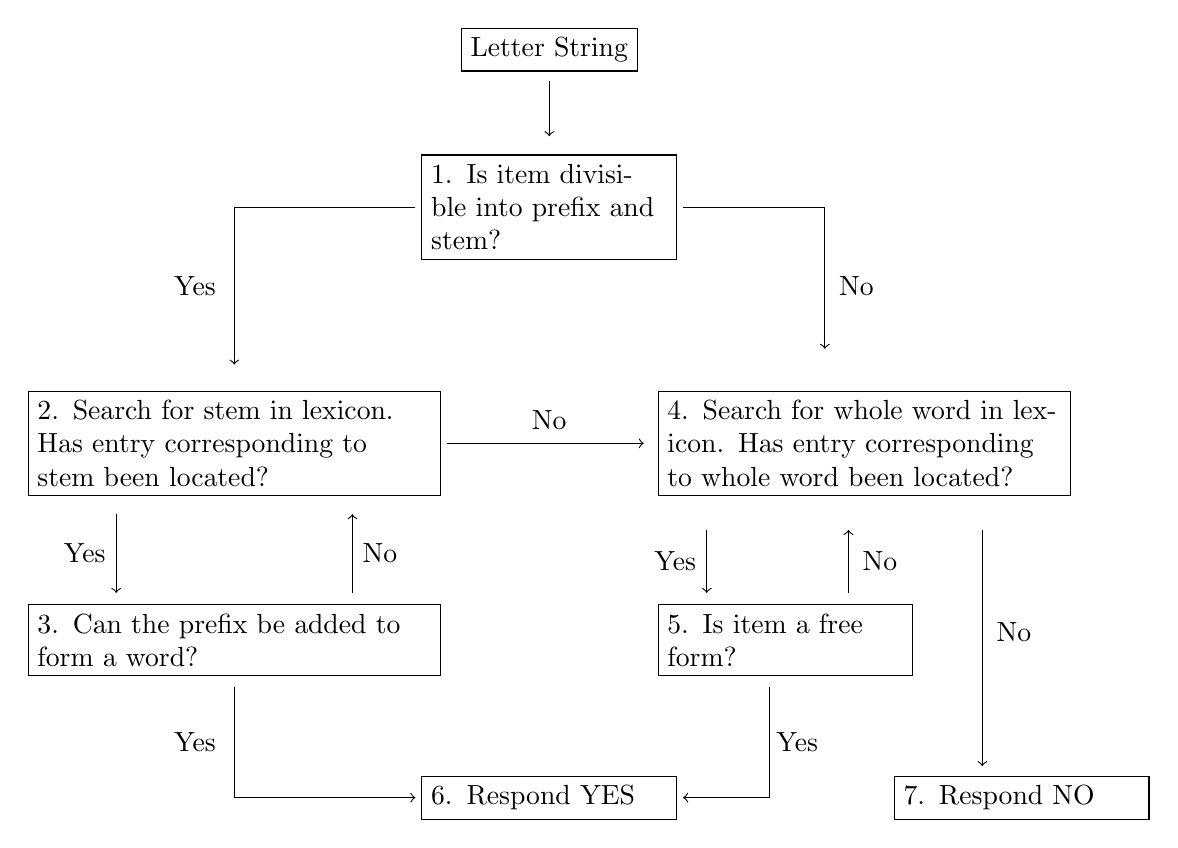
\begin{tikzpicture}%[scale=0.80]
\draw (5,8) node [shape= rectangle, draw] (signal) {Letter String};
\draw (5,6) node [text width=3cm, align=left, shape= rectangle,
draw] (first) {1. Is item divisible
  into prefix and stem?};
% \draw [->] (signal) -- (first);
\draw [->] (5,7.6) -- (5,6.9);
% Third row
\draw (1,3) node [text width=5cm, align=left, shape= rectangle,
draw] (second) {2. Search for stem in lexicon. Has entry corresponding
  to stem been located?};
\draw (9,3) node [text width=5cm, align=left, shape= rectangle,
draw] (fourth) {4. Search for whole word in lexicon. Has entry
  corresponding to whole word been located?};
\draw [-] (1,6) -- (3.3,6);
\draw [->] (1,6) -- (1,4);
% \draw [->] (first) -- (second);
% \draw [->] (first) -- (fourth);
\draw [-] (6.7,6) -- (8.5,6);
\draw [->] (8.5,6) -- (8.5,4.2);
\draw (8.9,5) node {No};
\draw (.5,5) node {Yes};
% \draw [->] (second) -- (fourth);
\draw [->] (3.7,3) -- (6.2,3);
\draw (5,3.3) node {No};

% Fourth row
\draw (1,.5) node [text width=5cm, align=left, shape= rectangle,
draw] (third) {3. Can the prefix be added to form a word?};
\draw (8,.5) node [text width=3cm, align=left, shape= rectangle,
draw] (fifth) {5. Is item a free form?};
% \draw [->] (second) -- (third);
\draw [->] (7,1.9) -- (7,1.1);
\draw [<-] (8.8,1.9) -- (8.8,1.1);
\draw [->] (-.5,2.1) -- (-.5,1.1);
\draw [<-] (2.5,2.1) -- (2.5,1.1);

\draw [->] (10.5,1.9) -- (10.5,-1.1);

\draw (-.9,1.6) node {Yes};
\draw (2.85,1.6) node {No};
% Fifth row
\draw (5,-1.5) node [text width=3cm, align=left, shape= rectangle,
draw] (first) {6. Respond YES};
\draw (11,-1.5) node [text width=3cm, align=left, shape= rectangle,
draw] (first) {7. Respond NO};
\draw [-] (1,-0.1) -- (1,-1.5);
\draw [->] (1,-1.5) -- (3.3,-1.5);
\draw [<-] (6.7,-1.5) -- (7.8,-1.5);
\draw [-] (7.8,-1.5) -- (7.8,-0.1);
\draw (.5,-.8) node {Yes};
\draw (8.15,-.8) node {Yes};
\draw (10.9,.6) node {No};
\draw (9.2,1.5) node {No};
\draw (6.6,1.5) node {Yes};
% % \node (context) {};
% \node [shape= rectangle, draw] (intermediate) [below=of signal]  {intermediate access representation};

% \node [shape= rectangle, draw] (access-rep) [below=of intermediate]  {access representation};
% \node [shape= rectangle, draw] (concept-nodes) [below=of access-rep]  {concept nodes};
% % \node (placeholder) [below=of concept-nodes]  {};
% \node [shape= rectangle, draw] (synsem-rep) [below=of concept-nodes]  {syntactic
%   representations \hspace*{2cm}semantic representations};
% % \node (syn-rep) [left=of placeholder]  {syntactic representations};
% % \node (sem-rep) [right=of placeholder]  {semantic representations};
% \node [shape= circle, draw] (output) [below=of synsem-rep]  {output};

% \draw [->] (signal) -- (intermediate);
% \draw [->] (intermediate) -- (access-rep);
% \draw [<->] (access-rep) -- (concept-nodes);
% \draw [<->] (concept-nodes) -- (synsem-rep);
% \draw [->] (synsem-rep) -- (output);

% \draw (-6.0,-4.9) rectangle (6,-1.6);
% \draw (-6.0,-8.7) rectangle (6,-5.4);

% \draw (-4.5,-2.15) node [text width=3cm, align=center] {segmentation and phonology}; 
% \draw (-4.5,-6.2) node [text width=3cm, align=center] {licensing and computation}; 

\end{tikzpicture}  
}

  \caption{Model for word recognition \citep{TaftandForster:1975}}
  \label{fig:taft_forster_word-recognition-model}
\end{center}
\end{figure}
\noindent
This model comes with 2 important features. First, it assumes that
morphological decomposition takes place in word recognition, the
relevant unit for the decomposition being the morpheme-level. Second,
it assumes that, for a specific string, only one specific
route is taken. That is, if a word is morphologically complex, it takes
the decompositional route, but if it is a simplex word, it takes the
whole-word route. 
While there have been many different responses to
their model, including e.g. \citet{ManelisandTharp:1977}, who rejected the very idea of
morphological decomposition in favor of whole-word look-up, the general
trend was soon towards mixed
models, that is, models that allow morphological decomposition and
whole-word look-up for the same items. An early example is the mixed model proposed in
\citet{Stannersetal:1979}, where one and the
same form can not only be stored in memory as a whole but can also at
least partially be
activated via a decompositional pathway.
\is{morphological decomposition|)}

% \citet{Stannersetal:1979}
% Using repetition priming combined with a lexical
% decision task, they investigated the English inflectional affixes \emph{-s},
% \emph{-ed} and \emph{-ing}, irregular past tense forms, and adjectival and
% nominal derivatives of verbs (e.g. \emph{selective/select} or
% \emph{appearance/appear}). In the interpretation of their findings, they argue
% that one plausible explanation lies in assuming that for regular inflection,
% the base form is accessed in memory, and the inflected form itself is not
% listed in memory, while in the other cases, the irregular or derived forms are
% stored in the lexical memory, but the verbal base is nevertheless partially
% activated, due to the interconnectness of the entries in the lexicon. 

% These early models did not focus on the role of semantic
% transparency. 
% However, semantic transparency plays a very important role in

A hugely influential and widely-cited model is the meta model for
morphological processing introduced in \citet{SchreuderandBaayen:1995}. This model is of additional interest, as it explicitly addresses problems relating to semantic transparency.
A schematic outline of this model, their
Figure 1, is reproduced in \figref{fig:schreuder_baayen_meta-model}.

% \resizebox{12cm}{!}{%
% \scalebox{.75}{%
\begin{figure}[h]
\begin{center}
\begin{tikzpicture}[>=stealth]
\node [shape= circle, draw] (signal) {speech signal};
% \node (context) {};
\node [shape= rectangle, draw] (intermediate) [below=of signal]  {intermediate access representation};

\node [shape= rectangle, draw] (access-rep) [below=of intermediate]  {access representation};
\node [shape= rectangle, draw] (concept-nodes) [below=of access-rep]  {concept nodes};
% \node (placeholder) [below=of concept-nodes]  {};
\node [shape= rectangle, draw] (synsem-rep) [below=of concept-nodes]  {syntactic
  representations \hspace*{2cm}semantic representations};
% \node (syn-rep) [left=of placeholder]  {syntactic representations};
% \node (sem-rep) [right=of placeholder]  {semantic representations};
\node [shape= circle, draw] (output) [below=of synsem-rep]  {output};

\draw [->,thick] (signal) -- (intermediate);
\draw [->,thick] (intermediate) -- (access-rep);
\draw [<->,thick] (access-rep) -- (concept-nodes);
\draw [<->,thick] (concept-nodes) -- (synsem-rep);
\draw [->,thick] (synsem-rep) -- (output);

\draw (-6.0,-4.9) rectangle (6,-1.6);
\draw (-6.0,-8.2) rectangle (6,-5.1);

\draw (-4.5,-2.25) node [text width=3cm, align=center] {segmentation and phonology}; 
\draw (-4.5,-5.8) node [text width=3cm, align=center] {licensing and computation}; 

\end{tikzpicture}  

  \caption{Meta model for morphological processing \citep{SchreuderandBaayen:1995}}
  \label{fig:schreuder_baayen_meta-model}
\end{center}
\end{figure}

\noindent
\citet{SchreuderandBaayen:1995} distinguish 3 stages:
segmentation, licensing, and combination. At the segmentation stage,
the speech input is mapped to access representations which are form-based representations of the speech signal. This is a 2-step
process, involving an intermediate access representation and, after segmentation, an access
representation proper. An
intermediate access representation might still contain more than one word,
whereas the access representation proper can at most correspond to one
complex word: ``Such `lexical' access
representations may be present for full complex forms, for stems,
whether bound or free, for affixes, and for clitics. They contain
modality-specific form information that is normalized both with
respect to the inherent variability in the speech signal and with
respect to the variability caused by phonological processes such as
vowel harmony and various kinds of assimilation
processes" \citep[133--134]{SchreuderandBaayen:1995}. 
The next 2 stages, licensing and computation, both take
place at the level of lexical representations. Lexical representations constitute the final output of the
lexicon. A lexical representation consists of a concept node,
which in turn is connected with syntactic and semantic
representations. The interplay between the concept nodes and these
syntactic and semantic representations constitutes one of the most
interesting aspects of the model. The concept node itself can be
understood as a bundling of links to specific syntactic and semantic
representations; concept nodes exist only for those concepts that
``receive verbal expression in the language at the form level"
\citep[136]{SchreuderandBaayen:1995}. That is, in this account,
lexical gaps like the missing liquid related counterpart to German \emph{satt} `full with respect to
food' don't have a concept node, though expressing a concept. Syntactic representations contain information on, among others,
subcategorization, word class, and argument structure.
\citet[136]{SchreuderandBaayen:1995} remain vague with respect to the
semantic representation (``specify various meaning aspects"). However,
in their figures and discussion it becomes clear that these various meaning aspects
are essentially what is responsible for the meaning of and meaning
differentiations between concept nodes. Semantic information is only
stored once, ``the links with the concept nodes serving as the
means for distinguishing and addressing concepts" \citep[140]{SchreuderandBaayen:1995}. 
\il{Dutch!{illustrating the Schroeder/Baayen model}|(}
Thus, the difference between Dutch
\emph{ruim} `spacious' and \emph{ruim-te} `space' is a difference in
the corresponding links to the syntactic and semantic representations,
which for \emph{ruim-te} include links to the syntactic node
NOUN, and to the semantic nodes ABSTRACT PROPERTY and SPACIOUSNESS,
cf. \citet[138]{SchreuderandBaayen:1995}.
 The link structure in this
model can be used to represent different degrees of semantic
transparency. This will become clearer when looking at how a novel
complex form leads to the generation of new lexical representations.

% In the case of monomorphemic words, the lexical
% representation is simply the concept node connected with the
% corresponding access representation, along with the concept's node
% associated syntactic and semantic representations. No licencing and
% composition is required in this case. 

% However, for novel complex
% forms, this mechanism ensures the generation of new lexical
% representations. 

How does the model deal with new complex combinations? Initially, at least 2
different access representations are activated, in turn leading to the
activation of the corresponding concept nodes. At this point, a
licensing mechanism checks whether the associated syntactic
presentations allow the system to proceed with meaning computation. In
particular, \citet[137]{SchreuderandBaayen:1995} distinguish 3
scenarios:
\begin{enumerate}
\item No new concept node is added if the meaning of a complex word
  can be obtained by the union of the relevant sets of
  representations. They exemplify this via Dutch plural formation by
  the regular plural \emph{-en} (e.g. \emph{boek} `book' $\rightarrow$ \emph{boek-en} `books').
\item A new concept node is created in any other case that involves computation.
\item Not fully semantically transparent forms also receive their own
  concept node.
\end{enumerate}

\is{frequency!{effects in the Schroeder/Baayen model}|(}
Note that word forms such as Dutch \emph{boek-en} `books', being transparent and
computable via set union, might nevertheless develop their own access
representations. \linebreak[3]Whether or not this happens is solely
frequency driven. However, even with their own access representation,
they will not develop a  concept node as long as their semantics
remains unchanged, that is, transparent.
\il{Dutch!{illustrating the Schroeder/Baayen model}|)}

The Schreuder/Baayen model uses spreading activation; as indicated in \figref{fig:schreuder_baayen_meta-model} by the double-headed
arrows, all levels except the intermediate access representations can
receive activation feedback from higher levels.  As \citeauthor{SchreuderandBaayen:1995} point out, this architecture
can account for a number of well-known frequency effects.
Word-frequency effects, for example, lead to higher activation levels of the
access representations, while the cumulative stem frequency effect is
best viewed as being due to heightened activation levels of the concept
node corresponding to the stem \citep[147]{SchreuderandBaayen:1995}. % cf. p. 147
\is{frequency!{effects in the Schroeder/Baayen model}|)}

\is{semantic transparency!{in the Schroeder/Baayen model}|(}
With regard to semantic transparency, \citet[140]{SchreuderandBaayen:1995} assume that ``a
semantically transparent relation between a complex word and its
constituents can be modeled as a substantial overlap between the set
of (semantic) representations of the complex word and the sets of
representations of its constituents".  In particular, empirical
effects of semantic transparency can be modeled via the flow of
activation (1)  between the concept nodes and the syntactic and
semantic nodes and (2) from the concept nodes to the access representations.

\il{Dutch!{illustrating the Schroeder/Baayen model}|(}
\citeauthor{SchreuderandBaayen:1995} illustrate the feedback to the concept
nodes with the help of the semi-transparent derivation \emph{groen-te} 
`vegetable' from \emph{groen} `green' and the abstract-noun forming
suffix \emph{te} and the fully transparent derivation \emph{trots-heid}
`pride', from \emph{trots} `proud/pride' and \emph{-heid}. For the
former, \citet[142]{SchreuderandBaayen:1995} assume that there is
hardly any activation from the semantic node of \emph{groente} to that
of \emph{groen}, since there are hardly any links between the concept
node of \emph{groente} and the semantic and syntactic nodes linked to
\emph{groen}. In contrast, for the latter, \emph{trotsheid}, both the concept node for
\emph{trots} as well as the one for \emph{-heid} will receive
activation feedback via the semantic representations shared with the
concept node of \emph{trotsheid}.  
\il{Dutch!{illustrating the Schroeder/Baayen model}|)}

The activation feedback from concept nodes to access representations is
proportional to the activation level of the concept nodes involved
\citep[142]{SchreuderandBaayen:1995}. That is, while for a
semantically transparent formation the highest extent of activation
feedback will flow from the concept node of the complex form itself to
its access representation, there will also be feedback from the
co-activated concept nodes to their respective access
representations. In contrast, for semantically opaque formations,
there will be little if any feedback to the individual constituents'
access representations, as the corresponding concept nodes are not
highly activated.

In addition, semantic transparency 
is hypothesized by \citet[146]{SchreuderandBaayen:1995} to also play a
role in the development of concept nodes for derivational
affixes. They predict an
earlier acquisition of transparent affixes, and they predict
the development of representations for bound stems only if these
participate in word formations that are compositional. % p. 147
% lexical representations 
\is{semantic transparency!{in the Schroeder/Baayen model}|)}

While \citet{SchreuderandBaayen:1995} are mainly concerned with
inflection and derivation, we can easily apply the model's general logic to
compounds. Thus, using \emph{bank barn} as an example of a novel
compound, the intermediate access representation % \emph{bank barn}, 
\textipa{[""b\ae NkbA:n]}
leads to the activation of the access representations for \emph{bank} and
\emph{barn}. These, in turn, lead to the activation of at least the
concepts BANK1 `institution that lends money etc.' and BANK2 `raised mass of earth', and BARN `farm outbuilding'. 
Based on the syntactic representations associated with the concept
nodes, meaning computation is licensed, since noun noun compounding is a 
 valid morphological operation in English. While it is partly the aim
of this work to find out how or to what extent one can compute a meaning
for these 2 items, it is clear that the computation involved will be
more than a simple set union. In fact, it seems a fair claim that all
compound formation surpasses a regular plural affix in complexity and
is typically more than just set union (recall that even the most
straightforward noun noun combination given in the introduction,
\emph{silk fabric}, already allows a construal with the \textsc{made of} relation). In consequence, this means that
after meaning computation, a new concept node BANK BARN will have come
into existence.

% The reasoning behind this model is best understood by first looking at a
% concrete example and then stepping through further features of the
% model. Thus, figure \ref{fig:cannibalizable} illustrates the processing of \emph{cannibalizable}.


    
  
% % \resizebox{12cm}{!}{%
% \scalebox{.80}{%
% \begin{figure}[h]
%   \begin{center}
% \begin{tikzpicture}
% \node [shape= circle, draw] (signal) {speech signal};
% % \node (context) {};
% \node [shape= rectangle, draw] (intermediate) [below=of signal]  {\textipa{""k\ae nIb@"laIz@bl}};
% \node (access-placeholder) [below=of intermediate]
% {};

% \node [shape= rectangle, draw] (access-rep-left) [left=of access-placeholder]
% {\textipa{"k\ae nIb@laIz}};
% \node [shape= rectangle, draw] (access-rep-right) [right=of access-placeholder]
% {\textipa{@bl}};


% \node [shape= rectangle, draw] (concept-node-left) [below=of access-rep-left]  {CANNIBALIZE};
% \node [shape= rectangle, draw] (concept-node-right) [below=of access-rep-right]  {ABLE};

% \node (concept-nodes-place) [below=of access-placeholder]  {};

% \node (synsem-rep-place) [below=of concept-nodes-place]  {};
% \node [shape= rectangle, draw] (synsem-rep-left) [below=of concept-node-left]  {syn/sem};

% \node [shape= rectangle, draw] (synsem-rep-right) [below=of concept-node-right]  {syn/sem};


% % \node (syn-rep) [left=of placeholder]  {syntactic representations};
% % \node (sem-rep) [right=of placeholder]  {semantic representations};
% \node [shape= circle, draw] (output) [below=2cm of synsem-rep-place]  {output};
% % \draw (0,-9) \node [shape= circle, draw] {output};

% \draw [->] (signal) -- (intermediate);
% % \draw [->] (intermediate) -- (access-rep);
% \draw [->] (intermediate) -- (access-rep-left);
% \draw [->] (intermediate) -- (access-rep-right);
% \draw [<->] (access-rep-left) -- (concept-node-left);
% \draw [<->] (access-rep-right) -- (concept-node-right);
% \draw [<->] (concept-node-left) -- (synsem-rep-left);
% \draw [<->] (concept-node-right) -- (synsem-rep-right);
% \draw [->] (synsem-rep-left) -- (output);
% \draw [->] (synsem-rep-right) -- (output);

% \draw (-6.0,-4.7) rectangle (6,-1.6);
% \draw (-6.0,-8.5) rectangle (6,-5.1);

% \draw (-4.5,-2.15) node [text width=3cm, align=center] {segmentation and phonology}; 
% \draw (-4.5,-7.7) node [text width=3cm, align=center] {licensing and computation}; 

% \end{tikzpicture}  
% \end{center}
% \label{fig:cannibalizable}
% \end{figure}
% In a first step, the speech signal is represented as an intermediate access
% represenation. Assuming for \emph{cannalizable} that it is a string
% encountered for the first time, but prosodically clearly recognizable as one
% rather low-level unit, the whole word constitutes the intermediate access
% representation. This representation, in turn, can be mapped onto two different
% access representation, standing for the base and the suffix,
% respectively. Both access representations are connected to their corresponding
% lexical representations, consisting of a concept node linked to its semantic
% and syntactic representation. It is now the work of the licensing and
% composition component to combine these two lexical representations and output
% a new lexical representation for the complex formation \emph{cannalizable}.


% I will come back to their model after discussing the psycholinguistic studies
% on the role of semantic transparency in compound processing.

% \fbox{
% \begin{minipage}{1.0\linewidth}
% \textbf{WOHIN DAMIT?}
%  As can be seen from the examples discussed above, complex nominals or, as the
% research was focussed on words, compounds, played no role in
% the development of these early models. However, compounds as a class seem to lend
% themselves further for investigation, especially when it comes to mixed
% models. Indeed, the high productivity of compound formation on the one hand
% and the high degree of opaqueness seen in compounds like \emph{buttercup}
% already make either of the first to models implausible. Manupilating a
% string's semantic transparency can then be used to get to a better
% understanding of the architecture of mixed models. 
 
% \end{minipage}
% }

% The role of compounds in model building


\citet{Libben:1998} introduces a model explicitly designed for
compounds, which in many aspects can be seen as building on the Schreuder/Baayen model. 
% \citet[33]{Libben:1998} argues that the Schreuder/Baayen model cannot easily handle
% assymmetries in the overlap of compounds and their constituents at the semantic level. We will come back to this point after presenting his model.  \textbf{WHY? COME BACK TO THIS POINT LATER}. 
\citet{Libben:1998}
distinguishes 3 levels: the stimulus level, the lexical
level, and the conceptual level.

The stimulus level is the level where morphological parsing takes
place. A left to right recursive parsing
  procedure checks both constituents for lexical status and thus
  avoids wrongly identifying a simplex word as a
  compound, e.g. dividing \emph{boycott} into \emph{boy} + \emph{cott}, while correctly identifying novel compounds, e.g. Libben's example
  \emph{redberry} (cf. \citealt{Libben:1994}, where he discusses a parser with these properties in detail).


Word forms, that is, stored representations of actual words, are represented at the lexical level. Libben illustrates
this level with the help of the existing
compounds \emph{strawberry} and \emph{blueberry}, the novel compound
\emph{redberry}, and the surname \emph{Thornberry}. \emph{Strawberry},
\emph{blueberry} and \emph{Thornberry} have representations at the
lexical level. In addition, the representations of
\emph{strawberry} and \emph{blueberry} have a structured
representation indicating their constituent
structure. In both cases, their 2 constituents are linked to
their respective lexical representations. In contrast, \emph{Thornberry} does
not have a structured representation and, consequentially, does not
contain links from \emph{thorn} and \emph{berry} to the respective
lexical entries. \emph{Redberry} does not have a representation at this level, as it is a new compound. 

\is{semantic transparency!{of constituents in Libben's model}|(}
The meanings are represented at the conceptual level. The links
between the lexical level and the conceptual level are used to model
constituent transparency. These links allow one to differentiate between
the \emph{straw} in \emph{strawberry} and the \emph{blue} in
\emph{blueberry}, both of which are linked to the respective
constituents at the lexical level, while only \emph{blue} is linked to
the corresponding entry at the conceptual level, too. Libben
distinguishes 8 different possible
configurations, with the first major distinction between componential
and noncomponential compounds. Componential compounds are endocentric
compounds. They can be paraphrased with the help of the pattern
`compound (noun 1 and noun 2/N1N2) is noun 2/N2', e.g. `a blueberry is a berry'. 
Noncomponential compounds do not allow this paraphrase (capturing
 the exocentric/bahuvrihi types in other classifications,
 cf. \citealt[Footnote 1]{Libben:1998}). Within both classes, Libben assumes a
 fourfold differentiation driven by constituent transparency: In the
 first configuration, transparent-transparent (TT), 
 both constituents are transparently related to the compound
 meaning. In the second configuration, transparent-opaque (TO), only the first constituent is
 transparent, whereas the second constituent is opaque. The third configuration, opaque-transparent (OT), shows the exact opposite arrangement: the first constituent is opaque and the second constituent is transparent. Finally, in the fourth configuration, both constituents are
 opaque, yielding opaque-opaque (OO) combinations. Libben's example for a
 componential TT compound is \emph{blueberry}. The componential TO and OT types are exemplified by \emph{shoehorn}
 and \emph{strawberry} respectively: The
 meaning of \emph{shoehorn}, `implement to be inserted at the heel of
 the shoe to ease the foot in', is not related to the meaning of
 \emph{horn}. Likewise, the meaning of \emph{strawberry} is not related to the meaning of
 \emph{straw}. Libben exemplifies the
 same 3 types for the noncomponential class, i.e., the
 non-endocentric compounds, with
 \emph{bighorn}, \emph{jailbird}, and \emph{yellow belly},
 respectively. A \emph{bighorn} is not a kind of horn, but a species
 of sheep with big horns. It is therefore noncomponential, but it is
 TT as the horns that are metonymically used to refer to the whole
 species are horns and are big. A \emph{jailbird} is no bird, but a
 person who is often or has been often in jail, therefore the first
 element is transparent. And a \emph{yellowbelly} is a coward, if,
 as Libben assumes, it is a noncomponential type OT, then he must have
 a paraphrase along the lines of `somebody with a bad or unsecure feeling in her
 belly' in his mind. 
% might be many
%  things, but what Libben must have had in mind for the TO
%  classification is probably one of its uses as an animal name, e.g.,
%  as the name for the yellow-bellied slider, a type of turtle, which
%  has yellow stripes, but not a yellow belly. 
% is a coward\texttt{[informal: a coward]}    

\citet{Libben:1998} does not give any examples for OO types in this
article. \citet{Libbenetal:2003} uses \emph{hogwash} `nonsense' to
exemplify the OO category. Conceptually, it is hard to see how one would
distinguish between componential and noncomponential types of OO
compounds from a
synchronic vantage point: if semantically neither constituent is
related to the compound meaning, the differentiation between
componential and noncomponential compounds becomes useless, even
though historically one could perhaps argue for componential vs.
noncomponential pathways of meaning development.

\enlargethispage{3\baselineskip}
Figures \ref{fig:libben-1998-TT-comp}--\ref{fig:libben-1998-OT-non}
reproduce his representation for the 3 non-OO types in the
noncomponential and componential versions, containing the links between and
within levels, cf. Figure 3, \citet[38]{Libben:1998}.
\pagebreak
% \vspace*{1cm}

% The following figures are set side by side using minipages inside a tabularx environment
% Every 2 figures are set in their own tabularx. The captions lead to overfull hboxes, probably due to scaling issues.
%
% \hspace*{-1.5cm}
% \begin{tabular}[!htb]{p{7cm}@{\hspace{.3cm}}p{7cm}}
% \noindent
% \begin{tabularx}{1\textwidth}{|X|X|}
% what&what\\
% \end{tabularx}
\noindent
\begin{tabularx}{1\textwidth}{XX}
%\fbox{
\begin{minipage}[t]{5.4cm}
% \begin{center}
% \hspace*{-1cm}
\resizebox{5.4cm}{!}{%
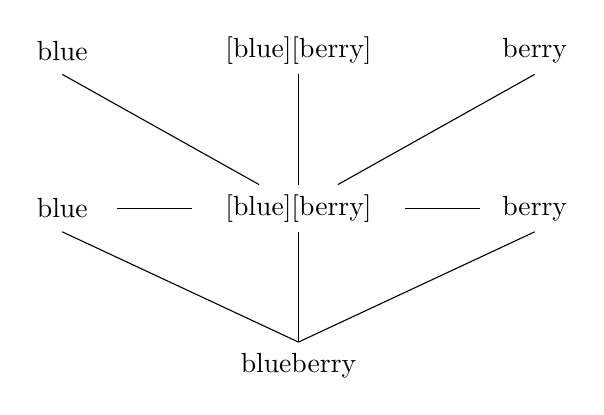
\begin{tikzpicture}
\draw (0,4) node [align=center] {[blue][berry]}; 
\draw (-3,4) node [align=center] {blue}; 
\draw (3,4) node [align=center] {berry}; 

\draw (0,2) node [align=center] {[blue][berry]}; 
\draw (-3,2) node [align=center] {blue}; 
\draw (3,2) node [align=center] {berry}; 

\draw (0,0) node [align=center] {blueberry}; 

\draw [-] (0,0.3) to  (0,1.7);
\draw [-] (0,0.3) to  (3,1.7);
\draw [-] (0,0.3) to  (-3,1.7);

\draw [-] (1.35,2) to  (2.3,2);
\draw [-] (-1.35,2) to  (-2.3,2);

\draw [-] (0,2.3) to  (0,3.7);
\draw [-] (0.5,2.3) to  (3,3.7);
\draw [-] (-0.5,2.3) to  (-3,3.7);
\end{tikzpicture}  
}
\captionsetup{font=small,justification=raggedright,singlelinecheck=on}
\captionof{figure}{TT componential}
%  \caption{Libben (1998): Constituency and componentiality at the lexical and conceptual levels}
  \label{fig:libben-1998-TT-comp}
% \end{center}
% \end{figure}
  
\end{minipage}%}
&
%\fbox{
\begin{minipage}[t]{5.4cm}
% \begin{figure}[h]
% \begin{figure}
% \begin{center}
% \hspace*{-1cm}
\resizebox{5.4cm}{!}{%
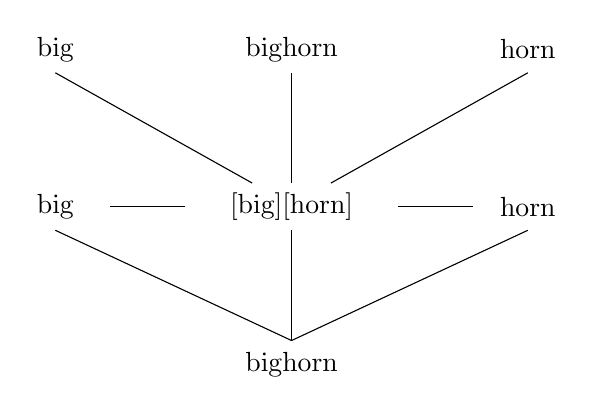
\begin{tikzpicture}
\draw (0,4) node [align=center] {bighorn}; 
\draw (-3,4) node [align=center] {big}; 
\draw (3,4) node [align=center] {horn}; 

\draw (0,2) node [align=center] {[big][horn]}; 
\draw (-3,2) node [align=center] {big}; 
\draw (3,2) node [align=center] {horn}; 

\draw (0,0) node [align=center] {bighorn}; 

\draw [-] (0,0.3) to  (0,1.7);
\draw [-] (0,0.3) to  (3,1.7);
\draw [-] (0,0.3) to  (-3,1.7);

\draw [-] (1.35,2) to  (2.3,2);
\draw [-] (-1.35,2) to  (-2.3,2);

\draw [-] (0,2.3) to  (0,3.7);
\draw [-] (0.5,2.3) to  (3,3.7);
\draw [-] (-0.5,2.3) to  (-3,3.7);


\end{tikzpicture}  
}
\captionsetup{font=small,justification=raggedright,singlelinecheck=on}
\captionof{figure}{TT noncomponential}
%  \caption{Libben (1998): Constituency and componentiality at the lexical and conceptual levels}
  \label{fig:libben-1998}
% \end{center}
% \end{figure}
  
\end{minipage}
%}
% \end{tabular}
\end{tabularx}
\vspace*{1cm}

\noindent
\begin{tabularx}{1\textwidth}{XX}
%\fbox{
\begin{minipage}[t]{5.4cm}
\resizebox{5.4cm}{!}{%
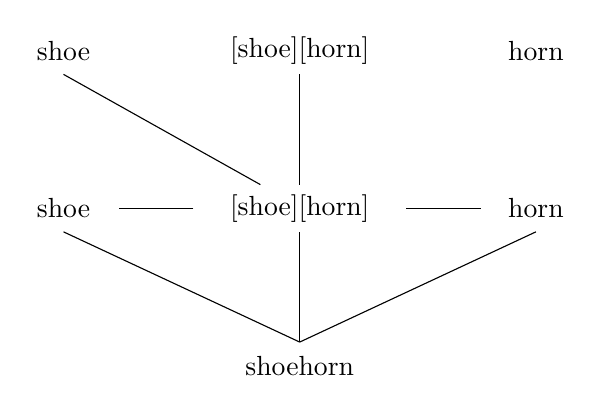
\begin{tikzpicture}
\draw (0,4) node [align=center] {[shoe][horn]}; 
\draw (-3,4) node [align=center] {shoe}; 
\draw (3,4) node [align=center] {horn}; 

\draw (0,2) node [align=center] {[shoe][horn]}; 
\draw (-3,2) node [align=center] {shoe}; 
\draw (3,2) node [align=center] {horn}; 

\draw (0,0) node [align=center] {shoehorn}; 

\draw [-] (0,0.3) to  (0,1.7);
\draw [-] (0,0.3) to  (3,1.7);
\draw [-] (0,0.3) to  (-3,1.7);

\draw [-] (1.35,2) to  (2.3,2);
\draw [-] (-1.35,2) to  (-2.3,2);

\draw [-] (0,2.3) to  (0,3.7);
% \draw [-] (0,2.3) to  (3,3.7);
\draw [-] (-0.5,2.3) to  (-3,3.7);


\end{tikzpicture}  
}
\captionsetup{font=small,justification=raggedright,singlelinecheck=on}
\captionof{figure}{TO componential}
%  \caption{Libben (1998): Constituency and componentiality at the lexical and conceptual levels}
  \label{fig:libben-1998}
\end{minipage}
% }
&
\begin{minipage}[t]{5.4cm}
\resizebox{5.4cm}{!}{%
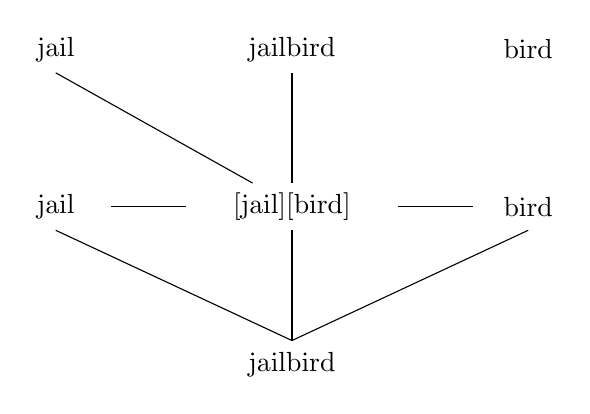
\begin{tikzpicture}
\draw (0,4) node [align=center] {jailbird}; 
\draw (-3,4) node [align=center] {jail}; 
\draw (3,4) node [align=center] {bird}; 

\draw (0,2) node [align=center] {[jail][bird]}; 
\draw (-3,2) node [align=center] {jail}; 
\draw (3,2) node [align=center] {bird}; 

\draw (0,0) node [align=center] {jailbird}; 

\draw [-] (0,0.3) to  (0,1.7);
\draw [-] (0,0.3) to  (3,1.7);
\draw [-] (0,0.3) to  (-3,1.7);

\draw [-] (1.35,2) to  (2.3,2);
\draw [-] (-1.35,2) to  (-2.3,2);

\draw [-] (0,2.3) to  (0,3.7);
% \draw [-] (0,2.3) to  (3,3.7);
\draw [-] (-0.5,2.3) to  (-3,3.7);


\end{tikzpicture}  
}
\captionsetup{font=small,justification=raggedright,singlelinecheck=on}
\captionof{figure}{TO noncomponential}
%  \caption{Libben (1998): Constituency and componentiality at the lexical and conceptual levels}
  \label{fig:libben-1998_TOnoncomponential}
\end{minipage}
\end{tabularx}
\vspace*{1cm}

% \hspace*{-1.5cm}
\noindent
\begin{tabularx}{1\textwidth}{XX}
\begin{minipage}[t]{5.4cm}
\resizebox{5.4cm}{!}{%
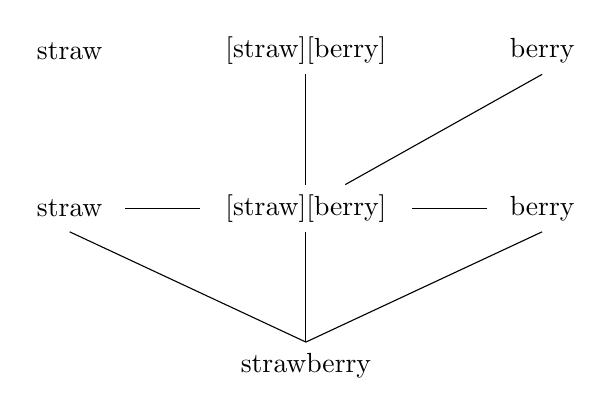
\begin{tikzpicture}
\draw (0,4) node [align=center] {[straw][berry]}; 
\draw (-3,4) node [align=center] {straw}; 
\draw (3,4) node [align=center] {berry}; 

\draw (0,2) node [align=center] {[straw][berry]}; 
\draw (-3,2) node [align=center] {straw}; 
\draw (3,2) node [align=center] {berry}; 

\draw (0,0) node [align=center] {strawberry}; 

\draw [-] (0,0.3) to  (0,1.7);
\draw [-] (0,0.3) to  (3,1.7);
\draw [-] (0,0.3) to  (-3,1.7);

\draw [-] (1.35,2) to  (2.3,2);
\draw [-] (-1.35,2) to  (-2.3,2);

\draw [-] (0,2.3) to  (0,3.7);
\draw [-] (0.5,2.3) to  (3,3.7);
% \draw [-] (0,2.3) to  (-3,3.7);


\end{tikzpicture}  
}
\captionsetup{font=small,justification=raggedright,singlelinecheck=on}
\captionof{figure}{OT componential}
%  \caption{Libben (1998): Constituency and componentiality at the lexical and conceptual levels}
  \label{fig:libben-1998}
\end{minipage}
&
\begin{minipage}[t]{5.4cm}
\resizebox{5.4cm}{!}{%
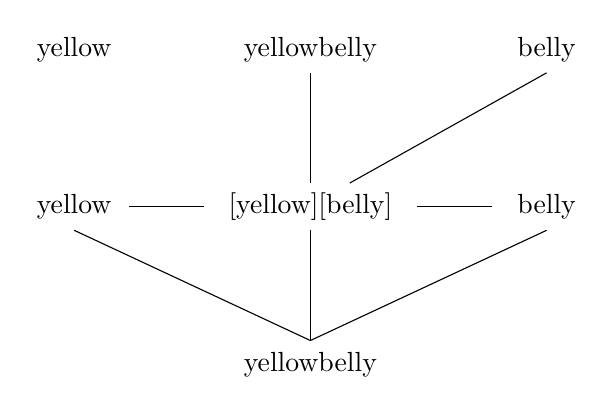
\begin{tikzpicture}
\draw (0,4) node [align=center] {yellowbelly}; 
\draw (-3,4) node [align=center] {yellow}; 
\draw (3,4) node [align=center] {belly}; 

\draw (0,2) node [align=center] {[yellow][belly]}; 
\draw (-3,2) node [align=center] {yellow}; 
\draw (3,2) node [align=center] {belly}; 

\draw (0,0) node [align=center] {yellowbelly}; 

\draw [-] (0,0.3) to  (0,1.7);
\draw [-] (0,0.3) to  (3,1.7);
\draw [-] (0,0.3) to  (-3,1.7);

\draw [-] (1.35,2) to  (2.3,2);
\draw [-] (-1.35,2) to  (-2.3,2);

\draw [-] (0,2.3) to  (0,3.7);
\draw [-] (0.5,2.3) to  (3,3.7);
% \draw [-] (0,2.3) to  (-3,3.7);


\end{tikzpicture}  
}
\captionsetup{font=small,justification=raggedright,singlelinecheck=on}
\captionof{figure}{OT noncomponential}
%  \caption{Libben (1998): Constituency and componentiality at the lexical and conceptual levels}
  \label{fig:libben-1998-OT-non}
\end{minipage}
\end{tabularx}
\vspace*{.5cm}


\noindent
The links within a level and between levels are always facillatory. The absence of links creates competition, leading to the eventual inhibition of non-targets.

% Comparison to the Schreuder-Baayen model
\citet[33]{Libben:1998} appears to endorse the operationalization of
semantic transparency proposed in
\citet[140]{SchreuderandBaayen:1995} (see above), that is, that
semantic transparency can be modeled as overlap between the semantic
representations of a complex word and the semantic representations of its
constituents. Furthermore, his stimulus level
corresponds to the level of access representations in the
Schreuder/Baayen model. It is in the higher levels that the 2 models
diverge, with Libben contending that the Schreuder/Baayen model does not ``easily
handle asymmetries in this overlap" \citep[33]{Libben:1998}.  He does
not clarify which asymmetries exactly he views as problematic. If one
considers his 3 examples for the componential types,
\emph{blueberry}, \emph{shoehorn}, and \emph{strawberry}, the core
difference between the 3 types of compounds lies in  the links
between lexical and conceptual level, with \emph{blueberry} linking to
both constituents' conceptual representation, whereas the other 2 compounds only
link to the respective transparent constituent's representation. On
the lexical level, they are alike insofar as their structured
representation is linked to the representations of the corresponding
constituents, in contrast to Libben's assumption for
\emph{Thornberry}. In the Schreuder/Baayen model, the 3 types
can be distinguished via their different connection strength to
semantic representations shared with the concept nodes of the
constituents, while their constituent structure is discernable
due to the interplay between access representations and concept
nodes. It is not clear to me how to best represent \emph{Thornberry}
in the Schreuder/Baayen model. However, as far as I can see, there is
also no empirical evidence to show that it behaves differently from,
e.g., OO compounds. All in all, while Libben's discussion is a helpful
clarification of the different types of compounds one can find, it
seems that his remark with regard to the observed asymmetry is of
greater relevance in distinguishing compound semantics from the
patterns found in derivation and inflection, but does not pose any
specific problem for the general structure of the Schreuder/Baayen model.
\is{models of morphological processing!{morpheme-based}|)}
\is{semantic transparency!{of constituents in Libben's model}|)}


% : ``An assumption crucial to the
% theory developed here is that a semantically transparent relation
% between complex word and its constituents can be modeled as a
% substantial overlap between the set of (semantic) representations of
% the complex word and the sets of representations of its
% constituents". However, he does This
% point will be discussed in detail in section \textbf{BLABLA}.



\subsection{Models without morphemes}
\label{sec:non-classical}
\is{models of morphological processing!{without morphemes}|(}
From the 1980s onward, alternative models of morphological
processing have been developed that differ radically from the
models discussed so far. Technically, the most important difference is
that morphemes are not represented as distinct
representational entities anywhere in these models. As far as their
empirical coverage is concerned, many
models, especially if they are actually implemented, model only very
specific aspects of morphological processing.  Most of the models
do  not target compounds in particular. Here, I present the main ideas
behind the very
influential models of \citet{RumelhartandMcClelland:1986} and
\citet{Bybee:1995} and then discuss in detail the amorphous model
proposed in \citet{Baayenetal:2011}, which addresses compound
processing as well as the issue of semantic transparency.

% Most of the discussion with regard to these models, however,
% has taken place against the background of inflection and derivational
% morphology, with one very prominent line of discussion being concerned
% mainly with the treatment of regular vs. irregular morphology. Here,
% non-classical models have been mainly argued against views from Pinker
% and colleagues, who, for the English regular and irregular past tense,
% argued for a symbolic rule for the regular cases and lexical
% representations for the irregular cases. These models are referred to
% in \citet[427]{Bybee:1995} as dual-processing models. \textbf{ADD Sources!}

%%%%%%%%%%%%%%%%%%%%%%%%%%%%%%%%%%%%%%%%%%%%%%%%%%%%%%%%%%%%%%%%%%%%%%%%
%%
%%            Rumelhart and McClelland
%%
%%%%%%%%%%%%%%%%%%%%%%%%%%%%%%%%%%%%%%%%%%%%%%%%%%%%%%%%%%%%%%%%%%%%%%%%

% \subsubsection{Rumelhart and McClelland 1986}
\subsubsection{Rumelhart and McClelland}
\label{sec:rumel}


\citet{RumelhartandMcClelland:1986} proposed a connectionist model in order to model the time course
of learning the past tense forms of English irregular and regular
verbs.
% \citet{RumelhartandMcClelland:1986} 
Their model is a response to views on
inflection in English that assume that part of acquiring morphology is
acquiring, or inducing, rules (they point to \citealt{Pinker:1984} as
an example of a model based on this view). English past tense formation is of
particular interest in this respect, because the regular
past tense formation via the addition of \emph{-ed} to the end of a
verb can be seen as a typical example of word form formation by rule. In consequence, the language learner will at one point have
learned this specific rule. In contrast, in their model, such a rule
is never explicitly stated anywhere, but the same behavior falls out
from properties of the model. % Note that in contrast to the models discussed before, this 
The model is
very restricted in its domain, since its goal is only to produce the
phonological representation of the past tense from the phonological
representations of the root form. However, this allows one to clearly
see which core aspects are important for this and similar
models. 
\figref{fig:RumelhartMcClelland}, their Figure 1, shows the basic structure of their model.
\begin{figure}[h]
  \centering
% Declare layers
\pgfdeclarelayer{background}
\pgfsetlayers{background,main}

\resizebox{\textwidth}{!}{%
% Styles
\tikzstyle{information text}=[text badly centered,font=\small,text width=3cm]
\begin{tikzpicture}[scale=.8,cap=round]
    % The graphic
    \begin{scope}[>=stealth', line width=1pt]
        \draw[->] (1,.9) node[below, information text]
            {Phonological representation of root form } -- (1,1.8);
        \draw[->] (5,-.2) node[below,information text]
            {Wickelfeature representation of root form } -- (5,.8);
        \draw[->] (11,-.2) node[below,information text]
            {Wickelfeature representation of past tense } -- (11,.8);
        \draw[->] (16,0.9) node[below,information text]
            {Phonological representation of past tense } -- (16,1.8);
    \end{scope}
    \draw (3,6) node[information text] { Fixed Encoding Network };
    \draw (8,6) node[information text, text width=4cm, ]
        { Pattern Associator Modifiable Connections };
    \draw (13.5,6) node[information text] { Decoding/Binding Network };
    % draw the nodes
    \foreach \x in {1,16}
        \foreach \y in {2,3,4} {
        \filldraw[fill=white] (\x,\y) circle (0.1);
        }
    \foreach \x in {5,11}
        \foreach \y in {1,2,3,4,5} {
            \filldraw[fill=white] (\x,\y) circle (0.1);
        }
    % The lines connecting the nodes are drawn in the background layer.
    % This way we can hide the lines behind the nodes and don't worry
    % about the width of each node.    
    \begin{pgfonlayer}{background}
        % we add the lines for the nodes starting in y 2,3, and 4
        \foreach \xa / \xb in {1 / 5, 5 / 11 , 11 / 5 , 16 / 11}
            \foreach \ya / \yb / \yc / \yd / \ye in {2 / 3 / 4 / 5 / 1, 
            3 / 4 / 5 / 1 / 2, 4 / 5 / 1 / 2 / 3} {
                \draw (\xa,\ya) -- (\xb,\ya);
                \draw (\xa,\ya) -- (\xb,\yb);
                \draw (\xa,\ya) -- (\xb,\yc);
                \draw (\xa,\ya) -- (\xb,\yd);
                \draw (\xa,\ya) -- (\xb,\ye);
            }
        % add remaining lines from y1 to y5
        \foreach \xa / \xb in {5 / 11 , 11 / 5}
            \foreach \ya / \yb in {1 / 5, 5 / 1} {
            \draw (\xa,\ya) -- (\xb,\ya);
            \draw (\xa,\ya) -- (\xb,\yb);
        }
    \end{pgfonlayer}
\end{tikzpicture}
}
% Author: Robert Felty
% Source: http://blog.robfelty.com/2007/02/14/pgf-gallery
% Model structure from Rumelhart \& McClelland (1986, p .222)%
% \textbf{MENTION SOMEWHERE THE SOURCE FOR THE CODE! -> acknowledgements}
%  http://www.texample.net/tikz/examples/about/
  \caption{A connectionist model for the English past tense \citep[222]{RumelhartandMcClelland:1986}. The \LaTeX {} code for the reproduction of their figure was written by Robert Felty and is available at \url{http://www.texample.net}.}
\label{fig:RumelhartMcClelland}
\end{figure}

Of particular interest are the levels of representation they assume,
the mechanism that links the levels, and the way the model learns. 
% I will discuss both of them in turn.
%As can be seen in figure \ref{fig:RumelhartMcClelland},
\citet{RumelhartandMcClelland:1986} distinguish
 4 different levels, 2 for the
phonological representations and 2 for so-called Wickelfeature
representations. These representations are paired, that is, there is a
phonological representation and a Wickelfeature representation of the
root form of an English
verb, and a phonological representation and a Wickelfeature
representation of the past tense of an English verb.
The Wickelfeature representations are  feature-based
representations of 3-phone
sequences, the Wickelphones, named by \citet{RumelhartandMcClelland:1986} after the proposal in 
\citet{Wickelgren:1969}.
% http://www.columbia.edu/~nvg1/Wickelgren/
The decoding and encoding networks are fixed, that is, there is no
variation in how the input phonemic representations are translated
into Wickelfeatures, nor is there variation in how the output Wickelfeature representations
are mapped on the output phonemic representations.

The core
of this model is the pattern associator which contains modifiable
connections between the input units,
that is, the Wickelfeature representations of the root forms, and the
output units, the Wickelfeature representations of the output
forms. Whether a unit is turned on or not depends on a probability
function which in turn depends on threshold values of the units and
the input they receive. Importantly, the units on the same level have
no interconnections and there is also no feedback in this
model. With this rather simple model architecture, many core
characteristics of learning the English past tense could be correctly modeled.

%%%%%%%%%%%%%%%%%%%%%%%%%%%%%%%%%%%%%%%%%%%%%%%%%%%%%%%%%%%%%%%%%%%%%%
%%
%%  BYBEE 1995 regular morphology and the lexicon
%%
%%%%%%%%%%%%%%%%%%%%%%%%%%%%%%%%%%%%%%%%%%%%%%%%%%%%%%%%%%%%%%%%%%%%%%

\subsubsection{Bybee's network model}
\label{sec:bybee}

Bybee's network model was originally proposed in \citet{Bybee:1985}
and \citet{Bybee:1988} (as \citealt[428]{Bybee:1995} points out, a model
with the same properties was proposed in \citealt{Langacker:1987} and \citealt{Langacker:1988}). Here, I follow her overview in
\citet[428--431]{Bybee:1995}. 

% \citet[428-431]{Bybee:1995} gives a summary of the core properties of her network model.
The network model is word-based, it can thus be seen as a lexicon
organized as a network. In this lexicon, words  have varying degrees of
lexical strength. The prime factor determining lexical strength is a word's token frequency. 
Words are related to other words via sets of
lexical connections between identical and similar phonological and
semantic features. While the words are not broken up into their
constituent morphemes, a morphological structure emerges due to the
intra-lexical connections. The lexical connections vary in
strength. Factors that influence connection strength are the type and
the number of shared features, and the token frequency of a specific
word. \is{frequency!{in Bybee's network model}|(}
% High-frequency words are easy to access,  serve as bases of
% morphological relations, 
Bybee argues that high frequency words  have greater lexical autonomy,
which is reflected in weaker
connections to other words. This idea is ``based on the common-sense
observation that items that are of high frequency in the input can be
learned on their own terms, while lower-frequency items are better
learned in relation to existing items" \citep[429]{Bybee:1995}. She further argues that phenomena such as suppletion and the known
resistance of high frequency irregulars to change are both linked to
lexical autonomy.
\is{frequency!{in Bybee's network model}|)}

Sets of words with similar patterns of semantic and phonological
connections reinforce each other, leading to emergent generalizations,
which are also refered to as schemata. Whether or not a schema is extended to other words
depends on the defining properties of the schema, e.g. whether it is
very general or very specific, and the strength of the schema,
which is derivable from the number of items that reinforce the
schema. \citet{Bybee:1995} distinguishes 2 types of schemas.
Source-oriented schemas generalize over pairs of basic and derived
forms. ``These correspond roughly to generative rules, since they can be
thought of as instructions for how to modify one form in order to
derive another" \citep[430]{Bybee:1995}. The regular past
tense formation in English with the suffix \emph{-ed} is captured by such a schema.

Product-oriented schemas, in contrast, are
generalizations over sets of complex/derived forms. Bybee exemplifies
this type of schema with the help of sub-regularities in English past
tense irregulars, e.g. the subclass containing \emph{strung, stung, flung, hung} etc. 
% this is Bybees example!
Membership in
these schemas, so Bybee,
is based on \isi{family resemblance}.

Bybee herself has not implemented her model; however, she 
states: ``Connectionist simulations could be thought of as testing
some of the properties of the network model and Langacker's cognitive
grammar, but the model itself is more complex and accounts for more
phenomena than any existing connectionist model''
\citep[428]{Bybee:1995}. Besides connectionist models, analogical
models come to mind as candidates for the implementation of the
product oriented schemas. Analogical models have been successfully used for some morphological phenomena (e.g. \citealt{Arndt-Lappe:2011} for stress assignments in English noun noun compounds or \citealt{Arndt-Lappe:2014} for the affix rivalry between English \emph{-ity} and \emph{-ness}).
%  AM algorithm, Skousen \& 
% Stanford, 2007)

\subsubsection{\citet{Baayenetal:2011}}
\label{sec:baayen2011}

\citet{Baayenetal:2011} present a very ambitious implemented
morphological model, the naive discriminative reader. It is of particular interest for my work, because
in some of the simulations run with the model, the issue of semantic
transparency is explicitly addressed. In contrast, the triangle model of
\citet{HarmandSeidenberg:2004}, aspects of which the naive
discriminative reader follows (cf. \citealt[439--440]{Baayenetal:2011}), does not address this
issue. Here, I aim at explaining its general structure, while
focusing on the place of semantic transparency in this model. 

The modeling target of Baayen et al's (2011) model are morphological effects in
visual comprehension, which they assess by using \isi{lexical decision} data.
% that is, as far as experimental effects are
% concerned, its scope is restricted to lexical decision.
% structure
It is a 2-layered symbolic network model, with unigrams and bigrams
as cues, and meanings as outcomes. Key to the model is the learning algorithm of
\citet{WagnerandRescorla:1972}. 
In \citet{Baayenetal:2011}, the modeling focuses on the end stage of the
lexical 
learning process: the cues, unigrams and bigrams, are already
associated with the outcomes, the meanings. These meanings range from word meanings
to inflectional and affixal meanings, that is, nominative case as well
as whatever a suffix such as \emph{-ness} stands for are meanings. Since the model has been
trained, it 
is in a state of equilibrium. 

Following \citeauthor{Baayenetal:2011}'s (\citeyear[450]{Baayenetal:2011}) representation, 
the association strength $V_{i}^{t + 1}$ from a cue $C_{i}$ at time
$t + 1$ results from its previous association strength $V_{i}^{t}$ plus the change in
association strength $\Delta V_{i}^{t}$. The change in association
strength is calculated according to the equation in \Next,
cf. \citet[450]{Baayenetal:2011}.\footnote{Note that I adjusted the
  index in the first if-statement to the index of the cue under
  discussion, $C_{i}$. This seems to be a mistake in the equation in
  \citet[450]{Baayenetal:2011}, cf. also equation (2) in
  \citet[299]{Baayen:2011}, where the index is set to the cue under discussion.}


\ex.  
\resizebox{.9\textwidth}{!}{%
$\Delta V_{i}^{t} =
\begin{cases}
  0 &\mbox{if ABSENT}(C_i,t)\\ % corrected after the equation in corpus linguistics and naive discriminative learning \citet[299]{Baayen:2011}
% \\
\alpha_i  \beta_1(\lambda -\Sigma_{\text{PRESENT}(C_j,t)}V_j) &\text{if
  PRESENT}(C_j,t) \;\&\; \mbox{PRESENT}(O,t)\\
\alpha_i, \beta_2(0 -\Sigma_{\text{PRESENT}(C_j,t)}V_j) &\text{if PRESENT}(C_j,t)\; \& \;\mbox{ABSENT}(O,t)\\
\end{cases}
$}\\\vspace*{.5em}
{}\\
% Calculating the change in association strength with the help of the
% Rescorla-Wagner equations; 
ABSENT/PRESENT: cue/outcome is absent or present;\\ standard settings for the parameters:
$\lambda$ = 1, all $\alpha$'s equal, $\beta_1$ = $\beta_2$
% checked, this is how it is


The first condition states that there is no change in association
strength from a cue $C_{i}$ to an outcome if the cue is absent. The
second and third conditions handle the changes in association strength
from cue $C_{i}$ to an outcome when the cue is present. If the cue
co-occurs with the outcome, the change in association strength is
positive and the cue's activation strength increases. If the cue
occurs, but the outcome is absent, its association strength decreases.

Both changes in activation strength depend on the number and
activation strength of other cues that are present. In particular, the higher
the summed activation levels of other cues present, the lower
the change in activation strength for cue $C_{i}$ if the outcome is present; if
the outcome is absent, the higher
the summed activation levels of other cues present, the higher the
negative change in activation strength for cue $C_{i}$.

\citet[450]{Baayenetal:2011} point out that at the end of its
learning, ``[t]he Rescorla-Wagner algorithm provides the
maximum-likelihood estimates of the weights on the connections between
letter unigrams and bigrams and word meanings."
To derive the association weights in the system in a stable state,
reaching an equilibrium, \citet{Baayenetal:2011} use a method
developed in \citet{Danks:2003}, who showed that solving the equation
in \Next, reproducing (9) in \citet{Baayenetal:2011}, allows one to derive the association strengths of the individual
cues.

\ex.
% \begin{equation*}
\( \displaystyle Pr(O|C_j) - \sum_{j=0}^{n}{Pr(C_j|C_i)V_j} = 0 \)  
% \end{equation*}
\\ $Pr(O|C_j)$ represents the conditional probability of the outcome
given cue C$_i$, and $Pr(C_j|C_i)$ the conditional probability of
cue C$_j$ given cue C$_i$. 

In order to solve this equation, \citet{Baayenetal:2011} for
simplicity's sake assume that the association strengths from letter
uni- and bigrams to meanings are modeled independently from all other
outcomes. They therefore refer to their model as a naive model, in
reference to the similarly simplifying assumption of conditional
independence for naive Bayes classifiers.

% Equilibrium training
In order to create a model in equilibrium, the authors proceeded as
follows:
\begin{enumerate}
\item They created a lexicon of 24,710 word types by selecting lexical
  items from \isi{CELEX} (cf. \citealt{Baayenetal:1995}) and from a number of
  individual psycholinguistic studies. All inflectional forms were
  also included.
\item The selected words were inserted into 13 different contexts and
  the resulting search patterns were used to extract a phrasal lexicon
  from the \isi{BNC}, consisting of 11,172,554 phrase tokens.
\item The connection weights for the Rescorla-Wagner network were
  calculated on the basis of this lexicon and the equilibrium equations.
\end{enumerate}
%   \frametitle{Equilibrium training}
%   \begin{itemize}
%   \item CELEX:
%     \begin{enumerate}
%     \item All monomorphemic nouns, verbs, adjectives 
%     \item All compounds/derived forms with items in 1. as base
%     \item All of these word's inflectional forms

%     \end{enumerate}

%   \item word stimuli from a number of studies
%   \item[$\rightarrow$] lexicon of 24710 word types
%   \item BNC:
%     \begin{itemize}
%     \item lexicon plugged into context: retrieved occurences plus preceding
%    words from BNC 
%     \item Resulting phrasal lexicon corresponding to quarter of corpus in
%   token size
%     \item Equilibrium equations for Rescorla-Wagner network solved with this
%   phrasal lexicon $\rightarrow$ weights are set
%     \end{itemize}


%   \end{itemize}
% \end{frame}

% Simulations
\citet{Baayenetal:2011} used the trained network to run a number of
simulations investigating simple words, inflected words, derived words, pseudo-derived words, compounds, and some phrasal effects. The general procedure is always the same:
\begin{enumerate}
\item Selecting
the empirical target and modeling it with regression models. \\
They first select reaction times from published \isi{lexical decision} experiments and
from the English Lexicon Project (cf. \citealt{Balotaetal:2007}). This
empirical data is modeled using regression models, taking
established predictors from the literature.
\item Simulating the empirical target and modeling the simulated
  data.\\ They select a stand-in for the empirical reaction times
  (derived from the activation levels of the network output). Then,
  they use the same regressors in regression models for the simulated data and compare the
  resulting models with the models for the empirical data. 
\end{enumerate}

Thus,
  \citet{Baayenetal:2011} never use the properties of their
  Rescorla-Wagner model to directly build regression models for
  empirical data but always only use properties of the model to
  simulate the empirical dependent variable. As far as I
  understand it, the logic behind this approach is that it allows for
  better comparison of the behavior of the variables of interest in
  the Rescorla-Wagner model and in the actual cognitive processes. The
  Rescorla-Wagner model built by \citet{Baayenetal:2011} is intended
  to realistically model human cognitive processes and should
  therefore allow one to find a correlate of lexical decision times in
  activation levels of the relevant outcome strings in the model, and
  once such a correlate is found, modeling of this correlate is
  actually more informative than modeling the real empirical data, as
  there can be no doubt that the empirical data will contain aspects
  not derivable from the Rescorla-Wagner model due to the latter model
  being trained only on a very specific dataset. 



Here, I am presenting the core results involving semantic transparency, discussing their investigations on derivations and compounds.
% I leave out pseudo-derived words, because the data (Rastle) is not so clear in the first place, at least as far as I can see.  
% :  on the three simulation targets where \citet{Baayenetal:2011} hypothesize semantic transparency to play a significant role: derived words and compounds.
\is{semantic transparency!{in Baayen et al.'s (2011) model}|(}

% derived words [check the summary in the habil-notes.org file!]
\citet{Baayenetal:2011} compared a regression model for the lexical
decision times of 3,003 derived words with a regression model with the
same predictors for the simulated lexical decision times of the same
words. The simulated lexical decision times were calculated in
2 steps: First, the the probability of identification of a word in the
set of its most highly activated competitors, the word's \emph{Pid}, was
determined, cf. \Next.


\ex.    %\begin{equation*}
\( \displaystyle \text{\emph{Pid}} = \frac{w_{\text{affix}} a_{\text{affix}} +
  a_{\text{base}}}{w_{\text{affix}}a_{\text{affix}}+a_{\text{base}}+w_c \sum_{i=1}^{n}a_i}  \)
%    \end{equation*}

In \Last, the $a$'s stand for the activation levels of
    the respective items, the $w$'s for weights, and $n$ for the
    number of the item's highest competitors. After the \emph{Pid} has
    been determined, it is used to calculate the simulated response
    time as shown in \Next.

\ex.    %\begin{equation*}
\( \displaystyle \text{simulated RT} =  log \left(\frac{1}{\text{\emph{Pid}}} + \phi I_{[l > 5]}\right)       \)
    %\end{equation*}

\enlargethispage{2\baselineskip}
In \Last, the second
    summand in the formula for the simulated RT adjusts the values for
    longer strings (in order to simulate effects of multiple fixations), $\phi$ is another weight, and \emph{I} is set to 1 if the letter length is greater than
    5. \pagebreak[4]

In the 2 models, \citet{Baayenetal:2011} point out an imbalance
between the coefficients for word frequency and base frequency: for
the observed latencies, the coefficient for word frequency is higher
than the one for base frequency, while for the simulated latencies,
the coefficient for word frequency was lower than the one for base
frequency. This is where \citet{Baayenetal:2011} see semantic
transparency effects at work: ``This is due to the model being a fully decompositional model that
   does not do justice to the loss of transparency of many derived
   words (e.g. [...]). We expect more balanced results once opaque
   derived words are assigned separate meaning representations,
   distinct from those of their base words"
   \citep[463]{Baayenetal:2011}. 
% pseudo derived words
In contrast, similar effects for derived words independent of their
transparency reported by \citet{Rastleetal:2004} lead to no such
discrepancies between the models for the observed and the simulated data.
%%%%%%%%%%%%%%%%%%%%%%%%%%%%%%%%%%%%%%%%%%%%%%%%%%%%%%%%%%%%%%%%%%
% compounds

For compounds, \citet{Baayenetal:2011} selected 921 compounds for which lexical decision latencies are
available in the ELP. The regression modeling follows \citet{Baayen:2010},
where a generalized additive model is used. 
% (I will come back to aspect
% of this  model in \textbf{LINK TO LATER CHAPTER ON MY OWN
%   WORK!}\marginpar{TODO}). 
The equation for
calculating the simulated response times is given in \Next.

\ex.
%    \begin{equation*}
\( \displaystyle \text{simulated RT} = log \left(\frac{1}{a_{\text{mod}} + \: w_h \: a_{\text{head}}} + \phi l_{[l > 8]}\right)       \)
%    \end{equation*}
\\ %    \begin{equation*}
\( \displaystyle       a = \text{activation},\:\: w = \text{weight} (\text{expected } < 1) \)
    % \end{equation*}

By comparing the 2 regression models for the empirical and
the simulated data, \citet{Baayenetal:2011} again note an imbalance they
attribute to semantic transparency: ``The magnitudes of the effects of compound frequency and modifier
  frequency are out of balance in the model, which overestimates the
  effect size of modifier frequency and underestimates the effect size
  of compound frequency. As with the simulation of derived words, this
  is due to information about semantic opacity being withheld from the
  model. Nevertheless, even though the model assumes full
  transparency, whole-word frequency effects do emerge, indicating
  that semantic opacity is not the only force underlying whole-word
  frequency effects" \citep[470]{Baayenetal:2011}. However, closer
  examination of their data shows  that there is in fact no imbalance
  between the 2 coefficients in the 2 models. Rather, for both
  coefficients the effect size is higher in the model for the simulated
  response latencies. % PC Harald in Belgrade: must be either typo or
                      % conceptual mistake!
This means, in effect, that, at least as far as the comparison between
these 2 models is
concerned, we cannot conclude that any predictor variable relating to
semantic transparency behaves vastly differently in the empirical data
as opposed to its role in the model.
\is{models of morphological processing!{without morphemes}|)}
\is{semantic transparency!{in Baayen et al.'s (2011) model}|)}
%   \item modelling follows \citet{Baayen:2010}: generalized additive model
% \begin{frame}
%   \frametitle{Compounds}
%   \begin{itemize}
%   \item 921 compounds for which lexical decision latencies are
%   available in the ELP
%   \item modelling follows \citet{Baayen:2010}: generalized additive model
%   \item well-established predictors:
%     \begin{itemize}
%     \item positional family size of the modifier and head 
% \item frequency of the modifier 
% \item length of compound 
% \item frequency of the compound
% \item constituent used as both modifier and head

% \item secondary family size [sum of of the positional family sizes of both compound constituents]
% \item compound entropy 
% \item part of the strongly connected part of the directed compound graph\\{} [\emph{silkworm wormwood woodcock cockhorse horsehair hairoil oilsilk}]
%     \end{itemize}
%   \item nonlinear interaction involving [head family size], [secondary family
%   size], [being part of strongly connected component] modeled with a
%   tensor product
%   \end{itemize}
% \end{frame}
%   \begin{frame}
%     \frametitle{Compounds: simulated data}
    
%     \begin{equation}
% \mathrm{simulated{\:\: }RT} = log \left(\frac{1}{a_{mod} + w_h \:\: a_{head}} + \phi l_{[l > 8]}\right)       
%     \end{equation}
%     \begin{equation}
%       a = \mathrm{activation},\:\: w = weight (\mathrm{expected \:} < 1)
%     \end{equation}


%   \end{frame}

%   \begin{frame}
%     \frametitle{Compounds: results}
%     \begin{center}
% \includegraphics[scale=.2]{baayenetal-table20.png}

% \includegraphics[scale=.2]{baayenetal-table21.png}
      
%     \end{center}
%   \end{frame}
 

% \begin{frame}
%   \frametitle{Simulation targets}
  
%   \begin{itemize}
%   \item simple words, inflected words, derived words, pseudo-derived words, compounds, phrasal effects
%   \item 
%   \end{itemize}

% \end{frame}

% % \begin{frame}
% %   \frametitle{Derived words}
  
% % \end{frame}

\subsection{Models of  conceptual combination}
\label{sec:conceptual_combination}
\is{models of morphological processing!{based on conceptual combination}|(}
\is{models of conceptual combination|(}
\is{conceptual combination|(}
Conceptual combination refers to the process and result of combining 2 concepts to express a new
concept. Research on conceptual combination is therefore, naturally,
mainly interested in investigating processes at the conceptual
level. Compounds offer themselves as a testing ground for theories of
conceptual combination, since they appear to be what comes closest to
a bare-bones implementation of conceptual combination in language:
intuitively, when combining 2 lexical items to form a new compound,
e.g. \emph{aquarium} and \emph{computer} to form \emph{aquarium
  computer}, the new concept thus expressed should result from the
conceptual combination of the 2 concepts linked to the 2 constituents.
% Models of conceptual combination focus on the conceptual level of language processing, and compound processing has traditionally played a huge role in these models.
% [REWORK!]
% While the psycholinguistic studies discussed so far aim to test
% properties of the psycholinguistic models discussed in section
A number of recent studies on compounds have started to
exploit differences in semantic
transparency to investigate the mechanism of conceptual combination. As the reference models for these studies are either the
Competition Among Relations In Nominals (CARIN) model or a later development out of this model, the Relational Interpretation Competitive Evaluation (RICE) theory of
conceptual combination, these 2 models
will be presented here. Note that both models are
relation-based, that is, they assume that the concepts that are
associated with modifier and head in a construction are combined with
the help of a thematic relation. \citet{GagneandShoben:1997} contrast
relation-based approaches with a second general class of approaches,
the dimension-based approaches. In this class of approaches, the head
noun is assumed to provide a richer conceptual structure and the
modifier fills or specifies a slot in this structure (see \citealt{Smithetal:1988} for such an approach. Compare also the
discussion of Pustejovsky's generative lexicon in Chapter \ref{cha:semantics}, Section \ref{sec:puste_gen}). Since these types
of models play no role in the studies to be discussed, they are not
discussed here.

% \subsection{Relation-based models of conceptual combination: CARIN and RICE}
% \label{sec:carin-rice}

% Includes material from my first version of the manuscript for Mel and my morphology-article!!

\subsubsection{The Competition Among Relations In Nominals (CARIN) model}
\label{sec:carin}

\is{CARIN model|(}
\is{semantic relations!{CARIN model}|(}
The core idea behind the CARIN model is ``
% Central to this understanding is the following quote: 
% More generally, our view is 
that [\dots]
the difficulty of any particular
combination is a function neither of its frequency in the language nor
of the complexity of the relation. Instead, we contend that the
difficulty is a function of the likelihood of the thematic relation
for the particular constituents'' \citep[73]{GagneandShoben:1997}. 
% In this paper, they present initial evidence for their view. 

% Testing the main idea!

\is{semantic relations!{measuring the distribution}|(} 
\is{compound!{constituent family}!{semantic relations in}|(} 
In order to assess the likelihood of a particular thematic relation, they
used the the number of occurrences of specific relations within the
constituent families of the respective compounds. Each binary compound has
2 constituent families: the set of compounds that share the modifier
with the target compound, and the set of compounds that share the head with the
target compound. \is{compound!{constituent family}}
That is, for the compound \emph{research project}, the first
constituent family is based on the shared modifier and consists of all the compounds that start with
\emph{research}, e.g. \emph{research problem}, \emph{research team},
\emph{research vist}, and so forth, and the second constituent family
is based on the shared head, e.g. \emph{course project}, \emph{history
project}, \emph{conversation project} etc. \is{frequency!{distribution of semantic relations}}
These frequencies were drawn from their own artificial corpus, being derived from
combinations in the appendix of \citet{Levi:1978} and permissible permutations thereof (see Chapter \ref{cha:empirical-2}, Section \ref{sec:gagneshoben-rel} for a detailed discussion).% cf. \citealt[854--855]{StormsandWisniewski:2005},
% \citealt{WisniewskiandMurphy:2005}, \citealt{Maguireetal:2007}, and
% \citealt{SpaldingandGagne:2008} for a critical discussion of this procedure).
\is{semantic relations!{measuring the distribution}|)} 
\is{compound!{constituent family}!{semantic relations in}|)} 

The relations used in coding essentially resemble the set proposed in
\citet{Levi:1978} (cf. Chapter \ref{cha:semantics}, Section \ref{sec:levi_predicates_overview}, for discussion of Levi's set of relation predicates). To Levi's original set, \citet{GagneandShoben:1997} add 3 further predicates. The first 2 are counterparts to the
\textsc{in} and \textsc{use} relations reversing the role of modifier and head. The third category, \textsc{noun during
  modifier}, is a new category that can be seen as a sub-classification of Levi's \textsc{in} predicate, picking out only the temporal usage. All but the final relation were already used in work by
Shoben and Medin, reported in \citet{Shoben:1991}. \tabref{tab:gagneandshoben1997_relations} gives an
overview of the relations used, each illustrated with one example, cf. Table 1 in
\citet[72]{GagneandShoben:1997} for the 14 categories from \citet{Shoben:1991} and \citet[74]{GagneandShoben:1997} for the additional \textsc{noun during modifier} relation.


\begin{table}
  \centering
\begin{tabular}{lll}
\lsptoprule
&relation&example\\\midrule
1&noun causes modifier&\emph{flu virus}\\
2&modifier causes noun&\emph{college headache}\\
3&noun has modifier&\emph{picture book}\\
4&modifier has noun&\emph{lemon peel}\\
5&noun makes modifier&\emph{milk cow}\\
6&noun made of modifier&\emph{chocolate bird}\\
7&noun for modifier&\emph{cooking toy}\\
8&modifier is noun&\emph{dessert food}\\
9&noun uses modifier&\emph{gas antiques}\\
10&noun about modifier&\emph{mountain magazine}\\
11&noun located modifier&\emph{mountain cloud}\\
12&noun used modifier&\emph{servant language}\\
13&modifier located noun&\emph{murder town}\\
14&noun derived from modifier&\emph{oil money}\\
15&noun during modifier&\emph{summer cloud}\\
\lspbottomrule
\end{tabular}
% 14 Categories from Shoben and Medin 1991\\
% 1 category: noun during modifier (summer cloud) 
% all examples as in GagneandShoben:1997
\caption{Categories used for relational coding and examples
  illustrating the application of the coding scheme from
  \citet{GagneandShoben:1997}} \label{tab:gagneandshoben1997_relations}\is{semantic relations!{set used in Gagné \& Shoben}}
\end{table}





% for a
% constituent, the authors created their own artifical corpus
% They
% started with the 91 modifiers and 91 heads taken from the Shoben and Medin corpus
% (they refer to \citet{Shoben:1991}, though there the corpus is described only vaguely), % this paper is not at all clear on what the people did! strange! on page 127 it says they sampled all combinations
% which was created by sampling
% 100 combinations from the appendix of \citet{Levi:1978} and removing
% duplications. For this set, they created all possible permutations (91
% x 91 = 8281). Of these permutations, they determined which were
% sensible, yielding a set of 3239 sensible permutations. These were
% classified into 15 categories, essentially resembling the
% Levi categories, except that both USE and IN (here: located) also
% occurred in two relational versions, e.g. instead of just USE they had
% two relations, one for `noun uses modifier' \emph{gas antiques},
% % antiques relating to gas/gas station memorabilia?   
% one `noun used by modifier' \emph{servant language}
% (these revisions to Levi's categories stem from Shoben and Medin). In
% addition, the category `noun during modifier' was used (for
% e.g. \emph{summer cloud}). As a result, they had available the
% frequency with which relation occurred with either constituent, that
% is, the distribution of semantic relations across constituent
% families in their corpus. They
% used the constituent families to establish high and low frequently relations for a given
% constituent, using an arbitrary 60\% cutoff point. In other words, any
% relation within a constituent family that accounted for 60\% of the
% combinations was considered a high frequency relation for that
% constituent family. If no single relation accounted for 60\%, all
% relations that occurred within the 60\% bracket were taken as high
% frequency relations. This classification was used to construct
% three classes of experimental items: a combination High-High
% frequency, cf. \emph{mountain bird}, a combination Low-High frequency, cf.
% \emph{mountain magazine}, and a combination
% High-Low frequency\ cf. \emph{mountain cloud}. The subsequent regression analyses used
% the rank of the relation in the constituent family as well as the
% number of high-frequency relations in a constituent family as
% predictors.

% The task
% used in order to test 

\citet{GagneandShoben:1997} tested the influence of constituent-family based
relational information with a sense/nonsense judgment. \is{compound measures!{sense/nonsense judgment}}
Subjects had to indicate whether a given word pair makes sense, either
within a sentence frame (Experiment 1), or when presented in isolation
(Experiment 3). % Experiment 2 was a lexical decision experiment to safeguard against any pureley lexical effects. 
In Experiment 1, they found that frequency of the the relation for the
modifier family facilitated response times, whereas the number of
high frequency competitors increased response times. The results of Experiment 3
confirmed these findings. In both experiments, properties of the head
noun did not play an important role.
% They conclude 
% that the frequency of the modifier's 
% thematic role is a determiner of response time, while the frequency of
% the head's thematic role is not a determiner of response
% time. 
\citet{GagneandShoben:1997} account for this observed asymmetry
between modifier and head by the
Competition Among Relations In Nominals (CARIN) model, which holds
that relational information is already stored with the modifiers and claims
that ``the ease with which the appropriate relation can be found
depends on both the strength of the to-be-selected relation and on the
strength of the alternatives'' \citep[81]{GagneandShoben:1997}. 

\is{semantic relations!{measuring the distribution}|(}
\is{compound measures!{strength ratio}|(}
In their formal implementation of the CARIN model, \citeauthor{GagneandShoben:1997} introduce the
\emph{strength ratio}: the frequency of the
correct relation, expressed as its proportion in the constituent
family, divided by the sum of the frequencies of the
correct relation plus the frequencies of the 3 most likely
alternatives, that is, those 3 relations occurring most often in the
constituent family (where limiting the alternatives to 3 is an
arbitrary choice). Again, all frequencies were expressed as
proportions in the constituent family. As \citet[81]{GagneandShoben:1997} point out, this strength ratio corresponds
to Luce's 1959 \isi{choice rule}: the strength of the first choice is weighed
  against the strength of other competing choices \citep{Luce:1959}.
Following other applications of the choice rule, they use an exponential decay function
in their implementation, cf. \Next.

\ex. \label{ex:strength-ratio}
% \begin{equation*}
\( \displaystyle \text{strength} = 
\frac{e^{-ap_{\text{selected}}}}{e^{-ap_{\text{selected}}}\; + \;
e^{-ap_{1}} \; + \; e^{-ap_{2}}\; +\; e^{-ap_{3}}} \)
% \\ 
% $p_1$ proportion of most freqent relation (for a specific item) in corpus\\
% e exponential decay function [etwas irreführend, vielleicht Abnahme der Stärke
% via eulersche Zahl genug]\\
% a constant
  % \end{equation*}

In this equation, \emph{a} is a free parameter, and
$p_{\text{relation}}$ stands for the proportion of a specific
relation for a specific item in the item's constituent family in the corpus, with $p_1$ standing for
the proportion of the most frequent relation, and $p_2$ and $p_3$ standing
for the second and third most frequent relation, again within the
item's constituent family. \citet[81]{GagneandShoben:1997} report
``about'' 0.36 as the optimum value for weight \emph{a}.

\enlargethispage{1\baselineskip}
Note that the effect of the exponential decay function is to make
large numbers smaller, resulting in a number of non-trivial changes
with regard to the final result, compare the 2 plots given in
\figref{fig:GagneShobenRatioExp}.

% \begin{figure}[!htb]
%   \centering
% \includegraphics[scale = .5]{./figures/GagneShobenratioExp.pdf}
% % \includegraphics[scale = .5]{/home/martin/Dropbox/statistics/habil-stat/GagneShobenratioExp.pdf}
%   \caption{Comparison of the relation proportion and the strength ratio for the 4 examples from \citet{GagneandShoben:1997}: \textsc{in} and \textsc{about} in the constituent family of \emph{mountain}, \textsc{for} and \textsc{has} in the constituent family of \emph{juvenile}.}
% \label{fig:GagneShobenRatioExp}  
% %  r-strength-rule-comparisons.R
% \end{figure}

\begin{figure}[!htb]
  \centering
  \begin{tabular}{c}
    \includegraphics[scale = .5, trim= 0 40 0 40, clip ]{./figures/GagneShobenratioExpProportion.pdf}\\
    \includegraphics[scale = .5, trim= 0 40 0 40, clip]{./figures/GagneShobenratioExpDecay.pdf}
  \end{tabular}

% \includegraphics[scale = .5]{/home/martin/Dropbox/statistics/habil-stat/GagneShobenratioExp.pdf}
  \caption{Comparison of the relation proportion and the strength ratio for the 4 examples from \citet{GagneandShoben:1997}: \textsc{in} and \textsc{about} in the constituent family of \emph{mountain}, \textsc{for} and \textsc{has} in the constituent family of \emph{juvenile}.}
\label{fig:GagneShobenRatioExp}  
%  r-strength-rule-comparisons.R
\end{figure}

\pagebreak[4]
Both plots are for the modifiers of the 4
compounds \emph{mountain stream}, \emph{mountain magazine},
\emph{juvenile food}, and \emph{juvenile instincts}, with the
relations categorized as \textsc{in}, \textsc{about}, \textsc{for},
and \textsc{has} respectively. The proportions are
given in \citet[81--82]{GagneandShoben:1997}. The plot on top, calculated by just
using the proportions, shows that the modifier \emph{mountain} in
\emph{mountain stream} has the highest proportion-based strength (the strength measure C in \citet{PhamandBaayen:2013} is also purely proportion based, see \ref{ex:strength-C} in Chapter \ref{cha:modPrevious}, Section \ref{sec:phambaayenbasic}). Using the
exponential decay function, it has the lowest strength.  In
\citet{SpaldingandGagne:2008}, this strength ratio is renamed
``competition'', a reasonable choice considering the results of the
exponential transformation. Note that the use of this function does
not simply reverse the order, as can be seen by comparing the 2 last
entries, \emph{juvenile} in \emph{juvenile instincts} and
\emph{mountain} in \emph{mountain magazine} respectively.

While the equation as it stands can be used
to calculate the strength ratios of modifier and head alike,
\citet{GagneandShoben:1997} discuss it only in the context of the
modifiers, in line with their results and the CARIN theory. 
\is{CARIN model|)}
\is{semantic relations!{CARIN model}|)}
\is{semantic relations!{measuring the distribution}|)}
\is{compound measures!{strength ratio}|)}

% \citet{Gagne:2001}, sampling from the combinations created for
% \citet{GagneandShoben:1997}, combined the sense/nonsense task with
% priming, 
% % That is, subjects first performed a sense/nonsense judgment on
% % a noun noun combination serving as the prime, and then on the target
% % combination. She found 
% finding relational priming when prime and target shared
% the same modifier.
% % , contrasting two conditions, same and different
% % semantic relations (e.g., the target combination \emph{oil
% %   treatment} was preceded either by \emph{oil moisturizer} or
% % \emph{oil accident}). 
% \citet{Gagne:2002}, using the same sampling
% procedure, shows that relational priming can be obtained for
% semantically similar modifiers.
% %  (e.g., the target
% % combination \emph{student vote} was preceded either by \emph{scholar
% %   accusation} or \emph{scholar car}). 
% \citet{Estes:2003} and
% \citet{EstesandJones:2006} likewise
% report relational priming in the absence of shared constituents. 
% \citet{Jonesetal:2008} showed
% that the same relation facilitated later recognition of the
% modifier. For Indonesian, where the order is head-modifier, \citet{StormsandWisniewski:2005} replicated the finding from
% \citet{GagneandShoben:1997} that the modifiers relational frequency is
% a significant predictor of response time in sensibility judgement for
% Indonesian. 
% They used a different procedure in selecting the
% material, trying to address concerns voiced in
% \citet{WisniewskiandMurphy:2005} concerning a possible confound of
% familiarity and plausibility of the combinations in the material used
% in \citet{GagneandShoben:1997} (for this point, cf. \citet{GagneandSpalding:2006}). 




\subsubsection{The
Relational Interpretation Competitive Evaluation (RICE) theory of
conceptual combination
}
\label{sec:rice}

\is{RICE theory|(}
\is{semantic relations!{RICE theory}|(}
The main difference between the RICE theory and the CARIN theory
concerns the role of the head noun. While the experiments reported in
\citet{GagneandShoben:1997} showed that the frequencies of the
thematic relation of the head's constituent family played only a
negligible role, \citet{Spaldingetal:2010}, using a verification task, found
relational priming for the head. In their \isi{relation verification task}, a verification frame of the general form XY = Y \textsc{relation}
X is presented, e.g. \emph{knitting blog} = \emph{blog about
  knitting}. \is{semantic relations!{verification task}}
The subjects had to
judge the acceptability of the interpretation given in the
verification frame. \citet{Spaldingetal:2010} report 3 experiments
using variations of this task. In Experiments 2 and 3, the relations were primed,
with either both the prime as well as the target 
embedded in a verification frame or the prime occurring in a
sentential frame making clear the intended conceptual relation. In both experiments, they found robust relational
priming effects for the head.
% Their experiment 1 uses the
% sense/nonsense task on primes and targets, replicating the effect of
% relational priming when the modifier is repeated
% (cf. \citet{Gagne:2001} discussed above)
% % (p. 288 AS SHOWN BYGagne 2001,2002 and Maguire and Cater 2004). 
% Experiment 2 introduces a relation verification task where both prime as well as target were
% embedded in a verification frame of the general form XY = Y RELATION
% X, e.g. \emph{knitting blog} = \emph{blog about knitting}, and the task of the subjects was to
% judge the acceptability of the interpretation suggested by the
% verification frame. Here, they found a very robust relational priming
% effect when the head was repeated. Experiment 3 used the same
% procedure as experiment 2, but the prime items were not presented in
% the verification frame but embedded in
% sentences consistent with only one analysis (e.g., \emph{Will's family
%   garden doesn't have any carrots growing this year}). The robust
% relational priming effect for the head was replicated. Thus, whether
% or not there is a relational priming effect for the head seems to be
% task dependent.
In Experiment 4, they used the relation verification task
without priming to re-run one of the
experiments reported in \citet{GagneandShoben:1997}.
% but again use the relation verification
% task (only this time without any priming, as the original task also
% did not involve priming). 
% They 
They found effects due to the relational
structure of the head as well as due to the relational structure of
the modifier. 
% And while the effects found in the priming task might be
% due to short term effects, the effects in this task are long-term
% effects, because no priming takes place. 
\citet[286--287]{Spaldingetal:2010} argue that
the design of the experiments reported in \citet{GagneandShoben:1997}
is prone to hide any relational effects due to the head. Thus, the
modifiers typically suggest multiple relations, but the the head's
relational frequency was determined independent of any specific
interpretation, being based on the frequencies of the relations in the
constituent family. For the verification task, they argue that the ``effect of the modifier should be decreased relative to the
sense/nonsense task, as it is not required to suggest a set of
relations. In contrast, the head should be highly involved in
determining whether the suggested relation is acceptable, and because
no other relations have been suggested, relational effects associated
with the head should be evident'' \citep[288]{Spaldingetal:2010}. 

% [HIER WEITER!]
% Intriguingly, the modifier
% effect is different in nature from the effect found in the
% sense/nonsense task in \citet{GagneandShoben:1997}, which they explain
% again via the nature of the task involved. 
% [HIER WEITER!]
\newpage
The model that \citet{Spaldingetal:2010} propose, the
Relational Interpretation Competitive Evaluation (RICE) theory of
conceptual combination, assumes a suggest-evaluate framework: First, a
number of different relations is suggested by the modifier. Secondly,
these relations are evaluated by the head. Finally, the specific
nature of the relations needs to be elaborated with the help of
pragmatics and world knowledge. 



% While the material in the papers mentioned so far mainly concerned
% novel combinations, relational effects have also been found in
% established combinations, cf. \citet{GagneandSpalding:2004},
% \citet{GagneandSpalding:2009} and \citet{SpaldingandGagne:2011}. 


% The only attempt at a mathematical implementation of a
% theory of conceptual combination has been the strength ratio or
% competition index developed within the CARIN framework, cf. the
% equation \ref{ex:strength-ratio}. Because the equation needs frequency
% data for the number of different relations occurring for a given
% consituent family, the way that this data was arrived at by
% \citet{GagneandShoben:1997} has been discussed in some
% detail. 


% \citet[854-855]{StormsandWisniewski:2005} point out three areas of concern:
% Firstly, the relational frequencies should ideally reflect how often
% these relations occur in combinationion that people have read or
% heard. The way that Gagne and Shoben constructed their corpus does not
% guarantee this. Secondly, \citet{StormsandWisniewski:2005} wonder whether
% the restriction to the same 91 heads and modifiers actually resulted
% in a broad enough sample to accurately reflect the relation
% frequencies for the nouns. In particular, they hypothesized that the
% intuitive observed preference of specific modifiers for certain types
% of heads and vice versa cannot be reflected in this sample. Thirdly, they
% critizise that the sampling procedure did not take token frequencies
% into account, a point first made in \citet{WisniewskiandMurphy:2005},
% who in turn also take up the two other points. In order to address
% these issues, \citet{Maguireetal:2007} present a corpus study trying
% to test the representativity of the original Gagne and
% Shoben corpus. In particular, they tried to derive measures for the 19
% heads and 19 modifiers used in experiment 1 in
% \citet{GagneandShoben:1997} from the BNC. For each of the 38 items
% they randomly sampled 100 noun noun combinations from the BNC,
% replacing the modifier \emph{musical} by \emph{music} and filling up
% lacking occurences of \emph{floral} with \emph{flower}. For heads,
% singulars and plurals where considered, leaving 4 heads with smaller
% samples. All in all, they extracted 1832 modifier and 1669 head
% compounds. These were classified into the 15 relations used in
% \citet{GagneandShoben:1997}, with one of the authors each classifying
% half of the compounds, using the actual BNC context sentence in order
% to determine the appropriate relation. Interrater agreement was
% checked on a
% sample of ten combinations for each noun.  
% % Sampling was done by looking for NN separated by spaces;
% % non-legitimate combinations were manually rejected (including verbs
% % incorrectly tagged as nouns and N N cooccurences (last \emph{year
% % albums} were cheaper))
% In coding, noun ambiguities were ignored (that is, usages of
% e.g. \emph{plant} as standing either for the organism or for a factory
% were not differentiated), following the procedure in the original
% paper. Furthermore, the authors observed that in many cases more than
% one relation could reasonably be chosen, citing \emph{family
%   activities} and \emph{storm cloud} as examples, where the former
% could be classified with HAS/LOCATED/FOR/CAUSES or BY, the latter by
% CAUSES,LOCATED,DURING, or HAS. Nevertheless, only a single relation
% was selected even in those cases. While the two examples might be
% extreme cases, note that this problem of multiple possible relations
% for one and the same compound is infact the norm and not the
% exception (see also the discussion in section \ref{sec:data}), calling any absolute comparability of these labels accross
% different modifiers and heads into question.
% For 7.5\% of the modifier compounds and 4.3 \% of the head compounds, thematic relations did not
% `realistically' fit the combinations (their examples are \emph{chocolate eater, water supply, family commitments,
% music journalist}).

% When comparing their data to the data of \citet{GagneandShoben:1997},
% they noted the following differences: a) the types identified for the
% respective heads and modifiers were vastly different (for the
% modifiers, 5\% occurred in the BNC sample, for the heads, 7\%) b)
% Spearman's $\rho$ for the correlation between the heads and modifiers
% in the two datasets was on average .64 and .63 for the modifiers and
% the heads respectively, with 10 of the modifier distributions and 9
% of the head distributions significantly correlated at the .01
% level. When randomly splitting their BNC data in two halves, their
% correlation was much better, with 0.83 and 0.88 as average values for
% modifiers and heads respectively, and a correlation at the 0.01 level
% for 17 of the modifier and 18 of the head
% distributions. \citet{SpaldingandGagne:2008} point out that the
% sampling procedure used by \citet{Maguireetal:2007} resulted in
% non-unique modifier-head combinations, with items like \emph{chocolate biscuit(s)} appearing 12 times,
% \emph{chocolate cake} and \emph{chocolate bar} each appearing 8 times.


% Note that not all work within the framework of conceptual combination
% assumes that the
% relations are always part of either the modifier or head concept, 
% \citet{Estes:2003}
%  and \citet{EstesandJones:2006} argue that relations are representational units  independent of specific concepts
% (cf. also \citet{SpaldingandGagne:2011} for discussion). Regardless of the question whether relations are representational
% units of their own or not, the research discussed above suggests that
% specific relations are tied to specific compound constituent. If
% \citet{BellandSchaefer:2013} are right in assuming that the semantic
% relations play a role in compound transparency, testing the effect of a measure that
% captures constituent-specific relational preferences on semantic
% transparency seems like a worthwhile enterprise. Note, though, that it could even be the case that both a
% constituent-sensitive measure for semantic relations as well as the
% frequency of a relations across all compounds could play a role, e.g.,
% due to analogy. 

% END OF BITS AND PIECES ORIGINALLY FOR THE MORPHOLOGY ARTICLE

In the development of the 2 models, semantic transparency did
not play any role; the studies where semantic transparency is used as
an independent variable to investigate conceptual combination are
discussed in Section \ref{sec:exp-concepts-trans}. 
\is{RICE theory|)}
\is{semantic relations!{RICE theory}|)}
\is{models of conceptual combination|)}
\is{conceptual combination|)}
\is{models of morphological processing!{based on conceptual combination}|)}

\subsection{Conclusion: the different models}

This section gave an introduction to 3 large classes of models
that play a role in the discussion of semantic transparency: as an
example for a morpheme-based model, I discussed the Schreuder/Baayen
meta model and, in addition, the model for compounds proposed in
\citet{Libben:1998}. Both models explicitly discuss semantic
transparency as an important factor motivating within and across
level linking. In contrast, the amorphous models did not focus
explicitly on semantic transparency, but in the discussion of their
models especially for derivation, \citet{Baayenetal:2011} hypothesize
that semantic transparency could explain discrepancies between the
models for the
empirical and the simulated data. Finally, I presented 2 models of conceptual combination. The role of semantic
transparency within these models will be
discussed in detail in Section \ref{sec:exp-concepts-trans}.
% TODO turn this into a longer section!!
% assume three layers, and semantic
% transparency of complex words is one of the core properties
% influencing the links between the 

% \begin{itemize}
% \item \textbf{Add: semantic transparency is important in all models}
% \item for the studies to be discussed in the following sections, I try
%   to discuss them in the context of the models they are supposedly
%   testing \textbf{oder wie??}
% \end{itemize}



\section{Measuring semantic transparency}
\label{sec:measuringST}
\is{semantic transparency!{measuring}|(}
Complex words with different degrees of semantic transparency have been wide\-ly
used in the literature (see especially Section
\ref{sec:psycholinguistic-studies}). However, measuring semantic transparency is not a very straightforward
matter. In different studies, compounds have either been classified into
different categories of semantic transparency by the authors themselves, or scales have
been used in order to get human subjects to rate word formations for
semantic transparency, with the ratings in some cases then being used to
establish different categories. I first survey the tasks that are
mentioned in the literature in order to elicit semantic transparency
ratings. Section \ref{sec:direct_measures} gives an overview of the
methods.
% and sum on the resulting data that is available in section .

\subsection{Establishing semantic transparency}
\label{sec:direct_measures}

% Afterwards, I consider whether free paraphrasing tasks could perhaps
% be used as a more indirect form of testing for semantic
% transparency in section \ref{sec:indirect_measures}. %\textbf{ADD SECTION!} 
% \begin{itemize}
% \item discusses the measures for semantic transparency that have been proposed
%   so far
% \end{itemize}



% \textbf{Check Literature in SANDRA 1994!!!} habe ich gemacht: nichts interessantes!

The first experiment that involved semantic transparency in compounds
is described in
\citet[186--190]{Monsell:1985}, reporting an experiment by him and
Conrad. They only looked at ``relatively well-lexicalized'' compounds,
``loosely define[d \dots ] as consisting of constituents which it is
no longer appropriate to separate even by a hyphen''
\citep[186]{Monsell:1985}. They used a binary distinction transparent
vs. opaque compound, working with the following definition: ``For
`transparent' compounds, the derivational relation between the primed
constituent noun and the compound is obvious (e.g. \emph{rope} in
\emph{tightrope}). For the `opaque' compounds, the relation is
non-obvious, lost in the mists of etymological history
(e.g. \emph{butter} in \emph{butterfly})''
\citep[186]{Monsell:1985}. They also used pseudocompounds as a
control, which are described as ``polysyllabic, monomorphemic words comparable in length and frequency
to the compounds, and whose initial or final syllable(s) is an
unrelated `accidentally' embedded noun (e.g. \emph{fur} in
\emph{furlong}, \emph{bone} in \emph{trombone}"
\citep[186]{Monsell:1985}. \is{pseudocompound} \is{compound!{pseudocompound}} 
% \citet[186]{Monsell:1985}
He points out that
the residual syllable sometimes also formed a word, a case in point
being \emph{furlong} with its second syllable \emph{long}. Note, though, that this is
etymologically a compound, according to the OED derived from the
precursors of today's \emph{furrow} and \emph{long}. Monsell does not give any explanation of how these types were
assigned to specific lexemes. In contrast, in the following
studies, the classification of the complex words is often established in
 pretests.

% \paragraph{Sandra 1990}

\citet{Sandra:1990} adopts Monsell's binary classification.
% differentiates between three types of compounds: transparent compounds, opaque compounds, and pseudo-compounds:
% ``transparent compounds, whose meaning is related in
% an obvious way to their constituent meanings (beanpole); opaque compounds, where that relation is obscure (buttercup);and pseudo-compounds,
% which contain a unit that spells a morpheme but does not function as one
% (boycott)'' \citet[531]{Sandra:1990}. 
% This quote actually describes Monsell's setup!!!
His target language was Dutch.\il{Dutch!{compounds in psycholinguistic study}}
In a pilot study, Sandra established a number of opaque compounds. This pilot study yielded 2 sets of compounds where either the first or
the second
constituent was opaque relative to the whole compound.
% , and he only
% tested for transparency relative to one of the constituents. 
Groups of 10 to 12 subjects were
      given lists of compounds and then asked to write an accurate
      definition for each of them. The more frequently a constituent was
      used in the definitions, the more transparent the compound was considered
      to be. It is not entirely clear which cut-off points he used,
      but he reports that in most cases for the opaque compounds the
      constituents either did not occur in the definitions or occurred
      only once. None of the constituents occurred more than 3 times
      \citep[537]{Sandra:1990}. As this pilot study and the resulting
      materials show, Sandra was fully aware of different types of
      opaque compounds; however, semantic transparency was 
     treated as a 2-level variable in the experiments (opaque vs.
     transparent compounds).
The transparent compounds were then
      constructed from the opaque ones. 
% Thus, also he clearly recognizedhe in the end worked
%       only with a binary distinction. 
\enlargethispage{1\baselineskip}
An example from his data is \emph{koplamp} `head-light', a compound where the
      first element did not occur in the definitions obtained in the
      pilot study, and \emph{kopbal} `header', constructed by replacing the
      second element of \emph{koplamp}, \emph{lamp}, with \emph{bal} `ball', in order to have a transparent compound
      (cf. \citealt[543,562]{Sandra:1990}). % \citealt[543]{Sandra:1990}: apparently no further testing if theese items would really lead to their constituents occurring more often in definitions. 

%richtige erklärung 
% \citet{Sandra:1994} is a theoretical paper that contains no new data.

% \paragraph{Zwitserlood 1994}
      In contrast to Sandra, \citet{Zwitserlood:1994}, also working on Dutch
      compounds, used a different method to establish her compound classes; in
      addition, the classification she used is not binary but ternary.\il{Dutch!{compounds in psycholinguistic study}}
  She
      used a pretest to establish semantic relatedness:
      First, 84 pairs of Dutch compounds sharing their second constituent
      were selected from the \isi{CELEX} database \citep{Baayenetal:1995}. 
For all pairs, the semantic
      transparency of the relation of the second constituent to the whole
      compound differed. In the pretest, 14 subjects rated one
      compound of the pairs with regard to the degree to which the first word,
      the compound, was related to the following word, the second constituent
      of the compound. The ratings used a 5-point Likert scale, ranging from 1, `very
      unrelated', to 5, `very related'. The results were then used to classify
      those compounds with a median score higher than 4 as transparent, while
      those with a score lower than 2 were classified as opaque. In addition,
      within the pairs of compounds a difference of at least 2.5 in median
      scores was required, leaving her with 49 compound pairs and a binary
      distinction. Apparently via inspection of the data it became apparent
      that it actually made sense to add a further distinction
      between truly opaque and partially opaque compounds. For truly
      opaque compounds, no semantic relationship to either constituent
      could be established. In contrast, for partially opaque
      compounds a semantic
      relationship to the first constituent could be established. This
      observation was empirically validated by having 8 subjects give
      definitions. For the truly opaque compounds, the first part was not
      referred to in the definition of the compound. For the partially opaque ones, the first part was always
      referred to in the compound's definition. Examples for her 3 categories are given in \Next, taken from her
Table 4, cf. \citet[358]{Zwitserlood:1994}.
% , with additional explanation from me.

\ex.
\begin{tabular}[t]{lll}
a.&fully transparent:& \emph{kerkorgel} church:organ `church organ'  \\
b.&partially transparent:&\emph{drankorgel} drink:organ `drunkard'\\
c.&truly opaque:&\emph{klokhuis} clock:house `core (of an apple)'  
\end{tabular}
% \a. fully transparent: \emph{kerkorgel} church.organ `church organ'
% \b. partially transparent: \emph{drankorgel} drink.organ `drunkard'
% \c. truly opaque: \emph{klokhuis} clock.house `core (of an apple)'  
% pseudo-compound: \emph{kompas}

% \paragraph{Libben et al 2003}
\citet{Libbenetal:2003} come to a 4-fold categorization of 2 constituent
compounds with regard to transparency, splitting the partially opaque category
introduced in \citet{Zwitserlood:1994} into 2 distinct categories depending
on the locus of the opaque constituent,
yielding the four categories illustrated in \Next,
cf. \citet[53]{Libbenetal:2003}.

\ex. 
\begin{tabular}[t]{lll}
a.&transparent–transparent/TT&\emph{car-wash}\\
b.&opaque–transparent/OT&\emph{strawberry}\\
c.&transparent–opaque/TO&\emph{jailbird}\\
d.&opaque–opaque/OO&\emph{hogwash}
\end{tabular}
% \a.TT (transparent–transparent) (e.g., \emph{car-wash})
% \b. OT (opaque–transparent) (e.g., \emph{strawberry})
% \c. TO (transparent–opaque) (e.g., \emph{jailbird})
% \d. OO (opaque–opaque) (e.g., \emph{hogwash})
% % \z. Cf. \citet[53]{Libbenetal:2003}

In addition, \citet{Libbenetal:2003} used a sophisticated
selection procedure to arrive at their experimental items. Their categorization procedure proceeded through
3 distinct stages:
\begin{enumerate}
\item They selected 116 bi-syllabic adjective noun and noun noun
  com\-pounds (except the trisyllabic \emph{strawberry}), balanced across the
  4 categories for constituent frequency, compound frequency, and
    length. % \textbf{CHECK: balanced for frequency against the compound
            % only?} IMMER NOCH NICHT KLAR, was das genau heisst!
  \item The same set of 91 undergraduate
    students performed 2 rating tasks. In Task 1, the students rated the 116 compounds on a
    4-point Likert scale in terms of the extent to which
    its meaning was predictable from the meaning of its parts, with the scale
    ranging from ``very predictable'' to ``very unpredictable''. In Task 2, the
    same list of 116 compounds was used, but this time with one
    constituent underlined. ``Again, a four-point scale was employed
and participants rated the extent to which the constituent retained its individual
meaning in the whole word on a four-point scale with alternatives ranging from
`retains all of its meaning in the whole word' to `loses all of its meaning in the whole
word' '' \citep[54]{Libbenetal:2003}. 

  \item Based on the results of the 2 rating tasks, a set of 40 compounds, 10
    of each category, was
    selected. The actual classification employed the following criteria: In
    order to be classified as a transparent-transparent compound, the compound
    needed to be in the group of compounds with the highest overall
    transparency ratings in Task 1 and the greatest balance between the
    ratings for the first and the second constituent in Task 2. In contrast,
    the opaque-opaque compounds were the most balanced with lowest overall
    transparency ratings. Finally, transparent-opaque and opaque-transparent
    compounds showed  mid-range overall transparency and the greatest
    imbalance in transparency ratings for their first and second constituents.

\end{enumerate}
% \item classification of English N N and A N compounds into for groups,
%   based on ``the relationship
% of a constituent's meaning within a compound and its meaning as an independent
% lexical form.'' \citet[53]{Libbenetal:2003}
\citet{Libbenetal:2003} report a tendency to rate more frequent compounds as
transparent. % \textbf{how if they had a balanced set?} Answer: must be
             % because of the balance across categories! 
All 40 examples used by \citet{Libbenetal:2003} are given in their
Table 1. It is noticeable that only
very few of their 40 compounds are adjective noun combinations. The class of TT compounds does not
contain any adjective noun combinations, while the OT class contains \emph{shortcake}, the TO
class contains \emph{oddball, slowpoke, sourpuss}, and the OO class contains
\emph{deadline} and \emph{stalemate}. 

\citet{Jaremaetal:1999} use the same classification (citing a precursor of
the \citet{Libbenetal:2003} paper)\footnote{Cf. below, Footnote \ref{fn:Libben-precursor}.}
% This precursor is unavailable to
%   me. The exact citation is ``Libben, G., Gibson, M., Yoon, Y. and Sandra,
%   D. (1997). Semantic transparency and compound fracture. CLASNET Working
%   Papers, 9, 1-13.}
in order to investigate
French and Bulgarian compound words; however, the study does not mention how
the classification was arrived at.\il{Bulgarian!{compounds in psycholinguistic study}}\il{French!{compounds in psycholinguistic study}}

\citet{PollatsekandHyona:2005}, working on \ili{Finnish}, distinguished between transparent compounds and
opaque compounds. The opaque compounds had either an opaque first constituent,
e.g. \emph{verivihollinen} `blood enemy' (\emph{veri} `blood', \emph{vihollinen} `enemy') or had overall an opaque meaning,
e.g. \emph{kompastuskivi} `stumbling block' (\emph{kompastus} `trip,
stumble', \emph{kivi} `stone'). 
% I looked up the literal meanings and the divisions of the
% constituents myself, not given in the paper
% found only kompastua trip, stumble in the dictionary, but kompastus
% in the internet
For the latter,
\citet{PollatsekandHyona:2005} write that they were often
metaphorical, \emph{kompastuskivi} being a case in point. As a
result, there were no words that were opaque only in their second
constituent. This selection was done by intuition and backed up by having 8 subjects rate
the compounds on a 7-point Likert scale ranging from 1, 
`totally transparent', to 7, `totally
opaque'. \citet{PollatsekandHyona:2005} do not discuss how these 2
concepts were explained to the subjects.


\citet{Juhasz:2007} started with 40 transparent and 40 opaque English
bilexemic compounds words, chosen based on her own intuitions, ``with transparent
compounds classified as those where both lexemes in the compound contribute to
the overall meaning of the compound (e.g., \emph{dollhouse}) and opaque
compounds classified as compounds where the meaning of the compound word was
not easily computable from the meaning of the 2 lexemes (e.g.,
\emph{pineapple})" \citep[379]{Juhasz:2007}. This classification was then
validated via a rating study employing a 7-point
Likert scale and 8
subjects. 

\citet{Frissonetal:2008}, also working on English, use the same 4-fold distinction as \citet{Libbenetal:2003}, but
their rating task in establishing this
distinction is not as explicitly described. They had 40 subject who ``rated the transparency of 182 compounds
[\dots ] [and] were asked to indicate, for each constituent separately,
  whether its meaning was transparently related to the meaning of the
  compound as a whole or not" \citep[92]{Frissonetal:2008}. However, it
  is not clear from their account whether the rating for each
  constituent was binary or on a scale, nor whether they had any fixed
  criteria for how exactly the ratings were then used in establishing the 4 sets. 

% \paragraph{Wong and Rotello 2010}


\citet{WongandRotello:2010}, working on English as well,  collected transparency ratings for 80
compounds from 40 undergraduate students. 
% of the University of
% Massachusetts. 
All of the compounds occur as unhyphenated single words in the
online Merriam-Webster dictionary. The subjects gave ratings on a 7-point Likert scale, ranging from `the word
is very opaque' to `the word is very transparent'. Thus, the task
required the subjects to understand the concept of semantic
transparency. \citet[48]{WongandRotello:2010} write that
``[t]ransparency was described as the degree of semantic relationship
between the two lexemes of the compound and the whole word; examples
were provided for both transparent and opaque compounds.'' All
compounds with an average transparency rating greater than 4.50 were
classified as transparent, and all compounds with a rating below 4.50 were
classified as opaque. In addition to the transparency ratings,
\citet{WongandRotello:2010} also collected judgements for \isi{familiarity}
and \isi{concreteness} on 7-point Likert scales.\is{compound measures!{familiarity and concreteness}} 
The resulting 2 sets of
compounds differed significantly with regard to both measures, with
the transparent compounds being judged as more familiar and more
concrete.
The compounds and their constituents that were actually used in the experiments were also
matched for the mean number of letters and of syllables, and, if listed
in \citet{KuceraandFrancis:1967}, for frequency. However, it seems that the
matching did not form the basis of the original selection of 80
compounds. 
% \textbf{CHECK!}

The study by \citet{Reddyetal:2011} on English differs from the papers discussed
so far in that it does not explicitly use the term \emph{semantic
transparency}, but discusses the phenomenon under the heading of
\emph{compositionality}.\is{compositionality!{in computational linguistics}} 
\is{semantic transparency!{as semantic compositionality}} 
However, their understanding
of the notion of compositionality amounts to the same as the
understanding of semantic transparency as \isi{meaning predictability}
(see Chapter \ref{cha:modPrevious}, Section \ref{sec:Reddyetal2011sum} for more details). \is{semantic transparency!{in terms of meaning predictability}}  
Subjects were asked to give
a score ranging from 0 to 5 for how literal the phrase AB is, with a
score of 5 indicating `to be understood very literally' and a score
of 0 indicating `not to be understood literally at all'. In addition,
they also asked for judgements on how literal the individual
constituents are in the compounds, likewise on a 6-point scale (again,
cf. the discussion in Section \ref{sec:Reddyetal2011sum} in Chapter
\ref{cha:modPrevious} for more details).


% \textbf{EXTEND THIS SECTION!}
% Since we use their data for the models presented here, we will simply adopt their view
% and treat their literality ratings as compositionality or, in our
% terms, semantic transparency measures.
% , although other
%operationalisations have been proposed in the literature,
%cf. \citet{Libbenetal:2003} who asked their subjects in a pretest to
%rate on a four-point scale the extent to which the meaning of a
%compound was predictable from the meanings of its parts, perhaps
%better suited to avoid interference effects from run-of-the-mill
%metaphorical and metonymical shifts which might be judged
%not to be literal, although they are predictable. 

% \subsubsection{The available data}

% \begin{itemize}
% \item hier: problem der binary categorization in psycholinguistics etc.
% \end{itemize}

\citet{Jietal:2011} used 2 different ways to establish the semantic
transparency of English compounds. For the material used in Experiment 3, Hongbo Ji
first classified 30 items each as either transparent or opaque, with all items
selected from the \isi{CELEX} database.\nocite{Baayenetal:1995} \citet[412]{Jietal:2011} write that the
classification ``was guided by linguistic criteria'', using \emph{pullover} as
an illustration of the opaque class (``because it is a type of sweater, rather
than a type of over''). Of the 30 opaque compounds, 15 were fully opaque, 8
were of type TO and the remaining 7 of type OT. On this set, ratings of
overall transparency were collected from 9 undergraduate participants, using
7-point Likert scales ranging from 1 `totally opaque' to 7, `totally
transparent'. No information on how the concept of transparency was explained
to the participants is given.  For the material used in Experiments 4 to 6, thirtyseven
participants rated the semantic transparency of 135 \isi{CELEX} compounds, again on
a scale form 1 to 7. A set of 36 pairs of transparent and opaque compounds was
selected. Among the opaque ones, 17 were fully opaque, 10 were TO and 9 were
OT. The description of the compounds in terms of TT, OT and TO seems again to
be based on
the first author's own judgements, as there is no indication as to otherwise. However, for the actual analyses, the opacity types were ignored.


\citet{El-Bialy_etal:2013} distinguished between OT, TO, and TT
compounds in English, but do not say how
they arrived at their classification.


\citet{MarelliandLuzzatti:2012}, with Italian as the target language, worked with 2 different semantic transparency
measures. Twentyfive undergraduate students rated compounds on a 4-point
scale, ranging from `very unpredictable' to `very predictable'. The
subjects were asked to base their predictability rating on the extent to which
the compound meanings could be predicted from the constituents' meanings. In
addition, they separately let 20 students rate the individual constituents
with regard to the extent to which their meaning contributed to the whole
compound meaning, again using a 4-point scale. 

% In essence, thus, they used
% the two rating methods introduced in \citet{Libbenetal:2003}, put kept the
% results separated.
The transparency measure for the first constituent correlated with the
compound transparency measure, and the transparency measure used was
``the residuals of the first-constituent transparency regressed on the
compound trans\-par\-en\-cy, following Kuperman et al. (2008)
[\citet{Kupermanetal:2008} employ the left-constituent residuals for a number
of measures, though not actually semantic transparency, M.S.]" \citep[648]{MarelliandLuzzatti:2012}. 
% \textbf{CHECK for what this was actually used EMAIL!!!}

% \citet{Marellietal:2012} investigate the relation between
% distribution-based semantic transparency measures of compounds and constituent frequency
% effect in lexical decision latencies. They use a distributional semantics
% based measure as a stand-in for semantic
% transparency. 
% Rausgenommen, da nur ein Poster.
\citet{Marellietal:2014}, again a study on Italian, use 2 different
distributional semantics based measures. In addition, to validate
their measures, subjects rated pairs of compound constituents and one
of their nearest neighbors for the relatedness
 between the meanings of the 2 words, using a 5-point rating scale
 ranging from 1, `completely unrelated', to 5, `almost the same meaning'. Their
 approach will be discussed in more detail in Chapter
 \ref{cha:modPrevious}, Section \ref{sec:marellietal2014}.


In \citet{PhamandBaayen:2013}, the first author rated English compounds as
transparent, partially opaque, or fully opaque, with no further criteria
for his decisions given. Furthermore, for the transparency ratings in their Study 3,
subjects were asked to rate the transparency of a compound
``specifically with respect to whether the constituents of a compound
help to understand its meaning" \citep[467]{PhamandBaayen:2013}. They
employed a 7-point Likert scale ranging from `not at all' to `fully'. 
Their
 approach will be discussed in more detail in Chapter \ref{cha:modPrevious},
 Section \ref{sec:phambaayen2013}.


\subsection{Summary: measuring semantic transparency}
\label{sec:direct_measures}

Setting aside authors classifying compounds based on their linguistically guided
intuitions, \tabref{tab:STmeasures} summarizes the 3 methods that have been used to measure the semantic transparency of compounds.
\is{semantic transparency!{measuring}!{overview}}
\begin{table}[h]
% \footnotesize
\small
  \centering
\begin{tabular}{lp{.6cm}lp{10.3cm}}
\lsptoprule
\textbf{1.}&\multicolumn{3}{p{10.9cm}}{\textbf{Evaluating constituent occurrence in definitions of compounds}\newline \citet{Sandra:1990} and \citet{Zwitserlood:1994} used the criterion of whether
or not a constituent occurred in the definitions given by subjects for a given compound.}\\\tablevspace
\textbf{2.}&\multicolumn{3}{p{10.9cm}}{\textbf{Likert scale ratings} \newline A number of studies employed Likert scales in rating semantic
transparency. Below, they are ordered by the wording of the
questions for the subjects.}\\ % \tablevspace %  \cmidrule{2-4}
&2.1&\multicolumn{2}{p{10cm}}{\citet{Zwitserlood:1994}:\newline \emph{To which degree is the AB related to the B?}}\\% \tablevspace % \cmidrule{3-4} 
&2.2&\multicolumn{2}{p{10cm}}{\citet{Libbenetal:2003} (cf. also \citealt{MarelliandLuzzatti:2012}):}\\
&&a)&\multicolumn{1}{p{9cm}}{\emph{To which extent is the meaning of AB predictable from the meanings of
    A and B?}}\\ 
&&b)&\multicolumn{1}{p{9cm}}{\emph{To which extent does A/B retain its individual meaning in AB?}}\\%\tablevspace %\cmidrule{3-4}  
&2.3&\multicolumn{2}{p{10cm}}{\citet{Juhasz:2007} (cf. also \citealt{PollatsekandHyona:2005}, \citealt{Jietal:2011},
\citealt{WongandRotello:2010}, \citealt{PhamandBaayen:2013}):\newline
\emph{How transparent are the meanings of the ABs?} }\\%\tablevspace            %\cmidrule{3-4} 
&2.4&\multicolumn{2}{p{10cm}}{\citet{Reddyetal:2011}:}\\
&&a)&\multicolumn{1}{p{9cm}}{\emph{How literal is the use of A/B in the phrase AB?}}\\
&&b)&\multicolumn{1}{p{9cm}}{\emph{How literal is the phrase AB?}}\\\tablevspace %     \midrule
\textbf{3.}&\multicolumn{3}{p{10.9cm}}{\textbf{Mixed and other methods}\newline
This category collects those methods that are not based on the
author's intuition but more complex than a categorization based on a single Likert scale rating.}\\%\tablevspace %  \cmidrule{2-4} 
&3.1&\multicolumn{2}{p{10cm}}{\citet{Libbenetal:2003}: classification into 4 categories based on
    a combination of the rating results for the whole compounds and the
    individual constituents.}\\%\tablevspace %  \cmidrule{3-4} 
&3.2&\multicolumn{2}{p{10cm}}{\citet[648]{MarelliandLuzzatti:2012}: residuals of the transparency of
    A regressed on transparency of AB used as a measures for first constituent transparency.}  \\%\tablevspace %  \cmidrule{3-4} 
% \citet{Marellietal:2012} and  
&3.3&\multicolumn{2}{p{10cm}}{\citet{Marellietal:2014}: distributional semantic measures as stand-in
for semantic transparency.} \\
\lspbottomrule
% \end{longtable}

\end{tabular}
% \end{tabulary}

  \caption{Overview of ways to measure semantic transparency}
  \label{tab:STmeasures}
  
\end{table}
% %%%%%%%%%%%%%%%%%%%%%%%%%%%%%%%5
% % OLD VERSION (using enumerate)
% %
% \begin{enumerate}
% \item Evaluating constituent occurrence in definitions of compounds\\
% \citet{Sandra:1990} and \citet{Zwitserlood:1994} used the criterion of whether
% or not a constituent occurred in the definitions given by subjects for a given compound.
% \item Likert-scale based ratings\\
% A number of studies employed Likert scales in rating semantic
% transparency. Below, they are ordered by the wording of the
% questions for the subjects.

%   \begin{enumerate}
%   \item \citet{Zwitserlood:1994}:\\To which degree is the AB related to the B? 
%   \item \citet{Libbenetal:2003} (cf. also \citealt{MarelliandLuzzatti:2012}):
%     \begin{itemize}
%     \item To which extent is the meaning of AB predictable from the meanings of
%     A and B? 
%   \item To which extent does A/B retain its individual
% meaning in AB? 

%     \end{itemize}
% %   \item \citet{PollatsekandHyona:2005}:\\
% % Likert-scale ranging from "totally transparent" to "totally opaque"
% \item \citet{Juhasz:2007} (cf. also
% \citealt{PollatsekandHyona:2005}, \citealt{Jietal:2011},
% \citealt{WongandRotello:2010}, \citealt{PhamandBaayen:2013}):\\
% How transparent are the meanings of the ABs? 
% % \item \citet{WongandRotello:2010}:\\
% % How transparent is the AB?
% \item \citet{Reddyetal:2011}:
%   \begin{itemize}
%   \item How literal is the use of A/B in the phrase AB?
%   \item How literal is the phrase AB?
%   \end{itemize}

%   \end{enumerate}
% \item Mixed and other methods\\
% This category collects those methods that are not based on the
% author's intuition but more complex than a categorization based on a single Likert-scale rating.
%   \begin{enumerate}
%   \item \citet{Libbenetal:2003}: classification into four categories based on
%     a combination of the rating results for the whole compounds and the
%     individual constituents.
%   \item \citet[648]{MarelliandLuzzatti:2012}: residuals of the transparency of
%     A regressed on transparency of AB used as a measures for first constituent transparency.  
%   \item % \citet{Marellietal:2012} and  
% \citet{Marellietal:2014}: distributional semantic measures as stand-in
% for semantic transparency. 
% \end{enumerate}

% \end{enumerate}

\is{lexicalized compounds|(} 
\is{CELEX!{and lexicalized compounds}|(} 
A further point worth mentioning is the heavy reliance of many studies on CELEX
\nocite{Baayenetal:1995} as a source for the compounds. Since CELEX is
a dictionary-based database, a consequence of this approach is a
predominance of lexicalized compounds in the datasets (for more on
CELEX, cf. the comments in Chapter \ref{cha:empirical-2}, Section
\ref{sec:celex}).  
\is{CELEX!{and lexicalized compounds}|)} 
\is{lexicalized compounds|)} 
\is{semantic transparency!{measuring}|)}


\section[Psycholinguistic studies]{Psycholinguistic studies involving semantic transparency and compounds}
\label{sec:psycholinguistic-studies}

\is{semantic transparency!{independent variable in psycholinguistic studies}|(}
In the studies reported in this section, semantic transparency is
invariably used as an independent variable. Section
\ref{sec:priming-paradigms} discusses studies using priming paradigms
and Section
\ref{sec:eye-movement} discusses studies measuring eye
movement. Finally, Section \ref{sec:exp-concepts-trans} discusses
3 studies that specifically aim to test aspects of the conceptual
combination approach discussed in Section \ref{sec:conceptual_combination}. These studies
use both priming paradigms and eye movement measurements.

The studies reported in \citet{PhamandBaayen:2013} and
\citet{Marellietal:2014} are discussed in detail in Chapter
\ref{cha:modPrevious}. Although both report studies where semantic
transparency occurs as an independent variable, they also discuss
models with semantic transparency as the dependent variable. 

% Possible order criteria:
% \begin{itemize}
% \item languages
% \item tasks
% \item theoretical points
% \end{itemize}

\subsection{Priming paradigms}
\label{sec:priming-paradigms}


\subsubsection{\citet{Sandra:1990} on Dutch compounds} 
\label{sec:sandra_1990}
\il{Dutch!{compounds in psycholinguistic study}|(}

%%%%%%%%%%%%%%%%%%%%%%%%%%%%%%%%%%%%%%%%%%%%%%%%%%%%%%%%%%%%%%%%
%%
%%    Sandra 1990
%%
%%%%%%%%%%%%%%%%%%%%%%%%%%%%%%%%%%%%%%%%%%%%%%%%%%%%%%%%%%%%%%%
% \paragraph{Sandra 1990}
% \citet{Sandra:1990} is the first study that exclusively focussed on
% compound recognition and what it reveals about the architecture of the 
% language processing system. 
\citet{Sandra:1990}, working on \ili{Dutch} compounds and combining
constituent priming with a \isi{lexical decision} task, reports 3
experiments.
\is{priming!{constituent}}
%  to test whether morphologically complex words are always automatically
% decomposed. 
% Distinguishing between transparent, opaque,  and
% pseudocompounds, he found priming effects only for transparent
% compounds, and interpreted this as evidence against across-the-board
% morphological decomposition. 

% \begin{itemize}
% \item ``[\dots], only few experiments have addressed the problem of how
%   compounds are recognized.'' (530)
% \item Henderson 1985, Monsell 1985: unsystematic semantics decrease
%   the likelihood of morphological decomposition
% \item does she say anywhere that she is restricting herself to N N ??

% \item ``transparent compounds, whose meaning is related in
% an obvious way to their constituent meanings (beanpole); opaque com-
% pounds, where that relation is obscure (buttercup);and pseudo-compounds,
% which contain a unit that spells a morpheme but does not function as one
% (boycott)'' Sandra 531
\is{morphological decomposition|(}
His first experiment was designed to test the hypothesis of automatic
morphological decomposition of opaque compounds (e.g. \emph{melkweg}
milk:way `milky way' or \emph{vleermuis} % vleer.muis
vleer:mouse `bat') and pseudocompounds (e.g. \emph{zonde} `sin',
containing the string \emph{zon} `sun'). \is{pseudocompound}\is{compound!{pseudocompound}}
The primes were either
associatively related or unrelated to the initial or final constituent
of the targets, and these primed target constituents were in turn
``never obviously related to the compound meaning''
\citep[536--537]{Sandra:1990}. An example of a pairing of prime and
initial constituent is the pair \emph{melk} `milk' -
\emph{melkweg} `milky way', an example for a pairing of prime and
final constituent is \emph{rat} `rat' - \emph{vleermuis}
`bat'. The subjects had to perform a lexical decision on the target
words, which were presented in single trials with lexical decisions on
the prime as well as the target items. Instead of a stimulus onset asynchrony
between prime and target, Sandra used a fixed short \emph{response to stimulus
interval} (RSI) of 240 ms. That is, after the subjects had made their
lexical decision on the prime, the target was presented after an
additional 240 ms. The time between the presentation of the prime and
the target therefore varied depending on the subjects' response
latencies for the first lexical decision. No significant facilitation effects for
pseudocompounds and opaque compounds, primed on their initial or
final constituents, could be observed, though there was a
facilitation
of 25 ms for the opaque compounds in the related condition for pairings of prime and final
constituent. \is{pseudocompound}\is{compound!{pseudocompound}}
His second experiment asked whether transparent compounds
(e.g. \emph{melkfles} milk:bottle `milk-bottle') are morphologically
decomposed in their recognition process. Here, the procedure and the
primes where similar to the ones in Experiment 1, but the targets
where exclusively transparent compounds.  For transparent compounds,
related primes led to faster lexical decision latencies, with no
significant difference with respect to which constituent was primed,
although priming of the initial constituent lead to larger
facilitation.  His third experiment was a replication of the condition
`prime related to word-final constituent', using opaque and transparent
compounds. 
% reason for the replication: to get firmer results on the two
% observed but not significant effects in experiment 1 and 2.
Examples of the prime-targets pairs of interests are
\emph{rente} `interest' -- \emph{zandbank} sand:bank `sand-bank'
vs. \emph{brood} `bread' -- \emph{hoeveboter} farm:butter `farm butter'. Only
facilitation for the transparent compounds was found. Thus,
\citet{Sandra:1990} finds reliable priming effects for both the first
and second constituent of transparent compounds, but no effects for
opaque and pseudocompounds.  He takes his results as evidence
against across the board automatic decomposition.
\is{morphological decomposition|)}

Sandra did not distinguish between fully and partially opaque compounds (see above, Section \ref{sec:direct_measures}), but, as
pointed out by \citet[363]{Zwitserlood:1994}, his data contains many
partially opaque compounds. I will come back to this point after
presenting Zwitserlood's experiments.\label{ZwitserloodOnSandraOO}
\il{Dutch!{compounds in psycholinguistic study}|)}
%  ``In Experiment 1 no reliable effects were observed for
% pseudo-compounds and opaque compounds, primed on their initial or final
% constituent. Experiment 2 showed that priming transparent compounds on
% either their first or last constituent resulted in reliable facilitation. Experi-
% ment 3 was designed as a control experiment to verify which of the
% facilitation effects from word-final primes obtained in Experiments 1 and 2
% were real. The data showed reliable facilitation for transparent compounds
% and no effect for opaque ones.'' \citet[550]{Sandra:1990}

\subsubsection{\citet{Zwitserlood:1994} on Dutch compounds}% \paragraph{Zwitserlood 1994}
\label{sec:zwitserlood_1994}
% \citet{Zwitserlood:1994}, again on Dutch
% compounds, distinguished between transparent, partially opaque, and
% fully opaque compounds. Combining a lexical decision task with partial
% repetition, she found faciliatory effects for all compound types,
% combining lexical decision with semantic priming, she found
% faciliatory effects only for the fully and partially opaque ones. She
% interprets these results as showing that all compounds are represented
% as morphologically complex at some level. In addition, all compounds
% have their own representation at the semantic level, but only the
% transparent and the partially transparent compounds are linked to the
% semantic representation of their constituents. Semantic priming via a
% compound's constituent is only possible for transparent compounds,
% because only these are linked to the semantic representation of the
% compound.
\il{Dutch!{compounds in psycholinguistic study}|(}
\citet{Zwitserlood:1994}, also on Dutch compounds, reports
2 experiments, again using a \isi{lexical decision} task, combined with
\isi{immediate partial repetition} (Experiment 1), and semantic priming
(Experiment 2).\is{priming!{semantic}} 
She distinguished between transparent, partially opaque, and
fully opaque compounds.
In the study employing immediate partial
repetition, the compounds were the primes and either the first or the
second constituent served as targets on which the subject had to
perform a lexical decision. For example, \emph{kerkorgel} kerk:orgel
`church organ'
and \emph{drunkorgel} drunk:orgel `drunkard' both served as primes for
\emph{orgel} `organ', and, additionally, as primes for 
\emph{kerk} `church', and  \emph{drunk} `drink'. Zwitserlood found
facilitatory effects for all 3 compound types.
%, that is, fully transparent, partially opaque and fully opaque ones. 
This, so \citet[364]{Zwitserlood:1994}, suggests that information about the
morphological make-up of a word is available at some non-semantic
level of lexical representation.
In the second
experiment, the targets where semantically related to either the first
or the second constituent of the compound that served as the
prime. To illustrate, targets for the primes \emph{kerk\-orgel} and
\emph{drankorgel} were either \emph{muziek} `music' or
\emph{priester} `priest' or \emph{bier} `beer' respectively.  
This time, a facilitatory effect was only found for transparent and
partially transparent compounds but not for truly opaque compounds. 

In interpreting the results of the 2 experiments, \citet[365]{Zwitserlood:1994} comes to the following 2 conclusions with regard to Dutch compounds:
\begin{inparaenum}
\item[(1)] ``[C]om\-pounds are represented as morphologically complex,
  either in terms of an absence of inhibitory links between
  morphological relatives at the level of lexical form, or in terms of
  facilitatory between-level links connecting form-level and
  morphological representations".
\item[(2)] At the semantic level, all compounds have their own
  representation. In addition, transparent and partially opaque
  compounds are linked to the semantic representations of their
  constituents, but fully opaque compounds are not.
\end{inparaenum}

% While the results of Zwitserlood's first experiment are in keeping
% with the results obtained in \citet{Sandra:1990}, 
% naja, eigentlich haben die ergebnisse nichts mit sandra zu tun, da
% das eine repetition priming, das andere semantic priming ist.
The results from her second experiment require further discussion,
since, as mentioned above, according to \citet[363]{Zwitserlood:1994},  most of Sandra's
opaque compounds were also partially opaque. If this assessment is
correct, it is in fact surprising that Sandra did not find any
facilitation for them.\label{ZwitserloodOnSandraOO-2}
% \citet[363]{Zwitserlood:1994} 

% Thus, Zwitserlood's results run counter to Sandra's finding, at least
% with regard to those compounds in his data that were partially
% transparent compounds. 
\enlargethispage{1\baselineskip}
\is{priming!{response to stimulus intervals vs. stimulus onset asynchronies}|(}
\citet[363]{Zwitserlood:1994} points to
Sandra's usage of single trial presentations and his usage of response
to stimulus intervals (RSIs) instead of stimulus onset asynchronies, which in effect
means that the time between initial prime presentation and target
presentation was longer than the SOA of 300 ms between primes and
targets used by Zwitserlood, with the semantic activation possibly
already decayed. Sandra's own views on the difference between SOA and
RSI priming cannot explain the results. \citet[534]{Sandra:1990}
speculates that the RSI in combination with lexical decisions on both prime and target makes subjects less likely to suspect that there
should be a relationship between prime and target. In contrast, so
Sandra, the fact that primes in a standard set-up, that is, the prime is
followed by the target of the lexical decision task after a fixed
SOA intervall, do not call for a response might
reinforce the suggestion made by the paired list of primes and targets
that there must be some kind of relation between the two. This, in
turn, can lead to subjects using attentional strategies distorting the
results, leading to inhibition effects for unrelated prime-target
pairs (see \citealt[534]{Sandra:1990} for more discussion and
references to earlier literature). Accordingly, if Sandra's prime
target pairs are in fact in many cases related, both methods are
expected to lead to facilitatory effects.
\is{priming!{response to stimulus intervals vs. stimulus onset asynchronies}|)}

Another noteworthy difference between the 2 studies is that  in Sandra's study the compounds were the target, not the
primes, whereas in Zwitserlood's study, the compounds were the primes
and the targets were simplex words. If all compound types are
automatically decomposed, one can assume at least some activation of
the concepts relating to the constituents. In contrast, the step from
the individual constituents' concepts to the conceptual representation
of the partially opaque compounds
could, in comparison, require more activation. 
\il{Dutch!{compounds in psycholinguistic study}|)}
 
% \subsection{English and other languages}
% \label{sec:english-and-other-languages}

\subsubsection{The Sandra and Zwitserlood results and the Libben model}
\label{sec:cons_for_modelling}

Libben's \citeyearpar{Libben:1998} model draws heavily on the
results from the 2 experiments described above.
% , and allows one also
% to understand why Libben needed to refine the Schreuder and Baayen
% model. 
In particular, he takes the asymmetric results of Zwitserlood's partial
repetition priming, where facilitation for all compound types was
found, and the results from the semantic priming paradigms, where only
facilitatory effect for transparent (Sandra) or transparent and
partially transparent compounds (Zwitserlood) were found, to support
the existence of a lexical level: ``It
seems necessary to postulate a purely morphological and not semantic level
of constituent structure to account for the observations that native speakers
seem to know that a compound such as STRAWBERRY contains the lexical
unit STRAW but not the meaning STRAW" \citep[36]{Libben:1998}. % Capitalized spelling in Libben!
That
is, the facilitatory link between [straw][berry] and [straw] at the
lexical level explains the repetition priming, and the missing link
between [straw][berry] and [straw] at the conceptual level the missing
semantic priming (compare \figref{fig:libben-1998} on page \pageref{fig:libben-1998}). However, note that this data, as
Zwitserlood already mentions, can also be accounted for via
facilitatory within-level links, that is, in the Schreuder-Baayen
model, via links between the access representation of BERRY and STRAWBERRY. 

% \textbf{RECONSIDER THE ORDER!}

\subsubsection{\citet{Libbenetal:2003} on English compounds}
\label{sec:libbenetal2003}
\citet{Libbenetal:2003} used a
4-way distinction between fully transparent (TT), fully opaque
(OO), and partially transparent, with the latter being divided into
transparent modifier -  opaque head (TO) and vice versa (OT). \citet{Libbenetal:2003} report 2 experiments.
% Again,
% lexical decision was used, first in combination with split and unsplit
% compounds, then in combination with constituent priming. 
% The most
% important finding of this study is that it found a dissociation
% between all four types, crucially showing that OO compounds behave
% differently from TO and OT compounds and that the two partially opaque
% types, TO and OT compounds, also don't behave uniformly. 

 In the first
experiment, the subjects performed a \isi{word recognition task}, having to
answer whether they had ever seen the word before,
cf. \citet[55]{Libbenetal:2003}. The targets were pairs of the same
compound written as one word or written with its 2 constituents
separated by 2 whitespaces, e.g. \emph{deadline}
vs. \emph{dead\hspace*{2ex}  line}, with all subjects seeing both
versions of the same compound. \citet[58]{Libbenetal:2003}
state the following 4 ``dominant results'' for the first
experiment:
\begin{inparaenum}
\item[(1)] a split form leads to longer recognition latencies for all compound types,
\item[(2)] compounds with an opaque head take longer to be recognized than those with
  transparent heads,
\item[(3)] all opaque compounds pattern together in the split condition, and
\item[(4)] compounds with transparent head are less effected by prior presentation
  as intact stimuli, that is, written as one word.
\end{inparaenum} As their results show,  
TO and OO compounds are indistinguishable across
the 2 conditions, and thus, taken (4) into consideration, behave overall quite
 similarly. 
\pagebreak[4]

The second experiment combined \isi{lexical decision} with constituent
priming.\is{constituent priming}\is{priming!{constituent}}
The primes where either the first or the second constituent
of the targets, the compounds, or some neutral prime. Every subject saw the same compound twice, each time
with a different prime. \emph{Jailbird},
e.g., was primed with either one of the 2 related constituents
\emph{jail} or \emph{bird}, or the neutral
\emph{table}. Constituent priming lead to reduced recognition
latencies for all compound types, regardless of whether the first or
the second constituent served as the
prime. \citet[60]{Libbenetal:2003} write that ``OT compounds showed RT
patterns that were nondistinct from TT patterns". 
Descriptively, the response times for TT, OT, and TO are shorter
when primed on the first constituent than when primed on the second
constituent, but the difference between TT and OT across the 2
conditions is bigger than for the TO compounds. In addition, there is
a considerable gap between TT and OT response times on the one hand
and TO and OO response times on the other hand. Just as in Experiment 1, there was a
repetition effect due to the fact that every subject saw every
compound twice. TO and OO compounds benefited from this repetition
effect, in contrast to the TT and OT compounds.
\begin{quotation}
In conclusion,
then, our findings suggest that semantic transparency plays a critical
role in the processing of compounds. The semantic transparency of a
compound as a whole is related to the transparency of its individual
morphemes, and whether or not they are in the morphological head or
nonhead position. If semantic transparency were simply a property of a
whole word, then OO, TO, and OT should have been indistinguishable
(which is not what occurred). If it were only the number of opaque
elements that influences constituent priming results, then TO and OT
compounds should have patterned together (which they did not). Thus,
the results force us to a complex view in which we must consider the
opacity of individual morphemes in a construction, their position in
the string, and their morphological and semantic roles in the meaning
of the word.\\ \citep[63]{Libbenetal:2003}.
\end{quotation}

Again, the results partially contradict the results of
 \citet{Sandra:1990}, who only found facilitation for fully
 transparent compounds. As an explanation, \citet[63]{Libbenetal:2003} point to the difference
 between using semantic priming, targeting association lines in the
 lexicon, vs. the paradigmata they used, targeting the activation
 component of the word recognition process.   
One other reason for this
discrepancy might be the different ways that were used to establish the
differences in transparency in the first place, cf. the presentation of the
different transparency measures in Section
\ref{sec:direct_measures}. In addition, they did not use the same
methods, \citeauthor{Libbenetal:2003} using SOAs and a decision on the target, while
\citeauthor{Sandra:1990} used RSIs and decisions on primes and targets, cf. the
discussion in the section on \citet{Zwitserlood:1994} (the order of
presentation, that is, constituents as primes and compounds as
targets, is, however, the same in both studies).

The results can be seen as partial support for the hypotheses put
forward by
\citet{Libben:1998}, who argues that the 4 configurations, TT, TO, OT, and OO, are
associated with different profiles and time paths in word
recognition. However, as noted before, the same results can also be
explained in the Schreuder/Baayen model.


% \subsubsection{Spelling manipulations}
% \label{sec:spelling}

% \begin{itemize}
% \item Libben!
% \end{itemize}

% \subsubsection{Juhasz et al. 2003}
% \label{sec:juhasz-et-al}


% Juhasz, Starr, Inhoff, Placke 2003 
% - full title "The effects of morphology on the processing of compound words: evidence from naming, lexical decisitons and eye fixations"
% - description of the material on page 227-228; semantic transparency not
%   controlled, although rated by 5 native speakers of English; no information
%   on how exactly this rating was done
% - short discussion of the previous studies that involved semantic transparency

\subsubsection{\citet{Jaremaetal:1999} on French and Bulgarian compounds}

\il{Bulgarian!{compounds in psycholinguistic study}|(}
\il{French!{compounds in psycholinguistic study}|(}
\citet{Jaremaetal:1999}, using an earlier incarnation of
\citet{Libbenetal:2003} as a point of departure and also employing a
constituent-based classification system,\footnote{This precursor is
  unavailable to me. The exact citation is: Libben, Gary,  Martha Gibson, Yeo Bom Yoon 
  and Dominiek Sandra. 1997. Semantic transparency and compound
  fracture. CLASNET Working Papers, 9, 1--13. \label{fn:Libben-precursor}}
report 2 experiments, one on French and one on Bulgarian. Whereas Bulgarian
has right-headed compounds just as English, French also has left-headed
compounds, allowing to disentangle linear position and headedness. \is{compound!{left-headed}}\is{compound!{linear position and headedness}} Both
experiments combined a \isi{lexical decision} task with constituent repetition
priming.\is{priming!{constituent}} 
This corresponds to the task in Experiment 2 in
\citet{Libbenetal:2003}: the targets were the compounds and, in the critical
conditions, either their left or their right constituent served as
prime. 
For the experiment in French, they used left-headed TT, TO, and OO compounds,
e.g. \emph{haricot vert} bean green `green bean', TT,  \emph{argent liquide} money liquid `cash', TO, and
\emph{\'{e}l\'{e}phant blanc} elephant white `white elephant, i.e., something whose cost
exceed its benefits', OO. In addition, they used left-headed and right-headed opaque compounds of type OT,
e.g. \emph{gar\c{c}on manqu\'{e}} boy failed `tomboy' (= `a girl who likes rough, noisy
games and play'), OT$_{\text{L}}$, and \emph{grasse matin\'{e}e} fat morning
`sleep-in/lie-in', OT$_{\text{R}}$. It remains unclear from their
presentation whether all right-headed compounds in French fall into
the OT class or whether there are other reasons for not including
other right-headed compounds. % \marginpar{\textbf{CHECK!}} 
Priming effects were
found for all positions and all compound types. For
the left-headed compounds, there were significantly stronger priming effects
for the initial constituents, while there was no significant
difference between the 2 constituents for the OT$_{\text{R}}$ compounds. For
the left-headed compounds, no differences in priming effects due to
transparency status were found. In the second experiment on the Bulgarian
data, they worked with the 4 Libben-categories. They
report that ``significant main effects of compound type and
prime type were found in both the subject and item analyses [\dots]"
\citet[367]{Jaremaetal:1999}. However, the actual numbers they report
indicate that $F_{\text{item}}$ for compound type did not reach significance,
cf. \citet[367]{Jaremaetal:1999}. For TO compounds, the second
constituent was a significantly weaker prime. No constituent priming
effects were found for  OO compounds. \citet[367]{Jaremaetal:1999} conclude that OO
compounds in Bulgarian are processed and accessed as monomorphemic
units. As \citet{Jaremaetal:1999} point out, their results for
Bulgarian pattern with the results from \citet{Libbenetal:2003} for
English, who also found that the second constituent was a weaker prime
for TO compounds. The
French data is interpreted by \citet[367]{Jaremaetal:1999} as evidence for a combined effect of
headedness and position for the head initial cases. Since for the
French TT, TO, OO, and OT$_{\text{L}}$ compounds linear position and headedness
go together, their first constituent yields stronger priming
effects. In line with this, the non-existence of a
stronger priming effect of the first constituent for
French OT$_{\text{R}}$ compounds is argued to result from the
leveling out of the effects of linear order on the one hand and the
effects of headedness on the other hand. Both constituents facilitate
compound recognition, but the first constituent does so in
virtue of its position, the second constituent in virtue of its status
as the head. 
% Only the results for OT$_R$ compounds patterns with Libben et al.'s results for English
% and Jarema et al.'s results for Bulgarian compounds, where the priming differed across
% compound types, but the strength of the effects was the same regardless of
% position. 
% Das scheint Quatsch zu sein: inwiefern pattern den die franz. Daten
% mit den Bulgarischen??
% Finally, \citet{Jaremaetal:1999} point to the special role of
% headedness in English and Bulgarian as opposed to \ili{French}, where the
% transparency of the head did not affect the priming effects.
\il{Bulgarian!{compounds in psycholinguistic study}|)}
\il{French!{compounds in psycholinguistic study}|)}

\subsection{Eye movement studies}
\label{sec:eye-movement}
\is{eye tracking|(}

\subsubsection{\citet{PollatsekandHyona:2005} on Finnish}

\il{Finnish!{compounds in psycholinguistic study}|(}
\citet{PollatsekandHyona:2005} report 3 experiments on Finnish
compounds, investigating eye fixation patterns in silent reading.
In the first 2 experiments, sentences were presented on screen and the
subjects were asked to silently read them. Besides semantic
transparency, the frequency of the first constituent (occurring as a
separate word) was manipulated, while whole-word frequency was
matched. \is{frequency!{effects of constituents}!{in eye tracking}}
Target words where presented in sentence frames, positioned
near the beginning of the sentences. The sentence frames were matched
for compounds with either a high or a low frequency first constituent
up to the word following the target word. However, the sentence frames
differed for opaque and transparent compounds. In the second
experiment, the sentence frames were matched for pairs of transparent
and opaque compounds, with pairs always having either a high or a low
frequency first constituent. In the first experiment, the frequency
of the first constituent influenced the gaze duration, but no effect
on gaze duration was found for semantic transparency. There was a main
effect of semantic transparency for the duration of the initial
fixation. \citet{PollatsekandHyona:2005} also report 2 effects
occurring after the processing of the compound which involve semantic
transparency but go in opposite directions:
\begin{inparaenum}[(1)]
\item After opaque compounds, there were more regressions to prior words.
\item After opaque compounds, the following word was skipped more
  often than after transparent compounds.
\end{inparaenum} For all 3 effects, \citet{PollatsekandHyona:2005}
are careful to point out the possibility that the different sentence frames are responsible for the effects, and in Experiment 2, a replication with pairwise controlled frame
sentences, these effects disappeared. However, an interaction between
transparency and word frequency in the duration of the second and third
fixation was close to significance, with smaller frequency effects for
opaque compounds.
Experiment 3 employed an eye movement contingent display change
technique. % TODO WHY?
More specifically, in the critical condition, only the
first 2 letters of the second compound constituent where shown, with
the other letters being replaced by similar letters. After fixation
(or rather, in the saccade leading to fixation) of the second
constituent, the similar letters where replaced by the correct
letters. Materials were otherwise similar to the materials in
Experiment 2. No reliable effects of semantic transparency
were found. 
\il{Finnish!{compounds in psycholinguistic study}|)}
% As one of the aims of the third experiment was to find
% empirical support for the findings  

\subsubsection{\citet{Frissonetal:2008} on English compounds}
\label{sec:frissonetal2008}

\citet{Frissonetal:2008} report 2 experiments on English compounds. The
first experiment is a close replication of the second experiment in
\citet{PollatsekandHyona:2005}. However, in contrast to
\citet{PollatsekandHyona:2005} they distinguished between TT, OT, TO,
and OO compounds, and the frequencies of the first constituents were not
manipulated but kept as close as possible. The 3 types of opaque compounds
were paired sentence-wise with TT compounds. In the first experiment, compounds
were presented unspaced. They did not find a transparency effect, but wondered
whether or not there is a power problem in their analysis, given that their
sets were comparatively small (14 OT, 10 TO and 10 OO compounds) and their rater
agreement was not ``that'' high (cf. \citealt[96]{Frissonetal:2008}; see also
my discussion of their rating in Section
\ref{sec:direct_measures}). Experiment 2 used the same materials as
Experiment 1, except that this time the compounds were spaced. In the spaced
condition, they found a significant effect of transparency, but not on
the compounds themselves but only
in their spillover region, defined by them as either
the word following the target or the 2 words following the target
(depending on whether the first word had 5 or less than 5
characters, cf. \citealt[94]{Frissonetal:2008}). Gazes in the
spillover regions of opaque compounds were longer. They take this as evidence that
spaced presentation of compounds that are usually written as one word forces
a decompositional route. 

Thus, as far as the compounds themselves are concerned, their results
mirror the results of \citet{PollatsekandHyona:2005} in that no
transparency effects are found. Speculating on reasons for this
absence of an effect in view of the presence of an effect in the
experiments of \citet{Sandra:1990}, \citet{Zwitserlood:1994} and
\citet{Libbenetal:2003}, \citet[102]{Frissonetal:2008} entertain 2
hypotheses:
\begin{inparaenum}
\item[(1)] The studies might tap into processing levels not captured by
  eye-movement measurements; eye movement taps into other, possibly lower-level processing levels
  than the above-mentioned priming studies.
\item[(2)] The effects due to semantic priming in the above-mentioned
  studies might be partially task-induced. The high proportion of
  compounds in the corresponding lexical decision tasks might lead to
  subjects using strategies not used in normal reading. 
\end{inparaenum}


\subsubsection{\citet{Juhasz:2007} on English compounds}
\label{sec:juhasz2007}

\citet{Juhasz:2007} reports another experiment on English compounds, working
with a binary contrast between opaque and transparent compounds. The compounds were
embedded in sentences, and eye movement was investigated. For each compound,
there was an individual sentence frame. She finds a main effect of
transparency for gaze durations, with transparent compounds leading to
shorter gaze durations. However, she argues to treat this effect with
caution, as it goes against the results by \citet{PollatsekandHyona:2005} and
\citet{Frissonetal:2008} (see above), who used more uniform sentence
embeddings. In contrast, she argues that her finding that the frequency of
both lexemes influences gaze durations but does not interact with the
transparency of the compound is of more interest, pointing to similar
decomposition of transparent and opaque compounds. \is{frequency!{effects of constituents}!{in eye tracking}}
 Another finding she singles
out as important is a main effect of transparency in go-past
durations (defined by her as ``the sum of all fixations on the
compound plus the duration of any regressions back to the beginning of
the sentence before the reader moves their eyes to the right of the
compound" \citealt[382]{Juhasz:2007}). Opaque compounds lead to longer
go-past durations. Go-past durations also show
an interaction between transparency and beginning lexeme frequency by
participants: for transparent compounds, there was a significant effect
leading to shorter durations, whereas no significant effect emerged
for the opaque compounds. \citet[385--386]{Juhasz:2007} hypothesizes that this
interaction can be linked to the ease of sentence integration for semantically
activated highly frequent concepts: Following Libben's \citeyearpar{Libben:1998} model, one can assume that the transparent compounds
are linked to the lexemes of their constituents at the conceptual
level. The frequency of these concepts, in turn, will influence their
semantic integration into the sentence.

% \textbf{ADD: LIBBENS MODEL BUT: FROM WHERE?}

% \textbf{MENTION LATER STUDIES USING THE SAME PARADIGM!/raise the
%   problem of the
%   different languages and different methods used to establish the test
% cases!!}
\is{eye tracking|)}

\subsection{Experiments targeting conceptual combination}
\label{sec:exp-concepts-trans}

\subsubsection{\citet{Jietal:2011} on English compounds}
\label{sec:jieetal2011}

\citet{Jietal:2011} report 6
experiments. The first and the second experiment were \isi{lexical decision} experiments testing
monomorphemic words against compounds, without at this point controlling for
transparency. For frequency-matched compounds and monomorphemic words, the
authors found that the compounds were processed faster.
In Experiment 3, different types of compounds were compared against
monomorphemic words, again using a lexical decision task.
Transparent as well as opaque compounds both were faster than
monomorphemic words. 
% In addition, transparent compounds were judged
% more accurately than monomorphemic
% words. 
% "Also, transparent and opaque compounds did not differ in either
% response time or accuracy" \citet[413]{Jietal:2011}
As far as frequency is concerned, high frequency of the first
constituent was beneficial for both types of compounds. \is{frequency!{effects of constituents}!{in lexical decision}}
One the one
hand, this experiment suggests that not only transparent compounds are
decomposed. On the other hand, so \citet{Jietal:2011}, the frequency
effects for both types of compounds suggest that the results in this
experimental setting most strongly reflect activation at the lexical
level (as opposed to the semantic or the conceptual level), as
otherwise high frequency constituents should have been problematic for
opaque compounds. The aim of the following 3 experiments was to
test whether the results so far are compatible with the assumption
that all compound processing requires conceptual combination (as
argued first in in \citealt{GagneandSpalding:2004}). % [with compounds understood as items written as one word in English]
If conceptual
combination is obligatory, one would assume that integration costs for
opaque compounds are higher than for transparent compounds, since the
meaning of opaque compounds cannot be successfully computed by the
compositional system. In Experiment 4, the stimuli where divided by a
white space in order to speed up semantic access
(\citealt{Juhaszetal:2005} reported faster lexical
decision times for spaced versions of normally concatenated
compounds). This manipulation removes the processing advantage for the
opaque compounds which now, in contrast to Experiment 3, pattern with the monomorphemic words. In
addition, the frequency of the first constituent interacts with the
compound's semantic transparency: high frequency first constituents were associated with
faster responses to transparent compounds but slower responses to
opaque compounds. In Experiment 5, the compounds were not separated
by spaces, but the constituents were represented in different colors,
leading to the same results as Experiment 4. Finally, in Experiment
6, the results were replicated without spacing and color marking, showing
that the type of non-word fillers used in the experiments was
responsible for the different patterns in Experiment 3 in
comparison to Experiments 4--6. In Experiment 3 (as in
Experiment 1), the nonword
fillers mimicking compound format were constructed by combining a real
word and a nonword (e.g. \emph{rostpepper} and \emph{chivesonse}, with the
first and second constituent being nonwords respectively),
% cf. \citealt[409]{Jietal:2011}), in experiment 2, they were
% constructed from words and concatenated, 
while in Experiments 4--6 the
nonword fillers aimed to mimic compounds were constructed from 2
real words (e.g. \emph{word
  wine} for the spaced version, cf. \citealt[414]{Jietal:2011};
technically, these nonword fillers are perhaps better described as
novel but implausible compounds). 
\citet{Jietal:2011} argue that this data is best explained by a
meaning construction account (again, note that the fact that nonword
fillers were partially in compound format probably facilitated meaning
construction). %  (not Baayen/Schreuder or Libben/Zwitserlood)


\subsubsection{\citet{MarelliandLuzzatti:2012} on Italian compounds}
\label{sec:marelliluzuatti2012}

\il{Italian!{compounds in psycholinguistic study}|(}
\citet{MarelliandLuzzatti:2012} report 2 experiments, a 
\isi{lexical decision} study and an eye tracking study. Their target language is
Italian, allowing them to manipulate the headedness of the
compounds. \is{centering|(}
Besides headedness and semantic transparency, they
also considered  frequency effects. In contrast to previous studies,
3 separate semantic transparency measures were used (one for whole
compound transparency and 2 for the transparency of each
constituent), and they were left as continuous variables, converted to
ratio measures ranging between zero and one and mean-centered. In practice, this
should mean that they proceeded as follows: assuming a given
compound has an average transparency rating of 3.75 on a 4-point
scale ranging from 1 to 4, this can be converted to a ratio measure
in the zero to one range as in \Next.

\ex. $\frac{3.75-1}{3} = 0.9167$
% 0,9166666

If the overall mean for the compound transparency judgements is 2.7,
then the centered value for the above ratio measure is calculated by by subtracting
the corresponding ratio measure, 0.5667, yielding a centered value
of 0.35. \citet[648]{MarelliandLuzzatti:2012} mean-center all their
predictors to ``ensure a more reliable estimation of parameters in the
subsequent analyses", refering to
\citet{KraemerandBlasey:2004}. 
\citet[141]{KraemerandBlasey:2004} quote a dictum ascribed to Lee
Cronbach: ``In regression analysis, always center!" Costs of
unnecessarily centering are minor, and centering might prevent
irrelevant and misleading regression coefficients as well as problems
with multicollinearity, so Cronbach according to \citet[141]{KraemerandBlasey:2004}.
\is{centering|)}

Both experiments investigated the same set of 48 endocentric
compounds (34 noun-noun compounds, 7 adjective-noun compounds, and
7 noun-adjective compounds), equally divided in
head-initial and head-final
stimuli. \citet[647]{MarelliandLuzzatti:2012} exemplify the
head-initial category with \emph{pescespada}\linebreak[3] pesce-spada fish-sword
`swordfish' and \emph{camposanto} campo-santo field-holy `graveyard',
the head-final category with \emph{astronave} astro-nave `starship' and
\emph{altoforno} alto-forno high-oven `blast-furnace'. For both their
experiments, the authors report complex interactions.

The \isi{lexical decision} study did not use any priming, that is, subjects
simply had to decide whether a string was a real word or not. The
response times of the lexical decision study were analyzed via a
regression analysis. While constituent transparency did not yield
significant effects, whole compound semantic transparency participated
in two 3-way interactions, one with compound
headedness and frequency of the first constituent, one with compound
headedness and frequency of the second constituent. For head-initial compounds, higher compound transparency
lead to inhibitory effects of constituent frequencies. In contrast,
for head-final compounds, constituent frequency was the more
facilitatory the more transparent the compound
was. \citet{MarelliandLuzzatti:2012} argue that the
whole-compound-transparency measure is actually the same latent
variable that conceptual combination accounts are after, i.e., ``how
well the combination of the constituents represents the compound
meaning (e.g., the degree to which `a fish with something shaped like
a sword' is considered a good circumlocution for a \emph{swordfish})"
\citep[653]{MarelliandLuzzatti:2012}. To explain the 3-way
interaction, they make 2 assumptions: (1) There is a dedicated
processing route for the semantic combination of constituent meanings,
access to which in turn is mediated via constituent
frequencies. (2) For Italian, head-final structures are the default
structures. Again, whether a structure is head-final or not clearly
 influences how its constituents are combined,
\citet[653]{MarelliandLuzzatti:2012} illustrate this with their
example from above, \emph{astronave}, which, if head-initial, would
have to mean `the star of the ship'. As they point out, this issue
would have to be resolved by using shared knowledge. They explain the
3-way interaction as follows: Integration of the 2 constituent meanings is
always attempted, and the individual constituents will be the
more involved in meaning composition the greater the whole-compound
transparency is. Further, the integration process assumes the first
constituent to be the modifier. For the default head-final
structures, constituent frequency is therefore the more facilitating the greater
the semantic transparency. This holds across the board for the
frequency of the second, head, constituent, and for the modifier
frequencies for the compounds with high semantic transparency. In
contrast, for the head-initial compounds, the second constituent has
an inhibitory effect in the high transparency range, explained by
\citet{MarelliandLuzzatti:2012} %them
by time-intensive conflict resolution.

\is{eye tracking|(}
For the second
experiment, the eye tracking study, the compounds were embedded into
sentences. As in Experiment 1, there were no main effects of
semantic transparency, but compound semantic transparency participated
in a number of two and 3-way interactions. Constituent
transparency, as in Experiment 1, did not emerge as significant.

For first fixation duration, considered by them to be a
measure of very early processes, \citet{MarelliandLuzzatti:2012}
report a 2-way interaction
between first constituent frequency and compound semantic
transparency. In particular, the more transparent the compound, the
more facilitatory the first constituent frequency becomes in reducing
the first gaze duration.  

\citet{MarelliandLuzzatti:2012} argue that this points to
information about a compound's compositionality being available very
early in processing. Assuming that higher frequency eases the access
to a constituent's meaning, this easier access is beneficial for compound recognition when the compounds are compositional, leading to
shorter first fixation durations. However, for
opaque compounds, this ease of access is not beneficial, since, so
\citet[658]{MarelliandLuzzatti:2012}, ``when the compound meaning is more
opaque, the constituent enters into competition with it". As they point
out, headedness does not play a significant role (recall that in
Experiment 1 headedness was involved in the two 3-way interactions).

For gaze duration, first-constituent frequency and semantic
transparency also interact: for more transparent compounds, frequency is
facilitatory, for less transparent ones, inhibitory. Note that again
headedness plays no role here. However, there was a 3-way
interaction between second-constituent frequency, headedness and
semantic transparency. For head-final compounds, the frequency effect
of the second constituent, that is, the head, is small and
facilitatory. In contrast, for head-initial compounds, second
constituent frequency inhibits transparent compounds and facilitates
opaque compounds. \citet{MarelliandLuzzatti:2012} argue that this can
be explained by assuming right headed compounds to be the default
structures. On identifying a compound as compositional, this route is
first taken for semantic processing, while no attempt at semantic
combination is made for compounds evaluated as opaque early on. 

Finally, \citet[661]{MarelliandLuzzatti:2012} model total fixation
duration, that is, gaze durations plus any further regressive
fixations. Total fixation duration is
``assumed to reflect the processing load required to semantically
integrate a word in its sentence frame" \citep[661]{MarelliandLuzzatti:2012}. They report a 3-way interaction between headedness,
second constituent frequency, and whole-compound semantic
transparency. For head-final compounds, the frequency of the second
constituent is the more facilitatory the more transparent the compound
is, whereas for head-initial compounds, the effect of second
constituent frequency is inhibitory for transparent compounds. This
finding fits in with the finding for gaze duration.
\is{eye tracking|)}

\citet{MarelliandLuzzatti:2012} argue that their data does not fit
well with neither Schreuder/\-Baayen nor the Libben model; I will come back
to their alternative suggestion in the conclusion to this chapter.

One aspect that they do not discuss further but that should be kept in mind when considering their results
is the fact that, as \citet[647]{MarelliandLuzzatti:2012} point out,
noun noun compounding is not as productive \is{productivity} in Italian as in Germanic 
languages (so much less productive, in fact, that they needed to include adjective noun compounds in
their dataset to arrive at their 48 compounds).\il{Germanic languages!{productivity of compounding}}%\il{Italian!{productivity of compounding}
This might well have
consequences for the role of constituent frequencies but perhaps also
constituent transparencies in accessing compound meaning. If there are
overall not very many noun noun compounds, the judgements on constituent
transparency might reflect a variety of factors in a rather
unsystematic way.
\il{Italian!{compounds in psycholinguistic study}|)}

\subsubsection{\citet{El-Bialy_etal:2013} on English compounds}
\label{sec:El-Bialy2013}


\citet{El-Bialy_etal:2013} report 3 experiments, all combining a
\isi{lexical decision} task with semantic priming. \is{priming!{semantic}}
All 3 experiments
investigate the influence of the first constituent on the ease of
compound processing while first and second constituent transparency
are manipulated. In Experiment 1, fully transparent TT compounds and
partially opaque OT compounds were preceded by primes that were either
semantically related or unrelated to the compounds first
constituent.\is{priming!{semantic}}
 Forty pairs of OT and TT compounds were selected, with
all pairs sharing the first constituent (e.g. \emph{eyetooth}, `a
canine tooth, esp. of the upper jaw', OT,  and
\emph{eyesight}, `the power/faculty of seeing', TT). These pairs were matched with one semantically
related prime and one semantically unrelated prime, with the
semantically related prime being selected from the Florida Word
Association norms database \citep{Nelsonetal:1998} and the unrelated prime a length and
frequency match for the first compound selected from the \isi{CELEX}
database.\nocite{Baayenetal:1995} For \emph{eye}, the corresponding primes were \emph{ear} and
\emph{king}. The data was analyzed using linear mixed effects models
and separate models were fitted for each compound type. Prime
relatedness was a valid predictor of response time only for the TT
compounds, but not for the OT compounds. The second experiment
investigated TO and TT compounds in order to see whether the
facilitation resulting from semantically priming the transparent first
constituent in Experiment 1 was stable regardless of the status of
the compound's head. Again, the paired compounds shared the same first
constituent, e.g. \emph{sugarcane}, `a type of plant from which sugar
is manufactured', TO, and
\emph{sugarcube}, TT. Prime
selection and general procedure was parallel to the procedure used in
Experiment 1. The results of fitting one model per compound type
again showed prime relatedness to be a valid predictor of response
time only for the TT compounds.

The results of the first experiment are predicted by conjunctive
activation based approaches (this label is used by
\citealt{El-Bialy_etal:2013} for the general idea behind the models
discussed among others in \citealt{Sandra:1990},
\citealt{Zwitserlood:1994}, \citealt{SchreuderandBaayen:1995} and
\citealt{Libben:1998}), because semantically unrelated primes are not
predicted to lead to facilitation effects. Similarly, the results are
consistent with their own meaning construction approach, because
priming should increase the conflict in computing the meaning of
opaque compounds. The result of the second experiment is unexpected
from the viewpoint of the conjunctive activation based account, where
one would expect an effect for every transparent
constituent. \citet[86]{El-Bialy_etal:2013} argue that these results
``support the meaning computation approach's idea that the meanings of
constituents conjointly influence compound processing, although not to
the extent that the TO condition would result in negative priming".
The third experiment compared TO and OO compounds, exemplified by them
with \emph{catnip}, a plant name (motivated by the fact that the plant
contains a feline attractant), OO, and \emph{catwalk}, TO (note here
that it is not very clear why this would be a TO compound, since
lexicalized it stands for a narrow footway or platform, which is only
metaphorically related to a walkway that cats can or even tend to use).
% the name of a plant, and \emph{catwalk} \textbf{CHECK AGAIN: budapest talk catnip TO and catwalk OO}. 
Prime relatedness was a valid predictor for OO
response time, but not for TO response time, a result predicted by
neither the conjunctive activation nor the meaning computation
approach. In the general discussion, \citet[90]{El-Bialy_etal:2013} hypothesize that ``perhaps in
every type of compound, having a semantically related prime provides a
boost to compound processing through this lexical mechanism''. %  \citeauthor{El-Bialy_etal:2013}
They further hypothesize that ``[t]hose
effects, by themselves, are not strong enough to create a significant
semantic priming effect for TO or OT compounds because the benefit of
faster access to the primed constituent is offset by a disadvantage
that arises due to the construction of additional, conflicting
meanings" \citeyearpar[90]{El-Bialy_etal:2013}. \citet[92]{El-Bialy_etal:2013} also isolate 2 possible
sources to explain why they but neither \citet{Sandra:1990} nor
\citet{Zwitserlood:1994} found semantic priming effects for OO
compounds (but see also Section \ref{sec:priming-paradigms}, pages \pageref{ZwitserloodOnSandraOO} and \pageref{ZwitserloodOnSandraOO-2} for Zwitserlood's comments on Sandra, who
did not distinguish different classes of opaque compounds): On the one
hand, their study was the only study with perfectly matched primed
constituents across conditions. On the other hand, their experiment
used 32 OO compounds, while the numbers of
fully opaque compounds in the 2 other studies was much smaller
(\citealt{Sandra:1990} used 2 sets of 16 different opaque
compounds in Experiment 1, and 18 opaque compounds in
Experiment 3; \citealt{Zwitserlood:1994} used 13 OO compounds in
Experiment 1 and 12 OO compounds in Experiment 2).

% \newpage
\subsection{Overview: experimental traces of semantic transparency}
\label{sec:psych-overview}
\is{semantic transparency!{overview of experimental traces}|(}
%%%%%%%%%%%%%%%%%%%%%%%%%%%%%%%%%%%%%%%%%%%%%%%%%%%%%%%%% 
%%%
%%%     2 Tables: English and other languages  formatted with longtable
%%%
%%%%%%%%%%%%%%%%%%%%%%%%%%%%%%%%%%%%%%%%%%%%%%%%%%%%%%%%
Tables \ref{tab:overview-traces-eng} and \ref{tab:overview-traces-other} give an overview of the experimental
traces of semantic transparency discussed in the previous section. Both are organized by year of publication, the first table collecting the experiments on English compounds, the second table the experiments on compounds in other languages.
%   \centering
%\begin{longtable} {c m{6cm} m{6cm}}
% \begin{longtable} {p{1.3cm} c p{5.7cm}  p{4.5cm}}\lsptoprule


% \afterpage{\clearpage
\begin{table}[p]
% \footnotesize
% \begin{tabularx}{1\textwidth}{p{1cm}cp{4cm}p{5cm}}\lsptoprule
{\footnotesize
\begin{tabular}[t]{>{\raggedright\arraybackslash}p{1cm}c>{\raggedright\arraybackslash}p{4cm}>{\raggedright\arraybackslash}p{5cm}}
% \caption{Semantic transparency effects for English compounds}\\\lsptoprule
source&exp.&paradigm&findings\\\midrule
Libben 2003&1&word recognition (split/nonsplit condition)&transparent head facilitates; all opaque compounds
pattern together in split condition\\\\[-.5em]  %  \midrule
% Libben 2003&2&constituent priming (first/second constituent to compound) + lexical decision&facilitation for all types; OT and TT pattern together\\\midrule
&2&constituent priming (first/second constituent on compound) + lexical decision&facilitation for all types; OT and TT pattern together\\\midrule
Frisson et al. 2008&1&eye movement (silent reading)&no effect
for semantic transparency\\\\[-.5em]  %  \midrule
&2&eye movement/spaced representation (silent
reading)&longer gazes in spillover region for opaque compounds\\\midrule
% Frisson et al. 2008&2&eye movement/spaced representation (silent
% reading)&longer gazes in spillover region for opaque compounds\\\midrule
Juhasz 2007&1&eye movement (silent reading)&shorter gaze
and go-past durations for transparent compounds; interaction between
go-past duration and transparency\\\midrule
Ji et al. 2011&3&lexical decision, compounds vs. monomorphemic
words&all compound types faster than monomorphemic words\\\\[-.5em] % \midrule
% Ji et al. 2011&4--6&lexical decision, compounds vs. monomorphemic
% words (exp. 4: compounds spaced, exp. 5: constituents
% colored)&facilitation for transparent compounds only;
% interaction between first constituent frequency and semantic
% transparency: high frequency facilitates transparent compounds and
% inhibits opaque compounds\\\midrule
&4--6&lexical decision, compounds vs. monomorphemic
words (exp. 4: compounds spaced, exp. 5: constituents
colored)&facilitation for transparent compounds only;
interaction between first constituent frequency and semantic
transparency: high frequency facilitates transparent compounds and
inhibits opaque compounds\\\midrule
El Bialy et al. 2013&1&semantic priming + lexical decision (prime related to first constituent on OT and TT compounds)&primes valid predictors for TT compounds only\\\\[-.5em] % \midrule
&2&semantic priming + lexical decision (prime related to first constituent on TO and TT compounds)&primes valid predictors for TT compounds only\\\\[-.5em] % \midrule
&3&semantic priming + lexical decision (prime related to first constituent on TO and OO compounds)&primes valid predictors for OO compounds only\\\lspbottomrule
\end{tabular}
}
% closing footnotesize
% \end{tabularx}
\caption{Semantic transparency effects for English compounds}
\label{tab:overview-traces-eng}
\end{table}


% other languages; fewer columns + tabularx
% \begin{longtable} {p{1.3cm} c p{4.2cm} cp{6cm}}\lsptoprule
% \begin{longtable}[p] {>{\raggedright\arraybackslash}p{1cm}>{\raggedright\arraybackslash}p{.7cm}>{\raggedright\arraybackslash}p{3.1cm}>{\raggedright\arraybackslash}p{5.8cm}}
\begin{table}[p]
{\footnotesize
\begin{tabular}[t]{>{\raggedright\arraybackslash}p{1.05cm}>{\raggedright\arraybackslash}p{.9cm}>{\raggedright\arraybackslash}p{3.08cm}>{\raggedright\arraybackslash}p{5.8cm}}
    %  {>{\raggedright\arraybackslash}p{1cm}>{\raggedright\arraybackslash}p{.7cm}>{\raggedright\arraybackslash}p{3.1cm}>{\raggedright\arraybackslash}p{5.8cm}}
% \caption{Semantic transparency effects for compounds in other languages}\\
\lsptoprule
source&exp.&paradigm&findings\\\midrule
Sandra 1990&1--3; Dutch\il{Dutch!{compounds in psycholinguistic study}}&sem. priming (const. to compound) + lex. dec.&facilitation for
transparent compounds\\\midrule
Zwitser\-lood 1994&1; Dutch\il{Dutch!{compounds in psycholinguistic study}}&immediate partial repetition + lexical
decision&facilitation for all compound types\\\\[-.5em] % \midrule
&2; Dutch\il{Dutch!{compounds in psycholinguistic study}}&semantic priming (compound to const.) +
lexical decision&facilitation for transparent and partially
transparent compounds\\\midrule
Jarema et al. 1999&1; French\il{French!{compounds in psycholinguistic study}}&constituent priming (first/second constituent to
compound) + lexical decision&facilitation for all types; 
left-headed compounds: more facilitation for first constituent,
no transparency effect; right-headed compounds: no difference
between first and second const. priming\\\\[-.5em] % \midrule
&2; Bulg.\il{Bulgarian!{compounds in psycholinguistic study}}&const. priming (first/second to compound) + lex. dec.&effects for all types except OO; stronger effects for initial constituents\\\midrule
Pollatsek and Hyöna 2005&1; Finn.\il{Finnish!{compounds in psycholinguistic study}}&eye tracking/silent reading&main
effect of semantic transparency for duration of first fixation;
effect of sem. transparency on regressions and skips\\\\[-.5em] % \midrule
&2; Finn.\il{Finnish!{compounds in psycholinguistic study}}&eye tracking/silent reading&no
replication of previous findings; non-significant interaction transparency/word frequency\\\\[-.5em] % \midrule
&3; Finn.\il{Finnish!{compounds in psycholinguistic study}}&eye tracking/contingent display change&no reliable effects of semantic transparency\\\midrule
Marelli and Luzatti 2013&1; Italian\il{Italian!{compounds in psycholinguistic study}}&lexical decision&no constituent transparency effects; 3-way 
interactions compound transparency and (1) headedness and first const.
frequency and (2) headedness and second const. freq.\\\\[-.5em] % \midrule
&2; Italian\il{Italian!{compounds in psycholinguistic study}}&eye tracking/silent reading&% no const. transparency effects; 
only compound transparency effects: 2-way interactions with (1) first const. freq. for first fixation
duration, and (2) first const. freq. for gaze
duration.  3-way interactions with (1) second const. freq. and headedness for gaze duration, and (2) headedness and second const. freq. for total fixation duration\\\lspbottomrule
\end{tabular}
} % closing footnotesize
\caption{Semantic transparency effects for compounds in other languages}
\label{tab:overview-traces-other}
\end{table}


% % other languages; fewer columns
% {\footnotesize
% % \begin{longtable} {p{1.3cm} c p{4.2cm} cp{6cm}}\lsptoprule
% \begin{longtable}[p] {>{\raggedright\arraybackslash}p{1cm}>{\raggedright\arraybackslash}p{.7cm}>{\raggedright\arraybackslash}p{3.1cm}>{\raggedright\arraybackslash}p{5.8cm}}
% \caption{Semantic transparency effects for compounds in other languages}\\
% \lsptoprule
% source&exp.&paradigm&findings\\\midrule
% Sandra 1990&1--3; Dutch\il{Dutch!{compounds in psycholinguistic study}}&sem. priming (const. to compound) + lex. dec.&facilitation for
% transparent compounds\\\midrule
% Zwitser\-lood 1994&1; Dutch\il{Dutch!{compounds in psycholinguistic study}}&immediate partial repetition + lexical
% decision&facilitation for all compound types\\\\[-.5em] % \midrule
% &2; Dutch\il{Dutch!{compounds in psycholinguistic study}}&semantic priming (compound to const.) +
% lexical decision&facilitation for transparent and partially
% transparent compounds\\\midrule
% Jarema et al. 1999&1; French\il{French!{compounds in psycholinguistic study}}&constituent priming (first/second constituent to
% compound) + lexical decision&facilitation for all types; 
% left-headed compounds: more facilitation for first constituent,
% no transparency effect; right-headed compounds: no difference
% between first and second const. priming\\\\[-.5em] % \midrule
% &2; Bulg.\il{Bulgarian!{compounds in psycholinguistic study}}&const. priming (first/second to compound) + lex. dec.&effects for all types except OO; stronger effects for initial constituents\\\midrule
% Pollatsek and Hyöna 2005&1; Finn.\il{Finnish!{compounds in psycholinguistic study}}&eye tracking/silent reading&main
% effect of semantic transparency for duration of first fixation;
% effect of sem. transparency on regressions and skips\\\\[-.5em] % \midrule
% &2; Finn.\il{Finnish!{compounds in psycholinguistic study}}&eye tracking/silent reading&no
% replication of previous findings; non-significant interaction transparency/word frequency\\\\[-.5em] % \midrule
% &3; Finn.\il{Finnish!{compounds in psycholinguistic study}}&eye tracking/contingent display change&no reliable effects of semantic transparency\\\midrule
% Marelli and Luzatti 2013&1; Italian\il{Italian!{compounds in psycholinguistic study}}&lexical decision&no constituent transparency effects; 3-way 
% interactions compound transparency and (1) headedness and first const.
% frequency and (2) headedness and second const. freq.\\\midrule
% Marelli and Luzatti 2013&2; Italian\il{Italian!{compounds in psycholinguistic study}}&eye tracking/silent reading&% no const. transparency effects; 
% only compound transparency effects: 2-way interactions with (1) first const. freq. for first fixation
% duration, and (2) first const. freq. for gaze
% duration.  3-way interactions with (1) second const. freq. and headedness for gaze duration, and (2) headedness and second const. freq. for total fixation duration\\\lspbottomrule
% % \caption{Semantic transparency effects for compounds in other languages}
% \label{tab:overview-traces-other}
% \end{longtable}
% } % closing footnotesize
% % other languages
% {\footnotesize
% % \begin{longtable} {p{1.3cm} c p{4.2cm} c p{6cm}}\lsptoprule
% \begin{longtable}[p] {>{\raggedright\arraybackslash}p{1cm}>{\raggedright\arraybackslash}p{1cm}>{\raggedright\arraybackslash}p{3cm}c>{\raggedright\arraybackslash}p{5cm}}
% \caption{Semantic transparency effects for compounds in other languages}\\
% \lsptoprule
% source&exp.&paradigm&lang.&findings\\\midrule
% Sandra 1990&1--3 (Dutch)&semantic priming (constituent to compound) + lexical decision&Dutch\il{Dutch!{compounds in psycholinguistic study}}&facilitation for
% transparent compounds\\\midrule
% Zwitser\-lood 1994&1&immediate partial repetition + lexical
% decision&Dutch\il{Dutch!{compounds in psycholinguistic study}}&facilitation for all compound types\\\midrule
% Zwitser\-lood 1994&2&semantic priming (compound to constituent) +
% lexical decision&Dutch\il{Dutch!{compounds in psycholinguistic study}}&facilitation for transparent and partially
% transparent compounds\\\midrule
% Jarema et al. 1999&1&constituent priming (first/second constituent on
% compound) + lexical decision&French\il{French!{compounds in psycholinguistic study}}&facilitation for all types; for
% left-headed compounds: more facilitation for initial constituent, but
% no transparency effect; for right-headed compounds: no difference
% between first and second constituent priming\\\midrule
% Jarema et al. 1999&2&constituent priming (first/second constituent on compound) + lexical decision&Bulg.\il{Bulgarian!{compounds in psycholinguistic study}}&effects for all types except OO; stronger effects for initial constituents\\\midrule
% Pollatsek and Hyöna 2005&1&eye movement (silent reading)&Finn.\il{Finnish!{compounds in psycholinguistic study}}&main
% effect of semantic transparency for the duration of initial fixation;
% effect of semantic transparency on subsequent regressions and skips\\\midrule
% Pollatsek and Hyöna 2005&2&eye movement (silent reading)&Finn.\il{Finnish!{compounds in psycholinguistic study}}&no
% replication of previous findings; interaction between transparency and
% word frequency close to significance\\\midrule
% Pollatsek and Hyöna 2005&3&eye movement/contingent display change
% (silent reading)&Finn.\il{Finnish!{compounds in psycholinguistic study}}&no reliable effects of semantic transparency\\\midrule
% Marelli and Luzatti 2013&1&lexical decision&Italian\il{Italian!{compounds in psycholinguistic study}}&no effects for
% constituent transparency; compound transparency in 3-way
% interactions with (1) compound headedness and first constituent
% frequency and (2) compound headedness and second constituent frequency\\\midrule
% Marelli and Luzatti 2013&2&eye tracking (silent reading)&Italian\il{Italian!{compounds in psycholinguistic study}}&no
% effects for constituent transparency; for compound transparency: (1) a
% 2-way interaction with first constituent frequency in first fixation
% duration, (2) a 2-way interaction with first constituent for gaze
% duration, (3) a 3-way interaction with second-constituent frequency and headedness in gaze duration, and (4) a 3-way interaction with headedness and second constituent frequency for total fixation duration\\\midrule
% % \caption{Effects of semantic transparency}
% \label{tab:overview-traces-other}
% \end{longtable}
% } % closing footnotesize

% }
%%%%%%%%%%%%%%%%%%%%%%%%%%%%%%%%%%%%%%%%%%%%%%%%%%%%%%%%% 
%%%
%%%     Full table formatted with longtable
%%%
%%%%%%%%%%%%%%%%%%%%%%%%%%%%%%%%%%%%%%%%%%%%%%%%%%%%%%%%
% Table \ref{tab:overview-traces-long} gives an overview of the experimental
% traces of semantic transparency discussed in the previous section.

% %   \centering
% %\begin{longtable} {c m{6cm} m{6cm}}
% {\footnotesize
% % \begin{longtable} {p{1.3cm} c p{4.2cm} c p{6cm}}\lsptoprule
% \begin{longtable} {p{1cm}cp{3cm}cp{5cm}}
% \caption{Effects of semantic transparency}\\
% \lsptoprule
% Source&Exp.&Paradigm&Lang.&Results\\\midrule
% Sandra 1990&1--3&semantic priming (constituent to compound) + lexical decision&Dutch\il{Dutch!{compounds in psycholinguistic study}}&facilitation for
% transparent compounds\\\midrule
% Zwitser\-lood 1994&1&immediate partial repetition + lexical
% decision&Dutch\il{Dutch!{compounds in psycholinguistic study}}&facilitation for all compound types\\\midrule
% Zwitser\-lood 1994&2&semantic priming (compound to constituent) +
% lexical decision&Dutch\il{Dutch!{compounds in psycholinguistic study}}&facilitation for transparent and partially
% transparent compounds\\\midrule
% Libben 2003&1&word recognition (split/nonsplit condition)&Engl.&transparent head facilitates; all opaque compounds
% pattern together in split condition\\\midrule
% Libben 2003&2&constituent priming (first/second constituent on compound) + lexical decision&Engl.&facilitation for all types; OT and TT pattern together\\\midrule
% Jarema et al. 1999&1&constituent priming (first/second constituent on
% compound) + lexical decision&French\il{French!{compounds in psycholinguistic study}}&facilitation for all types; for
% left-headed compounds: more facilitation for initial constituent, but
% no transparency effect; for right-headed compounds: no difference
% between first and second constituent priming\\\midrule
% Jarema et al. 1999&2&constituent priming (first/second constituent on compound) + lexical decision&Bulg.\il{Bulgarian!{compounds in psycholinguistic study}}&effects for all types except OO; stronger effects for initial constituents\\\midrule
% Pollatsek and Hyöna 2005&1&eye movement (silent reading)&Finn.\il{Finnish!{compounds in psycholinguistic study}}&main
% effect of semantic transparency for the duration of initial fixation;
% effect of semantic transparency on subsequent regressions and skips\\\midrule
% Pollatsek and Hyöna 2005&2&eye movement (silent reading)&Finn.\il{Finnish!{compounds in psycholinguistic study}}&no
% replication of previous findings; interaction between transparency and
% word frequency close to significance\\\midrule
% Pollatsek and Hyöna 2005&3&eye movement/contingent display change
% (silent reading)&Finnish\il{Finnish!{compounds in psycholinguistic study}}&no reliable effects of semantic transparency\\\midrule
% Frisson et al. 2008&1&eye movement (silent reading)&Engl.&no effect
% for semantic transparency\\\midrule
% Frisson et al. 2008&2&eye movement/spaced representation (silent
% reading)&Engl.&longer gazes in spillover region for opaque compounds\\\midrule
% Juhasz 2007&1&eye movement (silent reading)&Engl.&shorter gaze
% and go-past durations for transparent compounds; interaction between
% go-past duration and transparency\\\midrule
% Ji et al. 2011&3&Lexical decision, compounds vs. monomorphemic
% words&Engl.&all compound types faster than monomorphemic words\\\midrule
% Ji et al. 2011&4--6&Lexical decision, compounds vs. monomorphemic
% words (exp. 4: compounds spaced, exp. 5: constituents
% colored)&Engl.&facilitation for transparent compounds only;
% interaction between first constituent frequency and semantic
% transparency: high frequency facilitates transparent compounds and
% inhibits opaque compounds\\\midrule
% Marelli and Luzatti 2013&1&Lexical decision&Italian\il{Italian!{compounds in psycholinguistic study}}&no effects for
% constituent transparency; compound transparency in 3-way
% interactions with a) compound headedness and first constituent
% frequency and b) compound headedness and second constituent frequency\\\midrule
% Marelli and Luzatti 2013&2&Eye tracking (silent reading)&Italian\il{Italian!{compounds in psycholinguistic study}}&no
% effects for constituent transparency; for compound transparency: a) a
% 2-way interaction with first constituent frequency in first fixation
% duration, b) a 2-way interaction with first constituent for gaze
% duration, c) a 3-way interaction with second-constituent frequency and headedness in gaze duration, and d) a 3-way interaction with headedness and second constituent frequency for total fixation duration\\\midrule
% El Bialy et al. 2013&1&Semantic priming + lexical decision (prime related to first constituent on OT and TT compounds)&Engl.&primes valid predictors for TT compounds only\\\midrule
% El Bialy et al. 2013&2&Semantic priming + lexical decision (prime related to first constituent on TO and TT compounds)&Engl.&primes valid predictors for TT compounds only\\\midrule
% El Bialy et al. 2013&3&Semantic priming + lexical decision (prime related to first constituent on TO and OO compounds)&Engl.&primes valid predictors for OO compounds only\\\lspbottomrule
% % \caption{Effects of semantic transparency}
% \label{tab:overview-traces-long}
% \end{longtable}
% } % closing footnotesize

%%%%%%%%%%%%%%%%%%%%%%%%%%%%%%%%%%%%%%%%%%%%%%%%%%%%%%%%% 
%%%
%%%     Unsatisfying alternative: 3 separate tables
%%%
%%%%%%%%%%%%%%%%%%%%%%%%%%%%%%%%%%%%%%%%%%%%%%%%%%%%%%%%
% Tables \ref{tab:overview-traces}, \ref{tab:overview-traces-2}, and
% \ref{tab:overview-traces-3} give an overview of the experimental
% traces of semantic transparency discussed in the previous section.
% 
% \begin{table}[htb]
% \footnotesize
% \begin{tabular}[h]{p{1cm}cp{3cm}cp{5cm}}
% \lsptoprule
% Source&Exp.&Paradigm&Lang.&Results\\\midrule
% Sandra 1990&1-3&semantic priming (constituent to compound) + lexical decision&Dutch\il{Dutch!{compounds in psycholinguistic study}}&facilitation for
% transparent compounds\\\midrule
% Zwitser\-lood 1994&1&immediate partial repetition + lexical
% decision&Dutch\il{Dutch!{compounds in psycholinguistic study}}&facilitation for all compound types\\\midrule
% Zwitser\-lood 1994&2&semantic priming (compound to constituent) +
% lexical decision&Dutch\il{Dutch!{compounds in psycholinguistic study}}&facilitation for transparent and partially
% transparent compounds\\\midrule
% Libben 2003&1&word recognition (split/nonsplit condition)&Engl.&transparent head facilitates/all opaque compounds
% pattern together in split condition\\\midrule
% Libben 2003&2&constituent priming (first/second constituent on compound) + lexical decision&Engl.&facilitation for all types/OT and TT pattern together\\\midrule
% Jarema et al. 1999&1&constituent priming (first/second constituent on
% compound) + lexical decision&French\il{French!{compounds in psycholinguistic study}}&facilitation for all types; for
% left-headed compounds: more facilitation for initial constituent, but
% no transparency effect, for right-headed compounds: no difference
% between first and second constituent priming\\\midrule
% Jarema et al. 1999&2&constituent priming (first/second constituent on compound) + lexical decision&Bulg.\il{Bulgarian!{compounds in psycholinguistic study}}&effects for all types except OO, stronger effects for initial constituents\\\lspbottomrule
% \end{tabular}
%   \caption{Effects of semantic transparency}
%   \label{tab:overview-traces}
% \end{table}
% % \addtocounter{table}{-1}
% % \newpage
% \begin{table}[htb]
% \footnotesize
% \begin{tabular}[h]{p{1cm}cp{3cm}cp{5cm}}
% \lsptoprule
% % \begin{tabular}[h]{p{1.2cm}cp{3cm}cp{4cm}}
% Source&Exp.&Paradigm&Lang.&Results\\\midrule
% Pollatsek and Hyöna 2005&1&eye movement (silent reading)&Finn.\il{Finnish!{compounds in psycholinguistic study}}&main
% effect of semantic transparency for the duration of initial fixation,
% effect of semantic transparency on subsequent regressions and skips\\\midrule
% Pollatsek and Hyöna 2005&2&eye movement (silent reading)&Finn.\il{Finnish!{compounds in psycholinguistic study}}&no
% replication of previous findings; interaction between transparency and
% word frequency close to significance\\\midrule
% Pollatsek and Hyöna 2005&3&eye movement/contingent display change
% (silent reading)&Finnish\il{Finnish!{compounds in psycholinguistic study}}&no reliable effects of semantic transparency\\\midrule
% Frisson et al. 2008&1&eye movement (silent reading)&Engl.&no effect
% for semantic transparency\\\midrule
% Frisson et al. 2008&2&eye movement/spaced representation (silent
% reading)&Engl.&longer gazes in spillover region for opaque compounds\\\midrule
% Juhasz 2007&1&eye movement (silent reading)&Engl.&shorter gaze
% and go-past durations for transparent compounds, interaction between
% go-past duration and transparency\\\midrule
% Ji et al. 2011&3&Lexical decision, compounds vs. monomorphemic
% words&Engl.&all compound types faster than monomorphemic words\\\lspbottomrule
% \end{tabular}
%   \caption{Effects of semantic transparency, continued}
%   \label{tab:overview-traces-2}
% \end{table}
% % \addtocounter{table}{-1}
% % \newpage
% \begin{table}[htb]
% \footnotesize
% \begin{tabular}[h]{p{1cm}cp{3cm}cp{5cm}}
% % \begin{tabular}[h]{p{1.2cm}cp{3cm}cp{4cm}}
% \lsptoprule
% Source&Exp.&Paradigm&Lang.&Results\\\midrule
% Ji et al. 2011&4-6&Lexical decision, compounds vs. monomorphemic
% words (exp. 4:compounds spaced, exp. 5: constituents
% colored)&Engl.&facilitation for transparent compounds only,
% interaction between first constituent frequency and semantic
% transparency: high frequency facilitates transparent compounds and
% inhibits opaque compounds\\\midrule
% Marelli and Luzatti 2013&1&Lexical decision&Italian\il{Italian!{compounds in psycholinguistic study}}&no effects for
% constituent transparency; compound transparency in 3-way
% interactions with a) compound headedness and first constituent
% frequency and b) compound headedness and second constituent frequency\\\midrule
% Marelli and Luzatti 2013&2&Eye tracking (silent reading)&Italian\il{Italian!{compounds in psycholinguistic study}}&no
% effects for constituent transparency; for compound transparency: a) a
% 2-way interaction with first constituent frequency in first fixation
% duration, b) a 2-way interaction with first constituent for gaze
% duration c) a 3-way interaction with second-constituent frequency and headedness in gaze duration, and d) a 3-way interaction with headedness and second constituent frequency for total fixation duration\\\midrule
% El Bialy et al. 2013&1&Semantic priming + lexical decision (prime related to first constituent on OT and TT compounds)&Engl.&primes valid predictors for TT compounds only\\\midrule
% El Bialy et al. 2013&2&Semantic priming + lexical decision (prime related to first constituent on TO and TT compounds)&Engl.&primes valid predictors for TT compounds only\\\midrule
% El Bialy et al. 2013&3&Semantic priming + lexical decision (prime related to first constituent on TO and OO compounds)&Engl.&primes valid predictors for OO compounds only\\\lspbottomrule
% \end{tabular}
%   \caption{Effects of semantic transparency, continued}
%   \label{tab:overview-traces-3}
% \end{table}
\is{semantic transparency!{overview of experimental traces}|)}
\subsection{Conclusion: experimental traces of semantic transparency}
\label{sec:con-psych-st}

As the discussion of the studies investigating semantic transparency
has shown, the results taken together do not yield a uniform
picture. In addition, several factors make a comparison of the results
difficult:
\begin{inparaenum}[(1)]
\item There is not a single true replication of any of the
experiments, although some experiments are attempts at a replication
in a different language (cf. Experiment 2 by \citealt{Jaremaetal:1999},
which partially replicates Experiment 2 in \citealt{Libbenetal:2003}, and
Experiment 1 by \citealt{Frissonetal:2008}, which largely replicates
Experiment 2 by \citealt{PollatsekandHyona:2005}).
\item As outlined in Section \ref{sec:direct_measures}, the way
  semantic transparency was established was usually not exactly the
  same. Note that this even holds for approaches that use the same
  ratings to begin with. Thus, \citet{Libbenetal:2003} and
  \citet{MarelliandLuzzatti:2012} both start with ratings
  for compound semantic transparency and constituent transparency, but in the former these ratings are then used to establish
  a 4-fold categorization while in the latter the 3 ratings are
  retained as continuous variables.
\item Different kinds of tasks or slightly differing variations of
  tasks are used.
\end{inparaenum}

These 3 factors make a comparison of the results
difficult. For now, we will ignore the problem of missing true replications,
 neglect that the transparency measures themselves are not the
same across the experiments, and instead focus on the picture that
presents itself when considering the results of the different
experiments in light of the different tasks.

The main difference between lexical decision and eye movement measures
is that the former involves a conscious judgement whereas the latter
is measuring unconscious processes. 
\is{eye tracking!{vs. lexical decision}}\is{lexical decision!{vs. eye tracking}}
Precisely because of this metalinguistic nature, some researchers
(for example \citealt{Baayen:2014}) advise to move away from the \isi{lexical decision} task altogether if the goal is to study actual language
processing. For lexical decision in connection with semantic priming,
\citet{BuenoandFrenck-Mestre:2008} show that lexical decision is less
sensitive to early semantic processing than, in their case, a semantic
categorization task. Thus, if one takes semantic priming to reflect a
(relatively) late process, and, in contrast, assumes that repetition priming
reflects an early process, one can align these findings with the
eye tracking data from \citet{PollatsekandHyona:2005} and
\citet{Frissonetal:2008} in so far as the zero findings in the eye
tracking studies likewise might indicate early processes, and the only
significant finding with regard to semantic transparency, the longer
gazes in the spillover region reported by \citet{Frissonetal:2008}
being likewise a delayed effect. Across the 2 different tasks, it seems
 that if an effect of semantic
transparency is found, then it is always a delayed effect. However, this does
not go together with the findings by \citet{MarelliandLuzzatti:2012},
where there were in fact effects of semantic transparency for
non-delayed eye
tracking measures (e.g. first gaze
duration). \citet[662--663]{MarelliandLuzzatti:2012} argue that the model
that fits their data best is the multi-route model proposed in
\citet{Kupermanetal:2008} and \citet{Kupermanetal:2009}, complemented
by a route dedicated to conceptual combination.  The Kuperman et al. model as
presented in \citet{Kupermanetal:2009} is perhaps closest in spirit
to the \citet{Baayenetal:2011} model discussed in Section \ref{sec:baayen2011} above, except that it is not
based on the Rescorla-Wagner equations but makes use of more
traditional information-theoretic approach:
\begin{quotation}
A fundamental assumption of our model is that the time spent by the eye on a
constituent   or   word   is   proportional   to   the   total   amount   of   lexical
information   available   in   long-term   memory   for   identification   of   that
constituent  or  word  at  that  timepoint [\dots]
% (cf.,  Moscoso  del  Prado  Martı ́n, Kostic ́, & Baayen, 2004a). 
Events with small probability and hence a large
information  load  require  more  processing  resources  and  more  processing
time [\dots]. \citep[1112]{Kupermanetal:2009}
  \end{quotation}
%  (see  Levy,  2008  for  a  similar  probabilistic  approach  to  processing
% demands in online sentence comprehension).
% Seven lexical probabilities are fundamental to our model.
In particular, \citeauthor{Kupermanetal:2009} consider 7 lexical probabilities to be
fundamental, the 4 final ones being conditional probabilities (cf. \citealt[1112--1116]{Kupermanetal:2009}):
\begin{inparaenum}[(1)]
\item the probability of the compound,
\item the probability of the first constituent,
\item the probability of the second constituent,
\item the probability of the second constituent given the first,
\item the probability of the first constituent given the second,
\item the probability of the second constituent given the set of all
  strings that can occur in word-initial position, and
\item the probability of the first constituent given the set of all
  strings that can occur in word-final position.
\end{inparaenum}
The weighted information based on these probabilities is then used to
estimate the time expected to be spent on the corresponding items. Since
all these probabilities are based on frequencies,
\citet{MarelliandLuzzatti:2012} suggest complementing this model with
a semantic route, as they find semantic transparency effects over and
above the frequency effects.  

% Another important factor that emerged from the studies is the role of
% frequency, the interaction of which with semantic transparency is one
% of the major results of the \citet{MarelliandLuzzatti:2012} study. 

% Do the results so far allow a decision with regard to the rival
% accounts, that is, those which are framed in
% \citealt{El-Bialy_etal:2013} as conjunctive activation accounts
% vs. accounts based on conceptual combination? 

As far as I can tell, such a model would find the full support of the
proponents of conceptual combination, since there is a dedicated route
especially reserved for conceptual combination, and there is no doubt
that the frequency effects, whether they are lower level effects or not,  are real and
independent of conceptual combination. 

However, it is not clear to me whether the data with respect to semantic
transparency excludes all other
models. \citet[662]{MarelliandLuzzatti:2012} argue that the Libben
model cannot explain the early effects of semantic transparency, since
it accounts only for semantic effects at late
stages. \citet{Libben:1998} is not very explicit on whether his model
allows feedback from higher levels to lower levels; if it doesn't,
then there is no mechanism to explain the early transparency
effects. \citet[662]{MarelliandLuzzatti:2012} discuss the
Schreuder/Baayen model together with other ``strictly parallel (i.e.,
horse-race) dual-route models" and argue that these kind of models
only partially fit the data, since ``in the first place, the 2
routes do not seem to be independent, since compound and constituent
properties influence each other during compound access, and in the
second place, the relative weight of the 2 routes seems to be
modulated by semantic transparency (see the third-level interactions)
rather than by whole-word frequency (e.g., Schreuder \& Baayen, 1995) [\dots]"
\citep[662]{MarelliandLuzzatti:2012}. As far as I can ascertain,
\citet[662]{MarelliandLuzzatti:2012} are talking about models like the
Morphological Race Model (cf. \citealt{FrauenfelderandSchreuder:1992}),
which is a dual route model with strictly parallel processing. The
Schreuder/Baayen model, in contrast, features feedback and spreading
activation across all levels, so it is hard to see to what extent the data
is principally problematic for this kind of model. At this point, and
given the available data, I do not think that a principled choice
between models is possible. However, I think it is a fruitful idea to
follow \citet{MarelliandLuzzatti:2012} in assuming that the conceptual
combination approach is not incompatible with other approaches, but
can be seen as a complement, or, in the case of the Schreuder/Baayen
model, perhaps as a way to further spell-out what happens at the level
of licensing and computation and how the interplay between concept
nodes and semantic representations could work. 
\is{semantic transparency!{independent variable in psycholinguistic studies}|)}


\section{Conclusion}
\label{sec:semTranPsych_conclusion}

This chapter discussed the place, operationalization, and effects of
semantic transparency in psycholinguistics. Section \ref{sec:models} introduced
3 classes of psycholinguistic models of morphological processing:
morpheme-based models, amorphous models, and models of conceptual combination. Section
\ref{sec:measuringST} introduced the different operationalizations of semantic
transparency used in the psycholinguistic literature. Finally, Section
\ref{sec:psycholinguistic-studies} presented the experimental results pertaining to semantic
transparency. Section \ref{sec:measuringST} has shown that
the operationalizations of semantic transparency are never exactly the
same. Section \ref{sec:psycholinguistic-studies} has shown that experiments have not been
replicated, but instead a wide variety of sometimes only slightly, but
often considerably different paradigms has been used. These 2 factors
are partly responsible for results that all in all fail to give a very
clear picture of the role of semantic transparency for language
processing-- results which also at this point do not permit a clear
decision in favor of one of the 3 classes of models discussed in Section
\ref{sec:models}. In addition, and this was the point which ended the previous
section, at least the models of conceptual combinations should rather
be seen as complements to the other models than as
competitors. Using semantic transparency not as an independent
variable, but instead trying to understand the factors that determine
semantic transparency itself, as done in the work
to be discussed in Chapter \ref{cha:modPrevious} and the new empirical work discussed
in Chapter \ref{cha:empirical-1} and \ref{cha:empirical-2}, might in the long run lead to better
operationalizations and more comparable experiments. However, before I
turn to this issue, Chapter \ref{cha:theo} discusses the place of semantic
transparency in theoretical linguistics and sets it apart from related notions, and Chapter \ref{cha:semantics} looks at
the semantics of complex nominals in general.  
 


%%% Local Variables: 
%%% mode: latex
%%% TeX-master: "habil-master_rev-1"
%%% End: 
 
\chapter[Related phenomena and notions]{Semantic transparency: related phenomena and notions}
\label{cha:theo}

Outside of psycholinguistics, semantic transparency has only played a negligible role in the
discussion of specific linguistic phenomena, e.g. derivational morphology. Two areas where semantic
transparency has received some attention as a possible explanation are
the phenomenon of outbound anaphora and the factors determining stress
assignment in English noun noun compounds. Both are discussed in
the first part of this chapter. In the second part of this chapter, I briefly
discuss a number of other notions that describe phenomena that are closely related to semantic transparency or even partially
or fully overlapping with semantic transparency. At the end of the chapter, I briefly
discuss the notions of phonological and orthographical transparency.

\section{Semantic transparency reflected in other linguistic phenomena}

Semantic transparency is traditionally mentioned in introductions to
morphology, but how it is assessed or what sort of linguistic patterns it is
connected with is rarely discussed. Whether coincidental or not, the
2 areas where semantic transparency has been discussed in more
detail both involve English compounds: the possibility of anaphoric
reference to parts of a compound, and the factors driving
stress assignment.
Both will be discussed in turn.

\subsection{Semantic transparency and outbound anaphora}
\label{sec:outbound_anaphora}

\is{semantic transparency!{anaphora}|(}
Semantic transparency has been discussed as a factor influencing whether parts
of words are accessible as targets for anaphoric reference, or whether
they constitute so-called anaphoric
islands.
\is{anaphoric island|(}
The term \emph{anaphoric island} was introduced in \citet{Postal:1969}
in the discussion of the behavior of the constituents of complex words and of
entities contained in the meaning of words with respect to anaphora,
whether as targets of anaphoric references or as anaphorically referring
expressions. 
\citet{Postal:1969} argued that words,
whether monomorphemic or derived, are anaphoric islands. Being an
anaphoric island means that neither internal constituents of morphologically complex words nor
entities contained in the meaning of a word can serve as antecedents to a following anaphoric element nor can
they themselves refer anaphorically to other elements. \is{anaphoric island|)}
\is{outbound anaphora|(}
The property of serving as an
antecedent for an anaphoric element is discussed under the term outbound anaphora, the
 property of refering anaphorically
under the term of inbound anaphora. Outbound anaphora has been linked
to semantic transparency in \citet{Coulmas:1988}, \citet{Wardetal:1991} and
\citet{Schaefer:2011}. 

% Inbound anaphora means that no part
% of a word can anaphorically refer \textbf{CHECK}. 
A classic set of data that led Postal to introduce the notion of
anaphoric islands is \Next, reproducing (53) from \citet{Postal:1969}.

% \ex.	\a.	Harry was looking for a rack for books$_i$ but he only found racks for very small ones$_i$.
% \b.	* Harry was looking for a book$_i$rack but he only found racks for very
% small ones$_i$.

\ex. \a. Harry was looking for a rack for \textbf{books}$_\text{\textbf{i}}$ but he only found racks for very small \textbf{ones}$_\text{\textbf{i}}$.
\b. *Harry was looking for a \textbf{book}$_\text{\textbf{i}}$rack but he only found racks for very
small \textbf{ones}$_\text{\textbf{i}}$.

While anaphora from \emph{ones} to \emph{books} is easily possible in
\Last[a], it is not possible to refer back to \emph{book} via
\emph{ones} in \Last[b]. In Postal's terminology, \emph{books} within the
phrase \emph{a rack for books} allows
outbound anaphora, but \emph{book} within the compound \emph{bookrack}
does not allow outbound anaphora.

Soon after the publication of Postal's paper, it was observed that his
claim does not hold for all morphologically complex words. Rather, it
was pointed out that there is data that shows different degrees of
acceptability. \citet{LakoffandRoss:1972} illustrated this cline in
acceptability with the data and judgments reproduced in \Next, their
(2b) and (3a-b), where \emph{one} in \Next[a] and \emph{it} in
\Next[b] and \Next[c] are intended to refer to the guitar, which is
contained in the derivation \emph{guitarist}.
% \ex.  
% \a. *A guitarist bought one yesterday
% \b. ?*The guitarist thought that it was a beautiful instrument.
% \c. ?John became a guitarist because he thought that it was a beautiful
% instrument.

\ex.
\a. *A \textbf{guitar}$_{\mathbf{i}}$ist bought \textbf{one}$_{\mathbf{i}}$ yesterday
\b. ?*The \textbf{guitar}$_{\mathbf{i}}$ist thought that \textbf{it}$_{\mathbf{i}}$ was a beautiful instrument.
\c. ?John became a \textbf{guitar}$_{\mathbf{i}}$ist because he thought that \textbf{it}$_{\mathbf{i}}$ was a beautiful
instrument.

\enlargethispage{1\baselineskip}
This cline cannot be explained by Postal’s original proposal, which makes a
categoric difference between islands and non-islands. Other authors offering
counterexamples to Postal’s strong claim include \citet{Douloureux:1971}, \citet{Corum:1973}, \citet{Browne:1974} and \citet{Watt:1975}, whose main claims and accounts are
discussed in \citet{Wardetal:1991}, as well as \citet{Levi:1977}. A representative set of
counterexamples involving English compounds is presented below, first with
anaphoric references to the first element of the compound, cf. \Next, secondly with
anaphoric reference to the second part of the compound, cf. \NNext.

% \ex. \a. Although casual cocaine$_i$ use is down, the number of people using it$_i$
% routinely has increased.
% \b. Patty is a definite Kal Kan$_i$ cat. Every day she waits for it$_i$.
% \c. I was an IRS$_i$-agent for about 24 years. \dots I stopped working for them$_i$.

\ex. \a. Although casual \textbf{cocaine}$_{\mathbf{i}}$ use is down, the number of people using \textbf{it}$_{\mathbf{i}}$
routinely has increased.
\b. Patty is a definite \textbf{Kal Kan}$_{\mathbf{i}}$ cat. Every day she waits for \textbf{it}$_{\mathbf{i}}$.
\c. I was an \textbf{IRS}$_{\mathbf{i}}$-agent for about 24 years. \dots { }I stopped working for \textbf{them}$_{\mathbf{i}}$.

The examples in \Last are from the appendix of \citet{Wardetal:1991}. \emph{Cocaine use} in \Last[a] is a synthetic compound which should disallow anaphoric reference to its 2
constituents. However, the following \emph{it} refers back to the denotation of \emph{cocaine} and not to the denotation of \emph{cocaine use}. Similarly, \emph{it}
in \Last[b] refers back to the denotation of \emph{Kal Kan}, that is, to a specific brand of
catfood, where \emph{Kal Kan} is embedded in a standard endocentric compound, and
finally, in \Last[c], \emph{them} refers back to the IRS, the US
Internal Revenue Service. Another
notable feature of these 3 examples is that in 2 of the 3
compounds the actual anchors for the anaphors are proper names (\emph{Kal Kan} and \emph{IRS}). \is{proper name}\is{outbound anaphora!{proper names and}}
This corresponds to the
distribution of cases involving pronominal
reference to non-heads in the corpus investigated by
\citet{Wardetal:1991}: two-thirds of them are proper names (cf. \citealt[76]{TenHacken:1994}).
 
The data discussed by \citet{Wardetal:1991} is restricted to anaphoric reference to
the first element of the compound, whereas \citet{Levi:1977} presents data showing
that reference to the second element is also possible, cf. \Next, her (17b), (18b), and
(19a).

\ex. \a. State \textbf{taxes}$_{\mathbf{i}}$ were higher than municipal \textbf{ones}$_{\mathbf{i}}$.
\b. Steam \textbf{irons}$_{\mathbf{i}}$ need more maintenance than \textbf{those}$_{\mathbf{i}}$ that iron dry.
\c. Student \textbf{power}$_{\mathbf{i}}$ is insignificant compared to \textbf{that}$_{\mathbf{i}}$ of the Dean.

In \Last[a], \emph{ones} refers back to the denotation of \emph{taxes} and not to the denotation of \emph{state taxes}.
\emph{Those} in \Last[b] refers to the denotation of \emph{irons} and not to
the denotation of \emph{steam irons}. Finally, \emph{that} in \Last[c] refers back to the denotation of \emph{power} and not to the denotation
of \emph{student power}.

\citet{Coulmas:1988} discusses sets of German data that either allow or do not
allow anaphoric reference, cf. \Next and \NNext, his (3--4) and (5--6). \il{German!{anaphoric islands}}

\ex. \a. \gll *\textbf{Atomwaffen}$_{\mathbf{i}}$gegner haben gegen \textbf{ihre}$_{\mathbf{i}}$ Lagerung in
Europa protestiert.\\
nuclear:weapons:opponents have against their storage in Europe
protested\\
Intended: Opponents of nuclear weapons protested against their storage
in Europe.
\b. \gll *Der \textbf{Fuß}$_{\mathbf{i}}$gänger hat sich in \textbf{ihn}$_{\mathbf{i}}$ geschossen.\\
the pedestrian has himself in it shot\\
Intended: The pedestrian has shot himself in his own foot.

\ex. \a. \gll \textbf{Atom}$_{\mathbf{i}}$waffengegner haben immer wieder dagegen protestiert, daß \textbf{solche}$_{\mathbf{i}}$
Waffen in Europa gelagert werden.\\
nuclear:weapons:opponents have always again against protested, that
such weapons in Europe stored will\\
`Time and again, opponents of nuclear weapons have protested\\ against
storing such weapons in Europe.'
\b. \gll Die \textbf{Diamanten}$_{\mathbf{i}}$suche war noch nicht lange unterwegs, da hatten
sie \textbf{ihn}$_{\mathbf{i}}$ schon.\\
the diamond:hunt was yet not long underway, then have they it
already\\
`The diamond hunt had not been on for long when they already found it.'

\citeauthor{Coulmas:1988} also gives some
acceptable English examples, for example \ref{ex:coulmas_12_and_15}, his (12) and
(15b). 

\ex. \label{ex:coulmas_12_and_15}
\a. The \textbf{rocket}$_{\mathbf{i}}$ launch had to be delayed because of some unexpected problems
with \textbf{its}$_{\mathbf{i}}$ fuel tanks.
 \b. The \textbf{river}$_{\mathbf{i}}$bank was damaged when \textbf{it}$_{\mathbf{i}}$ overflowed after three days of
heavy rain.
% \\ =  (15b) in \citet{Coulmas:1988}

It is not the rocket launch but the rocket that has problems,
likewise, it is not the riverbank but the river that overflows. \citeauthor{Coulmas:1988} 
hypothesizes that the ability of outbound anaphora is proportional to the
compositionality of words and to the correspondence between formal and
semantic compositionality \citeyearpar[321]{Coulmas:1988}.\is{compositionality!{correspondence of formal and semantic}}

\citet{Wardetal:1991} take semantic transparency to be a key factor in
the facilitation of outbound anaphora. They argue that anaphoric
reference to parts of a word is only possible if the individual
constituents invoke individual discourse entities. Whether or not the
individual constituents of a compound invoke individual discourse
entities does, in turn, depend on whether they are semantically
transparent or not. In case of semantic opacity, they assume that ``[morphologically complex words]
% ``As a result, some morphologically complex words have
% become semantically opaque in that they 
can no longer be straightforwardly interpreted on the basis of their
component parts''  \citet[454]{Wardetal:1991}.\is{semantic transparency!{in Ward et al.}} 
Once a word is
semantically opaque, so they argue, outbound anaphora is inhibited, as
their example in \Next shows, where \# marks pragmatic deviance.

\ex. Fritz is a \textbf{cow}$_{\mathbf{i}}$boy. \#He says \textbf{they}$_{\mathbf{i}}$ can be difficult to look after.
% = (23) a. in \citet[454]{Wardetal:1991}
% b.
% Roberta is an ordained Lutheran minister. #She's currently
% studying the early years of his life.
% c. #Ironically, Paula had a Caesarean whil

While \citet[455]{Wardetal:1991} assume that the distinction
between transparent and opaque words is gradient, they provide no
measure for this gradience. 

Considering the above-mentioned preponderance of proper names as
anchors for anaphora in the
corpus used by \citet{Wardetal:1991} and their own analysis that
anaphoric reference requires the constituents to invoke individual
discourse entities, one could also argue that the very fact that
reference to individual entities is the core function of proper
names makes them more likely to actually lead to the activation of
the corresponding referents, even when embedded in compounds. \is{proper name}\is{outbound anaphora!{proper names and}}

In \citet{Schaefer:2011}, I discuss German adjective noun constructions and attempt to
provide a measure for different degrees of semantic
transparency.\il{German!{anaphoric islands}} 
Adapting paraphrase tests proposed in
\citet{Fahim:1977}, I distinguish between 5 different
classes of AN compounds that I hold to be semantically transparent
to a decreasing degree. The 5 classes are briefly illustrated in
\Next, ranked from most to least transparent. \is{semantic transparency!{paraphrase-based categorization}}

\ex. \a. Endocentric pattern A: [AN$_{\text{N}}$] = [AN]$_{\text{NP}}$:\\
\emph{Rotwein} = \emph{roter Wein} `red wine'
\b. Endocentric pattern B: [AN$_{\text{N}}$] $\approx$ [AN]$_{\text{NP}}$:\\
\emph{Großstadt} $\approx$  \emph{große Stadt} `big city'
\c. Endocentric pattern C : [AN$_{\text{N}}$] $\not=$ [AN]$_{\text{NP}}$:\\
\emph{Grünspecht} $\not=$ \emph{grüner Specht} `Green woodpecker'
\d. Exocentric pattern A:  [AN$_{\text{N}}$](x) $\rightarrow$ [A](x):\\
\emph{Ein Dummkopf ist dumm.} `A stupid.head is stupid.'
\e. Exocentric pattern B: [AN$_{\text{N}}$](x) $\not\rightarrow$ [A](x):\\
\emph{Ein Rotkelchen ist nicht rot.} `A red.throat (a robin) is not red.'

While the patterns as presented here are dependent on the semantics of the
corresponding phrases, the proposed 5-fold distinction is more or
less a mixture of criteria involving institutionalization, internal
semantic structure and metonymic
shifts. % (\textbf{ADD REF})

In \citet{Schaefer:2011}, I also tried to provide empirical support for my
classification by doing a small corpus study. However, I only found
attested examples of patterns involving outbound anaphora
for the first 2 endocentric classes.
\is{outbound anaphora|)}
\is{semantic transparency!{anaphora}|)}

% \textbf{Check \citet{Levi:1977}}% and \citet{Levi:1978} on inbound anaphora!} 

\subsection{Semantic transparency and compound stress}
\label{sec:semTran-Stress}
\is{stress pattern!{semantic transparency and}|(} 
\is{semantic transparency!{stress pattern and}|(} 
Semantic properties of compounds correlate with the stress patterns
found in English compounds. \citet{Plagetal:2008} show that the
categories of compound constituents as well as the semantic relations
between compound constituents are
highly predictive of compound stress. 
\citet{Bell:2012} also finds certain semantic relations to be highly
predictive of noun noun stress patterns, in particular, of right prominence. \citet[49--51]{Bell:2012} hypothesizes that the factor semantic transparency
might be a higher order feature that unites this group of
relations (cf. also the generalization in \citealt[6]{Giegerich:2009}
that ``end-stress favours transparent over non-transparent semantics"). How does \citet{Bell:2012} operationalize semantic
transparency? In a first step, \citet{Bell:2012} equates semantic transparency with
semantic compositionality.\is{semantic transparency!{as semantic compositionality}} In the context of her work, which
focuses exclusively on noun noun constructions, she also refers to noun noun constructions
with compositional meanings as constructions with \isi{phrase-like
semantics}, referencing an old tradition within the compound noun
community starting with Sweet's \citeyearpar[288]{Sweet:1891} observation
on nouns with ``even stress'' that ``the logical relation between the elements of the compound
resembles that between the elements of a free group, especially when
the first element is felt to be equivalent to an adjective". Semantic compositionality is then
operationalized as shown in \Next, her (3.10):
\is{compositionality!{via entailments}}

\ex. A NN is semantically compositional when its meaning entails one of a
small number of relations between N1 and N2, which can usually also
be expressed phrasally, and can be described schematically. \is{semantic transparency!{paraphrase-based categorization}}
% \\ (3.10) in \citet[86]{Bell:2012} % Quote is correct

The entailed relations that were considered were the following 4
(cf. Table 3.4, \citealt[65]{Bell:2012}): (1) N2 \textsc{is (made of)} N1, (2) N2 \textsc{is at/on/in} N1,
(3) N1 \textsc{has} N2, and (4) NN \textsc{is name}.
The entailment criterion can best be illustrated by a concrete example
from the N2 \textsc{is at/on/in} N1 group. A(n) NN was classified as belonging to
this dataset if the statement in \Next, applied to the NN of interest,
resulted in a true statement.\is{semantic relations!entailment criterion}

\ex. X is (an) NN entails X is (an) N2 and X is at/in/on N1\\
\citet[69]{Bell:2012}

\citet[69]{Bell:2012} gives \emph{London school} and \emph{Monday
  morning} as examples that fulfill this condition. While this so far
does not look different from other relational classifications, Bell
shows that the
entailment criterion can be used for further, non-trivial
distinctions. For the at/in/on group, it is used for the distinction between ``NNs where N1 simply gives the
location of NN, and those where N1 defines a type of NN, irrespective
of its location" \citet[69]{Bell:2012}. Thus, \citet[69]{Bell:2012}
excludes an item like \emph{door bell} from this group, since, according to her
argumentation, a door bell remains a door bell independent of its
actual location, whereas \emph{office ceiling} was judged to entail
that the ceiling is located in an office. Note that while this is an
important difference, discussing this difference under the term of
entailment is somewhat unfortunate, as what seems to have been judged
here are typical relations between the referents of the compound and
the referents of its constituents that need not always hold. On top of
that, speakers might vary in their judgments on this typicality. \citet[447]{Baueretal:2013}, discussing
the issue of individual variation in relation to the terminological
distinction between ascriptive and associative interpretations made in
\citet{Giegerich:2009}, remark:
``linguists may disagree as to whether \emph{door} in \emph{doorknob}
is associative (the knob is associated with a door) or ascriptive (the
knob has the property of being on a door) in nature".\is{compound!{ascriptive vs. associative interpretation}}

\citet{Bell:2012} tested her hypothesis by building models for NN
prominence, and all 4 relations emerged as significant predictors of
rightward stress in a logistic regression model that also included
other predictors usually associated with rightward stress. Interestingly,
\citet{Bell:2012} also compared her regression model with several
rule-based models, and discovered that the best rule-based model was
one that only made
use of the 4 semantic relations discussed above; its results were only
slightly worse than those of the regression model
(cf. \citealt{Bell:2012}, Table 3.11).
\is{stress pattern!{semantic transparency and}|)} 
\is{semantic transparency!{stress pattern and}|)} 

\subsection{Conclusion: semantic transparency and other phenomena}
\label{sec:ST-and-other}

As the extent of the discussion above has shown, semantic transparency
has rarely been used in concrete attempts to explain observed language
patterns. While the relationship between semantic transparency and
outbound anaphora sounds very plausible, the value and the extent to
which the observations are generalizable is unclear, as none of the studies used
empirical measures for semantic transparency. The approach by
\citet{Bell:2012} used a clear operationalization of semantic
transparency; however, it is not clear to what extent this categorization
actually captures the same notion of semantic transparency that was
used in the psycholinguistic operationalizations described in Chapter \ref{cha:semTranPsycho}.

\section[Other measures and notions]{Other measures and notions relating to semantic transparency}
\label{sec:other_measures_and_notions}

\subsection{Quantitative measures}
\label{sec:quantitative_measures}

There are a number of quantitative measures that, to varying degrees,
target semantic aspects of complex nominals. I will introduce these
in detail in Chapter \ref{cha:modPrevious}, which contains sections on
informativity related measures and on measures based on the word space
model (such as Latent Semantic Analysis). 
% One measure not explicitly
% discussed there is semantic overlap:


% \subsubsection{Family size}
% \label{sec:family_size}

% Family size is a concept introduced in
% \citet[121]{SchreuderandBaayen:1997}. The morphological family of a word denotes
% the set of all words that are either derivations from that word or that are
% compounds containing that word. The family size of a word is the number of
% different words in the morphological family, excluding the word itself. The
% cumulative family frequency are the summed token frequencies of all words in a
% words family, again exluding the frequency of the word itself. 





\subsection{Semantic overlap}
\label{sec:sem_over}

  \citet{Odegardetal:2005}, studying effects on memory and recollection, consider the \isi{semantic overlap} between compound
  triplets consisting of 2 parents, e.g. \emph{handball} and \emph{shotgun},
  and a recombined child, e.g. \emph{handgun}. For this particular example,
  they see a high semantic similarity between \emph{shotgun} and
  \emph{handgun}, and considerable semantic overlap between the meanings of
  \emph{hand} in both compounds. As an example with little similarity and
  overlap they give the 2 parents \emph{blackmail} and \emph{jailbird}
  and the recombined child
  \emph{blackbird}. For their experiments, they manually constructed a set of
  40 compound word triplets which was then rated by 24 participants for ``the
  level of similarity shared between the meaning of a parent word and its
  conjunction (e.g., blackmail to blackbird)'' \citep[419]{Odegardetal:2005} on
  a 5-point Likert-type scale (ranging from 1, ``not similar
  whatsoever", to 5, ``highly similar"). % blackmail to blackbird not in italics in the original

\citet{Ledingetal:2007} used a large-scale questionnaire study (185
participants) to establish, besides familiarity and memorability, semantic overlap
measures for 96 \isi{compound triplets}.



\subsection{Compositionality and literality}

There are 2 notions that are also often discussed together with the
notion of semantic transparency, namely the notion of compositionality and
the notion of literality. I will discuss these 2 notions in
turn.

\subsubsection{Compositionality}
\label{sec:compositionality}
\is{compositionality|(}
In lieu of the term semantic transparency, some psycholinguistic and linguistic studies
use the term
`semantic compositionality' to refer to similar phenomena.
This usage of the term also occurs in
some studies within distributional semantics,
e.g. \citet{Reddyetal:2011}, whose approach to establishing
compositionality of compound nouns was already
described in Chapter \ref{cha:semTranPsycho}, Section
\ref{sec:direct_measures}. In formal semantics, compositionality is usually
discussed in connection with the compositionality principle, cf. \Next for
the formulation of this principle in \citet[281]{Partee:1984}. 

\ex. The meaning of an expression is a function of the meanings of its parts
and of the way they are syntactically combined.
% \citet[281]{Partee:1984}. 

\is{underspecification!{compositionality and}|(}
\is{compositionality!{underspecification and}|(}
An expression is compositional if its meaning can be computed in accordance
with this principle. The problem is that it is very unclear which formalisms
do and which do not fit under this principle. This in turn is related to
questions pertaining to the exact meaning of `meaning' in \Last.
Thus, if we accept underspecified semantic
representations, and if we distinguish between a proper semantic and a proper
pragmatic level of interpretation, then almost all meanings are compositional. For example,
taking \emph{milkman} again, one can argue that  its semantic meaning is composed by combining
the 2 predicates MILK(x) and MAN(x) with the help of the
underspecified template in \Next, where R represents an underspecified relation (note that it is not relevant to the point illustrated here when and how this relation is eventually existentially bound).

\ex. $\lambda$B $\lambda$A $\lambda$y $\lambda$x [A(x) \& R(x,y)
\& B(y)] \label{ex:underspec}

This yields \Next, which, up to this point, is technically semantically
fully compositional.

\ex. $\lambda$y $\lambda$x [MILK(x) \& R(x,y)
\& MAN(y)] \label{ex:underspecConcrete}

In order to arrive at the final, correct interpretation of
\emph{milkman}, the relational parameter needs to
be specified. For the appropriate specification, access
to pragmatic information is needed, but this could be argued to lie outside of the realm
of semantics proper.
On this view, semantic transparency could easily be linked to 
compositionality. One approach would be to argue that semantic transparency correlates with the amount of
additional pragmatic input that is involved in arriving at the pragmatic meaning of a
complex expression whose semantic meaning has been calculated via the
principle of compositionality. 
\is{underspecification!{compositionality and}|)}
\is{compositionality!{underspecification and}|)}

In contrast to such a view, some authors have argued for a clear distinction
between transparency and compositionality. \citet[550]{Sandra:1990}, for
example, argues that transparency ``refers to the relationship between compound and constituent meanings, the latter [compositionality] refers to the possibility of determining the whole-word
meaning from the constituent meanings." This view is echoed in the final
paragraph in \citet{Zwitserlood:1994}:
\begin{quotation}
[S]emantic
transparency is not the same as compositionality. Although
the semantic relation between transparent compounds and their constituents
might be easy to establish, the meaning of the compound as a whole is often
more than the meaning of its component words.\\ \citep[366]{Zwitserlood:1994}  
\end{quotation}
\is{compositionality|)}

% \begin{quote}
% ``This might be related to a difference between
% the notions `transparency' and `compositionality'. Whereas the former
% notion refers to the relationship between compound and constituent mean-
% ings, the latter refers to the possibility of determining the whole-word
% meaning from the constituent meanings. The example of the word blackbird
% in the introduction illustrated that transparent words are not necessarily
% compositional. Perhaps only compositional words need no representation in
% the lexicon.'' \citet[550]{Sandra:1990}
 % \end{quote}


\subsubsection{Literality}
\label{sec:literality}
\is{literal meaning|(}
Within computational linguistics, literality is often linked to compositionality.
In Chapter \ref{cha:semTranPsycho}, Section \ref{sec:direct_measures}, I included the study of
\citet{Reddyetal:2011}, who argued for viewing compositionality as
literality. \is{literal meaning!{compositionality and}}
As pointed out there, their way of operationalizing
literality corresponds to the methods others have used to establish
semantic transparency. Others working in computational linguistics who also explicitly link literality and compositionality are for example
\citet{Lin:1999}, \citet{KatzandGiesbrecht:2006}, and
\citet{BiemannandGiesbrecht:2011}
(\citealt{BiemannandGiesbrecht:2011} are very similar to 
\citealt{Reddyetal:2011} in that they annotated phrases for compositionality by asking `How literal is this phrase'). \citet{Lin:1999} presents a method to detect
non-compositional phrases which is based on the assumption ``that
non-compositional phrases have a significantly different mutual information
value than the phrases that are similar to their literal
meanings" \citep[321]{Lin:1999}. However, the exact understanding of
`literality' is often not made very clear. Thus, \citet{Lin:1999} gives
\emph{red tape} vs. the ``compositional phrase'' \emph{economic impact} as a
starting example. Indeed, when one considers the collocation \emph{red
  tape} with its meaning `obstructive official routine or procedure;
time-consuming bureaucracy', one would intuitively judge it to be
less literal than \emph{economic impact}. Note, though, that the
impact in
economic impact can also be argued to be not a literal impact but only
a metaphorical impact, as no physical contact takes place. \citet{Lin:1999} uses the operationalization of
 non-compositionality given in \Next, cf. his (3).
% A0M 246 	Similarly, roundhouse kicks to the face may land with a slightly heavier impact because they are inherently more difficult to control and yet are to be encouraged. 

\ex. A collocation $\alpha$ is non-compositional if there does not exist another
collocation $\beta$ such that (a) $\beta$ is obtained by substituting the head or the
modifier in $\alpha$ with a similar word and (b) there is an overlap between the 95\%
confidence interval of the mutual information values of $\alpha$ and $\beta$.

Thus, the actual criterion is exclusively based on frequencies, and no
independent definition of literal or non-compositional meaning is
given. Considering the contrast between \emph{red tape} and
\emph{economic impact} in the light of the condition in \Last,
one might hypothesize that the decisive difference between the 2
combinations lies in the fact that \emph{impact}, but not \emph{tape},
already occurs often (if not mostly) in a non-concrete usage when
it occurs on its own.

This is problematic, because standard dictionary definitions of
\emph{literal} as applied to meanings are clearly based not on frequencies,
but on quite different concepts, cf. \Next, a definition taken from the OED.

% In turn, compositional meaning is simply (in Lin's case, quite implicitly)
% equated with literality without any further discussion. This procedure seems
% to be quite common, compare also \citet{KatzandGiesbrecht:2006}, who likewise
% equate compositional meaning with literal sense, or
% \citet{BiemannandGiesbrecht:2011}, who annotated phrases for
% compositionality by asking `How literal is this phrase'.


\ex. literal\\
II.c
\begin{sloppypar}
Of, relating to, or designating the primary, original, or etymological sense
of a word, or the exact sense expressed by the actual wording of a phrase or
passage, as distinguished from any extended sense, metaphorical meaning, or
underlying significance. 
\end{sloppypar}
OED
% "literal, adj. and n.". OED Online. September 2013. Oxford University Press. http://www.oed.com/view/Entry/109055?rskey=KNikjc&result=6&isAdvanced=false (accessed November 27, 2013).

Importantly, a purely distribution-based approach like the one by
\citet{Lin:1999} and the traditional understanding of literal meaning
as illustrated in the quote from the OED might sometimes yield the
same result, but this need not be the case. Take an example like \emph{sacred
  cow} from the dataset of
\citet{Reddyetal:2011}. In the BNC, only one of 15 uses clearly refers
to a real cow. In contrast, if looking at the word \emph{cow} on its
own, we find many uses referring to the real animal. Here, we would
expect Lin's distributional approach to coincide with the notion of
literality as described in the OED quote. However, it would be
interesting to compare the intuitive literality of examples with rare animals like lion (rare at least from a broadly
western point of view), e.g. in \emph{stone lion}, with actual corpus
occurrence of \emph{lion} on its own, many of which do seem to refer to
pictures, statues, or toy versions of lions. I will
return to this issue when discussing the annotation of constituent meanings in the 2 empirical studies presented in Chapters \ref{cha:empirical-1} and \ref{cha:empirical-2}.

Focusing on the state of the traditional idea of literality as
illustrated by the OED quote, I cannot possibly do justice to all the literature written on this
topic. However, I will illustrate the debates surrounding this notion
by considering 2 viewpoints on the notion of literal meaning from psychology
and formal semantics respectively.

\enlargethispage{1\baselineskip}
In psychology, \citet[249]{Gibbs:1989}, while agreeing that 
``[p]eople can sometimes judge some statements as literal and other as
metaphorical", points out that this does not
mean that literal meanings necessarily play a role in understanding
non-literal meaning, and, perhaps more importantly, that there is no
evidence to show that different cognitive processes are involved in processing
these meanings. 

For formal semantics, I will use \citet{Jaszczolt:2016} to illustrate
a possible point of view. In general, \citet{Jaszczolt:2016} discusses
the term \textit{literal meaning} at several places, but, and that is most
important for the discussion here, in her own model, called Default
Semantics, this term does not occur anymore. In doing so, she does not
abandon the idea of word meanings:
\begin{quotation}
\dots: if we want a semantic theory that
  allows for the freedom of context-dependence and at the same time
  recognizes the fact that there \emph{are} word meanings, that, to
  put it crudely, the word `dog' is much more likely to refer to dogs
  than cats or food processors, we have to start with the assumption
  that words stand for concepts but that these concepts are
  situation-specific \emph{not} because they shift according to some
  clear rules or that they are constrained by the possibilities of the
  grammar; neither are they situation-specific because they are built
  in the process of language use. Rather, they are dynamic simply
  because they are susceptible to new uses in virtue of past uses; the
  generalization over past uses does not produce an abstract concept
  but instead paves the way towards new uses.\\ \citep[133--134]{Jaszczolt:2016}  
\end{quotation}
However, these word meanings are not
literal meanings as traditionally understood. Rather, she argues
``to retain the concept of word meanings as sufficiently to subsume such
influences of context-driven inferences as well as automatic
interpretations of different provenance" % checked the quote
\citep[136]{Jaszczolt:2016}. Jaszczolt recognizes that some sentence
meanings, and for that matter word meanings, are more easily arrived
at when the sentences occur out of context. However, this is not
because there is a literal meaning, but rather because she adapts a
view she labels cognitive minimalism:

\ex. Cognitive minimalism\\
Sentences issued out of context come with different degrees of
plausibility and these degrees correlate with different intuitions
concerning context-free evaluability with respect to truth and
falsity. The plausibility and the intuitions all depend on the
accessibility of a default, `made-up' context that can be used as a
tool for such a `neutral', apparently context-free, evaluation. \citep[58]{Jaszczolt:2016}

Importantly, she points out that the standard meaning one assigns to
a sentence need not be the literal one. Consider \Next, her (48)
\citep[59]{Jaszczolt:2016}:

\ex. A star has died.

According to Jaszczolt, the default situation for \Last could be one that
refers to the death of a movie star rather than to the death of a star
in the astronomical sense (note that this point still seems to hold
even if the predicate \emph{die} is exchanged with something more
neutral, e.g. \emph{We saw a star}).
\is{literal meaning|)}

\subsection{Semantic transparency as one dimension of idiomaticity}
\label{sec:sem-trans-as-one}
\is{idioms|(}\is{semantic transparency!{idioms and}|(}
\citet{Nunbergetal:1994}, working on idioms, point out that existing attempts
at defining idioms often fail to keep key semantic concepts apart.  In
particular, they argue that 3 semantic dimensions should be distinguished:
an idiom's relative conventionality, an idiom's opacity/transparency, and an
idiom's compositionality. The relative conventionality is ``determined by the
discrepancy between the idiomatic phrasal meaning and the meaning we would
predict for the collocation if we were to consult only the rules that
determine the meanings of the constituents in isolation, and the relevant
operations of semantic composition" \citep[498]{Nunbergetal:1994}. The
opacity/transparency dimension stands for ``the ease with which the motivation for the
use (or some plausible motivation -- it needn't be etymologically correct) can
be recovered" \citep[498]{Nunbergetal:1994}. And finally, compositionality
stands for ``the degree to which the phrasal meaning, once known, can be
analyzed in terms of the contributions of the idiom
parts" \citep[498]{Nunbergetal:1994}.\is{compositionality!{of idioms}}
 They introduce the term
\emph{idiomatically combining expressions} to refer to idioms ``whose parts
carry identifiable parts of their idiomatic
meanings" \citep[496]{Nunbergetal:1994}, in contrast to
\emph{idiomatic phrases}, where this is not the case. In this context, their discussion of
the phrase \emph{to pull strings} is particularly helpful. Clearly, the
idiomatic meaning ``exert a hidden influence" cannot be predicted on the basis
of the meanings of its constituents and the relevant semantic construction
rules for verb object combinations, there is therefore a large amount of
\isi{conventionality} involved. On the other hand, as
\citet[496]{Nunbergetal:1994} point out,
on hearing a sentence like \emph{John was able to pull strings to get the job,
  since he had a lot of contacts in the industry}, the hearer might be able to
deduce the correct meaning of the phrase. Thus, the expression is not completely opaque, and more importantly, the hearer can now map parts of the idiom
to parts of the meaning. \citeauthor{Nunbergetal:1994}, using the interpretation
\emph{exploit personal connections}, argue that \emph{pull} can be mapped to
\emph{exploit}, and \emph{strings} can be mapped to the exploited connections.

\is{compositionality!{conventionality vs.}|(} 
That \isi{conventionality} should be kept apart from compositionality is illustrated
by \citet{Nunbergetal:1994} with the help of the contrast between American \emph{thumb tack} and
British \emph{drawing pin}, which both denote the same types of objects: Both
are compositional and do not involve any figuration. Their double
existence is solely due to different ways
of conventionalization (cf. \citealt[495]{Nunbergetal:1994}). \is{compositionality!{conventionality vs.}|)} 


\citet{TitoneandConnine:1999} provide a balanced overview of previous studies of
idiomaticity which either argue for a non-compositional or a compositional
approach. They explore the distinction between idiomatically combining expressions
and idiomatic phrases from \citet{Nunbergetal:1994} in an eye tracking study
working with preceding and following contexts favoring either the literal or
the non-literal interpretation. \is{eye tracking!{literal/non-literal idiom interpretation}}
They interpret their results as supporting a
hybrid model of idiom processing, according to which the idiomatic meanings
are directly retrieved but a literal analysis of the respective phrase is also
carried out. 
\is{idioms|)}\is{semantic transparency!{idioms and}|)}

Note that the research on idioms described above presupposes that a)
there is a literal meaning and b) we 
know what that literal meaning is. \is{literal meaning!{idioms and}}
As the discussion in the section on
literality has shown, though, literal meaning by itself is not in any
way well-understood. I suspect that one reason why the departure from
literal meaning is taken as a given in the discussion of idioms lies
in the fact that the expressions usually allow 2 interpretations,
that is, we can use \emph{kick the bucket} to refer to the action of
striking the corresponding vessel, as well as using it to refer to the act of
passing away. This is reminiscent of the contrast between \emph{red
  tape} and \emph{economic impact} discussed above: \emph{Red tape}
allows 2 interpretations, and the one that just refers to a narrow
strip with the color red is used as a foil for the second
interpretation. In contrast, \emph{economic impact} only comes with
one interpretation, which, since it is the only interpretation, is
intuitively judged to be literal.


\subsection{Semantic transparency and productivity}
\label{sec:st-productivity}

Just as one can hypothesize that there is a correlation between increased
lexicalization and less semantic transparency, it seems intuitively
plausible that \isi{productivity} and semantic transparency might likewise be
correlated, albeit with the effects going in the same direction: the
more productive, the more transparent and vice
versa. \is{semantic transparency!{productivity and}}
\citet[199]{Baayen:1993} points out that ``semantic
transparency, like phonological transparency, is a necessary but not a
sufficient condition for productivity." He gives some examples from
Dutch: the Dutch plural suffix \emph{-eren} is fully semantically
transparent, yet unproductive. Another example of phonologically
and semantically fully transparent constructions are female personal
nouns in \emph{-ster}, which are less productive than constructions
with an unmarked \emph{-er} or a de-adjectival
\emph{-heid}. ``Differences in the usefulness of items in
\emph{-ster}, \emph{-er} and \emph{-heid} to the language community,
differences in markedness, the effects of paradigmatic rivalry, but
also social convention as such -- Dutch \emph{-ster} is much less
productive than its German counterpart \emph{-in} -- should not be
neglected" \citep[199--200]{Baayen:1993}.  
% TODO: longer section!
\il{German!{transparency and productivity}}
\il{Dutch!{transparency and productivity}}

\section{Transparency in other domains} % Transparency in other dimensions}
\label{sec:transparency-other-dimensions}

In all of the examples for semantic transparency discussed so far, the 2 constituents making up the
compound are still recognizable. If the individual constituents can no longer
be recognized, considerations of semantic transparency become
moot. Consider \emph{lord}: Etymologically, it is a compound, according to the OED, derived from Old English
\emph{hláford}, in turn derived from the precursors of today's \emph{loaf} and
\emph{ward} respectively. However, as pointed out by \citet[40]{Dressler:2006}, it is not
recognizable as a compound anymore, being the end product of
fossilization. As witnessed by \emph{lord}, fossilization can affect a
construction's meaning as well as
a word's phonology and orthography, with the
latter usually trailing the latter. Both areas by themselves can also be described
in terms of transparency. 

\subsection{Phonological transparency}
\is{phonological transparency|(}
\is{transparency!phonological|(}
In general, phonological transparency
involves the relationship between the phonetic forms of a
construction in isolation vs. the phonetic form of that construction
when it is part of a larger, complex construction (this is in the spirit of
\citealt[5]{Marslen-Wilsonetal:1994}, although they only discuss cases of affixation).
Thus, the base \emph{friend} in \emph{friendly} is phonologically transparent, because
the string \textipa{[frend]} occurs unchanged in \textipa{[frendlI]}. In
contrast, the base \emph{conclude} in \emph{conclusive} is not phonologically
transparent, because the \textipa{[d]} in \textipa{[k@nklu:d]} is changed to
\textipa{[s]} in \textipa{[k@nklu:sIv]}. In the case of compounds, changes with
respect to the phonetic shape of the constituents in isolation can be
as extensive
as to make it doubtful whether, orthography aside, the compound status is still
perceivable, consider e.g. \emph{blackguard},  \emph{boatswain}, and \emph{shepherd},
pronounced \textipa{/"bl\ae g@rd/}) and \textipa{/"b@Usn/}, and
\textipa{/"Sep@d/} respectively. 
% The
% constituents are only recognisable in the written form and not
% phonologically. In addition, even in the written form, the degree of
% recognizability differs. First of all, the forms to be recognized differ in
% frequency. \emph{Black}, \emph{guard} and \emph{boat} are common English
% words. In contrast, \emph{swain} is not a common word, and is in fact obsolete in the sense
% of \emph{serving-man}. \emph{Sheep} is a common word, but occurs in the older orthographic
% form \emph{shep}. Finally,
% \emph{herd} in the sense of \emph{keeper of a herd} is now more common in
% combinations than as a stand-alone word. %Source; OED herd N2
% This then leads to the most basic question in terms of
% semantic transparency: namely, can two lexemes be recognised? Saussure argues
% that although many linguistic signs are arbitrary in the sense that there is
% no natural reason why a particular sequence of sounds should represent a
% particular idea, others are relatively motivated, in the sense that they are
% combinations of signs to which meanings have already been attributed. So the
% meaning of \emph{weekend}, for example is not completely arbitrary because the
% meaning of \emph{week} and \emph{end} can be recognised within it, in the case of \emph{boatswain},
% however, the elements boat and swain can no longer be recognised in the spoken
% form. \textbf{[Check: at which level does Saussure's point apply? What would he say
% with regard to compounds that are clearly recognizable as compounds but are
% not motivated at all? Are there such cases?] Maybe \emph{cloud nine}???} 
Phonological reduction is also a matter of degree. Thus, while \emph{man} in
\emph{postman} \textipa{[poUstm@n]} contrasts with the free form man
\textipa{[m\ae n]} and is therefore not
phonologically transparent, the pronunciation of the free form can be
retrieved in situations calling for contrastive stress, e.g. \emph{a post\textipa{[m\ae n]} not a postwoman}.  

\enlargethispage{1\baselineskip}
Phonologically opaque compounds bear some  similarity to (and might in practice be
indistinguishable from) pseudocompounds like
\emph{boycott}, an example used in \citet{Zwitserlood:1994}. \is{pseudocompound} \is{compound!{pseudocompound}} 
\is{phonological transparency|)}
\is{transparency!phonological|)}

% \is{semantic transparency}


\subsection{Orthographic transparency}
\is{orthographic transparency|(}
\is{transparency!orthographic|(}
Orthographic transparency \is{orthographic transparency}is, at least to a certain degree, unrelated to
semantic and/or phonological transparency. Thus, 2 of the examples for
phonologically opaque compounds of the previous section, \emph{blackguard} and
\emph{boatswain}, are orthographically
fully transparent. These 2 examples are also semantically opaque. In
contrast, \emph{shepherd} is not only phonologically opaque, but also
orthographically opaque. However, the first element $<$shep$>$ is not
semantically opaque.

If, as in the case of \emph{lord}, a construction is opaque with
regard to its meaning, phonology and orthography, then it is typically
impossible to synchronically recognize it as a compound.
\is{orthographic transparency|)}
\is{transparency!orthographic|)}

% \section{Conclusion: semantic transparency: related phenomena and notions}
\section{Conclusion}
\label{sec:con-related}

The aim of this chapter was threefold. First, I gave an overview of 2
linguistic phenomena, anaphora resolution and stress placement, where
semantic transparency is hypothesized to play a role.
Second, I gave a short overview of other terms that are related to
semantic transparency. Finally, I briefly discussed transparency in
phonology and orthography. 

As the first section has shown, while it seems plausible that semantic
transparency plays a role with regard to whether internal constituents
of complex words are accessible or not, the research so far has not
used a clear criterion to identify transparency in the first place,
or, in the case of my own research, the criterion was clear, but only
insufficient empirical evidence could be found. With regard to the role of
semantic transparency in stress assignment, \citet{Bell:2012} used
very clear criteria, but these were very different in nature from the
methods used in psycholinguistics to establish semantic transparency.

\enlargethispage{1\baselineskip}
The second section started by pointing to work on semantic overlap,
a notion that very likely at least partially taps into the same
features that semantic transparency is after. However, given the very
specific targets of that line of research (memory and recollection
effects), and the overall very small number of compounds thus
classified, it is hard to compare it to measures directly targeting
semantic transparency. The section on compositionality and literality
showed 2 points: (1) For many, transparency, compositionality and
literality are one and the same thing. For those that distinguish
between transparency and compositionality, compositionality refers to
meaning predictability whereas transparency is already fulfilled when
the constituent meanings can be recognized in the meaning of the
complex expression. (2) Literality is a difficult concept. 

The section
on idiomaticity and semantic transparency showed that a distinction should be made
between transparency, conventionality, and compositionality. While
conventionality here is closely related to the difficult notion of
literality, the combination of the transparency and the
compositionality dimension is very close to the conception of semantic
transparency as introduced in Chapter \ref{cha:intro}, namely a
gradual notion with meaning predictability at one end and
recoverability of constituent meanings at the other end. Finally,
productivity can be argued to result in transparency. In contrast,
semantic transparency does not automatically lead to or entail productivity.

The third section discussed the notion of phonological and
orthographical trans\-par\-en\-cy. These notions will not play a role in
this work, but it is important to realize that a sufficient degree of
transparency in a given construction in either of these 2 domains is a prerequisite for the
question of semantic transparency to arise. 

% \subsection{Transparency in other dimensions}
% \label{sec:transparency-other-dimensions}

% The notion of transparency is not only relevant for the semantics of
% complex constructions, but also for other domains, notably for
% phonology and orthography. 
% \paragraph{Phonological transparency}
% In general, phonological transparency
% involves the relationship between the phonetic forms of a
% construction in isolation vs. the phonetic form of that construction when
% being part of a larger, complex construction (this is in the spirit of
% \citet[5]{Marslen-Wilsonetal:1994}, although they only discuss cases of affixation).
% Thus, the base \emph{friend} in \emph{friendly} is phonologically transparent, because
% the string \textipa{[frend]} occurs unchanged in \textipa{[frendlI]}. In
% contrast, the base \emph{conclude} in \emph{conclusive} is not phonologically
% transparent, because the \textipa{[d]} in \textipa{[k@nklu:d]} is changed to
% \textipa{[s]} in \textipa{[k@nklu:sIv]}. In the case of compounds, changes with
% respect to the phonetic shape of the constituents in isolation can go so far
% as to make it doubtful whether, orthography aside, the compound status is still
% even perceivable, consider e.g. \emph{blackguard},  \emph{boatswain}, and \emph{shepherd},
% pronounced \textipa{/"bl\ae g@rd/}) and \textipa{/"b@Usn/}, and
% \textipa{/"Sep@d/} respectively. 
% % The
% % constituents are only recognisable in the written form and not
% % phonologically. In addition, even in the written form, the degree of
% % recognizability differs. First of all, the forms to be recognized differ in
% % frequency. \emph{Black}, \emph{guard} and \emph{boat} are common English
% % words. In contrast, \emph{swain} is not a common word, and is in fact obsolete in the sense
% % of \emph{serving-man}. \emph{Sheep} is a common word, but occurs in the older orthographic
% % form \emph{shep}. Finally,
% % \emph{herd} in the sense of \emph{keeper of a herd} is now more common in
% % combinations than as a stand-alone word. %Source; OED herd N2
% % This then leads to the most basic question in terms of
% % semantic transparency: namely, can two lexemes be recognised? Saussure argues
% % that although many linguistic signs are arbitrary in the sense that there is
% % no natural reason why a particular sequence of sounds should represent a
% % particular idea, others are relatively motivated, in the sense that they are
% % combinations of signs to which meanings have already been attributed. So the
% % meaning of \emph{weekend}, for example is not completely arbitrary because the
% % meaning of \emph{week} and \emph{end} can be recognised within it, in the case of \emph{boatswain},
% % however, the elements boat and swain can no longer be recognised in the spoken
% % form. \textbf{[Check: at which level does Saussure's point apply? What would he say
% % with regard to compounds that are clearly recognizable as compounds but are
% % not motivated at all? Are there such cases?] Maybe \emph{cloud nine}???} 
% Phonological reduction is also a matter of degree. Thus, while \emph{man} in
% \emph{postman} \textipa{[poUstm@n]} contrasts with the free form man
% \textipa{[m\ae n]} and is therefore not
% phonologically transparent, the pronunciation of the free form can be
% retrieved in contrastive situations, e.g. \emph{a post\textipa{[m\ae n]} not a postwoman}.  

% Phonologically opaque ABs bear some  similarity to (and might in practice be
% indistinguishable from) pseudo ABs like
% \emph{boycott}, an example used in \citet{Zwitserlood:1994}.

% \paragraph{Orthographical transparency}

% Orthographic transparency is, at least to a certain degree, unrelated to
% semantic and/or phonological transparency. Thus, two of the examples for
% phonologically opaque compounds of the previous section, \emph{blackguard} and
% \emph{boatswain}, are orthographically
% fully transparent. These two examples are also semantically opaque. In
% contrast, \emph{shepherd} is again phonologically opaque, but also
% orthographically opaque. However, the first element $<$shep$>$ is not
% semantically opaque.
 

%%% Local Variables: 
%%% mode: latex
%%% TeX-master: "habil-master_rev-1"
%%% End: 
 
 
\chapter[The semantic analysis of compounds]{Compounds and the semantic analysis of complex nominals}
\label{cha:semantics}

Complex nominals, that is modifier-head combinations with a noun as
their head, are traditionally distinguished into compounds and phrasal
constructions. Compounds, because they are morphological units, are
treated by morphologists, phrasal constructions are not.\footnote{Unless the phrasal constructions are themselves embedded in words, cf. \citet{TripsandKornfilt:2017} for a recent edited volume on phrasal compounding.} At the same
time, in works on noun noun compounds, one often finds reference to
``phrase-like" noun noun combinations
(cf. \citealt[8]{Giegerich:2009}), or ``phrase-like semantics" \is{phrase-like semantics} of noun
noun combinations (cf. \citealt[48]{Bell:2012}). While these
formulations imply that there is a specific semantic analysis for
phrasal modifier head constructions, a considerable body of work in
formal semantics on the semantics of phrasal modifier head
constructions, especially adjective noun constructions, has
shown that this is not the case. In contrast, with notable exceptions
like \citet{Fanselow:1981} and \citet{Meyer:1993}, formal semantic treatments of compounds
are rare.
% , while compounds
% are usually not considered. \citet{Levi:1978} is one of the very few authors
% who started with a wider perspective from the beginning. 
% One distinct characteristic of the literature on the semantics of complex
% nominals is the treatment of specific constructions in different
% schools. Thus, in  In the more traditional morphological literature, but also
% in some rare cases like \citet{Fanselow:1981}, the focus has been firmly on
% compounds and compounds only. 

Due to these differences in focus, the resulting analyses of complex
nominals from the formal semantics and the morphological  traditions also show major
differences. In particular, early
 analyses in formal semantics are based on set-theoretic properties, while morphological analyses focus on
relations. Newer approaches, in contrast, mix ideas from
these 2 approaches.
In this chapter, I will start by sketching the main ideas behind the
set-theoretic and the relation-based approaches, and then introduce some mixed
approaches. 

While giving an overview of possible approaches to compound
semantics, this chapter will also show why compound classifications
based on the Levi system of classification are still so useful.
% Finally, I will also discuss in how far the current approaches
% can be fruitfully used for investigating the whole variety of complex
% nominals, or whether in fact some approaches are better suited to
% constructions traditionally analyzed as compounds, and other
% approaches better suited to constructions that have been considered to
% be phrasal.


% \begin{itemize}
% \item formal semantics: much on AN phrases, little on compounds
% \item morphology: much on compounds, little on phrases (`phrase-like semantics')
% \end{itemize}

\section[Set-theoretic approaches]{Set-theoretic approaches: the
  semantics of adjective noun combinations}

\is{set-theoretic approaches|(}
\is{adjective noun constructions!{formal semantic analysis}|(}
As mentioned in the introduction, formal semantics has focused on the
analysis of phrasal constructions, and, when it comes to nominals,
especially on set-theoretic analyses of adjective noun combinations.
The set-theoretic approaches  usually start from classifications for
adjectives, which are differentiated into intersective and
non-intersective adjectives, the latter set again being 
differentiated into subsective and non-subsective adjectives, cf. \citet{Partee:1995}.
Here, I follow this tradition by illustrating intersective,
subsective, and non-subsective modification with the help of
adjective noun constructions. % containing intersective, subsective, and non-intersective adjectives . 
In addition, I give pointers to similar behavior within the class of
noun noun constructions.

\subsection{Intersective modification}
\label{sec:intersectives}
\is{modification!{intersective}|(}
\is{adjective!{intersective modification}|(}
Intersective modification refers to combinations of modifier and
modified that can semantically be analyzed as the intersection of the
2 sets denoted by modifier and modified respectively. The class of
intersective adjectives is defined by its participation in the
respective intersective modification patterns, illustrated below for the
adjective \emph{radioactive} in \Next.

% \ex. The superconductive coil, which must be chilled to a few degrees
%  kelvin, is a solenoid whose field confines the superheated plasma. COCA
% Date 	2001 (Dec)
% Publication information 	Dec2001, Vol. 123 Issue 12, p51, 5p, 1 diagram, 2c
% Title 	Basic drives.
% Author 	Hutchinson, Harry
% Source 	Mechanical Engineering

\ex. \label{ex:radioactive_bumper-cars}
\textbf{Radioactive bumper cars} lie silent in the abandoned city of
Priypat near the Chernobyl reactor. COCA
% Date 	2012
% Publication information 	Mar/Apr2012, Vol. 46 Issue 2, p17-21, 5p, 2 Color Photographs
% Title 	Nuclear Power's Unsettled Future.
% Author 	Zehner, Ozzie OzzieZehner@berkeley.edu
% Source 	Futurist

Assuming that \emph{bumper car} denotes a set of
individuals, that is, the set of bumper cars, and that
\emph{radioactive} likewise denotes a set of individuals, namely the
set of radioactive things, the denotation of the combination of the
2 strings can be analyzed as the intersection of the 2
sets, cf. \Next (this representation format is directly adapted from
\citealt{KampandPartee:1995}, cf. also \citealt{Partee:1995}).

%% \ex. \emph{superconductive cable}\\
%% $\begin{array}[H]{l@{\;=\;}l}
%% [\![\mbox{superconductive}]\!] & \{x|\mbox{x is superconductive}\} \tabularnewline
%% {}[\![\mbox{cable}]\!] & \{x|\mbox{x is a cable}\}\\
%% {}[\![\mbox{superconductive cable}]\!]&[\![\mbox{superconductive}]\!]\cap [\![\mbox{cable}]\!]\\
%% &\{x|\mbox{x \mbox{is superconductive and} x \mbox{is a cable}}\}%  & 
%% \end{array}$


\ex. \emph{radioactive bumper car}\\
$\begin{array}[H]{l@{\;=\;}l}
[\![\mbox{radioactive}]\!] & \{x|\mbox{x is radioactive}\} \tabularnewline
{}[\![\mbox{bumper car}]\!] & \{x|\mbox{x is a bumper car}\}\\
{}[\![\mbox{radioactive bumper car}]\!]&[\![\mbox{radioactive}]\!]\cap
[\![\mbox{bumper car}]\!]\\
&\{x|\mbox{x \mbox{is radioactive and} x \mbox{is a bumper car}}\}%  & 
\end{array}$

Intersective adjectives therefore allow the inference patterns given
in \Next and \NNext.\enlargethispage{1.5\baselineskip}

\ex. \label{ex:radioactive-bumpercar} This is a bumper car.\\
This is radioactive.\vspace{-0.2cm}\\
\rule{3.3cm}{.3mm}\\
% -----------------------------------\\
$\rightarrow$ This is a radioactive bumper car.

\ex. \label{ex:radioactive-bumpercar-2} This is a radioactive bumper
car.\vspace{-0.2cm}\\
\rule{5.2cm}{.3mm}\\
%----------------------------------\\
$\rightarrow$ This is radioactive.\\
$\rightarrow$ This is a bumper car.

\citet[124]{Kamp:1975} refers to these adjectives as \emph{predicative}, and he
mentions that technical and scientific adjectives like \emph{endocrine,
  differentiable} and \emph{superconductive} constitute typical
examples. \is{adjective!{predicative}}\is{adjective!{technical and scientific}}
\citet[124]{KeenanandFaltz:1985} name \emph{male, female} and
\emph{Albanian} as examples; 
\citet{KampandPartee:1995} and \citet{Partee:1995} use
\emph{carnivorous} as their example.


% Partee 2001 ist erschienen als Partee 2010, 

% \ex. \emph{two-legged}, \emph{radioactive}, \emph{sick}, \emph{red}, \emph{superconductive},
% \emph{German}
% % carnivorous, leaden, , , , 

\is{noun!{material}|(}\is{modification!{with material modifier}}
While the discussion revolves around adjectives, it is easy to come up
with examples of noun noun combinations that behave similarly. In
particular, material nouns like \emph{plastic}, \emph{nylon}, or
\emph{silk} give rise to similar inference patterns, cf.
\emph{silk shirt} in \Next. 

\ex. 
% HA4 424 	She wore a black sacklike dress, a large silver medallion on a chain, black \textbf{nylon stockings} and flat-heeled shoes. 
% FRC 2070 	Melanie never found out to whom the \textbf{plastic toy} she discovered in the bath on her first morning belonged. BNC
% AC3 2081 	
He wore his best suit, a clean \textbf{silk shirt} and shaved
extra close.\\
BNC/AC3 2081 	

Clearly, the same inference pattern arises here:

\ex. \label{ex:silk-shirt} This is a silk shirt.\vspace{-0.2cm}\\
\rule{3cm}{.3mm}\\
%----------------------------------\\
$\rightarrow$ This is silk.\\
$\rightarrow$ This is a shirt.

Note that the material nouns are typically mass nouns, and that,
presumably due to this inference pattern, a standard dictionary
practice is to simply assign them double class membership as nouns and
adjectives (e.g., the noun sense of \emph{silk} is the fiber, and the
adjective sense is `composed of or similar to silk', cf. the
entry in the American Heritage College Dictionary \citeyear{AmericanHeritageDictionary3rd}). \is{noun!{mass}}\is{noun!{material}|)}

Another class of noun noun combinations that allows this inference are
so-called copulative compounds, e.g. \emph{singer-songwriter}, see
also the remarks in Section \ref{sec:fanselows_basic_relations}.\is{compound!{copulative}}
\is{adjective!{intersective modification}|)}
\is{modification!{intersective}|)}

\subsection{Subsective modification}
\label{sec:subsective_adjectives}
\is{modification!{subsective}|(}
\is{adjective!{subsective modification}|(}
Subsective modification differs from intersective modification in that
the combination of modifier and modified results in a subset of only the
set denoted by the modified. Importantly, the denotation of
the modifier by itself does not yield a single independent set
denotation, because it is always relative to some scale or measure provided
either by the linguistic or the extra-linguistic context. The class of
subsective adjectives is defined by its participation in subsective
modification patterns.
% differ from
% intersective adjectives in that their combination with a head noun
% does not yield an intersection, but rather only a subset of the set
% denoted by the head noun.
Classic examples for this class are
dimensional adjectives like \emph{big} or \emph{small}, cf. \Next for
2 combinations with \emph{big}.

\ex. \label{ex:big_mouse}
\a. A rat is not just a \textbf{big mouse}. COCA
% Date 	2004 (20040409)
% Title 	Interview: Richard Gibbs discusses nearing the completion of the mapping of the rat genome
% Author 	IRA FLATOW
% Source 	NPR_Science
\b.  \label{ex:big_snake}
There I was, face to face with a \textbf{big snake}, getting over my fears. COCA
% Date 	2001 (Sep/Oct)
% Publication information 	Vol. 34, Iss. 5; pg. 36, 5 pgs
% Title 	See Jane run
% Author 	Lybi Ma
% Source 	Psychology Today

\is{context sensitivity|(}
\is{vagueness|(}
The denotation of \emph{big mouse} is not the intersection of the set
of big things and the set of mice, and without further qualification, the inference patterns
discussed for the intersective adjectives in the previous section are
not available. In particular, a snake that is as big as a big mouse
is not a big snake, and big mice are mice, but mice as a class
are typically counted among the small things. The most obvious feature
of these adjectives is thus that they display a certain
context sensitivity or \isi{vagueness}, cf. \citet{Kamp:1975}, \citet{Partee:1995}, \citet{HeimandKratzer:1998} and
\citet{Chierchiaetal:2000}. Note that this context sensitivity is
not only influenced by the choice of the head noun. This is very
convincingly demonstrated by \citet{Partee:1995} with \Next, her (17). 

%%   cannot simply let the size standard be determined by the noun that
%%   is modified is illustrated by examples such as \Next.
\ex. \a. My 2-year-old son built a really \textbf{tall snowman} yesterday.
\b. The D.U. fraternity brothers built a really \textbf{tall snowman} last weekend.
% \z. = (17) in \citet{Partee:1995}

Although both sentences talk about tall snowmen, the size standards used
to evaluate the adjective differ: One expects the snowman
built by the 2-year old to be far smaller than the one built by the fraternity.
In a similar way, information from previous utterances can influence
which size standard is used in evaluation.

Note that once the context sensitivity is taken into account and the
correct size standard has been chosen and is then fixed,
subsective adjectives behave technically like intersective adjectives,
cf. \citet[330--336]{Partee:1995}.

There are various technical solutions on how \isi{vagueness} can be accounted for. One
popular implementation is \citet{Kennedy:2007}, who analyzes gradable adjectives as
functions from individuals to degrees. The degrees, in turn, constitute a
scale, that is, a total ordering of the degree with respect to some dimension.
 The semantics of the
positive form morpheme \emph{pos} handles the vagueness, cf. \Next, his (27).

\ex. $[\![\;\; [_{\text{Deg}} pos]\;\;]\!] = \lambda g \lambda x.g(x) \geq \text{\textbf{s}}(g)$
% \\ = (27) in \citeasnoun{Kennedy:2007}

Here, ``[\dots ] \textbf{s} is a context-sensitive function that chooses a
standard of comparison in such a way as to ensure that the objects
that the positive form is true of `stand out' in the context of
utterance, relative to the kind of measurement that the adjective
encodes'' \citep[17]{Kennedy:2007}.


\citet[6]{Kennedy:2007} points out that \isi{vagueness} needs to be distinguished from
\isi{indeterminacy},\is{vagueness!vs. indeterminacy} ``the possibility of associating a single lexical item with
several distinct but related measure functions''. Thus, he argues that his example (4a),
\emph{Chicago is larger than Rome}, is ambiguous with regard to the exact
measure function used; one could at least refer to either population or
sprawl. \citet[6]{Kennedy:2007} views adjectives like \emph{skillful} and
\emph{clever} as extreme examples for this kind of indeterminacy, because
they are ``highly underspecified for the precise feature being
measured''. However, whether vague or indeterminate, both types of
adjectives lead to the same pattern of subsective modification (note
that the examples for indeterminacy given here are also vague and require a standard of comparison once a measure function is selected). 

Parallels to the behavior of subsective adjectives in the domain of
noun noun
constructions are not so obvious. However, \emph{star} in the 2
examples in \Next parallels the behavior of indeterminate adjectives. 

\ex. % \a. Alaska Lawmakers Hire Star Lawyers To Block Obamacare Medicaid
% Expansion WEB 
% http://www.forbes.com/sites/theapothecary/2015/08/25/ak-lawmakers-hire-star-lawyers-to-block-obamacare-medicaid-expansion/
% Accessed on 2015-10-21, 11:22
% Published Aug 25, 2015 @ 06:15 AM By Jonathan Ingram, Nic Horton and Josh Archambault—Mr. Ingram is Research Director, Mr. Archambault is a Senior Fellow, and Mr. Horton is Policy Impact Specialist, at the Foundation for Government Accountability.
\a. Antonio was a \textbf{star dancer} and he could not take an objective view
of the whole. BNC/A12 1732 	
\b.   	As he was the NME 's \textbf{star writer} I guess Malcolm realised that
once the band really started to get going, Nick would be able to help
us out — whether he knew it or not. BNC/A6E 908

That is, after selecting a domain, here either the domain of dancing
or writing, the modifier \emph{star} is evaluated relative to the
scale for this domain. And arguably, \emph{star} also gives rise to the
typical patterns for vague modification, since standards of starhood
differ, consider the star writer of a high-school yearbook as opposed
to the NME star writer in \Last[b].
\is{adjective!{subsective modification}|)}
\is{modification!{subsective}|)}
\is{context sensitivity|)}
\is{vagueness|)}


\subsection{Non-subsective modification}
\label{sec:nonintersective_adjectives}

\is{modification!{non-subsective}|(}
\is{adjective!{non-subsective modification}|(}
Non-subsective modification refers to cases where the denotations of
the modifier and the modified do not intersect. %\is{adjective!non-intersective modification}
Classic examples of adjectives that are analyzed as non-subsective are e.g. \emph{former} in
\Next and \emph{alleged} in \NNext.

\ex. \label{ex:former_employees}
These deaths occurred primarily among \textbf{former employees}. COCA 
% Date 	2012
% Publication information 	Jan2012, Vol. 120 Issue 1, p44-49, 6p, 5 Charts
% Title 	Radiographic Evidence of Nonoccupational Asbestos Exposure from Processing Libby Vermiculite in Minneapolis, Minnesota.
% Source 	Environmental Health Perspectives


\ex. \label{ex:alleged_vandals}
 A fight ensued, and one of the \textbf{alleged vandals} was stabbed with
a kitchen knife. COCA
% Date 	2012 (120614)
% Publication information 	Metro; Pg. T21
% Title 	Alexandria and Arlington crime report Alexandria and Arlington crime report
% Source 	Chicago Sun-Times

\pagebreak[4]
What happens in the case of \emph{former} is that any overlap with the current
denotation of the head noun is excluded, that is, the set of people in
the denotation of \emph{former employee} does not overlap with the set
of people in the current denotation of \emph{employee}, cf. \Next. 

\ex. \emph{former employee}\\
$[\![\mbox{former employee}]\!] \neq [\![\mbox{former}]\!]\cap [\![\mbox{employee}]\!]$

The case of \emph{alleged} is a bit more complicated, because an
overlap is not excluded. 
Both adjectives are also different from the adjectives discussed so
far in that they require a more complicated semantic analysis in any
case and cannot fruitfully be understood as one place
predicates of alleged or former things respectively. This property is
reflected in their inability to occur in predicative position.

The \emph{former}-type adjectives are also referred to as privative
adjectives, cf. \citet[325]{Partee:1995}. There, she gives \emph{counterfeit}
as an additional example.\is{adjective!{privative}}

% Note that actual usage sometimes deviates from the expected behavior,
% cf. \Next.

Within the group of constructions traditionally labeled as compounds,
non-subsective usages can also be found. Thus, we have formations like
\emph{nonentity} in \Next: % comes closest:

\ex. `Imagine them not even getting his name right, Weasley, it's almost
as though he's  a complete \textbf{nonentity}, isn't it?' he crowed.\\
J. K. Rowling, Harry Potter and the Goblet of Fire, Chapter 13, Mad-eye Moody
% , chapter 13, Mad-eye Moody
  
Another example is \emph{shadow cabinet} in \Next, for additional examples
from German cf. \ref{fanselow:abNOTb}. 

\ex. Mr Prescott is unquestionably closer to a
         large swathe of the rank and file than most other members of
         Labour's \textbf{Shadow Cabinet}. BNC/A1J 588 	

\emph{Shadow} in \emph{shadow cabinet} seems slightly similar to
\emph{former}, pointing to a virtual cabinet that might become the actual cabinet at a later point on the time axis.
\is{modification!{non-subsective}|)}
\is{adjective!{non-subsective modification}|)}
\subsection{Problems for a set-theoretic classification of adjectives}
\label{sec:problems_basic}

While the main differences between the 3 different types of
modification are clear, it is not so clear whether adjectives
can be classified with the help of these classes, or whether or not
all adjectives are more or less subsective. For intersective
adjectives, it has been the class of
color adjectives which
led to principled discussion of the question of intersectivity. 

Another set of observations concerning the combinatorics of adjectives and
nouns that is not accounted for by the set-theoretic approach is
discussed in the section on pragmatic anomaly.

The non-intersectivity of specific adjectives is also sometimes
questioned. \citet[325]{Partee:1995} discusses the adjective \emph{fake} as a problematic
candidate for the class of privative adjectives, pointing to questions like
\emph{Is that gun real or fake?} as rather suggesting otherwise. \is{adjective!{privative}}

\subsubsection{Color adjectives}
\label{sec:color_adjectives}

\is{adjective!{color}|(} \is{adjective!{intersective modification}}
Color adjectives are typically taken to be good examples for the class
of intersective adjectives, and combinations of color-adjective noun
are often used to illustrate the expected inference pattern
(cf. textbook discussions, e.g. \citealt[62--70]{HeimandKratzer:1998}
on \emph{gray cats} and \citealt[459--461]{Chierchiaetal:2000} on
\emph{pink tadpoles}, but also
\citealt[43]{FodorandPylyshyn:1988}\footnote{\citet[43]{FodorandPylyshyn:1988}
  do not use the term `intersective', but their example is clear
  enough: ``Consider predicates like `\dots is a brown cow'. This
  expression bears a straightforward semantical relation to the
  predicates `\dots is a cow' and `\dots is brown'; viz. that the
  first predicate is true of a thing if and only if both of the other
  are.''}). Many examples confirm this expectation, cf. \emph{green
  chair} in \Next, which gives rise to the 2 inferences in \Next[a]
and \Next[b] and whose main clause, likewise, should be deducable from
\Next[a] and \Next[b] treated as its 2 premises.

\ex. \label{ex:green_chair}
%Gem sunk into the green chair. COCA
% Date 	2005 (Spring)
% Publication information 	# . Vol. 28, Iss. 2; pg. 382, 7 pgs
% Title 	SALT
% Author 	Rosanna Armendariz
% Source 	Callaloo
He sinks into a \textbf{green chair}, though James has not invited him to sit. COCA
% Date 	1990
% Publication information 	# Summer90, Vol. 26 Issue 3, p604, 9p
% Title 	High--Rise.
% Author 	Brown, Suzanne Hunter
% Source 	Southern Review
\a. He sinks into something green.
\b. He sinks into a chair.

However, even here the situation is not always so
straightforward. Consider the 2 occurrences of \emph{blue
  wall} in \Next and \NNext.

\ex. \label{ex:blue_wall}
So, if you wouldn't mind just standing over here against the \textbf{blue
wall}. COCA 
% Date 	2011 (110325)
% Title 	BURNING BED;
% ROLLER-COASTER ROMANCE ENDS IN FLAMES
% Source 	20/20 10:00 PM EST

\enlargethispage{1\baselineskip}
\ex. \label{ex:blue_police_wall}
\a.[BRADLEY: ]I -- i -- is there a reluctance on the part of police officers to talk about other
police officers and what some of them may have done? 
\b.[SCHWARZ: ]Are you
referring to, like, a \textbf{blue wall}, what everybody else refers to? No, absolutely
not. 
\c.[BRADLEY: ]There is no \textbf{blue wall}? 
\d.[SCHWARZ: ]No. \hfill COCA
% Source information:
% .
% Date 	1997 (19970824)
% Title 	OFFICER; OFFICER CHARLES SCHWARZ CLAIMS HE WAS MISTAKENLY IDENTIFIED AS BEING INVOLVED IN THE ALLEGED POLICE BRUTALITY AND SODOMY AGAINST ABNER LOUIMA AT THE 70TH PRECINCT IN NEW YORK CITY
% Source 	CBS_Sixty
% Expanded context:
% Mr-WORTH: That's right. BRADLEY: There's an appearance there that he's got
% something to hide. Mr-WORTH: I -- I'm aware of that appearance, and I
% understand that. And you want to know what? If people want to think he has
% something to hide about it, they're entitled to their opinion. BRADLEY: I -- i
% -- is there a reluctance on the part of police officers to talk about other
% police officers and what some of them may have done? Off-SCHWARZ: Are you
% referring to, like, a blue wall, what everybody else refers to? No, absolutely
% not. BRADLEY: There is no blue wall? Off-SCHWARZ: No. BRADLEY: If the federal
% authorities prosecute this case, you could face up to life in prison. Have you
% thought about that? Off-SCHWARZ: I -- I know there's a severe penalty. But,
% you know, I'm confident I'm going to be -- I'm going to be vindicated in the
% end. I know the truth. The truth is I was  

In \LLast, meaning composition for \emph{blue wall} follows the
intersective pattern, i.e., the denotation of
\emph{blue wall} is the intersection of the set of walls with the set of blue
things, and its meaning can likewise be seen as the addition of the 2
meanings of \emph{blue} and \emph{wall}. In contrast, \emph{blue wall} in \ref{ex:blue_police_wall} clearly is used with another meaning, referring to
the \emph{blue wall of silence}, a euphemism for the police practice of
stonewalling investigations into police misbehavior. While this usage
of \emph{blue} involves a clear meaning shift, the existence of true
intersectivity has also been questioned for usages not involving
obvious meaning shifts.

Some remarks by \citet{Quine:1960} throw first doubts on 
% the straightforwardness of 
an intersective analysis for color adjectives. First, he points out that \emph{red
  wine} can be treated as a compound mass term where
``[r]ed wine is that part of the world's wine which is also part of the
world's red stuff'' \citep[104]{Quine:1960}.  In contrast, ``[r]ed houses and
red apples overlap the red substance of the world in only the most superficial
sort of way, being red only outside'' \citep[104]{Quine:1960}. Secondly, \citet[132--133]{Quine:1960}
mentions a suggestion by Jakobson\ia{Jakobson, Roman} to him, according to which, based on
examples like \emph{black bread}, \emph{white wine} and \emph{white man}, \emph{white} and
\emph{black} should be construed as comparative adjectives (that is, along the
lines of \emph{white X} being interpreted as X is more white than the average
X) due to the fact that ``no wine is white stuff and no men are white
things'' \citep[133]{Quine:1960}. In a tradition dating back to
\citet{Partee:1984}, \citet{Quine:1960} is attributed with the contrasting
pair \emph{red apple} vs. \emph{pink grapefruit}, with a red apple being red
only outside (see above), and the pink grapefruit only being pink inside. 

\citet{Lahav:1989} even uses the color adjective \emph{red} to make a
forceful attempt against the whole idea of compositionality. \is{compositionality!{Lahav on}}
His
exercise on what it means to be a red noun is worth citing in its
entirety:

\begin{quotation}
Consider the adjective `red'. What it is for a bird to count as red is
not the same as what it is for other kinds of objects to count as
red. For a bird to be red (in the normal case), it should have most of
the surface of its body red, though not its beak, legs, eyes, and of
course its inner organs. Furthermore, the red color should be the
bird's natural color, since we normally regard a bird as being
`really' red even if it is painted white all over. A kitchen table, on
the other hand, is red even if it is only painted red, and even if its
`natural' color underneath the paint is, say, white. Moreover, for a
table to be red only its upper surface needs to be red, but not
necessarily its legs and its bottom surface. Similarly, a red apple,
as Quine pointed out, needs to be red only on the outside, but a red
hat needs to be red only in its external upper surface, a red crystal
is red both inside and outside, and a red watermelon is red only
inside. For a book to be red is for its cover but not necessarily for
its inner pages to be mostly red, while for a newspaper to be red is
for all of its pages to be red. For a house to be red is for its
outside walls, but not necessarily its roof (and windows and door) to
be mostly red, while a red car must be red in its external surface
including its roof (but not its windows, wheels, bumper, etc.). A red
star only needs to appear red from the earth, a red glaze needs to be
red only after it is fired, and a red mist or a red powder are red not
simply inside or outside. A red pen need not even have any red part
(the ink may turn red only when in contact with the paper). In short,
what counts for one type of thing to be red is not what counts for
another. Of course, there is a feature that is common to all the things
which count (non-metaphorically) as red, namely, that some part of
them, or some item related to them, must appear wholly and literally
redish. But that is only a very general necessary condition, and is
far from being sufficient for a given object to count as red.\\
\citep[264]{Lahav:1989}
  \end{quotation}
The same point is taken up again in \citet{Lahav:1993}, cf. especially
\citet[76]{Lahav:1993}.
 


\citet{Blutner:1998}, in discussing these data, also points to the phenomenon of lexical blocking. \is{adjective!{lexical blocking}}\is{lexical blocking}
Lexical blocking in the case
of color adjectives concerns for example the contrast between \emph{pale
  green/blue/yellow} vs. \emph{pale red}. Due to the availability of
the word \emph{pink}, the combination \emph{pale red} is anomalous for some speakers, for others
its domain is restricted to only the non-pink sub-part of the domain
of pale red (\citealt[123]{Blutner:1998} attributes this observation to \citealt{Householder:1971}). 

\citet{Travis:2000} also discusses some examples containing color
adjectives in connection with the notion of occasion-sensitivity. He
writes:
\begin{quotation}
The English sentence `It's blue' represents (that is, is a
means of representing) some contextually definite object as blue. That
form, as produced in different surroundings, in different speakings of
those words (of a given object at a given time) might engage with the
world in any of indefinitely many ways. One might, in so producing
it, say any of many different things to be so. For there are
indefinitely many and various \emph{possible} understandings of an
object's being blue. \citep[200, his emphasis]{Travis:2000} \is{context sensitivity}
\end{quotation}
As a consequence, the
only rule for the predicate \emph{blue} is ``it is correctly used on
an occasion only to describe what then \emph{counts} as blue''
\citep[213, his emphasis]{Travis:2000}. Again, his examples include
the search for \emph{blue ink} at a stationer, where on most
occasions, \emph{ink} will count as \emph{blue ink} if it produces
blue writing, and on these occasions, \emph{ink} that looks blue but
writes black will not count as \emph{blue ink} (though on other
occasions it perfectly well might count as blue ink).
\is{adjective!{color}|)}
% \textbf{CHECK: \citet{Ziff:1960} for `good' relative to a salient interest;
%   \citet{Keenan:1974} for abolishment of simplistic intersection view}

\subsubsection{Pragmatic anomaly of adjectives}
\label{sec:pragmatic_anomaly}
\is{adjective!{pragmatic anomaly}}
\citet[123]{Blutner:1998} uses the data in \Next, his (5), to illustrate what
he calls the pragmatic anomaly of adjectives:

\ex. 
\a. The tractor is red.
\b. The tractor is defective.
\c. The tractor is loud.
\d. The tractor is gassed up.
\d. \label{ex:tractor_pumped_up}
?The tractor is pumped up.
\d. \label{ex:tractor_sweet}
?The tractor is sweet.
\d. *The tractor is pregnant.
\d. *The tractor is bald-headed.
% \z. = (5) in \citet[123]{Blutner:1998}

\citeauthor{Blutner:1998} argues that pregnant and bald-headed tractors are simple cases of category
violations, whereas the combinations in \ref{ex:tractor_pumped_up} and
\ref{ex:tractor_sweet} are cases of pragmatic anomaly. Or, as Blutner
writes, ``[t]hat \emph{sweet} is not an appropriate attribute of
\emph{tractors} can't be explained on grounds of an ontological
category violation. A tractor \emph{can} be sweet, by the way. Taste
one: it might surprise you'' \citep[123, his
emphasis]{Blutner:1998}. \citet[265--266]{Lahav:1989} comes to the same
conclusion, when he discusses the fact ``that many adjectives do
not apply to many objects at all'' \citep[265]{Lahav:1989}, pointing to
cases like \emph{a straight house}, \emph{a soft car}, or \emph{a
  quiet stone}, or even \emph{gradual rats} and \emph{intense trees}. He continues:
\begin{quotation}
Notice, that the point is not that
houses are never straight or that trees are never intense in the same
way that trees never breath or talk. Rather, we have no agreed upon
conception of what it would be for a house to count -- or to fail to
count -- as straight, [\dots] \citep[265]{Lahav:1989} % or for a rat to be gradual.''
\end{quotation}
 
\is{set-theoretic approaches|)}
\is{adjective noun constructions!{formal semantic analysis}|)}
\section{Relation-based approaches: the semantics of compounds}
\label{sec:relation-based-approaches}
There is a considerable number of compound classifications that are in one way
or another relation based. My aim in this section is not so much to compare
all these approaches, instead, I want to focus on 2 important works from the same period, namely \citet{Levi:1978} and \citet{Fanselow:1981}. I
will start with a more detailed description of Levi's work, because her
classification system or adaptions thereof are still used widely
today. This holds both for psycholinguistic approaches
(cf. especially the discussion of the work relating to conceptual
combination in Chapters \ref{cha:semTranPsycho} and
\ref{cha:modPrevious}), as well as for work in computational
linguistics (cf. \citealt{Oseaghdha:2008}, who starts from
Levi's proposal in order to arrive at a new annotation scheme). In addition, Levi already
includes more than traditional compounds in her analysis, and, as pointed out in
chapter \ref{cha:intro}, Levi's approach and usage of the term
\emph{complex nominal} is the starting point for my own, extended
usage of the term.

For earlier work on semantic relations, a good starting point is the overview in
\citet[77]{Levi:1978} which lists the traditional names of her
relational predicates and points to relevant earlier literature. In
  particular, she refers to
  \citet{Koziol:1937}, \citet{Jespersen:1942}, \citet{Hatcher:1960},
      \citet{Brekle:1970}, and \citet{Adams:1973} for
  English, and to \citet{Li:1971} for Chinese and \citet{Motsch:1970} for German.
\is{semantic relations!{pre-1978 approaches}}\il{Chinese!{Li on semantic relations}}\il{German!{Motsch on semantic relations}}

\section{\citet{Levi:1978}}
\label{sec:levi1978}
\subsection{Levi's complex nominals}
\label{sec:levi_complex_nominals}

\citet[1--2]{Levi:1978} introduces the term `complex nominals' in order to
cover 3 sets of expressions ``which have generally been called
`nominal compounds', `nominalizations', and `noun phrases with nonpredicating
adjectives'\,'' \citet[1]{Levi:1978}. Examples for each group,
chosen from her
original examples (1.1)--(1.3), are given in \Next.

\ex. 
\begin{tabular}[t]{lp{4cm}p{5.6cm}}
  a.&nominal compounds: &\emph{apple cake, windmill}\\
b.&nominalizations:& \emph{presidential refusal, dream analysis}\\
c.&noun phrases with nonpredicating adjectives:&\raisebox{-2ex}{\emph{electrical conductor, musical talent}}
\end{tabular}

Why does she treat these 3 distinct groups as one? The main reason, stated
in \citet[4--5]{Levi:1978}, is the
observation that the third group, the noun phrases with nonpredicating
adjectives, are very similar to noun noun constructions as far as their syntax
and semantics are concerned, which leads Levi to the hypothesis that
these adjectives are
derived from underlying nouns. Following this hypothesis, she identifies
complex nominals as a group encompassing the 3 subgroups mentioned above.

While Levi's understanding of complex nominals is thus wider than the
traditional class of compounds, it nevertheless does not equate to a
consideration of all sorts of traditional phrasal constructions. This can be
seen very clearly when looking at the kind of data she considers as evidence
for the introduction of her new class. Of the 6 properties \citet[19]{Levi:1978} proposes, 3
are particularly interesting, namely nondegreeness, conjunction
behavior, and case relations. 
\is{complex nominals!{nondegreeness}|(}
\is{complex nominals!{conjunction behavior}|(}
\is{complex nominals!{case relations}|(}
The first 2 of them are reminiscent
of traditional compound tests, cf. the remarks in Chapter
\ref{cha:intro}, Section \ref{sec:intro-complex-nominals}.

\citet[19]{Levi:1978} exemplifies the property of nondegreeness with
the help of the following examples, cf. her (2.4).

\ex. \a. *very urban riots
\b. *very bodily injury
\c. *a very electrical conductor
\d. *very automotive emissions.
% \d. Cf. (2.4) in \citet[22]{Levi:1978}

This property can also be found in items traditionally considered as compounds, cf. \emph{*very
  blackbird} or \emph{*very blackboard}.
\is{complex nominals!{nondegreeness}|)}

The conjunction behavior of interest is illustrated in \Next and \NNext, her (2.6)
and (2.7): As \Next illustrates, nonpredicating adjectives can be
conjoined with common nouns. In contrast, they cannot be conjoined
with true adjectives, that is, prototypical attributive adjectives, cf. \NNext.

% \newpage
\ex. nonpredicating adjectives conjoined with nouns:
\a. electrical and mining engineers
\b. a corporate and divorce lawyer
\c. solar and gas heating
\d. electrical and water services
\d. domestic and farm animals
% \d. Cf. (2.6) in \citet[19]{Levi:1978}

\ex. nonpredicating adjectives conjoin only with nonpredicating adjectives, not with
true adjectives
\a. a civil and mechanical/*rude engineer
\b. anthropological and ethnographic/*respected journals
\c. continental and oceanic/*expensive studies
\d. literary and musical/*bitter criticism
% \d. Cf. (2.7) in \citet[23]{Levi:1978}

While the co-ordination criterion also plays a role in the compound
vs. phrase debate (cf. \citealt[74--76]{Bauer:1998}, who
discusses this issue extensively), the main point here is that the
nonpredicating adjectives follow the pattern of the nouns and not the
pattern of the other, more prototypical adjectives. \is{compound vs. phrase debate}
\is{complex nominals!{conjunction behavior}|)}

The data that \citet[27--28]{Levi:1978} discusses under the heading of case
relations concerns the observation that one can attribute the semantic
relations of agent, object, location, dative/possessive, and instrument
to nonpredicating adjectives. Her `agentive'
category is illustrated in \Next, cf. her (2.12).

\ex. \a. presidential refusal
\b. editorial comment
\c. revisionist betrayals
\d. senatorial investigations
\d. national exports
% \z. Cf. (2.12) in \citet[27]{Levi:1978}

\is{complex nominals!{case relations}|)}
% In this work, I use the term complex nominals in a wider sense, but I will
% come back to the scope of Levi's proposal in section \textbf{BLABLA}. 
Levi
distinguishes between 2 distinct analyses (or, in her understanding,
derivational pathways) for complex nominals. In
Section \ref{sec:levi_predicates_overview}, I give an overview of the first
approach, the recoverably deletable
predicates. Section \ref{sec:levi_predicate_nominalization} discusses her second
approach, which involves predicate nominalizations.

\subsection{Levi's recoverably deletable predicates }
\label{sec:levi_predicates_overview}

\is{semantic relations!{recoverably deletable predicates}}
\citet[75--80]{Levi:1978} introduces 9 types of \emph{recoverably deletable predicates}:
\textsc{cause}, \textsc{have}, \textsc{make}, \textsc{use}, \textsc{be},
\textsc{in}, \textsc{for}, \textsc{from}, and \textsc{about}. The first 3,
\textsc{cause}, \textsc{have}, and \textsc{make}, come in 2 different
versions.

The basic idea behind her analysis is that a construction like \emph{tear gas}
can be derived via an underlying relative clause in which the respective
predicates serve as main verbs. Thus, \emph{tear gas} is derived
from \emph{gas that causes tears}, and so on. Below, I give 2 of her examples
for each predicate, one containing what is traditionally considered a compound
noun, the other a phrase containing a nonpredicating adjective (cf. Table
4.1 in \citealt[76--77]{Levi:1978}).\footnote{Due to zero occurrences in the
  COCA and the BNC, I replaced \emph{nasal mist} with \emph{nasal spray}. Likewise,
  \emph{rural visitors} was replaced by \emph{rural
    lawmakers}, \emph{linguistic lecture} with \emph{linguistic theory}, and
  \emph{professorial friends} with \emph{professorial staff}.} The complex nominals
are embedded in sentences retrieved via COCA. Behind the examples, I added paraphrases
which make the intended interpretation clear. Note that since not
all recoverably deletable predicates are verbs, the actual derivation
pathways that Levi suggests are rather complex, cf. \citet[4.2,
Derivations][118--153]{Levi:1978} for the details. Here, I will ignore
this aspect of her work, focusing on the resulting semantic
classification of complex nominals. 

\ex. \textsc{cause}
\a. \textsc{cause1} [N2 causes N1]
\a. \label{ex:disease_germ}
You can no more deal with them in good faith than you can with a--a \textbf{disease
germ}. COCA\\
% Date 	2001 (Oct)
% Publication information 	# . Vol. 121, Iss. 10; pg. 8, 39 pgs
% Title 	Pele
% Author 	Poul Anderson
% Source 	Analog Science Fiction & Fact
%disease germ 
`germ that causes a disease'
\b. \label{ex:traumatic_event}
The 9/11 attacks was a deeply \textbf{traumatic event} for our country. COCA\\
% 17 	2010 	SPOK 	CNN_News 
% Quellenanzeige funktioniert nicht richtig!
% traumatic event 
`event that causes a trauma'
\z.
\b. \textsc{cause2} [N1 causes N2]
\a. \label{ex:drug_deaths}% drug deaths 
As we have been reporting, \textbf{drug deaths} in Mexico skyrocketed. COCA
% Date 	2009 (090415)
% Title 	U.S. War Against Pirates; Obamas Release Tax Returns
% Source 	CNN_Situation
\\`deaths that drugs cause'
\b. \label{ex:viral_infection}% viral infection 
Disease detectives are taking a serious look at the emerging link between
\textbf{viral infection} during pregnancy and the later development of mental
impairment in the fetus. COCA
% Date 	2011
% Publication information 	Sep/Oct 2011
% Title 	A Viral Link to Mental Illness
% Author 	Begley, Sharon
% Source 	The Saturday Evening Post
\\ `infection that viruses cause'

\ex. \textsc{have}
\a. \textsc{have1} [N2 has N1]
\a. \label{ex:picture_book}% picture book 
 The children narrated a wordless \textbf{picture book}. COCA
% Date 	2012
% Publication information 	Apr2012, Vol. 43 Issue 2, p205-221, 17p
% Title 	The Narrative Language Performance of Three Types of At-Risk First-Grade Readers.
% Author 	Allen, Melissa M. 1 mallen20@uwyo.edu Ukrainetz, Teresa A. 1 Carswell, Alisa L. 2
% Source 	Language, Speech & Hearing Services in Schools
\\ `book that has pictures'
\b. \label{ex:industrial_area }%industrial area 
One teacher described the immediate area around the school as an \textbf{industrial
area} with no houses and several major intersections. COCA
% Date 	2011
% Publication information 	Apr2011, Vol. 81 Issue 4, p194-201, 8p, 4 Charts
% Title 	School Climate Factors Contributing to Student and Faculty Perceptions of Safety in Select Arizona Schools.
% Author 	BOSWORTH, KRIS 1 boswortk@email.arizona.edu FORD, LYSBETH 2 lford@email.arizona.edu HERNANDAZ, DILEY 3 dyla@email.arizona.edu
% Source 	Journal of School Health
\\`area that has industry'
\z.
\b. \textsc{have2} [N1 has N2]
\a. \label{ex:government_land}% government land 
 Instead, it has issued demolition notices throughout the slum, which sits
 illegally on \textbf{government land}. COCA
% Date 	2010 (101030)
% Publication information 	BUSINESS NEWS
% Title 	India: Land of many cell phones, fewer toilets
% Author 	By RAVI NESSMAN, The Associated Press
% Source 	Associated Press
\\
`land that the government has'
\b. \label{ex:feminine_intuition}%feminine intuition 
Her \textbf{feminine intuition} told her that he was very definitely attracted to
women, but she was pretty sure that he did not permit himself to cross the
line that separated physical satisfaction from mind-spinning passion. COCA
% Date 	2004
% Publication information 	Waterville, Me. : Wheeler Pub., Edition: Large print ed.
% Title 	Dawn in Eclipse Bay /
% Author 	Krentz, Jayne Ann.
% Source 	Dawn in Eclipse Bay
\\`intuition that females have'
\enlargethispage{1\baselineskip}

\ex. \textsc{make}
\a. \textsc{make1} [N2 makes N1]
\a. \label{ex:silk_worm}% silkworm 
The town had a large-scale \textbf{silkworm} cultivation and many factories employed
Korean workers. COCA
% Date 	2003 (Fall)
% Publication information 	Fall2003, Vol. 76 Issue 4, p731-748, 18p
% Title 	The Great Kanto Earthquake and the Massacre of Koreans in 1923: Notes on Japan's Modern National Sovereignty.
% Source 	Anthropological Quarterly
\\`worm that makes silk'
\b. \label{ex:musical_clock }% musical clock 
A digital clock on the computer screen starts to tick down
from sixty seconds, and a \textbf{musical clock} starts to sound too -- something like
the ``Jeopardy" theme. COCA
%  Date 	1993
% Title 	Jurassic Park
\\`clock that makes music'
\z.\pagebreak[4]
\b. \textsc{make2} [N1 makes N2]
\a. \label{ex:daisy_chains}% daisy chains 
 % Instead Tootle took off into a bright green meadow to make a daisy chain and
 % play with butterflies and dragonflies, dragging his coal car behind him. 
 % Date 	2000
% Publication information 	# 2000, Vol. 85 Issue 2, p290, 23p
% Title 	Melville's House (Short story).
% Author 	Furman, Laura
% Source 	Southwest Review
 ``I taught her how to make \textbf{daisy chains}," Essa said from the doorway. COCA
% Date 	1996
% Publication information 	# Dec96, Vol. 91 Issue 6, p13, 27p, 1bw
% Title 	Out of the Mouths.
% Author 	Finch, Sheila
% Source 	Fantasy & Science Fiction
\\
`chains that daisies make'
\b. \label{ex:molecular_chains}
The atmospheric reactions can create \textbf{molecular chains} heavy
enough to rain out on Titan's surface. COCA
% Date 	1997 (Jul)
% Publication information 	Vol. 94, Iss. 1; pg. 42, 6 pgs
% Title 	Life: A cosmic imperative?
% Author 	Yvonne J Pendleton
% Source 	Sky and Telescope
\\ `configurations that molecules make'
% stellar configurations ``configurations that stars make'

\ex. \textsc{use} [N2 uses N1]
\a. \label{ex:steam_iron}%steam iron  
If you need to press the felt, use a \textbf{steam iron} or damp cloth. COCA
% Date 	1994 (Oct)
% Publication information 	Vol. 11, Iss. 7; pg. 84
% Title 	A homemade holiday: sew-easy costumes that are more treat than trick
% Source 	Todays Parent
\\`iron that uses steam'
\b. \label{ex:manual_labor}
It's hot, it's dirty, and it's undoubtedly \textbf{manual labor}. COCA
% Date 	2012 (120617)
% Publication information 	Food; Pg. G1
% Title 	A do-it-yourself harvest;
% U-pick farms offer exceptional produce at reasonable prices
% Author 	Amanda Gold, Chronicle Staff Writer
% Source 	San Francisco Chronicle
%manual labor 
\\`labor that uses hands'


\ex. \textsc{be} [N2 is N1]
\a. \label{ex:target_structure}
Grammar boxes -- the \textbf{target structure} explained and exemplified for
clarification and for reference. BNC/CLL 2985 
% Date 	(1985-1994)
% Title 	[Selection of OUP English Language Teaching promotional leaflets]. Oxford: OUP, 1992, pp. ??. 3163 s-units.  
%target structure 
\\`structure that is a target'
\b. \label{ex:professorial_staff}
Setzler had done graduate work at the University of Chicago, and he
maintained strong ties with the \textbf{professorial staff} there. COCA
% Date 	2004 (Jun/Oct)
% Publication information 	Jun/Oct2004, Vol. 42 Issue 2/3, p86-117, 32p
% Title 	Capturing the Public Imagination: The Social and Professional Place of Public History.
% Source 	American Studies International
\\`staff that are professors'
% professorial friends ``friends that are professors'

\ex. \textsc{in} [N2 is in N1]
\a. \label{ex:morning_prayers}
He hops out of the truck and goes inside to quickly say his \textbf{morning
prayers}. COCA
\\ `prayers that are in the morning'
% Date 	2006 (20061221)
% Publication information 	WORLD
% Title 	The new walls of Jerusalem: Part 3 * From the West Bank, a circuitous road to market
% Author 	Ilene R. Prusher Staff writer of The Christian Science Monitor
% Source 	Christian Science Monitor
% \a.  %field mouse 
% Far below, a gray field mouse scurries through the grass. COCA
% % Date 	2009 (Sep 2009)
% % Publication information 	. Vol. 9, Iss. 1; pg. 3, 7 pgs
% % Title 	SEEING EYE TO EYE
% % Author 	Leslie Hall
% % Source 	National Geographic
% \\``mouse that is in a field'
\b. \label{ex:marital_sex }% marital sex 
In addition, it should be noted that great \textbf{marital sex} is good for your
health, in addition to the glow it puts on your face and the spirit it puts in
your step. COCA
% Date 	1993 (Aug)
% Publication information 	Vol. 48, Iss. 10; pg. 32, 3 pgs
% Title 	10 secrets to a happy marriage
% Author 	Norment, Lynn
% Source 	Ebony
\\`sex that is in a marriage'

% \newpage
\ex. \textsc{for} [N2 is for N1]
\a.  \label{ex:horse_doctor}
Kirghiz, the bay gelding, needs the \textbf{horse doctor}. COCA
% Date 	2005 (Winter)
% Publication information 	# . Vol. 27, Iss. 1; pg. 1, 11 pgs
% Title 	THE PIGEON
% Author 	William Boyd
% Source 	The Kenyon Review
% horse doctor 
\\
`doctor that is for horses'
\b. \label{ex:nasal_spray}
Retrieving a \textbf{nasal spray} from an inner pocket of his waistcoat, he assumed
a thoughtful expression: COCA
% Date 	2006 (2006)
% Publication information 	# . , Iss. 125; pg. 44, 29 pgs
% Title 	Train Delayed Due to Horrible, Horrible Accident
% Author 	Brian Booker
% Source 	Triquarterly
\\
% nasal mist ``mist that is for the nose'
`spray that is for the nose'


\ex. \textsc{from} [N2 is from N1]
\a. \label{ex:olive_oil}
Stir in the \textbf{olive oil}; it does not need to emulsify. COCA
% Date 	2012 (120226)
% Publication information 	Food; Pg. M1
% Title 	The power of sour;
% COOKING;
% Put leftover wine to good use by making your own vinegar
% Author 	Lynne Char Bennett
% Source 	San Francisco Chronicle
\\
%olive oil  
`oil that is from olives'
\b. \label{ex:rural_lawmakers}
Despite strong opposition from \textbf{rural lawmakers}, the bill passed
the GOP-led House of Delegates with support from Democratic and Republican
lawmakers throughout the urban crescent. COCA
% Date 	2012 (120227)
% Publication information 	METRO; Pg. B01
% Title 	Fairfax frustrated by lack of urban coalition
% Author 	Fredrick Kunkle
% Source 	Washington Post
\\
`lawmaker that are from the countryside'
% rural visitors ``visitors that are from the countryside'

\ex. \textsc{about} [N2 is about N1]
\a.  \label{ex:tax_law}
This has been \textbf{tax law} in, in America for almost 10 years now, existing \textbf{tax law}. COCA
% Date 	2010 (100822)
% Title 	Senate Minority Leader Source
%tax law 
\\`law that is about tax'
\b. \label{ex:linguistic_theory}
%linguistic lecture ``lecture that is about linguistics'
He believed that an adequate \textbf{linguistic theory} should include not
only just linguistic competence, but also the social-cultural aspects, which
are ``so salient" in any linguistics proper. COCA
% Date 	2001 (Winter)
% Publication information 	Winter2001, Vol. 122 Issue 2, p326, 11p
% Title 	SECOND LANGUAGE LEARNING AND THE TEACHING OF GRAMMAR [1].
% Author 	Zhongganggao, DR. Carl
% Source 	Education
\\
`theory about linguistics'

Levi's study contains extensive commentary on these different classes. Here, I
will only point to some of her remarks and findings that are particularly
important as far as their interaction with or contribution to semantic
transparency is concerned.

\citet[85--86]{Levi:1978} notes that her 9 recoverably deletable predicates
are quite different in terms of their productivity (note, though, that
from extensively studying \citealt{Levi:1978} it has not become clear
to me what exactly the data is that she uses to draw these conclusions). \is{semantic relations!{productivity}}
According to her, \textsc{have1}, \textsc{cause}, \textsc{make} and
\textsc{from} are least productive (cf. \emph{picture book}, \emph{disease
  germ/drug deaths}, \emph{silkworm/daisy chains} and \emph{olive oil}
above). Moderately productive are \textsc{use}, \textsc{be}, and
\textsc{about}. Finally, \textsc{for}, \textsc{in}, and \textsc{have2}
(cf. \emph{government land} above) are
most productive. In addition, for all 3 predicates with 2 configurations
she finds a skew in her data towards those derived from passivized
verbs \citep[86]{Levi:1978}. Interestingly, she mentions that she finds a
`surprisingly' similar distribution in an early study on Modern Hebrew, cf. \citet{Levi:1976}.\il{Modern Hebrew!{semantic relations in}} 

\is{semantic relations!{analytic indeterminacy}|(}
\is{analytic indeterminacy|(}
Levi's system in many cases allows for multiple alternative analyses of one and
the same complex nominal. \citet{Levi:1978} points out that a
particular subgroup of those nominals that can be analyzed via the
\textsc{make2} predicate have an alternative analysis via \textsc{be}, again
corresponding to a specific subset of complex nominals that fall under this predicate, cf. the
examples in \Next.

\ex. \label{ex:levi_4.11_make2-have-be-doubles} \emph{landmass, chocolate bar, stone wall, sugar cube, bronze statue}\\
{}[modifier denotes a unit, head denotes a configuration]

In general, \textsc{make2} nominals are derived from sources with what
\citet[90]{Levi:1978} calls a `compositional reading', corresponding to
\emph{make up of/made out of}, as opposed to \textsc{make1}, where
\citet[90]{Levi:1978} diagnoses ``a sense of `physically producing, causing to
come into existence'''. In \Last, there are ``head nouns that denote
either a mass or an artifact of some sort, and modifiers that describe its
constituent material''.  On the \textsc{make2} analysis, a complex nominal
like \emph{chocolate bar} is derived from \emph{a bar that chocolate makes},
that is, \emph{a bar made from/made of chocolate}. On the \textsc{be}
analysis, it is derived from an underlying \emph{a bar that is
  chocolate}. Crucially, these 2 analyses are available for the same
compound reading, that is, the compound itself is not
ambiguous.\is{ambiguity!{vs. analytic indeterminacy}}
\begin{sloppypar}
Other instances of `analytic indeterminacy' \citep[90]{Levi:1978}
occur between \textsc{make1} and \textsc{for} (e.g. \emph{musical clock,
  music box, sweat/sebaceous/salivary glands}, the
analysis of \emph{suspense film} (\emph{film that causes suspense/has
  suspense}), and \emph{job tension} (\emph{tension caused by the job, tension
that the job has, tension on the job}),  cf. \citet[91]{Levi:1978} for all examples. 
\end{sloppypar}
\citet[262--269]{Levi:1978} raises a number of issues connected with analytic indeterminacy. First, she notes that in many cases the
analytic indeterminacy may in fact be regular and predictable,
pointing to the \textsc{make2}/\textsc{be} pattern illustrated in
\ref{ex:levi_4.11_make2-have-be-doubles}. \is{semantic relations!analytic indeterminacy}
Secondly, in some cases analytic
indeterminacy may in fact be non-existent on an ideolectal level. People
may agree on the denotatum of a complex nominal, but nevertheless
disagree if explicitly asked why a given complex nominal is called that
way. \citet[265]{Levi:1978} mentions that an example like \emph{tidal
  wave} is explained by some by \emph{because it is caused by the
  tide}, others explain it by \emph{because it sweeps in
like the tide, only it's more powerful}. An important point
that she makes in this context is that this kind of intersubject variation is
not bound to high frequency complex nominals, but can also be expected for new
nominals, exemplifying this by her first encounter with \emph{athletic
  charges}, where even when being offered an explicit explanation she could either
assign a \textsc{for} deletion or a nominalization based analysis (for the
curious: ``students on athletic scholarships had their book bills
charged to the Athletic department'' \citealt[265]{Levi:1978}). % p.265 athletic charges example
\is{semantic relations!{analytic indeterminacy}|)}
\is{analytic indeterminacy|)}

Analytic indeterminacy, especially the case in which several
non-conflicting analyses are held simultaneously, is also discussed by
\citet[427--428]{Jackendoff:2010}, who proposes to label the words in
question as promiscuous, cf. the discussion in Chapter \ref{cha:empirical-1}, Section \ref{sec:con-wordclass}.\is{promiscuity}

\subsection{Predicate nominalization}
\label{sec:levi_predicate_nominalization}

\is{nominalization|(}
A predicate nominalization analysis is only relevant for nominals with
deverbal nouns as heads. \is{noun!deverbal} Again, the focus will be on the resulting
classification rather than on the derivational system Levi
introduces. \citet[167--174]{Levi:1978} works with 2 different axes
of classification, one involving the type of nominalization, the other
involving the syntactic status of the first, premodifying element, in
the assumed underlying structure.

As far as nominalization types are concerned, she distinguishes between act,
product, agent and patient nominalizations. Examples along with
illustrating paraphrases, drawn from her (5.1) and (5.2),
cf. \citet[168--169]{Levi:1978}, and enriched with actual corpus occurrences and some
additional explanatory paraphrases are given in \Next.

% \newpage
\ex. \a. act nominalizations
\a. \label{ex:dream_analysis}
McPhee acknowledges that \textbf{dream analysis} isn't a highly respected element
in psychology. COCA
% Date 	2002 (20021215)
% Publication information 	Features
% Title 	What your dreams may mean
% Author 	RODNEY HO
% Source 	Atlanta Journal Constitution
\\`act of analyzing dreams'
\b. \label{ex:musical_criticism}% \emph{musical criticism}
Until now the pan-German press had, however thinly, veiled its attacks in the
rhetoric of \textbf{musical criticism}, but now they savaged Anna with unrestrained
glee. COCA
% Date 	2003 (2003)
% Publication information 	# . Vol. 88, Iss. 1; pg. 123
% Title 	Fantasy for eleven fingers
% Author 	Ben Fountain III
% Source 	Southwest Review
\\ `act of criticizing music'
\z. 
\b. product nominalizations
\a. \label{ex:human_error}% \emph{human error} 
Cognitive science is a young, changing discipline subject to \textbf{human error} and
ambition; only recently, a Harvard evolutionary biologist has been accused of
fabricating data about animal cognition. COCA
% Date 	2011
% Publication information 	Mar2011, Vol. 131 Issue 3, p69-72, 4p
% Title 	Cogs in the Machine.
% Author 	HYMOWITZ, KAY1
% Source 	Commentary
\\`that which is produced by (the act of) humans erring'
\b. \label{ex:musical_critique}%\emph{musical critique}
Ten most common misconceptions regarding \textbf{musical critique}. WEB
% http://www.lastfm.pl/user/0k0k0k0/journal/2008/09/06/25g6hz_ten_most_common_misconceptions_regarding_musical_critique. Accessed 2013-11-26
\\ `that which is produced by (the act of)
criticizing music'
\z. 
\c. agent nominalizations
\a. \label{ex:mail_sorter}% \emph{mail sorter} 
 My father worked in the post office, first as a \textbf{mail sorter} and then as
 station manager. COCA
%  Date 	2001 (0101)
% Title 	TRANSITION IN WASHINGTON; Excerpts From Judge's Testimony at Ashcroft Confirmation Hearing
% Source 	New York Times
\\`x such that x sorts mail'
\b. \label{ex:film_cutter}% \emph{film cutter} 
 He was a successful Hollywood attorney; she was a \textbf{film cutter} for Hollywood
 movies. COCA
% Date 	2011 (110528)
% Title 	For May 28, 2011, CBS
% Source 	CBS_48Hours
\\`x such that x cuts film'
\z. 
\d. patient nominalizations
\a. \label{ex:student_invention}% \emph{student invention} 
\textbf{Student invention} could save kids in overheated cars WEB
% \url{http://hub.jhu.edu/gazette/2013/june/news-child-motion-detector-student-invention},
% accessed 2013-11-26
\\`y such that students invent y' %no COCA HIT
\b. \label{ex:presidential_appointee}% \emph{presidential appointee} 
 He has also served as a \textbf{presidential appointee} to the National Museum and
 Library Services Board since 2006. COCA 
% Date 	2011
% Publication information 	Nov2011, Vol. 133 Issue 11, p51-75, 20p
% Title 	A Celebration of Engineering ASME 2011 Honors.
% Source 	Mechanical Engineering
\\`y such that presidents appoint y'
\z. % = (5.2) in \citet[169]{Levi:1978}

For the second axis of classification, Levi distinguishes between subjective,
objective, and multi-modifier nominals. In the case of subjective
nominalizations, the premodifier is analyzed as the subject in the
corresponding derivational source, for the objective nominalizations, it is
the object, and in the case of multi-modifier nominalizations, both subject
and object of the underlying forms are realized as premodifiers. These 3
types are illustrated in \Next, drawn from
her (5.6--5.8), cf. \citet[173--174]{Levi:1978}.

\enlargethispage{1\baselineskip}
\ex. \a. subjective: 
\a.  \label{ex:parental_refusal}%\emph{parental refusal} 
\textbf{parental refusal} to allow initiative and creativity; COCA
%  Date 	1998 (Winter)
% Publication information 	Winter98/99, Vol. 17 Issue 4, p313, 20p, 1 chart
% Title 	The Defense Mechanisms Inventory: Theoretical and Psychometric Implications.
% Author 	Juni, Samuel
% Source 	Current Psychology
% \emph{parental refusal}, \emph{clerical error}, \emph{royal gifts} 
\\`act of parents refusing'
\b. \label{ex:clerical_error}
Anna Chau's 2010 Fulton County and Johns Creek tax bills were sent
to the wrong address because of a \textbf{clerical error}. COCA
%  Date 	2011 (110227)
% Publication information 	NEWS; Pg. 1A
% Title 	In tax lien limbo;
% Property owners caught in middle of policies.
% Author 	M.B. Pell; Staff
% Source 	Atlanta Journal Constitution
\\ `that which clerics making errors produce'
\c. \label{ex:royal_gifts}
Then Surapati and his men left Kartasura, reportedly with\\ some of
the Susuhunan's horses and fine firearms as \textbf{royal gifts}. COCA
% Date 	1990 (Nov)
% Publication information 	Vol. 40 Issue 11, p40, 7p, 2c, 7bw
% Title 	Balance and military innovation in 17th-century Java.
% Author 	Ricklefs, Merle
% Source 	History Today
\\`that which royals give as gifts'
\z. 
\b. objective:
\a. \label{ex:birth_control}
What kind of access should women have to \textbf{birth control}? COCA
% Date 	2012 (120315)
% Title 	Secret of Assad Regime Revealed; Contraception Controversy
% Source 	CNN_Cooper
\\`the act of controlling birth'
\b. \label{ex:tuition_subsidies}
Her income, from welfare, food stamps, rent and \textbf{tuition subsidies}
and a \$3,000 gift from her mother, puts Ms. Owens, a single mother,
and her three children just above the official poverty line. COCA
% Date 	1999 (19991018)
% Title 	DEVISING NEW MATH TO DEFINE POVERTY
% Author 	 By LOUIS UCHITELLE 
% Source 	New York Times
\\`that which subsidizes the tuitions'
\c. \label{ex:acoustic_amplifier}
Privacy, hah! I slipped the \textbf{acoustic amplifier} out of my desk
drawer and stuck it on the wall that my office shared with Sam's. COCA
% Date 	2003 (Jun)
% Publication information 	# . Vol. 123, Iss. 6; pg. 114
% Title 	Sam and the Flying Dutchman
% Author 	Ben Bova
% Source 	Analog Science Fiction & Fact
\\`that which amplifies the acoustics'
\z.
% \emph{birth control}, \emph{tuition subsidies}, \emph{acoustic amplifier}
\c. multi-modifier:
\a.  \label{ex:industrial_water_pollution}
In the mid-1980s, the Indian government began an ambitious effort
to clean up municipal and \textbf{industrial water pollution} in the Ganges
River, where most of the 1.4 billion liters of sewage generated every
day by cities and towns along the river is dumped without treatment. COCA 
% Date 	1995 (Jul/Aug)
% Publication information 	Jul/Aug95, Vol. 37 Issue 6, p6, 16p, 1 graph, 1c, 8bw
% Title 	The future of populous economies China and India shape their destinies. (cover story)
% Author 	Livernash, Robert
% Source 	Environment
\\`the industry's act of polluting water'
\b. \label{ex:government_price_supports}
Why should there be \textbf{government price supports} for sugar? COCA
% Date 	1997 (19970821)
% Title 	FREELOADERS
% Source 	ABC_Special
\\'the products of governments supporting the price'
\z.
% \emph{industrial water pollution}, \emph{government price supports}
% = (5.6-5.8) in \citet[173]{Levi:1978}

As can be seen from the examples, subjective constructions can be found with
act, product, and patient nominalizations, objective constructions with act,
product, and agent nominalizations, and multi-modifier constructions only with
act and product nominalizations.
\is{nominalization|)}

\subsubsection{Scope restrictions of Levi's analysis}
\label{sec:levi_scope}
\citet{Levi:1978} aims ``to demonstrate
the pervasive regularities that may be discerned in the area of
CN [complex nominal]
formation'' \citep[269]{Levi:1978}. To this end, she excludes certain sets of data
from her analysis.

First of all, she is only interested in \isi{endocentric} formations, that
is, ``those CN [complex nominals] whose referents
  constitute a subset of the set of objects denoted by the head
  noun'' \citep[6]{Levi:1978}. With this, she in particular excludes the
  3 groups illustrated in \Next, cf. \citet[6]{Levi:1978}.

\ex. \a. metaphorical names, e.g.:\\ the usage of \emph{ladyfinger} for
a type of pastry, of \emph{tobaccobox} for a sunfish, of
\emph{silverfish} for an insect, of \emph{foxglove} for a flower.
\b. synecdochical reference (using a part to present the whole), e.g.:\\ \emph{peg leg, blockhead, birdbrain,
      eagle-eyes} in reference to people, or \emph{razorback,
      glasseye, hammerhead, cottontail}  in reference to animals. 
\c. coordinate structures ``such that neither noun may be taken as
head", e.g.:\\ 
\emph{speaker-listener},
      \emph{participant-observer}, \emph{player-coach}, \emph{secretary-trea\-sur\-er},
      \emph{screwdriver-hammer}, \emph{sofa-bed}, \emph{library-guestroom}
% \z. cf. \citet[6]{Levi:1978}

Secondly, she excludes proper nouns that resemble complex nominals in form but contain a first element
  used primarily to name a single and definite referent, e.g.
  \emph{Kennedy Library} or \emph{Sheridan
    Road}.\is{noun!{proper}}\is{proper name}
 \citet[7]{Levi:1978}
  notes that these usually denote places or businesses. Thirdly, she excludes
  constructions which contain non-predicating adjectives that, in her opinion,  are derived from underlying
  adverbs, cf. the examples in \Next, from her
  (1.9).\is{adjective!{non-predicating}}

\enlargethispage{1\baselineskip}
\ex. \a. potential enemy \b. occasional visitor \c. former roommate
\d. alleged attacks

Paraphrase possibilities like those in \Next, cf. (1.10) in
\citet[8]{Levi:1978}, are taken by her as suggestive evidence
for an underlying derivation from adverbs.
\ex. \a. They are all potential enemies/potentially enemies.
\b. She is a former roommate/was formerly a roommate.
% \z. cf. (1.10) in \citet[8]{Levi:1978}

Finally, she wants her theory to be a theory about productive processes and
therefore excludes
  metaphorical, lexicalized, or idiomatic meanings. She
  distinguishes between lexicalized meaning and idiomatic meanings as follows:
  lexicalized meanings are meanings of complex nominals that have
  idiosyncratic meaning added on to a
  predicted literal reading, cf. her example \emph{ball park}, which
  is predicted to have the meaning `park for ball' but has developed
  the lexicalized meaning `park or stadium designed for people to play
  baseball in [rather than football, basketball, or handball]',
  cf. (1.16) in \citet[10]{Levi:1978}. In contrast, idiomatic meanings are those meanings
  where the choice of the specific 
  constituents is `more or less' irrelevant. \is{lexicalized
    compounds!{vs. idiomatic}}\is{idiomatic meaning}
Thus, she considers \emph{fiddlesticks, horsefeather}, and \emph{bullshit} with their meaning
  `nonsense' as fully idiomatic, cf. (1.20) in \citet[12]{Levi:1978}
  for more examples. \is{literal meaning!vs. lexicalized meaning}
\is{literal meaning!vs. idiomatic meaning}
% \emph{duck soup,
%     honeymoon, fiddlesticks, horsefeather, bullshit, swan song, soap
%     opera} as fully idiomatic, 
Complex nominals are also excluded if only one of the constituents is
idiomatic. \citet[12]{Levi:1978} illustrates these constructions with
complex nominals containing an idiomatic prenominal modifier, e.g.
\emph{polka dot} as the name for a dot-based pattern, or \emph{cottage
  cheese} as the name for a type of cheese. 
% and constructions like \emph{polka dot, cottage cheese, cathouse, banana
%     republic, handbook, penknife, station wagon, rock music} would be examples
%   for complex nominals containing just one idiomatic element, here the
%   prenominal constituent.

\subsection{Evaluating Levi's approach}
\label{sec:levi_eval}

Levi's approach has been much discussed, starting with
\citet{Downing:1977} (she discusses
\citealt{Levi:1975}, Levi's dissertation which forms the basis of the 1978
book). 

\citet[827]{Downing:1977} points out that when reducing the semantics of a
compound to the formulas proposed by Levi, ``it is unclear how much of
essential semantic content of the item is lost". In addition, she
points out that her experimental results and some of the attested novel
compounds ``would be very difficult to reduce to any of these
categories", illustrating this claim with the examples in \Next,
cf. her (14).

\ex. \label{Downing_1977_14}
\a. interpretations of novel compounds from a context free
interpretation task:
\a. \emph{cow-tree}: a tree that cows like to rub up against
\b. \emph{egg-bird}: a bird that steals other birds' egg
\c. \emph{pea-princess}: a genuine princess, who passes the test of a
pea under 20 mattresses
\z. 
\b. rankings of novel compounds (rating of given interpretations as
\\`likely', `possible', `impossible')
\a. \emph{pumpkin-bus}: `a bus that turns into a pumpkin at night' one
likely, 6 possible, one impossible
\b. \emph{oil-bowl}: `a bowl designed to hold oil or syrup' 3 likely,
5 possible, zero impossible
\z.
\c. attested compounds (from a scene-description task, a
newspaper, and 2 novels, cf. \citealt[817]{Downing:1977} for
details): \emph{thalidomide parent}; \emph{cranberry morpheme};
\emph{pancake-stomach} `a stomach full of pancakes' \emph{plate-length}
`what your hair is when it drags in your food'

However, \citet[828]{Downing:1977} acknowledges that the fact that
many of the compound taxonomies proposed in the earlier literature are
reducible to Levi's, and that, in addition, her own novel compounds
are also reducable to a limited set of basic semantic categories akin
to Levi's suggests that ``these lists are something less than
arbitrary". \citet[828--829]{Downing:1977} also points out that at
least in her data there is a link between the semantic class of the
head of the compound and the resulting preferred interpretation of the
compound.\is{semantic relations!{semantic class of the head and}}

More principled criticism comes from \citet[151--154]{Fanselow:1981}
who sees Levi's work in the tradition of \citet{Motsch:1970}. He sees
the resulting ambiguities in the classifications of individual
compounds as problematic. Further, he doubts that the number of predicates
can be kept as low as the respective authors assume, questioning the
appropriateness of an analysis of, e.g., \emph{Polizeihund} `police dog'
as `dog that the police uses', and pointing to the exploitation of
polysemies in the analyses of the different authors as indicative of
this problem, citing Levi's analysis of both \emph{cell block} as well
as \emph{silk worm} as formed with \textsc{make} as an example (note
that this criticism holds although the 2 are distinguished as
\textsc{make2} and \textsc{make1} respectively). In general, he
questions the usefulness of the resulting classification, which can
only be a classification of those \emph{Verrichtungen} `doings' which
dominate in our society, not a classification of possible ways of
forming compounds. Finally, the system does not allow one to test whether a
given classification is correct, since the final step from the
predicates to the relation needed for the specific compounds is
missing. If one acknowledges that the specific compound's constituents
are responsible for the concrete specification of the relation in
question, that is, when the constituents themselves allow to deduce
the relation, then the underlying predicates are superfluous.

\citet{DevereuxandCostello:2005} experimentally investigate the issue
of analytic indeterminacy in a Levi-derived classification system, investigating
the system used in establishing the CARIN model in
\citet{GagneandShoben:1997} (for this system and the relations used, cf. Chapter\ \ref{cha:semTranPsycho}, Section \ref{sec:carin}).\footnote{For the
  purpose of their experiment, they add 2 additional relations,
  modifier \textsc{is} head, and modifier \textsc{makes} head,
  cf. \citet[495]{DevereuxandCostello:2005}.} 
\is{semantic relations!{analytic indeterminacy}}\is{analytic
  indeterminacy!{experiment on}}
In their experiments,
subjects could choose from 18 relations in classifying 60 compounds,
and they were allowed to choose as many relations as fit. Although the
compounds were presented along with an interpretation, subjects on
average suggested 3.23 relations for every compound. One of the
compounds where participants consistently chose several relations was \emph{job anxiety}, where `MODIFIER causes HEAD' and `HEAD about MODIFIER' occur most
often, with 13 (!) of the 18 relations chosen at least once.

% \textbf{ADD: Pius p. 4-5 for criticism: \citet{TenHacken:2016a}}
\subsection{Conclusion: the enduring appeal of Levi's system}
\label{sec:semrel-compound-classification}

% As the criticism in the previous section 
As shown in the previous section, Levi's system has a
number of weaknesses. However, if one is interested in compound
formation from a cognitive point of view, one would like to be able to
assess the productivity of different kinds of compounds. To assess the
productivity, in turn, one needs to have access to some kind of
frequency data. Here, the approaches to compound semantics that rely
on a categorization in terms of different relations are in widespread
use, and within these, the relations proposed by \citet{Levi:1978}
have proven hugely influential. The reason for the success of her
system is succinctly summed up in the following quote: ``[\dots]
Levi’s proposals are informed by linguistic theory and by empirical
observations, and they intuitively seem to comprise the right kind of
relations for capturing compound semantics"
\citep[27]{Oseaghdha:2008}. Often, the Levi-relations provide the
starting point for classifications and are enriched with additional
relations as needed (cf. especially the discussion of the works using
the CARIN or RICE models of conceptual combination in Chapter
\ref{cha:semTranPsycho} and Chapter \ref{cha:modPrevious}). While these
classifications are still very similar to Levi's original
classification, other reworkings include a number of greater
changes. 
The proposal by \citet{Oseaghdha:2008}, who dubs Levi's and similar systems as
inventory-style approaches \citep[17]{Oseaghdha:2008}, is a good example for a very extensive and careful reworking of Levi's system.
% , provides what is perhaps the
% most careful reworking. 
Starting with her original 9 relations, he
points out 4 main problems with her classification
(cf. \citealt[30--31]{Oseaghdha:2008}): 
\begin{compactenum}% \enlargethispage{1\baselineskip}
\item The \textsc{cause} relation is very infrequent.
\item The \textsc{make1} relation is also infrequent; in addition, alternative
  relations are possible for `most, if not all' examples that Levi
  gives for this relation. 
\item Nominalizations and recoverably deletable predicates %(see the discussion in section \ref{sec})
  are treated apart.
\item Levi does not provide explicit annotation guidelines and is
  unconcerned with regards to overlapping categorization or vague
  boundaries between categories.
\end{compactenum}
\citet[31]{Oseaghdha:2008} singles out the overlapping categorization
as the most critical of the problems, using the compound \emph{car factory} to
illustrate: whether categorized as \textsc{for} (factory for producing cars), \textsc{cause}
(factory that causes cars to be created), \textsc{in} (factory in which cars
are produced), or \textsc{from} (factory from which cars originate), all 4
categories still describe the very same meaning (cf. also
\citet{DevereuxandCostello:2005} discussed in section
\ref{sec:levi_eval} above).

\citeauthor{Oseaghdha:2008} works both aspects of Levi's analysis into
one consistent annotation system, and adds detailed annotation
guidelines for his system. Perhaps the most important changes are the
removal of \textsc{make1}, \textsc{cause}, \textsc{use}, and \textsc{for}, and the introduction of 2 new
categories \textsc{actor} and \textsc{instrument}. 
% I will come back to his annotation
% guidelines and how it compares to the original Levi taxonomy in
% chapter \ref{}. \marginpar{TODO: correct reference}   

% Despite these criticisms, Levi-like classification have proven
% popular, because the resulting classifications have been shown to have
% considerable usefulness in psycholinguistic modelling . Similarly, these relation have proven their
% usefulness in psycholinguistic modelling, cf. the discussion in .

% \citet{Oseaghdha:2008}



\section{\citet{Fanselow:1981}}
\label{sec:fanselow_1981}

\il{German!{Fanselow on German compounds}|(}
Working on German, \citet{Fanselow:1981} distinguishes between 2 major groups of
compounds, \emph{nominale Rektionskomposita} `nominal relational compounds' and 
\emph{Determinativkomposita} `determinative compounds'. 
% namely those involving only common nouns, and those
% involving not only common nouns.
% \emph{nominale Rektionskomposita} and
% 
Following the structure of his work, I
will start with the former in the next section and then discuss the
\emph{Determinativkomposita} in Section
\ref{sec:fanselow-determinativ}, cf. Part II and Part III in \citet{Fanselow:1981} respectively. Since Fanselow's approach is only
published in German, I present his ideas here somewhat more extensively.


\subsection{Compounds involving relational nouns}
\label{sec:fanselow_relational_nouns}

\is{noun!relational}
% \is{compound!{with relational nouns}|(}
\is{compound!{with deverbal head}|(}
Fanselow not only discusses compounds with deverbal heads, but also
 other relational heads in some detail. Examples are words
like \emph{Sozialdemokratenfan} `fan of the social democrats', \emph{Professorenkomplize} `professor accomplice' and
\emph{Kanzlerbruder} `chancellor brother', cf. \citet[81]{Fanselow:1981}. What they have in
common with deverbal heads is that the noun in the head
position has an open position for a term. Within this group, Fanselow
distinguishes a number of subgroups. Here, I am not going to discuss
these subgroups in any detail but simply point to several interesting
observations in his work. Thus, he notes that for the deverbal cases,
especially those formed with agent nominalizations like
\emph{LKW-Fahrer} `truck driver', either a habitual or a non-habitual reading is
possible. Corpus examples illustrating these 2 usages are given in \Next, where \emph{LKW-Fahrer} in \Next[a] clearly requires a habitual
interpretation, because it describes a specific function in a company. In
contrast, in \Next[b] the driver does not need to have been a habitual truck driver.

\ex. \label{ex:LKW_Fahrer}
\a. \label{ex:LKW_Fahrer1}
Als die Familie Bauer Trans OG ihre Firma 2001 gründete, arbeitete Oswald
Bauer noch bei der Firma Köck als \textbf{Lkw Fahrer}. DeReKo\\
% NON13/MAI.00132 Niederösterreichische Nachrichten, 02.05.2013, Ressort: Lokales; Lkw als Bonus
`When family Bauer started their business, Trans OG, in 2001, Oswald Bauer was still working as a truck driver for Köck.'
\b. \label{ex:LKW_Fahrer2} 	
% Watenstedt. Ein 43-jähriger Autofahrer verletzte sich leicht bei einem
% Verkehrsunfall am Dienstag gegen 16 Uhr auf der Industriestraße Mitte in
% Watenstedt. Der 43-Jährige fuhr mit seinem PKW aus Richtung Lebenstedt auf dem
% rechten Fahrstreifen. Er wechselte dann in Höhe MAN auf die linke Fahrspur und
% musste abbremsen, weil die Ampel rot zeigte. 
Ein dahinter fahrender 29-jähriger \textbf{LKW- Fahrer} konnte nicht mehr rechtzeitig
bremsen und fuhr mit seinem LKW auf, teilt die Polizei mit. DeReKo 
% An beiden Fahrzeugen entstand ein Gesamtschaden von ungefähr 9000 Euro. 
% BRZ13/MAR.05371 Braunschweiger Zeitung, 14.03.2013, Ressort: 1SZ-Lok; 9000 Euro Schaden bei Verkehrsunfall
\\
`The driver behind them, a 29-year old truck driver, didn't manage to stop in time and drove his truck into the preceding vehicle.' 
% % NON13/JUL.00004 Niederösterreichische Nachrichten, 04.07.2013, Ressort: Lokales; Hitzköpfe hinter
% Auch als Lkw Fahrer erlebt man so manche Überraschung, wenn man auf den
% Straßen unterwegs ist. DeReKo
% % Dieter Gansterer von Erdbau Transporte in Kirchberg meint darüber: „Leider sind die Leute immer mehr unter Druck und das macht sich dann auch beim Autofahren bemerkbar. Ein bestimmter Autotyp ist mir noch nicht aufgefallen, aber die Städter sind am ärgsten, was die Aggressivität betrifft. Es wird geschnitten, der Vorrang erzwungen oder auf unübersichtlichen Straßenstücken überholt. Die Radfahrer sollten möglichst von der Straße weg auf den Radweg verfrachtet werden, auch zu ihrer eigenen Sicherheit.“ 

In contrast to compounds with non-derived relational heads, compounds
with deverbal heads also allow local interpretations of their first
constituent. \is{compound!{with deverbal head}}\is{compound!{with relational head}}
Thus, while both \emph{Zeitungsverteiler}  `newspaper distributor (=newspaper boy)' and
\emph{Hochschul\-lehrer}  `university teacher (=teacher at a university)' have deverbal heads, the modifier fills an argument position in the former case, but requires a location interpretation in the latter case, cf. \citet[93--94]{Fanselow:1981}.
%  illustrates with the
% contrast between 
% \begin{quote}
%   ``Ein Zeitungsverteiler ist jemand, der Zeitungen verteilt, aber
%   ein Straßenverteiler verteilt keine Straßen, sondern etwas auf der
%   Straße. Genauso lehrt ein Mathematiklehrer Mathematik, aber ein
%   Hochschullehrer lehrt nicht `Hochschule' oder bringt einer
%   Hochschule etwas bei, sondern er lehrt an einer Hochschule. Im
%   Gegensatz zu den nicht-derivierten relationalen Nomina wie
%   \emph{Komplize}, \emph{Vorsitzender} lassen die derivierten
%   relationalen Nomina offenbar auch Kompositumsbildung mit lokaler
%   Interpretation zu.'' \citet[93--94]{Fanselow:1981}
% \end{quote}

\noger
\is{compound!{with deverbal head}|)}
Besides their relational reading, compounds with a non-deverbal relational head like
\emph{Richterfreund} `judge friend' might also have a simple coordinated reading,
cf. \Next.

\ex. \label{ex:richterfreund}
\ger
% Richterfreund
% 0 Treffer in Cosmas!
Der von Renaud D\'ely gekürte \glqq Mann der Woche \grqq {} ist Pierre
Estoup, der heimliche \textbf{Richterfreund} von Bernard Tapie. WEB\\
`The man of the week chosen by Renaud D\'ely is Pierre Estoup, the
secret judge friend of Bernard Tapie.'
% {http://www.arte.tv/de/homo-ehe-das-erste-jawort-managergehaelter/7534620,CmC=7534622.html}, accessed on 2013-11-23
%  3. Juni um um 4.05 Uhr - 04/06/13
% Homo-Ehe: Das erste Jawort! / Managergehälter
% Mit Jean-Michel Ribes, Titiou Lecoq, Dominique Seux und Riss 
\noger

\emph{Heimlicher Richterfreund} `secret judge friend ' in \Last needs
to be interpreted as `secret friend and judge'.

% Jetzt paragraph 10
While in the examples so far the relational noun is always the head, Fanselow also presents
numerous cases where a relational noun constitutes the first part of a
compound. \is{compound!{with relational modifier}|(}
Among Fanselow's initial examples are 
% \emph{Chefputzfrau} `',
\emph{Mitgliedsbuch} member:book `party book', \emph{Freundeskreis} friend:circle `circle of friends', and
\emph{Lieblings\-politiker} `favourite politician'. Generally, these relational nouns yield
com\-pounds that are themselves relational. However, as Fanselow makes clear, there are very
few general rules for these compounds,
cf. e.g. \emph{Lieblingspolitiker} vs. \emph{Traumpolitiker} `dream politician'. In
passing, he notes a number of examples where the AB is not a B,
cf. \Next, \citet[104]{Fanselow:1981}. 

\ex. \label{fanselow:abNOTb} 
\a. \label{fanselow:abNOTb:scheingefecht}
\gll
\emph{Scheingefecht}\\
appearance:battle\\ 
`mock battle'
\b. \gll
\emph{Kunsthonig}\\
art:honey\\ 
`fake honey'
\c. \gll 
\emph{Schattenkanzler}\\
shadow:chancellor\\ 
`shadow chancellor'
\d. \gll 
\emph{Ehrenpräsident}\\
honor:president\\
`honorary president'
\d. \gll 
\emph{Falschgeld}\\
wrong:money\\
`counterfeit money'
\d. \gll 
\emph{Pseudocleft\-konstruktion}\footnotemark \\
pseudocleft:construction\\ 
`pseudo-cleft construction' 

\footnotetext{Note that the bracketing
  that Fanselow must have in mind here is [Pseudo[cleftkonstruktion]],
  contrasting with the bracketing suggested in the English translation
equivalent. On the latter bracketing, the compound appears to be a
regular determinative compound.}
% \ex. \label{fanselow:abNOTb} 
% \begin{tabular}[t]{lp{3.5cm}p{5cm}}
% a.&Scheingefecht&appearance.battle `mock battle'\\
% b.&Kunsthonig&art.honey `fake honey'\\
% c.&Schattenkanzler&shadow.chancellor `shadow chancellor'\\
% d.&Ehrenpräsident&honor.president `honorary president'\\
% e.&Falschgeld&wrong.money `counterfeit money'\\
% f.&Pseudocleft\-konstruktion\footnote{Note that the bracketing
%   that Fanselow must have in mind here is [Pseudo[cleftkonstruktion]],
%   contrasting with the bracketing suggested in the English translation
% equivalent. On the latter bracketing, the compound appears to be a
% regular determinative compound.}&pseudo.cleft.construction `pseudo-cleft construction' 
% \end{tabular}
For these cases, \citet[105]{Fanselow:1981} assumes an analysis where
the first element operates on the intension of the second argument.
% Jetzt paragraph 11
In other cases with a relational first element, \citet[107]{Fanselow:1981} notes an asymmetry
with regard to the examples in \Next as opposed to those in \NNext.

\ex. \a. \gll
\emph{*Fanprofessor}\\
fan:professor\\
`fan professor' (intended
reading: professor of which somebody is the fan)
\b. \gll
\emph{*Enkellinguist}\\
grandchild:linguist\\
`grandchild linguist' [intented reading: linguist
who is the grandfather of someone]

\ex. \label{ex:fanselow:anfangskapitel} \a. \gll
\emph{Anfangskapitel}\\
begin:chapter\\
`first chapter'
\b. \gll
\emph{Schlußstein}\\
end:stone\\
`keystone'

Note that
Fanselow is explicitly exluding readings where the first noun is not
used as a relational noun. That is, \citet[107]{Fanselow:1981} acknowledges that
\emph{Vorstandspartei} % steeringcommitee.party
`steering
committee party' could actually denote a party that only consists of
the steering commitee or a party that supports the steering
commitee. Given that, note that while he is correct that the
first constituents in \emph{Anfangskapitel} `first chapter' and
\emph{Schlußstein} `keystone' in \ref{ex:fanselow:anfangskapitel} both still receive a relational interpretation,
the relational argument place is not filled by the second noun, but is
filled by something outside of the compound, as e.g. in
\emph{Anfangskapitel des Buches} `first chapter of the book' or \emph{Schlußstein des
  Gewölbes} `keystone of the vault'. That is, the asymmetry is tied to whether the resulting
compound is still relational, with the relationality deriving from the
first noun. For compounds consisting
of 2 relational nouns, he also distinguishes between those that yield
relational nouns, e.g. \emph{Zweigstellenleiter} `branch manager', and those that do not,
e.g. \emph{Rektorentochter}  `headmaster daughter (=daughter of the
headmaster)'. And again, there are sometimes ambiguities due to   
different readings of the compound constituents. Thus, \emph{Kind} `child' in
\emph{Kindsmörder} can either be taken as a common noun or as a relational
noun, leading either to a reading `set of persons who killed a child' or
`set of persons who killed their own child', cf. \citet[114]{Fanselow:1981}.
\is{compound!{with relational modifier}|)}

Perhaps Fanselow's most important finding with regard to the compounds involving
relational nouns is that deverbal heads are not so very
special, since
non-deverbal heads often function very similarly.\is{compound!{with
    deverbal head}}
% \is{compound!{with relational nouns}|)}

\subsection[Determinative compounds]{Common nouns with common nouns: \emph{Determinativkomposita} `determinative compounds'}
\label{sec:fanselow-determinativ}
\is{common noun}
\is{noun!common}
\is{compound!{determinative}|(}
\is{compound!{common nouns in}|(}

\subsubsection{Restrictions and the question of subsectivity}
\label{sec:fanselow_restrictions}

\citet[130]{Fanselow:1981} begins his treatment of determinative compounds by discussing the question whether there are any general
restrictions on this type of compounds, starting with the categories that,
according to \citet{Brekle:1970}, play no role for compounds: quantification,
tense, assertion, mode and negation. For negation, \citet{Fanselow:1981}
agrees that this relation is in fact non-existent for compounds (contra
\citealt{Downing:1977}, cf. also \emph{nonentity} discussed in Section \ref{sec:nonintersective_adjectives}). As for quantification, he agrees with
\citet{Brekle:1973} that it is usually indefinite (e.g., \emph{car engine}
$\approx$ engine of a car), and he likewise agrees with
Brekle that the category of \emph{assertion} is irrelevant for
compounds, insofar as it has nothing to do with compound formation in particular. For
mode, \citet[139]{Fanselow:1981} argues that it is needed, giving \emph{Ziegellehm} `brick clay' and
\emph{Kuchenmehl} `cake flour' as examples: brick clay can be used to make bricks, and cake flour can be used to make
cakes. On tense, \citet[133--139]{Fanselow:1981} argues that it is
needed, but essentially restricted to perfect and co-temporality. 
% restricted to what he calls non-deictic tempora, that is, tempora that
% require a certain \emph{Betrachtzeit}. 
A relevant pair of examples is \emph{eine
    Nagelfabrik} `a nail factory (= a factory that produces nails)' %\emph{Fabrik, die Nägel herstellt} 
vs. \emph{ein
    Fabriknagel} `a factory nail (= a nail that has been produced in a
  factory)'% \emph{Ein Nagel, den man in der Fabrik hergestellt hat.} `'
  , illustrating  co-temporality and perfect respectively.  In this
  connection, he also points again to the different readings due to habitual
  vs. at least once interpretations, cf. \emph{LKW-Fahrer} `truck driver' in \ref{ex:LKW_Fahrer} above,
  and also notes their complementarity with what will be discussed in Section \ref{sec:fanselow:two-patterns} as
  basic relations (cf. \citealt[138--139]{Fanselow:1981}). 

In a next step, Fanselow considers the similarity between the first nominal
element in these compounds and adjectives: ``We can view the first constituent of a compound as a very
  special adjective with complicated semantics'' [my translation]
  \citep[142]{Fanselow:1981}, and addresses to what extent they are
  subsective. \is{modification!{subsective}|(}
He distinguishes 5 types of deviations from
  subsectivity. The first type subsumes combinations that do not fall
  into the common noun - common noun
  category, e.g. combinations of proper nouns like \emph{Baden-Württemberg}
  `Baden Württemberg', or combinations with a relational noun as the second
  element. The second type are compounds where either the first or the second element contain a
  `regelmäßig bedeutungsverschiebende[n] Faktor', a regularly meaning-shifting
  element. An example is \emph{Scheingefecht} `mock
  battle', cf. \ref{fanselow:abNOTb:scheingefecht} above, further examples are given in \Next.

  \ex. \a. \gll
  \emph{Saufbruder}\\
  drinking:brother\\
  `drinking companion'
  \b. \gll
  \emph{Ehrenjungfrau}\\
  honor:maiden\\
  `lady of honor' 
  \c. \gll
  \emph{Boykott\-brüder}\\
  boycott:brothers\\
  `guys involved in a boycott'

For these examples, compare also the comments following
\ref{fanselow:abNOTb} above. \enlargethispage{\baselineskip}
Thirdly, he
excludes so-called bahuvrihis, cf. the examples in \Next,  due to their low productivity and
unsystematicity.

\ex. \a. \gll
\emph{Dummkopf}\\
stupid:head\\
`idiot'
\b. \gll
\emph{Blaustrumpf}\\
blue:sock\\
`bluestocking'
\c.  \gll
\emph{Einhorn}\\
one:horn\\
`unicorn'

Fourthly, some compounds (1) do not contain a regularly meaning-shifting element,
(2) can be understood context-free, and (3) are not bahuvrihis. His
examples are repeated in \Next and his further sub-classification is given in \NNext, cf. (4) in \citet[143]{Fanselow:1981}. 


\ex. % Deviations from 'AB is contained in B':
% compounds that a) do not contain a regularly meaning-shifting factor,
% b) can be understood context-free and c) are not bahuvrihis:
\a. \gll 
\emph{Kindergeld}\\
child:money\\
 `child benefit'
\b. \gll 
\emph{Spielgeld}\\
play:money\\
 `toy money'
\c. \gll 
\emph{Stoffhund}\\
cloth:dog\\ 
`stuffed dog'
\d. \gll 
\emph{Bronzegott}\\
bronze:god\\
`bronze god'
\d. \gll 
\emph{Holzgewehr}\\
wood:rifle\\
`wooden rifle'
\d. \gll 
\emph{Spielzeugauto}\\
toy:car\\ 
`toy car'
\d. \gll 
\emph{Schokoladenzigarette}\\
chocolate:cigarette\\ 
`chocolate cigarette'

% \ex. % Deviations from 'AB is contained in B':
% % compounds that a) do not contain a regularly meaning-shifting factor,
% % b) can be understood context-free and c) are not bahuvrihis:
% \begin{tabular}[t]{lll}
% a.&\emph{Kindergeld}&child.money `child benefit'\\
% b.&\emph{Spielgeld}&play.money `toy money'\\
% c.&\emph{Stoffhund}&cloth.dog `stuffed dog'\\
% d.&\emph{Bronzegott}&bronze.god `bronze god'\\
% e.&\emph{Holzgewehr}&wood.rifle `wooden rifle'\\
% f.&\emph{Spielzeugauto}&toy.car `toy car'\\
% g.&\emph{Schokoladenzigarette}&chocolate.cigarette `chocolate cigarette'
% \end{tabular}

\ex. 
% A rough subclassification is possible:
\a. A stands for a material from which the objects denotated by B
cannot be made/consist of (for functional or other reasons):\\
\emph{Schokoladenzigarette} `chocolate cigarette'
\b. A stands for a function that normally is not the function of the
B-objects:\\ \emph{Spielzeugauto} `toy car'
\c. A is normally not a participant in the activity associated with
B:\\ \emph{Kindergeld} `child benefit'
\z.

Finally, the fifth type of deviation subsumes compounds that would not receive the indicated interpretation
without a specific context, \citet[143]{Fanselow:1981} gives the 3
examples in \Next, corresponding to his (5). 

\ex. % Deviations from 'AB is contained in B':\\
Compounds that would not receive the indicated interpretation
without a specific context:
\a. \gll
\emph{Fahrradbaby}\\
bicycle:baby\\
`somebody who just learned how to bicycle'  
\b. \gll
\emph{Tribünen\-sportler}\\
tribune:sportsman\\
`somebody who likes to watch sports from the grandstand'
\c. \gll
\emph{Juso-Oma}\\
Juso-grandmother \\
`somebody who supports Juso-aims but is,
in the view of the speaker, already too old' [Juso: a youth organization of the social democratic party] 
\z.
% \a.
% \begin{tabular}[t]{p{1.8cm}p{2cm}p{5.6cm}}
% \emph{Fahrradbaby}& `bicycle baby'& somebody who just learned how to bicycle  
% \end{tabular}
% \b. \begin{tabular}[t]{p{1.8cm}p{2cm}p{5.6cm}}
% \emph{Tribünen\-sportler}& `tribune sportsman'& somebody who likes to
% watch sports from the grandstand
% \end{tabular}
% \c. \begin{tabular}[t]{p{1.8cm}p{2cm}p{5.6cm}}
% \emph{Juso-Oma}& `Juso grandmother'& [Juso: a youth organization of
% the social democratic party] somebody who supports Juso-aims but is,
% in the view of the speaker, already to old
% \end{tabular}
% \z.

\citet[144]{Fanselow:1981} points out that the interpretation of a compound like \emph{Bronze\-löwe} `bronze lion'
does not present a compound-specific problem, as can be seen when looking at corresponding phrasal variants, cf. \Next.

\ex. \a. \gll
\emph{bronzener} \emph{Löwe}\\
bronze$_{\text{ADJ}}$ lion\\
`bronze lion'
\b. \gll
\emph{Löwe} \emph{aus} \emph{Bronze}\\
lion from bronze\\
`bronze lion'

Further, \citet[144]{Fanselow:1981} points out that the required meaning shifts are not in any
way different from shifts that are already needed for simplicia. This
latter point can be easily demonstrated by passages like the one in \Next:
\pagebreak[4]

\ex. \label{ex:loewe}
Der andere \textbf{Löwe} stammt von der einstigen Landesrechtspartei im Herzogtum, die
sich seit langem um die Wiedereinsetzung eines Welfen in Braunschweig bemüht
hatte. Auch dieser \textbf{Löwe} erinnert an das welfische Wappentier. Nur hockt der
\textbf{Löwe} auf einem Granitsockel, reißt das Maul auf und legt die Pranke auf das
Wappenschild des Herzogtums. So wacht er symbolisch über das Land Ernst
Augusts und Victoria Luises.  DeReKo
% BRZ13/MAI.11357 Braunschweiger Zeitung, 31.05.2013, Ressort: 1BS-Lok; Braunschweigische Löwenals Hochzeitsgeschenke
\\[0.4ex]
`The other {lion} comes from the former right-of-the-land party in the
dukedom [\dots] This {lion}, too, reminds one of the Welfian heraldic
animal. But the {lion} crouches on a granite pedestal, yanks open his
mouth and has his paw on the coat of arms of the dukedom. [\dots]'

In addition, \citet[145]{Fanselow:1981} notes that even for adjective noun
combinations, one finds either reinterpretations of the noun (as in
e.g. \emph{bronzener Löwe} `bronze lion') or reinterpretations of the adjectives (as in
\emph{scharfer Hund}  `sharp (= aggressive) dog'). In general, ``[w]hat exactly is re-interpreted is determined by rules that
  crucially rely on questions of psychology and the state of things in
  the world'' [my translation] \citep[147]{Fanselow:1981}.

\citeauthor{Fanselow:1981} comes to the following conclusion:
\begin{quotation}
We have thus reached a point where the compositional semantics
  must be silent and is allowed to assume that \emph{Bronzelöwen}
  `bronze lions' are indeed lions, and a \emph{Juso-Oma} `Juso grandmother' is indeed a
  grandmother, but \emph{Löwe} `lion' and \emph{Oma} `grandmother' understood with a
  re-interpreted denotation. Thus the first constituents [\emph{Vorderglieder}] are
  subsective. That is, every semantic rule should be of the kind:
  $\lambda x\; (R(A,B))(x)\; \&\; B(x))$. That the first constituents are subsective
  is also the only implication relationship [\emph{Folgerungsbeziehung}] that we can defend for
  compounds consisting of 2 common nouns'' [my translation] \citep[147]{Fanselow:1981}.\is{compositionality!{Fanselow on}}
  \end{quotation} % checked the quote
\is{compound!{common nouns in}|)}
\is{modification!{subsective}|)}
\subsubsection{Two patterns for compounds: stereotypes or basic relations}
\label{sec:fanselow:two-patterns}
\is{basic relations!{Fanselow's system}|(}
\is{stereotypes|(}
Fanselow assumes that in many cases the relation that is not explicitly expressed in a
  compound can be derived from the meaning of one of its 2 parts. The
  general idea is best illustrated with his examples,
  cf. \Next.

  \ex. \a. \gll
  \emph{Zeitungsfrau}\\
  newspaper:woman \\
  `woman who delivers the newspaper'
  \b. \gll
  \emph{Buchgeschäft}\\
  book:store\\
  `book store'

According to Fanselow, the meaning of \emph{Zeitung} `newspaper' is the source of the inferred relation \emph{zustellen} `deliver' in \Last[a], and the meaning of \emph{Geschäft} `store'  is responsible for the
  inferred relation \emph{verkaufen} `sell' in \Last[b]. Some further examples
  from \citet[156]{Fanselow:1981} are reproduced in \Next, with the compound part responsible for the inference set in boldface. The inferred relation itself is made explicit and set in boldface in the free paraphraes.

  \ex. \label{ex:fanselow_156_stereotpyes}
  \a. \gll
  \emph{\textbf{Taschen}messer}\\
  pocket:knife\\
  `knife \textbf{carried in} one's pocket' %[carried in]
  \b. \gll
  \emph{\textbf{Fabrik}geige}\\
  factory:violin\\
  violin \textbf{made in} a factory
  \c. \gll
  \emph{\textbf{Zug}passagier}\\
  train:passenger\\
  `paassenger \textbf{riding} a train'
  \d. \gll
  \emph{\textbf{Garten}blume}\\
  garden:flower\\
  `flower \textbf{growing in} gardens'
  \d. \gll
  \emph{\textbf{Düsen}jäger}\\
  jet:hunter\\
  `jet fighter, i.e. fighter \textbf{powered by} jets'
  \d. \gll
  \emph{Roß\textbf{arzt}}\\
  horse:doctor\\
  `doctor \textbf{treating} horses'
  \d. \gll
  \emph{Tag\textbf{falter}}\\
  day:butterfly\\
  `butterfly \textbf{flying} during the day'
  \d. \gll
  \emph{Zuhälter\textbf{mercedes}}\\
  pimp:Mercedes\\
  `mercedes that pimps \textbf{drive in}'
  \d. \gll
  \emph{Sarg\textbf{nagel}}\\
  coffin:nail\\
  `nail for \textbf{pounding into} coffins' %\\ % einschlagen in]\\
  \d. \gll
  \emph{Sekt\textbf{flasche}}\\
  champagne:bottle\\
  `bottle \textbf{containing} champagne'
  
% \begin{tabular}[t]{lll}
%   \emph{\textbf{Taschen}messer}&&\\pocket:knife&[carried in]&\\
% \textbf{Fabrik}geige&factory:violin&[made in]\\
% \textbf{Zug}passagier&train:passenger&[drive]\\
% \textbf{Garten}blume&garden:flower&[grow in]\\
% \textbf{Düsen}jäger&jet:hunter `jet fighter'&[to power]\\
% Roß\textbf{arzt}&horse:doctor&[treat]\\
% Tag\textbf{falter}&day:butterfly&[fly during]\\
% Zuhälter\textbf{mercedes}&pimp:Mercedes&[drive in]\\
% Sarg\textbf{nagel}&coffin:nail&[pound into]\\ % einschlagen in]\\
% Sekt\textbf{flasche}&champagne:bottle&[contain]\\
% \end{tabular}
% \item seems possible from a learner's point of view
% \item some examples: 
% \item p. 156: list of further examples where always one part lets one
%   infer the correct relation
\citet[156]{Fanselow:1981} argues that not all compounds fall under
this generalization, compare \emph{Politiker-Komponist} `politician-composer', 
  \emph{Juso-Student} `Juso student',  or \emph{Küstenstadt} `coast
  town (= coastal town)', where Fanselow thinks that it would be strange to argue that the
  \emph{and} relation in \emph{Politiker-Komponist} `politician-composer' or the \emph{located by} relation
  in \emph{Küstenstadt} `coastal town' are linked to the meanings of either
  \emph{politician} or \emph{town}. Therefore, he argues that 2 classes of
  compounds need to be distinguished: A first, smaller class, whose members
  can be generated with the help of the 5 basic relations
  \emph{und} \textsc{and}, \emph{gemacht aus} \textsc{made of}, \emph{ähnelt}
  \textsc{similar to}, \emph{ist teil von} \textsc{part of}, and 
      \emph{ist lokalisiert bezüglich} \textsc{located relative to}. %p. 156
And a second, larger class, where the  meaning is derived from the
meaning of its constituents.
\is{semantic relations!inferred relations}

\citet[157]{Fanselow:1981} proposes the following operational distinction
between the set of basic relations and inferred relations:\is{semantic
relations!basic relations}\is{semantic
relations!inferred relations}
\begin{quotation}
If the most explicit paraphrase
    of the compound AB contains nothing that has to do either with the
    meaning of A or B, then the relation is a basic relation. \footnote{``Wenn die expliziteste Paraphrase des
    Kompositums \uline{AB} nichts enthält, was mit der Bedeutung von A oder B
    in Zusammnhang stünde, so liegt eine Grundrelation vor.''}
    [my translation] \citep[157]{Fanselow:1981}
\end{quotation}
 He motivates  his
 operationalization by using the compound \emph{Kinder\-zimmer} `nursery', cf. \Next.

 \ex. \gll
 \emph{Kinder\-zimmer} \\
children:room\\
`nursery'

One could propose a reading à la \emph{room meant for
    children}, and, based on this reading, establish a basic relation \textsc{meant
  for}. However, there is a more explicit paraphrase for this compound, namely \emph{room
    in which usually the children live}. And since \emph{to live in} can be
  related to \emph{room}, no basic relation is needed for a successful interpretation. 
According to Fanselow, all basic relations (except \textsc{be similar to}) can be linked to basic principles of the
  organization of the lexicon, e.g. hyponymy, partonomy, and local
  inclusion (here Fanselow refers to \citealt[79]{Miller:1978}). In addition, Fanselow states:
  \begin{quotation}
If one learns the meaning of, e.g., \emph{hammer}, then one has to
  learn that it holds of things with a specific form and function, if
  one learns the meaning of \emph{nail}, that these are things to be
  hammered into walls etc. But one does not need to learn that their
  denotations are located somewhere, that they can belong to other
  denotations, or that they are made out of something.

While therefore the inferred relations are something that
  needs to be learned when learning the meanings of the words, the
  basic relations are organizational principles of perception or of
  semantic classification that are constituted independent of the
  meanings of individual words. [my translation] \citep[158]{Fanselow:1981}
    
  \end{quotation}
\is{basic relations!{Fanselow's system}|)}
\is{stereotypes|)}

\subsubsection{More on compound interpretations based on stereotypes}
\label{sec:stereotypes}
\is{stereotypes|(}
For Fanselow, ``[a] stereotype A$_i$ of a word A is a typical property
  of things that fall under A. Its semantic type is
  therefore necessarily the same as the translation of A'' [my
  translation] \citep[169]{Fanselow:1981}. In many cases, the
  stereotypes of 2 compound constituents will not generate the
  specific meaning of the compound. A case in point is his example
  \emph{Taschenmesser} `pocket knife'. \emph{Tasche} `bag, pocket' has
  the stereotype \emph{carry in}, and one can therefore generate the
  meaning `knife that can be carried in a bag'. In contrast, the more
  specific meaning, e.g. `a small knife with one or more blades that
  fold into the handle', is due to the compound developing its own stereotype.

\citet[168]{Fanselow:1981} mentions the categories introduced in \citet{Shaw:1978}, that is
\emph{vollmotiviert} `completely motivated', % e.g. \emph{Nagelfabrik} `nail factory',
\emph{ teilmotiviert} `partially motivated', % e.g.  \emph{Steinpilz} stone.mushroom `Boletus edulis (penny bun/cep)' and \emph{Butterblume} butter.flower `buttercup'
\emph{unmotiviert} `not motivated', %, e.g. \emph{Hahnenfuß} cock.foot `buttercup/crowfoot'
and ponders the introduction of 2 categories building on these ideas:
(1) \emph{systemmotiviert}  `motivated by the system',
% e.g. \emph{Taschenmesser} `pocket knife' and \emph{Blutbuche} `blood beech':
where the production system almost, but not quite, yields
  the full meaning of the compound, and (2) \emph{motiviert im engern
    Sinne} `motivated in a strict sense', where 
  % e.g. \emph{Staudacherbruder} `Staudacher's brother' and \emph{Nagelfabrik} `nail factory':
  the production system yields
  the full meaning of the compound. Shaw's categories are illustrated in \Next, Fanselow's 2 categories in \NNext, cf. \citet[168]{Fanselow:1981}.

\enlargethispage{1\baselineskip}
\ex. \a. completely motivated
  \gll \emph{Nagelfabrik}\\
nail:factory\\
  `nail factory'
  \b. partially motivated
  \a. \gll
  \emph{Steinpilz}\\
  stone:mushroom\\
  `Boletus edulis (penny bun)'
  \b. \gll
  \emph{Butterblume}\\
  butter:flower\\
  `buttercup'
\z.
\c. not motivated
\gll
\emph{Hahnenfuß}\\
cock:foot\\
`buttercup/crowfoot'

\ex. 
\a. motivated by the system
\a. 
\gll
\emph{Taschenmesser}\\
pocket:knife\\
`pocket knife'
\b. \gll
\emph{Blutbuche}\\
blood:beech\\
`blood beech'
\z. 
\b. motivated in a strict sense
\a. \emph{Staudacherbruder}\\
Staudacher:brother\\
`Staudacher's brother'
\b. \emph{Nagelfabrik}\\
nail:factory\\
`nail factory'
\z.
  
\citet[\S 18]{Fanselow:1981} discusses how best to formulate the
stereotypes. Again, I report here only some of his observations. In general,
if the inferred relation is  stative, cf. e.g. \emph{Rheinbrücke}
`Rhine bridge (= bridge over the Rhine)' or
\emph{Kandidatenplakat}  `candidate poster (= poster for a candidate)' (cf. \citealt[157]{Fanselow:1981}), there is no
ambiguity between habitual and instantaneous [`instantiell'] readings.\is{ambiguity!{habitual vs. instantaneous readings}}\is{compound!{ambiguity}!{habitual vs. instantaneous readings}}
 In all other cases, one
finds an ambiguity, with the habitual reading being the preferred
one. \citet[192]{Fanselow:1981} assumes that stereotypes are generally
habitual, but allow the derivation of instantaneous readings. The relations
inferred via the first constituent might be either efficient (as in
\emph{Fabriknagel} `factory nail' $\rightarrow$ produce) or afficient (as in
\emph{Raketenbasis} `missile base' $\rightarrow$ fire); among other things,
this will influence the choice of tense. Words typically have several
stereotypes that are relevant for compound composition, \emph{Milch}
`milk' allows one to
infer \emph{drink in} in \emph{Schulmilch} `school milk' but \emph{given by}
in \emph{Kuhmilch} `cow milk'. As already shown in the
examples in \ref{ex:fanselow_156_stereotpyes}, some of the stereotypes contain
a local relation, e.g. \emph{Schulmilch} `school milk' and \emph{Teehaus} `teahouse', which both use
the relation \emph{drink in}. \enlargethispage{\baselineskip}
Stereotypes come with constraints on their
argument places, see \emph{Professorenfabrik} `factory for professors' in \Next, his
(9).

\ex. \gll Die Uni Konstanz ist eine richtige \textbf{Professorenfabrik}.\\
The Uni Konstanz is a right professor.\textsc{pl}:factory\\
`The University of Konstanz is a right factory for professors.' 
% \\ = (9) in \citet[194]{Fanselow:1981}

Factories, according to Fanselow, produce inanimate things. Since professors are animate, the compound
must be understood metaphorically. 
% I think one can even be more precise and
% say that only \emph{Fabrik} `factory' must be understood metaphorically. 

According to \citet[201]{Fanselow:1981}, the frequency
adverbials that are most likely to modify a given inferred relation
seem to be determined by the relevant stereotypes (or, as he puts it,
the words determine this for their stereotypes). To illustrate this, Fanselow contrasts
\emph{Raketenbasis} `base for firing missile in case of need for doing
so' with \emph{Gartenblume} `flower that usually grows in a
garden'. In addition, he notes that compounds like \emph{Nagelfabrik}
`nail factory', `a factory that usually produces nails', can be
given a more precise paraphrase, e.g. `usually, if this factory
  produces sth., it produces nails'. A similar step, according to Fanselow, is
possible for \emph{Gartenblume} `garden flower' (`usually, if
  this flower grows somewhere, it grows in the garden') and
\emph{Sektflasche} `champagne bottle' (`usually, if this bottle
  contains something, it contains champagne'). This is, however, not
possible across the board, as he illustrates with
\emph{Silberbergwerk} `silver mine', which not only excavates silver
(technically, it excavates ore which contains silver, for one thing),
and \emph{Zuhältermercedes} `pimp mercedes', which is not only driven
by pimps. Finally, in a few cases, stereotypes of both compound parts
are involved, see his example \emph{Teehaus} `teahouse', where, according to
\citet[202]{Fanselow:1981}, the inferred relation \emph{drink in} is
due to the contribution of both parts, \emph{tea} being responsible
for the \emph{to drink} relation, and \emph{house} being responsible
for the \emph{in} (as opposed to the local relation to be inferred for \emph{Thekenbier}
`counter beer', `a beer that is drunken at the counter').% \emph{drink at}).
\is{stereotypes|)}

\subsubsection{More on Fanselow's basic relations}
\label{sec:fanselows_basic_relations}

\is{basic relations!{Fanselow's system}|(}
\citet[\S 17]{Fanselow:1981} discusses the basic relations in more detail and
gives further examples. For the combination of 2 common nouns, the
first basic relation, \emph{und} `and', is analyzed as intersection, that is,
for a compound AB, we have $\lambda$ x (a'(x) \&  b'(x)), where a' is the
semantic translation of A and b' that of B. Relevant examples are \emph{Eichbaum} `oak tree',
    \emph{Juso-Student} `Juso-student', \emph{Hausboot} `house boat',
    \emph{Radio-Uhr} `radio clock', \emph{Negerfrau}
    `negro woman'\footnote{And yes, this is considered to be politically
      incorrect in German nowadays, too.}, and \emph{Juso-Oma} `Juso-grandmother'. Other
  examples, like \emph{Mördergeneral} `murderer general', are already more complex;
% However, even for formations based on \emph{and}, 
he speculates:
\begin{quotation}
One might wonder whether words
  like \emph{Mördergeneral} `murderer general (= general who is a murderer)', \emph{Mörderpolizist}
  `murderer police man', \emph{Mörder\-kanzler} `murderer chancelor', and
    \emph{Mörderpräsident} `murderer president'
   are all \emph{Analogiebildungen} `analogical formations'. Because it
  further seems to hold that the interpretation of compounds via
  stereotypes constitutes an explication of that which is usually seen
  as \emph{Analogiebildung} `analogical formation', we can view
  \emph{Mördergeneral}`murderer general' and \emph{Einbrecherpolizist} `thief policeman' simply as a very
  specific case of a general word formation possibility. [my translation]
  \citep[176]{Fanselow:1981}  
\end{quotation}

Note that the difference between the 2
  groups observed by Fanselow seems to correspond to compounds that,
  in Levi's system, would be analyzed with the \textsc{be} relation, and, on
  the other hand, those combinations she refers to as coordinate
  structures and excludes from her analysis. In
  \citet[479--480]{Baueretal:2013}, these 2 types are both subtypes
  of coordinative compounds, referred to as
  appositive and additive respectively.

The \textsc{made of} relation is essentially treated by Fanselow as an extension of the
\textsc{and}-relation, so that e.g. an x is a \emph{Roggenbrot}
`rye bread' iff x is bread
and has been rye, and there is a process that caused the rye to be bread
afterwards, cf. \citet[180]{Fanselow:1981}.  

For the basic relation \textsc{part of} \citet[184--185]{Fanselow:1981}
gives the examples \emph{Autokotflügel}  `car mudguard' and \emph{Kammzinke}
`comb tooth'. Interestingly, he points out that ``[w]e cannot simply translate \emph{Autokotflügel} `car mudguard'
  into: an x, that is a mudguard and part of a car. The mudguard can
  be dismantled, the corresponding car does not need to continue to
  exist, nor does there need to be a car at all in order for a thing
  to be a car mudguard.''[my translation]
  \citet[184]{Fanselow:1981}. Cf. \nocite{Bell:2012} Bell's entailment
  criterion discussed in Section \ref{sec:semTran-Stress}, Chapter
  \ref{cha:theo} for a similar point. \is{semantic relations!entailment criterion}



\citet[185--186]{Fanselow:1981} believes that the location-relation has fewer usages than commonly
assumed; he takes \emph{Küstenstraße} `coast road (=coastal road)',
\emph{Ha\-fen\-stadt} `harbor town', and
\emph{Bergdenkmal} `mountain monument (= monument in the mountains)' to be clear examples. In contrast, compounds like
\emph{Nachtarbeiter}\linebreak[4] `night worker', \emph{Automotor}
  `car engine' and  \emph{Rheinbrücke} `Rhine bridge' need ste\-reo\-types for
  their correct interpretation. In trying to find a good formal spell-out for a
  location relation, he mentions an observation by \citet{Warren:1978} for English
  as support for what is essentially an underspecified localization
  relation: the conjunction with \emph{und} `and' is only possible, if the
  underlying relation is the same, cf. combinations like \emph{Sekt-
    und Weingläser}. Since one can form combinations like  \emph{die Gruben- und Landarbeiter
    Boliviens} `mine and farm laborers of Bolivia', with the mine laborers being in the
  mine and the farm laborers being on the farm land, this can be taken as
  support for an underspecified locative relation. \is{semantic
    relations!underspecified locative relation}\is{underspecification!{locative relation and}}
However, he also notes that
  this idea does not generalize to all cases, as examples like \emph{das
    Münchener Schnell- und Untergrundbahnsystem} `the Munich express and
  subway railsystem' and \emph{Schnell-
    und Güterzüge} `express and freight trains' contain coordination with \emph{and} even though
  the relationship between the head and the first elements cannot be the same,
  cf. \citet[Footnote 10]{Fanselow:1981}. A second rule to introduce location
  relations is needed for compounds like \emph{Denkmalsberg} `monument mountain' and
  \emph{Stadtküste} `town coast', which, according to Fanselow, are converses of
  the location relation as seen in the examples above. However, I
  think that instead of introducing a converse location relation one
  could also argue for other relations here, e.g. \textsc{part of} or \textsc{and}.

The last basic relation to be discussed is \textsc{be similar to},
which comes in many forms. \Next gives a few examples from his
overview.\footnote{\citet[Footnote 13, p.~188]{Fanselow:1981} points to a similar overview for English in
  \citet{Warren:1978}.}

\ex. \a. B has the form of A: 
\a. \gll
\emph{Flammenschwert}\\
flame:sword\\
`flame-bladed sword'
\b. 
\emph{Einhornplastik}\\
`unicorn sculpture'
\z.
\b. B has the color of A:
\a. \emph{Blutbuche}\\
`blood beech' 
\b. \gll
\emph{Silberpappel}\\
silver:poplar\\
`white poplar' 
\c. \gll
\emph{Laubfrosch}\\
foliage:frog\\
`European tree frog'
\d. \emph{Milchglas}\\
`milk glass'
% \c. B has the consistency of A \emph{Wasserglas} form Blatz 1895
% p. 742 \textbf{strange, I don't understand this example}
% \d. \dots
\z.

Fanselow's basic observations is that the exact type of the
  \emph{being-similar-to} relation is determined via stereotypes, and he
  exploits this via a semantic rule that makes use of stereotypes. As a
  result, in his system compounds like \emph{Blutbuche} `blood beech'
  are explained with the help of a semantic rule, but a compound like
  \emph{Bronzelöwe} with the help of a
  pragmatic rule, which \citet[191]{Fanselow:1981} justifies by
  arguing that these semantic rules follow a clear pattern, whereas
  the shifts of the head
  % Hinterglieder-shifts
  seen in \emph{Bronzelöwe} seem to behave more
    unruly. In addition, in his view explicit rules are always better than pragmatic explanations.
\is{basic relations!{Fanselow's system}|)}
\subsubsection{Context dependency and ambiguity in Fanselow's system}
\label{sec:fanselow_big_picture}

\is{compound!{context sensitivity}|(}
\is{context sensitivity|(}
Fanselow argues that his system can derive most readings that compounds have.
However, his system also generates ambiguity.\is{ambiguity!{in Fanselow's system}} 
In addition, nothing in his
system as it stands is able to deal with context sensitivity.
 Thus, Fanselow
mentions that combinations like \emph{Taschenmesser} `pocket knife'
and
\emph{Fabrikgeige} `factory violin' could also be used to mean `knife
      to cut pockets with', or `violin for usage in a factory' respectively.

He thinks that a hierarchy like \Next, cf. \citet[215]{Fanselow:1981},  is likely to be in place, and proposes
the general hypothesis for compound interpretation in \NNext.
\ex. Hierarchy for compound rules:
\a. stereotypes
\b. and-rules
\c. location-rules
\d. similarity-rule
% \z. Cf. \citet[215]{Fanselow:1981}

\ex. \label{ex:hypothesis_of_compound_composition_second_version}
  Hypothesis for the interpretation of nominal compounds\\
  In the interpretation of an AB compound, that relation R holds between A
  and B which is the most prominent relation in a given context among the relations whose
  linguistic realization occurs most often in sentences between A and
  B so that the compound interpreted with that relation R makes sense
  in the given context. [my translation] \citet[215]{Fanselow:1981}\footnotemark

\footnotetext{``Hypothese zur Interpretation der Nominalkomposita\\
Bei der Interpretation eines Kompositum AB tritt genau die semantische
Beziehung R zwischen A und B, die unter den Beziehungen, deren sprachliche
Realisation mit großer Häufigkeit in Sätzen zwischen A und B tritt, im
jeweiligen Kontext die prominenteste ist, so daß das Kompositum interpretiert
mit R im Kontext sinnvoll ist" \citep[215]{Fanselow:1981}.}



Based on this, \citet[215--216]{Fanselow:1981} thinks that it is not the case that every interpretation of a compound is
    possible in the respective contexts, and that the number of possible readings is smaller than
    the number of possible relations that are technically available.

He concludes his work by pointing out that it is still an open question which factors determine the most
  prominent relations/stereotypes in a given context, and illustrates the
  problem with the 2 examples in \Next and \NNext, examples (1) and
  (2) in \citet[221]{Fanselow:1981}, where, according to Fanselow, in
  neither case the interpretation suggested in the sentence preceding
  the sentence containing the compound is able to win over a compound interpretation based on
  stereotypes.

\ex. Ich schlug einen Nagel in einer Fabrik ein. In dieser \textbf{Nagelfabrik} war es kalt.\\
`I pounded a nail into the factory. It was cold in this nail factory.'
% (1) in \citet[221]{Fanselow:1981}

\ex. Hedwig ist eine Lehrerin, die sich sehr für Geschichte
interessiert. Diese \textbf{Geschichts\-lehrerin} treffe ich leider zu selten in der `Schwedenkugel'.\\
`Hedwig is a teacher who is really into history. Unfortunately, I meet this history teacher all too seldomly in the `Schwedenkugel'.\,'
% (2) in \citet[221]{Fanselow:1981}

That is, \emph{Nagelfabrik} in \LLast is not interpreted as `factory
into which I pounded a nail' but is still a factory that produces
nails, and likewise the \emph{Geschichtslehrerin} `history teacher' in
\Last is still somebody who teaches history, not a person who is
interested in history and at the same time a teacher.
 
In general, he assumes
  that ``the further one moves away from whatever one can call the
  pragmatically normal relation, the stronger the contextual marking needs to
  be'' [my translation] \citet[221]{Fanselow:1981}.\footnote{``Je weiter man sich von dem fortbewegt, was man als die pragmatisch
  normale Relation bezeichnen kann, desto stärker muß die kontextuelle
  Markierung sein'' \citep[221]{Fanselow:1981}.} 
\is{pragmatics!{normal interpretation}}
In addition, he assumes that
  the problem of selecting the pragmatically normal interpretation crops up
  in a similar way when it comes to the interpretation of genitives or
  attribute phrases.
\is{compound!{determinative}|)}
\is{compound!{context sensitivity}|)}
\is{context sensitivity|)}


\subsection{Evaluating Fanselow's approach}

% \subsubsection{Fanselow and Levi compared}
% \marginpar{\textbf{ADD: Link between Fanselow-like and Levi-like discussion}}
% Check: basic relation/map on the Levi relations
% Check: does Fanselow brake down Levi's huge for class?
Fanselow's work continues to impress through his analytic clarity and
wide scope. The idea that stereotypes associated with the individual
compound constituents play a major role in arriving at the most
specific interpretation of a given compound is particular
attractive. While this view of compound semantics might at first sight
seem very different from Levi's 9 predicate system, aspects of both systems can be fruitfully combined in an approach in which
the semantic relations are seen as tied to specific concepts. If the relations are not seen as independently existing
objects but only relative to specific concepts, like
in the conceptual combination approach pursued by Gagné and
collaborators (cf. Chapter \ref{cha:semTranPsycho}, Section \ref{sec:conceptual_combination}), then categorizing
compounds into these relations quite naturally leads to a localization
of the set of Levi-relations to specific concepts. I will come back to
this issue in the description of the coding done for the analysis presented
in Chapter \ref{cha:empirical-2}, cf. especially Section \ref{sec:methodsSemCoding}.
\il{German!{Fanselow on German compounds}|)}

\section{Mixed approaches}
\label{sec:mixed_approaches}

Levi's and Fanselow's approaches have been
discussed in detail because they show the range of possibilities in
approaching compound semantics. 
The aim of this final section is not to give an overview of everything
that followed but rather to
introduce 2 further well-known strands of approaches. They are mixed in the sense that
they introduce means that allow them to integrate knowledge that is
not traditionally seen as belonging to the lexical meaning of
words in the building of their semantic representations. The next section introduces Pustejovsky's generative lexicon
and is followed by 2 sections discussing proposals that extend these
ideas to compounds. The final section introduces approaches based on
underspecification. On deciding to focus on these works, much other
work is necessarily left aside, notably
\citet{Meyer:1993}. 
Focusing on German novel compounds, \citet{Meyer:1993} provides a theory of compound
comprehension based on the 2-level semantics of
\citet{Bierwisch:1989} and adapting Discourse Representation Theory
\citep{Kamp:1981} to
represent lexical meaning and to model the process of arriving at an
utterance meaning of new compounds. In addition, \citet[12--38]{Meyer:1993} provides a very useful overview
of theories on compound semantics bridging the gap between \citet{Fanselow:1981} and the
early 1990s. 
%  allowing him to integrate a wide range of knowledge sources in  

\subsection{\citet{Pustejovsky:1995}}
\label{sec:mixed_approaches:Pustejovsky}



\is{adjective noun constructions!{Pustejovsky's examples}|(}
\citet{Pustejovsky:1995} introduces a general approach to lexical semantics
with no specific focus on compounds or complex nominals. However, as adjective noun
constructions constitute one major class of his examples, and his approach is
used elsewhere for the analysis of traditional compounds (cf. especially
\citealt{Jackendoff:2009} and \citealt{Asher:2011}, see also the discussion
below), I will discuss his approach here, focusing especially on his
discussion of adjective noun combinations. 

\citet[32]{Pustejovsky:1995}, pointing to earlier works by \citet{Katz:1964} and \citet{Vendler:1963}, notes that the adjective \emph{good}
occurs with multiple different senses, depending on which noun it modifies, cf. the examples in \Next, his (23) .

\ex. \a. a good car
\b. a good meal
\c. a good knife

Typical interpretations for \emph{good} in \Last[a] and \Last[c] might
be `of high quality', while \Last[b] is typically interpreted as
`delicious'. Illustrating this point further, he gives the following
examples and paraphrases for
\emph{fast}, cf. his examples (7--14)
\citep[44--45]{Pustejovsky:1995}.\footnote{For the corpus sources of
  Pustejovky's examples, cf. \citet[244, Endnote 2]{Pustejovsky:1995}.}

\ex. The island authorities sent out a fast little government boat, the
Culpeper, to welcome us.\\
\emph{a boat driven quickly} or \emph{a boat that is inherently fast}
% \\ = (7) in \citet[44]{Pustejovsky:1995}

% \newpage
\ex. a \textbf{fast typist}\\
\emph{a person who performs the act of typing quickly} 
% \\ = (8) in \citet[44]{Pustejovsky:1995}

\ex. Rackets is a \textbf{fast game}.\\
\emph{the motions involved in the game are rapid and swift} 
% \\ = (9) in \citet[44]{Pustejovsky:1995}

\ex. a \textbf{fast book}\\
\emph{one that can be read in a short time} 
% \\ = (10) in \citet[44]{Pustejovsky:1995}

\ex. My friend is a \textbf{fast driver} and a constant worry to her cautious husband.\\
\emph{one who drives quickly} 
% \\ = (11) in \citet[44]{Pustejovsky:1995}

\ex. You may decide that a man will be able to make the \textbf{fast, difficult, decisions}.\\
\emph{a process which takes a short amount of time} 
% \\ = (12) in \citet[44]{Pustejovsky:1995}

\ex. The Autobahn is the \textbf{fastest motorway} in Germany.\\
\emph{a motorway that allows vehicles to sustain high speed} 
% \\ Cf. (13a) in \citet[45]{Pustejovsky:1995}

\ex. I need a \textbf{fast garage} for my car, since we leave on Saturday.\\
\emph{a garage that takes little time to repair cars} 
% \\ Cf. (13b) in \citet[45]{Pustejovsky:1995}

\ex. The \textbf{fastest road} to school this time of day would be Lexington Street.\\
\emph{a road that can be quickly traversed} 
% \\ Cf. (14) in \citet[45]{Pustejovsky:1995}

As \citet[44--45]{Pustejovsky:1995} points out, these readings allow to
distinguish between at least 4 distinct senses of \emph{fast}, cf. \Next. 
\ex. 
\a. \texttt{fast(1)}: to move quickly
\b. \texttt{fast(2)}: to perform some act quickly
\c. \texttt{fast(3)}: to do something that takes little time
\d. \texttt{fast(4)}: to enable fast movement
% \z. Cf. \citet[45-46]{Pustejovsky:1995}

In addition, \citet[46]{Pustejovsky:1995} assumes blended senses for
\emph{fast garage} (blends senses 2 and 3) and \emph{fast route} (blends senses 3 and
4). One important point is that there is no principled limit to new
senses or new blends of previous senses. Therefore, any system based
on what Pustejovsky calls a sense enumeration lexicon is bound to
fail. Instead, he proposes the system of the generative lexicon, which
I will introduce in the next section.
\is{adjective noun constructions!{Pustejovsky's examples}|)}


\subsubsection{The generative lexicon}
\label{sec:puste_gen}

Pustejovsky assumes that one can distinguish between different levels
of semantic representation, and that one needs a set of generative
devices that can be used to create new senses.

The 4 levels of representation he assumes are:
  \begin{inparaenum}[(1)]
  \item argument structure,
  \item event structure,
  \item qualia structure, and
  \item lexical inheritance structure.
  \end{inparaenum}

The set of generative devices includes the following semantic transformations:
  \begin{inparaenum}[(1)]
  \item Type coercion, that is, the semantic types can be shifted so that they
    match the type required by the functor they are to combine with.
  \item Selective binding, that is, specific senses can be tied to
    specific aspects of meaning.
  \item Co-composition, that is, information from both functor and argument is
    responsible for the creation of new senses.
  \end{inparaenum}

This allows rich meta entries, and in consequence a reduced size of the
  lexicon.  The meta entries are called \emph{lexical conceptual
    paradigms} (lcps). 

I will not go into details of the presentation of argument and event
structure, but instead focus here on the qualia structure, in my view
the element of Pustejovsky's approach that is usually considered to
be its main innovation. Since I am interested in nominals, I will
concentrate on them in the discussion of qualia structure, too.

\subsubsection{Qualia structure}
\label{sec:qualia-structure}

% \subsection{Qualia structure [76-81]}
The \emph{qualia structure} of a lexical item is intended to be ``the
structured representation which gives the relational force of a
lexical item'' \citep[76]{Pustejovsky:1995}. 
The 4 essential aspects of a word's qualia structure are listed by
\citet[76]{Pustejovsky:1995} as follows:
  \begin{inparaenum}[(1)]
  \item the constitutive aspect: ``the relation between an object and its constituent parts'';
  \item the formal aspect: ``that which distinguishes it within a larger domain'';
  \item the telic aspect: ``its purpose and function''; and
  \item the agentive aspect: ``factors involved in its origin or `bringing it about'\,''.
  \end{inparaenum}
Importantly, ``every [grammatical] category expresses a qualia
structure'', but ``[n]ot all lexical items carry a value for each qualia role'' \citep[76]{Pustejovsky:1995}.
Qualia values themselves come with their own types and relational
structures, cf. his example for \emph{novel} in \Next, reproducing (35) in \citet[78]{Pustejovsky:1995}. 

\ex. 
\begin{avm}
  \[ \textbf{novel} \\
\dots \\
QUALIA = \[ FORMAL = book(x)\\
TELIC = read(y,x)\\
\dots
\]
\]
\end{avm}

Specifically for nominals, he introduces the concepts of dotted types
in order to deal with cases like \emph{door, book, newspaper},  and \emph{window}, that is, cases
of what he calls `logical polysemy'. The intuition behind this
terminology is that for a noun like \emph{door} (at least) 2
word senses (the physical object and the corresponding aperture) can
be distinguished, with both senses being related since both are
arguments of the meaning of the the noun. The byword `logical' seems
to be used to indicate that this `inherently relational'
(\citealt[91]{Pustejovsky:1995}) characteristic of the nominal is
located at the level of lexical semantics, as opposed to the
level of concepts (cf. also \citealt{PustejovskyandAnick:1988}).  
 According to
\citet[92]{Pustejovsky:1995}, logical polysemy occurs in a number of
nominal alternations. \Next, his (11), reproduces his list of alternations along with 
examples.

\ex. \a.
\begin{tabular}[t]{p{6cm}p{6cm}}
count/mass alternations& \emph{lamb}  
\end{tabular}
\b. \begin{tabular}[t]{p{6cm}p{6cm}}
container/containee alternations& \emph{bottle}
\end{tabular}
\c. \begin{tabular}[t]{p{6cm}p{6cm}}
figure/ground reversals& \emph{door}, \emph{window}
\end{tabular}
\d. \begin{tabular}[t]{p{6cm}p{6cm}}
product/producer diathesis& \emph{newspaper, Honda}
\end{tabular}
\d. \begin{tabular}[t]{p{6cm}p{6cm}}
plant/food alternation& \emph{fig, apple}
\end{tabular}
\d. \begin{tabular}[t]{p{6cm}p{6cm}}
process/result diathesis& \emph{examination, merger}
\end{tabular}
\d. \begin{tabular}[t]{p{6cm}p{6cm}}
place/people diathesis& \emph{city, New York}
\end{tabular}
% \z. = (11) in \citet[92]{Pustejovsky:1995}

Each argument is of a specific type. The dotted types are the results
of combining the 2 types to form a complex type. That it is possible to
distinguish between the 2 senses in \Last and reference to a sense
corresponding to the resulting complex
type, or dot object, is illustrated by \citet[94]{Pustejovsky:1995}
with the help of the 3 occurrences of \emph{construction} in
\Next, his (17):

\ex. \a. The house's \textbf{construction} was finished in two months.
\b. The \textbf{construction} was interrupted during the rains.
\c. The \textbf{construction} is standing on the next street.
% \z. = (17) in \citet[94]{Pustejovsky:1995}

According to Pustejovsky, \emph{construction} in \Last[b] refers to the
process, while it refers to the result in \Last[c] and to the entire
dotted type in \Last[a].

\subsubsection{Adjective noun combinations and qualia structure}
\label{sec:adj_nouns_pustejovsky}

\is{adjective noun constructions!{qualia structure}|(}
Returning to adjective modification in a system with qualia structure,
Pustejovsky comments on \Next and \NNext:
\ex. \label{ex:pust1995:p89:ex6}
\a. a bright bulb
\b. an opaque bulb

\ex. \label{ex:pust1995:p89:ex7}
\a. a fast typist
\b. a male typist

According to \citet[89]{Pustejovsky:1995}, the 2 adjectives
\emph{bright/fast} in \LLast and \Last are event predicates. The event
they predicate over must in some way be associated with the qualia
structure of the noun (\emph{bulb} with the telic role of
illumination, \emph{typist} with the telic role making reference to
the process of typing). In contrast, 
\emph{opaque/male} access the  formal role of their respective heads.
\is{adjective noun constructions!{qualia structure}|)}
% [If we come back to the examples with \emph{fast} that where introduced
% above, how could they be modeled? ADD/LEAVE TILL LATER?]

\subsection{Extending the analysis to compounds 1: \citet{Jackendoff:2010}}
\label{sec:jackendoff}

\citet[442--445]{Jackendoff:2010}\footnote{Cf. also \citet{Jackendoff:2009},
  an earlier, shorter version of the same article.}, in a section
explicitly entitled `Using material from the meanings of N1 and N2', gives a number of
examples for which he assumes an analysis that is based on
Pustejovskian co-composition. His first example is \emph{water
  fountain}, ``a fountain that water flows out
of'' \citep[443]{Jackendoff:2010}. Because it is the proper function of
a fountain that liquid flows out of it, and because water is a
liquid, water can fill this spot in the telic role of
fountain. Jackendoff assumes a similar process for \emph{coal mine},
\emph{gas pipe}, \emph{Charles River bridge}, and \emph{toe-web}, and
mentions several larger families (below always illustrated with one of
his examples): N2 is a container (cf.
\emph{fishtank}), N2 is a vehicle (cf. \emph{oil truck}),
N2 is an article of clothing (cf. \emph{ankle bracelet}), N2 is
a location (cf. \emph{liquor store}), and N2 is the
incipient stage of something else (cf. \emph{dinosaur egg}). In addition, there are also cases
where N1 gives the topic of N2 (cf., \emph{research paper}), or
N2 is an agent or causer (cf., \emph{pork butcher}), or an
artifact (cf. \emph{steak knife}). Likewise, he discusses cases where the proper function
that drives the interpretation comes from the N1, like \emph{cannonball}. 

\citet[443, Footnote 22]{Jackendoff:2010} points to \citet{Brekle:1986},
who discusses these types of compound under the heading of `stereotype
compounds' (cf. \citealt[42, Section 2.2]{Brekle:1986}). \citeauthor{Brekle:1986}, in turn,
refers to the analysis based on stereotype relations from
\citet{Fanselow:1981}, cf. the discussion in Section \ref{sec:stereotypes}. I will come back to the connection
between the Pustejovskian approach and stereotypes below. % \marginpar{\textbf{TODO}}
For an analysis of these types of compound in terms of Pustejovsky's
(1995) qualia structure, Jackendoff points to
\citet{Bassac:2006}. % \marginpar{\textbf{Unable to find that paper!}}

\subsection{Extending the analysis to compounds 2: \citet{Asher:2011}}
\label{sec:asher}

\citet{Asher:2011} is not an extension of Pustejovsky's analysis to
compound nouns, but rather provides an alternative framework to
Pustejovsky's approach, which \citeauthor{Asher:2011} calls Type Compositional Logic or TCL. Nevertheless, for the data that concerns
compounding in particular, the discussion and analysis can be seen as
one way of spelling out the Pustejovskian approach. 
\citet[301--305]{Asher:2011} focuses on material modifiers, that is,
adjectives like \emph{wooden}, or nouns like \emph{glass},
\emph{stone}, etc. 
\is{noun!{material}|(}\is{modification!{with material modifier}|(}
These, as the examples in \Next, his (11.1) illustrate, ``supply the
material constitution of objects that satisfy the nouns these
expressions combine with" \citep[301]{Asher:2011}. 

\ex.
\[ \left.
\begin{array}{r}
\text{\emph{glass}}\\\text{\emph{wooden}}\\\text{\emph{stone}}\\\text{\emph{metal}}\\\text{\emph{tin}}\\\text{\emph{steel}}\\\text{\emph{copper}}
\end{array}\right\}  \text{\emph{bowl}}\]
% \{glass/wooden/stone/metal/tin/steel/copper\ bowl
% \z. 11.1 in \citet[301]{Asher:2011}

\citet[302]{Asher:2011} notes that material modifiers are particular
in being able to affect the typing of the head noun, cf. the examples in \Next,
his (11.2). % \is{modifier!material noun}
% \is{noun!material noun as modifier}

\ex. \label{ex:asher_2011_p301_ex11.2}
\a. stone lion (vs. actual lion)
\b. paper tiger (vs. actual tiger)
\c. paper airplane
\d. sand castle
\d. wooden nutmeg
%  \item type combinatorics (Asher)

\citet[301]{Asher:2011} notes that these constructions support
different inferences, cf. \Next, his (11.3).

\ex. \label{ex:asher_2011_p302_ex11.3}
\a. A \textbf{stone lion} is not a lion (a real lion), but it looks like one.
\b. A \textbf{stone jar} is a jar. \label{ex:asher_2011_p302_ex11.3b}
\c. ?A \textbf{paper airplane} is an airplane. \label{ex:asher_2011_p302_ex11.3c}

\pagebreak[4]
Crucially, \emph{stone} in \Last[a] does not allow the typical inference
pattern known from intersective and subjective adjectives, while the
very same noun in \Last[b] allows the standard interference pattern
expected for intersective and subsective modification. 
The question mark for \Last[c] is explained by Asher as follows:
\begin{quotation}
I am not sure whether a paper airplane is an airplane. If one thinks of
airplanes as having certain necessary parts like an engine or on board
means of locomotion, then most paper airplanes aren't airplanes. On
the other hand, many people tell me that their intuitions go the other
way.\\\citep[302]{Asher:2011}. 
\end{quotation}
Continuing his exploration of
\emph{paper plane}, he furthermore notes that it apparently gives rise
to a similar bridging inference as \emph{airplane}, cf. \Next, his
(11.4).

\ex. \label{ex:asher_2011_p302_ex11.4}
\a. John closed the door to the \textbf{airplane}. The engine started smoothly.
\b. John made a \textbf{paper airplane} in class. The engine started smoothly.

Here, according to Asher, \emph{paper} behaves more like an intersective
modifier. This raises the question whether in the respective
combinations the modifier itself is also having an effect. Asher then
presents a formal analysis in which it is in fact the modifier that
 changes the typing of the head noun by specifying the ``matter of
the satisfier of the noun'' \citep[304]{Asher:2011}. In addition,
Asher assumes that the matter which may constitute an object is also
specified in his type compositional logic. In this way, \emph{stone
  jar} will, without type conflict, be interpreted as a jar made out
of stone, allowing the inference in
\ref{ex:asher_2011_p302_ex11.3b}. In contrast, the combination of
\emph{paper} and \emph{plane} will lead to a type conflict, and the
corresponding inference is not available, explaining the question mark
on \ref{ex:asher_2011_p302_ex11.3c}. That \emph{paper airplane} is
nevertheless interpretable is due to reinterpretation processes that
are available for ``predications that don't literally work"
\citet[305]{Asher:2011}. How these kind of predications are to be
handled in his framework is discussed by him in his section on
\emph{Loose Talk}, cf. \citet[305--309]{Asher:2011}. The general idea
is that ``[l]oose talk relies on a set of distinctive and contingent
characteristics associated with the typical satisfier of a predicate"
\citep[308]{Asher:2011}. Whether a predicate P applies loosely or not
then depends on whether the relevant object is closer to the elements
that fall under the predicate P than it is to other relevant
alternatives to P, cf.  \citet[308]{Asher:2011} for a formal spell-out
of the relevant conditions (however, also note that the idea of loose
talk is again based on there being a clear notion of 
literal meaning, something that itself is very questionable,
cf. the previous discussions of literal meaning in Chapter
\ref{cha:theo}, Section \ref{sec:literality}).\is{literal
  meaning!{loose talk}}
\is{noun!{material}|)}\is{modification!{with material modifier}|)}

What Asher shows us, then, is one way to spell out in detail how
semantic characteristics inherent to compound constituents can be made
to work in yielding an appropriate compositional meaning of a
compound. Note that these semantic characteristics are very similar to
Fanselow's stereotype relations.

\subsection{Approaches using underspecification}
\label{sec:other_solutions}
% \begin{itemize}
% \item Levinson
% \item radical underspecification (Blutner)
% \end{itemize}
\is{underspecification!{analysis of complex nominals}|(}
What all the approaches discussed so far have in common is the general
aim of providing a semantic analysis of complex nominals which in all
cases also involved considerable parts that are independent of world
knowledge and therefore truly semantic in nature. However, one can also
find accounts where, apart from
the acknowledgement that some
interpretation exists between 2 compound constituents,
the burden of interpretation is placed squarely on
the pragmatic apparatus.\is{pragmatics}
% \footnote{In a way, placing the burden of
%   interpretation somewhere is already a good thing; note that one also finds accounts
%   that are content with statements to the effect that most compound
%   interpretations are simply of no linguistic interest, cf.,
%   e.g. \citet[25]{Selkirk:1982} who writes: "I would argue that it is
%   a mistake to attempt to characterize the grammar of the semantics of
%   nonverbal compounds in any way. [\dots] The only compounds whose
%   interpretation appears to be of linguistic interest, in the strict
%   sense, are the verbal compound, \dots"} 
\citet[45--46]{Bauer:1979}, for example, argues that there is
just one abstract `pro-verb' that needs to be deleted in the
generation of compounds, with the meaning of this proverb being
something like `there is a connection between'
\citep[46]{Bauer:1979}. Thus, in order to arrive at at the actual
interpretation of a compound, pragmatic knowledge is always needed.
Similar points are made by \citet[23]{Selkirk:1982} and
\citet[49]{Lieber:2004}, both explicitly
addressing non-deverbal compounds.  
% A similar
% sentiment is uttered in \citet[53]{Lieber:2004}, who "would argue that
% everything that goes on in arriving at a semantic interpretation of a
% root compound except for its referential properties and the semantic
% property of headedness involves context and encyclopedic
% knowledge".\footnote{Root compounds are simply those compounds whose
%   second stem is not derived from a verbal root,
%   cf. \citet[46]{Lieber:2004}.} 

However, nothing is said about how the pragmatic apparatus would come
to an interpretation. \citet{Levinson:2000} makes the following
proposal: ``Nominal compounds in English, and in many languages, have
an unmarked N-N form. Assuming that the semantic relation between the
nouns is no more than an existentially quantified variable over
relations, the exact relation must be inferred"
\citep[147]{Levinson:2000}. To infer the exact relation,
conversational implicatures are used. The general idea becomes clear
when looking at \Next, cf. (47) \citet[117]{Levinson:2000}, where the
symbol ``$+\!>$'' is used to mark conversational implicatures.

\ex.  noun-noun compounds (NN-relations)\footnotemark \\
   \emph{The oil compressor gauge.}\\
   $+\!>$ 'The gauge that measures the state of the compressor that
       compresses the oil.' 

\footnotetext{\citealt[117]{Levinson:2000} here refers to
  \citealt{Hobbsetal:1993}, cf. comments on that paper below.}
In Levinson's system, the inference here is done via an I-implicature,
that is, via an implicature to the most specific interpretation
possible. An ``I-induced interpretation, [\dots], is usually to a
rich relationship between the nouns, as fits most plausibly with
stereotypical assumptions'' \citep[147]{Levinson:2000}. 

\citealt{Hobbsetal:1993}, who are credited by
\citet[117]{Levinson:2000} with bringing the resolution of NN relations
into pragmatics, start with the same observation, stating that ``[t]o
resolve the reference of the noun phrase `lube-oil alarm', we need to
find to entities \emph{o} and \emph{a} with the appropriate
properties. The entity \emph{o} must be lube oil, \emph{a} must be an
alarm, and there must be an implicit relation between
them" \citep{Hobbsetal:1993}. This implicit relation is treated as a
predicate variable by them, following \citet{Downing:1977} in assuming
that any relation is possible here. Interestingly, in their actual
implementation they treat the relation as a predicate constant,
encoding the most common possible relations, i.e., the Levi-relations,
in axioms. 
\enlargethispage{1\baselineskip}
This, in turn, is just one small aspect of the general
system of weighted abduction they introduce in that paper (see also
\citealt{Blutner:1998} for another abduction-based approach to lexical
semantics). 
\is{underspecification!{analysis of complex nominals}|)}


%  TODO:
% Gleitman and Gleitman, 1970; Phrase and Paraphrase: Some Innovative
% Uses of Language. Norton, New York.
% nicht gefunden
% \citet{Selkirk:1982}
% \citet{Lieber:2004}
% Bauer, 1979; Selkirk, 1982; Lieber, 2004


% \subsubsection{Leftovers/TODO}

% \begin{itemize}
% \item Add Meyer/compound interpretation in context and isolation
% \end{itemize}

\section{Conclusion}
\label{sec:sem-conclusion}

This chapter gave an overview of semantic analyses for compounds,
including a discussion of approaches that either are originally focused
on phrasal structures, like the set-theoretic approaches from formal
semantics, or include both traditional compounds as well as a subset
of phrasal constructions, like Levi's approach. The following points
can be singled out as the most important ones:
\begin{compactenum}
\item There is no clear-cut difference between compounds and phrasal
  constructions in terms of the semantic analyses they can be
  subjected to. Some compounds can fruitfully be analyzed by using
  the set-theoretic classification originally developed for adjective
  noun combinations in formal semantics.
\item Compounds can in many cases be successfully classified using a
  relatively small number of categories, comprised of semantic
  relations and different nominalization patterns.
\item These classifications, originally meant to constitute semantic
  analyses, are not able to predict the final meanings of compounds,
  but seem to represent useful generalizations.
\item Stereotypes and analogies associated with specific concepts play
  a huge role in eventually arriving at a compound's correct interpretation.
\item Constituent specific information might be internally represented
  in different ways; proposals range from conceptual to semantic
  information to full underspecification. 
\end{compactenum}
% I will come back to most of these issues when discussing the semantic
% annotation scheme used for a large compound database presented in
% chapter \ref{cha:empirical-2}, section \ref{sec:methodsSemCoding}.


% \section[Conspectus]{Conspectus: proposals for phrases and compounds: continuity or not?}
% \label{sec:conspectus}

% \textbf{GET RID OF THIS SECTION!!!}

% If we consider the data and the different approaches to the data discussed in
% this section, I think we can single out three points as justifying an approach
% that includes not only noun noun constructions, but also A N
% constructions. These three points are
% \begin{enumerate}
% \item a single meaning can sometimes be described by either an adjective noun
%   or a noun noun combination (cf. e.g. \emph{atom/atomic bomb} or
%   \emph{bronzener Löwe/Bronzelöwe})
% \item noun noun combinations can have an intersective semantics, often seen as
%   a hallmark of adjective noun combinations (cf. e.g. \emph{silk shirt} or
%   \emph{stone lion})
% \item adjective noun combinations can have clearly non-intersective semantics
%   whose correct analysis seems to require the same ingredients as are needed
%   for an analysis of noun noun constructions (cf. \emph{presidential failure}
%   or \emph{fast highway})
% \end{enumerate}


%%% Local Variables: 
%%% mode: latex
%%% TeX-master: "habil-master_rev-1"
%%% End: 
 





\chapter[Previous models]{Modeling semantic transparency: previous approaches}
\label{cha:modPrevious}

This chapter reviews in detail 3 studies which introduced different statistical models
for semantic transparency. The first study by
\citet{Reddyetal:2011} explores the usage of distributional semantics
in order to model human judgments of transparency. The second study,
by \citet{PhamandBaayen:2013}, models human transparency judgments with
the help of regression models employing measures related to the CARIN
theory. Finally, the study by \citet{Marellietal:2014} explores the
behavior of 2 different distributional semantics measures in
predicting lexical decision times to reflect
more or less compositional aspects of compound words. 
Because all 3 studies employ distributional semantics techniques
in their modeling, this section starts with a short introduction to
distributional semantics.

These different approaches will lead to a reflection of how semantic
transparency is best conceptualized and the predictors
considered in the models will partially reappear in the statistical
models presented in Chapters \ref{cha:empirical-1} and
\ref{cha:empirical-2}.

% \textbf{all use ds measures, maybe introduce d semantics at the beginning?}
% \begin{verbatim}
% Reddy et al
% Pham and Baayen 2013
% Marrellietal 2014
% \end{verbatim}



\section{Distributional semantics and word space models}
\label{sec:intro-dist-sem}
\is{distributional semantics|(}

The core idea behind distributional semantics is the
distributional hypothesis, stated in \Next, in this formulation
taken from \citet[21]{Sahlgren:2006}.

\ex. The distributional hypothesis:\\
Words with similar distributional properties have similar
meanings.\is{distributional semantics!{distributional hypothesis}}

Early formulations of this idea can be found in the work of Zellig
S. Harris, cf. \Next, taken from \citet{Harris:1954}, or the
often-quoted 
% ``a word is characterized by the company it keeps" from
% \citet{Firth:1957} 
``You shall know a word by the company it keeps!" from
\citet[11]{Firth:1957b} (for a more detailed look at the origins of the
hypothesis, cf. \citealt{Sahlgren:2006,Sahlgren:2008}).

\ex. ``[\dots] if we consider words or morphemes A and B to be more different in
meaning than A and C, then we will often find that the distributions
of A and B are more different than the distributions of A and C.
In other words, difference of meaning correlates with difference of
distribution." % (Harris, 1970, p.786)

A word-space model of meaning (for this term,
cf. \citealt[17]{Sahlgren:2006}, who builds on \citealt{Schuetze:1993}) is a computational model of meaning that is
based on this core idea. In particular, it assumes that word meaning
can be spatially represented and, as \citet[18]{Sahlgren:2006}
writes, ``semantic similarity can be represented in
\emph{n}-dimensional space, where \emph{n} can be any integer ranging
from 1 to some very large number \dots". What is missing at this point
is a method to establish the actual vectors based on the distribution
of the words one is interested in. This is done by collecting the
co-occurrences of other words with the word of interest and storing
this information in a vector, called context vector in
\citet[27]{Sahlgren:2006}. The distributional information is typically
stored in a matrix of co-occurrence counts, the co-occurrence matrix,
and the context vectors correspond to the rows or columns of the
co-occurrence matrix \citep[31]{Sahlgren:2006}. Instead of word-by-word co-occurrence counts, one can also use word-by-document co-occurrences counts, as is often done in Latent Semantic Analysis \citep{Dumais:2005}.

\subsection{The basics of distributional semantics: a toy example}
\label{sec:toy-example}

\is{distributional semantics!{introduction to}|(}
I will use a toy example to explain the distributional semantics approach.
Let us consider the 3 nouns \emph{soldier, baker, butcher} and
their co-occurrences with the 3 verbs
\emph{kill}, \emph{knead} and \emph{cut}. Let us assume that the nouns and the
verbs co-occur as reported in the fictional distribution given in
\tabref{tab:soldiers3d}, the word-by-word
co-occurrence matrix for this example.



\begin{table}[!htb]
  \centering
  \begin{tabular}{lccc}\lsptoprule
&cut&kill&knead\\\midrule   
butcher  &4&3&1\\
baker&2&0&4\\
soldier&3&4&1\\\lspbottomrule
  \end{tabular}
  \caption{Fictional co-occurrences of the 3 nouns \emph{soldier, butcher}, and \emph{baker} with the 3 verbs \emph{cut, kill}, and \emph{knead}.}
  \label{tab:soldiers3d}

\end{table}

This information can be used to construct a 3-dimensional space, with
the 3 verbs providing the 3 axes. The co-occurrence counts of the
nouns can now be used to place the 3 nouns in this geometrical space,
cf. \figref{fig:soldiers3d-simple}.

\begin{figure}
  \centering
\fbox{

%Angle Definitions
%-----------------

%set the plot display orientation
%synatax: \tdplotsetdisplay{\theta_d}{\phi_d}
\tdplotsetmaincoords{60}{110}

%define polar coordinates for some vector
%TODO: look into using 3d spherical coordinate system
\pgfmathsetmacro{\rvec}{.8}
\pgfmathsetmacro{\thetavec}{30}
\pgfmathsetmacro{\phivec}{60}

%start tikz picture, and use the tdplot_main_coords style to implement the display 
%coordinate transformation provided by 3dplot
\begin{tikzpicture}[scale=1,tdplot_main_coords]

%set up some coordinates 
%-----------------------
\coordinate (O) at (0,0,0);

%determine a coordinate (P) using (r,\theta,\phi) coordinates.  This command
%also determines (Pxy), (Pxz), and (Pyz): the xy-, xz-, and yz-projections
%of the point (P).
%syntax: \tdplotsetcoord{Coordinate name without parentheses}{r}{\theta}{\phi}
% \tdplotsetcoord{P}{\rvec}{\thetavec}{\phivec}

%draw figure contents
%--------------------

%draw the main coordinate system axes
\draw[thick,-] (0,0,0) -- (5,0,0) node[anchor=north east]{$cut$};
\draw[thick,-] (0,0,0) -- (0,5,0) node[anchor=north west]{$kill$};
\draw[thick,-] (0,0,0) -- (0,0,5) node[anchor=south]{$knead$};

\draw[thin, -] (1,0,0) -- (1,-0.2,0) node[anchor=east] {1};
\draw[thin, -] (2,0,0) -- (2,-0.2,0) node[anchor=east] {2};
\draw[thin, -] (3,0,0) -- (3,-0.2,0) node[anchor=east] {3};
\draw[thin, -] (4,0,0) -- (4,-0.2,0) node[anchor=east] {4};

\draw[thin, -] (0,0,1) -- (0,-0.2,1) node[anchor=east] {1};
\draw[thin, -] (0,0,2) -- (0,-0.2,2) node[anchor=east] {2};
\draw[thin, -] (0,0,3) -- (0,-0.2,3) node[anchor=east] {3};
\draw[thin, -] (0,0,4) -- (0,-0.2,4) node[anchor=east] {4};

\draw[thin, -] (0,1,0) -- (-0.2,1,0) node[anchor=south] {1};
\draw[thin, -] (0,2,0) -- (-0.2,2,0) node[anchor=south] {2};
\draw[thin, -] (0,3,0) -- (-0.2,3,0) node[anchor=south] {3};
\draw[thin, -] (0,4,0) -- (-0.2,4,0) node[anchor=south] {4};


\draw[thick,color=black] (3,4,1) -- (3,4,1) node[scale=2.5*sqrt(\pgflinewidth)]{\textbf{.}};
\draw[thick,color=black] (2,0,4) -- (2,0,4) node[scale=2.5*sqrt(\pgflinewidth)]{\textbf{.}};
\draw[thick,color=black] (4,3,1) -- (4,3,1) node[scale=2.5*sqrt(\pgflinewidth)]{\textbf{.}};
\draw[thick,color=black] (3,4,1) -- (3,4,1) node[anchor=north, align=center]{\textbf{(3,4,1)}\\\textbf{soldier}};
\draw[thick,color=black] (2,0,4) -- (2,0,4) node[anchor=east, align=center]{\textbf{(2,0,4)}\\\textbf{baker}};
\draw[thick,color=black] (4,3,1) -- (4,3,1) node[anchor=north, align=center]{\textbf{(4,3,1)}\\\textbf{butcher}};


% visualization help soldier
\draw[thin,dashdotted,-,color=blue] (3,0,0) -- (3,4,0) node[anchor=north west]{}; 
\draw[thin,dashdotted,-,color=blue] (3,0,1) -- (3,4,1) node[anchor=north west]{}; 

\draw[thin,dashdotted,-,color=blue] (3,4,0) -- (3,4,1) node[anchor=north west]{}; 
\draw[thin,dashdotted,-,color=blue] (0,4,0) -- (0,4,1) node[anchor=north west]{}; 
\draw[thin,dashdotted,-,color=blue] (3,0,0) -- (3,0,1) node[anchor=north west]{}; 

\draw[thin,dashdotted,-,color=blue] (0,4,1) -- (3,4,1) node[anchor=north west]{}; 
\draw[thin,dashdotted,-,color=blue] (0,4,0) -- (3,4,0) node[anchor=north west]{}; 
\draw[thin,dashdotted,-,color=blue] (0,0,1) -- (3,0,1) node[anchor=north west]{}; 

\draw[thin,dashdotted,-,color=blue] (0,0,1) -- (0,4,1) node[anchor=north west]{}; 


% visualization help baker
\draw[thin,dashed,-,color=blue] (2,0,0) -- (2,0,4) node[anchor=north west]{}; 
\draw[thin,dashed,-,color=blue] (2,0,4) -- (0,0,4) node[anchor=north west]{}; 


% visualization help butcher
% vertical lines
\draw[thin,dotted,-,color=blue] (4,3,0) -- (4,3,1) node[anchor=north west]{}; 
\draw[thin,dotted,-,color=blue] (4,0,0) -- (4,0,1) node[anchor=north west]{}; 
\draw[thin,dotted,-,color=blue] (0,3,0) -- (0,3,1) node[anchor=north west]{}; 

\draw[thin,dotted,-,color=blue] (0,3,0) -- (4,3,0) node[anchor=north west]{}; 
\draw[thin,dotted,-,color=blue] (0,3,1) -- (4,3,1) node[anchor=north west]{}; 

\draw[thin,dotted,-,color=blue] (4,3,1) -- (4,0,1) node[anchor=north west]{}; 
\draw[thin,dotted,-,color=blue] (4,3,0) -- (4,0,0) node[anchor=north west]{}; 

\draw[thin,dotted,-,color=blue] (0,0,1) -- (4,0,1) node[anchor=north west]{}; 



\tdplotsetrotatedcoordsorigin{(P)}


%change the rotated coordinate frame so that it lies in its theta plane.
%Note that this overwrites the original rotated coordinate frame
%syntax: \tdplotsetrotatedthetaplanecoords{\phi'}
% \tdplotsetrotatedthetaplanecoords{45}

%draw theta arc and label

\end{tikzpicture}


}
  \caption{\emph{Soldier}, \emph{butcher}, and \emph{baker} in 3-dimensional
    space. The 3 axes indicate the co-occurrences of the 3 nouns with the 3 verbs
    \emph{cut, kill}, and \emph{knead} respectively.}

  \label{fig:soldiers3d-simple}

\end{figure}

Again, on the idea that meaning similarity corresponds to geometrical
proximity in the word space, ocular inspection of
\figref{fig:soldiers3d-simple} suggests that \emph{soldier} and
\emph{butcher} are more similar to each other than either is to
\emph{baker}. Taking the co-occurrences as context vectors, that is, if
the co-occurrence counts are the endpoints or the scalar components of the corresponding vectors,
methods from vector algebra can be used to calculate their proximity,
that is, their similarity. A common similarity measure for context vectors is the
cosine similarity, that is, the cosine of the angles between the 2
items to be compared. Thus, to measure the similarity between
\emph{soldier} and \emph{butcher}, one measures the cosine of the angle $\phi$
between their vectors,
cf. \figref{fig:soldiers3d}. 

\begin{figure}
  \centering
\fbox{
  \includegraphics{./figures/distrib-sem-3d-example.pdf}
% http://www.texample.net/tikz/examples/the-3dplot-package/
}
  \caption{\emph{Soldier}, \emph{butcher}, and \emph{baker} in 3-dimensional
    space. The 3 axes indicate the co-occurrences of the 3 nouns with the 3 verbs
    \emph{cut, kill}, and \emph{knead} respectively. The context vectors for the 3 nouns span from the origin to the respective coordinates. The angle $\phi$ between the vectors of \emph{butcher} and \emph{soldier} can be used to assess the similarity of the 2 words.}

  \label{fig:soldiers3d}

\end{figure}

The equation in \Next shows how the cosine similarity is calculated.

\ex. % cosine similarity:\\
\( \displaystyle 
sim_{\text{cos}}(\vec{x}, \vec{y}) = \frac{x \cdot y}{||x||\;||y||} =
\frac{\sum_{i=1}^{n} x_i y_i}
{\sqrt{\sum_{i=1}^{n} x_i^2}\sqrt{\sum_{i=1}^{n} y_i^2}} \)
% note: double || more common for vector length

\enlargethispage{1\baselineskip}
In \Last, the cosine of the angle between 2 vectors, $\vec{x}$ and $\vec{y}$, is calculated
by dividing their dot product, $x \cdot y$ ,  by their norms, $||x||\;||y||$, where the dot product is
the sum of the products of the corresponding scalar components, and
the norm, or length, of the vectors is calculated by summing over the
squares of their scalar components and taking the root.

The cosine can only have values in the range between 1 and -1. The
closer the value gets to 1, the more similar 2 vectors
are. A cosine of 0, corresponding to a 90 degree angle, indicates
unrelated scores and a cosine of -1, corresponding to a 180 degree
angle, indicates opposite scores.

In my toy example, the cosine similarity between \emph{soldier} and
\emph{butcher} is 0.96, cf. the calculation in \Next.

\ex. %cosine similarity:\\
\( \displaystyle 
sim_{\text{cos}}(\overrightarrow{\text{\textit{soldier}}}, \overrightarrow{\text{\textit{butcher}}}) = \frac{\text{\textit{soldier}} \cdot \text{\textit{butcher}}}{||\text{\textit{soldier}}||\;||\text{\textit{butcher}}||}\)
\\[.5em] 
\( \displaystyle = \frac{3 \times 4 \;+\; 4 \times 3 \;+\; 1 \times 1}
{\sqrt{9+16+1}\times\sqrt{16+9+1}} = \frac{25}{26} = 0.96 \)
% \frac{\sum_{i=1}^{n} x_i y_i}
% {\sqrt{\sum_{i=1}^{n} x_i^2}\sqrt{\sum_{i=1}^{n} y_i^2}}
% = 
% \\[1ex]

That is, the angle $\phi$ is 16$^{\circ}$. For the pair
\emph{soldier}/\emph{baker} the cosine value is 0.44,
corresponding to an angle of 64$^{\circ}$. And finally, for the pair
\emph{butcher}/\emph{baker}, the cosine value is 0.53, corresponding to
an angle of 58$^{\circ}$. In other words, based on the toy
distribution used here, the meaning of \emph{butcher} and \emph{soldier} are
very similar, while both meanings are quite distinct from the meaning
of \emph{baker}, with \emph{butcher} being slightly less distant, or dissimilar, from \emph{baker} than \emph{soldier} from \emph{baker}.
\is{distributional semantics!{introduction to}|)}

% HXH 1578 	To make it clear I have to adopt the Swiss linguist
% Saussure's theory which distinguishes between "langue" and "parole" . 

% CCV 619 	Linguists distinguish between prescriptive and descriptive views of language, and teachers need to understand when they need to insist on rules, to prescribe, and when it is more appropriate to describe the differences between dialects and Standard English, or between spoken and written usage. 

% % linguist[,s] <<s>> kill[,s] no hits
% 3	 A45 85 	The Khmer Rouge had no mercy for any
% Vietnamese they took prisoner, and many Vietnamese soldiers preferred
% to kill themselves rather than be captured. 

% 	 ALX 582 	Soldiers do not kill many Indians unless they are wounded. 

% K91 276 	Certainly Pétain's love for the French soldier in 1916 seems to have been entirely naive and genuine, remarkably free (whatever may have been written more recently) of bogus popularity seeking; in any case, soldiers the world over are phenomenally quick to distinguish the genuine from the phony. 

\subsection{Design decisions}
\label{sec:dist-design}

\is{distributional semantics!{design decisions}}
In actual implementations, several decisions can and need to be
made. The first decision concerns the co-occurrence counts. Here, one
has to decide whether to use word-by-word or word-by-document
co-occurrences. Furthermore, in both cases, additional decisions regarding the further procedure
need to be made. For a word-by-word matrix, one has to decide which words to use to build the co-occurrence matrix. For example, one can decide to only use content words, or only the
10,000 most common content words. The number of words used to
establish co-occurrences determines how many dimensions the
geometrical space is going to have. Furthermore, the size of the
context used to look for co-occurrences needs to be set. Both of these
decisions crucially influence the computational tractability of the
proposed models. For further dimension reduction techniques, cf. also
the idea behind Latent Semantic Analysis explained in Section \ref{sec:lsa}.
% Usually, dimension reduction techniques are employed (\textbf{VERWEIS?}).
The second question concerns the similarity measure used to
assess context vector similarity. While cosine similarity is widely
used, it is not the only possibility. The dot product alone
can be used as a similarity measure, other common measures are
distance measures. Distance measures measure the distance between
2 points in an n-dimensional space. These measures include e.g. Euclidean distance, Manhattan distance, or Minkowski distance (see
 \citealt[34--35]{Sahlgren:2006} for
discussion).\is{distributional semantics!similarity measures} 

% Further treatments: Reddy/
There are many other places where distributional semantic
implementations can differ from each other.
Thus, besides the raw counts, other measures can be used in the context
vectors. For word-by-document approaches, the frequencies of the
individual words (=terms) are often weighted against the inverse
document frequencies, that is, in how many of the documents in the set
of documents the terms occur, leading to the family of so-called TF-IDF-weight
approaches (cf. \citealt{SaltonandYang:1973}. 
\is{distributional semantics!{TF-IDF-weight approaches}}
For word-by-word approaches, \citet{MitchellandLapata:2008} set the components ``to the
ratio of the probability of the context word given the target word to
the probability of the context word overall"
\citep[241]{MitchellandLapata:2008}. 
% "These components were set to the ratio of the proba-
% bility of the context word given the target word to
% the probability of the context word overall." \citet[241]{MitchellandLapata:2008}
\citet{Reddyetal:2011} treat
their context vector components in the same way, pointing out that
this in effect corresponds to pointwise mutual information without
logarithm (cf. \citealt[215, Footnote 4]{Reddyetal:2011}).  
% OK, das lass ich mal so stehen hier
Such steps are a departure from the simple geometric approach as
outlined in the toy example, because now the context vectors are
representing probabilities and not raw counts. While such steps have usually been taken
because they delivered better results on the tasks at hand, they make
the resulting models less intuitively
accessible. Discussing the difference
between geometric and probabilistic approaches, \citet[28]{Sahlgren:2006} points to work by
\citet{Ruge:1992}, who interprets her results to mean ``that the model
of semantic space in which the relative position of two terms
determines the semantic similarity better fits the imagination of
human intuition semantic similarity than the model of properties that
are overlapping" \citep[328--329]{Ruge:1992}. 

%   \end{minipage}
% }

\subsection{Two implementations: LSA and HAL}
\label{sec:ds-well-known}

% Some distributional semantic implementations have become known under
% their own names, most famously Latent Semantic Analysis, LSA. Here,
In
order to get a feeling for the range of possibilities within
distributional semantics, this section introduces 2 well-known
implementations: Latent Semantic Analysis (LSA) and  HAL, a
Hyperspace Analogue to Language.
% measures.  

\subsubsection{Latent Semantic Analysis (LSA)}
\label{sec:lsa}

\is{distributional semantics!Latent Semantic Analysis}
Latent Semantic Analysis is a technique in Natural Language Processing that
also uses distributional-semantics techniques. As \citet{Dumais:2005}
points out, one of the main motivations behind LSA was to circumvent
problems in information retrieval that stem from synonymy and
polysemy. In order to address these problems, LSA uses a dimensionality
reduction technique, so that fewer dimensions than unique terms are
used. This dimensionality reduction induces similarities between terms
that can then be used to solve the problems of synonymy and
poly\-semy. The term `latent' in the name alludes to the idea that this
dimensionality reduction, metaphorically speaking, uncovers hidden
relations between terms. 
Following \citet[192--193]{Dumais:2005}, an LSA analysis can be divided
into 4 steps:
\begin{enumerate}
\item A term-document-matrix is created: with each row standing
  for an individual word, the columns contain the occurrences of these
  words in the text units of interest (e.g. documents or
  sentences). Because LSA ignores order, this is also often referred
  to as a \emph{bag of words} approach. This step corresponds to the
  establishment of a co-occurrence matrix as described above in
  Section \ref{sec:dist-design}.
\item The term-document-matrix might be transformed (e.g. using logs,
  or using probability/entropy based scores). 
This is not
  unique to LSA, cf. the remarks at the end of
  Section \ref{sec:dist-design}.
\item In a third step, dimension reduction is performed. This is done
  via singular value decomposition, a process by which a matrix is
  factorized, that is, in the case of LSA, decomposed into a product of 3
  matrices. These matrices contain so-called singular values, of which
  only the n-largest ones are retained, allowing calculation of a matrix
  which is an approximation to the original
  matrix, albeit with fewer dimensions (for more mathematical detail
  see \citealt{Landaueretal:1998}).
\item Finally, similarities between terms can be computed in the
 dimensionally-reduced space. Here, again, cosine similarity is used.
\end{enumerate}



\subsubsection{A Hyperspace Analogue to Langague (HAL)}
\label{sec:hal}
\is{distributional semantics!Hyperspace Analogue to Language}
In contrast to LSA, HAL \citep{LundandBurgess:1996}, a Hyperspace Analogue to Language, is based
on word-by-word co-occurrences. The constructed matrix is direction
sensitive and counts the co-occurrences before or after the word of
interest in a given window. In addition, the co-occurrences are
weighted, with words close to the word given greater weight. To
measure similarity HAL
uses distance measures, measuring proximity in geometrical space. In
particular, HAL uses measures from the Minkowski family (this includes, e.g.,
Euclidean distances). 
In contrast to cosine
similarity, these measures are sensitive to vector length. For this reason, the vectors are first
normalized to unit length. The unit length of a vector is, in turn,
related to the vector lengths/vector norms introduced in Section \ref{sec:toy-example}.

% \subsubsection{Mikolov the google man}
% \label{sec:mikolov}

\subsection{Conclusion}
\label{sec:ds-conclusion}

The aim of this section was to give an overview of
% sufficient to understand
the main ideas behind distributional semantics. The
implementations used in the 3 papers to be discussed in the following 3 sections do not depart too much from
the ideas presented here. Note, however, that the field is constantly
developing. cf. \citet{Mikolovetal:2013} who use a simple neural
network architecture to compute high dimensional word vectors for
large amounts of data (cf. also \url{https://code.google.com/p/word2vec/}).\is{distributional semantics|)}
% \textbf{Mention latest attempts: Mikolov:}
% "More recently, Neural Language Models (Collobert et
% al., 2011; Mikolov, Chen, Corrado, \& Dean, 2013) induce vectors
% trained to predict contextual patterns, rather than directly encoding
% them." \citet[488]{MarelliandBaroni:2015}
\section{\citet{Reddyetal:2011}}
\label{sec:Reddyetal2011sum}

\citet{Reddyetal:2011} test several distributional semantic measures
for semantic compositionality in compound nouns. Although the term `semantic
transparency' does not occur in their paper, their
actual implementation of literality amounts to an assessment of
semantic transparency. 
% \citet{Reddyetal:2011} differs from the papers discussed so far in that it does not explicitly
% use the term , but discusses the phenomenon under the heading of
% `compositionality'. 
% However, their understanding of the notion of compositionality
% is clearly linked to the understanding of semantic transparency as
% meaning predictability. In particular, 
\citet[211]{Reddyetal:2011} adapt
the following definition of compound compositionality proposed in
\citet[66]{Bannardetal:2003}: ``[\dots] the overall semantics of the MWE
[multiword expression] can be composed from the simplex semantics of its
parts, as described (explicitly or implicitly) in a finite lexicon.''
\is{semantic transparency!{as semantic compositionality}}
This definition of compositionality is equivalent to semantic
transparency if understood in terms of meaning predictability, cf. the quote below, taken from
the discussion of derivational morphology in \citet{Plag:2003}.
\begin{quotation}
  [\dots], these forms are also semantically transparent, i.e. their
  meaning is predictable on the basis of the word-formation rule
  according to which they have been formed. \citep[46]{Plag:2003}
\end{quotation}\is{semantic transparency!{in terms of meaning predictability}}
If one can compose the meaning of a complex expression from the
meanings of its parts, then its meaning is predictable. Likewise,
if the meaning of a complex expression is predictable, then one can
state the mechanism that allows one to compose this predictable meaning
of the complex expression from the meanings of its parts. 
Whether this predictability comes about via a word-formation
rule as suggested in Plag's definition or via some implicit mechanism is a
separate issue. In a further step, \citet[211]{Reddyetal:2011} link compound
compositionality to literality: ``A compound is compositional if its meaning can be understood from the literal (simplex) meaning of its
parts'' (for more discussion of this issue see Chapter \ref{cha:theo}, Section
\ref{sec:other_measures_and_notions}). 

Because the literality ratings from \citet{Reddyetal:2011} will also
be used in the new studies presented in Chapters \ref{cha:empirical-1}
and \ref{cha:empirical-2}, their
methodology is presented here in some detail.



\subsection{Selection procedure}
\label{sec:Reddy-selection}
To arrive at a representative sample, \citet{Reddyetal:2011} first randomly selected 30 compounds for 4 classes,
where the distribution across the 4 classes is based on the literal usage
of the compound's constituents. Whether a given constituent was used
literally was decided based on whether it occurred either
in the hypernymy hierarchy or in the definition(s) of the compound in
{WordNet} (\citealt{Fellbaum:1998}; cf. the extended discussion in Chapter \ref{cha:empirical-2}, Section \ref{sec:wordnet}). % \url{https://wordnet.princeton.edu/}). 
More specifically, the 4 classes in \tabref{tab:reddy4classes} were distinguished,
each class illustrated by one example (the examples below are from their dataset, but the information from WordNet was added by me).
\is{compound!{classification via literal constituent usage}}
\is{literal meaning!{in compound classification}}

% \ex. 
% \begin{enumerate}
% \a.[1.] both constituents are used literally:&  \emph{gold mine}\\
% \begin{table}[!htb]
\begin{table}[p]
\is{WordNet!{selecting compound classes based on}}
%  \begin{tabular}[t]{lp{4.8cm}p{5.8cm}}\lsptoprule
  \begin{tabularx}{\textwidth}{lQQ}\lsptoprule
  \textbf{1.}&\textbf{both constituents are used literally:}&{\rule{18pt}{0pt}}\newline \emph{gold mine}\\\tablevspace%\cmidrule{2-3}
&WordNet definition (second entry):& \emph{a mine where gold ore is found}\\\tablevspace%\cmidrule{2-3}
&Constituents in the\newline WordNet hypernym hierarchy:&{\rule{18pt}{0pt}}\newline  \emph{mine}\\\tablevspace %\midrule
\textbf{2.}&\textbf{only the first constituent is used literally:}&{\rule{18pt}{0pt}}\newline  \emph{speed limit}\\\tablevspace%\cmidrule{2-3}
& WordNet definition:& \emph{regulation establishing the top speed permitted on
   a given road}\\\tablevspace%\cmidrule{2-3}
&Constituents in the WordNet hypernym hierarchy:&{\rule{18pt}{0pt}}\newline  none\\\tablevspace
\textbf{3.}&\textbf{only the second constituent is used literally:}&{\rule{18pt}{0pt}}\newline  \emph{game plan}\\\tablevspace%\cmidrule{2-3}
&WordNet definition (second entry):& \emph{(sports) a plan for achieving an objective in some sport}\\\tablevspace%\cmidrule{2-3}
&Constituents in the WordNet hypernym hierarchy:&{\rule{18pt}{0pt}}\newline  \emph{plan}\\ \tablevspace
\textbf{4.}& \textbf{none of the 2 constituents are used literally:}&{\rule{18pt}{0pt}}\newline  \emph{agony aunt}\\\tablevspace %\cmidrule{2-3}
%\cmidrule{2-3}
&WordNet definition:& \emph{agony aunt (a newspaper
  columnist who answers questions and offers advice on personal problems to
  people who write in)}\\\tablevspace%\cmidrule{2-3}
&Constituents in the WordNet hypernym hierarchy:&{\rule{18pt}{0pt}}\newline  none\\\lspbottomrule 
% \end{tabular}
\end{tabularx}
  \caption{The 4 classes distinguished in \citet{Reddyetal:2011} to create a representative sample. Each class is illustrated with one example from their dataset and the corresponding definitions and hypernyms from WordNet.}
  \label{tab:reddy4classes}
\end{table}
%\end{enumerate}

Because there were not enough candidates for group 2 (only the first
constituent is used
literally) and group 4 (no literal constituent), additional examples were added
from Wiktionary (cf. \url{https://www.wiktionary.org/}). After these first steps, the compounds were merged and a set
of 90 compounds was chosen, with every compound occurring at least  50
times in the ukWaC corpus, a large ($>$ 2 billion tokens) web-based corpus of English \citep[cf.][]{Ferraresietal:2008}. % {Baronietal:2009}


\subsection{Reddy et al.'s human judgment data}

% The method used by \citet{Reddyetal:2011} is already described in
% section \ref{sec:direct_measures}. 
For every compound in their set,
\citet{Reddyetal:2011} created 3 independent sub-tasks: (1) rating of the compound,
(2) rating of its
first constituent, and (3) rating of its second constituent. 

\is{semantic transparency!{human judgements}|(}
The compound literality ratings were elicited by asking the subjects
to give a score ranging from 0 to 5 for how literal the phrase AB is,
with a score of 5 indicating `to be understood very literally' and a
score of 0 indicating `not to be understood literally at all'. For the
individual constituents, the subjects were asked for judgments on how literal the respective
constituents are in the compounds, likewise on a 6-point scale. The
concept of literality for phrases was explained in a qualification
test, where it is stated that ``A phrase is literal if you can
understand the meaning of the phrase from its parts" (for the
qualification test, cf. the downloadable material at
\url{http://sivareddy.in/papers/files/ijcnlp_compositionality_data.tgz}).
In contrast to all previous attempts to get transparency ratings,
\citet{Reddyetal:2011} used a concrete task where (1) the target words
were presented in context and (2) some precaution was taken that in
cases of polysemous compounds it was clear which reading the
annotators judged. One concrete example will make their procedure
clearer. 
% Thus, for their target complex expression \emph{sacred cow},
% annotators where presented with two definitions, cf. \Next, and 5
% different contextually embedded occurrences of the string, cf. \NNext.

% \ex. \emph{sacred cow}
% \a. a person unreasonably held to be immune to criticism
% \b. A cow which is worshipped

% \ex. \a. seller , two ice cream vendors , a fruit stall , a beggar and a
% \textbf{sacred cow} have all arrived on the scene . About two dozen adults are waiting
% to go 
% \b. worlds of art and sacrilege . For Savoy , in fact , there are no
% \textbf{sacred cows} ; every icon is a balloon to be punctured . They 've been accused
% of 
% \c. minds . In The Complete Plain Words , Sir Ernest Gowers quotes : “ The
% \textbf{sacred cows} have come home to roost with a vengeance ” as a stock example of
% the 
% % Strange characters on original sheets!!!
% \d. fearful of change and sacrifice . As a result we cling on to our '
% \textbf{sacred cows} ' ( or our definitions of a ' stable society ' ) even when we
% \d. news room . Enlightenment Blues deserves to be reviewed in a spiritual
% magazine that slaughters \textbf{sacred cows} , asks hard questions and is deeply
% courageous ) . b ) Review of Enlightenment
For the target compound \emph{brick wall},
annotators were presented with 2 definitions, cf. \Next, and 5
different contextually embedded occurrences of the string, cf. \NNext, with normalized punctuation.

\ex. Definitions:
\a. an obstacle
\b. a wall built with bricks
% \z. Cf. \texttt{brick_wall.html} in mturk_hits

\enlargethispage{2\baselineskip}
\ex. Examples:
\a.  of the merits of the case. The 3 month limit though is not a brick wall, if circumstances demand an extention [sic] of time, then it is in the discretion% \pagebreak[4]
\b. 1975. A couple of years later another female who apparently vanished on reaching a brick wall, was observed near Traitor's Gate. Top WESTMINSTER ABBEY Victoria Street London SW
\c. the landward side but sloping down steeply to a wooden door set in the high brick wall to seaward." 7 Tower 28 is recognisable not only from the above description
\d. for some time been aware of the outline of a structure in the form of brick walls at ground level. It was not until the end of April this year that
\d. 'back, but we wont get them back by battling against a `yellow brick wall'. Talking of `exclusive clubs' thanks to Jes for getting me into
% \ex. Examples:
% \a.  of the merits of the case . The 3 month limit though is not a brick wall , if circumstances demand an extention [sic] of time , then it is in the discretion% \pagebreak[4]
% \b. 1975 . A couple of years later another female who apparently vanished on reaching a brick wall , was observed near Traitor 's Gate . Top WESTMINSTER ABBEY Victoria Street London SW
% \c. the landward side but sloping down steeply to a wooden door set in the high brick wall to seaward . " 7 Tower 28 is recognisable not only from the above description
% \d. for some time been aware of the outline of a structure in the form of brick walls at ground level . It was not until the end of April this year that
% \d. ' back , but we wont get them back by battling against a ' yellow brick wall ' . Talking of ' exclusive clubs ' thanks to Jes for getting me into
% Punctuation checked!
% Also: in their data it is "3 month limit"
   
% Definitions:

%     # An obstacle.
%     $ a wall built with bricks

% Examples:

%     of the merits of the case . The 3 month limit though is not a brick wall , if circumstances demand an extention of time , then it is in the discretion
%     1975 . A couple of years later another female who apparently vanished on reaching a brick wall , was observed near Traitor 's Gate . Top WESTMINSTER ABBEY Victoria Street London SW
%     the landward side but sloping down steeply to a wooden door set in the high brick wall to seaward . " 7 Tower 28 is recognisable not only from the above description
%     for some time been aware of the outline of a structure in the form of brick walls at ground level . It was not until the end of April this year that
%     ' back , but we wont get them back by battling against a ' yellow brick wall ' . Talking of ' exclusive clubs ' thanks to Jes for getting me into


\noindent
Based on the 5 examples, the annotators first have to choose that definition which
occurs most often in the examples. Secondly, they have to give a
score for how literal the phrase is (or, alternatively, for how
literal either the first or the second constituent in the phrase is), basing their decision on the
chosen definition. 

They used the crowd-sourcing service Amazon
Mechanical Turk (cf. \linebreak[4] \url{https://www.mturk.com/mturk/welcome}).
Every task was randomly assigned to 30
annotators each. 
% The task were assigned randomly, and 
On average,
every annotator worked on 53 tasks. 
In order to control for the quality of the contributions, the annotators % turkers
first had to pass a qualification test. For the 151 annotators that passed the test,
\citeauthor{Reddyetal:2011} calculated the average Spearman correlation score
($\rho$) correlating all annotation values of all annotators. The
annotations of 21 annotators % turkers
with negative $\rho$ were discarded, those of 81 annotators with a positive $\rho >
0.6$ were all accepted. The remaining annotations from 49 annotators were
accepted or rejected for a given task depending on whether they fell
within the range of $\pm$ 1.5
around the mean of the task. All in all, 383 annotations were rejected. 
% [HIER WEITER!! POINT TO OTHER WORK SHOWING THE QUALITY OF AT?]



\subsubsection{The relationship between the literality scores}
\label{sec:inter-score-relations}

Before developing their vector space model, \citeauthor{Reddyetal:2011} investigated
the relationship between the means of the different literality scores. In
particular, they compared the fitting of 5 types of functions,
cf. \tabref{tab:reddy-types-of-functions}, where ST1 stands for the mean literality ratings for the
first constituent, ST2 for the mean literality ratings for the second
constituent, and ST-compound for the mean literality rating for the
whole compound.\footnote{I used ST here instead of their usage of just \emph{s} in order to make clear that at this point the variables refer to the mean literality scores, not to the scores based on cosine similarity introduced in Section \ref{sec:reddy-distrib-models}.}
 \emph{a}, \emph{b}, and \emph{c} are coefficients.

% \ex. Types of functions \label{ex:reddy-types-of-functions}
% \a. \textsc{ADD}: a $\times$ ST1 + b  $\times$ ST2 = ST-compound 
% \b. \textsc{MULT}: a $\times$ ST1 $\times$ ST2 = ST-compound 
% \c. \textsc{COMB}: a $\times$ ST1 + b $\times$ ST2 + c $\times$ ST1 $\times$ ST2 = ST-compound 
% \d. \textsc{WORD1}: a $\times$ ST1 = ST-compound 
% \d. \textsc{WORD2}: a $\times$ ST2 = ST-compound 
\begin{table}[!htb]
  \begin{center}
\begin{tabular}[h]{lll}\lsptoprule
function&\multicolumn{2}{c}{formula}\\\midrule
ADD&ST-compound =&a $\times$ ST1 $+$ b  $\times$ ST2   \\
MULT&ST-compound =&a $\times$ ST1 $\times$ ST2\\
COMB&ST-compound =& a $\times$ ST1 $+$ b $\times$ ST2 $+$ c $\times$ ST1 $\times$ ST2\\
WORD1&ST-compound =& a $\times$ ST1\\
WORD2&ST-compound =& a $\times$ ST2\\\lspbottomrule
\end{tabular}
\end{center}
% \caption[shortHello]{Hello\footnotemark}
\caption[Functions for literality scores]{Types of functions used to investigate the relationship between the means of the different literality scores, cf. \citet[213]{Reddyetal:2011}.}
\label{tab:reddy-types-of-functions}
\end{table}

The correlations between the scores are reported in \tabref{tab:reddy-cor-tran}, their Table 3.

\begin{table}[!htb]
  \centering
\begin{tabular}[h]{lrr}\lsptoprule
  function&$\rho$&R$^2$\\\midrule
ADD&0.966&0.937\\
MULT&0.965&0.904\\
COMB&0.971&0.955\\
WORD1&0.767&0.609\\
WORD2&0.720&0.508\\\lspbottomrule
\end{tabular}
    \caption{Correlations between functions and phrase compositionality scores reported in \citet{Reddyetal:2011}. The R$^2$ value shows how much of the variation in the original data is explained when using these functions. It ranges from 0, no variation explained, to 1, all variation explained.}
\label{tab:reddy-cor-tran}
\end{table}

As \citeauthor{Reddyetal:2011} point out, the results clearly show that functions
using literality scores of
both constituents are superior to those involving only the first or only the second word. Interestingly, the correlation scores are obtained although the
compounds are treated as types and not further distinguished according
to the senses chosen by the raters. % I will come back to this point. \marginpar{TODO\textbf{WHERE?}}
\is{semantic transparency!{human judgements}|)}
\subsection{Reddy et al.'s distributional semantics models}
\label{sec:reddy-distrib-models}
\is{semantic transparency!{dependent variable}!{in distributional semantics models}|(}
\citeauthor{Reddyetal:2011} model the data with the help of distributional
semantics, using a vector space model of meaning or, in the
terminology of \citet{Sahlgren:2006}, a word space model of meaning
(cf. the introduction in Section \ref{sec:intro-dist-sem}). 
% In these models, the
% meaning of a word is represented by multidimensional vectors which
% represent the words co-occurrences with other words. 
% For practical
% reasons, however, not all other words are used to establish co-occurrences, and the window for
% co-occurrences is limited. 
In the Reddy et al. study, the top 10,000
content words in the ukWaC corpus (\citealt{Ferraresietal:2008}) are used and the context window is set to
100. That is, for every compound and every compound constituent,
\citet{Reddyetal:2011} use the 100 word context around every
occurrence in their corpus and extract the co-occurrences with the top 10,000
content words. In addition, ``the context words in the vector are set to the ratio of probability of the context
word given the target word to the overall probability of the context
word" \citep[215]{Reddyetal:2011}, cf. also Section \ref{sec:dist-design}.  
% "to the
% ratio of the probability of the context word given the target word to
% the probability of the context word overall.", 
\citet{Reddyetal:2011} distinguish between 2 types of models,
constituent based models and composition function
based models. 


\subsubsection{Constituent based models}
\is{distributional semantics!{constituent based models}}
For the constituent based models, \citet{Reddyetal:2011} first
model the literality score of the first and the second constituent
separately, using the cosine similarity between the constituents and
the corresponding compounds. Secondly, the
model scores for the first or the second or both constituents are used as
input to a function calculating the literality score for
the whole compound. The functions explored are the same that were
already considered for the constituent judgment based models, cf. \tabref{tab:reddy-types-of-functions} above.
% \item basic idea: models like those described in section 3.1
% That is, in a first step the literality scores s1 and s2
%   \item using one of the functions to get the compositionality score s3
%   \end{enumerate}
% \end{itemize}

% \subsubsection{Modelling literality scores of the constituents}
The core hypothesis behind the idea that the literality scores of the
con\-stit\-u\-ents could be useful in determining the literality score of
the whole compound is that constituents that are used literally in a
compound are likely to share co-occurrence with the
compound. \citet[215]{Reddyetal:2011} illustrate this with the example
string \emph{swimming pool}, which co-occurs with \emph{water},
\emph{fun}, and \emph{indoor}, all of which also often co-occur with
both \emph{swimming} and \emph{pool}.
  % $\rightarrow$ highly likely that compound and constituent have
  % shared co-occurrences (e.g. swimming pool, swimming, pool:
  % \emph{water, fun, indoor})
They model the literality of a given word in a compound in terms of
the cosine similarity between the compound's and
  the constituent's co-occurrence vectors, cf. \Next and \NNext, where
  \emph{s1} and \emph{s2} stand for the calculated literality scores and \emph{v1} and \emph{v2} for the
  co-occurrence vectors of the first
  and second constituent respectively. The co-occurrence vector
  for the compound is represented by \emph{v3}.

\ex. \label{ex:reddy.lit.score.N1}
s1 = $sim_{\text{cos}}$(\emph{v1,v3})
% \\
% literality score of the first constituent (s1) = cosine similarity between
% the vector for the first constituent (v1) and the vector for the
% compound (v2)

\ex. \label{ex:reddy.lit.score.N2}
s2 = $sim_{\text{cos}}$(\emph{v2,v3})
% \\
% literality score of the second constituent (s2) = cosine similarity between
% the vector for the second constituent (v2) and the vector for the
% compound (v3)

% [HIER WEITER]
% \subsubsection{Compositionality of the compound}
% \begin{itemize}
% \item gives the function to compute the compound compositionality score
% \end{itemize}
Having established the literality scores of the individual
constituents, calculating the compositionality score for the whole
compound is straightforward.  \citet{Reddyetal:2011} use the same set
of 5 functions they already used to investigate the relationship
between the human judgments on the constituents and on the compound:
ADD, MULT, COMB, WORD1, WORD2. This time, however, the input is not
the human judgments but the modeled literality
scores. \citet{Reddyetal:2011} point to the following works as
partially motivating these models: \citet{Baldwinetal:2003} used the
similarity of verb and verb + particle combination in a Latent
Semantic Analysis as a measure of
decomposability. \citet{SporlederandLi:2009} differentiate between
literal and non-literal uses of words exploiting lexical chains, that
is, one of the cohesion measures, lexical cohesion, proposed in
\citet{HallidayandHasan:1976}. \citet{Bannardetal:2003}, again
investigating verb particle combinations, argued that
compositionality could be measured by investigating the similarity
between the co-occurrences of either verb or particle with the
co-occurrences of the verb-particle
combination. \citet{McCarthyetal:2003}, working on phrasal verbs and exploiting various measures
for nearest neighbors, likewise argued for the usefulness of a
comparison between individual constituents and a multiword
expression. % Recheck?

% \ex. s3 = f(s1, s2)\\
% where s3 = compositionality score of the compound, s2, s1 =
% compositionality scores of the constituents (cf. \Last and \LLast),
% and the function is any of the functions discussed previously (cf. \ref{ex:reddy-types-of-functions})

\subsubsection{Composition function based models}
\is{distributional semantics!{composition function based models}}
In contrast to the constituent based models, the composition function
based models use the co-occurrence vectors for the constituents
directly as input to a compositionality function $\oplus$.

% authors mentioned by Reddy et al:
% SchoneandJurafsky:2001 OK
% KatzandGiesbrecht:2006 OK
% Giesbrecht:2009 OK
% Guevara:2011 OK
% MitchellandLapata:2008 OK
% BUT: I added MitchellandLapata:2010 NO, I leave this aside for now!


Again, \citet{Reddyetal:2011} point to a number of papers that already
employ this idea: \citet{SchoneandJurafsky:2001}, in their equation (1), reproduced in \Next, propose a
general template for measuring non-compositionality of multi-word
expressions.

\ex.  \( \displaystyle g(\Psi (C) , h( \Psi (X_1 ),..., \Psi (X_n ) ) ) \ge 0 \)

In \Last, \emph{C} is a word n-gram, consisting of subcomponents $X_1$
to $X_n$. $\Psi$ is a meaning function, e.g. a context vector or
some probability based measure. The function
 \emph{h} combines the
meanings of the subcomponents of the n-gram represented by \emph{C} and
 \emph{g} measures the difference between the meaning of
the multi-word expression and the combined meanings of its
constituents. Working on German
preposition-noun phrase-verb
combinations, \citet{KatzandGiesbrecht:2006} used vector addition to estimate the compositional
meaning of an expression. \il{German!{distributional measures for PP-NP-VP}}
\citet{Giesbrecht:2009} compares additive
and multiplicative models and finds that multiplicative models using tensor products
fare best. Modeling human judgments
on a sentence similarity task, \citet{MitchellandLapata:2008} compared the performance of additive
vs. multiplicative models, showing the superiority of the latter.
\citet{Guevara:2010} models the observed vectors
of adjective noun combinations on the basis of the observed vectors of their 2
constituents and compares the performance of additive and
multiplicative composition functions. \is{adjective noun
  constructions!{distributional semantics model}}
In his models, vector addition
performed better than vector multiplication. 

\enlargethispage{1\baselineskip}
\citet{Reddyetal:2011} compare the performance of 2 compositionality
functions $\oplus$, simple addition and simple multiplication. Both
functions operate on both constituent vectors \emph{v1} and \emph{v2}.  \Next
shows how the $i^{\text{th}}$ element of the composition \emph{v1} $\oplus$
\emph{v2} is defined in these 2 functions, cf. \citet[216]{Reddyetal:2011}.   

\ex. Compositionality functions:
\a. simple addition:\\$(\text{\textit{a}} \times \text{\textit{v1}} + \text{\textit{b}} \times \text{\textit{v2}})_i = \text{a} \times \text{\textit{v1}}_i + b \times \text{\textit{v2}}_i$
\b. simple multiplication:\\ (\emph{v1} $\times$ \emph{v2})$_i$ = \emph{v1}$_i$ $\times$ \emph{v2}$_i$ 

Note that in the simple addition function 2 weights \emph{a} and
\emph{b} are used; \citet{Reddyetal:2011}
found best results by setting \emph{a} to 0.60 and \emph{b} to
0.40. In a final step, the compositionality score for the compound is
calculated based on the cosine similarity between the composed vector
and the corpus-based co-occurrence vector.

\subsubsection{Evaluation}
For the human judgments of the literality of the constituents and the
calculated literality scores for the constituents
(cf. \ref{ex:reddy.lit.score.N1} and \ref{ex:reddy.lit.score.N2} above), \citet{Reddyetal:2011} report
a Spearman's $\rho$ correlation of
0.616 for the first and 0.707 for the second constituent. They do not
have an explanation for the greater correlation of the second
constituent, hypothesizing that ``[p]erhaps these constitute an easier
set of nouns for modelling [\dots]" \citep[216]{Reddyetal:2011}.

% \begin{itemize}
% \item constituent models evaluated against all 3 measures
% \item composition function models only evaluated on phrase level scores
% \end{itemize}

For the human judgments of compound literality, the different functions
are compared using a linear regression analysis. The results are
presented in \tabref{tab:reddyResults}, cf. their Table (5).  

\begin{table}[!htb]
  \centering
  \begin{tabular}{lrr}\lsptoprule
    model&$\rho$&\emph{R}$^2$\\\midrule
ADD&0.686&0.613\\
MULT&0.670&0.428\\
COMB&0.682&0.615\\
WORD1&0.669&0.548\\
WORD2&0.515&0.410\\
$\text{\textit{a}} \times \text{\textit{v1}} + \text{\textit{b}} \times \text{\textit{v2}}$&0.714&0.620\\
\emph{v1} $\times$ \emph{v2}&0.650&0.501\\\lspbottomrule
  \end{tabular}
  \caption{Comparison of the performance of the different models for compound literality in \citet{Reddyetal:2011} (see their Table 5)}
\label{tab:reddyResults}\end{table}

\pagebreak[4] 
Within the group of
constituent based models, the ADD and COMB functions perform best,
while the functions using only one constituent perform worst, with
WORD1 leading to better results than WORD2. 

Of the 2 compositionality functions, the additive function performs
better. When comparing both the constituent and the compositionality
function based approaches, the additive compositionality function
performs best. \citeauthor{Reddyetal:2011}, in contemplating a possible reason for the advantage of the approach based on the compositionality function, point out that
%  ``reason could be because 
``while
  constituent based models use contextual information of each
  constituent \emph{independently}, composition function models make
  use of collective evidence from the contexts of both the
  constituents \emph{simultaneously}"
  \citep[217]{Reddyetal:2011}. This statement seems a little
  misleading to me, as all models use exactly the same contextual
  information. What happens independently in the constituent based
  models is the comparison of this information against the contextual
  information coming from the compound. Another take on a possible
  explanation could thus be that compounding always involves some
  degree of actual composition over and above the semantic relation
  between the individual constituents and the whole compounds, and
  that the slight advantage of composition function based models
  reflects this.
\is{semantic transparency!{dependent variable}!{in distributional semantics models}|)}
  

% \subsubsection*{Constituent based models evaluation}
% \begin{itemize}
% \item ADD and COMP best, MULT ok, word1 better than word2
% \end{itemize}
% \subsubsection*{Composition function based models evaluation}
% \begin{itemize}
% \item additive functions better than multiplicative
% \end{itemize}

% \subsubsection*{Winner}
% \begin{itemize}
% \item both approaches competitive, but composition function based
%   models slightly outperform constituent based models
% \item Reddy et al. hypothesize that the "reason could be because while
%   constituent based models use contextual information of each
%   constituent \emph{independently}, composition function models make
%   use of collective evidence from the contextsw of both the
%   constituents \emph{simultaneously}." \citet[217]{Reddyetal:2011}.
% \end{itemize}


\section{Pham and Baayen (2013)}
\label{sec:phambaayen2013}

\citet{PhamandBaayen:2013} are mainly concerned with testing measures
derived from assumptions of the CARIN theory (cf. the discussion of
this approach in Chapter \ref{cha:semTranPsycho}, Section \ref{sec:conceptual_combination}, in
particular in Section \ref{sec:carin}). \is{CARIN model}
However, in doing so, they use
semantic transparency as a predictor and, in their Study 3, 
their dependent variable is a measure of human semantic transparency
judgments. Their modeling of these judgments is the focus of this
section. First, I will introduce their general selection procedure for
the compounds used in their study and their semantic coding of these
compounds as well as the measures they calculated for
all of these compounds. Secondly, I will discuss the details of their
Study 3. The goal of \citet{PhamandBaayen:2013} was to see to what extent
CARIN based measures outperformed LSA measures; in their modeling of
semantic transparency this seems to be the case, as the LSA measures
are not mentioned. They also use several entropy-based measures; I will
therefore start this section with a short overview of informativity
based measures.

\subsection{Informativity based measures}

\subsubsection{Informativity and entropy}
\label{sec:informativity}
\is{compound!{informativity based measures}}
\is{compound!{entropy based measures}}
\is{informativity based measures|(}
\is{entropy based measures|(}

All modern informativity measures can be traced back to
\citet[11]{Shannon:1948}, where he introduced the formula in \Next as an
example for ``measures of information, choice and uncertainty''.

\ex. $H = - K \sum_{i=1}^{n} p_i\; \mbox{log}\; p_i$

H is usually referred to as entropy; if the logarithm is to the
base of 2, H
is measured in bits. K stands for some positive constant and is usually
disregarded, typically only indicating the measure, and $p_i$ gives the
probability of i.  Derived from this entropy measure
are measures for the information content of particular
words, e.g. the definition from \citet[149]{PanandMcKeown:1999} in \Next.

\ex. information content of a word \emph{w} = - log(P(\emph{w}))

In \Last, P(\emph{w}) stands for the probability of a word \emph{w} in a corpus, estimated
via the frequency of the word \emph{w} in the corpus divided by the accumulative
occurrence of all the words in the corpus. The intuitive idea behind this
measure is that the more likely a word is to occur, the less informative it is
going to be. \Next gives some examples of single words and their
information content, based on the BNC.\footnote{For the sake of exposition, the
  numbers are based on non-lemmatized queries for only the word forms
  as they occur below. \label{foot:exposition}}

\ex. 
\a. \emph{agony}:\\ 922 hits in the BNC, a 98,313,429 corpus:\\
information content:\\ $- log_2 (P(w))= - log_2 (922/98313429)$ % =  - log_2 0,000009378
% = 5,027889772$
= 5.029 
\b. \emph{aunt}: 2,744 occurrences\\information content: 4.554 %4,554224603
% 0,000027911 [probability]
% −4,554224603 [log of the probability]
\c. \emph{uncle}: 3,350 occurrences\\information content: 4.468 %4,467564135
% 0,000034075
% −4,467564135
\d. \emph{column}: 2,775 occurrences\\information content:  4.549%4,549350663
% 0,000028226
% −4,549350663

% Example!:
% agony 
% Your query "agony" returned 922 hits in 462 different texts (98,313,429 words [4,048 texts]; frequency: 9.38 instances per million words)
% aunt
% Your query "aunt" returned 2744 hits in 501 different texts (98,313,429 words [4,048 texts]; frequency: 27.91 instances per million words)
% uncle
% Your query "uncle" returned 3350 hits in 733 different texts (98,313,429 words [4,048 texts]; frequency: 34.07 instances per million words)
% column
% Your query "column" returned 2775 hits in 858 different texts (98,313,429 words [4,048 texts]; frequency: 28.23 instances per million words)
% agony aunt
 \citet{PhamandBaayen:2013} introduce the new measure `compound entropy', which they
define over the probability distributions of modifier and head. \is{compound measures!{compound entropy}|(}
The probability distributions, in turn, are based on the frequencies
of the modifier and the head, cf. e.g. the procedure used in
\citet{Baayenetal:2008b} to measure inflectional entropy via the
frequencies of the singular and plural forms of a lexeme. \citet{PhamandBaayen:2013} do not
give the exact formula, but I assume it is the same one that
Baayen uses in a later paper, \citet[468]{Baayenetal:2011}, reproduced
in \Next, with $i$ ranging over the probability of
the modifier and the probability of the head. %, given the compound.
% similar to the one used
% for inflectional entropy in \citet{Baayenetal:2008b}, then we would
% have a definition like \Next, with $i$ ranging over the probability of
% the modifier and the probability of the head.

\ex. \( \displaystyle H_{\text{compound}} = -\sum_{i=1}^2 p_i log_2 (p_i) \)

% Compound entropy 
% ``We further calculated Compound Entropy (defined over the probability 
% distribution of modifier and head, cf. Baayen et al. (2008b) and Baayen (2010)), 
% and Modifier and Head Family Size (De Jong et al., 2002; Baayen et al., 2010." \textbf{CHECK!} 
% \citet{Baayenetal:2008b}: Paradigmatic structure in speech
% production:
% inflectional entropy H defined over the probabilities of sg and pl forms
% given a lexeme, where the probabilities of the forms are estimated
% from the frequencies of sg and pl forms divided by overall
% occurrences of the lexeme.
% \citet{Baayen:2010}: The directed compound graph of English 
% eng gelesen, nichts über die probability distribution of modifier and head oder entropy ???
% from the explanation files: Hcomp             : compound entropy calculated over ModFreq and HeadFreq
% Dafür: entropy für compounds klar definiert in Baayen et al 2011
Returning to our above examples, we can now calculate the compound
entropy of \emph{agony aunt}, \emph{agony uncle} and \emph{agony
  column}, re-using the BNC frequencies from \LLast.

\ex. 
\a. compound entropy of \emph{agony aunt}:\\
\( \displaystyle - (\frac{922}{922 + 2744} \times log_2 \frac{922}{922 + 2744}\, + \, \frac{2744}{922 + 2744} \times
log_2 \frac{2744}{922 + 2744}) \)
\\[.5em]
\( \displaystyle = 0.8136 \) 
\b. compound entropy of \emph{agony uncle} = 0.7525
\c. compound entropy of \emph{agony column} = 0.8103

Compound entropy, thus defined, picks up imbalances in the
frequencies of the 2 constituents across their combined count.
\is{compound measures!{compound entropy}|)}

\citet{PhamandBaayen:2013} also use relative entropy, also known under the name of
Kullback–Leibler divergence. Intuitively, this measure compares the difference between 2 different distributions.

The equation \Next, cf. (3) in 
\citet[459]{PhamandBaayen:2013}, defines reC, a
relative entropy measure comparing the distributions of conceptual
relations across the modifier family and all compounds in the dataset.
\is{compound measures!{relative entropy measure reC}}
\ex. \( \displaystyle reC = D(p||q) = \sum_i p_i \; log_2 (p_i/q_i)) \)

% \enlargethispage{1\baselineskip}
In \Last, $p$ stands for the probability distribution of the conceptual
relations within the modifier family $\mathcal{M}$, and $q$ stands for the
probability distribution of the conceptual relations in the lexicon
$\mathcal{L}$. The way that \citet{PhamandBaayen:2013} classified the
conceptual relations and the size of their lexicon will be discussed
below. For purposes of illustration, let us take the
\emph{agony}-modifier family. In the BNC (again, considering only the singular word forms, cf. Footnote \ref{foot:exposition}), this family only consists
of the 3 compounds introduced above, all with the conceptual relation
\textsc{for} between the 2 elements. Thus, the conceptual relation \textsc{for} has a
probability of 1 and all other conceptual relations have a probability
of 0 for this modifier family. In the whole corpus, however, all
conceptual relations occur, so \textsc{for} necessarily cannot occur with a
probability of 1, let us assume for the sake of the example that
across all noun noun compound types \textsc{for} occurs with a probability of
0.5. The reC measure for \emph{agony aunt} would thus be calculated as
in \Next (note that the summation over all the other relations besides
\textsc{for} can be disregarded, since the respective summands will always be zero). 
\is{compound measures!{relative entropy measure reC}}

\ex. $reC = D(p||q) = \sum_i p_i \; log_2 (p_i/q_i))$\\
$= 1 \times log_2 (1/0.5) + 0 + 0 \dots= 2$

Finally, an entropy measure that is often used in combination with
distributional semantics is mutual information or derivatives
thereof. An example is positive pointwise mutual information, which
is discussed in detail in \citet[157--158]{TurneyandPantel:2010}. They
walk through the steps needed to turn a word-context frequency matrix
into a matrix on which positive pointwise mutual information has been
applied. Here, I will closely follow their discussion, using the
numeric examples from above, the baker-butcher-soldier matrix,
adding in 2 further verbs for illustration, \emph{have} and \emph{be}. The
frequency matrix F has 3 rows and 5 columns, and just as before the words of interest are \emph{baker}, \emph{butcher}, and \emph{soldier}. The 5 verbs represent 5 different
contexts. 

\begin{table}[!htb]
  \centering
  \begin{tabularx}{.8\textwidth}{lR{1cm}R{1cm}R{1cm}R{1cm}R{1cm}R{1cm}}\lsptoprule
% &cut&kill&knead&have&be&\\\tablevspace %\midrule
&cut&kill&knead&have&be&\\\midrule
butcher  &4&3&1&10&12&30\\
baker&2&0&4&10&12&28\\
% soldier&3&4&1&10&12&30\\\tablevspace %\midrule
soldier&3&4&1&10&12&30\\\midrule
&9&7&6&30&36&\\\lspbottomrule
  \end{tabularx}
  \caption{Fictional co-occurrences of the 3 nouns \emph{soldier,
      butchers}, and \emph{baker} with the 5 verbs
    \emph{cut, kill, knead}, \emph{have}, and \emph{be}, with added
    margin totals}
  \label{tab:soldiers-and-more}

\end{table}

That is, a given element $f_{ij}$ in the $i^{th}$ row and the $j^{th}$ column,
$f_{ij}$ gives the number of times that word $w_i$ occurred in context
$c_j$. Every row $f_{i:}$ corresponds to a word w and every column to
a context $f_{j:}$, with the : standing for all of the columns/rows
respectively. To calculate pointwise mutual information, \citet[157]{TurneyandPantel:2010} define
3 probabilities estimated via the frequencies, the estimated
probability $p_{ij}$ that word $w_i$ occurs in context $c_j$, the estimated
probability of the word $w_i$, $p_{i*}$,  and the estimated probability of the
context $c_j$, $p_{*j}$, cf. \Next-\ref{ex:context-prob}, based on
their (1--3). Note that the denominator for all estimated probabilities
is always the same, the sum of the summed frequencies of the word vectors. 

\ex. \( \displaystyle p_{ij} = \frac{f_{ij}}{\sum^{n_r}_{i=1}\sum^{n_c}_{j=1}f_{ij}} \)

\ex. \( \displaystyle p_{i*}= \frac{\sum^{n_c}_{j=1}f_{ij}}{\sum^{n_r}_{i=1}\sum^{n_c}_{j=1}f_{ij}} \)

\ex. \label{ex:context-prob}
\( \displaystyle p_{*j}= \frac{\sum^{n_r}_{i=1}f_{ij}}{\sum^{n_r}_{i=1}\sum^{n_c}_{j=1}f_{ij}} \)

We can now calculate the estimated probability of the word
\emph{baker} to occur in the context of \emph{knead}, cf. \Next, or in
the context of \emph{have}, cf. \NNext.

\ex. \( \displaystyle p_{\text{baker-knead}} = \frac{4}{(30+28+30)} = \frac{4}{88} =
\frac{2}{44} = 0.045 \)

\ex. \( \displaystyle p_{\text{baker-have}} = \frac{10}{(30+28+30)} = \frac{10}{88} =
\frac{5}{44} = 0.114 \)
% 0,113636364

The estimated probability for the occurrence of the word
\emph{baker} is given in \Next.

\ex. \( \displaystyle p_{\text{baker}}= \frac{28}{88}= \frac{14}{44}= 0.318 \)
% 0,318181818

Finally, the estimated probabilities of the 2 contexts are given in \Next and
\NNext.

\ex. \label{ex:context-prob-knead}
\( \displaystyle p_{\text{knead}}= \frac{6}{88}= \frac{3}{44}= 0.068 \) 
% 0,068181818

\ex. \label{ex:context-prob-have}
\( \displaystyle p_{\text{have}}= \frac{30}{88}= \frac{15}{44}= 0.341 \)
% 0,340909091

The definition for \isi{pointwise mutual information} is given in \Next, and
the step from pointwise mutual information to positive pointwise
mutual information is given in \NNext, cf. (4--5) in
\citet[157]{TurneyandPantel:2010}.

\ex.  \( \displaystyle pmi_{ij} = log\left(\frac{p_{ij}}{p_{i*}p_{*j}}\right)\)

\ex. \(x_{ij} = \Bigg\{
\begin{array}{c}
  pmi_{ij} \text{ if } pmi_{ij} > 0\\
\text{0 otherwise}
\end{array}
\)
% 
%        \)

As the definition shows, pointwise mutual information is a measure of
association between 2 variables. If the co-occurrence between 2
events is statistically independent, then the pointwise mutual
information will be zero. This follows from the definition of statistical
independence, according to which the joint probability of 2 events
 equals the product of their probabilities. In this case, the joint
probability divided by the product of the 2  probabilities equals 1,
the $log_2$ of which is 0. In contrast, PMI will be positive if word
and context co-occur above chance level, negative if they co-occur below
chance level. \citet[157]{TurneyandPantel:2010} point out that the
distributional hypothesis is concerned with the co-occurrences above
chance level, which motivates the dismissal of all negative values in
the step from PMI to PPMI.

We can now turn the frequencies of \emph{baker} in the context
of \emph{knead} and in the context of \emph{have} into positive
pointwise mutual information, cf. \Next and \NNext.

\ex. % \(ppmi_{baker-knead}\) \\
\( \displaystyle pmi_{\text{baker-knead}} = log_2\left(\frac{ \frac{2}{44}}{ \frac{14}{44}
    \times \frac{3}{44}}\right) = log_2 \frac{88}{42} = 1.067 \)
%    
% log2(88/42)
% [1] 1.067114
\\[.5em] \(ppmi_{\text{baker-knead}} = 1.067\)


\ex. % $ppmi_{baker-have}$\\
\( \displaystyle pmi_{\text{baker-have}} = log_2\left(\frac{ \frac{5}{44}}{ \frac{14}{44}
    \times \frac{15}{44}}\right) = log_2 \frac{220}{210} = 0.067 \)
%    
\\[.5em] \(ppmi_{\text{baker-have}} = 0.067 \)
% 14*15
% [1] 210
% log2(220/210)
% [1] 0.0671142

The whole matrix transformed to positive pointwise mutual information is given in table \ref{tab:butcher-ppmi}.

\begin{table}[!htb]
  \centering
%   \begin{tabular}{lccccc}\lsptoprule
  \begin{tabularx}{.8\textwidth}{lR{1cm}R{1cm}R{1cm}R{1cm}R{1cm}R{1cm}}\lsptoprule
&cut&kill&knead&have&be\\\midrule
butcher  &0.383 &0.330 &0 &0 &0\\
baker&0  &  0  &1.067  &0.067  &0.067\\
soldier&0& 0.745 &0& 0& 0\\\lspbottomrule
  \end{tabularx}
% butcherPMIij
%           cut      kill     knead        have          be
% 1  0.38261602 0.3301486 -1.032421 -0.03242148 -0.03242148
% 2 -0.51784830      -Inf  1.067114  0.06711420  0.06711420
% 3 -0.03242148 0.7451861 -1.032421 -0.03242148 -0.03242148
  \caption{PPMI transformation of the co-occurrence matrix of the 3 nouns \emph{soldier,
      butchers}, and \emph{baker} with the 5 verbs
    \emph{cut, kill, knead}, \emph{have}, and \emph{be}.}
  \label{tab:butcher-ppmi}
\end{table}
What the PPMI transformed table shows is that now
frequency counts that do not help to distinguish between different
words play a much smaller role than before, even if their absolute
counts are high.
\is{entropy based measures|)}

\subsubsection{Other informativeness measures}
\label{sec:other-informativeness}

While the previous sections introduced the basics of entropy-based
measures, I will use this section to introduce the informativity
measures used in
\citet{BellandPlag:2012} in their study on noun noun compound stress
assignment. They use 3
different informativeness measures, based on absolute and relative
frequencies of the constituents and on what they refer to as semantic
specificity. As an absolute measure, they used the frequency of the
second constituent, the idea being that the more frequent the second
constituent, the less informative it will be. 
The 2 other measures are more
complex.
%  and therefore discussed in the 2 following sections.
% \paragraph{Informativeness measures based on relative frequencies}
The first relative measure that \citet[492]{BellandPlag:2012} introduce is the
conditional probability of N2 relative to N1, calculated by simply dividing
the compound frequency by the N1 frequency. Again, the idea is clear: if the ratio
of compound frequency to N1 frequency is high, then the probability of a specific N2 is also high and
its information content therefore low. The 2 other relative measures are
based on family size measures. %  (cf. \ref{sec:family_size}).
Family size is a concept introduced in
\citet[121]{SchreuderandBaayen:1997}. \is{compound measures!{family size}}\is{compound!{constituent family}}
The morphological family of a word denotes
the set of all words that are either derivations from that word or that are
compounds containing that word. The family size of a word is the number of
different words in the morphological family, excluding the word itself. % \is{family size} 
% The cumulative family frequency are the summed token frequencies of all words in a
% words family, again exluding the frequency of the word itself. 
\citet{BellandPlag:2012}
used 2 type-based compound family size measures: (1) The N2 family size, i.e. the number of noun noun compound types in which N2 occurred as N2,
in order to assess the probability of N2 occurring as the second member of a compound (see also \citealt{PlagandKunter:2010} who already use N1 and N2 family sizes as proxies for the  informativeness of the respective compound constituents). (2)
One divided by the type-based N1 family size, in order to assess the informativity of N2 (that is, the
larger the N1 family is, the less probable is a particular N2 and thus the higher
its informativity). 

For their second measure gauging relative informativeness, \citet[493]{BellandPlag:2012} are concerned with semantic specificity.
% \paragraph{Informativeness measures based on semantic specifity}
\citet{BellandPlag:2012} argue that highly-specific words can be considered to
be more informative. They implement semantic specificity via the number of
`synsets' individual words have in the WordNet database
(cf. \citealt{Fellbaum:1998}, see also Chapter \ref{cha:empirical-2}, Section \ref{sec:wordnet}), where synsets are ``A synonym set; a set of words
that are interchangeable in some context without changing the truth value of
the proposition in which they are embedded.'' %\citet{}  
% Princeton University "About WordNet." WordNet. Princeton
% University. 2010. <http://wordnet.princeton.edu>, Glossary
For example, a word like the noun \emph{dog} has a synset count of 7
(WordNet-Search 3.1), as compared to a word like \emph{buttercup} with a
synset count of 1. \is{WordNet!{semantic specifity and}}
 \citet{BellandPlag:2012} argue that the number of synsets
of N2 is linked inversely to N2 informativity and that N2 informativeness is
affected by the synset count of N1 in that N2 is more informative if it is
more specific than N1. 
Note that for words where no synset counts were available,
\citet{BellandPlag:2012} used the sense numbers in the OED online.

The study by \citet{PanandMcKeown:1999} mentioned above also
introduces a second measure for informativity that could be
categorized under the term of semantic specificity. In particular,
they use TF-IDF weighting, cf. Section \ref{sec:dist-design}: the frequency of
the word within a document is multiplied with the inverse document
frequency. The inverse document frequency, in turn, is the logarithm
of the ratio of the total number of documents to the number of
documents containing the word (see their study for the concrete
algorithm they used). Importantly, this measure of semantic
specificity is always relative to a given document and thus not a
global measure like all the other measures discussed so far.
\is{informativity based measures|)}


 


\subsection{Pham and Baayen: compound selection and variable coding}
\label{sec:phambaayenbasic}

Since the CARIN measures require compounds annotated for their semantic
relations, \citet{PhamandBaayen:2013} built a database of conceptual
relations (cf. their Study 1).
They started with a set of 783 randomly selected 
compounds. Although they do not state the source from which these compounds were randomly selected, it is clear that some other considerations must have been in play, given that the database contains only 50 different modifier families and 46 different head families. For these compounds, \citeauthor{PhamandBaayen:2013} selected the constituent families, that is,
all compounds sharing either the
head or the modifier with these compounds, from the \isi{CELEX}
database. This resulted in a set of 3,455 compounds.
% Thus, with this step they retrieved
% the constituent families of the compounds originally selected, that is,
% those compound types sharing either the modifier (the modifier family)
% or the head (the head family) of the compound.





The first author, Hien Pham, coded the compounds with regard to
semantic type, semantic relation, semantic modifier, and semantic
head. Semantic type encodes
semantic transparency, using a ternary distinction into transparent, partially opaque, or
fully opaque compounds. Examples from their data are given in \Next
(their data was at some point available at
\url{http://openscience.uni-leipzig.de/index.php/mr2/article/view/43}\footnote{As
of December 2016, neither the .pdf of the paper nor their data is
available from this location.}). 

% martinPhamBaayen.R in /Dropbox/statistics/

\ex. Examples for the different semantic types
\a.
\begin{tabular}[t]{p{3cm}p{6cm}}
transparent:& \emph{cartwheel}, \emph{firebomb}, \emph{railhead} 
  \end{tabular}
% OED railhead: 
 % 1.  (a) The furthest point reached by a railway (also fig.).  (b) The point on a railway from which road or branch-line transportation of supplies begins.
 % 2. The shaped top of a rail.
\b. \begin{tabular}[t]{p{3cm}p{6cm}}
partially opaque:& \emph{cardboard}, \emph{firearm}, \emph{ragtime}
\end{tabular}
\c. \begin{tabular}[t]{p{3cm}p{6cm}}
fully opaque:& \emph{candlewick}, \emph{jackass}, \emph{redcoat }
\end{tabular}
\z. Selected from the datasets used in \citet{PhamandBaayen:2013}
% OED candlewick 2. As one word. A soft material, usually cotton yarn, used to produce a tufted surface, also called candlewicking; material embroidered with tufts of this yarn.
% BNC: candlewick bedspread etc.

\pagebreak[4]
Note that, incidentally, these randomly picked examples already show
typical problems in judging transparency. Take \emph{cartwheel},
which has the meaning `wheel of a cart' but also occurs
in expressions such as `to turn/do cartwheels', e.g. to perform
sidewise somersaults. In the BNC, \emph{cartwheel/s} yields 42
hits, with 17 of them clearly referring to the latter usage. If judged
as transparent, probably its `wheel of a cart' meaning is
intended. And if we consider
\emph{railhead}, `the farthest point reached by a railway under
construction', the classification as transparent is somewhat
surprising as it clearly contains a meaning shift for its head. Note further
that in their actual datasets as far as accessible to me, only 35
compounds are judged as opaque, 243 compounds are judged as partially opaque, and the
remaining 2,216 compounds are all judged as transparent. More disturbingly, of the 35 opaque
compounds all but 5 start with the letter `b', which makes one
wonder whether this is even the correct dataset.\footnote{This doubt
  is further backed by the fact that calculation of the CARIN measures
based on their database does not lead to results matching with their calculations.}

To code the semantic relations, Hien Pham adapted  the set of 15 relations
from \citet{GagneandShoben:1997} (cf. 
\tabref{tab:gagneandshoben1997_relations} in Chapter
\ref{cha:semTranPsycho})  and added 4 
relations, cf. the overview in \tabref{tab:relations-in-phamandbaayen}, reproducing their Table 2. Note that of their 4 additions, the relation head-of-modifier is quite underspecified, in their data as available to me only used for \emph{airspeed}, \emph{bloodstream/s}, and \emph{bombshell}. The relation \textsc{likes} is unclear. It does not occur in their database as available to me and its inclusion in the table is probably an error. 

\begin{table}[!htb]
  \centering
\begin{tabular}{lll}\lsptoprule
&relation&example\\\midrule
1&head causes modifier&\emph{flu virus}\\
2&modifier causes head&\emph{job tension}\\
3&head has modifier&\emph{college town}\\
4&modifier has head&\emph{lemon peel}\\
5&head made of modifier&\emph{chocolate bar}\\
6&head makes modifier&\emph{honey bee}\\
7&head location is modifier&\emph{office friendships}\\
8&head for modifier&\emph{plant food}\\
9&head is modifier&\emph{canine companion}\\
10&head uses modifier&\emph{machine translation}\\
11&head is derived from modifier&\emph{peanut butter}\\
12&head about modifier&\emph{budget speech}\\
13&head during modifier&\emph{summer clouds}\\
14&head used by modifier&\emph{servant language}\\\tablevspace
15&modifier location is head&\emph{murder town}\\
16&head by modifier&\emph{student vote}\\
17&modifier likes head&\emph{age-long}\\
18&head of modifier&\emph{bombshell}\\
19&head made by modifier&\emph{anthill}\\
20&head resemble modifier&\emph{arrow-root}\\\lspbottomrule
\end{tabular}
    \caption{Relational coding used in \citet{PhamandBaayen:2013}, reproducing their Table 2 on page 457. The first 15 relations are adapted from \citet{GagneandShoben:1997}, the final 5 relations are their own new additions.}
\label{tab:relations-in-phamandbaayen}\is{semantic relations!{set used in Pham \& Baayen}}
\end{table}


In coding, Hien Pham distinguishes between the meaning of a
constituent in isolation and the meaning of the constituent in a
compound. Thus, as illustrated in \citet[461]{PhamandBaayen:2013}, in \emph{airstrip} and \emph{airport}, the modifier
is \emph{air}, but the semantic modifier is \emph{airplane/aircraft},
and the conceptual relation for \emph{airport} is coded as \textsc{for}.
For \emph{backlash}, the semantic modifier is \emph{adverse}, the
semantic head is \emph{(violent) reaction}. The compound \emph{backlash} is
classified as head IS modifier, cf. \citet[461]{PhamandBaayen:2013}. Their database also
contained exocentric compounds, their treatment is exemplified by
\emph{camel-hair}, where \citet[462]{PhamandBaayen:2013} assume the
semantic modifier \emph{camel-hair} and a notional head \emph{cloth},
so that the relation is coded as head MADE OF modifier. While the
decision to encode the semantic relations after meaning shifts or
reductions of
individual constituents, that is, cases like \emph{airport} and
\emph{backlash}, seem defendable to me, I think that classifying
\emph{camel-hair} as MADE OF is a strange choice, cf. the model to be
discussed in Chapter \ref{cha:empirical-1}, Section \ref{sec:bell-schaefer-sem-annotation}, where the semantic relation
would be coded before the metonymic meaning shift (in that case, FROM
being the obvious choice). 

% Carin related measures
\pagebreak[4]
Based on their database of conceptual relations, \citet{PhamandBaayen:2013} cal\-cu\-lat\-ed 3
CARIN-related measures: (1) the strength measure C, (2) the gen\-er\-al\-ized
strength measure gC, and (3) the relative entropy measure reC.

The strength measure C is defined in \Next, reproducing (1) in
\citet{PhamandBaayen:2013}. It gauges the relative frequency of a
compound's conceptual relation relative to its modifier family.
\is{compound measures!{strength measure C}}
\ex. \label{ex:strength-C}
\( \displaystyle C_i = \frac{n(s_i)}{\sum_{j \in r(\mathcal{M})} n(j)} \)

\enlargethispage{1\baselineskip}
In \Last, $\mathcal{M}$ stands for the modifier's family, $s_i$ the for the
conceptual relation of the \emph{i}-th compound, and \emph{n}($s_i$) for the type count
of compounds with the same relation in $\mathcal{M}$. N(j) counts the
compound types with relation \emph{j} in $\mathcal{M}$, where \emph{j} ranges over the
semantic relations. This measure
is closely related to the strength measure proposed in
\citet{GagneandShoben:1997} (cf. the definition
\ref{ex:strength-ratio} and the discussion in Chapter
\ref{cha:semTranPsycho}, Section \ref{sec:carin}). \is{strength ratio}
However, as
\citet[458]{PhamandBaayen:2013} point out, the
operationalization differs in 2 crucial places:
\begin{inparaenum}
\item[(1)] C is not
restricted to the 3 highest ranked relations in the modifier
family and
\item[(2)] C is the probability of the relation of interest in the modifier
  family, whereas \citet{GagneandShoben:1997} use an exponential decay function.
\end{inparaenum}

The generalized strength measure gC is not based on the relations in a
compounds modifier family but takes into account the full lexicon,
cf. the definition in \Next, reproducing (2) in \citet[458]{PhamandBaayen:2013}.
\is{compound measures!{generalized strength measure gC}}

\ex. \label{ex:generalized-strength-C}
\( \displaystyle gC_i = 
\frac{m(s_i)}{\sum_{j \in r(\mathcal{L})} m(j)} \)

In \Last, $m(s_i)$ denotes the number of compounds in the lexicon that
share the conceptual relation $s_i$, that is, the conceptual relation
of the compound $i$. $r\mathcal{L}$ stands for the conceptual relations in
the lexicon and $m(j)$ counts the types for each relation $j$. 

Finally, \citet{PhamandBaayen:2013}, use the reC measure introduced
above.\is{compound measures!{relative entropy measure reC}}

% \Next, cf. (3) in \citet[459]{PhamandBaayen:2013}, defines , a relative entropy measure.

\ex. $reC_i = D(p||q) = \sum_i p_i \; log_2 (p_i/q_i))$
% added subscript i to reC as the relative entropy should be different
% for every compound (= for each different modifier)

Here, $p$ stands for the probability distribution of the conceptual
relations within the modifier family $\mathcal{M}$, and $q$ for the
probability distribution of the conceptual relations in the lexicon $\mathcal{L}$.

% Entropy measures
% Furthermore, they used compound entropy as a predictor, cf. the discussion above.
They also used 3 measures based on Latent Semantic
Analysis, namely the LSA similarity (cf. Section \ref{sec:lsa}) between modifier and head,
modifier and compound, and head and compound. 
% However, since these played no role in the transparency rating experiment, I will disregard them here.


\subsection{Study 3: transparency rating experiment}
\label{sec:phambaayen3}

In their Study 3, \citet{PhamandBaayen:2013} only used a subset of 1,313 randomly selected compounds from
their set of 3,455 compounds. This subset was identical to the subset that was
already used in their Study 2; in fact, Study 3 immediately followed Study 2
for the individual subjects. Between 125 and 147 compounds were presented
to  33 subjects. The compounds were presented together with a sentence
describing its meaning. The subjects were then
asked to rate the transparency of a compound ``specifically with respect to whether the constituents of a compound
help to understand its meaning" \citep[467]{PhamandBaayen:2013}. They
employed a 7-point scale ranging from `not at all' to `fully' transparent. 
% Das habe ich auch in chapter \ref{cha:semTranPsycho} section
% \ref{sec:direct_measures}.

% \subsubsection{Pham and Baayen's  regression model for semantic transparency}
\label{sec:phanbaayenregress}
\is{semantic transparency!{dependent variable}!{in regression model}|(}
\citet{PhamandBaayen:2013} fitted a linear mixed effects
model. Subjects and items were treated as crossed random effects. They
report that ``[t]he most parsimoneous yet adequate model incorporated 4 parameters for the
random effects structure of the data, all of which were supported by likelihood
ratio tests: standard deviations for the random intercepts for subjects and items, a
standard deviation for by-subject random slopes for compound frequency, and a
correlation parameter for the 2 by-subject random effect
components" \citep[467]{PhamandBaayen:2013}. 
The coefficients of their model are given in \tabref{tab:phambaayentrans}.

\begin{table}[!htb]
  \centering
  \begin{tabular}{lrrr}\lsptoprule
                 &estimate &std. error&t value\\\midrule
intercept &4.1795&0.3705&11.2804\\
semantic type: partially opaque&1.2371&0.3442&3.5939\\
semantic type: transparent&1.9426&0.3244&5.9884\\
gC&1.3627&0.5583&2.4409\\
reC&-0.3475&0.0927&-3.7467\\
compound frequency&0.1262&0.0439&2.8774\\
modifier family size&0.0931&0.0382&2.4387\\
compound entropy&0.1075&0.0368&2.9259\\\lspbottomrule

    
  \end{tabular}
  \caption{Fixed effects of the mixed effects model for transparency ratings, reference
    level for the predictor transparency is `opaque' (from Pham \&
    Baayen 2013)}
\label{tab:phambaayentrans}
\end{table}

The authors report that they also fitted generalized additive models, but no non-\-linearities
were discovered. Further, they report that including the semantic
relations as predictors also improved the model fit, but replacing them with the 2 CARIN measures led to
better models. They do not report the exact numbers and as
reported above, it is not possible for me to re-run their
models. 

Looking at the final model in more detail, the results with
regard to the 3 levels of the semantic type come as no surprise;
in effect, what is shown here is that the ratings for the semantic
type and those for transparency addressed the same issue. 

Of more interest is the next predictor, the generalized strength
measure gC. \is{compound measures!{generalized strength measure gC}}
The higher the gC, that is, the
higher the probability of the compound's relation in the language, the
more transparent it is judged. Note that gC is
not a measure relative to a specific compound, as in the original
formula for the strength measure. It could therefore be
argued that this finding shows that the relations themselves, via their
absolute type frequencies, do have some independent status. The authors
do not report on the comparison of the generalized strength measure
and the simple strength measure C, which only uses the relations in
the compounds modifier family.

The negative
value of the relative entropy measure reC indicates that the more different the distribution of the relations
across the modifier family is in comparison to the distribution of the
relations in the lexicon, the less transparent the compound is judged.

Compound frequency and modifier family size both make a compound seem
more transparent. Both effects do not seem very surprising. If a
compound is very frequent, it might be perceived as more transparent
due to its relative familiarity. Likewise, if a modifier occurs in
very many different compound types, it is likely to participate in
recognizable patterns which give the appearance of transparency. 
% [\textbf{link to  literature; H\&B Baayen don't mention anything specific here}]

As for the role of compound entropy, \citet[467]{PhamandBaayen:2013}
write that ``[t]he enhancement in the ratings
is consistent with the general effect of Compound Entropy in Study 2, where a
greater Compound Entropy afforded reduced response latencies." Note,
however, that in their Study 2, where they investigated familiarity
responses, compound entropy participated in a 3-way interaction
with the relative entropy measure and the strength measure C, which
was dichotomized into C=1 and C$<$1. Recall that this measure is
simply the proportion of the relation under investigation in the
modifier family; its value is 1 only if the relation under
consideration is the only relation in the modifier
family. \citet[464]{PhamandBaayen:2013} point out that % in this case
this has unwanted consequences for the relative entropy measure and
``the statistical support for its predictivity is restricted." The
effect of compound entropy with regard to reduced latencies is clearly
observable only in the case of C$<$1. This merits closer
investigation.
% I mention this in detail,
% because it is not quite clear to me how the compound entropy effects
% are to be interpreted.
Recall that the measure is the higher the more
skewed the distributions of modifier and head are with respect to each
other. It is not clear to me to what extent this should lead to increased
transparency, or to what extent one would expect it to interact with the C
value, as it did in their Experiment 2.
\is{semantic transparency!{dependent variable}!{in regression model}|)}

% \fbox{
% \begin{minipage}{1.0\linewidth}
%   \begin{center}
%     \textbf{OPEN QUESTIONS}
%   \end{center}
%  \begin{itemize}
%   \item the role of compound entropy
%     \begin{itemize}
%     \item "The enhancement in the ratings
% is consistent with the general effect of Compound Entropy in Study 2, where a
% greater Compound Entropy afforded reduced response latencies." (467)

%     \item Study 2:
% For C < 1:
% "Here we see that latencies decrease for smaller values of Compound Entropy, and that especially
% for these  smaller values of Compound Entropy, a greater CARIN relative entropy predicts
% longer latencies." (465-466)
% \item graphics/tensor smooths on page 465: \textbf{WHAT???}
% \item In general: wouldn't one rather aspect that the higher the
%   entropy, the less transparent? Or would one really expect anything much?
% \item How exactly was it calculated?
%     \end{itemize}
%   \end{itemize}
% \end{minipage}
% }


\section{\citet{Marellietal:2014}}
\label{sec:marellietal2014}

The starting point in \citet{Marellietal:2014} is the observation that
semantic transparency can be conceptualized either via semantic
relatedness or via semantic compositionality. While this is nothing
new, the interesting point they make is that these 2 things do not
necessarily go together, saying that semantic transparency in the latter conceptualization
``measur[es] how well the combination of the constituents represents the
compound meaning, independently of the degree to which the components,
when treated as independent words, are related to the meaning of the
whole" \citep[1422]{Marellietal:2014}. They illustrate this independence
with the example \emph{swordfish}:
\begin{quotation}
[T]he meaning of \emph{swordfish}
is not related to the meaning of \emph{sword}; nevertheless, when
\emph{sword} and \emph{fish} are considered together, it becomes
apparent that \emph{sword} underlines features which highly
characterize the combined concept \emph{swordfish}, hence
\emph{swordfish} is semantically compositional to a certain degree" % \marginpar{CHECK footnote!}
\citep[1422]{Marellietal:2014}.\footnote{\citet[2]{Marellietal:2014}
  point to \citet{MarelliandLuzzatti:2012} as already distinguishing
  between these 2 conceptualizations, cf. the discussion of their paper in Chapter \ref{cha:semTranPsycho}, Section \ref{sec:marelliluzuatti2012}. }
\end{quotation}
Note that this illustration of the independence of the composition of
compound meaning on the
one hand and the relation between the compound meaning and the
meanings of the individual constituents on the other hand is far from
convincing: the name of the fish is clearly motivated by its bill
having the shape of a sword and it is unclear why this fact should
play no role when comparing the meaning of \emph{sword} in isolation with the
meaning of the compound.

\citet{Marellietal:2014} use distributional semantics based semantic
transparency measures. They work with 2 different
measures for every compound, reflecting occurrences as solid or open
forms, where solid forms are occurrences of compounds written as unique
orthographic strings and open forms are realizations with blank
spaces separating the constituents. Hyphenated forms are not
considered (\citealt[Footnote 1]{Marellietal:2014} point to
\citealt{KupermanandBertram:2013}, who find that semantic factors do not
play a role in explaining a preference for hyphenated vs. spaced
realizations, in contrast to the preference for 
concatenated over spaced forms,
cf. \citealt[960--962]{KupermanandBertram:2013}). The idea behind these 2 measures
is that they ``propose that semantic representations extracted from
contexts in which a compound is written in open versus solid form will
capture more or less compositional usages of the compound and that
this orthographic cue can thus be used as  a proxy for
compositionality" \citep[1424]{Marellietal:2014}. They report 2
experiments, in Experiment 1, they investigate whether open and solid
forms are actually associated with different meanings, in Experiment 2
they test whether their 2 semantic transparency measures serve as
better or worse predictors for compounds in a lexical decision task
dependent on the preferred spelling for these compounds. I will
discuss both experiments in more detail below.

\subsection[Experiment 1: connotations]{Experiment 1: the connotations of open and solid forms}

\is{compound!{distributional models for solid and open forms}}
\is{distributional semantics!{models for solid and open compound forms}}
\citet{Marellietal:2014} started with a random sample of 100 compounds
drawn from the set of 2-constituent compounds listed in the English
Lexicon Project database (cf. \citealt{Balotaetal:2007} and \url{http://elexicon.wustl.edu/}). For these compounds, they collected sentence internal
co-occurrences, using ukWaC, English Wikipedia, and the BNC. The co-occurrences were collected separately for the open and
the solid forms. The compound meaning was then approximated by 2
vectors, one for the open and one for the solid form,  both built by
using the co-occurrence with the 10,000 most frequent content words in
the corpus. \citet{Marellietal:2014} reweighted the resulting vectors
using positive pointwise information as described in
\citet{TurneyandPantel:2010}, cf. the detailed description in Section \ref{sec:informativity}.

For both the open and the solid forms, \citet{Marellietal:2014}
evaluated the semantic connotations by extracting the 3 closest
nearest neighbors, see the 2 examples \emph{moonlight} and
\emph{football} in \Next, taken from their table 1. 

\ex. \a. \emph{moonlight}
\a. solid form: \emph{dream}, \emph{love}, \emph{wonder}
\b. open form: \emph{shine}, \emph{light}, \emph{dark}
\z. 
\b. \emph{football}: 
\a. solid form: \emph{coach}, \emph{soccer}, \emph{team}
\b. open form: \emph{kick}, \emph{throw}, \emph{round}
\z.

The resulting 6 words were paired with every
compound constituent, yielding 12 word pairs. Via crowd-sourcing, each
pair was rated by 10
different raters for meaning relatedness between the 2 words (using
a 5-point scale ranging from `unrelated' to `almost the same meaning').
% "Participants were asked to rate each pair for the relatedness
%  between the meanings of the two words, using a 5-point rating scale ranging from
%  completely unrelated (1) to almost the same meaning (5). Each pair was evaluated
%  by 10 different raters."

In a mixed effects model with the collected ratings as dependent
variable, orthographic form emerged as a significant predictor, that
is, constituent neighbors are judged as closer to the open form than
to the solid form, corresponding to the authors' qualitative
observation that the solid forms have neighbors ``related to an extended
(if not metaphorical) meaning of the compound word, often at an
abstract level" \citep[1426]{Marellietal:2014}. They conclude: ``open forms reflect productive, constituent-based combinatorial procedures, as opposed to solid forms reflecting a more lexicalized interpretation
of the compound" \citep[1426]{Marellietal:2014}.

\subsection[Experiment 2: semantic processing]{Experiment 2: semantic processing in the recognition of
  compound words}
\label{sec:marelli-et-al-2014-ex2}

In Experiment 2, \citet{Marellietal:2014} use the 2 different semantic transparency
measures in a regression analysis of \isi{lexical decision} times, reasoning
as follows:
\begin{quotation}
If S[emantic ]T[ransparency] effects are purely dependent on the semantic relatedness between a compound and its constituents, and
\isi{compositionality} plays only a limited role, we should find very similar effects on
response times for measures associated to open and solid compounds. However,
the conceptual-composition hypothesis would predict that semantic similarity will
be\linebreak[3] more reliable as a ST measure when calculated in contexts where the com\-pound
is used in an actively compositional way (i.e., \emph{open compounds}), in comparison
with contexts in which the compound is more lexicalized (i.e., \emph{solid
compounds}). \citep[1427]{Marellietal:2014}.
  \end{quotation}

In contrast to Experiment 1, they extend the number of compounds from
100 to 1,176 2-constituent
compounds. The lexical decision times, which constitute the dependent variable, were
taken from the ELP. Since the ELP used only solid forms, the dependent
variable was always the lexical decision time for the solid form of
the compound. Further variables of interest were the frequencies for
the constituents and the compounds from the \isi{CELEX} database, and the
compound length in letters. In
addition, they also used the bias towards concatenated spelling (BiasC) measure introduced in
\citet[954]{KupermanandBertram:2013}. \is{compound measures!{BiasC}}This measure is calculated by
dividing the number of solid forms by the total number of
compound realizations (\citealt[954]{KupermanandBertram:2013} do not
give the exact algorithm, but this checks with their description and
the resulting range of the predictor). \citet{Marellietal:2014}
calculated BiasC again on the basis of the concatenation of the
ukWaC, English Wikipedia, and the BNC.

\is{semantic transparency!{dependent variable}!{in distributional semantics models}|(}
Vectors were obtained in the same way as in Experiment 1 (using again
the concatenated corpus), but this
time, 2 semantic transparency measures were obtained for each form:
one relative to the modifier and one relative to the head. These
were measured via the cosine similarity between the compound vector
and the respective constituent vectors.
\is{compound!{distributional models for solid and open forms}}
\is{distributional semantics!{models for solid and open compound forms}}

In model building, they used generalized additive models and started
with a lexical baseline model, using the log-transformed frequencies and length
variables, with BiasC as an additional covariate. The contribution of
semantic transparency was then tested against this baseline
model. However, because there was a correlation of 0.51 between
modifier and head semantic transparency, ``modifier ST was regressed on head
ST, and the latter was replaced by the residuals of the resulting
model"
\citep[1429]{Marellietal:2014}.\footnote{\citet[1429]{Marellietal:2014} make
reference to \citet{Kupermanetal:2009}, who use a similar procedure to
orthogonalize the morphological family of the left compound
constituent and their occurrences as free forms, cf.
\citet[879]{Kupermanetal:2009}.} In other words, modifier
semantic transparency was left untouched, but head semantic
transparency was replaced by the residuals. \is{semantic
  transparency!{modifier transparency regressed on head transparency}}

As \citet{Marellietal:2014} report, inclusion of the semantic
transparency measures increased the goodness of fit. Both transparency
measures interacted nonlinearly with spelling form and BiasC. \is{compound measures!{BiasC}}
In
contrast, the frequency measures were involved in linear interactions.

% - "Because the correlation
% between ST measures was relatively high (.51), modifier ST was regressed on head
% ST, and the latter was replaced by the residuals of the resulting model (Kuperman
% et al., 2009)." HÄH?
% - "The introduction of ST measures significantly increased the
% overall goodness of fit (38.9%, p = .0003). In particular, an interaction between
% BiasC, head ST, modifier ST, and spelling form was eventually included. Outlier
% removal further increased model fit to 42.4%."
% - linear interactions between frequency measures

The semantic transparency measures from the open forms lead to more
effects and they also show considerable interaction in that they are 
most helpful in boosting the reaction times when both are strongly
related to the constituent meaning, whereas the measures from
the solid forms show little interaction and only a small effect
size. The finding that the measures from the open forms lead to more effects is
interpreted by \citet{Marellietal:2014} as an indication that these measures
are taken from contexts where active composition is taking place. Their
interaction, in turn, is argued to point to combinatorial processing: 
\begin{quotation}
The possibility to integrate both constituents is thus
   crucial for the semantic processing of compounds, an effect that is
   difficult to explain with a pure relatedness-based model (for which
   \emph{fly} should be helpful in recognizing \emph{butterfly},
   irrespective of the unrelated constituent \emph{butter}). A
   combinatorial procedure, on the other hand, would underline the
   importance of both constituent meanings, in line with the reported
   interaction between constituent-based ST measures. \citep[1434]{Marellietal:2014}
  \end{quotation}
Note that these effects hold even though, as mentioned above, the
reaction times are based on solid forms, leading them to conclude:
\begin{quotation}
The properties
associated to the everyday usage of a compound can thus dissociate from its actual
form and arguably represent information stored in the mental lexicon. In other
words, the properties observed for open forms are associated to the compound
representation itself and play a role during processing irrespective of the way the
compound is actually presented." \citep[1434]{Marellietal:2014}  
\end{quotation}
% checked the quote, they have associated to
\citet[1434]{Marellietal:2014} argue that routine access to open and solid forms is also supported by the interaction observed for the 
BiasC measure: When the
value is very large, that is, when the compound is almost always
written as one word, the reaction times are very fast and there is no
interplay between constituent semantic transparency measures. In
contrast, when BiasC \is{compound measures!{BiasC}}is very low, the reaction times are very low,
argued by them to be probably due to an interference effect of seeing
a compound presented in its solid form which usually occurs in its
open form.
They interpret the results as support for a routinely
combinatorial procedure.
\is{semantic transparency!{dependent variable}!{in distributional semantics models}|)}
% is interpreted  With regard to the BiasC measure,  
% - best results for open forms: compositionality!
% - Based on experiment 1 and previous evidence: spelling variability ~ reflection of compositionality
%  - can be assumed that open forms used in contexts where constituents
%    are actively combined to create new composed meaning involving
%    conceptual combination
% - this interpretation confirmed by interaction of ST measures: boost
%    in recognition when both constituents strongly related; either
%    constituent far from the compound meaning makes processing more
%    difficult 
% - solid form results: little interaction, small effect size
%  - condition not ideal to describe compound properties associated to
%    semantic combination (reflecting that constituent meaning is not
%    crucial here)
% - BUT: the model is still a model for RTs for solid forms only:
%   "Note however
% that compound stimuli are presented in their solid forms in the ELP. The properties
% associated to the everyday usage of a compound can thus dissociate from its actual
% form and arguably represent information stored in the mental lexicon. In other
% words, the properties observed for open forms are associated to the compound
% representation itself and play a role during processing irrespective of the way the
% compound is actually presented. (Obviously, how a compound is presented in the
% experimental setting can still influence the relative importance of the combination
% procedure; see Juhasz, Inhoff, & Rayner, 2005.)"(14)
% - routine access to both open and solid form supported by modulation
%   of BiasC
%  - very large BiasC value = almost always solid forms = fast RT = no
%    interplay between constituent ST measures
%  - very low = slow RT = probably due to interference (from presenting
%    a word in solid form that usually appears open)
%  - in-line with familiarity of form interpretation in Kuperman &
%    Bertram 2013
% - results support hypothesis of routinely combinatorial procedure
%   even for known compounds presented in concatenated form
% - some more interesting remarks wrt to frequency, parallel processing
%   etc.


% \section{Conclusion: previous models}
\section{Conclusion}
\label{sec:con-prev-mod}

This chapter discussed in detail 3 studies in which either semantic
transparency was the dependent variable or a stand-in for semantic transparency
was used that was not based on human judgments but on some
distributional measure. In the process, I also introduced the basic
ideas behind distributional semantics and entropy-based
measures. Importantly, the 2 approaches are often combined and
vectors based on co-occurrence counts are transformed into some
probability-based measure.

As far as the 3 studies are concerned, the first study by
\citeauthor{Reddyetal:2011} showed that distributional semantics can
be used to predict the transparency ratings of compounds. In addition,
they showed that the individual constituent ratings of compounds are
highly predictive of the compound transparency ratings. Of the
different composition functions they tested, the additive
compositionality function performed best. This function adds the
weighted vectors of both constituents.

\citeauthor{PhamandBaayen:2013} presented a regression
model for semantic transparency. Here, the most interesting results
are that CARIN-based measures turned out to be significant predictors
of semantic transparency. At the same time, it is also interesting that of the CARIN based measures only  the
generalized strength measure and the relative entropy measure remained
as significant predictors in the model. And finally, the model for
semantic transparency presented in \citeauthor{PhamandBaayen:2013}
shows that purely distributional, that is, frequency of occurrence measures, and distributional measures
derived from semantic annotations, here the distribution of relations
in constituent families, can both occur as significant predictors in
the same model. On the downside, since the semantic coding of the
compound selection that served as the basis of the measures in
\citet{PhamandBaayen:2013} is itself not very transparent, it is not
clear to what extent the results of their modeling can be treated as
reliable findings.

In the work of \citet{Marellietal:2014}, semantic transparency
functioned as an independent variable, however, and this is the reason why
their work was discussed in this chapter, the semantic transparency
measure they used was itself a distributional semantics measure. In
addition, they used 2 transparency measures, distinguishing between
open and closed forms, that is, occurrences of the 2 constituents of
a compound written spaced or unspaced, and dismissing hyphenated
occurrences. In a meaning relation experiment, the nearest neighbors
of the open forms were judged as closer to the meanings of the
compounds in their open form. In modeling lexical reaction times, the
measures based on the open forms also turned out to be more important,
leading \citet{Marellietal:2014} to the conclusion that these measures
reflect semantic composition more than the measures based on closed
forms.

Many aspects and points raised by these 3 studies will reappear in one
form or another in the 2 empirical studies to be discussed in
Chapters \ref{cha:empirical-1} and \ref{cha:empirical-2}: clear
examples are the finding by \citet{Reddyetal:2011} that there is a
strong correlation between constituent transparency ratings and whole
compound ratings and the usage of the distribution
of semantic relations across compound families in \citet{PhamandBaayen:2013}. The finding in
\citet{Marellietal:2014} that measures based on open and solid
forms make a huge difference is implicitly reflected in the spelling
ratio which is used as a predictor there. However, many of the
predictors used in their models are not further explored there and
more work is needed to understand the interrelationship between the
different measures and their effectiveness in capturing core aspects
of human compound processing.
% I will return to all of these points when discussing the results of my
% own empirical modeling.



%%% Local Variables: 
%%% mode: latex
%%% TeX-master: "habil-master_rev-1"
%%% End: 
 
\chapter[Piloting semantic factors]{Modeling the semantic transparency of  English compounds: piloting semantic factors}
\label{cha:empirical-1}
% all includegraphics commands changed to ./figures/
\section{Introduction}
\label{sec:intro:piloting-semantic-factors}

This chapter introduces and critically discusses statistical models for the
semantic transparency ratings of English
compounds collected in \citet{Reddyetal:2011}. The initial idea for
the models presented here is quite simple: if the aim is to model
semantic transparency, would the best predictors not be predictors
that directly encode core aspects of the semantic structure of the compounds?  In contrast to the
distributional models used by \citet{Reddyetal:2011}, the models
presented here therefore include 2 semantic
features of the target compounds as predictors: on the one hand, the semantic relation between the constituents of the
compounds, and on the other hand, meaning shifts exhibited by the compounds and/or
their constituents.

The semantic coding used in this chapter is joint work by Melanie
Bell and me, and was already used for the analyses in \citet{BellandSchaefer:2013}. The
models presented in \citet{BellandSchaefer:2013} are reproduced in
Section \ref{sec:bell-and-schaefer-2013}. What is new in this chapter is first
a more thorough description of the data and the coding scheme. Secondly, in Section \ref{sec:bell-schaefer-2013-model1-diagnostics}, the first model proposed in \citet{BellandSchaefer:2013} is exemplarily
subjected to a model criticism routine, and the effect of re-running
the models on the same dataset after a more rigorous outlier-removal is presented. 
Thirdly, I show that by using statistically more
appropriate models for the data, core results of
\citet{BellandSchaefer:2013} disappear (cf. Section \ref{sec:bell-schaefer-lmer}). And finally, I argue that
the semantic predictors that remain in the final models are doubtful
because the annotation scheme we used itself was questionable
(cf. Section \ref{sec:bell&schaefer2013_shifts}). 

This extensive
reevaluation of \citet{BellandSchaefer:2013} is the basis for the new
way of modeling the data presented in the following chapter, Chapter \ref{cha:empirical-2}.
 
\section{The Reddy et al. data: a descriptive overview}
\label{sec:reddy_et_al}

The analysis presented in \citet{Reddyetal:2011} and the way in which they selected their
data has already been described in detail in Chapter \ref{cha:modPrevious}, Section
\ref{sec:Reddyetal2011sum}. The aim of this section is to give a
descriptive overview of the data, starting with the characteristics of
the compounds themselves in Section
\ref{sec:linguistic-characeterization}, followed by the
characteristics of the rating data in Section
\ref{sec:descriptive-statistics}. \tabref{tab:reddy-items} shows
all the compounds rated in \citet{Reddyetal:2011} in alphabetical
order.

\begin{table}[!htb]
\small
  \centering
  \begin{tabularx}{1\textwidth}{rllll}\lsptoprule
{}[1]&acid test       & agony aunt      & application form& balance sheet    \\{}
[5]&bank account     &blame game       &brass ring       &brick wall       \\{}
[9]&call centre      &car park         &case study       &cash cow         \\{}
[13]&chain reaction   &cheat sheet      &china clay       &climate change   \\{}
[17]&cloud nine       &cocktail dress   &couch potato     &crash course     \\{}
[21]&credit card      &crocodile tears  &cutting edge     &diamond wedding  \\{}
[25]&end user         &engine room      &eye candy        &face value       \\{}
[29]&fashion plate    &fine line        &firing line      &flea market      \\{}
[33]&front runner     &game plan        &gold mine        &graduate student \\{}
[37]&grandfather clock&graveyard shift  &gravy train      &ground floor     \\{}
[41]&guilt trip       &head teacher     &health insurance &human being      \\{}
[45]&interest rate    &ivory tower      &kangaroo court   &law firm         \\{}
[49]&lip service      &lotus position   &mailing list     &melting pot      \\{}
[53]&memory lane      &monkey business  &nest egg         &night owl        \\{}
[57]&number crunching &panda car        &parking lot      &pecking order    \\{}
[61]&polo shirt       &public service   &radio station    &rat race         \\{}
[65]&rat run          &research project &rock bottom      &rocket science   \\{}
[69]&role model       &rush hour        &sacred cow       &search engine    \\{}
[73]&shrinking violet &silver bullet    &silver screen    &silver spoon     \\{}
[77]&sitting duck     &smoking gun      &smoking jacket   &snail mail\\       {}
[81]&snake oil        &speed limit      &spelling bee     &spinning jenny\\   {}
[85]&swan song        &swimming pool    &think tank       &video game      \\ {}
[89]&web site        & zebra crossing  &&\\\lspbottomrule
   
  \end{tabularx}

  \caption{The compounds used in \citet{Reddyetal:2011}}
  \label{tab:reddy-items}
\end{table}

\subsection{Linguistic characterization of the selected compounds}
\label{sec:linguistic-characeterization}
In this section, I first describe purely form-based linguistic properties of the
set of compounds, cf. Section
\ref{sec:con-wordclass}. Secondly, in Section \ref{sec:arg-struc}, I discuss whether those combinations in
which the head is either formally identical to a verb or is deverbal allow an analysis of
the corresponding compounds as argument-head combinations. 

\subsubsection{Word class and morphological properties of the constituents}
\label{sec:con-wordclass}

All constituents belong either to the class of adjectives,
verbs, or nouns. The majority of the compounds are standard noun noun
combinations. Allowing for meaning shifts,
all are \isi{endocentric}. \emph{Cloud nine} is the only compound that contains a numeral. Of this set of compounds, 3 are special with
regard to their morphological structure: \emph{cocktail dress}, \emph{grandfather clock} and
\emph{graveyard shift} all have a first constituent that is itself a
compound form. \emph{Cocktail} and \emph{graveyard} are noun noun
combinations, whereas \emph{grandfather} consists of the combining
form \emph{grand} and the noun \emph{father}.
% , with combining forms here .
% \marginpar{\textbf{TODO ADD: what is a  combining form; use oxford morphology reference guide}}

This section disregards the standard noun noun compounds and instead focuses on the minority cases, starting
with combinations involving adjectives and ending with combinations
involving verbs or deverbal nouns.

\paragraph{Compounds containing adjectives}

\is{adjective noun constructions!{in the Reddy et al. dataset}|(}
\emph{Sacred cow} presents the only example of an unambiguous
adjective noun combination in the data. \emph{Fine line}, although the
adjective \emph{fine} is homonymous with the noun \emph{fine}, is also
clearly an adjective noun combination, with the meaning contribution
of \emph{fine}, `very thin', being that of the adjective. Since in
both cases the main stress falls on the second element, both are
traditionally considered not as compounds but as phrasal constructions.

Formally and semantically ambiguous
between adjective noun and noun noun compounds are the 6 combinations
in \Next.

\ex. \a. \label{ex:promiscuous} \emph{public service}, \emph{graduate student}, \emph{human
  being} 
\b. \emph{silver bullet}, \emph{silver spoon}, \emph{silver screen}

For the examples in \Last[a], analyzing them as either adjective noun compounds or noun noun
compounds leads to \emph{promiscuity} (for this term,
cf. \citealt[427--428]{Jackendoff:2010}; cf. also the discussion of analytic indeterminacy in Chapter \ref{cha:semantics}, Section \ref{sec:levi_predicates_overview}). \is{analytic indeterminacy}\is{semantic relations!{analytic indeterminacy}}\is{semantic relations!{promiscuity}}
Promiscuity is
intended as a counterpart to ambiguity. Promiscuity captures
those compounds which can be explained, that is, analyzed, in
different ways, with the different analyses still leading to
the same interpretation (in contrast to the different interpretations in
the case of ambiguity). 
\is{compound!{ambiguity}!{vs. promiscuity}}
\is{ambiguity!{vs. promiscuity}}
\is{promiscuity}

To see the promiscuity exhibited by the compounds in \Last[a],
consider the combination \emph{public service}: If we take the meaning \emph{Service to the community,
  esp. under the direction of the government or other official agency;
  an instance of this} from the OED, 
% (cf. the first meaning for "public service,
% n.". OED Online. September 2016. Oxford University
% Press. \url{http://www.oed.com/view/Entry/239618?rskey=conbyX&result=1}
% (accessed October 17, 2016)
then both \emph{service for the public}, where \emph{public} is used as
a noun,
as well as \emph{service that is public}, where \emph{public} is used
as an adjective, are acceptable paraphrases,
and, more importantly, they mean the same thing (note, too, that these 2 possibilities remain even when \emph{service}
is read as \emph{religious service}).

In contrast, the compounds in \Last[b] are ambiguous depending on
whether \emph{silver} is taken to refer to the material or to the color. This
ambiguity is in principle independent of whether \emph{silver} is
analyzed as an adjective or a noun (cf. the remarks concerning
material nouns in Chapter \ref{cha:semantics}, Section
\ref{sec:intersectives}).\is{noun!{material}}\is{modification!{with material modifier}}
 Take \emph{silver bullet}. When
paraphrasing the meaning as `a bullet made from silver', one makes use
of one of the noun senses of \emph{silver}, refering to the
metal. When the paraphrase is, instead, `a bullet that is silver', one could
argue that \emph{silver} is used as an adjective, but as long as the
adjective meaning still describes the material (e.g., \emph{composed
  of silver}), it would only lead to promiscuity as discussed
above. An ambiguity arises only when contrasting the material
with the color reading. However, the color reading of \emph{silver} by
itself can also be analyzed as being linked to a noun or an adjectival
use.\is{ambiguity}
\is{adjective noun constructions!{in the Reddy et al. dataset}|)}

\paragraph{Compounds containing verbs}

\is{compound!{with deverbal head}!{in the Reddy et al. dataset}|(}
For verbs, it is helpful to distinguish between compounds containing \emph{-ing} forms
and those that do not contain \emph{-ing} forms. Starting with the
latter, and within this group with verb noun combinations, there are 2 clear cases of verb
noun compounds,
\emph{think tank} and \emph{cheat sheet}. In addition, there are 6 cases
which are formally ambiguous between verb noun and noun noun compounds,
cf. \Next.

\ex. \emph{research project, 	blame game, call centre, search engine,
balance sheet, rush hour}

For all compounds in \Last, whether we analyze the first element as a
noun or as a verb seems to make no difference to the meaning we arrive
at (see also the discussion of promiscuity above in the context of the
examples in \ref{ex:promiscuous}).\is{ambiguity!{vs. promiscuity}}
\is{compound!{ambiguity}!{vs. promiscuity}}

While there are no true noun verb compounds in this group, 4 compounds
contain second constituents that are homonyms of the verbs from which the
nouns were converted: % are form-wise ambiguous between noun noun and noun verb compound:
\emph{climate change}, \emph{case study}, \emph{rat race}, and \emph{rat run}.

Among the compounds containing V\emph{-ing} constituents, \emph{number
  crunching} is the sole example for an \emph{-ing} form in second position. The 13
examples of compounds starting with V\emph{-ing} forms are given in \Next.

\ex. \emph{parking lot, spelling bee, shrinking violet, smoking gun, smoking jacket,
mailing list, melting pot, swimming pool, spinning jenny, firing line, cutting edge, sitting
duck, pecking order}

The nouniness of the \emph{-ing} forms differs. Some are lexicalized deverbal nouns (e.g. \emph{spelling} in \emph{spelling bee}),
others are gerund-participles used attributively (e.g. \emph{smoking gun}), or they are ambiguous between gerund-participles functioning as a noun or
gerundial nouns (e.g. \emph{pecking} in \emph{pecking
  order}) (the terminology follows \citealt[Chapter 3, \S 1.4]{HuddlestonandPullum:2002}).
% The nouniness of the \emph{-ing} forms varies,
% cf. e.g. \emph{smoking} in \emph{smoking jacket} vs. \emph{smoking} in
% \emph{smoking gun}. 
% \emph{pecking} in
% \emph{pecking order}.

% \paragraph{Nouns}

% All instances of compounds not mentioned so far, 57 tokens, are clear cases of noun noun
% compounds. The clear NN compounds thus constitute the majority of
% tokens. If the ambigous cases are added, we have 72 tokens.


\subsubsection{Argument-structure based properties}
\label{sec:arg-struc}

For those cases where the head is or could formally be a verb, and for cases
with deverbal nouns as head, the question arises whether these constitute
argument-head structures. The dataset contains 3 deverbal noun heads
formed by adding the suffix \emph{-er}: \emph{teacher} in
\emph{head teacher}, \emph{runner} in \emph{front runner} and
\emph{user} in \emph{end user}. In all 3 cases,
the first constituent does not correspond to an argument of the underlying
verbal base. For the 4 ambiguous cases, \emph{climate change}, \emph{case
  study}, \emph{rat race} and \emph{rat run}, an argument-based analysis seems possible, with
the first constituent serving either as the theme or the agent. Similarly, for
\emph{number crunching} the first constituent can be seen as expressing the
theme argument linked to the argument structure of the underlying verb.
\is{compound!{with deverbal head}!{in the Reddy et al. dataset}|)}


\subsubsection{Conclusion: linguistic characteristics}
\label{sec:conclusion-linguistic-properties}

Most of the compounds in the dataset are standard noun noun
compounds. Apart from noun noun compounds, the dataset also contains adjective noun
combinations and verb noun combinations, as well as a few combinations
that have second constituents that are formally identical to
nouns. Thus, the dataset is not completely homogeneous. 
% On the other
% hand, items that unambiguously contain
% non-noun constituents are relatively few in number. 

As the semantic coding can be applied to all combinations
regardless of their characteristics, and as the number of items that
are unambiguously not noun noun compounds or exhibit a specific
pattern within the group of noun noun compounds is too small to include
corresponding predictors in the statistical analysis, these different characteristics will
not play a further role in the analyses presented in this
chapter. However, the non-homogeneity in the dataset is one of the
motivations to eventually use mixed effects regression models, cf. the
comments in Section \ref{sec:bell-schaefer-lmer}.
\enlargethispage{1\baselineskip}
The distinction between standard noun noun compounds and other compound
types in the dataset will also play a role in Chapter
\ref{cha:empirical-2}, cf. especially Section
\ref{sec:restricted-target}. 


\subsection{Descriptive overview of the rating data}
\label{sec:descriptive-statistics}
The following descriptive statistics are all based on the means file
provided with the Reddy et al. (2011) dataset. For all 3 transparency ratings, I give
an overview of the distribution of the mean ratings across the data
and comment on the distribution of the standard deviations. 
\subsubsection{Transparency of constituent 1}

\figref{fig:reddy-means-constituent-1} gives an overview of the
means of the ratings for constituent 1 of the compound dataset. While
the plot of the mean values in the left panel already shows that
the mean values are clustered towards the lower and higher end of the
Likert scale, this becomes much clearer when considering the histogram
in the middle panel, where one can also observe an asymmetry in the distribution of the means towards the 2 ends of the scale, with more ratings
at the higher end than at the lower end. The means are clearly not
normally distributed, resulting in the Q-Q plot in the right-hand
panel: instead of a straight line, the high number of low mean values
lets the graph stay relatively low, only to rise very steeply and bend
sharply to accommodate the even greater number of high and very high mean values.
\begin{figure}[!htb]
  \centering
% \includegraphics[scale=.97,clip, trim= 0mm 60mm 0mm 50mm]{/home/martin/Dropbox/statistics/habil-stat/word1-mean-diagnostics.png}
% \includegraphics[scale=.72,clip, trim= 0mm 60mm 0mm 50mm]{/home/martin/Dropbox/statistics/habil-stat/word1-mean-diagnostics.pdf}
\includegraphics[scale=.72,clip, trim= 0mm 60mm 5mm 70mm]{./figures/word1-mean-diagnostics.pdf}
  
  \caption{Mean transparency ratings of constituent 1: The panel on
    the left shows the mean compound ratings. The panel in the middle shows the distribution of the mean ratings. The Q-Q plot in the right
    panel compares the distribution of the mean
    ratings against the normal distribution.}
  \label{fig:reddy-means-constituent-1}
\end{figure}

\tabref{tab:constituent1-ratings} illustrates the data further by
showing the 5 compounds with the lowest mean rating for their first
constituent, the 5 compounds closest to the 2.5 value (the mean of the
mean of the ratings is 2.68), and the 5 compounds with the highest
rating for their first constituent.

\begin{table}[!htb]
  \centering
\footnotesize
\begin{tabular}{@{}lcclcclcc@{}}\lsptoprule
\multicolumn{2}{c}{lowest ratings}&\phantom{abc}&\multicolumn{2}{c}{medium ratings}&\phantom{abc}&\multicolumn{2}{c}{highest ratings}\\
\cmidrule{1-2}\cmidrule{4-5}\cmidrule{7-8}
% kangaroo court&0.166667&&shrinking violet&   2.275862&&bank account   &4.866667\\     
% crocodile tear&0.185185&&cheat sheet &  2.300000     &&climate change   &4.896552\\   
% rat race&0.250000      &&chain reaction  & 2.407407  &&car park   &4.896552\\         
% gravy train&   0.296296&&web site   &2.678571        &&research project   &4.900000\\ 
% snake oil &  0.370370  &&game plan  & 2.821429       &&speed limit   &4.933333\\
kangaroo court&0.167&&shrinking violet&   2.276&&bank account   &4.867\\     
crocodile tear&0.185&&cheat sheet &  2.300     &&climate change   &4.897\\   
rat race&0.250      &&chain reaction  & 2.407  &&car park   &4.897\\         
gravy train&   0.296&&web site   &2.679        &&research project   &4.900\\ 
snake oil &  0.370  &&game plan  & 2.821       &&speed limit   &4.933\\
      \lspbottomrule  
\end{tabular}

% \begin{tabular}{lc}
% compound&mean constituent 1 score\\\hline
% kangaroo court&0.166667\\
% crocodile tear&0.185185\\
% rat race&0.250000\\
% gravy train&   0.296296\\
% snake oil &  0.370370\\\hline
% shrinking violet&   2.275862\\
% cheat sheet &  2.300000\\
% chain reaction  & 2.407407\\
% web site   &2.678571\\
% game plan  & 2.821429\\\hline
% bank account   &4.866667\\
% climate change   &4.896552\\
% car park   &4.896552\\
% research project   &4.900000\\
% speed limit   &4.933333
% \end{tabular}
  \caption{Selected mean ratings for constituent 1. In the leftmost
    column the 5 items with the lowest mean ratings for the first
    constituent, in the middle column the 5 items whose mean
    constituent 1 ratings
    are closest to 2.5, and in the rightmost column the 5 items whose
    mean constituent 1 rating is closest to 5, the highest possible rating.}
  \label{tab:constituent1-ratings}

\end{table}

Turning now to the standard deviations, the following observations can be made: The 5 items with the lowest standard deviations occur with words with high transparency scores for the first constituent
(ordered by increasing standard deviation: \emph{speed limit}, \emph{research
  project}, \emph{climate change}, \emph{bank account}, \emph{human
  being}).
% (in increasingorder of sds)
The 5 items with the highest standard deviation, in contrast, have
mean transparency scores between 2.00 and 3.73 (in increasing order of
standard deviation: \emph{web site}, \emph{china clay}, \emph{brass
  ring}, \emph{game plan}, \emph{brick wall}). Note that the final
3 all have been rated with 2 definitions, which in all 3
cases is one of the main reasons for the high standard deviation, in
the case of \emph{brick wall} it is the sole reason: 14 subjects chose
the second meaning as the basis for their rating, and they
consistently gave it the highest transparency rating, `5'. The first reading by itself,
chosen by 11 subjects and a mean rating of 0.818, % 0.8181818, 
yields a
standard deviation of 1.17, but its their combination which leads to a
standard deviation of 2.29.  
% ReddySd1Word1[1:5,1:4]
%                    word Word1_mean Word1_std Word2_mean
% 88      speed-n limit-n   4.933333  0.249444   4.827586
% 80 research-n project-n   4.900000  0.300000   4.533333
% 56   climate-n change-n   4.896552  0.304543   4.827586
% 90     bank-n account-n   4.866667  0.339935   4.827586
% 34      human-n being-n   4.862069  0.344828   4.333333
% > ReddySd1Word1[86:91,1:4]
%             word Word1_mean Word1_std Word2_mean
% 6    web-n site-n   2.678571  1.691440   3.933333
% 13 china-n clay-n   2.000000  1.839732   4.620690
% 78 brass-n ring-n   3.733333  1.948219   3.866667
% 3   game-n plan-n   2.821429  1.964935   4.862069
% 87 brick-n wall-n   3.160000  2.203270   3.533333

The transparency score and standard deviation of the first constituent are slightly negatively
correlated (Spearman's $\rho$ -0.29, p-value $<$0.01), that is, the
lower the transparency score, the higher the standard deviation.
% S = 156143.3, p-value = 0.00642
% alternative hypothesis: true rho is not equal to 0
% sample estimates:
%        rho 
% -0.2852885 

\subsubsection{Transparency of constituent 2}

\figref{fig:reddy-means-constituent-2} gives an overview of the
means of the ratings for constituent 2 of the compound dataset. Just
as for constituent 1,  it can be observed that the ratings are not normally distributed
but concentrate towards the 2 ends of the scale, here with an even
clearer tendency towards the high end of the scale.

\begin{figure}[!htb]
  \centering
\includegraphics[scale=.72,clip, trim= 0mm 60mm 5mm 70mm]{./figures/word2-mean-diagnostics.pdf}
% \includegraphics[scale=.72,clip, trim= 0mm 60mm 0mm 50mm]{/home/martin/Dropbox/statistics/habil-stat/word2-mean-diagnostics.pdf}
% \includegraphics[scale=.97,clip, trim= 0mm 60mm 5mm 50mm]{/home/martin/Dropbox/statistics/habil-stat/word2-mean-diagnostics.png}
  
  \caption{Mean transparency ratings of constituent 2: The panel on
    the left shows the mean compound ratings. The panel in the middle shows the distribution of the mean ratings. Q-Q plot in the right
    panel compares the distribution of the mean
    ratings against the normal distribution.}
  \label{fig:reddy-means-constituent-2}
\end{figure}
\tabref{tab:constituent2-ratings} gives the 5 compounds with the lowest mean rankings for the second constituent, the 5 items
closest to the 2.5 value (the mean of the mean values is 3.06), and the 5 highest
rated items. 

\begin{table}[!htb]
  \centering
\footnotesize
\begin{tabular}{@{}lcclcclcc@{}}\lsptoprule
\multicolumn{2}{c}{lowest ratings}&\phantom{abc}&\multicolumn{2}{c}{medium ratings}&\phantom{abc}&\multicolumn{2}{c}{highest ratings}\\
\cmidrule{1-2}\cmidrule{4-5}\cmidrule{7-8}
shrinking violet&   0.233&&       rat race &  2.036&&   cocktail dress &         5\\
      cloud nine&   0.233&&  search engine &  2.250&&       video game &         5\\
    couch potato&   0.345&&        rat run &  2.333&&       polo shirt &         5\\
        cash cow&   0.370&&      rush hour &  2.862&& graduate student &         5\\
  spinning jenny&   0.414&&  silver screen &  3.231&&      engine room  &        5\\
% shrinking violet&   0.233333&&       rat race &  2.035714&&   cocktail dress &         5\\
%       cloud nine&   0.233333&&  search engine &  2.250000&&       video game &         5\\
%     couch potato&   0.344828&&        rat run &  2.333333&&       polo shirt &         5\\
%         cash cow&   0.370370&&      rush hour &  2.862069&& graduate student &         5\\
%   spinning jenny&   0.413793&&  silver screen &  3.230769&&      engine room  &        5\\
      \lspbottomrule  
\end{tabular}
% \begin{tabular}{lc}
% compound&mean constituent 2 score\\\hline
% shrinking violet&   0.233333\\
%       cloud nine&   0.233333\\
%     couch potato&   0.344828\\
%         cash cow&   0.370370\\
%   spinning jenny&   0.413793\\\hline
%        rat race &  2.035714\\
%   search engine &  2.250000\\
%         rat run &  2.333333\\
%       rush hour &  2.862069\\
%   silver screen &  3.230769\\\hline
% grandfather clock&          5\\
%    cocktail dress &         5\\
%        video game &         5\\
%        polo shirt &         5\\
%  graduate student &         5\\
%       engine room  &        5
% \end{tabular}
  \caption{Selected mean ratings for constituent 2. In the leftmost column the 5 items with the lowest mean ratings, in the middle column the 5 items whose ratings are closest to 2.5, and in the rightmost column the 5 items closest to 5, the highest possible rating.}
  \label{tab:constituent2-ratings}
\end{table}

\newpage
The highest ranked are also those with the lowest
standard deviation, viz. zero. In contrast, the 5 items with the highest
standard deviation for constituent 2 (in increasing order of
standard deviations: \emph{sacred cow}, \emph{silver spoon},
\emph{brick wall}, \emph{brass ring}, \emph{fashion plate}) have transparency scores ranging
from 0.96 (\emph{sacred cow}) to 3.87 (\emph{brass ring}). Similar to
the constituent 1 ratings, for the 3 items with the highest standard
deviations subjects used both available definitions.
%  search-n engine-n   2.250000  1.703463
% 35    sacred-n cow-n   0.964286  1.721340
% 11  silver-n spoon-n   1.444444  1.770820
% 87    brick-n wall-n   3.533333  1.857118
% 78    brass-n ring-n   3.866667  1.978776
% 68 fashion-n plate-n   3.307692  2.071217

% \enlargethispage{1\baselineskip}
The transparency score and standard deviation of the second constituent are negatively
correlated (Spearman's $\rho$ -0.45, p-value $<$0.01), that is, the
lower the transparency rating for the second constituent, the higher
the standard deviation.
% S = 176277.2, p-value = 8.15e-06
% alternative hypothesis: true rho is not equal to 0
% sample estimates:
%       rho 
% -0.4510207 

 
\paragraph{Transparency of the whole compound}

\figref{fig:reddy-means-whole-compound} gives an overview of the
means of the whole compound ratings. Just
as for the constituent 1 and the constituent 2 ratings,  the graphs
and plots show that the ratings are not normally distributed. However,
in contrast to those 2 distributions, the concentration of the ratings
towards the 2 ends of the scale is less extreme, and there are more
mid-level rating means.

\begin{figure}[!htb]
  \centering

% \includegraphics[scale=.97,clip, trim= 0mm 60mm 0mm 50mm]{/home/martin/Dropbox/statistics/habil-stat/compound-mean-diagnostics.png}
% \includegraphics[scale=.72,clip, trim= 0mm 60mm 0mm 50mm]{/home/martin/Dropbox/statistics/habil-stat/compound-mean-diagnostics.pdf}
\includegraphics[scale=.72,clip, trim= 0mm 60mm 5mm 70mm]{./figures/compound-mean-diagnostics.pdf}
  
  \caption{Mean transparency ratings for the whole compound. The panel on
    the left shows the mean compound ratings. The panel in the middle is a
    histogram showing the distribution of the mean ratings. The right
    panel is a Q-Q plot, comparing the distribution of the mean
    ratings against the normal distribution.}
  \label{fig:reddy-means-whole-compound}
\end{figure}



\tabref{tab:whole-constituent-ratings} gives the 5 lowest ranked, the 5 items
closest to the 2.5 value (the mean of the mean values is 2.66), and the 5 highest
rated items. 

\begin{table}[!htb]
  \centering
\footnotesize
\begin{tabular}{@{}lcclcclcc@{}}\lsptoprule
\multicolumn{2}{c}{lowest ratings}&\phantom{abc}&\multicolumn{2}{c}{medium ratings}&\phantom{abc}&\multicolumn{2}{c}{highest ratings}\\
\cmidrule{1-2}\cmidrule{4-5}\cmidrule{7-8}
gravy train& 0.310&&silver screen& 2.379&&      speed limit& 4.828\\       
cloud nine& 0.333&&spelling bee& 2.448&&       swimming pool& 4.867\\     
ivory tower& 0.464&&lotus position& 2.483&&     graduate student& 4.900\\  
melting pot& 0.538&&grandfather clock& 2.643&&  engine room& 4.931\\       
silver bullet& 0.667&&front runner& 2.655&&       climate change& 4.966\\      
% gravy train& 0.310345&&silver screen& 2.379310&&      speed limit& 4.827586\\       
% cloud nine& 0.333333&&spelling bee& 2.448276&&       swimming pool& 4.866667\\     
% ivory tower& 0.464286&&lotus position& 2.482759&&     graduate student& 4.900000\\  
% melting pot& 0.538462&&grandfather clock& 2.642857&&  engine room& 4.931034\\       
% silver bullet& 0.666667&&front runner& 2.655172&&       climate change& 4.965517\\      
      \lspbottomrule   
\end{tabular}
% \begin{tabular}{lc}
% compound&mean compound score\\\hline
% gravy train& 0.310345\\
% cloud nine& 0.333333\\
% ivory tower& 0.464286\\
% melting pot& 0.538462\\
% silver bullet& 0.666667\\\hline
% silver screen& 2.379310\\
% spelling bee& 2.448276\\
% lotus position& 2.482759\\
% grandfather clock& 2.642857\\
% front runner& 2.655172\\\hline
% speed limit& 4.827586\\
% swimming pool& 4.866667\\
% graduate student& 4.900000\\
% engine room& 4.931034\\
% climate change& 4.965517
% \end{tabular}
  \caption{Selected mean ratings for the whole compound. In the leftmost column the 5 items with the lowest mean ratings, in the middle column the 5 items whose ratings are closest to 2.5, and in the rightmost column the 5 items closest to 5, the highest possible rating.}

  \label{tab:whole-constituent-ratings}
\end{table}

As far as standard deviations are concerned, the compounds with the
lowest standard deviations (in order of increasing
standard deviations: \emph{climate change, engine room, graduate
student, swimming pool, research project}) all have very high transparency scores (in fact,
the top four exactly correspond to the transparency top four). For the
compounds with the highest standard deviations (in order of increasing
standard deviations: \emph{sacred cow, silver
screen, firing line, brick wall and brass ring}), the transparency ratings
range from 1.52 (\emph{sacred cow}) to 3.79 (\emph{brass ring}). For
all 5 items, subjects made use of 2 different definitions.
% > ReddySdCompound[1:5,c(1,6:7)]
%                   word Cpd_mean  Cpd_std
%56   climate-n change-n 4.965517 0.182466
%76      engine-n room-n 4.931034 0.253395
%50 graduate-n student-n 4.900000 0.300000
%89    swimming-n pool-n 4.866667 0.339935
%80 research-n project-n 4.821429 0.382993
%> ReddySdCompound[86:90,c(1,6:7)]
%                word Cpd_mean  Cpd_std
%35    sacred-n cow-n 1.518519 1.524379
%37 silver-n screen-n 2.379310 1.627645
%2    firing-n line-n 1.703704 1.717337
%87    brick-n wall-n 3.793103 1.749469
%78    brass-n ring-n 3.724138 1.836349

There is a slight negative correlation (Spearman's $\rho$ -0.21, p-value $<$0.05), that is, the lower the transparency score, the higher the standard deviation. 
% S = 147150, p-value = 0.04563
% alternative hypothesis: true rho is not equal to 0
% sample estimates:
%        rho 
% -0.2112607 

% \newpage

\section{\citet{BellandSchaefer:2013}}
\label{sec:bell-and-schaefer-2013}

This section presents \citet{BellandSchaefer:2013}. First, Section
\ref{sec:bell-and-schaefer-2013_subset} describes the subset of the Reddy
et al. dataset that we used. Second, Section
\ref{sec:bell-schaefer-sem-annotation} describes the semantic annotation
scheme. This is followed by an overview of the
annotation results in Section
\ref{sec:bell-schaefer-annotation-results} and finally the 4 statistical models in
Section \ref{sec:bell-and-schaefer-models}. The main difference to the
presentation in \citet{BellandSchaefer:2013} lies in the more detailed
discussion and more extensive illustration of the results of our
study. This is particularly evident in the discussion of the annotation results.
% Although parts were
% rewritten, I made no effort
% to change the wording of every single sentence.

\subsection{Subsetting the Reddy et al. dataset}
\label{sec:bell-and-schaefer-2013_subset}
% The Reddy et al. dataset contains 30 ratings for each of the three
% tasks (a-c above) for all 90 compounds: in other words, a total of
% 8100 ratings. However, because tasks were assigned randomly to raters,
% the same rater did not necessarily perform all three tasks for any
% given compound. Since \citet{BellandSchaefer:2013} wanted to use the perceived literality of the
% constituents to predict the perceived literality of the compound, we
% chose to use within-subject comparisons: this would allow us to model
% how well  an individual's perception of constituent literality
% predicts their compound literality rating. 
% \textbf{BUT THEN WHY DIDN'T WE USE A MIXED MODEL?}
In \citet{BellandSchaefer:2013}, we did not use the whole dataset from Reddy
et al. (2011), because we decided to use a within-sub\-ject design. The
main reason for a within-subject design was that we wanted to include models that
used the constituent ratings as predictors for whole compound
transparency, and the usage of a within-subject design means that for
a given rating on the whole compound, we always used the ratings
by the same subjects on N1 and N2 transparency as  the input to the
regression formula. This has the main advantage that we can, at least to a certain degree, disregard
the role of any individual differences between the subjects on the
dependent variable, because these individual differences will also
have influenced the other measures from the same subject. However, it
also has the disadvantage that being exposed to the same item several
times might affect one's rating on that item. In addition, the order
of the presentation might play a role here. Since the Reddy et
al. dataset does not contain any information with regard to the order
of representation of the materials to individual subjects, we could
not explore whether or not there was such a relationship. 
% , \citet{BellandSchaefer:2013}
% therefore 
Extracting only those items for which the same rater had performed all
3 tasks from the total dataset produced a set of 1,337 tokens for
which transparency judgments for each constituent as well as the
compound as a whole had been given by a single person.\footnote{This
  number excludes the compound \emph{number crunching}. Why we
  excluded it at this point is not clear to me (in constrast to its
  exclusion for the models presented in Chapter \ref{cha:empirical-2},
  cf. the explanation in Section \ref{sec:restricted-target}).}  The
ratings come from a total number of 40 raters, with individual
contributions ranging from one token (6 raters) to more than 80 (9
raters). On average, every rater contributed ratings on 33 tokens.
% was
% excluded, because \emph{crunching} does
% not occur as a noun in the WordNet database, and in order to get
% additional distributional data, we needed to be able to search for
% noun noun strings. 
Within this
set, 12 of the 90 compound types showed variation in the definition
assigned, i.e. each of the possible definitions had been chosen by at
least one rater. A list of these 12 compounds is given in \Next.

\ex. List of compounds for which subjects differed in their choice of definition\\
\begin{tabular}{lll}
\emph{brass ring}&\emph{brick wall}&\emph{case study}\\
\emph{chain reaction}&\emph{face value}&\emph{fashion plate}\\
\emph{firing line}&\emph{game plan}&\emph{public service}\\
\emph{sacred cow}&\emph{silver screen}&\emph{snake oil}\\
\end{tabular}
% \a. case study
% \b. fashion plate
% \c. chain reaction
% \d. sacred cow
% \d. silver screen
% \d. firing line
% \d. game plan
% \d. public service
% \d. snake oil
% \d. face value
% \d. brass ring
% \d. brick wall

Because we were interested in the relationship
between semantic structure
and transparency ratings, we coded
and analyzed these different readings separately from one another. A
token-based analysis allowed us to do this since, for each token, the
dataset indicates the definition assigned by the rater in question. 


\subsection{Semantic annotation of the compounds}
\label{sec:bell-schaefer-sem-annotation}

In order to capture and classify the internal semantic relations involved in
semantic transparency, we start from the underspecified predicate
logic notation in \Next, which repeats \ref{ex:underspec} from Section
\ref{sec:compositionality} in Chapter \ref{cha:theo} (note that it is left open when and how this relation is eventually existentially bound). In \Next, A stands for the first  constituent of a complex
nominal, and B for the second constituent. 
% This representation is one common
% way to introduce underspecified semantic representations, cf. the
% discussion of compositionality in section 

% \ex. $\lambda$ y $\lambda$ x [A(x) \& R(x,y) \& B(y)]
\ex. \label{ex:underspecified}
$\lambda$B $\lambda$A $\lambda$y $\lambda$ x [A(x) \& R(x,y)
\& B(y)]

% The annotation used can be seen as an extension of Levi's system to a
% wider range of cases, especially to cases including meaning shifts
% like metaphor or metonomy.
We assume that an underspecified relation R links the denotations of A
and B in a given construction.
\is{underspecification!{in scheme for compound combinatorics}}
% The denotations that A and B predicate over are linked by an underspecified
% relation R. 
% In order to be able to classify compounds where constituents or the
% whole compound have undergone meaning shifts, we assume that the
% predicates themselves can be metaphorically or metonymically shifted.
Based on this, we developed the scheme given in \figref{fig:AN_combinatorics}, where, for reasons
of perspicuity, we omitted the arguments of the predicates. Shifted
predicates are followed by an apostrophe.
%  (note that in a
% full model, they are needed, because they can be shifted independently from
% the predicates).


\begin{figure}[h]
  \centering
\begin{tikzpicture}[>=stealth]
\node [shape= rectangle, draw] (context) {context/world knowledge};
% \node (context) {};
\node (placeholder_firstline) [below=of context]  {};
\draw (0,-1) node (label_context-R)  {specifies};
\node (relationR) [below=of placeholder_firstline]  {R};
\node (placeholder_thirdline) [below=of relationR]  {};
% \node (compoundpartA) [left=of placeholder_firstline]{A(x)};
\node (compoundpartA) [left=of placeholder_firstline]{A};
\node (compoundpartB) [right=of placeholder_firstline] {B};
% \node (compoundpartB) [right=of placeholder_firstline] {B(y)};
\draw (4.8,-1) node (label_west)  {initiates shifts};
\draw (-4.8,-1) node (label_east)  {initiates shifts};
\node (shiftedcompoundpartB) [right=of placeholder_thirdline] {B'};
\node (shiftedcompoundpartA) [left=of placeholder_thirdline] {A'};
% \node (shiftedcompoundpartB) [right=of placeholder_thirdline] {B'(y)};
% \node (shiftedcompoundpartA) [left=of placeholder_thirdline] {A'(x)};
\node (placeholder_secondlinewest) [left=of relationR]  {};
\node (placeholder_secondlineeast) [right=of relationR]  {};
\draw (0,-5.95) node (shiftedAB) {(AB)'};

\draw [->,thick] (compoundpartA) -- (shiftedcompoundpartA);
\draw [->,thick] (compoundpartB) -- (shiftedcompoundpartB);
\draw [-] (compoundpartA.east) -- (relationR.west);
\draw [-] (compoundpartB.west) -- (relationR.east);
\draw [-] (shiftedcompoundpartA.east) -- (relationR.west);
\draw [-] (shiftedcompoundpartB.west) -- (relationR.east);
\draw[thick,dotted] [-] (context.south) to  (label_context-R);
\draw[thick,dotted] [->] (label_context-R.south) to  (relationR);
\draw[densely dashed] [->] (context.east) to [bend left=45]
(placeholder_secondlineeast);
\draw[densely dashed] [->,thick] (context.east) to [bend left=70]
(2.5,-5.25);
\draw[densely dashed] [->,thick] (context.west) to [bend right=70]
(-2.5,-5.25);

\draw[densely dashed] [->,thick] (context.west) to [bend right=45] (placeholder_secondlinewest);
\draw[densely dashed] [->,thick] (0,-4.9) to  (0,-5.5);

\draw [decoration={brace,mirror,amplitude=0.5em},decorate,thick]
 (-2,-4.75) -- (2,-4.75);
% ($(right)!(2nd.north)!($(right)-(0,1)$)$) --  ($(right)!(4th.south)!($(right)-(0,1)$)$); 

\end{tikzpicture}  

  \caption{Scheme for A B combinatorics}
  \label{fig:AN_combinatorics}
\end{figure}
%%%%%%%%%%%%%%%%%%%%%%%%%%%%%%%%%%%%%%%%%%%%%%%%%%%%%%%%%%%%%%%%%%%%
%%    FRITZ-THYSSEN/TOULOUSE VERSION!!
%%%%%%%%%%%%%%%%%%%%%%%%%%%%%%%%%%%%%%%%%%%%%%%%%%%%%%%%%%%%%%%%%%%
% \begin{figure}[h]
%   \centering
% \begin{tikzpicture}
% \node [shape= rectangle, draw] (context) {context/world knowledge};
% \node (placeholder_firstline) [below=of context]  {};
% \draw (0,-1) node (label_context-R)  {specifies};
% \node (relationR) [below=of placeholder_firstline]  {R};
% \node (placeholder_thirdline) [below=of relationR]  {};
% \node (compoundpartA) [left=of placeholder_firstline]{A};
% \node (compoundpartB) [right=of placeholder_firstline] {B};
% % \node (label_east) [right=of compoundpartB] {initiates shift};
% \draw (3.5,-1) node (label_west)  {initiates shift};
% \draw (-3.5,-1) node (label_east)  {initiates shift};
% \node (shiftedcompoundpartB) [right=of placeholder_thirdline] {B'};
% \node (shiftedcompoundpartA) [left=of placeholder_thirdline] {A'};
% \node (placeholder_secondlinewest) [left=of relationR]  {};
% \node (placeholder_secondlineeast) [right=of relationR]  {};
% \draw [->] (compoundpartA) -- (shiftedcompoundpartA);
% \draw [->] (compoundpartB) -- (shiftedcompoundpartB);
% \draw [-] (compoundpartA.east) -- (relationR.west);
% \draw [-] (compoundpartB.west) -- (relationR.east);
% \draw [-] (shiftedcompoundpartA.east) -- (relationR.west);
% \draw [-] (shiftedcompoundpartB.west) -- (relationR.east);
% \draw[densely dashed] [-] (context.south) to  (label_context-R);
% \draw[densely dashed] [->] (label_context-R.south) to  (relationR);
% % \draw [->] (context.south) to  (compoundpartA);
% % \draw [->] (context.south) to  (compoundpartB);
% \draw[densely dashed] [->] (context.east) to [bend left=45]
% (placeholder_secondlineeast);
% % node[below,text width=2cm, align=center, midway] {initiates shift};
% \draw[densely dashed] [->] (context.west) to [bend right=45] (placeholder_secondlinewest);
% % \draw   [->] (0,0) node[below] {R} -- (3,-0.0) node[below,text width=3cm,text centered]
% % {B};
% % \draw   [->] (0,0)  -- (-3,-0.0) node[below,text width=3cm,text centered]
% % {A};
% % % \draw [->] (-1.5,-0.3) -- (1.7,-0.3);
% \end{tikzpicture}  
%   \caption{Scheme for A B combinatorics}
%   \label{fig:AN_combinatorics}
% \end{figure}
% AUCH LINK VON A DIREKT ZU B!
As the scheme indicates, we assume that context and world knowledge are
responsible for any further specification of the meaning of an AB combination. 
\is{meaning shifts|(}
Specifically, we assume that
A as well as B can be shifted from their literal meaning to a
secondary meaning, labeled A' and B'. \is{literal meaning!{meaning shifts and}}
Metaphors and metonyms present
types of well-known shifts, other candidates would be e.g. the process
of \isi{meaning differentiation}, cf. \citet{Bierwisch:1982}.\is{metaphor}\is{metonymy}
% confined
% ourselves to metaphorical and  metonymical in nature. \textbf{[Rev2: are there
%   additional shifts that might be predictors?]}
However, even after a shift,
they are still linked to the other part of the construction via the R
relation. This kind of semantics for AB combinations therefore clearly falls
into the category of radically underspecified approaches (cf. the
characterization in \citealt[128]{Blutner:1998}, and the approaches discussed in Chapter \ref{cha:semantics}, Section \ref{sec:other_solutions}). \is{underspecification!radical}
At the same time, it is
much in the spirit of the analyses of determinative compounds presented in \citet{Fanselow:1981}, cf. Chapter \ref{cha:semantics}, Section \ref{sec:fanselow_1981}. With him we assume
that the specification of the exact relationship between the
denotations as well as the shifts of the A and B parts fall into the
domain of pragmatics. 

\newpage
The most basic configuration possible would be one where A and B
retain their original meaning, and the relationship is set to
identity. That is, the property expressed by A and by B hold of the
very same entity, and the semantics is thus intersective. 
These combinations might be regarded as the most
transparent AB combinations. Classic examples result from the combination of
Kamp's (1975) predicative adjectives with a nominal head,
e.g. \emph{four-legged animal}. Feeding \emph{four-legged} and
\emph{animal} into the underspecified template above,
cf. \ref{ex:underspecified} and setting the relation parameter to
identity results in \Next, and since x and y are
identical, the formula can be simplified, cf. \NNext.

\ex. \label{ex:four-legged_underspecified}
$\lambda$y $\lambda$ x [FOUR-LEGGED(x) \& =(x,y) \& ANIMAL(y)]

\ex. \label{ex:four-legged_simplified}
$\lambda$ x [FOUR-LEGGED(x) \& ANIMAL(x)]

In our scheme, this configuration can be represented as in \figref{fig:fourlegged-animal}.

\begin{figure}[!htb]
  \centering
\begin{tikzpicture}[>=stealth]
\node [shape= rectangle, draw] (context) {context/world knowledge};
\node (placeholder_firstline) [below=of context]  {};
\draw (0,-1) node (label_context-R)  {specifies};
\node (relationR) [below=of placeholder_firstline]  {\textbf{=}};
\node (placeholder_thirdline) [below=of relationR]  {};
% \node (compoundpartA) [left=of placeholder_firstline]{FOUR-LEGGED};
\node (compoundpartA) [left=of placeholder_firstline]{\textbf{A}};
\node (compoundpartB) [right=of placeholder_firstline] {\textbf{B}};
\draw (4.8,-1) node (label_west)  {initiates shifts};
\draw (-4.8,-1) node (label_east)  {initiates shifts};
\node (shiftedcompoundpartB) [right=of placeholder_thirdline] {B'};
\node (shiftedcompoundpartA) [left=of placeholder_thirdline] {A'};
\node (placeholder_secondlinewest) [left=of relationR]  {};
\node (placeholder_secondlineeast) [right=of relationR]  {};
%\draw (0,-5.95) node (shiftedAB) {(AB)'};

\draw [->,thin] (compoundpartA) -- (shiftedcompoundpartA);
\draw [->,thin] (compoundpartB) -- (shiftedcompoundpartB);
\draw [-,very thick] (compoundpartA.east) -- (relationR.west);
\draw [-,very thick] (compoundpartB.west) -- (relationR.east);
\draw [-] (shiftedcompoundpartA.east) -- (relationR.west);
\draw [-] (shiftedcompoundpartB.west) -- (relationR.east);
\draw[thick,dotted] [-] (context.south) to  (label_context-R);
\draw[thick,dotted] [->] (label_context-R.south) to  (relationR);
\draw[densely dashed] [->] (context.east) to [bend left=45]
(placeholder_secondlineeast);
% \draw[densely dashed] [->,thick] (context.east) to [bend left=70] (2.5,-5.25);
% \draw[densely dashed] [->,thick] (context.west) to [bend right=70] (-2.5,-5.25);

\draw[densely dashed] [->,thick] (context.west) to [bend right=45] (placeholder_secondlinewest);

% \draw[densely dashed] [->,thick] (0,-4.9) to  (0,-5.5);

%\draw [decoration={brace,mirror,amplitude=0.5em},decorate,thick]
% (-2,-4.75) -- (2,-4.75);


\end{tikzpicture}  
  
  \caption{Schematic semantic representation of the combination \emph{four-legged animal}. Both constituents remain unshifted, and the relation parameter is set to identity.}
  \label{fig:fourlegged-animal}
\end{figure}

\nocite{Kamp:1975} 
However, even for standard examples of intersective modification further
differentiation is needed, cf. the discussion in Chapter
\ref{cha:semantics}, Section \ref{sec:problems_basic}.
% overview in 
% \citet{Blutner:1998}, and
% \citet{Kennedy:2007} specifically for gradable adjectives. 
Examples for shifted As and Bs are presented in Section \ref{sec:bell-schaefer-annotation-results}.

% \paragraph{The relation R}

In order to use the abstract scheme for classification, 
% we decided to
% use 
% As mentioned above, the underlying semantic format we assume is radically
% underspecified, and it is pragmatics and world knowledge that determine how
% the parameter R is specified. Since we hypothesize that the exact
% specification of R will have an influence on the semantic transparency of the
% AB combination, we need a way to distinguish between different possibilities of
% fixing R. Proposals for generalizations over this R relation can be taken from
% the large literature essentially concerned with developing generalizations
% over possible relations, for English most famously in \citet{Lees:1970},
% \citet{Warren:1978} and \citet{Levi:1978}. We 
we chose the classification scheme
based on the recoverably deletable predicates introduced in
\citet{Levi:1978}.\is{semantic relations!recoverably deletable predicates}
%  (cf. the overview of relation-based
% compound analyses and the introduction to Levi's system in chapter
% \ref{cha:semantics},  section \ref{sec:relation-based-approaches}). 
% To encode the relations that can be used to specify the R-parameter,
% we used the classification system of \citet{Levi:1978} which 
% \enlargethispage{1\baselineskip}
Levi's system has 
proven itself to be useful in computational linguistics as well as in psycholinguistic approaches
(cf. the discussion in Chapter
\ref{cha:semantics}, where Section \ref{sec:levi_predicates_overview} introduces her recoverably
deletable predicates in detail and Section
\ref{sec:semrel-compound-classification} discusses the continued
popularity of her approach as a classification scheme). 
% ; for
% its usefulness in computational linguistics approaches,
% cf. \citealt{Oseaghdha:2008}; its usefulness for psycholinguistic
% approaches is demonstrated by the many experiments that use her system
% or an extented variant thereof, cf. the discussion of the conceptual
% combination approaches in  Chapter \ref{cha:semTranPsycho}, Section
% \ref{sec:conceptual_combination}, and the discussion of
% \citealt{PhamandBaayen:2013} in  Chapter \ref{cha:modPrevious}, Section \ref{sec:phambaayen2013}). 


For the 2 cases where we couldn't classify
the compounds into one of her recoverably deletable predicates, we used the label
\textsc{none}. In Levi's analysis, these 2 compounds, \emph{rat
  race} and \emph{number crunching}, fall into the category of
predicate nominalizations. 
%  (cf. also the discussion in \citet{Oseaghdha:2008}),
% fully aware that her scheme, or in fact any generalized scheme, will not allow
% one to reproduce the exact meaning nor all the possible meanings of AB
% combinations (for comprehensive criticism to this end,
% cf. \citet{Downing:1977,Fanselow:1981}). On the other hand, note that
% \citet{Gagneetal:2009}, in a series of priming experiments, find that the ease
% of deriving the meaning of a compound word `is mutually determined by the ease
% with which the constituents can be assigned to a particular role within a
% relational structure and by the availability of the appropriate relational
% structure.' Since there is evidence that these relational structures have psychological reality, it seems likely that not only the semantics of the
% individual constituents, but also the relation between them, contributes to
% overall level of transparency. 
 

% \paragraph{Whole compound shifts}

In our scheme, we also allow for whole compound shifts. At this point, we just
indicate this possibility by the (AB)' in the scheme, without distinguishing
in detail between the further internal possibilities. A very clear example of
a whole compound shift is the derogative \emph{asshole}, examples from the
Reddy et al. dataset used in the analysis include \emph{ivory tower}
and \emph{cloud nine}. Concurrent shifts of constituents and the whole
compound can be illustrated by a combination like
\emph{buttercup} which was already used as an example in the
introductory chapter: both \emph{butter} and \emph{cup} are
metaphorically shifted, standing for the color and the shape of the
flower of the plant. The compound as a whole can be analyzed as
metonymically shifted, referring to the plant and not just the flower
of the plant. \is{meaning shifts|)}

\subsection{Annotation results}
\label{sec:bell-schaefer-annotation-results}

We coded the set of compounds for the semantic variables that are
contained in the
scheme introduced in the last section, Section
\ref{sec:bell-schaefer-sem-annotation}. For the shifts, we distinguished
between metaphoric and metonymic shifts (for more on the encoding of
shifts, including the distinction between the 2 types of shifts, compare the discussion in Section \ref{sec:bell&schaefer2013_shifts}). \is{meaning shifts!coding}\is{metaphor!{coding metaphoric shifts}}\is{metonymy!{coding metonymic shifts}}
The semantic codings used in
that paper are available at
\url{www.martinschaefer.info/publications/TFDS-2013/TFDS-2013_Bell_Schaefer.zip}. The
semantic coding was reading-specific: each token was coded
according to the reading chosen by the particular rater,
so different tokens of the same compound did not necessarily receive
identical coding.  This coding was done by Melanie Bell and me; we first coded independently, and then discussed the results
to reach a consensus about those items where we initially
disagreed. For 2 compounds, \emph{kangaroo court} and \emph{flea
  market}, we were unable to reach consensus and these were therefore
subsequently excluded. That no agreement could be reached on these 2
items is perhaps not surprising, since in both cases the etymology is
quite unclear: For \emph{kangaroo court}, a term originating from the
US, one finds the following remark in the Merriam-Webster online
dictionary \citep{Merriam-Webster:2015}: ``A \emph{kangaroo court} has never been a court by or for kangaroos, but beyond that, little is known for sure about the term's origins."   
% (OED: n. orig. U.S. an improperly constituted court having no legal standing, e.g. one held by strikers, mutineers, prisoners, etc.) http://www.merriam-webster.com/dictionary/kangaroo%20court is sometimes explained
\emph{Flea market} is often explained with reference to the French \emph{marché aux puces}, see \cite{Mike:2012} for this and alternative theories.
%  https://web.archive.org/web/20120321163308/http://blog.aurorahistoryboutique.com/tag/fly-market/
Excluding the ratings for these 2 items left us with 1,310 ratings. 
% One compound,
% \emph{rat race}, was coded with the relation \textsc{None}.

\figref{fig:number-of-coded-relations} gives an overview of the
distribution of the compound readings over the coded relations.
\begin{figure}[!htb]
  \centering
\includegraphics[scale=.72,clip, trim= 0mm 5mm 15mm 20mm]{./figures/frequency-of-coded-relations.pdf}
% \includegraphics[scale=.72,clip, trim= 0mm 0mm 0mm 0mm]{/home/martin/Dropbox/statistics/habil-stat/bell-schaefer-2013-revisited/frequency-of-coded-relations.pdf}
% \includegraphics[scale=.85,clip, trim= 0mm 0mm 0mm 0mm]{/home/martin/Dropbox/statistics/habil-stat/bell-schaefer-2013-revisited/frequency-of-coded-relations.png}
  
  \caption{Distribution of compound readings over the semantic
    relations in the
    data used in Bell \& Schäfer 2013.}
  \label{fig:number-of-coded-relations}
\end{figure}
What \figref{fig:number-of-coded-relations} shows very clearly is that most of the relations
occur in the dataset only very rarely. One relation, \textsc{cause1},
does not occur at all. An overview of the semantic coding by relation
can be found in Appendix A.% , section \ref{sec:appendix_semantic-coding-2013}.

% As far as shifts of the A and B constituents were concerned, we only
% distinguished between metaphorical and metonymic shifts. 

The following examples from the dataset illustrate our coding scheme:
\emph{application form}, in its reading as \emph{a form to use when making an application}, was classified as having unshifted first and second
constituents, and the parameter R was set to \textsc{for} (`a form for an application').
In contrast, \emph{crash course}, defined as \emph{a rapid and intense course of training or research}, contains a metaphorical shift of the
first element (`something fast and intense'), and R is set to \textsc{be}. A
metaphorical shift of the second element is exemplified by \emph{eye
  candy}, where \emph{candy} is shifted to mean \emph{something
  pleasing but intellectually undemanding}. Again, the relationship is \textsc{for}. \emph{Ground
  floor} exemplifies the \textsc{in}-relation, which includes temporal and spatial location, and \emph{brick wall}
exemplifies the \textsc{make2} relation.

We also coded whether the compound as a whole had been shifted, as in \emph{ivory tower} for example. \emph{Ivory tower} as a whole stands for `A
condition of seclusion or separation from the world' (OED online), and it is not possible
to synchronically decompose it further in any sensible way. However, it is
clear to the native speaker that there has been a shift; otherwise it
is inexplicable why, although neither \emph{ivory} nor \emph{tower} have anything to do
with its current meaning, the concept of \emph{tower} still shines
through in expressions like \emph{live in ivory towers/assault their
  ivory towers/geek atop an ivory tower}. 
% Note that in coding we tried
% to keep R simple, that is, for \emph{silver screen} we set R to BE
%  (note that here the information that it is derived
% from the French \emph{tour d'ivoire} does not at all change this).

As the examples already show, in the case of constituent shifts the
relation between the constituents was classified after the application
of the shifts. 
In contrast, as noted in Section \ref{sec:levi_scope}
in Chapter \ref{cha:semantics}, \citet{Levi:1978} excluded shifted
compounds, in fact, all lexicalized compounds.

Because we annotated the specific senses and not the compound types, we ended
up with 100 annotated compound readings (2 of the 12 compounds where both
definitions were used did not occur in our chosen subset of the data).

\figref{fig:frequency-of-coded-shifts} shows the distribution of
compound readings over the different types of
shifts.\is{metaphor!{in the Bell \& Schäfer (2013) coding}}\is{metonymy!{in the Bell \& Schäfer (2013) coding}}

\begin{figure}[!htb]
  \centering
% \includegraphics[scale=.85,clip, trim= 0mm -1mm 0mm 0mm]{/home/martin/Dropbox/statistics/habil-stat/bell-schaefer-2013-revisited/frequency-of-coded-shifts.png}
% \includegraphics[scale=.72,clip, trim= 0mm -1mm 0mm 0mm]{/home/martin/Dropbox/statistics/habil-stat/bell-schaefer-2013-revisited/frequency-of-coded-shifts.pdf}
\includegraphics[scale=.72,clip, trim= 0mm 10mm 10mm 20mm]{./figures/frequency-of-coded-shifts.pdf}
  
  \caption{Frequency of compound readings per coded shifts  in the
    data used in Bell \& Schäfer 2013.}
  \label{fig:frequency-of-coded-shifts}
\end{figure}

% \enlargethispage{1\baselineskip}
As the histogram shows, metaphoric shifts are relatively frequent in our
data, whereas there are only very few compound readings that we coded
as metonymic shifts.\is{frequency!of shifts in the Reddy et al. dataset}
An overview of the semantic coding by shift can be found in Appendix
A.% the appendix, section \ref{sec:appendix_semantic-coding-2013}.



           

\subsubsection{Additional frequency-based variables}
\label{sec:bell-schaefer-freq}

\is{frequency!{based variables in Bell \& Schäfer (2013)}|(}
In addition to the semantic variables, we extracted a number of frequency
measures from the British National Corpus (cf. \citealt{BNCxml}), namely the lemmatized
frequencies of the individual constituents and of the whole
compound. For the latter, we extracted the frequencies for all 3
possible forms, that is, spaced, hyphenated or concatenated (=written as a
single word) occurrences. The concatenated and hyphenated occurrences were
summed into the single category unspaced.  
All frequencies where logarithmized, using the natural logarithm.
% , that is, the logarithm with the base \emph{e}, Euler's number. 
Because
some frequency counts were 0, we always added 1 to all frequency
counts.
% , in order to avoid taking the logarithm of 0 (which for the
% natural logarithm is $-\infty$). 
The effect of logarithmizing the
data is that the effect of skewing is reduced and distributions become
more symmetrical. Many statistical techniques do not
work appropriately with skewed data (cf. \citealt[31]{Baayen:2008a}).
\citet[954]{KupermanandBertram:2013} use logarithmization on their
dependent variable (lexical decision times) and all frequency-based
measures ``to attenuate
the influence of outliers on the predictions of statistical models'' \citep[954]{KupermanandBertram:2013}.
% ``We (natural-)log transformed lexical
% decision latencies, as well as all frequency-based measures in this dataset to attenuate
% the influence of outliers on the predictions of statistical models:''\citet[954]{KupermanandBertram:2013}

\is{compound measures!{spelling ratio}|(}
On the basis of the frequency measures, we calculated an additional
derivative measure, 
the `spelling ratio' for each compound: this is the proportion of
tokens that are written unspaced. The formula we used for the
calculation is given in \Next and illustrated with the help of 2
compounds from our data, \emph{bank account} and \emph{swan song}, in
\NNext. This measure has previously been hypothesized to be a
correlate of lexicalization, cf. \citet[496]{BellandPlag:2012}.
% \is{spelling ratio}

% \ex. `spelling ratio': proportion of tokens (in BNC) that are written unspaced
\ex. spelling ratio: proportion of tokens that are written unspaced\\[.5em]
\( \displaystyle \text{spelling ratio} =  log(\frac{\text{unspaced freq}}{\text{spaced frequency}}) \)
% hamburg$spellingRatio <- hamburg$logNonspacedFreq - hamburg$logSpacedFreq 
% Recall: ln(x/y) = ln(x) - ln(y) ('quotient rule')

\ex. \a. bank account:  
\a. raw frequencies in the BNC:
\a. $<$bank account$>$\hspace*{.01cm} 286
\b.$<$bank-account$>$\hspace*{.41cm} 2
\c. $<$bankaccount$>$\hspace*{.55cm} 0 \vspace*{.5em}
\z.
\b. spelling ratio = \( \displaystyle log(\frac{3}{287}) = -4.561 \) %$-4.56087$
\z.
\b. swan song:  
\a. raw frequencies in the BNC:
\a. $<$swan song$>$\hspace*{1cm} 11
\b.$<$swan-song$>$\hspace*{.98cm} 11
\c. $<$swansong$>$\hspace*{1.1cm} 29 \vspace*{.5em}
\z.
\b. spelling ratio = \( \displaystyle log(\frac{41}{12}) = 1.229 \) %1.228665$
% log(41/12)
% [1] 1.228665

% hamburg$spellingRatio <- hamburg$logNonspacedFreq - hamburg$logSpacedFreq 
%
%
%
% which is taken to be a measure of
% the degree of lexicalization (\citealt{BellandPlag:2012}).
%
% head_teacher	head	44347	teacher	20068	196	head-teacher	6	headteacher	413
% 193 	91.9%
% 2 	NN1 NN1 	17 	8.1%
% \newpage
Note that a measure very similar to the spelling ratio is introduced
in \citet[954]{KupermanandBertram:2013} as BiasC, the bias towards
concatenated spelling which is calculated by dividing the number of
concatenated forms by the total number of compound realizations
(cf. also the discussion of Experiment 2 of \citealt{Marellietal:2014}
in Chapter \ref{cha:modPrevious}, Section
\ref{sec:marelli-et-al-2014-ex2}).
% \is{BiasC}
\is{compound measures!{BiasC}}\is{compound measures!{spelling ratio}|)}
\is{frequency!{based variables in Bell \& Schäfer (2013)}|)}




\subsection{Bell and Schäfer (2013): the models}
\label{sec:bell-and-schaefer-models}

A first decision to be taken when modeling data from a Likert scale
rating exercise is to decide how to treat the data. On the face of
it, Likert scales produce ordinal data, that is, the relationship
between the values only establishes a ranking, nothing more. However,
it is common practice to treat the results as interval-level
measurements, and \citet{BellandSchaefer:2013}
follow this practice. For more detailed discussion, 
cf. the arguments against this practice in \citet{Jamieson:2004} and
the arguments for this practice in \citet{Norman:2010}.\is{Likert scale!{as ordinal or continuous data}}

The frequency and semantic variables were used as predictors in
ordinary least squares regression analyses with transparency of the
compound or its constituents as the dependent variables. 
% To alleviate
% the potentially harmful effects of extreme values on our statistical
% models, all quantitative predictors were first logarithmatised. 
Some
of the semantic categories, including all metonymical shifts and
several values of the free parameter R, applied to very few compounds in the
dataset. This would greatly reduce the power of any statistical
analysis involving these variables: failure to reach significance
could be the result of low frequency in this particular set of
compounds or significant effects could be due to other features of
those particular types. We therefore included in the analyses only
metaphorical shifts and the 3 most frequent values of R, namely
\textsc{for, in} and \textsc{be}. Each of the classes coded was
represented by at least 9 types (i.e. compound senses) and 140 tokens
in our data. % \marginpar{\textbf{CHECK: Do I mention this elsewhere?}}

All statistical analysis was done with R \citep{Rbase}. For the effect plots, I used the effects package, cf. \citet{effects}.\is{r-packages!\texttt{effects}} 

\is{collinearity|(}
We also investigated to what extent the
different numerical predictors we intended to use are correlated with
each other, that is, to what extent there exists collinearity in our
data. For 2 explanatory variables to be collinear means that there
exists an exact linear relationship between them, that is, when mapped
against each other on a graph, the result is a straight line. To
investigate and reduce the collinearity in our data, we follow the
procedure in \citet[181--183]{Baayen:2008a}, using the condition number
provided by the function \texttt{collin.fnc()} from \citet{languageR} to
indicate the overall degree of collinearity (this way of calculating
the condition number follows \citealt{Belsleyetal:1980}).\is{r-packages!\texttt{languageR}} 
 Further, we
used the \texttt{varclus()}
function from \citet{Hmisc} to perform hierarchical cluster analysis
allowing us to visually inspect the correlational structure.\is{r-packages!\texttt{Hmisc}}
Based on this procedure, we decided to exclude all direct compound
based frequency measures, and instead we just used the spelling ratio. 
This yields a condition number of 22.562, %22.56191
indicating a moderate but
not harmful level of collinearity in the explanatory variables (cf. \citealt[182]{Baayen:2008a}). \is{collinearity|)}


The explanatory variables used in the models are listed in \Next.

\ex. \a. numerical explanatory variables
\a. logarithmized frequency N1
\b. logarithmized frequency N2
\c. spelling ratio
\d. transparency rating N1
\d. transparency rating N2
\z.
% # [1] "STN1"          "STN2"          "logFreqN1"     "logFreqN2"    
% # [5] "spellingRatio"
\b. categorical (binary) explanatory variables
\a. \textsc{for}
\b. \textsc{in}
\c. \textsc{be}
\d. N1 metaphor
\d. N2 metaphor
\d. whole compound metaphor
\z.

\subsubsection{Model 1}
We first modeled the overall transparency of the compound, as given by
the human raters, using our semantic and frequency-based variables as
predictors. Since \textsc{be} is not significant, we removed it from the model,
resulting in the final model shown in \tabref{potsdam-table-rev-1}.
% and represented graphically in \figref{fig:bellschaefer2013_model_1}.
%  shows the final model, from which all
% non-significant predictors have been removed step-wise, following
% standard procedures of model simplification. 
Positive coefficients indicate a tendency towards higher transparency, while negative coefficients indicate a tendency
towards lower transparency, i.e. opacity. 
The significant predictors are
represented graphically in \figref{fig:bellschaefer2013_model_1}. In all cases,
the vertical axis represents the semantic transparency of the whole compound as given by the human raters. For the categorical variables,
the dots indicate the mean transparency ratings in the presence or
absence of the pertinent semantic feature. For the continuous
variables, the graphs show regression lines. In addition, the rug plot on the horizontal axis gives the marginal distribution of the
predictor, in other words, it shows the actual distribution of the
values of that predictor in the data. Confidence bounds are indicated
by error bars for the categorical variables and by confidence bands
for the continuous variables, using 95\% confidence limits. 
To show the effect of
each predictor in turn, the other predictors are adjusted to their
reference level (for categorical variables) or to their means (for
continuous predictors). The reference level for the categorical
variables is ‘no’: in other words, the model shows the effect of
independently varying each predictor in a situation where none of the
(other) semantic categories applies.



% \input{potsdam-table-rev-1}
%%%%%%%%%%%%%%%%%%%%%%%%%%%%%%%%%%%%%%%%%%%%%%%%%%%%%%%%%%%%%%%%%%%%%%%%%%%%%%%%
%%%%%
%%%%%  BEGIN TABLE Revised Model 1
%%%%%
%%%%%%%%%%%%%%%%%%%%%%%%%%%%%%%%%%%%%%%%%%%%%%%%%%%%%%%%%%%%%%%%%%%%%%%%%%%%%%%
% # Linear Regression Model
% # 
% # ols(formula = ST ~ Ametaphor + Bmetaphor + ABmetaphor + In + 
% #     For + logFreqN1 + logFreqN2 + spellingRatio, data = j)
% # 
% #                 Model Likelihood     Discrimination    
% #                    Ratio Test           Indexes        
% # Obs     1310    LR chi2    813.04    R2       0.462    
% # sigma 1.3415    d.f.            8    R2 adj   0.459    
% # d.f.    1301    pr(> chi2) 0.0000    g        1.413    
% # 
% # Residuals
% # 
% #     Min      1Q  Median      3Q     Max 
% # -3.8745 -0.9690  0.1255  0.9951  3.8359 
% # 
% #                Coef    S.E.   t      pr(>|t|)
% # Intercept      -0.5861 0.3207  -1.83 0.0678  
% # Ametaphor=Yes  -0.6397 0.0939  -6.82 <0.0001 
% # Bmetaphor=Yes  -0.4841 0.0920  -5.26 <0.0001 
% # ABmetaphor=Yes -1.8411 0.0910 -20.23 <0.0001 
% # In=Yes          0.6041 0.1273   4.75 <0.0001 
% # For=Yes         0.2363 0.0882   2.68 0.0074  
% # logFreqN1       0.2830 0.0243  11.63 <0.0001 
% # logFreqN2       0.1535 0.0283   5.42 <0.0001 
% # spellingRatio  -0.1240 0.0249  -4.98 <0.0001 


% # Linear Regression Model
% # 
% # ols(formula = ST ~ Ametaphor + Bmetaphor + ABmetaphor + In + 
% #     For + logFreqN1 + logFreqN2 + spellingRatio, data = j)
% # 
% #                 Model Likelihood     Discrimination    
% #                    Ratio Test           Indexes        
% # Obs     1310    LR chi2    813.04    R2       0.462    
% # sigma 1.3415    d.f.            8    R2 adj   0.459    
% # d.f.    1301    pr(> chi2) 0.0000    g        1.413    
% # 
% # Residuals
% # 
% #     Min      1Q  Median      3Q     Max 
% # -3.8745 -0.9690  0.1255  0.9951  3.8359 
% \begin{table}[H]
\begin{table}[!htb]
  \centering
\begin{tabular}[h]{lrrrr}\lsptoprule
&      {estimate}&    {std. error}&   {t}  &    {pr($>|z|$)}\\\midrule
% &                      Coef&    S.E.&   t  &    pr($>|z|$)\\
(intercept)      &-0.5861 &0.3207&  -1.83& 0.0678\\  
N1 metaphor  &-0.6397 &0.0939&  -6.82& $<$0.0001 \\
N2 metaphor  &-0.4841 &0.0920&  -5.26& $<$0.0001 \\
N1N2 metaphor &-1.8411 &0.0910& -20.23& $<$0.0001 \\
\textsc{in}         & 0.6041 &0.1273&   4.75& $<$0.0001 \\
\textsc{for}         &0.2363 &0.0882&   2.68& 0.0074  \\
N1 frequency       &0.2830 &0.0243&  11.63& $<$0.0001 \\
N2 frequency       &0.1535 &0.0283&   5.42& $<$0.0001 \\
% logFreqN1       &0.2830 &0.0243&  11.63& $<$0.0001 \\
% logFreqN2       &0.1535 &0.0283&   5.42& $<$0.0001 \\
spelling ratio  &-0.1240 &0.0249&  -4.98& $<$0.0001 \\\tablevspace
\multicolumn{5}{l}{number of observations: 1310, d.f. 1301}\\\lspbottomrule
\end{tabular}
  \caption{Final model for compound transparency using semantic and frequency-based predictors, adjusted R\textsuperscript{2} = 0.459} % Frequencies are logarithmized.}
\label{potsdam-table-rev-1}
\end{table}

% table 1

% \begin{figure}[H]
\begin{figure}[!htb]
  \centering
% \includegraphics[scale=.5,trim=0 0 0 0, clip]{/home/martin/Dropbox/statistics/habil-stat/bell-schaefer-2013-revisited/bell-schaefer-2013_allEffects_model1_gridlayout.png}
% \includegraphics[scale=.4,trim=0 0 0 0, clip]{/home/martin/Dropbox/statistics/habil-stat/bell-schaefer-2013-revisited/bell-schaefer-2013_allEffects_model1_gridlayout.pdf}
\includegraphics[scale=.4,trim=0 0 0 10mm, clip]{./figures/bell-schaefer-2013_allEffects_model1_gridlayout.pdf}
  
  \caption{Effects in the final model for compound transparency using semantic and
    frequency-based predictors. The effects associated with meaning
    shifts are shown in the first row, the second row shows the
    effects associated with semantic relations and the frequency-based
  effects are shown in the third row.}
\label{fig:bellschaefer2013_model_1}
\end{figure}

It can be seen that both types of
predictor, semantic and frequency-based, were found to be
statistically significant. 
Transparency rating is lower when
either constituent, or the whole compound, is metaphorical. While the
coefficients associated with the metaphorical shifts of the
constituents are relatively small, a metaphoric shift of the whole
compound has a much bigger effect. 
In contrast, both semantic relations, \textsc{for} and \textsc{in}, are associated
with greater perceived transparency. 
% On the assumption that literality is a measure of semantic
% transparency, 
This suggests that the relation between constituents, as well as the semantics of the constituents themselves, contributes to transparency.
% frequency predictors
Transparency increases with increasing frequency of either constituent
and falls as the proportion of unspaced tokens increases. Both of
these findings are not unexpected. Higher frequency in general
facilitates processing and might therefore also make items appear to
be more transparent across the board. The
negative correlation with spelling ratio is in line with the
assumption that spelling ratio
can be used as a stand-in for lexicalization, and, in turn, the
additional assumption that 
lexicalization is associated with more opacity.
%, even in the presence of very strong predictors such as lexicalization and constituent frequencies. 

%The line graphs show that literality increases with increasing frequency of either constituent and that, as might be
%expected, literality falls as the proportion of unspaced tokens increases (i.e. as lexicalization increases). The first 3 graphs on the bottom row show that literality rating is lower when either constituent, or the whole compound, is metaphorical. Most significantly, however,
%the remaining 2 graphs show that certain semantic relations (\textsc{for} and \textsc{in}) are also associated with greater literality. On the assumption that literality is a measure of semantic transparency, this is the first evidence that the relation between constituents, as well as the

%semantics of the constituents themselves, contributes to transparency, even in the presence of very strong predictors such as lexicalization and constituent frequencies. \citet[156, 174ff, 192ff]{Fanselow:1981} argues for a semantic classification of compounds into those that show basic relations (`Grundrelationen') and those that show stereotypical relations (`Stereotypenrelationen').  Basic relations arise from basic properties common to all things: size, shape, location, material etc, whereas stereotypical relations arise from the stereotypes represented by particular nouns. Our results are suggestive of the idea that compounds involving basic relations might be more semantically transparent than those with stereotypical relations, and this is worthy of further investigation. A further finding is that, in this model,  only metaphorical shifts, and not metonymical ones, are significant in predicting degree of transparency. This suggests that metaphorical shifts are semantically more costly than metonymic ones, and again this warrants further research.

%Although the model has limited success in accounting for
%the total variance in literality (R$^2$ adj = 0.459), it should be
%remembered that these results are based on a very small sample of
%lexicalized compounds: we hypothesise that replication on a
%larger and more widely representative set of data would lead to stronger results.



\subsubsection{Model 2}
Model 2 is a second model for whole compound transparency, this time
including the ratings for constituent transparency as predictors. Why
did we want to include those ratings? The main reason was that
\citet[213--214]{Reddyetal:2011} show that there is a strong
correlation between the average transparency scores for the compounds
and those for their constituents (cf. also Chapter
\ref{cha:modPrevious}, Section \ref{sec:inter-score-relations}), so it
is to be expected that they would also be highly significant
predictors in our model. More importantly, though, on the assumption
that the properties of a constituent contribute to its degree of
transparency, we hypothesized that the constituent transparency
ratings would subsume the other constituent-based variables, namely
constituent frequency and semantic shifts of the constituents. We
therefore expected that these variables would become less significant
or even insignificant in the presence of the 2 predictors for
constituent transparency. \enlargethispage{1\baselineskip}
On the other hand, we expected that the
effects of semantic relations and whole-compound metaphorical shifts
would remain significant, since they are properties of the whole
compound, rather than either constituent.

%\begin{figure}[h]
\begin{figure}[H]
  \centering
% \includegraphics[scale=.5,trim=0 0 0 0, clip]{/home/martin/Dropbox/statistics/habil-stat/bell-schaefer-2013-revisited/bell-schaefer-2013_allEffects_model2_gridlayout.png}
% \includegraphics[scale=.4,trim=0 0 0 0, clip]{/home/martin/Dropbox/statistics/habil-stat/bell-schaefer-2013-revisited/bell-schaefer-2013_allEffects_model2_gridlayout.pdf}
\includegraphics[scale=.4,trim=0 0 0 10mm, clip]{./figures/bell-schaefer-2013_allEffects_model2_gridlayout.pdf}
  
  \caption{Effects in the final model for compound transparency
    including constituent transparencies as predictors. The effects associated with meaning
    shifts are shown in the first row, the second row shows the frequency-based
  effects and the effects of constituent transparency are shown in the third row.}
\label{fig:bellschaefer2013_model_2}
\end{figure}

% We next included the human ratings for , alongside those used in the previous
% model. \citet[213-214]{Reddyetal:2011} show that there is a strong correlation between the average
% transparency scores for the compounds and those for their constituents,
% so we expected that the constituent literality scores would be  



% \input{potsdam-table-rev-2}

%%%%%%%%%%%%%%%%%%%%%%%%%%%%%%%%%%%%%%%%%%%%%%%%%%%%%%%%%%%%%%%%%%%%%%%%%%%%%%%%
%%%%%
%%%%%  BEGIN TABLE 2 revised model 2
%%%%%
%%%%%%%%%%%%%%%%%%%%%%%%%%%%%%%%%%%%%%%%%%%%%%%%%%%%%%%%%%%%%%%%%%%%%%%%%%%%%%%
% Revised Model 2

% # Linear Regression Model
% # 
% # ols(formula = ST ~ Ametaphor + Bmetaphor + ABmetaphor + logFreqN1 + 
% #     logFreqN2 + STN1 + STN2, data = j)
% # 
% #                 Model Likelihood     Discrimination    
% #                    Ratio Test           Indexes        
% # Obs     1310    LR chi2   1765.10    R2       0.740    
% # sigma 0.9324    d.f.            7    R2 adj   0.739    
% # d.f.    1302    pr(> chi2) 0.0000    g        1.800    
% # 
% # Residuals
% # 
% #     Min      1Q  Median      3Q     Max 
% # -4.6554 -0.4753  0.1326  0.5045  3.1380 
% # 
% #                Coef    S.E.   t     pr(>|t|)
% # Intercept      -0.8117 0.2211 -3.67 0.0003  
% # Ametaphor=Yes  -0.2361 0.0720 -3.28 0.0011  
% # Bmetaphor=Yes  -0.2059 0.0726 -2.84 0.0046  
% # ABmetaphor=Yes -0.1849 0.0752 -2.46 0.0141  
% # logFreqN1       0.0804 0.0179  4.50 <0.0001 
% # logFreqN2       0.0506 0.0196  2.58 0.0100  
% # STN1            0.4558 0.0179 25.43 <0.0001 
% # STN2            0.4147 0.0180 23.03 <0.0001 

\begin{table}[!htb]
  \centering
\begin{tabular}[h]{lrrrr}\lsptoprule
%&                      coef&    st. error&   t  &    pr($>|z|$)\\
&      {estimate}&    {std. error}&  {t}  &    {pr($>|z|$)}\\\midrule
(intercept)      &-0.8117 &0.2211 &-3.67 &0.0003\\  
N1 metaphor  &-0.2361 &0.0720 &-3.28 &0.0011  \\
N2 metaphor  &-0.2059 &0.0726 &-2.84 &0.0046  \\
N1N2 metaphor &-0.1849 &0.0752 &-2.46 &0.0141  \\
N1 frequency      & 0.0804 &0.0179 & 4.50 &$<$0.0001 \\
N2 frequency     & 0.0506 &0.0196 & 2.58 &0.0100  \\
N1 transparency           & 0.4558 &0.0179 &25.43 &$<$0.0001 \\
N2 transparency            & 0.4147 &0.0180 &23.03 &$<$0.0001\\\tablevspace
\multicolumn{5}{l}{number of observations: 1310, d.f. 1302}\\\lspbottomrule
\end{tabular}


  \caption{Final model for compound transparency including constituent transparency ratings, R\textsuperscript{2} = 0.739}
\label{potsdam-table-rev-2}
\end{table}


The final model, from which all
non-significant predictors have been eliminated, is shown in \tabref{potsdam-table-rev-2}. The significant predictors are
represented graphically in \figref{fig:bellschaefer2013_model_2}.
As expected, the transparency ratings of the constituents are
highly significant predictors of overall transparency: in each case, the
more transparent the constituent, the more transparent the
compound. Surprisingly, however, the other constituent-based variables
remain significant even in the presence of the
constituent transparency ratings: though the effects are much weakened, an increase in frequency of either N1
or N2 still leads to greater overall transparency, while metaphorical shifts
of either constituent lead to greater opacity. It might be argued
that the strong effects in our models of metaphorical shifts are a
result of the data collection method: asking subjects to rate
literality may have led them actually to rate the presence or absence
of metaphor. However, if this were true, we would not expect the effects of metaphorical shift of A or B to survive in Model 2 alongside the constituent transparency ratings, since both types of predictor would be accounting for the same portion of the variance. An even more
unexpected finding is that, once constituent transparency ratings are
included in the model, lexicalization and semantic relations become insignificant as
predictors of overall transparency. This suggests that these relations
are correlated with the transparency of the constituents, so that they
account for the same portion of the overall variation.

\subsubsection{Models 3 and 4}
To test the hypothesis that the semantic relation between compound
constituents influences the extent to which the constituents are
perceived as transparent, we constructed 2 models with
the transparency ratings of A and B respectively as the dependent
variables, and our semantic and frequency-based variables as the
predictors.


\tabref{potsdam-table-rev-3} shows the final model for transparency of
the first constituent, with non-significant predictors removed. The significant predictors are
represented graphically in \figref{fig:bellschaefer2013_model_3}. 

% \input{potsdam-table-rev-3}

%%%%%%%%%%%%%%%%%%%%%%%%%%%%%%%%%%%%%%%%%%%%%%%%%%%%%%%%%%%%%%%%%%%%%%%%%%%%%%%%
%%%%%
%%%%%  BEGIN TABLE 3 revised
%%%%%
%%%%%%%%%%%%%%%%%%%%%%%%%%%%%%%%%%%%%%%%%%%%%%%%%%%%%%%%%%%%%%%%%%%%%%%%%%%%%%%
% Revised Model 3

% # Linear Regression Model
% # 
% # ols(formula = STN1 ~ Ametaphor + Bmetaphor + ABmetaphor + In + 
% #     logFreqN1 + logFreqN2 + spellingRatio, data = j)
% # 
% #                 Model Likelihood     Discrimination    
% #                    Ratio Test           Indexes        
% # Obs     1310    LR chi2    912.71    R2       0.502    
% # sigma 1.4462    d.f.            7    R2 adj   0.499    
% # d.f.    1302    pr(> chi2) 0.0000    g        1.662    
% # 
% # Residuals
% # 
% #      Min       1Q   Median       3Q      Max 
% # -4.55544 -0.96527  0.05439  1.07920  5.58317 
% # 
% #                Coef    S.E.   t      pr(>|t|)
% # Intercept      -0.3791 0.3418  -1.11 0.2676  
% # Ametaphor=Yes  -1.7234 0.1003 -17.19 <0.0001 
% # Bmetaphor=Yes   0.8728 0.0987   8.85 <0.0001 
% # ABmetaphor=Yes -1.8728 0.0939 -19.95 <0.0001 
% # In=Yes          0.9275 0.1344   6.90 <0.0001 
% # logFreqN1       0.3406 0.0262  12.99 <0.0001 
% # logFreqN2       0.0953 0.0305   3.13 0.0018  
% # spellingRatio  -0.0674 0.0268  -2.51 0.0122  

% \begin{table}[!htb]
\begin{table}[H]
  \centering
\begin{tabular}[h]{lrrrr}\lsptoprule
&      {estimate}&    {std. error}&   {t}  &    {pr($>|z|$)}\\\midrule
% &                      Coef&    S.E.&   t  &    pr($>|z|$)\\
(intercept)      &-0.3791 &0.3418 & -1.11 &0.2676\\  
N1 metaphor  &-1.7234 &0.1003 &-17.19 &$<$0.0001\\   
N2 metaphor  & 0.8728 &0.0987 &  8.85 &$<$0.0001\\   
N1N2 metaphor &-1.8728 &0.0939 &-19.95 &$<$0.0001\\   
\textsc{in}       & 0.9275 &0.1344 &  6.90 &$<$0.0001\\
N1 frequency      & 0.3406 &0.0262 & 12.99 &$<$0.0001\\   
N2 frequency      & 0.0953 &0.0305 &  3.13 &0.0018\\    
spelling ratio  &-0.0674 &0.0268 & -2.51 &0.0122\\ \tablevspace
\multicolumn{5}{l}{number of observations: 1310, d.f. 1302}\\\lspbottomrule
\end{tabular}

  \caption{Final model for transparency of N1 using semantic and
    frequency-based predictors. R\textsuperscript{2} =  0.499}
\label{potsdam-table-rev-3}
\end{table}

\begin{figure}[!htb]
  \centering
% \includegraphics[scale=.5,trim=0 0 0 0, clip]{/home/martin/Dropbox/statistics/habil-stat/bell-schaefer-2013-revisited/bell-schaefer-2013_allEffects_model3_gridlayout.png}
% \includegraphics[scale=.4,trim=0 0 0 0, clip]{/home/martin/Dropbox/statistics/habil-stat/bell-schaefer-2013-revisited/bell-schaefer-2013_allEffects_model3_gridlayout.pdf}
\includegraphics[scale=.4,trim=0 0 0 10mm, clip]{./figures/bell-schaefer-2013_allEffects_model3_gridlayout.pdf}
  
  \caption{Effects in the final model for N1 transparency. The effects associated with meaning
    shifts are shown in the first row, the second row shows the effect
    of semantic relations, and frequency-based
  effects  are shown in the third row.}
\label{fig:bellschaefer2013_model_3}
\end{figure}

It can be seen that of the 3 semantic relations, only \textsc{in} is a
significant predictor, being
associated with an increase in perceived transparency. Constituent 1
is also perceived as more transparent as the frequency of either
constituent increases. On the other hand, when the compound has a
higher spelling ratio, or when the whole compound has undergone
a metaphorical shift, the first constituent is perceived as less transparent;
similarly, when the first constituent itself has shifted
metaphorically, it is perceived as less transparent. 

However, in contrast
to the effects associated with metaphorical shifts of the first
constituent or the whole compound, a metaphorical shift of the second constituent
leads to the first constituent being perceived as more
transparent.\enlargethispage{1\baselineskip}
One possible explanation for this is that the
second constituent is used as a foil in assessing the transparency of
the first constituent, e.g., the more opaque the second constituent,
the higher the perceived transparency of the first constituent relative to the second constituent. 

\tabref{potsdam-table-rev-4} shows the final model for transparency
of the second constituent, again with non-significant predictors
removed. The significant predictors are
represented graphically in
\figref{fig:bellschaefer2013_model_4}. 

% \input{potsdam-table-rev-4}

%%%%%%%%%%%%%%%%%%%%%%%%%%%%%%%%%%%%%%%%%%%%%%%%%%%%%%%%%%%%%%%%%%%%%%%%%%%%%%%%
%%%%%
%%%%%  BEGIN TABLE 4 revised
%%%%%
%%%%%%%%%%%%%%%%%%%%%%%%%%%%%%%%%%%%%%%%%%%%%%%%%%%%%%%%%%%%%%%%%%%%%%%%%%%%%%%
% Revised Model 4

% # Linear Regression Model
% # 
% # ols(formula = STN2 ~ Ametaphor + Bmetaphor + ABmetaphor + For + 
% #     logFreqN1 + logFreqN2 + spellingRatio, data = j)
% # 
% #                 Model Likelihood     Discrimination    
% #                    Ratio Test           Indexes        
% # Obs     1310    LR chi2    906.28    R2       0.499    
% # sigma 1.4431    d.f.            7    R2 adj   0.497    
% # d.f.    1302    pr(> chi2) 0.0000    g        1.635    
% # 
% # Residuals
% # 
% #     Min      1Q  Median      3Q     Max 
% # -4.8529 -1.0834  0.2355  0.9553  4.2573 
% # 
% #                Coef    S.E.   t      pr(>|t|)
% # Intercept       1.2383 0.3448   3.59 0.0003  
% # Ametaphor=Yes   0.8382 0.1009   8.31 <0.0001 
% # Bmetaphor=Yes  -1.6511 0.0989 -16.70 <0.0001 
% # ABmetaphor=Yes -2.0563 0.0978 -21.02 <0.0001 
% # For=Yes         0.2241 0.0929   2.41 0.0160  
% # logFreqN1       0.1224 0.0259   4.73 <0.0001 
% # logFreqN2       0.1443 0.0304   4.75 <0.0001 
% # spellingRatio  -0.1563 0.0264  -5.93 <0.0001 
% \begin{table}[!htb]
\begin{table}[!htb]
  \centering
\begin{tabular}[h]{lrrrr}\lsptoprule
% &                      Coef&    S.E.&   t  &    pr($>|z|$)\\
&      {estimate}&   {std. error}&  {t}  &    {pr($>|z|$)}\\\midrule
(intercept)       &1.2383 &0.3448   &3.59 &0.0003 \\ 
N1 metaphor   &0.8382 &0.1009   &8.31 &$<$0.0001 \\
N2 metaphor  &-1.6511 &0.0989 &-16.70 &$<$0.0001 \\
N1N2 metaphor &-2.0563 &0.0978 &-21.02 &$<$0.0001 \\
\textsc{for}        & 0.2241 &0.0929  & 2.41 &0.0160\\
N1 frequency      & 0.1224 &0.0259   &4.73 &$<$0.0001 \\
N2 frequency      & 0.1443 &0.0304   &4.75 &$<$0.0001 \\
spelling ratio  &-0.1563 &0.0264  &-5.93 &$<$0.0001\\ \tablevspace
\multicolumn{5}{l}{number of observations: 1310, d.f. 1302}\\\lspbottomrule
\end{tabular}
  \caption{ Final model for transparency of N2, R\textsuperscript{2} =  0.498}
\label{potsdam-table-rev-4}
\end{table}

\begin{figure}[!htb]
  \centering
% \includegraphics[scale=.5,trim=0 0 0 0, clip]{/home/martin/Dropbox/statistics/habil-stat/bell-schaefer-2013-revisited/bell-schaefer-2013_allEffects_model4_gridlayout.png}
% \includegraphics[scale=.4,trim=0 0 0 0, clip]{/home/martin/Dropbox/statistics/habil-stat/bell-schaefer-2013-revisited/bell-schaefer-2013_allEffects_model4_gridlayout.pdf}
\includegraphics[scale=.4,trim=0 0 0 0, clip]{./figures/bell-schaefer-2013_allEffects_model4_gridlayout.pdf}
  
  \caption{Effects in the final model for N2 transparency. The effects associated with meaning
    shifts are shown in the first row, the second row shows the effect
    of semantic relations, and frequency-based
  effects  are shown in the third row.}
\label{fig:bellschaefer2013_model_4}
\end{figure}


This model is very similar to the model
for constituent 1, both concerning the number of significant
predictors as well as the direction of the effects. However, instead of the relation \textsc{in}, which
does not reach significance, it is
the relation \textsc{for} that is associated with an increase in
perceived transparency. Note that the magnitude of this effect is very
small. The effect of the constituent frequencies is likewise smaller
than the frequency effects in the model for constituent 1, and
the magnitude of the effect associated with N2 frequency is only
slightly bigger than that associated with N1 frequency. Perhaps most
interestingly, just as N2 metaphor was positively correlated with N1
transparency, N1 metaphor is positively correlated with N2
transparency. This supports the interpretation of the
constituent ratings as always relative to the transparency of the
respective other constituent.

That the effect of semantic relation on
compound transparency is mediated through the transparency of the
constituents, and that each constituent is associated with a different
relation allows one to tie in the results with recent work on
prosodic prominence in English noun noun compounds. \citet{Plagetal:2008}, for example, demonstrate that the \textsc{for} relation is correlated with stress on N1, whereas \textsc{in} is correlated with stress on N2. Furthermore \citet{BellandPlag:2012} show that stress tends to fall on the most informative constituent. If \textsc{for} is associated with greater transparency of N2, that might explain why in such compounds stress tends to fall on N1, the assumption being that the less transparent constituent is also the more informative. The reverse pattern would hold in the case of compounds with R set to \textsc{in}: N1 is more transparent, hence N2 is relatively more informative, hence prone to be stressed.

% However, the other predictors closely mirror the model for A. When either constituent is more frequent, B is perceived as more literal; when the compound is more highly lexicalized (as indicated by a higher spelling ratio), or when the whole compound has undergone metaphorical shift, constituent B is perceived as less literal.  Similarly, when B itself is metaphorical its literality rating is lower. Metaphorical shift of A, on the other hand, leads to B being perceived as more literal, presumably relative to A.

\section{\citet{BellandSchaefer:2013} revisited}
\label{sec:bell-and-schaefer-2013-revisited}

%
%  R code for this section:  r-bell-schaefer-rev-habil.R)
This section has 3 aims. Firstly, in Section \ref{sec:bell-schaefer-2013-model1-diagnostics} I will subject the first model
of \citet{BellandSchaefer:2013} to a standard model criticism routine
and report the results from running the models on slightly smaller
datasets with more outliers removed. 
Secondly, Section \ref{sec:bell-schaefer-lmer} will argue that mixed effects regression should be used
for the kind of data under investigation here, and all 4 models will
be rerun using this regression technique.
Finally, Section \ref{sec:bell&schaefer2013_shifts} will take a closer look at the role of the
meaning shifts and discuss in detail why the approach taken to meaning shifts in \citet{BellandSchaefer:2013} in retrospect does not
seem to be a convincing idea.
%  for the
% In general: why is the model using the ST1 and ST2 values doing so
% comparatively bad, given that it did so good with the mean values?
% BTW: A model using only ST1 and ST2 as predictors yiels an R$^2$
% adjusted of 0.727, but the model including the metaphoric shifts and
% frequency predictors is a significantly better model.

% Proceed in 3 steps:
% \begin{enumerate}
% \item Model internal criticism
% \item Using mixed effect regression
% \item Critizising the general idea of using shifts/relations in the
%   way we did
% \end{enumerate}


\subsection{Classic model criticism}
\label{sec:bell-schaefer-2013-model1-diagnostics}
In order to evaluate models using ordinary least square regression,
one can use a variety of diagnostics. Here, I will go through the
diagnostics for Model 1 from \citet{BellandSchaefer:2013} in some detail, before giving
short summaries of the results of using the same reduced dataset in
re-running the 3 other models.

\subsubsection{Model 1 revisited}
\label{sec:bell-schaefer-2013-model1-diagnostics:Model1}


\figref{fig:residual-plots} shows the distribution of the
residuals. By and large, their distribution follows the normal
distribution, although, as the quantile-quantile plot shows, the
distributions differ in their tails, with the residuals being larger
in the lower tail, and smaller in the upper tail. 
% That is, it is somewhat difficult for the model to predict the smaller   

\begin{figure}[!htb]
  \centering
% \includegraphics[scale=.85,clip, trim= 0mm 0mm 0mm 0mm]{/home/martin/Dropbox/statistics/habil-stat/bell-schaefer-2013-revisited/bell-schaefer-2013-model-1_residuals.png}
% \includegraphics[scale=.7,clip, trim= 0mm 0mm 0mm 0mm]{/home/martin/Dropbox/statistics/habil-stat/bell-schaefer-2013-revisited/bell-schaefer-2013-model-1_residuals.pdf}
\includegraphics[scale=.7,clip, trim= 0mm 0mm 0mm 0mm]{./figures/bell-schaefer-2013-model-1_residuals.pdf}
  
  \caption{Density and quantile-quantile plot of the residuals of
    Model 1 presented in \citet{BellandSchaefer:2013}}
  \label{fig:residual-plots}
\end{figure}


Plotting the standardized
residuals against the fitted values, that is, the values predicted by the
model formula allows us to
check whether there is a correlation between the residuals and the
fitted values. If there is no correlation, that is, the variance in
the error term is constant across the x-values, then the assumption of
homoscedasticity is fulfilled. 
\figref{fig:residual-fitted-plots} shows the standardized
residuals of Model 1 plotted against the corresponding fitted values.
\begin{figure}[!htb]
  \centering
% \includegraphics[scale=.80,clip, trim= 0mm 05mm 0mm 20mm]{/home/martin/Dropbox/statistics/habil-stat/bell-schaefer-2013-revisited/bell-schaefer-2013-model-1_residuals-vs-fitted.png}
% \includegraphics[scale=.65,clip, trim= 0mm 05mm 0mm 20mm]{/home/martin/Dropbox/statistics/habil-stat/bell-schaefer-2013-revisited/bell-schaefer-2013-model-1_residuals-vs-fitted.pdf}
\includegraphics[scale=.65,clip, trim= 0mm 05mm 0mm 20mm]{./figures/bell-schaefer-2013-model-1_residuals-vs-fitted.pdf}
  
  \caption{Standardized residuals vs. fitted values of the 
    Model 1 presented in \citet{BellandSchaefer:2013}}
  \label{fig:residual-fitted-plots}
\end{figure}
Ideally, the mean should be on the horizontal line at 0, and there
should be no change in variance across the fitted values. As the error
terms should be randomly distributed, we also would not expect to see
a pattern in the plot. 

Inspecting the plot, we see that the mean does not form a straight
line, note especially the upward swerve toward the left edge of the
plot, where the prediction of values outside of the original scale
used, `-1', led to large and unbalanced residuals. However, one can
also see that this is caused by only a few data points which can
be identified using dedicated outlier detection functions, see
the discussion below. Furthermore, one notices a pattern as
there are 6 horizontal evenly distanced stripes running from the upper
left to the lower right. This pattern is due to the fact
that the actual values to be modeled all come from a 6 point Likert
scale. That is, fitted values with zero residuals are only possible at
the 6 discrete values of the scale. This pattern is therefore a
natural consequence of treating Likert scale ratings like continuous
data. 
% (cf. the points in \textbf{WHERE?}).
% \marginpar{TODO: idendify the residual vs. fitted points!}

Having seen that the model, as the standardized
residuals vs. fitted values plot has shown,  is still considerably
influenced by a few single datapoints, I now turn to
diagnostics for outlier detection. One method is to look at the differences in the fits, that is, the
difference in the fitted value for an observed data point in a model
that was built with that data point as opposed to a model where that
data point has not been used in the model building. If the difference
is large, this means that this single data point has high leverage on
the resulting model, that is, its inclusion changes the model
considerably. \figref{fig:diffits} shows the values for Model 1.

\begin{figure}[!htb]
  \centering
% \includegraphics[scale=.85,clip, trim= 0mm 05mm 0mm 20mm]{/home/martin/Dropbox/statistics/habil-stat/bell-schaefer-2013-revisited/bell-schaefer-2013-model-1_diffits.png}
% \includegraphics[scale=.65,clip, trim= 0mm 05mm 0mm 20mm]{/home/martin/Dropbox/statistics/habil-stat/bell-schaefer-2013-revisited/bell-schaefer-2013-model-1_diffits.pdf}
\includegraphics[scale=.65,clip, trim= 0mm 05mm 0mm 20mm]{./figures/bell-schaefer-2013-model-1_diffits.pdf}
  
  \caption{Differences in the fits for the 
    Model 1 presented in \citet{BellandSchaefer:2013}}
  \label{fig:diffits}
\end{figure}


The 5 spikes in the plot crossing the 0.25 value are caused by 2 datapoints for
\emph{crocodile tears}, and one each for \emph{silver bullet},
\emph{silver screen}, \emph{silver spoon}, and \emph{web site}. As
all 5 compounds are only rated on one of their readings, the only
difference between these datapoints and the other datapoints coming
from the same compound types lies in the
ratings themselves. Thus, the mean of the transparency ratings for
\emph{crocodile tears} is 1.727, % 1.727273
and the 2 datapoints identified here
are the only 2 points where the subjects chose a rating of 3, the
highest rating selected for this compound type.

A further diagnostic, the dfbetas, allows us to detect datapoints not
via their leverage for the whole model but via their influence on the model's individual
predictors. Here, the only predictor unduly influenced is the
logarithmized N2 frequency, and the responsible 7 datapoints come all
from the ratings on \emph{crocodile tears}. Not surprisingly, these 7
datapoints include the 2 points already identified by using the
differences in fit. Notably, the ratings are those where the item was rated with
2 or 3, which is not in line with it having the lowest N2 frequency
(the unsuspicious datapoints have been rated with 0 or 1). This
finding is confirmed when looking at the flagged output of the generic
outlier detection function for regression models build with the \texttt{lm()} function,
\texttt{influence.measures()}. 
% both from R's base, in the stats package.
Just as we have seen for the datapoints identified before, the
common pattern in the compounds containing the outliers is huge variation in the given transparency ratings.

What this suggests is that it would be helpful to exclude outliers in
the ratings more thoroughly.
% If
% we use other diagnostics, the problems have in one case to do with
% high variation in the ratings, perhaps most extreme in the first
% reading of \emph{brass ring}. This was chosen 4 times and judged with
% "1","2","3","5". However, other items show similar high
% variation. 
Reddy et al. did not accept all judgments and applied a 1.5 deviation
from the mean criterion to exclude outliers, but this was only applied
when subjects fell under a certain correlation threshold, not across
the board (cf. the remarks in Chapter \ref{cha:modPrevious}, Section
\ref{sec:Reddyetal2011sum}). If applying the $\pm$1.5 deviation from
the mean across the board, the 1,310 observations are reduced by 163
datapoints, leaving 1,147 transparency judgments. Note that other
procedures, e.g., examining the contribution of every subject and of
every item in terms of its conformity with the normal distribution, do
not make sense here, because (1) many subjects made too few
contributions and (2) the distribution of the ratings overall does not
follow the normal distribution in the first place (see the discussion
and especially \figref{fig:reddy-means-whole-compound} in Section
\ref{sec:descriptive-statistics} above).\enlargethispage{1\baselineskip}
\tabref{bell-schaefer-2013-table-revisited-1} shows the final model
for compound transparency using the reduced dataset.

% # [1] 1147   62
% jena1Cleaner.lm <- lm(ST ~ Ametaphor  + Bmetaphor  + ABmetaphor   + In  + For + logFreqN1 + logFreqN2 + spellingRatio, data=jexClean)
% # summary(jena1Cleaner.lm)
% # Call:
% # lm(formula = ST ~ Ametaphor + Bmetaphor + ABmetaphor + In + For + 
% #     logFreqN1 + logFreqN2 + spellingRatio, data = jexClean)
% # 
% # Residuals:
% #     Min      1Q  Median      3Q     Max 
% # -3.3682 -0.8343  0.0646  0.9158  3.1477 
% # 
% # Coefficients:
% #               estimate std. Error t value pr(>|t|)    
% # ---
% # Signif. codes:  0 ‘***’ 0.001 ‘**’ 0.01 ‘*’ 0.05 ‘.’ 0.1 ‘ ’ 1
% # 
% # Residual standard error: 1.184 on 1138 degrees of freedom
% # Multiple R-squared:  0.5796,	Adjusted R-squared:  0.5766 
% # F-statistic: 196.1 on 8 and 1138 DF,  p-value: < 2.2e-16

% # Resultat: Um einiges verbessert, der Hammer
\begin{table}[!htb]
  \centering
\begin{tabular}[h]{lrrrr}\lsptoprule
% &                      Coef&    S.E.&   t  &    pr($>|z|$)\\
&      {estimate}&    {std. error}&  {t}  &    {pr($>|z|$)}\\\midrule
(intercept)  &-0.81071  & 0.30576& -2.651& 0.00813\\
N1 metaphor &-0.73237  & 0.08952& -8.181&7.45e-16\\
N2 metaphor &-0.51709  & 0.08803& -5.874&5.59e-09\\
N1N2 metaphor&-1.97219  & 0.08550&-23.067& $<$ 2e-16\\
\textsc{in}        & 0.59291  & 0.12281&  4.828&1.57e-06\\
\textsc{for}       & 0.35582  & 0.08261&  4.307&1.80e-05\\
N1 frequency    & 0.32807  & 0.02318& 14.156& $<$ 2e-16\\
N2 frequency    & 0.14550  & 0.02730&  5.329&1.19e-07\\
spelling ratio&-0.11825  & 0.02321& -5.095&4.09e-07\\\tablevspace
\multicolumn{5}{l}{number of observations: 1147, d.f. 1138}\\\lspbottomrule
\end{tabular}
  \caption{Final model for compound literality using semantic and
    frequency-based predictors, with outliers removed across all
    subjects and items, adjusted R\textsuperscript{2} = 0.5766}
\label{bell-schaefer-2013-table-revisited-1}
\end{table}
As the adjusted R\textsuperscript{2} value of 0.577 % 0.5766
shows, the
resulting model has a much better fit to the data (cf. the adjusted
R\textsuperscript{2} value of the original model, 0.459). The
magnitude and direction of the predictors themselves do not change very
much. The predictors for the meaning shifts and the relations and N1
frequency become slightly more pronounced, with the effect of N2
frequency and spelling ratio is slightly reduced.
Note that both
models do not differ much with regard to overfitting. 
When validating the models using bootstrap sampling with replacement on 1000
bootstrap runs, using the validate function provided by
\citet{rms:2016}, all factors are retained and we get minimal adjustments of the unadjusted R$^2$
value by  0.0066 and  0.0068 respectively. That is, the models do not overfit.\is{r-packages!\texttt{rms}}
% \begin{center}
% \includegraphics[scale=.85,clip, trim= 0mm 0mm 0mm 0mm]{/home/martin/Dropbox/statistics/habil-stat/bell-schaefer-2013-revisited/diagnostics-model-1.png}
% \end{center}

\subsubsection{The other 3 models}
\label{sec:the-other-three}

Instead of going through the model criticism individually, I will here
just present the results of running similar outlier cleaning
algorithms on the corresponding data. 

Model 2 shares the dependent variable, building a model using the same predictors on the
reduced dataset considerably increases the fit, yielding an adjusted R$^2$ of 0.813. %  (the adjusted 0.739)
% R2 adj   0.813
Using the cleaned transparency judgments for N1 and N2 leaves 979 observations and again increases the fit considerably (adjusted R$^2$ of 0.840).

\enlargethispage{1\baselineskip}
For Model 3, the fit increases from an adjusted R$^2$ of 0.499 to
an adjusted R$^2$ of 0.608. Note that the small effect associated with spelling ratio
becomes less significant, and a model without it results in an R$^2$
of 0.607.
%  (although there is only a minute difference in the fit of the
% 2 models, this difference is marginally signiit is
% significant at the 0.09708 level).

For Model 4, the fit increases from an adjusted R$^2$ value of 0.498 to an adjusted R$^2$ of 
0.587. As with models 1 and 2, the predictors are retained and the
size and direction of the effects is similar.



\subsection{Linear mixed effects modeling}
\label{sec:bell-schaefer-lmer}
\is{linear mixed effects modeling|(}
Model 1 was based on 1,310 observations for 99 compound readings given by
40 different raters. That is, the transparency ratings include
multiple contributions by the same subjects as well as multiple
ratings for each compound reading. Therefore the individual data points are
not statistically independent of one another. In other words, the
simple least square regression models are actually not appropriate for
this kind of data. A statistically sound solution that allows one to
retain all the data even though statistical independence is not given
is the usage of mixed effects regression models. These models allow
the inclusion of effects associated with particular subjects and items
as random effects.
% In order to conform with
% the expectations of statistical testing, both of these aspects, that
% is, subjects, as well as items, should be treated as random variables.
% However, independence of
% observations is a core assumption of linear regressions \marginpar{(\textbf{SOURCE!})}.  
% Major violation of assumptions! \textbf{CHECK LITERATURE! READ BAAYEN SECTION ON MIXED EFFECTS MODELLING!}
Note that this is not just a step motivated by the requirements of
statistics. Quite on the contrary, idiosyncratic effects associated
with individual raters as well as individual items are to be
expected. 

The individual raters might use different strategies for their ratings
on the Likert scale, resulting e.g. in the usage of different ranges
of values from the scale, and in different usage of the steps given on
the scale. In addition, raters might react differently to the aspects
of the compounds encoded by the explanatory variables. Take, e.g., the
distributional variables frequency and spelling ratio. Here, raters
will react according to their individual experience with the
language, for spelling ratio in particular in accordance with their
exposure to written language. This individual experience will be the
same regardless of which item any given rater rates, but it might differ
considerably across the range of raters. 

The individual items contribute to the model via the selected
predictors, while all their other properties are left out of
consideration. However, these other properties, and there are many
more than just the linguistic characteristics discussed in Section
\ref{sec:linguistic-characeterization}, might 
affect transparency judgments. Consider for
example effects due to differences in age of acquisition, preference
for certain text types, or reference to either concrete or abstract
objects etc. Even embeddings in collocations spanning more than 2
words might play a role, take e.g. \emph{cloud nine}, which usually
occurs in the phrase \emph{on cloud nine}. Furthermore, these
properties might also lead to differentiated patterns of interaction
with the other predictors. Consider the predictor spelling ratio,
which we used as a stand in for lexicalization, and an item like
\emph{agony aunt}. Since \emph{agony} ends in a vowel and \emph{aunt}
starts with a vowel, or alternatively, because the letter sequence
$<$yau$>$ does not occur in the orthography of English, concatenation
of the 2 words is not expected, regardless of how lexicalized the
sequence is.

Note that the item and rater specific influences are of 2 different
types. On the one hand, the baseline transparency might vary. On the
other hand, the effect of the other predictors on transparency might
vary. To take the example of individual raters and their employment of
the Likert scale: Raters A and B might employ a different baseline
transparency in that rater A always uses `3' to indicate medium
transparency, but rater B always uses `2'. This kind of variance is
handled in a mixed effects model by adjusting the intercept for the
individual raters accordingly. The random effects can also capture a
difference in sensitivity to the effects of the predictors. Thus, let us say that
rater A and rater B both use `3' to indicate medium transparency, but
that they are influenced more or less strongly by N1 frequency: High
N1 frequency leads rater A to rate items with `5', but rater B only
rates them with `4'. Similarly, low N1 frequency leads rater A to rate
items with `1' but rater B with `2'. This variance is captured by
allowing the slopes for the various
predictors to vary with the individual subjects.
% To allow for this possibility, we included a by-item
% random intercept in our models; in other words, we allowed baseline
% transparency to vary according to the compound being rated. Similarly,
% individual annotators may tend to give higher or lower ratings
% overall, or may differ in their sensitivity to particular
% predictors. To accommodate these possibilities we
% included by-annotator random intercepts and .

Catering for all these possible influences on rating choice via random
effects ensures that the remaining effects in the model, the fixed
effects, are in fact due to the semantic and distributional predictors
and not to any other peculiarity of either specific items or specific annotators. 
% Because the transparency ratings include multiple contributions by
% each annotator, as well as multiple ratings on each compound type, the
% individual data points are not statistically independent of one
% another. 
% This is more then just a formal requirement;
%  it seems very plausible that single raters make use of
% the rating space offered by the Likert scales in different ways, and
% it seems likewise plausible that the compounds tested come with
% further properties that are not represented by the predictor variables
% but that might nevertheless influence rating choices.


There are different types of mixed models. In the following, I will
use linear mixed effects regression models including crossed
random effects for annotators and items (for an introduction to these types
of linear mixed effects models, see \citealt{Baayenetal:2008}). 
% This type of model allows us
% to treat effects due to specific items and specific annotators as
% random effects, thus ensuring that the remaining effects in the
% resulting models, the fixed effects, are truly due to the semantic and
% distributional predictors of interest and not due to any peculiarity
% of particular items or annotators 
% For example,
% there may be idiosyncratic reasons, unrelated to our predictors, why a
% particular compound is perceived as being more or less transparent
% than others. 



In building the mixed effects models, I started with the maximal model
for compound transparency
with all the explanatory variables used in coming to the original
Model 1. The maximal model is a model that includes random intercepts for items and for
subjects as well as possibly interacting random slopes for all
explanatory variables. This model fails to converge. Models without
interaction terms for the random slopes likewise fail to converge. In
a next step, I considered only random slopes for the distributional
predictors, that is, frequency N1, frequency N2, and spelling
ratio. Again, these models did not converge, and I ended up comparing
models with random slopes for both frequencies and with random slopes
for spelling ratio. Using ANOVAs for model comparison, I arrived at
a model with random intercepts for items and subjects and random
slopes for the influence of N2 frequency on subjects and items. This
random effect structure was then used for the other 3 models, too.

% \newpage
\enlargethispage{1\baselineskip}
Marginal and conditional R$^2$ values were calculated with the
\texttt{r.squaredGLMM()} function in the MuMIn package \citep{MuMIn}, an
implementation which is in turn based on \textsf{R} code from
\citet{NakagawaandSchielzeth:2013} and \citet{Johnson:2014}. For mixed
effects models, marginal R$^2$ values give the variance explained by the
fixed factors, and conditional R$^2$ values represent the variance
explained by the whole model, that is, by the random and fixed effects
taken together.\is{r-packages!\texttt{MuMIn}}
\is{linear mixed effects modeling|)}

% Given that the subset of the data used always had three ratings for a
% given compound from one subject, it seems reasonable to use a mixed
% model to account for subject dependent variation. Interestingly, the
% main coefficients stay the same if a random intercept for subjects is
% added. If a random intercept for wordSenseID is added, the effect of
% FOR is not significant anymore.

% In other news: I do not know how to compare the lmer models to the
% other models: MUST START WITH THAT PREDICT STUFF!

\subsubsection{Compound transparency with mixed effects models}
\label{sec:bs2013_mixed-effects}

% lmerTest

Just as in \citet{BellandSchaefer:2013}, I will first consider a model
without the N1 and N2 ratings as predictors, and then look at a model
that includes these as predictors. The final model for semantic
transparency excluding constituent transparency as predictors is shown in
 \tabref{tab:mixed-1} and graphically represented in \figref{fig:bellschaefer2013_model_1-mixed-effects}.

The top section of \tabref{tab:mixed-1} shows the random effects:
the model includes random intercepts for items, as well as random
intercepts for raters. In addition, for both items and raters it
includes random slopes for the effects of N2 frequency. The bottom section of \tabref{tab:mixed-1} shows the fixed effects.
 
% \centering
% summary(jena1.max.NoInteraction.noSem.noSpelling.noFreq1.noBe.noFor.noSpelling.noIn.lmer)
% Linear mixed model fit by REML t-tests use Satterthwaite approximations to
%   degrees of freedom [lmerMod]
% Formula: ST ~ Ametaphor + Bmetaphor + ABmetaphor + logFreqN1 + logFreqN2 +  
%     (1 + logFreqN2 | workerID) + (1 + logFreqN2 | wordSenseID)
%    Data: j

% REML criterion at convergence: 3742.7

% Scaled residuals: 
%     Min      1Q  Median      3Q     Max 
% -3.9778 -0.6173  0.0455  0.5633  3.7784 

% random effects:
%  Groups      Name        Variance std.Dev. Corr 
%  wordSenseID (intercept) 7.291617 2.70030       
%              logFreqN2   0.044884 0.21186  -0.97
%  workerID    (intercept) 1.681205 1.29661       
%              logFreqN2   0.009137 0.09559  -1.00
%  Residual                0.790487 0.88909       
% Number of obs: 1310, groups:  wordSenseID, 99; workerID, 40

% fixed effects:
%               estimate std. Error       df t value pr(>|t|)    
% (intercept)   -0.34407    0.98678 70.00000  -0.349 0.728375    
% AmetaphorYes  -1.00774    0.22692 71.08000  -4.441 3.22e-05 ***
% BmetaphorYes  -0.54721    0.24503 88.30000  -2.233 0.028060 *  
% ABmetaphorYes -2.14365    0.21611 74.21000  -9.919 3.11e-15 ***
% logFreqN1      0.23668    0.06189 73.20000   3.824 0.000274 ***
% logFreqN2      0.23596    0.09170 47.82000   2.573 0.013231 *  
% ---
% Signif. codes:  0 ‘***’ 0.001 ‘**’ 0.01 ‘*’ 0.05 ‘.’ 0.1 ‘ ’ 1

% Correlation of fixed Effects:
%             (Intr) AmtphY BmtphY ABmtpY lgFrN1
% AmetaphorYs -0.115                            
% BmetaphorYs -0.285  0.072                     
% ABmetaphrYs -0.235  0.195  0.085              
% logFreqN1   -0.411  0.216  0.117  0.227       
% logFreqN2   -0.816 -0.083  0.186  0.038 -0.168
% > 

% r.squaredGLMM(jena1.max.NoInteraction.noSem.noSpelling.noFreq1.noBe.noFor.noSpelling.noIn.lmer)
%      R2m       R2c 
% 0.4600827 0.7835695
% \begin{table}[!htb]
% \small
% \hspace*{-1.2cm}\begin{tabular}{lllll}\lsptoprule
% \multicolumn{4}{l}{\textbf{random effects:}}\\
%  \textbf{Groups}     &\textbf{Name}       &\textbf{Variance}&\textbf{std.Dev.} \\%&Corr\\ 
%  wordSenseID&(intercept)&7.291617&2.70030  \\%&     \\
%             &logFreqN2  &0.044884&0.21186  \\%&-0.97\\
%  workerID   &(intercept)&1.681205&1.29661  \\%&\\     
%             &logFreqN2  &0.009137&0.09559  \\%&-1.00\\
%  Residual   &           &0.790487&0.88909       \\
% \multicolumn{4}{l}{Number of obs: 1310, groups:  wordSenseID, 99; workerID, 40}
  
% \end{tabular}
% \vspace*{1ex}

% \hspace*{-8cm}\begin{tabular}{lllllll}
% \multicolumn{7}{l}{\textbf{fixed effects:}}\\
% % &&&&&\\
%               &estimate& std. Error   &    df& t value &pr($>|t|$)\\    
% (intercept)  &-0.34407 &  0.98678 &70.00000 &-0.349&0.728375\\    
% N1 metaphor &-1.00774 &  0.22692 &71.08000 &-4.441&3.22e-05\\
% N2 metaphor &-0.54721 &  0.24503 &88.30000 &-2.233&0.028060\\
% N1N2 metaphorYes&-2.14365 &  0.21611 &74.21000 &-9.919&3.11e-15\\
% logFreqN1    & 0.23668 &  0.06189 &73.20000 & 3.824&0.000274\\
% logFreqN2    & 0.23596 &  0.09170 &47.82000 & 2.573&0.013231\\
% \lspbottomrule
% \end{tabular}
%   \caption{Final mixed effects model for compound transparency,
%     marginal R$^2$= 0.46, conditional R$^2$= 0.78}
%   \label{tab:mixed-1}
% \end{table}

\begin{table}[!htb]
\small
% \hspace*{-1.2cm}
\begin{tabularx}{.95\textwidth}{llrrrrr}\lsptoprule
\multicolumn{7}{l}{\textbf{random effects:}}\\
 {groups}     &{name}       &{variance}&{std. dev.} &&\\\midrule %[.2ex]\cline{1-4}%&Corr\\ 
 wordSenseID&(intercept)&7.291617&2.70030&&  \\%&     \\
            &logFreqN2  &0.044884&0.21186&&  \\%&-0.97\\
 workerID   &(intercept)&1.681205&1.29661&&  \\%&\\     
            &logFreqN2  &0.009137&0.09559&&  \\%&-1.00\\
 Residual   &           &0.790487&0.88909 &&      \\\tablevspace
\multicolumn{7}{l}{number of obs: 1310, groups:  wordSenseID, 99; workerID, 40}\\[1ex]
\multicolumn{7}{l}{\textbf{fixed effects:}}\\
% &&&&&\\
              &{estimate}& {std. error}   &    {df}& {t value} &{pr($>|t|$)}\\\midrule    
(intercept)  &-0.34407 &  0.98678 &70.00000 &-0.349&0.728375\\    
N1 metaphor &-1.00774 &  0.22692 &71.08000 &-4.441&3.22e-05\\
N2 metaphor &-0.54721 &  0.24503 &88.30000 &-2.233&0.028060\\
N1N2 metaphorYes&-2.14365 &  0.21611 &74.21000 &-9.919&3.11e-15\\
N1 frequency    & 0.23668 &  0.06189 &73.20000 & 3.824&0.000274\\
N2 frequency    & 0.23596 &  0.09170 &47.82000 & 2.573&0.013231\\
\lspbottomrule
\end{tabularx}
  \caption{Final mixed effects model for compound transparency,
    marginal R$^2$= 0.46, conditional R$^2$= 0.78}
  \label{tab:mixed-1}
\end{table}

\begin{figure}[!htb]
  \centering
% \includegraphics[scale=.5,trim=0 0 0 0, clip]{/home/martin/Dropbox/statistics/habil-stat/bell-schaefer-2013-revisited/bell-schaefer-2013_partialEffects_model1_mixed.png}
% \includegraphics[scale=.4,trim=0 0 0 0, clip]{/home/martin/Dropbox/statistics/habil-stat/bell-schaefer-2013-revisited/bell-schaefer-2013_partialEffects_model1_mixed.pdf}
\includegraphics[scale=.4,trim=0 0 0 15mm, clip]{./figures/bell-schaefer-2013_partialEffects_model1_mixed.pdf}
  
  \caption{Partial effects in the final mixed effects model for
    compound transparency using distributional and semantic predictors.}
\label{fig:bellschaefer2013_model_1-mixed-effects}
\end{figure}

Although the proportion of variance explained by the explanatory
variables in this model is equal to the proportion of variance
explained by Model 1 in \citet{BellandSchaefer:2013} (adjusted R$^2$
for Model 1 and marginal R$^2$ for this model are both 0.46),
this variance is accounted for in this model by just 5 explanatory variables. Note also that the
conditional R$^2$ value (the R$^2$ value showing the total variation
accounted for by the model) is  0.78, far higher than the adjusted R$^2$ value
for the model using the cleaned data (R$^2$ 0.58). The crucial difference
between this and the original model are the missing
predictors. Whereas in the original model and in the
model run on the cleaned data the predictors \textsc{in} and \textsc{for} positively
correlated with transparency, none of
the variables encoding semantic relations survives in the mixed effect
model. Spelling ratio also does not make a significant
contribution. The explanatory
variables that stay in the final model, however, come with
coefficients that are, generally speaking, similar to the coefficients in the original model. Thus, all meaning shifts are
associated with less semantic transparency, with the largest effect
again coming from whole compound meaning shifts. The magnitude of the
effect is slightly higher in this model than in Model 1. Similarly,
the effect associated with N1 metaphor is more pronounced in this
model than in Model 1. Just as in the previous model, the constituent frequencies are
associated with more transparency, that is, the more frequent either
constituent, the more transparent the compound. Differing from model
1, the magnitudes of the effects are the same for both N1 and N2 frequency.

The random effects in the model are illustrated in \figref{fig:bellschaefer2013_model_1-mixed-effects_random-effects-by-rater} and \figref{fig:bellschaefer2013_model_1-mixed-effects_random-effects-by-item}.
% INCLUDE FIGURES! 
\begin{figure}[!htb]
  \centering
% \includegraphics[scale=.5,trim=0 0 0 0, clip]{/home/martin/Dropbox/statistics/habil-stat/bell-schaefer-2013-revisited/bellschaefer2013model1mixed_random-intercept_by-rater.pdf}
 % \includegraphics[scale=.7,trim=0 0 0 0, clip]{/home/martin/Dropbox/statistics/habil-stat/bell-schaefer-2013-revisited/bellschaefer2013model1mixed_random-intercept-and-slopes_by-rater.pdf}
\includegraphics[scale=.7,trim=0 0 0 15mm, clip]{./figures/bellschaefer2013model1mixed_random-intercept-and-slopes_by-rater.pdf}
  \caption{By-rater random intercepts and by-rater random slopes for the effect of N2 frequency in the final mixed effects model for compound transparency excluding constituent ratings.}
\label{fig:bellschaefer2013_model_1-mixed-effects_random-effects-by-rater}
\end{figure}

\figref{fig:bellschaefer2013_model_1-mixed-effects_random-effects-by-rater}
shows the random effects associated with the different raters. In the
left hand plot, the dots represent the adjustment of the intercept
for each of the 40 raters. Dots to the right of the vertical line at 0
indicate a positive adjustment, that is, the rater exhibits a
tendency to give higher ratings. Dots to the left of the vertical line
at 0 indicate a tendency towards lower transparency ratings. The horizontal lines show the 95\%
confidence intervals for these intercept adjustments. While for 28
raters 0 is included in this interval, 12 show a clear tendency
towards either higher or lower ratings. The individual adjustments
range from -3.6 to 3.6 and show considerable variation. 
The right hand plot shows the adjustments of the slope of the
N2 frequency predictor for the individual raters, which range from
-0.27 to 0.27. Again, for 12 out of the 40 raters the adjustments
show clear positive or negative tendencies, while 28 include 0 in
their confidence intervals. 



\begin{figure}[!htb]
  \centering
%  \includegraphics[scale=.7,trim=0 0 0 0, clip]{/home/martin/Dropbox/statistics/habil-stat/bell-schaefer-2013-revisited/bellschaefer2013model1mixed_random-intercept-and-slopes_by-item.pdf}
  \includegraphics[scale=.7,trim=0 0 0 15mm, clip]{./figures/bellschaefer2013model1mixed_random-intercept-and-slopes_by-item.pdf}
  \caption{By-item random intercepts and by-rater random slopes for the effect of N2 frequency in the final mixed effects model for compound transparency excluding constituent ratings.}
\label{fig:bellschaefer2013_model_1-mixed-effects_random-effects-by-item}
\end{figure}

\pagebreak[4]
\figref{fig:bellschaefer2013_model_1-mixed-effects_random-effects-by-item}
shows the random effects associated with the different items. As in
\figref{fig:bellschaefer2013_model_1-mixed-effects_random-effects-by-rater},
the left hand plot represents the adjustment of the intercepts, while
the right hand plot shows the adjustments of the slope associated with
the predictor N2 frequency. For the intercepts, 16 of the 99 items
lead to a clear preference for lower or higher ratings, while 83
include 0 in their confidence intervals. The adjustments themselves
range from -10.5 to 7.0, the variance is very high.  For the slopes, 8
items show a clear preference, and adjustments range from -0.55 to
0.81. For both the adjustments of the intercepts as well as the
adjustments of the slopes, the random effects associated with the
items are far more pronounced than those associated with the
individual raters.

Including constituent transparency as predictors leads to the final
model in \tabref{tab:mixed-2}, graphically represented in
\figref{fig:bellschaefer2013_model_2-mixed-effects}.
% model2.bs.2013.mixedEffects4.noFreq2.simplerandom.lmer <- lmer (ST ~ Ametaphor  + Bmetaphor  + ABmetaphor  + logFreqN1 + STN1 + STN2 + (1 |workerID) + (1|wordSenseID), data=j)
% summary(model2.bs.2013.mixedEffects4.noFreq2.simplerandom.lmer)
% # Linear mixed model fit by REML t-tests use Satterthwaite approximations to
% #   degrees of freedom [lmerMod]
% # Formula: ST ~ Ametaphor + Bmetaphor + ABmetaphor + logFreqN1 + STN1 +  
% #     STN2 + (1 | workerID) + (1 | wordSenseID)
% #    Data: j
% # 
% # REML criterion at convergence: 3378.2
% # 
% # Scaled residuals: 
% #     Min      1Q  Median      3Q     Max 
% # -5.1417 -0.5639  0.0587  0.5761  3.8972 
% # 
% # random effects:
% #  Groups      Name        Variance std.Dev.
% #  wordSenseID (intercept) 0.16305  0.4038  
% #  workerID    (intercept) 0.09023  0.3004  
% #  Residual                0.65733  0.8108  
% # Number of obs: 1310, groups:  wordSenseID, 99; workerID, 40
% # 
% # fixed effects:
% #                estimate std. Error        df t value pr(>|t|)    
% # (intercept)    -0.02528    0.29028  79.50000  -0.087 0.930812    
% # AmetaphorYes   -0.31868    0.12246  83.20000  -2.602 0.010963 *  
% # BmetaphorYes   -0.28440    0.12231  84.00000  -2.325 0.022476 *  
% # ABmetaphorYes  -0.51419    0.12331  97.70000  -4.170  6.6e-05 ***
% # logFreqN1       0.11151    0.03114  75.90000   3.581 0.000602 ***
% # STN1            0.37030    0.02169 735.20000  17.069  < 2e-16 ***
% # STN2            0.35393    0.02224 629.50000  15.916  < 2e-16 ***
% # ---
% # Signif. codes:  0 ‘***’ 0.001 ‘**’ 0.01 ‘*’ 0.05 ‘.’ 0.1 ‘ ’ 1
% # 
% # Correlation of fixed Effects:
% #             (Intr) AmtphY BmtphY ABmtpY lgFrN1 STN1  
% # AmetaphorYs -0.256                                   
% # BmetaphorYs -0.264 -0.048                            
% # ABmetaphrYs -0.421  0.218  0.197                     
% # logFreqN1   -0.867  0.116  0.108  0.120              
% # STN1        -0.007  0.329 -0.195  0.263 -0.236       
% # STN2        -0.230 -0.178  0.366  0.356 -0.044 -0.160
% r.squaredGLMM(model2.bs.2013.mixedEffects4.noFreq2.simplerandom.lmer)
% #      R2m       R2c 
% # 0.6967715 0.7811126 
\begin{table}[!htb]
\small
% \hspace*{-1.2cm}
\begin{tabularx}{.95\textwidth}{llrrrrr}\lsptoprule
\multicolumn{7}{l}{\textbf{random effects:}}\\
 {groups}     &{name}       &{variance}&{std. dev.}&&&\\\midrule %Corr 
wordSenseID&(intercept)&0.16305  &0.4038&&&\\       
workerID   &(intercept)&0.09023 & 0.3004&&& \\      
residual   &           &0.65733 & 0.8108&&&  \\\tablevspace     
% #  Groups      Name        Variance std.Dev.
% #  wordSenseID (intercept)   
% #  workerID    (intercept)   
% #  Residual                  
% # Number of obs: 1310, groups:  wordSenseID, 99; workerID, 40
\multicolumn{7}{l}{number of obs: 1310, groups:  wordSenseID, 99; workerID, 40}\\[1ex]
% \end{tabular}
% \vspace*{1ex}
% \hspace*{-8cm}\begin{tabular}[h]{lllllll}
\multicolumn{7}{l}{\textbf{fixed effects:}}\\
              &{estimate}& {std. error}   &    {df}& {t value} &{pr($>|t|$)}\\\midrule    
(intercept)    &0.02528    &.29028  &9.50000  &.087&0.930812\\   
N1 metaphor   &-0.31868    &.12246  &3.20000  &.602&0.010963\\
N2 metaphor   &-0.28440    &.12231  &4.00000  &.325&0.022476\\
N1N2 metaphor  &-0.51419    &.12331  &7.70000  &.170& 6.6e-05\\
N1 frequency      &0.11151    &.03114  &5.90000  &.581&0.000602\\
N1 transparency           &0.37030 &   0.02169& 735.20000&  17.069& $<$ 2e-16\\%***
N2 transparency           &0.35393   & 0.02224& 629.50000 & 15.916& $<$ 2e-16\\%***
\lspbottomrule
% # STN1              < 2e-16 ***
% # STN2              < 2e-16 ***
\end{tabularx}
  \caption{Final mixed effects model for compound transparency,
    including N1 and N2 constituent transparency as predictors, marginal R$^2$=0.70, conditional R$^2$= 0.78}
  \label{tab:mixed-2}
\end{table}

\begin{figure}[!htb]
  \centering
% \includegraphics[scale=.5,trim=0 30 0 0, clip]{/home/martin/Dropbox/statistics/habil-stat/bell-schaefer-2013-revisited/bell-schaefer-2013_partialEffects_model2_mixed.png}
% \includegraphics[scale=.4,trim=0 30 0 0, clip]{/home/martin/Dropbox/statistics/habil-stat/bell-schaefer-2013-revisited/bell-schaefer-2013_partialEffects_model2_mixed.pdf}
\includegraphics[scale=.4,trim=0 30 5mm 0, clip]{./figures/bell-schaefer-2013_partialEffects_model2_mixed.pdf}
  
  \caption{Partial effects in the final model for compound
    transparency, including N1 and N2 constituent transparency as predictors}
\label{fig:bellschaefer2013_model_2-mixed-effects}
\end{figure}
This time, all but one of the fixed effects in the original model
also occur in the mixed effects model. The predictor variable
N2 frequency does not play a significant role in this model. Since N2
frequency is no longer a fixed effect, it is not featured in the
random part of the model. For the remaining predictors, the direction of the influence is always the
same as in the original models. However, the strengths of the effects of the individual predictors
differ slightly. The negative effects of the shifts are stronger, only slightly so in
the case of the constituent shifts, but considerably stronger in the case of a
metaphoric shift of the whole compound, where the negative coefficient increases
from -0.18 to -0.52. The positive effect associated with N1
frequency is smaller. The effect of
constituent transparency becomes slightly smaller. This can be
explained by assuming that some of the variance originally accounted for by constituent
ratings is now accounted for by the random effects. This explains also
why the marginal R$^2$ value of the mixed effects model is lower than
the R$^2$ value of the original model (0.70 vs. 0.74). The variance in
the random effects for the items is much lower than in the previous model. This is a
side effect of the rater and item specific constituent ratings. That
is, as explained in Section \ref{sec:bell-and-schaefer-2013_subset},
we only included data where we had ratings on both constituents and
the whole compound by the same rater, using a within subject
design. Plausibly, much of the influence of the individual items not encoded
in the predictor variables had a similar influence on the subject
regardless which transparency rating (N1, N2, or the whole compound)
they were making.

\subsubsection{Constituent transparency with mixed effects models}
\label{sec:bs2013_mixed-effects-for-constituents}

The final mixed effects model for the transparency of the first constituent is given in
 \tabref{tab:mixed-model3-bellschaefer2013}, and graphically
represented in
\figref{fig:bellschaefer2013_model_3-mixed-effects}. Again, I started by
using the same
random effect structure as for the first model. However, since N2
frequency was not significant, the corresponding random
slopes were also taken out of the model. The variance coming with
the random intercept by item is higher than the variance in the
second model, but still lower than the variance in the first model.

\begin{table}[!htb]
% # Linear mixed model fit by REML t-tests use Satterthwaite approximations to
% #   degrees of freedom [lmerMod]
% # Formula: STN1 ~ Ametaphor + Bmetaphor + ABmetaphor + In + logFreqN1 +  
% #     (1 | workerID) + (1 | wordSenseID)
% #    Data: j
% # 
% # REML criterion at convergence: 3865.9
% # 
% # Scaled residuals: 
% #     Min      1Q  Median      3Q     Max 
% # -4.6102 -0.5317  0.0542  0.5033  3.4108 
% # 
% # random effects:
% #  Groups      Name        Variance std.Dev.
% #  wordSenseID (intercept) 1.27456  1.1290  
% #  workerID    (intercept) 0.09922  0.3150  
% #  Residual                0.86663  0.9309  
% # Number of obs: 1310, groups:  wordSenseID, 99; workerID, 40
% # 
% # fixed effects:
% #               estimate std. Error      df t value pr(>|t|)    
% # (intercept)     0.8507     0.6902 93.4900   1.233  0.22084    
% # AmetaphorYes   -1.8480     0.2856 91.9600  -6.470 4.68e-09 ***
% # BmetaphorYes    0.7838     0.2818 90.5700   2.781  0.00659 ** 
% # ABmetaphorYes  -1.9549     0.2703 91.7400  -7.231 1.40e-10 ***
% # InYes           0.8567     0.4104 88.5700   2.087  0.03972 *  
% # logFreqN1       0.3281     0.0754 91.9000   4.352 3.50e-05 ***
% # ---
% # Signif. codes:  0 ‘***’ 0.001 ‘**’ 0.01 ‘*’ 0.05 ‘.’ 0.1 ‘ ’ 1
% # 
% # Correlation of fixed Effects:
% #             (Intr) AmtphY BmtphY ABmtpY InYes 
% # AmetaphorYs -0.310                            
% # BmetaphorYs -0.226  0.073                     
% # ABmetaphrYs -0.395  0.232  0.146              
% # InYes        0.088 -0.107 -0.019 -0.132       
% # logFreqN1   -0.960  0.198  0.118  0.267 -0.127
% r.squaredGLMM(jena3.noFor.noBe.noSpelling.nologFreqN2.randomSimple.lmer)
% #       R2m       R2c 
% # 0.4797291 0.7987492 
\small
% \hspace*{-1.2cm}
\begin{tabularx}{.95\textwidth}{llrrrrr}\lsptoprule
\multicolumn{7}{l}{\textbf{random effects:}}\\
% \small
% \hspace*{-1.2cm}\begin{tabular}[h]{lllll}
% \multicolumn{4}{l}{\textbf{random effects:}}\\
 {groups}     &{name}       &{variance}&{std. dev.}&&&\\\midrule %Corr 
wordSenseID&(intercept)&1.27456& 1.1290&&&\\ 
workerID   &(intercept)&0.09922& 0.3150&&&\\ 
residual   &           &0.86663& 0.9309&&&\\ \tablevspace
\multicolumn{7}{l}{number of obs: 1310, groups:  wordSenseID, 99; workerID, 40}\\[1ex]
% \end{tabular}
% 
% \vspace*{1ex}
% 
% \hspace*{-8cm}\begin{tabular}[h]{lllllll}
\multicolumn{7}{l}{\textbf{fixed effects:}}\\
             &{estimate}&{std. error}&      {df}&{t value}&{pr($>|t|$)}\\\midrule   
(intercept)   & 0.8507   &0.6902&93.4900& 1.233& 0.22084\\   
N1 metaphor  &-1.8480   &0.2856&91.9600&-6.470&4.68e-09\\
N2 metaphor  & 0.7838   &0.2818&90.5700& 2.781& 0.00659\\
N1N2 metaphor &-1.9549   &0.2703&91.7400&-7.231&1.40e-10\\
\textsc{in}         & 0.8567   &0.4104&88.5700& 2.087& 0.03972\\
N1 frequency     & 0.3281   &0.0754&91.9000& 4.352&3.50e-05\\\lspbottomrule
\end{tabularx}
  \caption{Final mixed effects model for the semantic transparency of
    first constituent (N1) transparency, marginal R$^2$= 0.48, conditional R$^2$= 0.80
}
  \label{tab:mixed-model3-bellschaefer2013}
\end{table}

Comparing this model to the original Model 3, we see that the
variation explained by the fixed effects corresponds closely to the
variation explained by the original model (cf. the marginal R$^2$ of
0.48 to the adjusted R$^2$ of 0.50 of Model 3). However, spelling
ratio and N2 frequency are not significant in the mixed
effects model, which therefore needs 2 predictors less to explain
almost the
same variation. Looking at the predictors that are shared by both
models, we see that the 2 negative predictors, N1 metaphor and N1N2
metaphor become more pronounced, while the predictor N2 metaphor
becomes slightly smaller (but remains positive). Likewise, the
predictor \textsc{in} becomes slightly less pronounced, as does the  
remaining frequency-based predictor, frequency N1.

\begin{figure}[!htb]
  \centering
% \includegraphics[scale=.53,trim=0 50 0 40, clip]{/home/martin/Dropbox/statistics/habil-stat/bell-schaefer-2013-revisited/bell-schaefer-2013_partialEffects_model3_mixed.png}
% \includegraphics[scale=.43,trim=0 50 0 40, clip]{/home/martin/Dropbox/statistics/habil-stat/bell-schaefer-2013-revisited/bell-schaefer-2013_partialEffects_model3_mixed.pdf}
\includegraphics[scale=.42,trim=0 40 25 40, clip]{./figures/bell-schaefer-2013_partialEffects_model3_mixed.pdf}
  
  \caption{Partial effects in the final model for N1 transparency}
\label{fig:bellschaefer2013_model_3-mixed-effects}
\end{figure}

% Note: one of the models on the way to the final model did not converge!

The mixed effects model for N2 transparency is shown in \tabref{tab:mixed-model4-bellschaefer2013}
and graphically represented in
\figref{fig:bellschaefer2013_model_4-mixed-effects}. What we see here is
first of all a massive increase of variance in the adjustment to the
intercept by item. Why is that? If we look at the 4 items with the
highest adjustments in the positive and negative direction, we can
throw some light on the issue.
The 2 items with the highest negative adjustments are one word sense
of \emph{gold
  mine}, with a mean N2 rating of 0.54, and \emph{gravy train}, with a
mean N2 rating of 0.08 respectively. Although \emph{gold
  mine} came with 2 senses to choose from, it was
only rated with the word sense \emph{a good source of something that
  is desired}. In the semantic annotation, it is marked as
not shifted. 
\emph{Gravy train} only has one possible word sense, \emph{income
  obtained with a minimum of effort}.
As far as the shifts are concerned, it is annotated as containing
metaphorically shifted first and second constituents, N1 and N2, whereas
the whole compound, N1N2, is annotated as unshifted. So here,
both items are given extremely low transparency values, but neither of
them falls under the strong negative predictor N1N2 metaphor
(though \emph{gravy train} falls under the less strongly negative
predictor N2 metaphor). For the positive predictors, the
logarithmized N1 frequency
of \emph{gold} and \emph{gravy} are 8.92 and 5.59 respectively,
placing them in middle and low regions of the frequency spectrum
exhibited by the N1 constituents. In contrast, both logarithmized N2
frequencies, 8.99 for \emph{mine} and 9.54 for \emph{train}, place
them in the highest region of the frequency spectrum
exhibited by the N2 constituents.

The 2 items with the highest positive adjustments are one word sense
of \emph{face
  value}, with a mean N2 rating of 4.78, and one word sense of
\emph{acid test}, with a mean N2 rating of 3.92.  For \emph{face
  value}, raters chose actually both of the available senses, the
one in question here is \emph{the apparent worth as opposed to the
  real worth}. It is coded as N1 metaphor and N1N2 metaphor. For \emph{acid test}, the only
definition chosen by raters was \emph{a rigorous or crucial
  appraisal}. It is coded as N1N2 metaphor. So in both cases, there are
 very high respectively high transparency ratings, but items
falling under the strongest negative predictor for N2 transparency,
N1N2 metaphor. Of the logarithmized constituent frequencies, the
values for both \emph{face} and \emph{value} correspond to the top
spectrum, with 10.71 for N1 and 10.18 for N2, while for \emph{acid
  test} the values are slightly lower, with  8.69 for N1 and 10.02 for
N2, placing \emph{acid} in the middle of the spectrum, and \emph{test}
again in the top region.

% face_value1         -0.5203463  0.044755488
% the value of a security that is set by the company issuing it; unrelated to market value

% Model4/Transparency of N2
\begin{table}[!htb]
% summary(jena4.noBe.noFor.noIn.noSpelling.noAmetaphor.lmer)
% Linear mixed model fit by REML t-tests use Satterthwaite approximations to
%   degrees of freedom [lmerMod]
% Formula: STN2 ~ Bmetaphor + ABmetaphor + logFreqN1 + logFreqN2 + (1 +  
%     logFreqN2 | workerID) + (1 + logFreqN2 | wordSenseID)
%    Data: j

% REML criterion at convergence: 3734.7

% Scaled residuals: 
%     Min      1Q  Median      3Q     Max 
% -4.7327 -0.4918  0.0315  0.4836  4.7802 

% random effects:
%  Groups      Name        Variance  std.Dev. Corr 
%  wordSenseID (intercept) 27.222122 5.21748       
%              logFreqN2    0.201389 0.44876  -1.00
%  workerID    (intercept)  0.166860 0.40848       
%              logFreqN2    0.003522 0.05935  -0.86
%  Residual                 0.783607 0.88522       
% Number of obs: 1310, groups:  wordSenseID, 99; workerID, 40

% fixed effects:
%               estimate std. Error       df t value pr(>|t|)    
% (intercept)   -0.03739    1.05793 94.86000  -0.035 0.971879    
% BmetaphorYes  -1.28548    0.24290 46.93000  -5.292 3.12e-06 ***
% ABmetaphorYes -2.10421    0.19513 34.36000 -10.784 1.43e-12 ***
% logFreqN1      0.08553    0.05341 26.29000   1.601 0.121223    
% logFreqN2      0.37295    0.09838 91.97000   3.791 0.000268 ***
% ---
% Signif. codes:  0 ‘***’ 0.001 ‘**’ 0.01 ‘*’ 0.05 ‘.’ 0.1 ‘ ’ 1

% Correlation of fixed Effects:
%             (Intr) BmtphY ABmtpY lgFrN1
% BmetaphorYs -0.213                     
% ABmetaphrYs -0.138 -0.152              
% logFreqN1   -0.337  0.114  0.159       
% logFreqN2   -0.890  0.145  0.024 -0.113

% r.squaredGLMM(jena4.noBe.noFor.noIn.noSpelling.noAmetaphor.lmer)
%       R2m       R2c 
% 0.4043971 0.8225629 
\small
\begin{tabularx}{.95\textwidth}{llrrrrr}\lsptoprule
\multicolumn{7}{l}{\textbf{random effects:}}\\
% \hspace*{-1.2cm}\begin{tabular}[h]{lllll}
% \multicolumn{4}{l}{\textbf{random effects:}}\\
 \textbf{groups}     &\textbf{name}       &\textbf{variance}&\textbf{std. dev.}&&&\\\midrule %Corr 
 wordSenseID&(intercept)&27.222122&5.21748&&&\\      
            &logFreqN2  & 0.201389&0.44876&&&\\ %-1.00
 workerID   &(intercept)& 0.166860&0.40848&&&\\      
            &logFreqN2  & 0.003522&0.05935&&&\\ %-0.86
 Residual   &           & 0.783607&0.88522&&&\\      
\multicolumn{7}{l}{number of obs: 1310, groups:  wordSenseID, 99; workerID, 40}\\[1ex]
% \end{tabular}
% \vspace*{1ex}
% 
% \hspace*{-8cm}\begin{tabular}[h]{lllllll}
\multicolumn{7}{l}{\textbf{fixed effects:}}\\
             &{estimate}&{std. error}&      {df}&{t value}&{pr($>|t|$)}\\\midrule   
(intercept)  &-0.03739&   1.05793&94.86000& -0.035&0.971879\\   
N2 metaphor &-1.28548&   0.24290&46.93000& -5.292&3.12e-06\\
N1N2 metaphor&-2.10421&   0.19513&34.36000&-10.784&1.43e-12\\
N1 frequency    & 0.08553&   0.05341&26.29000&  1.601&0.121223\\   
N2 frequency    & 0.37295&   0.09838&91.97000&  3.791&0.000268\\\lspbottomrule
\end{tabularx}
  \caption{Final mixed effects model for the semantic transparency of N2,
    the second constituent, marginal R$^2$= 0.404, conditional
    R$^2$=  0.823}
% marginal R$^2$= 0.4043971, conditional R$^2$=  0.8225629 }
  \label{tab:mixed-model4-bellschaefer2013}
\end{table}


\begin{figure}[!htb]
  \centering
% \includegraphics[scale=.5,trim=0 30 0 50, clip]{/home/martin/Dropbox/statistics/habil-stat/bell-schaefer-2013-revisited/bell-schaefer-2013_partialEffects_model4_mixed.png}
% \includegraphics[scale=.5,trim=0 30 0 50, clip]{/home/martin/Dropbox/statistics/habil-stat/bell-schaefer-2013-revisited/bell-schaefer-2013_partialEffects_model4_mixed.pdf}
\includegraphics[scale=.5,trim=0 30 0 50, clip]{./figures/bell-schaefer-2013_partialEffects_model4_mixed.pdf}
  
  \caption{Partial effects in the final model for N2 transparency}
\label{fig:bellschaefer2013_model_4-mixed-effects}
\end{figure}

% \pagebreak[4]
As for the fixed effects, one can again observe that the
variation explained by them is lower than the variation
explained by the original Model 4, with a marginal R$^2$ of 0.40 against
an adjusted R$^2$ value of 0.50. In contrast to the original model,
the relational predictor \textsc{for} does not become significant. Likewise,
and just as in the 3 previous mixed effects models, the predictor
spelling ratio does not become significant. Of the meaning shifts,
only the 2 predictors that were negatively correlated with N1
transparency, N1N2 metaphor and N2 metaphor, survive. Comparing the predictors
occurring in both models, the effect associated with N2 metaphor is
less pronounced in the new model, while the effect associated with
N1N2 metaphor is slightly more pronounced in the new model. As far as
the frequency-based predictors are concerned, we see a massive
increase of the role of N2 frequency while the role of N1 frequency
decreases. As the p-values show, the effect associated with N1
frequency is also not significant. However, models without this
predictor did not converge.

The high variance in the random effects led me to reconsider the random effects structure for this model.
% It appears, thus, that there might be something strange going on with this model. 
Recall that the reason for using the random effect structure
was based on the testing done for the first model, and following the
general logic that since the sources for the random effects remain the
same across all 4 models, so should the random effect
structure. Given the high variance in the random effects and
the failure to converge when trying to build a model without N1
frequency as a predictor, it seems amply justified to test whether or
not a simpler random effect structure would perhaps lead to better
results. However, comparing the models in question via ANOVA shows
that the random effect structure including the random slopes yields
models with significantly lower AICs and BICs than those models
without the random slopes.

\subsubsection{Conclusion: the results of the mixed effects modeling}
\label{sec:results-of-mixed-effect-models}

At the beginning of this section, I argued that the nature of the data
that was used in \citet{BellandSchaefer:2013} required mixed effect
modeling. Thus, the models discussed in this section are preferable over the models discussed in Section \ref{sec:bell-and-schaefer-models} which only used ordinary least square regressions.
Any predictors occurring in the models reported in
\citet{BellandSchaefer:2013} but not in the mixed effects models are
best seen as artefacts of idiosyncrasies of either
the individual raters or the individual items. The most important
result from the mixed effects models is that the semantic relations
almost completely disappear from the models. Only \textsc{in} survives in the
model for N1 transparency. In contrast, except for the absence of an
effect of N1 metaphor on N2 transparency, the 3 semantic shifts
remained as significant predictors in all models. These results are
very intriguing; as far as the relations are concerned, the fact that
the relations as such are not associated with more or less perceived
transparency is expected from the point of view of the conceptual
combination models by Gagné and collaborators (cf. the discussion of
the CARIN and RICE models in Chapter
\ref{cha:semTranPsycho}, Section \ref{sec:conceptual_combination}):
the relations only play a role relative to the constituents involved,
that is, a given relation might be associated with increased
transparency for some constituent while at the same time being
associated with decreased transparency for some other constituent. 

As far as the distributional predictors are concerned, it is
interesting that both constituent frequencies together only become
significant predictors in the model for whole compound transparency
excluding constituent transparency judgments. Another interesting
finding is the failure of spelling ratio to become significant in any
of these models. There are a number of possible explanations for
this. Assuming that spelling ratio is a good stand-in for
lexicalization, this finding could be taken to show that there is no significant correlation
between lexicalization and transparency. Alternatively, the role of
lexicalization could also be already subsumed
by the codings for the meaning shifts. 
\is{compound measures!{spelling ratio}!{remarks on its nature}}
Finally, spelling ratio might not be suitable
 to effectively represent lexicalization. Consider in this
respect also the nature of the dataset: since part of the original
criteria for selection was that the combinations have to occur at
least 50 times in the ukWaC corpus, none of the compounds are new or
ad-hoc formations. Therefore, it might well be that the proportion of
items in this set that are not spelled as one word is
disproportionately influenced by the phonological and/or orthographic
properties of the items (cf. the remarks on \emph{agony aunt} in
Section \ref{sec:bell-schaefer-lmer}), thus distorting the assessment
of a possible role of
concatenation as indicator of semantic opaqueness. Note in this
context also the findings by \citet{Marellietal:2014} with regard to distributional models for one
and the same compound based on its occurrence in either open or solid
form discussed in Chapter \ref{cha:modPrevious}, Section
\ref{sec:marellietal2014}: if it is correct that these different forms
are regurlarly associated with different meanings, then spelling ratio
picks out the balance of these meanings (if both forms are possible)
rather than presenting lexicalization as such.


\subsection{The role of the meaning shifts}
\label{sec:bell&schaefer2013_shifts}
\is{meaning shifts|(}
The innovative aspect of \citet{BellandSchaefer:2013} was the usage of
semantic annotations in the modeling. As evidenced by the mixed
effects models, the semantic relations do not contribute significantly
to transparency, except in the model for N1 transparency, where \textsc{in}
is a significant predictor, though barely so. In contrast, the meaning shifts
reoccurred in all mixed effects models, moreover, except for the model
of N2 transparency, all 3, that is N1 metaphor, N2 metaphor, and
N1N2 metaphor were significant predictors. 

Here, I want to argue that there are more fundamental problems with
these predictors. In order to do so, I will proceed in 2
steps. First, I will take a closer look at the relationship between
the codings for the shifts and the actual annotator
judgments. Secondly, I will argue that these relationship but also
principled considerations show that a binary category shift/no shift is
not able to adequately capture the nature of the data (for these
points, cf. also \citealt{BellandSchaefer:2016}).





\subsubsection{Relationship between the shift codings and the actual annotator judgments}
\label{sec:rel-codings-shifts}

One reason for the meaning shifts remaining in all models is likely to
be the very nature of the original task: Recall that raters were asked
for the literality of compounds and constituents. So if we model these
ratings with meaning shifts, which arguably are based on the idea that
there is a departure from a \isi{literal meaning} to some other
interpretation, we are actually coding the same thing that the raters
have rated (note that it is not coded in quite the same way, though, as
in the coding, 2 categories of shifts, metaphoric and metonymic,
were used, and the decisions were only categorical, while the raters
had a 6 point scale at their disposal).
% So, to put it quite clearly: 
But if the predictors encode the same things
as the dependent variable, it is not surprising that the predictors
become significant. In fact, if anything, it is surprising that the
predictors did not perform even better than they did. One
straightforward way of delving into this issue is by simply plotting
the actual ratings against the semantic annotation. Below, this is
done for the 3 possible metaphoric shifts (N1, N2, N1N2) and the
constituent as well as the whole compound ratings.

\figref{fig:bell&schaefer2013_ametaphor-ratings} shows the
distribution of the rater judgments for N1, N2, and N1N2
respectively against wheth\-er the compound was annotated as containing a
meta\-phorically shifted first constituent.
% rated with any of the 3 metaphorical meaning shifts.
\begin{figure}[!htb]
  \centering
% \includegraphics[scale=.3,clip, trim= 0mm 0mm 0mm 0mm]{/home/martin/Dropbox/statistics/habil-stat/bell-schaefer-2013-revisited/bell-schaefer-2013_Ratings-vs-Ametaphor.png}  
% \includegraphics[scale=.32,clip, trim= 0mm 0mm 0mm 0mm]{/home/martin/Dropbox/statistics/habil-stat/bell-schaefer-2013-revisited/bell-schaefer-2013_Ratings-vs-Ametaphor.pdf}  
\includegraphics[scale=.32,clip, trim= 0mm 0mm 0mm 0mm]{./figures/bell-schaefer-2013_Ratings-vs-Ametaphor.pdf}  
  \caption{The N1 is metaphor coding vs. rater judgments on N1, N2,
    and whole compound transparency. The 3 panels are all
    divided into 2 parts. On the left, they
    show the distribution of the transparency ratings for those items
    that are annotated as containing a metaphorically shifted first
    constituent, on the right, they show the distribution over the
    other items. The histograms on the left show the distribution of
    the N1 transparency ratings. The histograms in the middle show the
    distribution of the N2 transparency ratings. The histograms on the
    right show the distribution of the compound transparency ratings.}
  \label{fig:bell&schaefer2013_ametaphor-ratings}
\end{figure}

\enlargethispage{1\baselineskip}
The panel on the left hand side depicts the distribution of the N1 ratings,
the panel in the middle depicts the distribution of the N2 ratings,
and the panel on the right hand side depicts the distribution of the
N1N2 ratings. The Likert scale ratings are ordered form 0, the lowest
rating, to 5, the highest rating, with the lowest rating in black and
the higher ratings in increasingly lighter shades of gray. 

The patterns in \figref{fig:bell&schaefer2013_ametaphor-ratings} are
partially reassuring: in the left panel, one sees that for those items
that have been coded as N1 metaphor, there is a clear trend in the
ratings for lower transparency judgments, while the right-hand panel
with the whole compound ratings shows no clear trend. Of interest is
also the clear trend for high N2 ratings given an N1 coded as
metaphorically shifted. Of central interest for the discussion here,
though, is the fact that although there is a clear trend in the
left-hand panel, it is also clear that many N1 constituents were rated
as being quite or even fully transparent, although they are annotated
as shifted. This misalignment of rater judgments and semantic
annotation is even more apparent in the data for N2
transparency. \figref{fig:bell&schaefer2013_bmetaphor-ratings}
shows similar plots for the distribution of the ratings against
whether the items were annotated as containing a metaphorically
shifted second constituent. Focusing on the middle panel, where N2
ratings are plotted against the N2 metaphoric shift, one can see that
even though the lowest 2 ratings still account for the 2 most highly
populated bins, many constituents received very high transparency
ratings, so that it is difficult to speak of a general trend in the
distribution. 
Again, there is a still clearer trend for the other
constituent in the other direction, whereas there does not appear to
be a trend in the distribution of the whole compound ratings.



\begin{figure}[!htb]
  \centering
% \includegraphics[scale=.3,clip, trim= 0mm 0mm 0mm 0mm]{/home/martin/Dropbox/statistics/habil-stat/bell-schaefer-2013-revisited/bell-schaefer-2013_Ratings-vs-Bmetaphor.png}  
% \includegraphics[scale=.32,clip, trim= 0mm 0mm 0mm 0mm]{/home/martin/Dropbox/statistics/habil-stat/bell-schaefer-2013-revisited/bell-schaefer-2013_Ratings-vs-Bmetaphor.pdf}  
\includegraphics[scale=.32,clip, trim= 0mm 0mm 0mm 0mm]{./figures/bell-schaefer-2013_Ratings-vs-Bmetaphor.pdf}  
  \caption{The N2 is metaphor coding vs. rater judgments on N1 (left),
    N2 (middle),
    and whole compound transparency (right). The 3 panels contrast the
    distribution of the ratings for items coded as containing a
    metaphorically shifted N2 (left) with those that do not (right). }
  \label{fig:bell&schaefer2013_bmetaphor-ratings}
\end{figure}
\enlargethispage{1\baselineskip}
Finally, \figref{fig:bell&schaefer2013_abmetaphor-ratings} shows the distribution
of the ratings against wheth\-er the whole compound was annotated
as metaphorically shifted. Here, we see the expected pattern: as the
right hand panel shows, for those items coded as containing whole
compound shifts, almost none of the raters gave a high transparency
rating, and the trend towards low ratings is very
clear. Interestingly, this trend also occurs in the other 2 panels,
resulting in a much clearer pattern for the N2 ratings than what we
found for the N2 ratings of items rated as containing a shifted second constituent, cf. the middle panel in \figref{fig:bell&schaefer2013_bmetaphor-ratings}.
 
\begin{figure}[!htb]
  \centering
% \includegraphics[scale=.3,clip, trim= 0mm 0mm 0mm 0mm]{/home/martin/Dropbox/statistics/habil-stat/bell-schaefer-2013-revisited/bell-schaefer-2013_Ratings-vs-ABmetaphor.png}  
% \includegraphics[scale=.32,clip, trim= 0mm 0mm 0mm 0mm]{/home/martin/Dropbox/statistics/habil-stat/bell-schaefer-2013-revisited/bell-schaefer-2013_Ratings-vs-ABmetaphor.pdf}  
\includegraphics[scale=.32,clip, trim= 0mm 0mm 0mm 0mm]{./figures/bell-schaefer-2013_Ratings-vs-ABmetaphor.pdf}  
  \caption{The whole compound is metaphor coding vs. rater judgments on N1, N2, and whole compound transparency}
  \label{fig:bell&schaefer2013_abmetaphor-ratings}
\end{figure}


% Section: AB metaphors


% 

% > count(bellSchaefer2013Amet$wordSenseID)
%                     x freq
% 1        call_centre1   16
% 2     chain_reaction1   14
% 3     chain_reaction2    1
% 4       crash_course1   14
% 5    diamond_wedding1   17
% 6           end_user1   16
% 7         face_value1    6
% 8         face_value2    9
% 9          game_plan1    7
% 10 grandfather_clock1   12
% 11   graveyard_shift1   14
% 12       gravy_train1   13
% 13      head_teacher1   12
% 14    lotus_position1   17
% 15         panda_car1   12
% 16     pecking_order1   15
% 17          rat_race1   13
% 18           rat_run1   17
% 19        role_model1   17
% 20  shrinking_violet1   15
% 21    smoking_jacket1   16
% 22        snail_mail1   17
% 23          web_site1   13
% 24    zebra_crossing1   14


% \ex. A metaphor [note:standard deviation, e.g. for web values all over the place!]
% \a. chain reaction  (2 senses) 2.285714/2 
% % \b. chain reaction    
% \b. crash course 1      
% \c. diamond wedding 0.7647059  
% \d. head teacher  2.833333    
% \d. lotus position 0.7058824   
% \d. panda car 0.4166667        
% \d. shrinking violet 2.6 
% \d. zebra crossing 0.6428571   
% \d. grandfather clock 0.1666667 
% \d. call centre 4.6875      
% \d. game plan 1        
% \d. pecking order 0.8    
% \d. role model 3.294118       
% \d. smoking jacket 0.875   
% \d. gravy train 0.1538462      
% \d. face value (2 senses)   2.166667/0.8888889
% % \d. face value        
% \d. rat run 0.3529412          
% \d. end user 3.8125         
% \d. graveyard shift 0.4285714  
% \d. web site 2.923077         
% \d. rat race 0.3076923         
% \d. snail mail 0.5294118       

% \ex. B metaphor: 23 types, 24 senses
% \a. blame game        
% \b. spelling bee      
% \c. guilt trip        
% \d. agony aunt        
% \d. car park          
% \d. credit card       
% \d. eye candy         
% \d. firing line  (two senses)     
% % \d. firing line       
% \d. search engine     
% \d. spinning jenny    
% \d. think tank        
% \d. balance sheet     
% \d. memory lane       
% \d. couch potato      
% \d. number crunching  
% \d. lip service       
% \d. shrinking violet  
% \d. call centre       
% \d. gravy train       
% \d. web site          
% \d. rat race          
% \d. cheat sheet       
% \d. cash cow          

% Hier WEITER!
% > count(bellSchaefer2013Amet$wordSenseID)
%                     x freq
% 1        call_centre1   16
% 2     chain_reaction1   14
% 3     chain_reaction2    1
% 4       crash_course1   14
% 5    diamond_wedding1   17
% 6           end_user1   16
% 7         face_value1    6
% 8         face_value2    9
% 9          game_plan1    7
% 10 grandfather_clock1   12
% 11   graveyard_shift1   14
% 12       gravy_train1   13
% 13      head_teacher1   12
% 14    lotus_position1   17
% 15         panda_car1   12
% 16     pecking_order1   15
% 17          rat_race1   13
% 18           rat_run1   17
% 19        role_model1   17
% 20  shrinking_violet1   15
% 21    smoking_jacket1   16
% 22        snail_mail1   17
% 23          web_site1   13
% 24    zebra_crossing1   14
% > AmetMatch <- bellSchaefer2013Amet[,c("wordSenseID","MeanLitScoreN1","sdLitScoreN1")]
% > unique(AmetMatch)

% \begin{table}[h!]
%   \centering
%   \begin{tabular}[h]{rrr}
% \begin{tabular}[h]{rrr}
%             wordSenseID& MeanLitScoreN1& sdLitScoreN1\\
%        call\_centre1&     4.6875000&   0.4787136\\
%     chain\_reaction1&     2.2857143&   1.4373358\\
%     chain\_reaction2&     2.0000000&          NA\\
%       crash\_course1&     1.0000000&   0.9607689\\
%    diamond\_wedding1&     0.7647059&   0.9034249\\
%           end\_user1&     3.8125000&   1.3275918\\
%         face\_value1&     2.1666667&   1.1690452\\
%         face\_value2&     0.8888889&   0.9279607\\
%          game\_plan1&     1.0000000&   1.2909944\\
%  grandfather\_clock1&     0.1666667&   0.3892495\\
%    graveyard\_shift1&     0.4285714&   0.6462062\\
%        gravy\_train1&     0.1538462&   0.3755338\\
%       head\_teacher1&     2.8333333&   1.8989630\\
%     lotus\_position1&     0.7058824&   0.5878675\\
%          panda\_car1&     0.4166667&   0.5149287\\
%      pecking\_order1&     0.8000000&   1.0141851\\
%           rat\_race1&     0.3076923&   0.6304252\\
%            rat\_run1&     0.3529412&   0.4925922\\
%         role\_model1&     3.2941176&   1.4476147\\
%   shrinking\_violet1&     2.6000000&   1.5946339\\
%     smoking\_jacket1&     0.8750000&   0.7187953\\
%         snail\_mail1&     0.5294118&   0.7174301\\
%           web\_site1&     2.9230769&   1.8466880\\
%     zebra\_crossing1&     0.6428571&   0.4972452\\
%   \end{tabular}
    
%   \end{tabular}
%   \caption{Items with shifted first constituent with mean and standard deviations of their literality scores}
% \end{table}
% % > # Collect the Bmetaphor items
% % > bellSchaefer2013Bmet <- subset(bellSchaefer2013,bellSchaefer2013$Bmetaphor == "Yes")
% % > count(bellSchaefer2013Bmet$wordSenseID)
% %                    x freq
% % 1        agony_aunt1   17
% % 2     balance_sheet1   17
% % 3        blame_game1   14
% % 4       call_centre1   16
% % 5          car_park1   20
% % 6          cash_cow1   13
% % 7       cheat_sheet2   15
% % 8      couch_potato1   16
% % 9       credit_card1   14
% % 10        eye_candy1   14
% % 11      firing_line1    1
% % 12      firing_line2   12
% % 13      gravy_train1   13
% % 14       guilt_trip1   14
% % 15      lip_service1   17
% % 16      memory_lane1   11
% % 17         rat_race1   13
% % 18    search_engine1   13
% % 19 shrinking_violet1   15
% % 20     spelling_bee1   14
% % 21   spinning_jenny1   15
% % 22       think_tank1   14
% % 23         web_site1   13
% % > BmetMatch <- bellSchaefer2013Bmet[,c("wordSenseID","MeanLitScoreN2","sdLitScoreN2")]
% % > unique(BmetMatch)
% \begin{table}[h!]
%   \centering
% \begin{tabular}[h]{rrr}
%       wordSenseID&MeanLitScoreN2& sdLitScoreN2\\
%       agony\_aunt1&    0.47058824&   0.6242643\\
%    balance\_sheet1&    3.70588235&   0.9851844\\
%       blame\_game1&    1.71428571&   1.4898927\\
%      call\_centre1&    4.31250000&   0.7041543\\
%         car\_park1&    3.80000000&   1.1964861\\
%         cash\_cow1&    0.46153846&   0.8770580\\
%      cheat\_sheet2&    4.13333333&   0.6399405\\
%     couch\_potato1&    0.25000000&   0.4472136\\
%      credit\_card1&    4.85714286&   0.3631365\\
%        eye\_candy1&    0.92857143&   0.9168748\\
%      firing\_line1&    5.00000000&          NA\\
%      firing\_line2&    1.25000000&   1.2154311\\
%      gravy\_train1&    0.07692308&   0.2773501\\
%       guilt\_trip1&    0.71428571&   0.7262730\\
%      lip\_service1&    1.70588235&   1.5315313\\
%      memory\_lane1&    0.90909091&   0.9438798\\
%         rat\_race1&    2.23076923&   1.4806444\\
%    search\_engine1&    2.30769231&   1.9741925\\
% shrinking\_violet1&    0.46666667&   0.7432234\\
%     spelling\_bee1&    0.64285714&   1.3926810\\
%   spinning\_jenny1&    0.26666667&   0.4577377\\
%       think\_tank1&    0.35714286&   0.6333237\\
%         web\_site1&    3.30769231&   1.4366985\\
%   \end{tabular}
%   \caption{Items with shifted second constituent with mean and standard deviations of their literality score}
% \end{table}
% \begin{table}[h!]
%   \centering
% \begin{tabular}[h]{rrr}
% wordSenseID& MeanLitScoreN1N2 &sdLitScoreN1N2\\\hline  
%         acid\_test1&        1.0769231      &1.1151636\\
%        brass\_ring1 &       2.7500000      &1.7078251\\
%        brick\_wall1  &      1.1666667      &1.1690452\\
%        cloud\_nine1   &     0.3684211      &0.5972647\\
%      couch\_potato1&        1.5625000      &1.1528949\\
%   crocodile\_tears1 &       1.4285714      &1.0163499\\
%      cutting\_edge1&        1.2307692      &1.0127394\\
%        face\_value2 &       2.6666667      &0.5000000\\
%     fashion\_plate1  &      1.3333333      &1.1547005\\
%         fine\_line1   &     2.7058824      &1.4037764\\
%       firing\_line2    &    0.6666667      &0.7784989\\
%      front\_runner1     &   2.6428571      &1.2774459\\
%       ivory\_tower1      &  0.6000000      &0.7367884\\
%       lip\_service1       & 1.7647059      &1.0914103\\
%       melting\_pot1       & 0.6000000      &0.6324555\\
%   monkey\_business1        &0.8125000      &0.6551081\\
%          nest\_egg1        &0.7647059      &0.9701425\\
%         night\_owl1        &1.6428571      &1.3363062\\
%          rat\_race1        &0.9230769      &1.0377490\\
%           rat\_run1        &0.7058824      &0.6859943\\
%       rock\_bottom1        &2.4285714      &1.2224997\\
%    rocket\_science2        &0.9375000      &1.1236103\\
%         rush\_hour1        &2.9411765      &1.4348601\\
%        sacred\_cow1        &0.8461538      &1.1435437\\
%  shrinking\_violet1        &1.1333333      &1.1254629\\
%     silver\_bullet1        &0.4285714      &0.6462062\\
%      sitting\_duck1        &0.8666667      &1.1254629\\
%       smoking\_gun1        &0.8125000      &0.9105859\\
%         snake\_oil1        &1.0000000      &0.0000000\\
%         snake\_oil2        &0.6250000      &0.7440238\\
%         swan\_song1        &0.6250000      &0.7187953
% \end{tabular}
%   \caption{Shifted items with mean and standard deviations of their literality score}
% \end{table}

% > # Collect the ABmetaphor items
% > bellSchaefer2013ABmet <- subset(bellSchaefer2013,bellSchaefer2013$ABmetaphor == "Yes")
% > count(bellSchaefer2013ABmet$wordSenseID)
%                    x freq
% 1         acid_test1   13
% 2        brass_ring1    4
% 3        brick_wall1    6
% 4        cloud_nine1   19
% 5      couch_potato1   16
% 6   crocodile_tears1   14
% 7      cutting_edge1   13
% 8        face_value2    9
% 9     fashion_plate1    3
% 10        fine_line1   17
% 11      firing_line2   12
% 12     front_runner1   14
% 13      ivory_tower1   15
% 14      lip_service1   17
% 15      melting_pot1   15
% 16  monkey_business1   16
% 17         nest_egg1   17
% 18        night_owl1   14
% 19         rat_race1   13
% 20          rat_run1   17
% 21      rock_bottom1   14
% 22   rocket_science2   16
% 23        rush_hour1   17
% 24       sacred_cow1   13
% 25 shrinking_violet1   15
% 26    silver_bullet1   14
% 27     sitting_duck1   15
% 28      smoking_gun1   16
% 29        snake_oil1    2
% 30        snake_oil2    8
% 31        swan_song1   16
% > ABmetMatch <- bellSchaefer2013ABmet[,c("wordSenseID","MeanLitScoreN1N2","sdLitScoreN1N2")]
% > unique(ABmetMatch)
Another interesting observation is that the total number of items
coded as containing shifts is actually higher than the number of items
judged by the raters as departing from literality.\is{literal meaning} 
As
seen earlier, in \figref{fig:frequency-of-coded-shifts}, the
individual shift categories contain at most 31 compound readings,
however, since the different shifts are distributed over all the
items, there are actually only
28 compound readings that are annotated as containing no shift at all. In
contrast, 40 compound readings where given unanimously `5' ratings on
all 3 transparency categories, that is, N1, N2, and N1N2. Thus,
although the semantic annotators had to make a categorical decision and
the raters could choose from a scale, the semantic annotators were
more prone to judge items as departing from literality than the
raters.

In the following section, I want to argue that the actual coding of
the meaning shifts and the conclusion one can draw from the annotation
results go a long way towards explaining this discrepancy.

\subsubsection{Coding the meaning shifts}
\label{sec:bell&schaefer2013_shifts}

% it is hard to argue that write:''Metaphors and
% metonyms presents types of well-known shifts, other candidates would be e.g.  the process of meaning
% differentiation, cf. Bierwisch (1982)."

In \citet[3]{BellandSchaefer:2013}, we just mention that the shifts that we
coded, \emph{metaphor} and \emph{metonymy}, are well-known, and refrain
from any further explanation. In fact, both types of meaning shifts
are part of, if not everyday knowledge, then at least common
knowledge that linguists acquire at the very early stages of their
education. If we look at introductory semantics textbooks, we
find definitions like
cf. \Next and \NNext, taken from \citet[52--53]{Loebner:2013}, his
Definition 5 and 6 respectively.\is{literal meaning}

\pagebreak[4]
\ex. Metonymy\\
An expression is used metonymically if it is used to refer to things
that belong to the kind of objects to which the expression refers in
its literal meaning.
% Definition 5, \citet[52]{Loebner:2013}
\is{metonymy!{definition of}}

\ex. \label{def:metaphor-loebner-2013}
Metaphor\\
An expression is used metaphorically if it is used to refer to things
that are in crucial aspects similar to the kind of objects to which
the expression refers in its literal meaning.\\
% Definition 6, \citet[53]{Loebner:2013}
\is{metaphor!{definition of}}

In annotating the compounds for meaning shifts, I think that we had definitions of this kind in mind. Note that both definitions use the concept of `literal meaning', a
point we will come back to later (see also the discussion of the term
in Chapter \ref{cha:theo}, Section \ref{sec:literality}).\is{literal meaning}

\subsubsection{Coding metonymic shifts}
\label{sec:bellschaefer2013-coding-metonymic}
\is{metonymy!{coding metonymic shifts}|(}
As mentioned above, the metonymic shifts were not very frequent and were therefore not considered in the statistical models. Even so,
if I look at the coding by us in \citet{BellandSchaefer:2013}, I find it
very hard to reconstruct the coding of some of the metonymical
shifts. Coding
\emph{cocktail} in \emph{cocktail dress} as metonomy seems
straightforward to me: the
whole compound refers to a dress worn at cocktail parties, and
cocktails belong to cocktail parties (note that this holds independently
of whether one knows the exact literal meaning of `cocktail').
% In contrast, other codings choices are, in retrospect, not clear to me:
But why did we classify \emph{cash} in \emph{cash cow} and \emph{wedding}
in \emph{diamond wedding} as a metonymic
shifts? Likewise, why did we classify \emph{silver
  spoon} as whole compound metonomy? Constructing metonymical analyses is not impossible, but the analyses do
not seem to be very compelling. Thus, the image associated with
\emph{cash cow}, at least for me, is of a cow that gives coins instead
of milk, and since cash consists of banknotes and coins, the
definition of metonymy is fulfilled. However, on reflection, this
seems to be a rather idiosyncratic interpretation, and other interpretations are
equally plausible. 
\is{metonymy!{coding metonymic shifts}|)}

\subsubsection{Coding metaphoric shifts}
\label{sec:bellschaefer2013-coding-metaphorical}

\is{metaphor!{coding metaphoric shifts}|(}
At first sight, the coding of the metaphorical variables seems much
more straightforward than the coding of metonymy, consider e.g. \emph{head} in \emph{head
  teacher}, \emph{aunt} in \emph{agony aunt}, and the whole compound
shift assumed for \emph{swan song}, with representative usages given
below:

\pagebreak[4]
\ex.  At the beginning of the school year, Mr Bailey, the \textbf{head teacher}, would remind the staff about various rules at the school and he would also give us his view about clothes. BNC/A6V 2190 	

\ex. I am still friends with my ex-husband who takes it on himself to be my personal \textbf{agony aunt}. BNC/CH1 6758 	

\ex. Gazing out into the blue, he asked himself if this assignment was his \textbf{swan song}. BNC/AC2 496 	

Head in \emph{head teacher} is clearly used metaphorically, indicating
that the referent is the person whose role with respect to whichever institution the person is
head teacher of resembles the role of the head with respect to the body, i.e., that part
that makes decisions for and guides the whole. Similarly clearly, \emph{aunt} in \emph{agony aunt}
clearly does not refer to the speaker's real aunt, but to her
ex-husband taking over a role that resembles the role and status of an agony aunt. In both cases, the metaphorically shifted elements are, to quote 
 Löbner's definition from \ref{def:metaphor-loebner-2013} above, ``in crucial aspects
similar" to the meaning of \emph{aunt} as caring and trustworthy female relative and head as the body part.
And finally, the whole
compound shift of \emph{swan song} is equally obvious, as here, although the
expression refers to an assignment executed by a human, not a swan,
the similarity lies in the metaphor being used to indicate one final,
substantive effort.
 
Other decisions are not so clear, but for different reasons (cf. also the discussion in \citet{BellandSchaefer:2016}.
However, in one way or the other all of the decisions are linked to the notion of
\isi{literal meaning}. Here, I will first focus on compounds where it is unclear whether
shifts are involved and if so, which. Secondly, I will discuss the more fundamental aspect of the
availability of a given \isi{literal meaning}.

I already reported in Section \ref{sec:bell-schaefer-annotation-results} that 2 items, \emph{kangaroo court} and
\emph{flea market}, had been excluded from the semantic annotation,
because we could not agree on an annotation, and pointed to their
murky etymology as a likely reason for this disagreement. However,
similar points can be made with regard to some of the other compounds
in the dataset. I will illustrate this here with the help of
\emph{grandfather clock} and \emph{gravy train}. 

\emph{Grandfather} in \emph{grandfather clock}
is coded as being metaphorically shifted. We identified \textsc{be} and \textsc{have2}
as possible semantic relations, which is already a first indicator
that we had trouble coding this item, since no other compound reading
is coded with 2 different relations, and, according to the logic of
the coding, the 2 relations cannot refer to the same construal of
the compound meaning. Construing the compound with the \textsc{be} relation, \emph{grandfather}
clearly requires a metaphoric shift. Note, though, that it is not at all clear which metaphorical shift this should be, it could be from grandfather to something as old or
old-fashioned as a grandfather, or perhaps to something as big as a
grandfather. This is quite different from other items coded as
containing a metaphoric shift in the first constituent, cf. the
above-mentioned \emph{head teacher} or items like
\emph{panda car} or \emph{snail mail}, where in both cases the crucial
aspect involved in the shift, for \emph{panda} the white-black
pattern, for \emph{snail} the speed of movement, is very
straightforward.
The construal with the \textsc{have2} relation, that is, a clock that
grandfathers have, does not necessarily
require a meaning shift of the constituent, although a widening from
biological grandfather to all kinds of old people seems likely, that
is, a clock that old people have. Thus, depending on the construal,
\emph{grandfather} is either shifted or unshifted, and if shifted,
different crucial aspects can be selected, partly depending on the
construal. All of the shifts involve considerable interpretational
work and are not immediately obvious. Etymologically, all appear to be wrong:
According to the OED, the name \emph{grandfather clock} for a tall,
floor-standing clock, originates from the song, \emph{My Grandfather’s
Clock}, and not from a shift in the meaning of \emph{grandfather}. 
% Without
% that etymological knowledge, the raters would have had to try to infer
% some relation between the concepts \textsc{Grandfather} ,
% \textsc{Clock} and \textsc{Grandfather clock} , which may well have proved more difficult than the
% straightforward shift for \emph{eye candy}.

\emph{Gravy} in \emph{gravy train}, a compound which was already mentioned in
 Section \ref{sec:bs2013_mixed-effects-for-constituents} in the
 discussion of mixed
 effect models for constituent transparency, likewise is annotated as
 containing a metaphorically shifted first constituent. Again, though, it is
 quite unclear what the exact nature of the shift is supposed to
 be. The OED lists the whole compound under a word sense of
 \emph{gravy} that comes from U.S. slang usage:
 2. d. ``Money easily acquired; an
 unearned or unexpected bonus; a tip. Hence \textbf{\emph{to ride (board) the gravy
 train (}or \emph{boat)}}, to obtain easy financial success."
%   slang (orig. U.S.). 
Is this a metaphor for any other sense of \emph{gravy}? It is
certainly not very straightforward, and it is not helping that the
role of trains in all of this is unclear (\emph{gravy train} is the
topic of numerous blog entries, cf. Quinion (n.d.) for a good overview).\nocite{Quinion:web}

\is{literal meaning|(}
I now turn to the second issue, the necessity of having a
\isi{literal meaning} to start with: in order to classify something as
metaphorically shifted, it has to be clear what the literal meaning is
supposed to be. Thus, we rated \emph{card} in \emph{credit card} as
metaphorical shifted. Our reasoning was that a \emph{card} is made
from cardboard and not from plastic like credit cards. Therefore,
\emph{card} needs to be shifted. Likewise, we coded \emph{web} in
\emph{website} as metaphoric, reasoning that it does not refers to a
real web, that is, a spider's web or anything tangible resembling
one. These decisions were based on our intuitions about these words;
the average ratings of 2.7 for \emph{web} and \emph{4.9} for
\emph{card} show that the raters saw medium and almost no deviation
from the literal meaning for the 2 constituents. How can this be?
First, as the discussion in Chapter \ref{cha:theo}, Section
\ref{sec:literality} has already shown, literal meaning is not a
well-defined notion. Second, neither were the raters instructed to
make decisions based on etymology, nor were our own annotations meant
as exercises in etymology. What we annotated was whether we
intuitively thought that something was metaphorically shifted or
not. There are a number of factors that influence one's perception of
words as shifted. Recall the reasoning by \citet{Jaszczolt:2016} from
the earlier discussion that being able to easily come up with a
meaning in isolation is linked to being able to envision contexts for
the respective meaning. In other words, if a word sense requires a
very specific context, we might perceive it as somehow shifted from
the original.\is{literal meaning} Also, in the same section, I pointed to the role of
contrasting pairs as driving such perceptions. In the case of
\emph{credit card}, once you start considering the card made from
cardboard against the plastic version it seem plausible to consider
the latter as somehow derivative. However, in many cases it is unclear
when an additional contrast with another meaning is considered. Among
other things, the frequencies of specific senses alone and in other
compounds are likely to play a role. Further, specific properties of
the referents might play a role, so that for example animal names
(\emph{swan}, \emph{crocodile} etc.), which refer to concrete and
specific living entities, are more likely to give rise to senses that
are seen as derived even if this does not necessarily correspond to
frequency of usage of that specific word sense (in this context,
recall that of the 5 lowest rated first constituents in the Reddy et
al. dataset, 4 are animal terms, cf.
\tabref{tab:constituent1-ratings} in Section
\ref{sec:descriptive-statistics}).\is{literal meaning|)}
\is{meaning shifts|)}
\is{metaphor!{coding metaphoric shifts}|)}

\section{Conclusion and consequences }
\label{sec:con&con}

This chapter started with the idea to model the semantic transparency
of compounds by
including predictors that represent core aspects of their semantics: meaning shifts and the relations holding between a compound's
constituents.
% , were used to predict the semantic transparency of the
% respective compounds.
After introducing the
dataset from which the dependent variables, the transparency ratings
for compounds and their constituents, were drawn, I introduced the
annotation scheme used in \citet{BellandSchaefer:2013}, as well as the
results of their annotation. Section
\ref{sec:bell-and-schaefer-models} presented the models from
\citet{BellandSchaefer:2013}. The central part of this chapter,
however, is Section \ref{sec:bell-and-schaefer-2013-revisited}. In
Section \ref{sec:bell-schaefer-lmer}, I first explain why the nature
of the data requires one to use mixed effects models. Secondly, using mixed effects models
shows that semantic relations, when considered as predictors
independent of particular constituents, do not play a role in models
of compound
transparency. In contrast, meaning shifts as coded in
\citet{BellandSchaefer:2013}, play a role. However, I argue in Section \ref{sec:bell&schaefer2013_shifts}
that the way in which meaning shifts were coded throws
doubt on the meaningfulness of the results. 
All in all, this chapter has thus shown that the goal behind
the paper by \citet{BellandSchaefer:2013}, namely to show that the internal semantic structure of compounds plays a role
for their perceived transparency, turns out not to have been achieved.

In the next chapter, I
will therefore report on work that takes a different, expectancy-based
approach on the role of semantic relations as well as on the role of
meaning shifts.

%%% Local Variables: 
%%% mode: latex
%%% TeX-master: "habil-master_rev-1"
%%% End: 
 
\chapter[Compound family based models]{Modeling the semantic transparency of  English compounds: compound family based models}
\label{cha:empirical-2}
% all includegraphics commands changed to ./figures/
% When no further information is given, these were previously located in:
% /home/martin/Dropbox/statistics/habil-stat/
What other ways are there to exploit the underlying semantic structure
of compounds in modeling their semantic transparency? And, more
crucially, how can the problems and pitfalls encountered in the
previous chapter be avoided? This chapter presents a new, alternative approach using semantic features of
compounds in models of semantic transparency. In contrast to the
method presented in the previous chapter, in which all semantic
predictors were based on features of the target compounds alone, the
approach presented here is based on semantic features of the constituents
and the whole compound relative to the patterns found in the
respective compound's constituent families. This chapter includes a
detailed introduction to the approach and the models presented in \citet{BellandSchaefer:2016}. 
The choice of semantic explanatory variables for the models presented in this chapter is a result
of the conclusions drawn from the models discussed in the
previous chapter. % , chapter \ref{cha:empirical-1}. 
In the mixed effects
models presented there, the semantic relations used in the individual
compounds did not emerge as significant predictors (except for
\textsc{in} in the model for N1 transparency). Furthermore, I have
argued that the coding of meaning shifts is not empirically sound.
The dependent variables in the statistical models are again
the semantic transparency ratings collected in \citet{Reddyetal:2011}
which have been introduced earlier.

% Instead of just coding the individual
% word senses, the semantic predictors are now based on the constituent
% families of the individual compounds. 
In order to make use of constituent family information, I annotated a
large set of compounds with information on semantic relations as well
as constituent senses. Since this dataset constitutes a unique
resource that can be used independently, its creation is described in
detail. 

This chapter is structured as follows: Section
\ref{sec:operationalization-sem-rel} discusses previous studies
using semantic relations relative to compound families and motivates
the procedure used to derive the corresponding explanatory variables
for the models to be discussed in this chapter. Section
\ref{sec:meaningShiftsInFamilies} extends the expectancy-based
approach used for the semantic relations to the coding of constituent
senses. Section \ref{sec:methods1} describes the methods used by
Melanie Bell and me to arrive
at a representative set of compound families for the
Reddy et al. items. My subsequent semantic coding of the compounds in
these families is described in Section \ref{sec:methodsSemCoding}. Section \ref{sec:bellschaefer2016_further-and-predictions} introduces the explanatory variables
and the predictions from \citet{BellandSchaefer:2016}. The models
from \citet{BellandSchaefer:2016} are presented and discussed in
Section \ref{sec:bellandschaefer2016models}. Section
\ref{sec:bellandschaefer2016_new_models} starts from the inspection of
the residuals of the models introduced in the previous section and shows
the results of running models on the data after cleaning it using a
more consistent outlier removal algorithm. 
% Section \ref{sec:spelling-ratio} discusses reasons for the different role of
% the variable spelling ratio in the models discussed in this chapter as
% opposed to its role in the models discussed in chapter
% \ref{cha:empirical-1}. 
Section \ref{sec:emp2-conclusion} concludes.

\section[Semantic relations relative to constituent families]{Measuring semantic relations relative to constituent families}
\label{sec:operationalization-sem-rel}

\is{compound!{constituent family}!{assessing distribution of semantic relations}|(}
While in works like \citet{Plagetal:2007}, \citet{Plagetal:2008}, and \citet{BellandSchaefer:2013} the different semantic relations
between compound constituents were treated as predictors across the
whole set of data considered, works within the framework of conceptual
combination
% , that is, ``the process by which existing concepts are
% combined to generate new concepts'' \citet[283]{Spaldingetal:2010}, 
offer a very different perspective on the nature of the
relational information in compound processing. 
Central to this understanding is the following quote: 
% 
% More generally, our view is that 
``[\dots] the difficulty of any particular
combination is a function neither of its frequency in the language nor
of the complexity of the relation. Instead, we contend that the
difficulty is a function of the likelihood of the thematic relation
for the particular constituents'' \citep[73]{GagneandShoben:1997}. 
% In this paper, they present initial evidence for their view. 
If one wants to test whether this constituent-centric view of semantic
roles can explain the role of semantic relations in rating semantic
transparency, then 2 core issues need to be decided:\is{semantic relations!{constituent specific}}
\begin{inparaenum}[(1)]
\item What should be
used as the basis for the distribution of the semantic relations for a
specific constituent?
\item How should the place of a particular compound in this
distribution be represented, that is, what measure should be used to
capture the distribution of relations as it pertains to a specific
compound and its constituents. 
\end{inparaenum}

% This section begins by introducing the methods used in \citet{GagneandShoben:1997} in section \ref{sec:gagneshoben-rel}. 
% Section \ref{sec:relationalFamilies2} discusses some criticism brought
% against this approach, including the attempt by
% \citet{Maguireetal:2007} to compare the results of Gagné and Shobens
% method to an alternative way of establishing the relational
% distributions. Finally, section
% \ref{sec:relations-other-studies} summarizes how relations were
% treated in \citet{PhamandBaayen:2013}. 

After introducing the methods used in \citet{GagneandShoben:1997} to
assess the distribution of semantic relations, I will  discuss some criticism brought
against their approach, including the attempt by
\citet{Maguireetal:2007} to compare the results of Gagné and Shoben's
method to an alternative way of establishing the relational
distributions. Finally, the way semantic relations were
treated in \citet{PhamandBaayen:2013} is summarized, and conclusions
for the procedure to assess the distribution of semantic relations for
the target data used in this chapter are drawn.


% In order to assess the likelihood of a particular thematic relation, they
% used the number of occurences of specific relations within the
% constituent families of the respective compounds. These frequencies
% were drawn from their own artificial corpus, being derived from
% combinations in the appendix of \citet{Levi:1978} and permissible permutations thereof
% (cf. \citet[854--855]{StormsandWisniewski:2005},
% \citet{WisniewskiandMurphy:2005}, \citet{Maguireetal:2007}
% \citet{SpaldingandGagne:2008} for discussion of their procedure).

\subsection{Gagné and Shoben}
\label{sec:gagneshoben-rel}

The \isi{CARIN model}, the \textbf{C}ompetition \textbf{A}mong
\textbf{R}elations \textbf{I}n \textbf{N}ominals models introduced in
\citet{GagneandShoben:1997}, was already discussed in Chapter
\ref{cha:semTranPsycho}, Section \ref{sec:carin}, and along with it
also one specific measure they used to assess the distributions of
semantic relations over a constituent family, the strength
ratio. Here, I will describe in more detail which data they used to
establish the distribution of the relations over a compound's
constituent family, and which measures they used to operationalize
these distributions.

\subsubsection{Establishing the distributions of the relations}
\label{sec:gagneShobenEstabRelDistro}

% Here, I want to look in somewhat more detail at the basis
% How did \citet{GagneandShoben:1997} used
% for establishing . 
As mentioned in Chapter \ref{cha:semTranPsycho}, Section
\ref{sec:carin}, the distribution of relations within a constituent
compound family
were drawn from Gagné and Shoben's own artificial corpus, which was derived from
combinations in the appendix of \citet{Levi:1978} and permissible
permutations thereof. What exactly does this mean? 
\citet[74]{GagneandShoben:1997} report that they
started with the 91 modifiers and 91 heads taken from the Shoben and Medin corpus
which was created by sampling
100 combinations from the appendix of \citet{Levi:1978} and removing
duplicates (they refer to \citealt{Shoben:1991} but there the
corpus is described only vaguely). % this paper is not at all clear on
                                % what the people did! strange! on
                                % page 127 it says they sampled all
                                % combinations. 
The appendix of \citet{Levi:1978} is not very
large and contains 3 pages listing examples of all of her proposed
derivations, ranging from just 8 types of complex nominals for the
\textsc{make1} category to larger groups, e.g. \textsc{have2} with 26
compound types. There is no information concerning the sources of
these examples in her appendix. 
From these 2 sets of modifiers and heads, \citet[74]{GagneandShoben:1997} created all possible permutations (91
x 91 = 8,281). They selected only those permutations which were
sensible, yielding a set of 3,239 sensible permutations. This
procedure is the reason for my labeling of this corpus as artificial:
while it is still very likely to contain the original sample of
 compounds from the Levi appendix whose constituents were used to
generate the permutations, the permutations might or might not be
attested in English. These 3,239
sensible combinations were
then 
classified into 15 categories by both authors (the Levi categories
plus some additions, cf. Chapter \ref{cha:semTranPsycho}, Section \ref{sec:carin} for the details).
% , essentially resembling the
% Levi categories, except that both USE and IN (here: located) also
% occurred in two relational versions, e.g. instead of just USE they had
% two relations, one for `noun uses modifier' \emph{gas antiques},
% % antiques relating to gas/gas station memorabilia?   
% one `noun used by modifier' \emph{servant language}
% (these revisions to Levi's categories stem from Shoben and Medin). In
% addition, the category `noun during modifier' was used (for
% e.g. \emph{summer cloud}).
The resulting counts yielded the distribution of semantic relations across constituent
families in their corpus.
% BEGIN: \citet[74]{GagneandShoben:1974}
% In this experiment, we examined whether the availability
% of a thematic relation influences the ease with which a
% combined concept can be interpreted We used combined
% concepts that instantiate a subset of the thematic relations
% described by Levi (1978) and Downing (1977). We defined
% the availability of a thematic relation for a constituent
% concept as the frequency with which combinations contain-
% ing that concept were interpreted as having the relation in
% question. To determine the frequency of various combina-
% tions, we reexamined Shoben and Medin's (Shoben, 1991)
% corpus. They sampled 100 combinations from the appendix
% of Levi's (1978) book. Deleting duplications left them with
% 91 head nouns and 91 modifiers. We examined all possible
% combinations and determined which were sensible. Each of
% us subsequently classified all 3,239 sensible combinations
% into 15 categories: the 14 identified by Medin and Shoben
% (1991; see Table 1 in the present article) plus the category
% "noun during modifier" (e*g., summer cloud).
% Subsequently, we determined the frequency with which
% each relation occurred for each modifier and each head noun.
% For example, the head noun cloud appeared in 16 sensible
% combinations in the corpus. Of these, 2 were locatives, and
% thus locatives constituted 13% of the total.
% END: \citet[74]{GagneandShoben:1974}


\subsubsection{Measuring a relation's place}
\label{sec:gagneShobenMeasuringARelationsPlace}


As already discussed in Chapter \ref{cha:semTranPsycho}, Section
\ref{sec:carin}, \citet{GagneandShoben:1997} introduce the 
strength ratio, repeated in \Next for convenience, as a measure to capture the competition between the
relation relevant for a specific compound and the other relations
occurring in the compound's constituent families.\is{compound measures!{strength ratio}}  
\is{semantic relations!{measuring the distribution}|(}
\is{frequency!{distribution of semantic relations}|(}

\ex. % \label{ex:strength-ratio}
\label{ex:strength-ratio-rep}
\( \displaystyle \text{strength} = \frac{e^{-ap_{\text{selected}}}}{e^{-ap_{\text{selected}}}\; + \;
e^{-ap_{1}} \; + \; e^{-ap_{2}}\; +\; e^{-ap_{3}}} \)
% \\ 
% $p_1$ proportion of most freqent relation (for a specific item) in corpus\\
% e exponential decay function [etwas irreführend, vielleicht Abnahme der Stärke
% via eulersche Zahl genug]\\
% a constant

The way this formula works and the reason why the later renaming of strength
ratio to
\emph{competition} is conceptually preferable were also already
discussed in Section
\ref{sec:carin}. 

\citet{GagneandShoben:1997} introduced the above measure
in a post-hoc analysis; throughout the paper, they use the distributional data in 2 other ways:
\begin{inparaenum}[(1)]
\item in the preparation of the experimental materials, they used an
  arbitrary 60\% cutoff point to distinguish between constituents
  occurring with high relational frequency and those occurring with low
  relational frequency. In other words, any
relation within a constituent family that accounted for 60\% of the
combinations was considered a high frequency relation for that
constituent family. If no single relation accounted for 60\%, all
relations that occurred within the 60\% bracket were taken as high
frequency relations. This classification was used to construct
3 classes of experimental items: a combination High-High
frequency, e.g. \emph{mountain bird}, a combination Low-High frequency, e.g.
\emph{mountain magazine}, and a combination
High-Low frequency, e.g. \emph{mountain cloud}.
\item In the regression analyses for their experiments, they used 
the rank of the relation in the constituent family as well as the
number of high-frequency relations in a constituent family as
predictors.
\end{inparaenum}


% families in their corpus. They
% used the constituent families to establish high and low frequently relations for a given


\subsection{Criticism and a corpus-based re-implementation}
\label{sec:relationalFamilies2}

% The way that \citet{GagneandShoben:1997} came to their distribution of
% relations drew
\is{semantic relations!{measuring the distribution}}
\citet[854--855]{StormsandWisniewski:2005} point out 3 areas of
concern with regard to the distributional frequencies established by \citet{GagneandShoben:1997}:
Firstly, the relational frequencies should ideally reflect how often
these relations occur in combinations that people are familiar with
(through reading or hearing). The way in which Gagné and Shoben constructed their corpus does not
guarantee this, as they arbitrarily paired modifiers and heads and did
not take familiarity of the combinations into account. Secondly, \citet{StormsandWisniewski:2005} wonder whether
the restriction to just 91 heads and modifiers actually resulted
in a broad enough sample to accurately reflect the relation
frequencies for the nouns. In particular, they point to their
intuition that specific modifiers have a preference for certain types
of heads and vice versa, which, if true, would require a much larger
sample to accurately reflect distributional differences. Thirdly, they
criticize that the sampling procedure did not take token frequencies
into account, a point first made in \citet{WisniewskiandMurphy:2005},
who in turn also take up the 2 other points. 

\citet{Maguireetal:2007} present a corpus study trying
to test the representativity of the original Gagné and
Shoben corpus. In particular, they tried to derive measures for 38
words, namely the 19
heads and 19 modifiers used in Experiment 1 in
\citet{GagneandShoben:1997}, from the \isi{BNC} (in the process, they
replaced the adjective modifier \emph{musical} by \emph{music} and using
\emph{flower} in addition to the original \emph{floral}). 
% For each of the 38 items
% they randomly sampled 100 noun noun combinations from the BNC,
% replacing. 
For the compound heads,
singulars and plurals where considered, leaving 4 heads with smaller
samples. All in all, they extracted 1,832 compounds sharing the
respective compound modifier constituent and 1,669 compounds sharing
the respective head constituent. These were classified into the 15 relations used in
\citet{GagneandShoben:1997}, with one of the authors each classifying
half of the compounds, using the actual \isi{BNC} context sentence in order
to determine the appropriate relation. Inter-rater agreement was
checked on a
sample of 10 combinations for each noun, with the authors reporting
agreement at the  68\% level.  
% Sampling was done by looking for NN separated by spaces;
% non-legitimate combinations were manually rejected (including verbs
% incorrectly tagged as nouns and N N cooccurences (last \emph{year
% albums} were cheaper))
In coding, noun ambiguities were ignored (that is, usages of
e.g. \emph{plant} as standing either for the organism or for a factory
were not differentiated). \citet[813]{Maguireetal:2007} point out that
in doing so they follow the procedure in the original
paper (as evidenced by e.g. the experimental items). At the same time,
\citet[813]{Maguireetal:2007} note that  according to
the CARIN theory, the different distributions should be calculated individually for each
unique concept associated with a given string, since, according to the theory, the frequencies
of the different relations are stored with the concepts.\is{CARIN model}

Furthermore, the authors observed that in many cases more than one
relation could reasonably be chosen, citing \emph{family activities}
and \emph{storm cloud} as examples, where the former could be
classified with either \textsc{has}, \textsc{located}, \textsc{for},
\textsc{causes} or \textsc{by}, and the latter by either \textsc{causes},
\textsc{located}, \textsc{during}, or \textsc{has}. Nevertheless, only
a single relation was selected even in those cases. While the 2
examples might be extreme cases, note that this problem of multiple
possible relations for one and the same compound is in fact the norm
and not the exception (see also the discussion in Section
\ref{sec:methodsSemCoding}), calling any absolute comparability of
these labels across different modifiers and heads into question.  For
7.5\% of the modifier compounds and 4.3 \% of the head compounds,
thematic relations did not `realistically' fit the combinations (their
examples are \emph{chocolate eater, water supply, family commitments} and
  \emph{music journalist}). It is not clear how these combinations were
treated.

When comparing their data to the data of \citet{GagneandShoben:1997},
\citet{Maguireetal:2007} noted the following differences:
\begin{inparaenum}[(1)]
\item The compound types identified for the
respective heads and modifiers are very different. Only 5\% of the
compound types in Gagné \& Shoben's modifier families and 7\% of the
head families also  occur in the \isi{BNC} sample.
\item Spearman's $\rho$ for the correlation between the relational frequencies of the heads and modifiers
in the 2 datasets was on average 0.64 and 0.63 for the modifiers and
the heads respectively, with 10 of the modifier distributions and 9
of the head distributions significantly correlated at the 0.01
level. 
\end{inparaenum}
\citet{Maguireetal:2007} contrast the correlation between the 2
datasets to the correlation that results when randomly splitting their
\isi{BNC} data in 2 halves. For their split dataset, the
correlation is much better, with 0.83 and 0.88 as average values for
modifiers and heads respectively, and a correlation at the 0.01 level
for 17 of the modifier and 18 of the head
distributions. \citet{SpaldingandGagne:2008} point out that the
sampling procedure used by \citet{Maguireetal:2007} resulted in
non-unique modifier-head combinations, with items like \emph{chocolate biscuit(s)} appearing 12 times, and \emph{chocolate cake} and \emph{chocolate bar} each appearing 8
times. Based on the numbers of unique modifier-head
combinations, that is, compound types, the
sample used by \citet{Maguireetal:2007} is only roughly 20\% larger %bigger
than the original \citet{GagneandShoben:1997}
sample \citep[1576]{SpaldingandGagne:2008}.
\citet{SpaldingandGagne:2008} further point out that if only the
compound types are considered, the artificial corpus used in
\citet{GagneandShoben:1997} yields relational distributions very
similar to those of the random sample from the \isi{BNC} used by
\citet{Maguireetal:2007}. 

Should only compound types be considered? \is{compound!{types vs. tokens}}
% BEGIN Spalding and Gange 2008 page 1577
% Indeed, research on
% compound-word processing sometimes finds that type frequencies
% are more appropriate and might reflect more central semantic
% levels of processing (see, for example, deJong, Schreuder, &
% Baayen, 2000, for discussion of the use of family size vs. family
% frequencies of compounds).
% END Spalding and Gange 2008 page 1577
\citet[1577]{SpaldingandGagne:2008} argue that ``research on
compound-word processing sometimes finds that type frequencies
are more appropriate and might reflect more central semantic
levels of processing" and cite the comparison between family size
vs. family frequencies of compounds in \citet{deJongetal:2000} as
evidence to this effect. 

\citet{Maguireetal:2007} also critically discuss the mathematical
features of the strength ratio, pointing especially to the results of
using negative exponentials. \is{compound measures!{strength ratio}}
Their first point concerns the fact
mentioned earlier that a high strength ratio does
stand for a high degree of competition (hence the renaming of strength
ratio to competition
in \citealt[1574]{SpaldingandGagne:2008}). Their second point is more
interesting: given the way the strength ratio is calculated, the term
standing for the relation with the lowest relation frequency will always have the largest
influence on the strength ratio. To see why this must be so, cf. the
plot in \figref{fig:expenonential}.

\begin{figure}[!htb]
  \centering
% \includegraphics[scale=.75,clip, trim= 0mm 0mm 0mm 0mm]{/home/martin/Dropbox/statistics/habil-stat/negative-exponentials.png} 
% \includegraphics[scale=.65,clip, trim= 0mm 0mm 0mm 0mm]{/home/martin/Dropbox/statistics/habil-stat/negative-exponentials.pdf} 
\includegraphics[scale=.65,clip, trim= 0mm 0mm 0mm 0mm]{./figures/negative-exponentials.pdf} 
  
  \caption{Relational proportion, ranging from 0 to 1, plotted against
  its negative exponentials}
\label{fig:expenonential}
\end{figure}

\enlargethispage{1\baselineskip}
As the plot shows, the result of using negative exponentials of the
relation proportion in effect reverses the values associated with the
different proportions. The lowest relation proportion possible is 0,
the highest 1. The negative exponential, that is, Euler's number to
the power of the negative relations proportion, reverses the situation,
with the highest possible relation proportion resulting in the lowest
possible value, and the lowest proportion in the highest value,
cf. \Next.

\ex. \a.  $e^{-0} = 1$
\b. $e^{-1} = 0.368$
% exp(-1)
% [1] 0.3678794

\citet[1574]{SpaldingandGagne:2008} point out that ``this pattern is actually
a natural consequence of the RT [reaction time] data and of a particular kind of
competition among the relations", and report similar patterns when
modeling the influence of the 3 highest ranked competitors via
individual weights. 

%  (cf. \citet[854-855]{StormsandWisniewski:2005},
% \citet{WisniewskiandMurphy:2005}, \citet{Maguireetal:2007}, and
% \citet{SpaldingandGagne:2008} for a critical discussion of this procedure).
% They
% started with the 91 modifiers and 91 heads taken from the Shoben and Medin corpus
% (they refer to \citet{Shoben:1991}, though there the corpus is described only vaguely), % this paper is not at all clear on what the people did! strange! on page 127 it says they sampled all combinations
% which was created by sampling
% 100 combinations from the appendix of \citet{Levi:1978} and removing
% duplications. For this set, they created all possible permutations (91
% x 91 = 8281). Of these permutations, they determined which were
% sensible, yielding a set of 3239 sensible permutations. These were
% classified into 15 categories, essentially resembling the
% Levi categories, except that both USE and IN (here: located) also
% occurred in two relational versions, e.g. instead of just USE they had
% two relations, one for `noun uses modifier' \emph{gas antiques},
% % antiques relating to gas/gas station memorabilia?   
% one `noun used by modifier' \emph{servant language}
% (these revisions to Levi's categories stem from Shoben and Medin). In
% addition, the category `noun during modifier' was used (for
% e.g. \emph{summer cloud}). As a result, they had available the
% frequency with which relation occurred with either constituent, that
% is, the distribution of semantic relations across constituent
% families in their corpus. They
% used the constituent families to establish high and low frequently relations for a given
% constituent, using an arbitrary 60\% cutoff point. In other words, any
% relation within a constituent family that accounted for 60\% of the
% combinations was considered a high frequency relation for that
% constituent family. If no single relation accounted for 60\%, all
% relations that occurred within the 60\% bracket were taken as high
% frequency relations. This classification was used to construct
% three classes of experimental items: a combination High-High
% frequency, cf. \emph{mountain bird}, a combination Low-High frequency, cf.
% \emph{mountain magazine}, and a combination
% High-Low frequency\ cf. \emph{mountain cloud}. The subsequent regression analyses used
% the rank of the relation in the constituent family as well as the
% number of high-frequency relations in a constituent family as
% predictors.
% Testing the influence of constituent-family based
% relational information with a sense/nonsense judgement, they find 
% % . That is,
% % subjects had to indicate whether a given word pair makes sense, either
% % within a sentence frame (experiment 1), or when presented in isolation
% % (experiment 3). They conclude 
% that the frequency of the modifier's 
% thematic role is a determiner of response time, while the frequency of
% the head's thematic role is not a determiner of response
% time. \citet{GagneandShoben:1997} account for this observed assymetry
% between modifier and head by the
% competition among relations in nominals (CARIN) model, which holds
% that relational information is already stored with the modifiers and claims
% that ``the ease with which the appropriate relation can be found
% depends on both the strength of the to-be-selected relation and on the
% strength of the alternatives'' \citet[81]{GagneandShoben:1997}. In
% their mathematical implementation of the CARIN model, they use a
% strength ratio ranging from 0 to 1 and being derived from the equation
% in \Next, which uses an exponential decay function (in
% \citet{SpaldingandGagne:2008}, this strength ratio is renamed `competition').

% \ex. \label{ex:strength-ratio}
% strength = 
% $\frac{e^{-ap_{selected}}}{e^{-ap_{selected}} +
% e^{-ap_{1}} +e^{-ap_{2}} +e^{-ap_{2}}}$
% % \\ 
% % $p_1$ proportion of most freqent relation (for a specific item) in corpus\\
% % e exponential decay function [etwas irreführend, vielleicht Abnahme der Stärke
% % via eulersche Zahl genug]\\
% % a constant

% In this equation, \emph{a} is a free parameter, and
% $p_{\mathrm{relation}}$ stands for the proportion of a specific
% relation for a specific item in the corpus, with $p_1$ standing for
% the proportion of most freqent relation, and $p_2$ and $p_3$ standing
% for the second and third most frequent relation. 

% \citet{Gagne:2001}, sampling from the combinations created for
% \citet{GagneandShoben:1997}, combined the sense/nonsense task with
% priming, 
% % That is, subjects first performed a sense/nonsense judgment on
% % a noun noun combination serving as the prime, and then on the target
% % combination. She found 
% finding relational priming when prime and target shared
% the same modifier.
% % , contrasting two conditions, same and different
% % semantic relations (e.g., the target combination \emph{oil
% %   treatment} was preceded either by \emph{oil moisturizer} or
% % \emph{oil accident}). 
% \citet{Gagne:2002}, using the same sampling
% procedure, shows that relational priming can be obtained for
% semantically similar modifiers.
% %  (e.g., the target
% % combination \emph{student vote} was preceded either by \emph{scholar
% %   accusation} or \emph{scholar car}). 
% \citet{Estes:2003} and
% \citet{EstesandJones:2006} likewise
% report relational priming in the absence of shared constituents. 
% \citet{Jonesetal:2008} showed
% that the same relation facilitated later recognition of the
% modifier. For Indonesian, where the order is head-modifier, \citet{StormsandWisniewski:2005} replicated the finding from
% \citet{GagneandShoben:1997} that the modifiers relational frequency is
% a significant predictor of response time in sensibility judgement for
% Indonesian. 
% % They used a different procedure in selecting the
% % material, trying to address concerns voiced in
% % \citet{WisniewskiandMurphy:2005} concerning a possible confound of
% % familiarity and plausibility of the combinations in the material used
% % in \citet{GagneandShoben:1997} (for this point, cf. \citet{GagneandSpalding:2006}). 

% Finally, \citet{Spaldingetal:2010} is of particular interest, as they address
% in detail the question of the role of the head noun, and also
% re-model some of the data from the experiments presented in
% \citet{GagneandShoben:1997}. Using a verification task, they found
% relational priming for the head.
% % Their experiment 1 uses the
% % sense/nonsense task on primes and targets, replicating the effect of
% % relational priming when the modifier is repeated
% % (cf. \citet{Gagne:2001} discussed above)
% % % (p. 288 AS SHOWN BYGagne 2001,2002 and Maguire and Cater 2004). 
% % Experiment 2 introduces a relation verification task where both prime as well as target were
% % embedded in a verification frame of the general form XY = Y RELATION
% % X, e.g. \emph{knitting blog} = \emph{blog about knitting}, and the task of the subjects was to
% % judge the acceptability of the interpretation suggested by the
% % verification frame. Here, they found a very robust relational priming
% % effect when the head was repeated. Experiment 3 used the same
% % procedure as experiment 2, but the prime items were not presented in
% % the verification frame but embedded in
% % sentences consistent with only one analysis (e.g., \emph{Will's family
% %   garden doesn't have any carrots growing this year}). The robust
% % relational priming effect for the head was replicated. Thus, whether
% % or not there is a relational priming effect for the head seems to be
% % task dependent.
% \citet[286-287]{Spaldingetal:2010} argue that
% the design of the experiments reported in \citet{GagneandShoben:1997}
% is prone to hide any relational effects due to the head. Thus, the
% modifiers typically suggest multiple relations, but the the head's
% relational frequency was determined independent of any specific
% interpretation, being based on the frequencies of the relations in the
% constituent family. In contrast, they argue that in the verification
% task, the ``effect of the modifier should be decreased relative to the
% sense/nonsense task, as it is not required to suggest a set of
% relations. In contrast, the head should be highly involved in
% determining whether the suggested relation is acceptable, and because
% no other relations have been suggested, relational effects associated
% with the head should be evident'' \citet[288]{Spaldingetal:2010}. 
% In
% their final experiment 4, they use the material and design from experiment 3 from
% They also use the relation verification task to re-run one of the
% experiments reported in \citet{GagneandShoben:1997}, 
% % but again use the relation verification
% % task (only this time without any priming, as the original task also
% % did not involve priming). 
% % They 
% this time finding effects due to the relational
% structure of the head as well as due to the relational structure of
% the modifier. 
% % And while the effects found in the priming task might be
% % due to short term effects, the effects in this task are long-term
% % effects, because no priming takes place. 
% Intriguingly, the modifier
% effect is different in nature from the effect found in the
% sense/nonsense task in \citet{GagneandShoben:1997}, which they explain
% again via the nature of the task involved. The model they propose, the
% relatianal interpretation competitive evalation (RICE) theory of
% conceptual combination, assume a suggest-evaluate framework: First, a
% number of different relations is suggested by the modifier. Secondly,
% these relations are evaluated by the head. Finally, the specific
% nature of the relations needs to be elaborated with the help of
% pragmatics and world knowledge. While the material in the papers mentioned so far mainly concerned
% novel combinations, relational effects have also been found in
% established combinations, cf. \citet{GagneandSpalding:2004},
% \citet{GagneandSpalding:2009} and \citet{SpaldingandGagne:2011}. 


% % The only attempt at a mathematical implementation of a
% % theory of conceptual combination has been the strength ratio or
% % competition index developed within the CARIN framework, cf. the
% % equation \ref{ex:strength-ratio}. Because the equation needs frequency
% % data for the number of different relations occurring for a given
% % consituent family, the way that this data was arrived at by
% % \citet{GagneandShoben:1997} has been discussed in some
% % detail. 




% Note that not all work within the framework of conceptual combination
% assumes that the
% relations are always part of either the modifier or head concept, 
% \citet{Estes:2003}
%  and \citet{EstesandJones:2006} argue that relations are representational units  independent of specific concepts
% (cf. also \citet{SpaldingandGagne:2011} for discussion). Regardless of the question whether relations are representational
% units of their own or not, the research discussed above suggests that
% specific relations are tied to specific compound constituent. If
% \citet{BellandSchaefer:2013} are right in assuming that the semantic
% relations play a role in compound transparency, testing the effect of a measure that
% captures constituent-specific relational preferences on semantic
% transparency seems like a worthwhile enterprise. Note, though, that it could even be the case that both a
% constituent-sensitive measure for semantic relations as well as the
% frequency of a relations across all compounds could play a role, e.g.,
% due to analogy. 


\subsection{Relational distributions in other studies}
\label{sec:relations-other-studies}

\citet{PhamandBaayen:2013} also use a
database of semantic relations and 3 measures derived from this database. I discussed their
approach in detail in Chapter
\ref{cha:modPrevious}, Section \ref{sec:phambaayen2013}. In contrast
to the previous 2 approaches, the main differences in establishing the
relational distributions are:
\begin{inparaenum}[(1)]
\item they started with a much larger initial set of compounds (783 compounds).
\item they drew the compound families from the \isi{CELEX}
  database, which contains only compounds drawn from dictionaries and
  is relatively small (see Section \ref{sec:celex} below for
  additional discussion), resulting in
  3,455 compounds.
\end{inparaenum}
% The \isi{CELEX} database is rel on a 17.9 million word version of the COBUILD
% corpus and thus a relatively small corpus. The morphological dictionary distinguishes 52447 wordtypes. In
% turn, this dictionary contains 12130 items marked as compounds. 
Using the \isi{CELEX} database, \citet{PhamandBaayen:2013} calculated 3
measures based on the CARIN model of \citet{GagneandShoben:1997}: the strength measure C, the generalized
strength measure gC, and the relative entropy measure reC. \is{compound measures!{strength measure C}}
\is{compound measures!{generalized strength measure gC}}
\is{compound measures!{relative entropy measure reC}}
Their strength measure C is based on \citeauthor{GagneandShoben:1997}'s strength ratio, but
differs in (1) not being restricted to just 3 relations and (2) using
proportions (instead of the exponential decay function).  The
generalized strength measure is based on the relational proportions
across the full database (note that this measure is therefore a departure from the constituent-centred view of the
CARIN model), and the relative entropy measure posits the
probability of a relation in its modifier family against its
probability across all modifier families (for the exact definitions of
these measures, see the discussion in Chapter
\ref{cha:modPrevious}, Section \ref{sec:phambaayen2013}).

\subsection[Conclusion: relations relative to families]{Conclusion: semantic relations relative to constituent families}

In exploring measures of semantic
relations relative to constituent families, I discussed the original approach by
\citet{GagneandShoben:1997}, in which they constructed an artificial
corpus and proposed the strength ratio to best capture the role the
relational distributions relative to a given
compound. \citet{Maguireetal:2007} compare the result of sampling from
the \isi{BNC} with the distributions in the artificial
corpus. Importantly, if one only considers compound types, the 2 
corpora are very comparable. 
\citet{PhamandBaayen:2013} show yet another
way of constructing a relational database, starting with a random
compound sample and then using the \isi{CELEX} database. In contrast to the
\isi{BNC}, the \isi{CELEX} database is very small and all lemmata are derived from
dictionaries, that is, lexicalized in the very sense of the word. \is{CELEX!{and lexicalized compounds}}\is{lexicalized compounds}
% However, among the
% three approaches, this one is bound to be most heavily influenced by
% lexicalized compounds, given that \isi{CELEX} is a database drawn
% dictionaries. 

For the specific task set in this chapter, that is, establishing
constituent families for a given set of compounds, the procedure
chosen by \citet{GagneandShoben:1997} does not seem very promising for
the simple reason that the starting point for an artificially
constructed dataset, the Reddy et al. dataset, was not designed to
reflect a variety of semantic relations. In contrast, this was the
main concern of the appendix
in \citet{Levi:1978}. In addition, it seems plausible that the second
selection step, judging all the combination for whether or not they
make sense, is by itself heavily influenced by the frequencies of
occurrence of the corresponding constituents and their preferred
combinations.  And finally, data from an actual corpus makes it
possible to explore a fuller range of factors, for example the
above-mentioned issue of type- vs. token-based measures for compounds.

When it comes to a decision between the \isi{BNC} and \isi{CELEX}, using the \isi{BNC}
has the advantage of not being restricted to lexicalized
compounds. \is{lexicalized compounds}
In addition, the \isi{CELEX} database does not contain
frequencies for compounds that are not written as one word. 
The construction
of the database
to be introduced below therefore will start from compound families
drawn from the \isi{BNC} (although \isi{CELEX} data will also be used).

There are several proposals for measures
assessing the role of the
relational distribution for a particular compound. Once a
 database is available, these different measures can be compared and which measure works best in predicting compound
 transparency is an empirical question. 
\is{semantic relations!{measuring the distribution}|)}
\is{frequency!{distribution of semantic relations}|)}
\is{compound!{constituent family}!{assessing distribution of semantic relations}|)}

\section{Assessing the role of constituent meanings}
\label{sec:meaningShiftsInFamilies}

After concluding that the coding of the constituents and the whole
compounds for meaning shifts as done in
\citet{BellandSchaefer:2013} is problematic for a number of reasons (cf. the
discussion in Chapter \ref{cha:empirical-1}, Section \ref{sec:bell&schaefer2013_shifts}), an
alternative to assess the role of meaning shifts for
semantic transparency is needed. Here, an approach that closely
mirrors the procedure for semantic relations is chosen. Recall that
in order to be able to assess, for the individual constituents of a
compound, how closely these constituents are associated with a
specific relation, the distribution of relations in the individual constituent
families is used. Transferring this idea to constituent senses, the distribution of different constituent senses across the
constituent families can be used. This allows one to determine, for the specific
constituent meaning used in a compound, how expected that meaning is
in the given construction. This seems to me to be a very adequate way
to encode uses of compound constituents that do not seem to be
transparent. In this context, recall an important point from 
\citeauthor{Jaszczolt:2016} (discussed in more detail in Chapter
\ref{cha:theo}, Section \ref{sec:literality}): Nothing is ever
interpreted in isolation; rather, ``[t]he plausibility and the
intuitions all depend on the accessibility of a default, `made-up'
context" \citet[58]{Jaszczolt:2016} (cf. the previous discussion for
the quote in context). While she makes this point for sentences, it
plausibly applies in a 
similar way to lower level construction such as, in this case,
compounds. And arguably, for compound constituents, the constituent's
compound families are the next place to look if one wants to emulate
what language users will take to be a default context to be used as a
guide in interpretation.

How, then, should one determine the distribution of constituent
meanings in a compound family? One straightforward idea is to exploit
the meaning differentiations made in
existing lexical databases for this purpose. \is{compound!{constituent meanings}!{distribution of}}
Here, the \isi{WordNet} lexical
database \citep{Fellbaum:1998} is chosen, and I will introduce this resource in detail in
Section \ref{sec:wordnet}.

An open question is what to use instead of manually coded meaning
shifts of the whole compound. 
Recall that \citet{BellandSchaefer:2013}
also used spelling ratio, that is, the ratio of unspaced and hyphenated
occurrences to spaced occurrences, which has been hypothesized to be a
correlate of lexicalization (cf. \citealt[496]{BellandPlag:2012}). 
% For want of an alternative, 
This variable will also be used here, on the assumption that it is
positively correlated with whole compound meaning shifts (but compare the discussion of spelling ratio in Chapter \ref{cha:empirical-1}, Section \ref{sec:results-of-mixed-effect-models}). \is{meaning shifts!{spelling ratio and}}\is{compound measures!{spelling ratio}!{meaning shifts and}}

% (note that \citet[495-496]{BellandPlag:2012} also hypothesizes that,
% besides spelling ratio, listedness and compound frequency are
% correlates of lexicalization). 
% \textbf{TODO SHOULD I COME BACK TO THIS  POINT? CHECK FOR AB Metaphor/correlation?} 

\subsection*{WordNet and WordNet definitions}
\label{sec:wordnet}

\is{WordNet!{general organization}|(}
Data from WordNet already played a considerable role in the selection
of the original items in the Reddy et
al. study (cf. the discussion in Chapter \ref{cha:modPrevious},
Section \ref{sec:Reddy-selection}). Since it also forms the basis for
coding the constituent meanings, this section introduces WordNet's general
organization. Essentially, WordNet is a lexical database for
English. Some of its distinguishing features can be seen when looking
at an exemplary entry, cf. the entry for \emph{rock} reproduced in \Next. 

\ex. WordNet entry for \emph{rock}
\a. Noun
\a. \label{ex:rock-stone}
S: (n) rock, stone (a lump or mass of hard consolidated mineral matter) ``he threw a rock at me"
\b. \label{ex:rock-material}
S: (n) rock, stone (material consisting of the aggregate of minerals like those making up the Earth's crust) ``that mountain is solid rock"; ``stone is abundant in New England and there are many quarries"   
\c. S: (n) Rock, John Rock (United States gynecologist and devout Catholic who conducted the first clinical trials of the oral contraceptive pill (1890-1984))
\d. \label{ex:rock-person}
S: (n) rock ((figurative) someone who is strong and stable and dependable) ``he was her rock during the crisis"; ``Thou art Peter, and upon this rock I will build my church"--Gospel According to Matthew
   \d. \label{ex:rock-candy}
S: (n) rock candy, rock (hard bright-colored stick candy (typically flavored with peppermint))
    \d. \label{ex:rock-music}
S: (n) rock 'n' roll, rock'n'roll, rock-and-roll, rock and roll, rock, rock music (a genre of popular music originating in the 1950s; a blend of black rhythm-and-blues with white country-and-west\-ern) ``rock is a generic term for the range of styles that evolved out of rock'n'roll."
    \d.S: (n) rock, careen, sway, tilt (pitching dangerously to one side)
\z.
\b. Verb
\a. S: (v) rock, sway, shake (move back and forth or sideways) ``the ship was rocking"; ``the tall building swayed"; ``She rocked back and forth on her feet"
\b. S: (v) rock, sway (cause to move back and forth) ``rock the cradle"; ``rock the baby"; ``the wind swayed the trees gently''
\z. Results of searching for \emph{rock} on WordNet (WordNet Search 3.1, accessed 27.12.2014, \url{http://wordnetweb.princeton.edu/perl/webwn})

The WordNet entry for \emph{rock} is divided into 9 sub-entries, which
are classified as either nouns or verbs. Each sub-entry constitutes a
synset, a set of synonyms. These synonyms are interchangeable in some
contexts (cf. \citealt[24]{Miller:1998}). As \citealt[24]{Miller:1998}
points out, ``[i]t is convenient to think of a synset as representing
a lexicalized concept of English.'' The resulting synsets
might be connected by meaning shifts, and are thus etymologically related, cf. the synsets
\ref{ex:rock-stone}, \ref{ex:rock-material} and \ref{ex:rock-person},
or they might be unrelated, as the stone-sense underlying the 3
synsets just mentioned and the music-sense of \emph{rock} in
\ref{ex:rock-music}. Unsurprisingly, these cases are typically
etymologically unrelated, in this case with the stone-sense being
derived from a Romance noun and the music-sense being derived from a
Germanic verb. WordNet incorporates a number of various
sources, including large amounts of manual annotation, but also the results of automatic tagging based on a earlier
versions of WordNet (cf. \citealt[xviii-xxi]{Miller:1998a}). Note in
particular that the explanatory glosses and the illustrative
quotations were added manually, and that the unsystematic coverage of
proper nouns in the set of synsets is due to the nature of the sources
used in building WordNet. As Miller puts it: ``No special attempt has
been made to include proper nouns; on the other hand, since many
common nouns once were names, no serious attempt has been made to
exclude them.''  \citet[23]{Miller:1998}. While the basic unit for
WordNet are words, \citet[5--6]{Fellbaum:1998} points out that WordNet also
contains short phrases (her example is \emph{bad person}) if these
cannot be paraphrased by a single word. Technically, these short
phrases seem to be non-distinct from compounds written as two
words. All synsets are categorized as either nouns, adjectives, verbs
or adverbs, and relations between synsets are always within their
categorical boundaries (cf. \citealt[5]{Fellbaum:1998}).
\is{WordNet!{general organization}|)}

\section{A database of compound families}
\label{sec:methods1}

In this section, I describe the way in which Melanie Bell and I
selected the items for the compound database used in
\citet{BellandSchaefer:2016}. 
% Second, I describe how I coded the
% compounds for semantic relations and constituent meanings.
% \subsection{Selection of constituent families}
% \label{sec:methodsSample}
The selection of constituent families involved 4 steps:
\begin{inparaenum}[(1)]
\item Using the \isi{BNC} to establish an initial set of families.
\item Adding items from \isi{CELEX}.
\item Getting frequencies from USENET.
 % and determining a low-frequency cut-off point
 %  using 
\item Further post-processing.
\end{inparaenum}
I will describe and explain the rationale of the 4 steps in the
following 4 sections.
% , closing this section with a few remarks on
% further postprocessing of the data.

\subsection{Initial families from the BNC}
\label{sec:initial}

We used the \nocite{BNCxml} BNC XML edition to select all noun noun compounds
from the \isi{BNC}. \is{BNC!{characterization of}}
The \isi{BNC}, the British national corpus, is a 100 million
word corpus, sampling written (90\% of
the total corpus) as well as spoken texts (10\% of
the total corpus). The spoken part comes from transcriptions of
informal conversations and more contextualized spoken language (e.g.
government meetings) dating from 1991 to 1994, that is, the time the corpus was built. The written part is mainly (92\%) drawn from
publications from 1985 to 1993, with the earliest publications dating from the 1960s. We accessed the \isi{BNC} via the web interface provided by
Lancaster University: the CQP-edition (Version 4.3) of BNCweb
developed by Sebastian Hoffmann and Stefan Evert
(cf. \citealt{Hoffmannetal:2008}; BNCweb is accessible via
\url{http://bncweb.lancs.ac.uk/}). We used the CQP
query syntax to extract all strings of 2 nouns from the \isi{BNC}, both
the written and the spoken part. In order to minimalize manual
corrections, the search was restricted to strings following the definite
article, and excluded all strings that were themselves followed by a
noun, an adjective, or a possessive marker. Since we also used the
spoken part of the \isi{BNC}, any strings containing pauses or interruptions or other additional
material, be it linguistic or non-linguistic, were excluded. The exact query is
reproduced in \Next.
\ex. 
 \url{([type="w"&word="the"][type="w"&pos="N.*"&}\\\url{flags_before not contains"pause.*|vocal.*|event.*|shift.*|}\\\url{trunk.*|unclear.*"][type="w"&pos="N.*"&}\\\url{flags_before not contains"pause.*|vocal.*|event.*|shift.*|}\\\url{trunk.*|unclear.*"][:pos!="N.*|AJ.*|POS":])within s}

% OK: this works on lancaster bnc-web interface, using CQP syntax switch
% What does it mean: 
% 1. we search for strings within a sentence
% 2. strings are of type "the'' + any noun + any noun, not followed by a noun, and not followed by anything that is any noun, adjective, or possessive marker
% 3. in addition, the flags before could not contain: (the flags are only relevant for the spoken part)
% pause. a pause either between or within utterances.
% vocal. (Vocalized semi-lexical) any vocalized but not necessarily lexical phenomenon, for example voiced pauses, non-lexical backchannels, etc.
% event.  used in spoken texts for non-linguistic but significant event (e.g. ringing phone)
% shift. marks the point at which some paralinguistic feature of a series of utterances by any one speaker changes.
% trunk. contains one or more truncated words in transcribed speech.
% unclear. contains a word, phrase, or passage which cannot be transcribed with certainty because it is illegible or inaudible in the source.
%
We then used the constituents from the 90 compounds in the Reddy et al. dataset to extract
those noun noun sequences from the \isi{BNC} dataset that shared a constituent with any of those items. In
doing so, we matched all items lemma-based, that is, regardless of whether they occurred in
their singular or plural form. We decided to be as inclusive as
possible with regard to regular spelling variants, searching for items
regardless of whether they occurred with British or
American spelling (for the 90 compounds from the Reddy et al. dataset,
this concerns only the variation between \emph{centre} and \emph{center}). 
We created 2 sets of compound families: positional constituent families,
that is, constituent families in which the constituent occurs in the
same position as its position in the dataset, and reverse constituent
families, that is, families where the constituent occurred in the
opposite position. While the reverse families did not play a role in
the creation of the semantically annotated database, they are needed
for the calculation of the family size ratios, cf. the description and
further explanation in
section \ref{sec:methodsFurtherExplanatory}.

Note that at no point did we make any efforts to exclude proper
nouns. Their inclusion is warranted for at least 3 reasons:
\begin{inparaenum}[(1)]
\item As far as we know, proper nouns are processed in the same way as
  other nouns
\item English does not have a clear formal distinction between nouns
  that are proper
  names and those that are not; in fact, conversions
  from and to proper names lead to the existence of 
  doublettes (cf. \citealt[516]{HuddlestonandPullum:2002})
\item The well-known variation in compound realizations between left
  and right-stress is among other things influenced by the proper
  name/proper noun status of the elements involved. \citet[779]{Plagetal:2008} find both N1 and N2
  forming a proper noun as well as N1 itself being a proper noun to be
  significant predictors of rightward stress in English noun noun compounds.
\end{inparaenum}

 
\subsection{Adding items from CELEX}
\label{sec:celex}
\is{CELEX|(}
The search pattern described above is not able to find noun noun
compounds that are written as one word, be it with or without
hyphens. In general, it is not possible to search for these items in
the \isi{BNC} when using the tagging provided by the \isi{BNC}, since it does not
include compounds as a dedicated category. In order to also include
those compounds that are always written as one word, we used \isi{CELEX},
the database from the Dutch Centre for Lexical Information, cf. \citet{Baayenetal:1995}. 
\is{CELEX!{characterization of}}
The English part of the \isi{CELEX}
database is compiled from two dictionaries, the 1974 edition of the
Oxford Advanced Learner's Dictionary (41,000 lemmata) and the 1978
edition of the Longman Dictionary of Contemporary English (53,000
lemmata, with an overlap of approximately 30,000 lemmata with the other
dictionary). Due to its origin, \isi{CELEX} only contains lexicalized
compounds (note that even though \isi{CELEX} derives frequency information from
the 17.9 million token COBUILD/Birmingham corpus, this corpus was not
used to add new lemmata).
% This info comes from the CELEX readme file
The English morphological
database distinguishes 52,447 word types.  All in all, \isi{CELEX}'s morphological database contains 12,130 items marked as compounds. From
these, all concatenated noun noun compounds sharing either the first
or the second constituent with a compound from the Reddy et al. dataset were added to the
respective constituent families (that is, to both the positional and
the reverse families).

% , and added all compounds that shared any
% constituent with the Reddy et al. set to both the reverse and
% positional constituent families.
\is{CELEX|)}
\subsection{Usenet frequencies}
\label{sec:freqUsenet}
\is{USENET|(}
Compounds have a comparatively low textual frequency
(cf. \citealt[776]{Plagetal:2008}). For English noun noun compounds, \citet{Baldwin_and_Tanaka:2004}
report that between 2.6\% (spoken part of the BNC) and 3.9\% (Reuters
corpus) of
the respective corpus' tokens occur as part of a noun noun compound.
% Plag et al. 2008: 776
% ``The problem with frequency is that compounds in general are
% comparatively rare." Plag et al. 2008:776
Using a small corpus like the \isi{BNC} to retrieve compound frequencies
means that there is only limited insight into the distribution of
low-frequency compounds. There are very many compounds that
occur only once in the \isi{BNC} (in the study by
\citealt{LapataandLascarides:2003}, 70\% of the candidate set of noun noun
compounds drawn from the \isi{BNC} are hapaxes, 60\% of which are valid compounds), but within this group no further frequency
distinction is possible. In order to get better insight into these
lower frequency realms, we decided to use a much larger corpus as an
additional filter, settling on the reduced redundancy USENET corpus
(\citealt{ShaoulandWestbury:2013}). This corpus contains over 7
billion tokens. The corpus is a collection of public USENET postings
collected between October 2005 and January 2011. The reduced
redundancy version of the USENET corpus is the result of applying
algorithms for the removal of text redundancy to the original
collection of postings, shrinking the corpus to just over 7 billion tokens
from originally 30 billion tokens. However, the shrunk corpus is still 700 times
bigger than the \isi{BNC}.\is{USENET!{characterization of}}
Using this corpus has 2 side effects: (1) any highly
context-bound ad-hoc formations are likely to be removed (2) the level
of noise in the data might get slightly reduced, since noun noun
combinations found in the \isi{BNC} that are not compounds but are adjacent
nonetheless might not occur adjacent in the USENET corpus.

The USENET corpus is not lemmatized. In order to get lemma
frequencies, we searched for all inflectional variants of the
compounds in question, as well as all spelling variants (spaced,
hyphenated, and unspaced in British and American English). This was
done via an R-script written by me. For the pluralization and
singularization of words, I relied
heavily on \citet{Conway}. We obtained frequencies for all the
word forms from USENET. The actual extraction of these frequencies was kindly done for us by Cyrus Shaoul and Gero Kunter.
% using Python scripts. 
We summed
over these word form frequencies to get the lemma frequencies. 
\is{USENET|)}



% Despite the care taken with the corpus search, the resulting set of noun–noun strings included many that were not in fact compounds. In an attempt to reduce this noise in our data, as well as to keep the dataset to a manageable size, we decided to exclude types with very low frequencies. However, because of the low textual frequencies of compounds in general (Plag et al. 2008: 776), a comparatively small corpus like the BNC contains a very large number of compounds that occur only once, and it is difficult to distinguish between those with relatively high and low frequencies. In order to address these points, we decided to get frequencies for the compounds in our constituent families from a much larger corpus, and for this we used the reduced redundancy USENET corpus (Shaoul and Westbury 2013), containing over 7 billion tokens. Because this corpus is not lemmatized, we searched for all inflectional variants of the compounds in question, as well as all spelling variants (spaced, hyphenated and unspaced in British and American English), and summed these frequencies to get the lemma frequencies. We then restricted our constituent families to only those items that occurred with a lemma frequency of at least 5. This left a total of 2893 compound lemmas in the N1 positional constituent families and 6425 compound lemmas in the N2 positional constituent families.

\subsection{Further post-processing}
\label{sec:postData}

Recall that we added items from \isi{CELEX} because we could not search in
the \isi{BNC} for compounds written as one word. This, in turn, means that
we also could not exclude the possibility that the items that were selected from the
BNC included constituents that were themselves compounds written as
one word. Because it is unclear
in how far these 3 or 4 constituent compounds behave
similarly to 2 constituent compounds, and because the current dataset
can only contain those complex compounds as constituents that were
written as one word, we decided to eliminate the 3 and more constituent
compounds altogether. To achieve this, we proceeded as follows:
\begin{inparaenum}[(1)]
\item We filtered our search results
against all English compounds and simplex words in the English part of
the \isi{CELEX}.
\item All compounds that consisted only of simplex words were left in
  the dataset, but all compounds with one or more constituents that were itself compounds
  were excluded.
\item Compounds with constituents not occurring in \isi{CELEX} were checked
manually, at which point we also excluded compounds in which either
constituent consisted of an abbreviation. 
\end{inparaenum}

We then restricted our constituent families to only those items that
occurred with a lemma frequency of at least 5. We selected this
cut-off point for 2 reasons:
\begin{inparaenum}[(1)]
\item to reduce the amount of noise,
mishits, and ad-hoc formations and 
\item to keep the data to be coded within
manageable limits.
\end{inparaenum}
This left a total of 2,893 compound lemmas in the
N1 positional constituent families and 6,425 compound lemmas in the N2
positional constituent families. 


%% Start Bell Schäfer 2016 175
% In order to calculate the expectedness of particular word senses and semantic relations for our compounds, we first needed to access their constituent families. For this, we used the British National Corpus (BNC XML Edition 2007). The BNC is a 100 million-word corpus containing 90% written and 10% spoken data, representing a cross-section of British English from the late 20th century. We accessed the BNC via the web-interface provided by Lancaster University: the CQP-edition (Version 4.3) of BNCweb7 developed by Sebastian Hoffmann and Stefan Evert (cf. Hoffmann et al. 2008). We used the CQP query syntax to extract all strings of two nouns that followed a definite article and were not themselves followed by another noun, an adjective, or a possessive marker. In this way, we excluded noun–noun strings that were part of larger complex nominal constructions. We used both the spoken and written parts of the BNC, but excluded any strings from the spoken part that contained pauses, unclear portions or other paralinguistic events. From the resulting set of NN strings, we selected those that shared a constituent lemma with a compound in our dataset. In doing this, we took into account both the position of the constituent in the original item, and whether it occurred in the same position in the family member. In this way, we produced a positional constituent family and a reverse constituent family for both constituents of every item in the dataset. Note that we did not make any attempt to exclude proper names. First of all, we do not assume that proper names are processed by humans in a principally different way from common nouns. Secondly, there is no clear formal distinction between proper names and their complement in English, and in fact many doublets exist due to conversion in either direction (Huddleston et al. 2002: 516). Thirdly, and most importantly, it is well known that proper names interact in notable compound patterns, e.g. the classic stress contrast observed for NN combinations headed by either avenue or street, where the relevant constituent families include a considerable number of proper names (Plag et al. 2008).

%% END Bell Schäfer 2016 175

% It is not possible to search the BNC for NN combinations written as one word, since these items are tagged as single nouns. This had two significant implications for the creation of our dataset. Firstly, NN strings extracted as described in the preceding paragraph might actually turn out to have more than two nominal constituents, if at least one of the nouns in the string was itself an unspaced compound. Secondly, our search algorithm would not detect compounds that occur only unspaced in the BNC. To address the first of these issues, we filtered our search results against all English compounds and simplex words in the English part of the CELEX lexical database (Baayen et al. 1995). We left in our dataset all compounds that consisted only of simplex words, but excluded those with one or more compound constituents. Compounds with constituents not occurring in CELEX were checked manually, at which point we also excluded compounds in which either constituent consisted of an abbreviation. To address the second issue, we added to our constituent families all the unspaced compounds in CELEX that shared a constituent with any of the 81 compounds in our core data.

% Despite the care taken with the corpus search, the resulting set of noun–noun strings included many that were not in fact compounds. In an attempt to reduce this noise in our data, as well as to keep the dataset to a manageable size, we decided to exclude types with very low frequencies. However, because of the low textual frequencies of compounds in general (Plag et al. 2008: 776), a comparatively small corpus like the BNC contains a very large number of compounds that occur only once, and it is difficult to distinguish between those with relatively high and low frequencies. In order to address these points, we decided to get frequencies for the compounds in our constituent families from a much larger corpus, and for this we used the reduced redundancy USENET corpus (Shaoul and Westbury 2013), containing over 7 billion tokens. Because this corpus is not lemmatized, we searched for all inflectional variants of the compounds in question, as well as all spelling variants (spaced, hyphenated and unspaced in British and American English), and summed these frequencies to get the lemma frequencies. We then restricted our constituent families to only those items that occurred with a lemma frequency of at least 5. This left a total of 2893 compound lemmas in the N1 positional constituent families and 6425 compound lemmas in the N2 positional constituent families.
%%%%%%%55
%%
%%
%% END Bell Schäfer 2016 176
%%
%%
%%%%%%%%%
\section{Semantic coding}
\label{sec:methodsSemCoding}

The semantic coding for the constituent families involved 2 steps: assigning a \isi{WordNet} synset to
the usage of the constituent in the respective families, and assigning
a relation to the compound under consideration. In contrast to the
coding in \citet{BellandSchaefer:2013}, only a single rater, me,
annotated the data. The main reason why we opted for a
single-rater based procedure is that inter-annotator agreement for
coding compound relations is usually quite poor. Recall that
\citet{Maguireetal:2007} reported an inter-rater agreement of 68\% for
the test items in their study. Similarly, \citet[44--45]{Oseaghdha:2008}, who
worked out a very carefully worded annotation guideline based on an extension of the Levi-system, reports 66.2\% agreement on a 500 item test set between
himself and a second annotator experienced in lexicography who had
been trained on two 100-compound batches previously. In case of
disagreement, the corresponding items can either be discarded, or the
disagreement can be resolved. Neither of these 2 options seemed
desirable to us. The first option might lead to loss of predictive
power due to loss of data as well as to a bias towards the more
clear examples. The second option brings with it the danger of leading
to an overall inconsistency  in the annotations, depending on which
annotation wins in the respective cases.

This section describes the coding of the semantic relations and the
synsets. Appendix B  %\ref{sec:appendix_semantic-coding-2016} 
contains a detailed  overview of the coding results, especially focusing
on the synset coding, but also containing notes on the relation coding.

\subsection{Coding the semantic relations}
\label{sec:coding-the-relations}

In coding the semantic relations within a constituent family, I
used the Levi classification system. In addition to Levi’s (1978)
categories, I used the relation VERB for deverbal heads with an
argument in N1 position, and the category IDIOM for cases that did not
fit any of the other relations. \is{semantic relations!{set used in Bell \& Schäfer (2016)}}
Coding examples from our positional families are shown in table \Next.

\begin{table}[htb]
  \begin{tabularx}{0.8\textwidth}{lll}\lsptoprule
&relation&examples \\\midrule  
1&\textsc{cause1}&\emph{cost centre}, \emph{result centre},
\emph{collision course} \\  
2&\textsc{cause2}&\emph{guilt feeling}, \emph{night blindness}, \emph{snake bite}\\  
3&\textsc{have1}&\emph{ruby ring}, \emph{coal mine}, \emph{metal site}\\  
4&\textsc{have2}&\emph{factory wall}, \emph{death rate}, \emph{staff reaction}\\  
5&\textsc{make1}&\emph{cash cow}, \emph{engine plant}, \emph{law maker}\\  
6&\textsc{make2}&\emph{copper plate}, \emph{plastic clock},
\emph{concrete floor}\\  
7&\textsc{use}&\emph{video game}, \emph{number lock}, \emph{radio conference}\\  
8&\textsc{be}&\emph{head man}, \emph{gold grain}, \emph{acid solution}\\  
9&\textsc{in}&\emph{rock fissure}, \emph{night class}, \emph{bank teller}\\  
10&\textsc{for}&\emph{swimming club}, \emph{rock station},
\emph{fashion model}\\  
11&\textsc{from}&\emph{ground missile}, \emph{interest charge},
\emph{health advantage}\\  
12&\textsc{about}&\emph{fashion magazine}, \emph{bank dispute},
\emph{case study}\\  
13&\textsc{verb}&\emph{credit granter}, \emph{speed increase},
\emph{video edit}\\  
14&\textsc{idiom} &\emph{monkey wrench}, \emph{eye tooth}, \emph{swann
inn}\\  \lspbottomrule
  \end{tabularx}
  \caption{Examples of the coding of the semantic relations in the annotated dataset}
  \label{tab:bs2016_relation-coding}
\end{table}
 % [1] BE     USE    ABOUT  CAUSE2 FOR    HAVE1  HAVE2  <NA>   IN     FROM  
% [11] MAKE2  VERB   IDIOM  MAKE1  NONE   MAKE  
 
% Note: cause 1 only in N2, only a few.
%
The main idea behind the current approach is to investigate whether
preferences of an individual constituent for a specific semantic
relation 
% as expressed via the distribution of relations in that
% constituent's compound family 
play a role for the perception of
semantic transparency. Therefore, all the semantic annotation was strictly compound family
based. That is, all the compounds in the compound database were
annotated twice, once in the N1 compound family, and once in the N2
compound family.  In some cases, this resulted in different relational
labels being assigned to the same compound in the N1 and N2
families. An example is \emph{face value}, which in the N1 family was
coded with the relation \textsc{have2} (value that the face has),
along with e.g. \emph{face price} and \emph{face validity}, and in
contrast to \textsc{in}, which was used for e.g. \emph{face
  ache}. % and \emph{face wound}.
On the other hand, in the N2 family \emph{face value} was coded as
\textsc{in} (value on the face), as was e.g. \emph{market value},
\emph{cash value}, or \emph{street value}, while examples for
\textsc{have2} are e.g. \emph{credit value}, \emph{pixel value} and
\emph{probability value}. Note that when one is interested in
the distribution of relations within a constituent family, the
specific labels are irrelevant, as long as the coding scheme within
the families is consistent and the overall level of granularity
remains constant. \enlargethispage{\baselineskip}
On the other hand, this family specific way of
coding the relations makes it impossible to compare their distribution across families.

The compounds were annotated in isolation, that is, by inspecting them
outside of their 
sentential context. However, when I could not
decide on an annotation in isolation, I checked the sentential context in
the \isi{BNC}. Often, this led to the discovery of combinations that were in
fact not compounds, either because they were part of 2 syntactic constituents or
because they were hits that resulted from tagging errors. There were also cases where the
compounds did not fit our
original search query, usually because they were part of bigger
complex expressions. All these cases were excluded.


\subsection{Coding the constituent senses}
\label{sec:coding-the-senses}

The constituents were annotated with their respective \isi{WordNet}
synsets. This was done together with the coding of the semantic
relations. 

Table \ref{tab:bank-n1-synsets} shows some example codings from the constituent family of
\emph{bank} in N1 position, along with the number of compound types sharing the respective \isi{WordNet} sense. For similar overviews of the synset coding
decisions for all constituents, cf. Appendix B.% \ref{sec:appendix_semantic-coding-2016}.

\begin{table}[H]
\begin{tabularx}{\textwidth}{cp{5cm}lll}\lsptoprule
{\small wnSense}&WordNet description&types&class&example\\\midrule
1&sloping land (especially the slope beside a body of water)&5&n&bank barn\\\midrule
2&a financial institution that accepts deposits and channels the money into lending activities&52&n&bank job\\\midrule
4&an arrangement of similar objects in a row or in tiers&2&n&bank switch\\\midrule
5&a supply or stock held in reserve for future use (especially in emergencies)&1&n&bank nurse\\\midrule
10&a flight maneuver; aircraft tips laterally about its longitudinal axis (especially in turning)&1&n&bank angle\\\lspbottomrule
\end{tabularx}
  \caption{Synset coding for bank in N1 position}
  \label{tab:bank-n1-synsets}
\end{table}

As described in Section \ref{sec:wordnet}, \isi{WordNet} does not differentiate
between related or unrelated synsets, and the synset coding therefore
simply shows the distribution of different senses across homonyms. In
some cases, this distribution corresponds to the distribution of different senses
related via meaning shifts, but this is not necessarily the case.

The specific word sense applicable to a given compound
is usually clear, e.g. \emph{rock music} vs. \emph{rock arch}. In
cases were the ambiguity persisted, e.g. \emph{rock mix}, which could in principle mean a mix of
different kinds of stones or a musical mix in the rock style, the
meaning occurring in the \isi{BNC} was used. If both meanings occurred in
the \isi{BNC}, the meaning that occurred most frequently was chosen. 


A second difficulty I encountered were WordNet senses I could not distinguish, either conceptually or in application to
the data. In these cases, the senses were collapsed into one
sense. Finally, some compounds involved constituent senses that did
not occur in \isi{WordNet}, in which case I added the missing senses manually.
Often, these missing senses involved proper names, e.g. \emph{Ring} referring
to the set of 4 operas by Richard Wagner. 

\enlargethispage{1\baselineskip}
The constituents were coded based on the compounds in
isolation, similar to the way the semantic relations were coded. Whenever necessary for clarification, the sentential context in the \isi{BNC} was
checked. Any combination that turned out to be not a compound or part
of a more complex compound was discarded.  

The numbers of unique compound types accepted for further processing
were 2,629 in the N1 families and 6,172 in the N2 families.

\section[Variables and predictions]{Bell \& Schäfer (2016): explanatory variables and predictions}
\label{sec:bellschaefer2016_further-and-predictions}

This section describes the explanatory variables used in the models
described in this chapter. In Section \ref{sec:semcoding}, I describe
the variables derived from the semantic annotations in our compound
database. Section \ref{sec:methodsFurtherExplanatory} explains the
other variables used.

\subsection{Variables derived from the semantic coding}
\label{sec:semcoding}

To assess the place of a given compound in its constituent families relative to the distribution of relations and sysnsets in those families, we decided to use proportions
and ranks as explanatory variables. Using these 2 types of variables
allows one to bring the greatest amount of distributional information
into the models. While we did not explore all other measures, initial
exploration had shown that expressing the relations in terms of
proportions explained more of the variation than using the 
strength ratio from \citet{GagneandShoben:1997}.

The explanatory variables derived from the relation coding in the
dataset are shown in \Next.

\ex. 
\a. relation proportion:\\
the proportion of positional family members that share a con\-stit\-u\-ent’s semantic relation
\b. relation rank:\\ % \enlargethispage{1\baselineskip}
the frequency-based ranking of a constituent’s semantic relation in its positional family
 
The corresponding 2 explanatory variables encoding the synsets are
given in \Next.

\ex.
\a. synset proportion:\\
    the proportion of positional family members that share a con\-stit\-u\-ent’s WordNet sense
\b. synset rank:\\
    the frequency-based ranking of a constituent’s WordNet sense in its positional family

I will use the compound \emph{application form} to illustrate how
these variables are derived. The calculations for the 4 variables
pertaining to the N1 constituent family are shown in \Next, while
\NNext shows the calculation of the 4 variables for the N2 family. 

\ex. \emph{application form}, N1 family\\
relation: \textsc{for}\\
synset: WordNet sense 2 ({a verbal or written request for assistance or employment or admission to a school})
\a. N1 relation proportion:\\[.5em] 
\( \displaystyle \frac{\text{number of compound types coded with
\textsc{for} in N1 family}}{\text{total number of compound types in
N1 family}}\\[.1em] = \frac{28}{42} = 0.67 \) \vspace*{.3em}
\b. N1 relation rank: 1
\c. N1 synset proportion:\\[.5em]
\( \displaystyle \frac{\text{number of compound types with WordNet sense 2 in N1 family}}{\text{total number of compound types in
N1 family}}\\[.1em] = \frac{20}{42} = 0.48 \)  \vspace*{.3em}
\d. N1 synset rank: 1 (no other synset occurs in more
compound types)

% An example will help to make this coding clear. \emph{Application} in \emph{application
% form} is coded with the relation \textsc{for}, and there are 27 further types in
% the application N1 family with this relation. Since the family itself
% has 42 members, \textsc{for} occupies the first rank, occurring in
% 28/42=67\% of family members. 
% Hence, \emph{application form} is coded with an N1 relation proportion
% of 0.67 and an N1 relation rank of 1. 
%
%     
% For example, \emph{application} in \emph{application form} is coded
% with WordNet sense 2, and there are 19 other types with this WordNet
% sense in a family of 42 members. Hence the N1 synset proportion for
% \emph{application form} is 20/42= 0.48. There are in total 4 WordNet
% senses of application in this constituent family, of which sense 2 is
% the most frequent, hence \emph{application form} gets an N1 synset rank of 1.

\ex. \emph{application form}, N2 family\\
relation: \textsc{for}\\
synset: WordNet sense 8 ({a printed document with spaces in which to write})
\a. N2 relation proportion:\\[.5em] 
\( \displaystyle \frac{\textrm{number of compound types coded with
\textsc{for} in N2 family}}{\text{total number of compound types in
N2 family}}\\[.1em] = \frac{77}{163} = 0.47 \)  \vspace*{.3em}
\b. N2 relation rank: 1
\c. N2 synset proportion:\\[.5em]
\( \displaystyle \frac{\text{number of compound types with WordNet sense 2 in N2 family}}{\text{total number of compound types in
N2 family}}\\[.1em] = \frac{76}{163} = 0.46 \)  \vspace*{.3em}
\d. N2 synset rank: 1 (no other synset occurs in more
compound types)



\subsection{Further explanatory variables}
\label{sec:methodsFurtherExplanatory}
\is{frequency!{based variables in Bell \& Schäfer (2016)}|(}

\subsubsection{Constituent frequencies and spelling ratio}
\label{sec:freqandspell}
% \is{frequency!{constituent}}
Just as in the models discussed in Chapter \ref{cha:empirical-1}, %\citet{BellandSchaefer:2013}, 
we use the constituent
frequencies as predictors. Constituent frequencies are clearly not
semantic predictors. However, they fit the general idea of modeling
transparency in terms of expectedness: The more frequent the
occurrence of a constituent in the language as a whole, the more
expected it is. 

As explained above in Section \ref{sec:meaningShiftsInFamilies}, we used the spelling ratio of a compound as a
replacement of the coding of whole compound shifts used in the models
described in Chapter \ref{cha:empirical-1}. Spelling ratio was calculated as shown in \Next:\is{compound measures!{spelling ratio}}

\ex. \( \displaystyle \text{spelling ratio} =  \frac{\text{unspaced frequency} + \text{hyphenated frequency})}{\text{spaced frequency}}\)

For an example of calculating the spelling ratio, cf. Chapter \ref{cha:empirical-1}, Section \ref{sec:bell-schaefer-freq}.
\subsubsection{Family size ratios}
\label{sec:famsizeratios}

\is{compound measures!{family size ratio}}
Besides the expectedness of the individual constituents themselves as
measured via their overall frequency in the language, we added 2
 variables assessing the expectedness of a constituent as
either head or modifier of a compound, the family size ratios of N1
and N2 respectively. \citet{BellandPlag:2012} introduced this measure
to indicate the tendency of a given constituent to appear as a head or
as a modifier in a compound. It is operationalized as the log of the
positional family size divided by the reverse family size, cf. \Next.

\ex. \( \displaystyle \text{family size ratio} = \frac{\textrm{positional family size}}{\textrm{reverse family size}} \)

As described in Section \ref{sec:initial} above, the positional family of a
constituent is the set of compounds in which a given constituent
appears in the same position. In contrast, the reverse family is the
set of compounds in which that constituent occurs in the alternative
position. Take the compound \emph{bank account}. The first constituent
is \emph{bank}, and its positional constituent family includes
e.g. \emph{bank emergency}, \emph{bank fraud}, and \emph{bank
  index}. The positional family of the second constituent, \emph{account},
includes e.g. \emph{summary account}, \emph{insider account}, and
\emph{police account}. The N1 reverse family collects the compounds in
which \emph{bank} occurs as the second constituent, e.g. \emph{asset
  bank}, \emph{Beirut bank}, and \emph{blood bank}.  The N2 reverse
family, correspondingly, collects the compounds in which
\emph{account} occurs as the first constituent,  e.g. \emph{account
  balance}, \emph{account handler}, and \emph{account number}. Again,
the family size ratio is constituent specific. The calculation for the
2 constituents of \emph{bank account} is shown in \Next.

\ex. \emph{bank account}
\a. N1 family size ratio = 
\( \displaystyle \frac{\textrm{positional family size N1}}{\textrm{reverse
family size N1}} =\frac{75}{101} = 0.74 \) \vspace*{.5em}
% $log(\frac{\textrm{positional family size N1}}{\textrm{reverse
% family size N1}}) = log(\frac{75}{101}) = log(0.74) = -0.30$
\b. N2 family size ratio = 
\( \displaystyle \frac{\textrm{positional family size N2}}{\textrm{reverse family size N2}} = \frac{92}{33} = 2.79 \)
% $log(\frac{\textrm{positional family size
%   N2}}{\textrm{reverse family size N2}}) = log(\frac{92}{33}) = log(2.79) = 1.03$

% head(allData[allData$singBrUnderscore == "bank_account",c("positionalFamilySizeN1AboveFour","positionalFamilySizeN2AboveFour","reversedFamilySizeN1AboveFour","reversedFamilySizeN2AboveFour","famSizeRatioN1AboveFour","famSizeRatioN2AboveFour")],n=1)                
%     positionalFamilySizeN1AboveFour positionalFamilySizeN2AboveFour
% 348                              75                              92
%     reversedFamilySizeN1AboveFour reversedFamilySizeN2AboveFour
% 348                           101                            33
%     famSizeRatioN1AboveFour famSizeRatioN2AboveFour
% 348              -0.2942395                1.006239
\is{frequency!{based variables in Bell \& Schäfer (2016)}|)}




% This expectedness can be assessed using the notion of constituent family sizes. Every noun–noun (NN) compound has two positional constituent families. The modifier positional family consists of all other NN compounds that share the same modifier, and the head positional family consists of all other NN compounds that share the same head. These two constituent families are the positional families since the nouns used to create them occur in the same position in the target compound as they do in all other members of the family. It is also possible to create reverse families, in which the constituent in question occurs in the alternative position compared with the target compound. For example, the N1 positional family for bank account includes  The respective family sizes are the numbers of different compound types in each of these families. To measure the tendency of constituents to occur as either compound heads or modifiers, it is possible to use family size ratios (Bell and Plag 2013). Family size ratio is the log of the positional family size divided by reverse family size; it therefore indicates the preference of a constituent to appear either in its current or in the alternative position, and hence its expectedness in either position.


% Lemmatized constituent frequencies were calculated by summing the frequencies of all inflectional variants of the constituents in the USENET corpus.
% Family size ratios were calculated as shown in (3):

%     (3)

%     family size ratio = log(positional family size/reverse family size)
     

% Family size ratio is the log of the positional family size divided by
% reverse family size and therefore indicates the preference of a
% constituent to appear either in its current or in the alternative
% position. We calculated family size ratios both on the basis of the
% entire corpus, and using a lemmatized frequency baseline of at least 5
% occurrences, the same frequency baseline we used for relation and
% sense proportions. The latter values were found to be better
% predictors of perceived transparency and are therefore used in the
% models reported here.

% Constituent family size
% e.g. bank account
% positional families
% bank emergency, bank fraud, bank index etc.
% summary account, insider account, police account etc.
% reverse families
% asset bank, beirut bank, blood bank etc.
% account balance, account handler, account number etc.

% \textbf{TODO: plot the tendencies? y-axis the constituents, x-axis the
% ratios}

\subsection{Tabular overview of the explanatory variables}
\label{sec:overviewExplanatoryVariables}

The explanatory variables used in the modeling are listed in table \ref{tab:bs2016explanatory.variables}
\begin{table}[!htb]
  \small
  \begin{tabularx}{\textwidth}{l>{\raggedright\arraybackslash}p{3cm}>{\raggedright\arraybackslash}p{8cm}}
\lsptoprule
\multicolumn{3}{l}{{semantic explanatory variables}}\\\midrule
1.&N1 relationship proportion&proportion of compound types sharing the
target compound's semantic relation in the N1 constituent family\\                    
2.&N2 relationship proportion&proportion of compound types sharing the
target compound's semantic relation in the N2 constituent family\\
3.&N1 synset proportion&proportion of compound types sharing the
N1 synset of the target compound in the compound's N1 constituent family \\                
4&N2 synset proportion&proportion of compound types sharing the
N2 synset of the target compound in the compound's N2 constituent family      \\\tablevspace               
\multicolumn{3}{l}{{non-semantic explanatory variables}}\\\midrule
4.&N1 frequency &summed occurrences of all forms of the N1 lemma\\
5.&N2 frequency &summed occurrences of all forms of the N2 lemma\\
6.&spelling ratio&sum of the unspaced and hyphenated frequency of the
compound divided by the spaced frequency\\
7.&N1 family size ratio &number of compound types in the N1 positional
family size divided by the number of items in the N1 reverse family\\
8.&N2 family size ratio&number of compound types in the N2 positional
family size divided by the number of items in the N2 reverse family\\\lspbottomrule
  \end{tabularx}
  \caption{Explanatory variables in the models from
    \citet{BellandSchaefer:2016}. All variables are logarithmized.}
\label{tab:bs2016explanatory.variables}
\end{table}



\subsection{Restricting the target dataset}
\label{sec:restricted-target}

The compound dataset provided by \citet{Reddyetal:2011} consists of 90
compounds. In the discussion of the linguistic properties of these
compounds in Chapter \ref{cha:empirical-1}, Section \ref{sec:linguistic-characeterization}, it
already emerged that these compounds are not fully
homogeneous. Some aspects turned out to be problematic for the
approach taken in this chapter and the corresponding items were
 excluded.

As mentioned in Section \ref{sec:postData}, we used CELEX to prune the compound
data\-base, removing all compounds with 3 or more constituents. Following on the decision to exclude these items from the
database, we also excluded the 3 Reddy et al. items that are
internally complex, namely \emph{grandfather clock}, \emph{cocktail dress}, and \emph{gaveyard shift}, from our analysis.\is{CELEX}
 
% # #                   x freq
% # # 1    cocktail_dress   84
% # # 2         fine_line   88
% # # 3 grandfather_clock   85
% # # 4   graveyard_shift   86
% # # 5  number_crunching   85
% # # 6        sacred_cow   83
% # # 7  shrinking_violet   88
% # # 8      sitting_duck   83
% # # 9       smoking_gun   83

Because the construction of the compound database is based on noun
noun patterns, we also excluded the adjective noun combinations \emph{fine line} and
\emph{sacred cow} from our analysis. For the same reason, we excluded the
3 combinations that contained attributively used gerund-participles as modifiers:
\emph{shrinking violet}, \emph{sitting duck}, and \emph{smoking
  gun}. Finally, we excluded \emph{number crunching} because
\emph{crunching} is exclusively classified as a verb in \isi{WordNet}. This
left 81 compound types in the analysis. 

\enlargethispage{1\baselineskip}
Note that since we did not intend to model compound transparency with
the help of constituent transparency, we used the full set of ratings
in the Reddy et al. dataset, accepting all ratings accepted in
\citet{Reddyetal:2011}. This left us with a total of 6,952 ratings for
the 81 compounds: 2,307 ratings of whole compound transparency, 2,317
ratings of N1 transparency and 2,328 ratings of N2 transparency. 

\subsection[Predicting semantic transparency]{Transparency in terms of expectancy: the predictions of
  Bell \& Schäfer (2016)}
\label{sec:bellschaefer2016_predictions}

% \enlargethispage{2\baselineskip}
The main hypothesis in \citet{BellandSchaefer:2016} was that
expectedness is the main explanation of perceived semantic
transparency. We translated this into 14 explicit predictions, cf. \citet[172--174]{BellandSchaefer:2016},
distinguishing between effects of properties of the individual
constituent on the 2 constituent transparencies and the whole compound
transparency, and effects of properties of the whole compound on
constituent as well as compound transparency. These predictions are 
 reproduced in Tables \ref{tab:predictions-AB} and \ref{tab:predictions-CD}.

\begin{table}[p]
% \begin{longtable}[!htb]{lp{9cm}}
% \begin{tabularx}{\textwidth}{l>{\raggedright\arraybackslash}p{11cm}}
\small
\begin{tabularx}{\textwidth}{lQ}
\lsptoprule
{set A}&{effects of a constituent's properties on that constituent's transparency}\\ \midrule % \cmidrule{2-2}
A1.& A constituent will be perceived as more transparent the more frequent it is, i.e. the more expected it is in the language in general.\\
A2.&A constituent will be perceived as more transparent, the more expected its particular sense within the positional family, i.e. the more likely it is to occur with that sense as the head (for N2) or modifier (for N1) of a compound.\\
A3.&A constituent will be perceived as more transparent, the more expected it is as the head (for N2) or modifier (for N1) of compounds in general, i.e. the more characteristic the relevant role for the constituent in question.\\
A4.&A constituent will be perceived as more transparent, the greater
    the proportion of compounds in its positional family that share
    the same semantic relation as the compound in question, i.e. the
    more expected the relevant semantic relation with that
    constituent.\\ \tablevspace % \lspbottomrule %\pagebreak
{set B}&{effects of a constituent’s properties on the perceived transparency of the other constituent}\\\midrule % \cmidrule{2-2}
B5.&A constituent will be perceived as more transparent the more frequent the other constituent, i.e. the more expected it is in the language in general. This is what we found in the study reported in Bell and Schäfer (2013); we expect to replicate this result.\\
B6.&A constituent will be perceived as more transparent, the less expected the relevant sense of the other constituent within its positional constituent family. In Bell and Schäfer (2013) we reported that a semantic shift in either constituent was associated with greater perceived transparency of the other constituent. If, as we hypothesize, sense frequencies can be used to estimate semantic shiftedness, then we would expect to find the same effect.\\
B7.&A constituent will be perceived as more transparent, the more expected the other constituent as the head (for N2) or modifier (for N1) of compounds in general, i.e. the more characteristic the relevant role for the other constituent. This is because we hypothesize that a more readily available semantic structure will lead to an increased perception of transparency all round.\\
B8.&A constituent will be perceived as more transparent, the greater the proportion of the other constituent’s positional family that shares the same semantic relation as the compound in question, i.e. the more expected is the other constituent with the relevant semantic relation. This is because we hypothesis that the more easily accessible the semantic relation, the greater the perceived transparency all round.\\\lspbottomrule\end{tabularx}
% \caption[Predictions]{Predictions from \citet{BellandSchaefer:2016}, set A: effects of a constituent's properties on that constituent's transparency}
% \caption[Predictions]{Predictions from \citet{BellandSchaefer:2016}, set A}
% \label{tab:predictions-A}
\caption[Predictions]{Predictions from \citet{BellandSchaefer:2016}, set A and B}
\label{tab:predictions-AB}
% \end{longtable}
\end{table}
% \afterpage{\clearpage}
% \begin{table}[!htb]
% \small
% \begin{tabularx}{\textwidth}{lQ}
% % \begin{tabularx}{\textwidth}{l>{\raggedright\arraybackslash}p{11cm}}
% \lsptoprule
% {set B}&{effects of a constituent’s properties on the perceived transparency of the other constituent}\\\midrule % \cmidrule{2-2}
% B5.&A constituent will be perceived as more transparent the more frequent the other constituent, i.e. the more expected it is in the language in general. This is what we found in the study reported in Bell and Schäfer (2013); we expect to replicate this result.\\
% B6.&A constituent will be perceived as more transparent, the less expected the relevant sense of the other constituent within its positional constituent family. In Bell and Schäfer (2013) we reported that a semantic shift in either constituent was associated with greater perceived transparency of the other constituent. If, as we hypothesize, sense frequencies can be used to estimate semantic shiftedness, then we would expect to find the same effect.\\
% B7.&A constituent will be perceived as more transparent, the more expected the other constituent as the head (for N2) or modifier (for N1) of compounds in general, i.e. the more characteristic the relevant role for the other constituent. This is because we hypothesize that a more readily available semantic structure will lead to an increased perception of transparency all round.\\
% B8.&A constituent will be perceived as more transparent, the greater the proportion of the other constituent’s positional family that shares the same semantic relation as the compound in question, i.e. the more expected is the other constituent with the relevant semantic relation. This is because we hypothesis that the more easily accessible the semantic relation, the greater the perceived transparency all round.\\\lspbottomrule
% \end{tabularx}
% % \caption[Predictions]{Predictions from \citet{BellandSchaefer:2016}, set B: effects of a constituent’s properties on the perceived transparency of the other constituent}
% \caption[Predictions]{Predictions from \citet{BellandSchaefer:2016}, set B}
% \label{tab:predictions-B}
% % \end{longtable}
% \end{table}

\begin{table}[p]
\small
\begin{tabularx}{\textwidth}{lQ}
% \begin{tabularx}{\textwidth}{lp{11cm}}
\lsptoprule
{set C}&{effects of constituent properties on the perceived transparency of the whole compound}\\ \midrule % \cmidrule{2-2}
C9.&A compound will be perceived as more transparent the more frequent either constituent, i.e. the more expected it is in the language in general. Greatest perceived transparency will occur when both constituents are frequent.\\
C10.&A compound will be perceived as more transparent, the more expected either constituent in the relevant role, i.e. as the head (for N2) or modifier (for N1) of compounds in general. Greatest perceived transparency will occur when both constituents occur in their characteristic roles.\\
C11.&A compound will be perceived as more transparent, the greater the proportion of either constituent’s positional family that shares the same semantic relation as the compound in question, i.e. the more expected is either constituent with the relevant semantic relation. Greatest perceived transparency will occur when the relation occurs in a high proportion of both families.\\
C12.&The effect of constituent senses on whole compound transparency will be less pronounced than the effects on individual constituents, and less pronounced than the effects of the other predictors on whole compound transparency. This follows from our hypotheses that compound transparency is a function of constituent transparencies, and that a high sense proportion of a given constituent increases the perceived transparency of that constituent while decreasing the perceived transparency of the other.\\ \tablevspace % \lspbottomrule
{set D}&{effects of properties of the whole compound}\\\midrule %  \cmidrule{2-2}
D13.&Both constituents will be perceived as less transparent, the greater the spelling ratio of the compound, i.e. the more frequently it occurs with non-spaced orthography relative to its frequency with spaced orthography. Bell and Schäfer (2013) found that semantic shifts of the compound as a whole were associated with lower perceived transparency of both constituents. We take spelling ratio to be a measure of the degree of semantic lexicalisation of a compound (after Bell and Plag 2012, 2013) and hypothesize that it can therefore be used to replicate the effect of whole-compound semantic shift.\\
D14.&The compound will be perceived as less transparent, the greater its spelling ratio, i.e. the more frequently it occurs with non-spaced orthography relative to its frequency with spaced orthography. As described above, we hypothesize that high spelling ratio is a correlate of whole-compound semantic shift.\\\lspbottomrule
\end{tabularx}
% \caption[Predictions]{Predictions from \citet{BellandSchaefer:2016}, set C: effects of constituent properties on the perceived transparency of the whole compound}
\caption[Predictions]{Predictions from \citet{BellandSchaefer:2016}, set C and D}
\label{tab:predictions-CD}
% \caption[Predictions]{Predictions from \citet{BellandSchaefer:2016}, set C}
% \label{tab:predictions-C}
% \end{longtable}
\end{table}

% \begin{table}[!htb]
%   \small
%   \begin{tabularx}{\textwidth}{lQ}
% % \begin{tabularx}{\textwidth}{lp{11cm}}
% \lsptoprule
% {set D}&{effects of properties of the whole compound}\\\midrule %  \cmidrule{2-2}
% D13.&Both constituents will be perceived as less transparent, the greater the spelling ratio of the compound, i.e. the more frequently it occurs with non-spaced orthography relative to its frequency with spaced orthography. Bell and Schäfer (2013) found that semantic shifts of the compound as a whole were associated with lower perceived transparency of both constituents. We take spelling ratio to be a measure of the degree of semantic lexicalisation of a compound (after Bell and Plag 2012, 2013) and hypothesize that it can therefore be used to replicate the effect of whole-compound semantic shift.\\
% D14.&The compound will be perceived as less transparent, the greater its spelling ratio, i.e. the more frequently it occurs with non-spaced orthography relative to its frequency with spaced orthography. As described above, we hypothesize that high spelling ratio is a correlate of whole-compound semantic shift.\\\lspbottomrule
% \end{tabularx}

% % \caption[Predictions]{Predictions from \citet{BellandSchaefer:2016}, set D: effects of properties of the whole compound}
% \caption[Predictions]{Predictions from \citet{BellandSchaefer:2016}, set D}
% \label{tab:predictions-D}
% % \end{longtable}
% \end{table}
\clearpage
I will use these predictions to discuss the models from
\citet{BellandSchaefer:2016} in the next section. However, note that
some of the predictions are based on the findings in the models
presented in \citet{BellandSchaefer:2013},
% that I argued used regression models that should not have been used
 cf. the discussion in Chapter \ref{cha:empirical-1}, Section \ref{sec:bell-schaefer-lmer}. In the mixed effects
regression models presented there, some of the predictors mentioned in Tables
 \ref{tab:predictions-AB}--\ref{tab:predictions-CD} are not significant. Thus, the finding
underlying prediction B5, the positive correlation of the other
constituent's frequency with perceived constituent transparency, occurs
only in the mixed effects model for the second constituent. In contrast,
the finding underlying prediction B6, a shifted other constituent as a
foil for constituent transparency, occurs only in the mixed effects
model for the first constituent. 

% Also, recall that spelling ratio, the only variable encoding
% properties of the whole compound, did not emerge as significant in any
% of the mixed effects models discussed in chapter \ref{cha:empirical-1}, section \ref{sec:bell-schaefer-lmer}. 

\section{The models from Bell \& Schäfer 2016}
\label{sec:bellandschaefer2016models}

\enlargethispage{1\baselineskip}
We used mixed effects regression models with crossed random effects for the raters and the items.
For the justification of why we used these
kinds of models and the R-packages used, cf. the
remarks in Chapter \ref{cha:empirical-1}, Section
\ref{sec:bell-schaefer-lmer}.  

All numerical variables were logarithmatized (cf. the remarks in
Chapter \ref{cha:empirical-1}, Section \ref{sec:bell-schaefer-freq}
for the reasons). In addition, the resulting
variables were centred on their means. \citet[254--255]{Baayen:2008a} explicitly
recommends \isi{centering} in his discussion of the random effect structure
of mixed models, because centering allows to vary intercepts and
slopes independently (see also the points on the advantages of
centering in Chapter \ref{cha:semTranPsycho}, Section
\ref{sec:marelliluzuatti2012}).   

We checked the set of explanatory variables for collinearity (as
indicated by the condition number provided by the function
\texttt{collin.fnc()} from \citealt{languageR}, cf. the remarks in Chapter
\ref{cha:empirical-1}, Section
\ref{sec:bell-and-schaefer-models}). \is{r-packages!\texttt{languageR}}
Because including the proportions
as well as the ranks for the synset and relation coding led to
unacceptable levels of \isi{collinearity}, we dropped the ranks from the
analysis. We opted for the ranks because the proportions produce more
fine-grained distinctions. The resulting set of predictors had very
low condition numbers for the 3 different datasets used, ranging from
2.25 to 2.27. Note that these very low values are a side effect of
centering the data. The possible influence of column scaling on the
results of applying collinearity diagnostics is already mentioned in
\citet[183]{Belsleyetal:1980}.\is{centering!effect on collinearity measures}\is{collinearity!centering and}

As well as the predictors individually, we also included
an interaction between the relation proportions of N1 and N2: if the
RICE theory of conceptual combination \citep{Spaldingetal:2010} is
correct, then we might expect some interaction between the strength of
association of the relation with N1 and the strength of its
association with N2.\is{RICE theory} 

\enlargethispage{1\baselineskip}
The random effects structure was selected by comparing sequences of
models with increasingly complex random effects structures using
likelihood ratio tests. Note that this procedure differs from the
approach chosen in Chapter \ref{cha:empirical-1}, where I started by
using the maximal random effects structure. There is no agreement on
the best way to approach this issue. For example, the procedures
described in \citet[cf. especially the remark
on page 393]{Baayenetal:2008} % \citet[393]{Baayenetal:2008}) 
and \citet[Section 7.1]{Baayen:2008a} are hypothesis-driven: factors hypothesized to vary
randomly are included in the
random effect component. 
Regardless of
the chosen procedure, the resulting models are compared using
likelihood ratio tests, and only those random components are kept
respectively added that yield significantly better fits. 

The non-significant fixed effects were
progressively removed from the models by stepwise elimination. The
manual analysis was checked against the results of the step function
in lmerTest, which performs automatic backward elimination on random
and fixed effects in a linear mixed effects model.\is{r-packages!\texttt{lmerTest}}
 % Marginal and conditional R2 values were calculated using the r.squaredGLMM function in the MuMIn package (Bartoń 2016). For mixed effects models, marginal R2 values are those associated with the fixed effects, and conditional R2 values are those associated with the fixed effects plus the random effects (Nakagawa and Schielzeth 2013).

\subsection{N1 transparency}
\label{sec:bellschaefer2016n1}


The final model for N1 transparency is presented in
\tabref{tab:bellschaefer2016mixed-revised-N1}. Note that this model
deviates slightly in its random effects structure from the N1 model
presented in \citet{BellandSchaefer:2016}. However, this difference
does not affect anything outside of the random effects structure to
any noticeable degree. The fixed effects are presented graphically in \figref{fig:bellschaefer2016_model_N1}.
% \begin{table}[!htb]
% %% Article version of the model for N1 transparency
% % summary(step.cord.n1.lmer)
% % Linear mixed model fit by REML t-tests use Satterthwaite approximations to
% %   degrees of freedom [lmerMod]
% % Formula: 
% % litScoreN1 ~ spellingRatioCentred + logN1FreqCentred + logN2FreqCentred +  
% %     logSynsetPropInN2FamCentred + logRelPropInN1FamCentred +  
% %     (1 + spellingRatioCentred | workerID) + (1 + logN1FreqCentred |  
% %     workerID) + (1 | singBrUnderscore)
% %    Data: t1
% % Control: lmerControl(optimizer = "bobyqa")

% % REML criterion at convergence: 6947.5

% % Scaled residuals: 
% %     Min      1Q  Median      3Q     Max 
% % -4.6279 -0.5353  0.0846  0.4152  4.5348 

% % random effects:
% %  groups           name                 variance std. dev. Corr 
% %  workerID         (intercept)          0.046443 0.21551       
% %                   spellingRatioCentred 0.003116 0.05582  1.00 
% %  workerID.1       (intercept)          0.018355 0.13548       
% %                   logN1FreqCentred     0.003735 0.06111  -1.00
% %  singBrUnderscore (intercept)          1.627958 1.27591       
% %  residual                              0.978290 0.98909       
% % number of obs. 2317, groups:  workerID, 114; singBrUnderscore, 81

% % fixed effects:
% %                             estimate std. error       df t value pr(>|t|)    
% % (intercept)                  2.84159    0.14830 81.75000  19.161  < 2e-16 ***
% % spellingRatioCentred        -0.30717    0.08391 76.04000  -3.661 0.000462 ***
% % logN1FreqCentred             0.69523    0.08641 76.32000   8.046 8.78e-12 ***
% % logN2FreqCentred            -0.32067    0.13186 75.00000  -2.432 0.017407 *  
% % logSynsetPropInN2FamCentred -0.29082    0.14541 75.00000  -2.000 0.049126 *  
% % logRelPropInN1FamCentred     0.37687    0.15973 75.02000   2.359 0.020904 *  
% % ---
% % Signif. codes:  0 ‘***’ 0.001 ‘**’ 0.01 ‘*’ 0.05 ‘.’ 0.1 ‘ ’ 1

% % Correlation of Fixed Effects:
% %             (Intr) spllRC lgN1FC lgN2FC lSPIN2
% % spllngRtCnt -0.063                            
% % lgN1FrqCntr -0.014 -0.098                     
% % lgN2FrqCntr -0.127  0.335 -0.185              
% % lgSynPIN2FC -0.003  0.250 -0.089  0.176       
% % lgRlPrIN1FC  0.048  0.042  0.096  0.036  0.029
% \begin{tabular}{lllll}
% \multicolumn{4}{l}{\textbf{random effects:}}\\
%  \textbf{groups}     &\textbf{name}       &\textbf{variance}&\textbf{std. dev.} \\%&Corr\\ 
%  workerID        &(intercept)         &0.046443&0.21551\\       
%                  &spellingRatioCentred&0.003116&0.05582\\  %1.00 
%  workerID.1      &(intercept)         &0.018355&0.13548\\       
%                  &logN1FreqCentred    &0.003735&0.06111\\  %-1.00
%  singBrUnderscore&(intercept)         &1.627958&1.27591\\       
%  residual        &                    &0.978290&0.98909\\       
% \multicolumn{4}{l}{number of obs. 2317, groups:  workerID, 114; singBrUnderscore, 81}
  
% \end{tabular}
% \vspace*{1ex}

% \begin{tabular}[h]{lllllll}
% \multicolumn{7}{l}{\textbf{fixed effects:}}\\
% % &&&&&\\
%               &estimate& std. error   &    df& t value &pr($>|t|$)\\    
% (intercept)                & 2.84159 &  0.14830&81.75000& 19.161& $<$ 2e-16\\
% logRelPropInN1FamCentred   & 0.37687 &  0.15973&75.02000&  2.359&0.020904 \\
% logSynsetPropInN2FamCentred&-0.29082 &  0.14541&75.00000& -2.000&0.049126 \\
% logN1FreqCentred           & 0.69523 &  0.08641&76.32000&  8.046&8.78e-12 \\
% logN2FreqCentred           &-0.32067 &  0.13186&75.00000& -2.432&0.017407 \\
% spellingRatioCentred       &-0.30717 &  0.08391&76.04000& -3.661&0.000462 
  
% \end{tabular}
%   \caption{Final mixed effects model for constituent 1 transparency,
%     marginal R$^2$= 0.37, conditional R$^2$= 0.77}
%   \label{tab:bellschaefer2016mixed-constituent-1}
% \end{table}

% \begin{figure}[!htb]
% % \begin{figure}[H]
%   \centering
% \includegraphics[scale=.8,trim=40 90 60 120, clip]{/home/martin/Dropbox/statistics/habil-stat/bell-schaefer-2016_allEffects_modelN1_gridlayout.pdf}
%  % trim left lower right upper
%   \caption{Partial effects in the final model for N1 transparency}
% \label{fig:bellschaefer2016_model_N1}
% \end{figure}

\begin{table}[htb]
% habil.bs2016.n1.lmer <- lmer(formula = litScoreN1 ~
%                                  logRelPropInN1FamCentred + logSynsetPropInN2FamCentred  + logN1FreqCentred + logN2FreqCentred + spellingRatioCentred  + (1 + spellingRatioCentred + logN1FreqCentred | workerID) + (1 | singBrUnderscore), data = t1, control = lmerControl(optimizer = "bobyqa"))
% summary(habil.bs2016.n1.lmer)
% Linear mixed model fit by REML t-tests use Satterthwaite approximations to
%   degrees of freedom [lmerMod]
% Formula: litScoreN1 ~ logRelPropInN1FamCentred + logSynsetPropInN2FamCentred +  
%     logN1FreqCentred + logN2FreqCentred + spellingRatioCentred +  
%     (1 + spellingRatioCentred + logN1FreqCentred | workerID) +  
%     (1 | singBrUnderscore)
%    Data: t1
% Control: lmerControl(optimizer = "bobyqa")

% REML criterion at convergence: 6946.8

% Scaled residuals: 
%     Min      1Q  Median      3Q     Max 
% -4.6320 -0.5408  0.0835  0.4129  4.5269 

% random effects:
%  groups           name                 variance std. dev. Corr       
%  workerID         (intercept)          0.067673 0.26014             
%                   spellingRatioCentred 0.003092 0.05561   0.93      
%                   logN1FreqCentred     0.003479 0.05898  -0.66 -0.34
%  singBrUnderscore (intercept)          1.627977 1.27592             
%  residual                              0.979093 0.98949             
% number of obs. 2317, groups:  workerID, 114; singBrUnderscore, 81

% fixed effects:
%                             estimate std. error       df t value pr(>|t|)    
% (intercept)                  2.84124    0.14840 81.94000  19.146  < 2e-16 ***
% logRelPropInN1FamCentred     0.37687    0.15973 75.02000   2.359 0.020904 *  
% logSynsetPropInN2FamCentred -0.29064    0.14542 75.00000  -1.999 0.049265 *  
% logN1FreqCentred             0.69511    0.08637 76.17000   8.048 8.79e-12 ***
% logN2FreqCentred            -0.32050    0.13186 75.01000  -2.431 0.017466 *  
% spellingRatioCentred        -0.30710    0.08389 75.98000  -3.661 0.000462 ***
% ---
% Signif. codes:  0 ‘***’ 0.001 ‘**’ 0.01 ‘*’ 0.05 ‘.’ 0.1 ‘ ’ 1

% Correlation of Fixed Effects:
%             (Intr) lRPIN1 lSPIN2 lgN1FC lgN2FC
% lgRlPrIN1FC  0.048                            
% lgSynPIN2FC -0.003  0.029                     
% lgN1FrqCntr -0.016  0.096 -0.089              
% lgN2FrqCntr -0.127  0.036  0.176 -0.186       
% spllngRtCnt -0.061  0.042  0.250 -0.101  0.335

% \centering

\small
\begin{tabularx}{.95\textwidth}{llrrrrr}\lsptoprule
\multicolumn{7}{l}{\textbf{random effects:}}\\
% \hspace*{-1.8cm}\begin{tabular}{lllll}
% \multicolumn{4}{l}{\textbf{random effects:}}\\
 {groups}     &{name}       &{variance}&\multicolumn{2}{l}{{std. dev.}}&& \\ \midrule %&Corr\\ 
 workerID        &(intercept)         &0.067673&\multicolumn{2}{l}{0.26014}&&\\%            
                 &spelling ratio&0.003092&\multicolumn{2}{l}{0.05561}&&\\%  0.93      
                 &N1 frequency    &0.003479&\multicolumn{2}{l}{0.05898}&&\\% -0.66 -0.34
 singBrUnderscore&(intercept)         &1.627977&\multicolumn{2}{l}{1.27592}&&\\%            
 residual        &                    &0.979093&\multicolumn{2}{l}{0.98949}&&\\\tablevspace  %            
\multicolumn{7}{l}{number of obs.: 2317, groups:  workerID, 114; singBrUnderscore, 81}\\[1ex]
%   
% \end{tabular}
% \vspace*{1ex}
% 
% 
% \hspace*{-10cm}\begin{tabular}[h]{lllllll}
\multicolumn{7}{l}{\textbf{fixed effects:}}\\
              &{estimate}& {std. error}   &    {df}& {t value} &{pr($>|t|$)}\\\midrule    
(intercept)                & 2.84124&   0.14840&81.94& 19.146& $<$ 2e-16\\%***
N1 relation proportion   & 0.37687&   0.15973&75.02&  2.359&0.020904\\%*  
N2 synset proportion&-0.29064&   0.14542&75.00& -1.999&0.049265\\%*  
N1 frequency           & 0.69511&   0.08637&76.17&  8.048&8.79e-12\\%***
N2 frequency           &-0.32050&   0.13186&75.01& -2.431&0.017466\\%*  
spelling ratio       &-0.30710&   0.08389&75.98& -3.661&0.000462\\\lspbottomrule %***
% (intercept)                & 2.84124&   0.14840&81.94000& 19.146& $<$ 2e-16\\%***
% N1 relation proportion   & 0.37687&   0.15973&75.02000&  2.359&0.020904\\%*  
% N2 synset proportion&-0.29064&   0.14542&75.00000& -1.999&0.049265\\%*  
% N1 frequency           & 0.69511&   0.08637&76.17000&  8.048&8.79e-12\\%***
% N2 frequency           &-0.32050&   0.13186&75.01000& -2.431&0.017466\\%*  
% spelling ratio       &-0.30710&   0.08389&75.98000& -3.661&0.000462\\\lspbottomrule %***
\end{tabularx}
\caption{Final mixed effects model for constituent 1 transparency, marginal R$^2$= 0.37, conditional R$^2$= 0.77}
\label{tab:bellschaefer2016mixed-revised-N1}
% r.squaredGLMM(habil.bs2016.n1.lmer)
%       R2m       R2c 
% 0.3709319 0.7715259 

\end{table}
\begin{figure}[!htb]
% \begin{figure}[H]
  \centering
% \includegraphics[scale=.6,trim=40 90 60 120, clip]{/home/martin/Dropbox/statistics/habil-stat/bell-schaefer-2016_allEffects_modelN1revised.pdf}
\includegraphics[scale=.6,trim=40 90 60 120, clip]{./figures/bell-schaefer-2016_allEffects_modelN1revised.pdf}
 % trim left lower right upper
  \caption{Partial effects in the final model for N1 transparency}
\label{fig:bellschaefer2016_model_N1}
\end{figure}

The random effects of the model are shown in the top section of
\tabref{tab:bellschaefer2016mixed-revised-N1}, the fixed effects are
shown in its bottom section. The random effects are grouped by item
and rater. The model includes random intercepts for
items. In addition, it contains random intercepts for the raters, and random slopes for the
effects of spelling ratio and N1 frequency. These 3 random components
are paired, and are allowed to correlate. This correlation makes
sense conceptually, as the choice of one's personal rating range on
the Likert scale influences both the intercept as well as the possible
magnitude of the predictors at the same time. Note that the low variance
indicates that the slope adjustments are in both cases rather
small. For the adjustments of the intercepts we can observe that the
items come with much more variance than the raters, that is, the
adjustments to the intercepts for the individual items are greater
than the adjustments due to peculiarities of the individual subjects.  

Of the set of explanatory
variables, 5 predictors are significant in the model. Of the semantic predictors,
the proportion of a compound's relationship in the N1 family is
positively correlated with the perceived transparency of N1. In
contrast, the proportion of the synset of the compound's second
constituent in the N2 constituent family is negatively correlated with
semantic transparency. Of the 3 non-semantic predictors, only N1
frequency is positively correlated with the perceived transparency of
N1, while both N2 frequency as well as spelling ratio are negatively correlated. 

\figref{fig:bellschaefer2016_model_N1} shows plots of the 5
significant predictors. In all cases,
the vertical axis represents the semantic transparency of the first
constituent as given by the human raters. Since all predictors are continuous
variables, the graphs show regression lines. In addition, the rug plot on the horizontal axis gives the marginal distribution of the
predictor, in other words, it shows the actual distribution of the
values of that predictor in the data. Confidence bounds are indicated
by confidence bands using 95\% confidence limits. 
To show the effect of
each predictor in turn, the other predictors are adjusted to their
 means. The predictors are presented in the same order as in the table
 with the semantic predictors first and the other predictors following.

How do the predictors fare with respect to our predictions? The top
left-hand plot shows that the more frequent the relation of the target
compound occurs within all the compounds in the N1 family, the more
transparent is the first constituent rated. This corresponds to
prediction A4. The top right-hand plot shows that the more frequent
the synset associated with the second constituent is used in the N2
family, the less transparent the first constituent is perceived. This
corresponds to the prediction B6 and replicates the effect associated
with metaphoric constituent shifts in
\citet{BellandSchaefer:2013} with the help of synset proportions. The
next row shows the constituent frequency effects, with the effect
associated with N1 frequency in the middle left-hand plot and the
effect associated with N2 frequency in the middle right-hand
plot. Again, the effect stemming from the same constituent is
positively correlated with N1 transparency, while the effect stemming from the other constituent, in this case
N2, is negatively correlated with N1 transparency. The positive
correlation corresponds to our prediction A1. The negative correlation
is exactly the opposite of our prediction B5. This prediction was
again driven by a finding from \citet{BellandSchaefer:2013}. However,
at least for N1, this finding disappeared when using random
effects. One possible explanation for this finding is the same that we
already used for the effects of metaphoric shifts and synset
proportion of the other constituent: using the other constituent as a
foil might lead to relative judgements. If the other constituent is
very frequent, hence very expected, the constituent to be rated might
appear to be less expected and hence less transparent relative to the
other constituent. Finally, the bottom row shows the negative
correlation of N1 transparency with spelling ratio. This corresponds
to prediction D13. 
% Note, by the way, that spelling ratio never reached
% significance in the mixed effects models introduced in chapter
% \ref{cha:empirical-1}. I will return to this issue in section \ref{sec:spelling-ratio}.  


\subsection{N2 transparency}
\label{sec:bellschaefer2016n2}

The final model for N2 transparency is presented in
\tabref{tab:bellschaefer2016mixed_revisedN2}. Again, it departs
slightly from the random effects structure used in
\citet{BellandSchaefer:2016}, without in any way affecting the main
findings. The fixed effects are
presented graphically in \figref{fig:bellschaefer2016_model_N2}. 

% \begin{table}
% % # Model for N2 ARTICLE VERSION
% % step.cord.n2.lmer <- lmer (formula = litScoreN2 ~ spellingRatioCentred + logN2FreqCentred + logRelPropInN1FamCentred + (1 + spellingRatioCentred | workerID) +  (1 + logN2FreqCentred | workerID) + (1 | singBrUnderscore),  data = t2, REML = reml.lmerTest.private, control = lmerControl(optimizer = "Nelder_Mead"))
% % Fehler in lme4::lFormula(formula = litScoreN2 ~ spellingRatioCentred +  : 
% %   Objekt 'reml.lmerTest.private' nicht gefunden
% % step.cord.n2.lmer <- lmer (formula = litScoreN2 ~ spellingRatioCentred + logN2FreqCentred + logRelPropInN1FamCentred + (1 + spellingRatioCentred | workerID) +  (1 + logN2FreqCentred | workerID) + (1 | singBrUnderscore),  data = t2, control = lmerControl(optimizer = "Nelder_Mead"))
% % summary(step.cord.n2.lmer)
% % Linear mixed model fit by REML t-tests use Satterthwaite approximations to
% %   degrees of freedom [lmerMod]
% % Formula: 
% % litScoreN2 ~ spellingRatioCentred + logN2FreqCentred + logRelPropInN1FamCentred +  
% %     (1 + spellingRatioCentred | workerID) + (1 + logN2FreqCentred |  
% %     workerID) + (1 | singBrUnderscore)
% %    Data: t2
% % Control: lmerControl(optimizer = "Nelder_Mead")

% % REML criterion at convergence: 6941.7

% % Scaled residuals: 
% %     Min      1Q  Median      3Q     Max 
% % -4.2941 -0.4710  0.0683  0.4841  4.4891 

% % random effects:
% %  groups           name                 variance std. dev. Corr
% %  workerID         (intercept)          0.056162 0.23699      
% %                   spellingRatioCentred 0.002847 0.05336  1.00
% %  workerID.1       (intercept)          0.003501 0.05917      
% %                   logN2FreqCentred     0.012510 0.11185  1.00
% %  singBrUnderscore (intercept)          2.009099 1.41743      
% %  residual                              0.953022 0.97623      
% % number of obs. 2328, groups:  workerID, 108; singBrUnderscore, 81

% % fixed effects:
% %                          estimate std. error       df t value pr(>|t|)    
% % (intercept)               3.09783    0.16357 82.40000  18.938  < 2e-16 ***
% % spellingRatioCentred     -0.18680    0.08969 77.86000  -2.083   0.0406 *  
% % logN2FreqCentred          0.68191    0.14249 78.74000   4.786 7.83e-06 ***
% % logRelPropInN1FamCentred  0.45301    0.17608 77.00000   2.573   0.0120 *  
% % ---
% % Signif. codes:  0 ‘***’ 0.001 ‘**’ 0.01 ‘*’ 0.05 ‘.’ 0.1 ‘ ’ 1

% % Correlation of Fixed Effects:
% %             (Intr) spllRC lgN2FC
% % spllngRtCnt -0.067              
% % lgN2FrqCntr -0.127  0.294       
% % lgRlPrIN1FC  0.049  0.044  0.050

% \begin{tabular}{lllll}
% \multicolumn{4}{l}{\textbf{random effects:}}\\
%  \textbf{groups}     &\textbf{name}       &\textbf{variance}&\textbf{std. dev.} \\%&Corr\\ 
%  workerID        &(intercept)         &0.056162&0.23699\\      
%                  &spellingRatioCentred&0.002847&0.05336\\  %1.00
%  workerID.1      &(intercept)         &0.003501&0.05917\\      
%                  &logN2FreqCentred    &0.012510&0.11185\\  %1.00
%  singBrUnderscore&(intercept)         &2.009099&1.41743\\      
%  residual        &                    &0.953022&0.97623 \\     
% \multicolumn{4}{l}{number of obs. 2328, groups:  workerID, 108; singBrUnderscore, 81}
  
% \end{tabular}
% \vspace*{1ex}

% \begin{tabular}[h]{lllllll}
% \multicolumn{7}{l}{\textbf{fixed effects:}}\\
% % &&&&&\\
%               &estimate& std. error   &    df& t value &pr($>|t|$)\\    
% (intercept)             & 3.09783&   0.16357&82.40000& 18.938& $<$2e-16\\
% logRelPropInN1FamCentred& 0.45301&   0.17608&77.00000&  2.573&  0.0120\\
% logN2FreqCentred        & 0.68191&   0.14249&78.74000&  4.786&7.83e-06\\
% spellingRatioCentred    &-0.18680&   0.08969&77.86000& -2.083&  0.0406
% \end{tabular}
%   \caption{Final mixed effects model for transparency of the second constituent,
%     marginal R$^2$= 0.26, conditional R$^2$= 0.77}
%   \label{tab:bellschaefer2016mixed-constituent-2}
% \end{table}


% \begin{figure}[!htb]
% % \begin{figure}[H]
%   \centering
% \includegraphics[scale=.8,trim=40 50 60 70, clip]{/home/martin/Dropbox/statistics/habil-stat/bell-schaefer-2016_allEffects_modelN2_gridlayout.pdf}
%  % trim left lower right upper
%   \caption{Partial effects in the final model for N2 transparency}
% \label{fig:bellschaefer2016_model_N2}
% \end{figure}

\begin{table}[htb]
% N2 transparency bs2016 version with revised random effects structure
% habil.bs2016.n2.lmer <- lmer (formula = litScoreN2 ~ logRelPropInN1FamCentred + logN2FreqCentred + spellingRatioCentred +  (1 + spellingRatioCentred+ logN2FreqCentred | workerID) + (1 | singBrUnderscore),  data = t2, control = lmerControl(optimizer = "bobyqa"))
% summary(habil.bs2016.n2.lmer)
% Linear mixed model fit by REML t-tests use Satterthwaite approximations to
%   degrees of freedom [lmerMod]
% Formula: 
% litScoreN2 ~ logRelPropInN1FamCentred + logN2FreqCentred + spellingRatioCentred +  
%     (1 + spellingRatioCentred + logN2FreqCentred | workerID) +  
%     (1 | singBrUnderscore)
%    Data: t2
% Control: lmerControl(optimizer = "bobyqa")

% REML criterion at convergence: 6941.7

% Scaled residuals: 
%     Min      1Q  Median      3Q     Max 
% -4.2947 -0.4711  0.0694  0.4841  4.4890 

% random effects:
%  groups           name                 variance std. dev. Corr     
%  workerID         (intercept)          0.059691 0.24432           
%                   spellingRatioCentred 0.002849 0.05337  0.97     
%                   logN2FreqCentred     0.012532 0.11195  0.25 0.02
%  singBrUnderscore (intercept)          2.009065 1.41741           
%  residual                              0.953068 0.97625           
% number of obs. 2328, groups:  workerID, 108; singBrUnderscore, 81

% fixed effects:
%                          estimate std. error       df t value pr(>|t|)    
% (intercept)               3.09784    0.16357 82.40000  18.939  < 2e-16 ***
% logRelPropInN1FamCentred  0.45302    0.17608 77.01000   2.573   0.0120 *  
% logN2FreqCentred          0.68191    0.14249 78.74000   4.786 7.83e-06 ***
% spellingRatioCentred     -0.18673    0.08969 77.86000  -2.082   0.0406 *  
% ---
% Signif. codes:  0 ‘***’ 0.001 ‘**’ 0.01 ‘*’ 0.05 ‘.’ 0.1 ‘ ’ 1

% Correlation of Fixed Effects:
%             (Intr) lRPIN1 lgN2FC
% lgRlPrIN1FC  0.049              
% lgN2FrqCntr -0.127  0.050       
% spllngRtCnt -0.067  0.044  0.294
\small
\begin{tabularx}{1\textwidth}{llrrrrr}\lsptoprule
\multicolumn{7}{l}{\textbf{random effects:}}\\
% \hspace*{-1.8cm}\begin{tabular}{lllll}
% \multicolumn{4}{l}{\textbf{random effects:}}\\
 {groups}     &{name}       &{variance}&\multicolumn{2}{l}{{std. dev.}}&& \\ \midrule %&Corr\\ 
 workerID        &(intercept)         &0.059691&\multicolumn{2}{l}{0.24432}&& \\%         
                 &spelling ratio&0.002849&\multicolumn{2}{l}{0.05337}&& \\%0.97     
                 &N2 frequency    &0.012532&\multicolumn{2}{l}{0.11195} &&\\%0.25 0.02
 singBrUnderscore&(intercept)         &2.009065&\multicolumn{2}{l}{1.41741}&& \\%         
 residual        &                    &0.953068&\multicolumn{2}{l}{0.97625} &&\\\tablevspace %         
\multicolumn{7}{l}{number of obs.: 2328, groups:  workerID, 108; singBrUnderscore, 81}\\[1ex]
%   
% \end{tabular}
% \vspace*{1ex}
% 
% \hspace*{-10cm}\begin{tabular}[h]{lllllll}
\multicolumn{7}{l}{\textbf{fixed effects:}}\\
% &&&&&\\
              &{estimate}& {std. error}   &    {df}& {t value} &{pr($>|t|$)}\\    
(intercept)             & 3.09784   &0.16357&82.40& 18.939& $<$ 2e-16\\
N1 relation proportion& 0.45302   &0.17608&77.01&  2.573&  0.0120\\
N2 frequency        & 0.68191   &0.14249&78.74&  4.786&7.83e-06\\
spelling ratio    &-0.18673   &0.08969&77.86& -2.082&  0.0406\\\lspbottomrule
\end{tabularx}
  \caption{Final mixed effects model for transparency of the second constituent,
    marginal R$^2$= 0.26, conditional R$^2$= 0.77}
  \label{tab:bellschaefer2016mixed_revisedN2}
% 0.2602486 0.7690760 
\end{table}

\begin{figure}[!htb]
% \begin{figure}[H]
  \centering
\includegraphics[scale=.6,trim=40 50 60 70, clip]{./figures/bell-schaefer-2016_allEffects_modelN2revised.pdf}
 % trim left lower right upper
  \caption{Partial effects in the final model for N2 transparency}
\label{fig:bellschaefer2016_model_N2}
\end{figure}


Table \ref{tab:bellschaefer2016mixed_revisedN2} is again divided
into a top half showing the random effects structure and a bottom half
showing the fixed effects. The random components are again grouped by
items and raters. And just as in the previous model, this model has random intercepts
for items. The random effects structure associated with the raters is different
than the one used in the previous model: while the intercept is
allowed to vary and the slopes are adjusted for the effects of
spelling ratio, the random slopes for the effect of N1 frequency are replaced by  random
slopes for the effect of N2 frequency. While this is the
 justified result of our model selection procedure, it is not totally
 straightforward in its interpretation. After all, N2 effects played a
 role in the model for N1, too, and if the influence of the N2
 frequency is adjusted by rater for this model, why should this not
 be the case for the first model? There are at least 2 possible
 reasons. On the one hand, since rating transparency is a
 metalinguistic task, conscious focusing is involved, which might
 give more prominence to subtle aspects of the constituent that is being
 coded, resulting in adjusted slopes for N1 frequency when rating N1
 transparency and similarly effects for N2. On the other hand, recall
 that, different from the models discussed in the previous chapter,
 the ratings on N1 and N2 transparency used here include all ratings,
 not just those from raters who rated N1, N2, and the whole compound
 for a given item. Thus, the set of raters differs, and, given the
 very small adjustments, this difference alone could be responsible
 for the differences in the random effects structure.

The top left-hand plot in \figref{fig:bellschaefer2016_model_N2}
shows that the relation proportion in the N1 constituent family, that
is, the number of compound types in the N1 family that share the
relation encoded in the target compound, is positively correlated with
N2 transparency. This corresponds to our prediction B8, that is, the
more accessible the relation in the target compound, the greater the
overall transparency, including the transparency of the other
constituent. The 2 non-semantic predictors presented in the second
row, N2 frequency on the left-hand side and spelling ratio on the
right-hand side, both point in the expected directions: N2 frequency is positively correlated with N2 transparency, and spelling ratio is negatively correlated with N2 transparency, again conforming
to predictions A1 and D13 respectively.     

\subsection{Whole compound transparency}
\label{sec:bellschaefer2016wholecompound}

This section presents 2 models of whole compound transparency. The
first model for N2 transparency, the final model including N2 synset proportion, is presented in
\tabref{tab:bellschaefer2016mixed-whole-1}. The fixed effects are
presented graphically in
\figref{fig:bellschaefer2016_model_compound1}. The random effects include
the random effects for items, as well as by-rater random
intercepts and random slopes for the effect of spelling ratio.
\begin{table}
% # Compound Transparency: two models
% # table 5 model
% step.cord.nn.lmer <- lmer(formula = litScoreN1N2 ~ spellingRatioCentred + logN1FreqCentred + logSynsetPropInN2FamCentred + logRelPropInN1FamCentred +  (1 + spellingRatioCentred | workerID) + (1 | singBrUnderscore), data = ttot, REML = reml.lmerTest.private, control = lmerControl(optimizer = "bobyqa"))
% Fehler in lme4::lFormula(formula = litScoreN1N2 ~ spellingRatioCentred +  : 
%   Objekt 'reml.lmerTest.private' nicht gefunden
% step.cord.nn.lmer <- lmer(formula = litScoreN1N2 ~ spellingRatioCentred + logN1FreqCentred + logSynsetPropInN2FamCentred + logRelPropInN1FamCentred +  (1 + spellingRatioCentred | workerID) + (1 | singBrUnderscore), data = ttot, control = lmerControl(optimizer = "bobyqa"))
% summary(step.cord.nn.lmer)
% Linear mixed model fit by REML t-tests use Satterthwaite approximations to
%   degrees of freedom [lmerMod]
% Formula: 
% litScoreN1N2 ~ spellingRatioCentred + logN1FreqCentred + logSynsetPropInN2FamCentred +  
%     logRelPropInN1FamCentred + (1 + spellingRatioCentred | workerID) +  
%     (1 | singBrUnderscore)
%    Data: ttot
% Control: lmerControl(optimizer = "bobyqa")

% REML criterion at convergence: 6810.6

% Scaled residuals: 
%     Min      1Q  Median      3Q     Max 
% -3.8861 -0.6040  0.0733  0.5925  4.3873 

% random effects:
%  groups           name                 variance std. dev. Corr
%  workerID         (intercept)          0.150915 0.38848      
%                   spelling ratio 0.004018 0.06339  0.91
%  singBrUnderscore (intercept)          1.145611 1.07033      
%  residual                              0.930349 0.96455      
% number of obs. 2307, groups:  workerID, 119; singBrUnderscore, 81

% fixed effects:
%                             estimate std. error       df t value pr(>|t|)    
% (intercept)                  2.83314    0.12886 95.57000  21.986  < 2e-16 ***
% spellingRatioCentred        -0.27239    0.06674 77.83000  -4.081 0.000108 ***
% logN1FreqCentred             0.52198    0.07116 75.97000   7.336 2.04e-10 ***
% logSynsetPropInN2FamCentred -0.25046    0.12056 76.10000  -2.077 0.041134 *  
% logRelPropInN1FamCentred     0.41104    0.13442 76.04000   3.058 0.003076 ** 
% ---
% Signif. codes:  0 ‘***’ 0.001 ‘**’ 0.01 ‘*’ 0.05 ‘.’ 0.1 ‘ ’ 1

% Correlation of Fixed Effects:
%             (Intr) spllRC lgN1FC lSPIN2
% spllngRtCnt -0.002                     
% lgN1FrqCntr -0.028 -0.040              
% lgSynPIN2FC  0.019  0.205 -0.058       
% lgRlPrIN1FC  0.051  0.031  0.105  0.023
\small
\begin{tabularx}{.95\textwidth}{llrrrrr}\lsptoprule
\multicolumn{7}{l}{\textbf{random effects:}}\\
% \hspace*{-1.8cm}\begin{tabular}{lllll}
% \multicolumn{4}{l}{\textbf{random effects:}}\\
 {groups}     &{name}       &{variance}&\multicolumn{2}{l}{{std. dev.}}&& \\\midrule %&Corr\\ 
 workerID        & (intercept)         & 0.150915& \multicolumn{2}{l}{0.38848}&&\\      
                 & spelling ratio& 0.004018& \multicolumn{2}{l}{0.06339}&&\\  % 0.91
 singBrUnderscore& (intercept)         & 1.145611& \multicolumn{2}{l}{1.07033}&&\\      
 residual        &                     & 0.930349& \multicolumn{2}{l}{0.96455}&&\\\tablevspace      
\multicolumn{7}{l}{number of obs.: 2307, groups:  workerID, 119; singBrUnderscore, 81}\\[1ex]
%   
% \end{tabular}
% \vspace*{1ex}
% 
% \hspace*{-10cm}\begin{tabular}[h]{lllllll}
\multicolumn{7}{l}{\textbf{fixed effects:}}\\
% &&&&&\\
              &{estimate}& {std. error}   &    {df}& {t value} &{pr($>|t|$)}\\\midrule    
(intercept)                & 2.83314&   0.12886&95.57& 21.986& $<$ 2e-16\\
N1 relation proportion   & 0.41104&   0.13442&76.04&  3.058&0.003076\\
N2 synset proportion&-0.25046&   0.12056&76.10& -2.077&0.041134\\
N1 frequency           & 0.52198&   0.07116&75.97&  7.336&2.04e-10\\
spelling ratio       &-0.27239&   0.06674&77.83& -4.081&0.000108\\\lspbottomrule
\end{tabularx}
  \caption{Final mixed effects model for compound transparency,
    marginal R$^2$= 0.33, conditional R$^2$= 0.72}
  \label{tab:bellschaefer2016mixed-whole-1}
\end{table}

\begin{figure}[!htb]
% \begin{figure}[H]
  \centering
\includegraphics[scale=.6,trim=40 50 60 70, clip]{./figures/bell-schaefer-2016_allEffects_modelCompound_gridlayout.pdf}
 % trim left lower right upper
  \caption{Partial effects in the final model for compound transparency}
\label{fig:bellschaefer2016_model_compound1}
\end{figure}

The 4 significant fixed effects are shown in
\figref{fig:bellschaefer2016_model_compound1}. In accordance with our
prediction D11, the greater the N1 relation proportion, the more
transparent the whole compound is perceived to be. Note, however, that
N2 relation proportion is not a significant predictor in this
model. The second plot in the top row shows that the N2 synset
proportion is negatively correlated with perceived compound
transparency. This is unexpected, and I will come back to this point
below. The two plots in the bottom row show the non-semantic
predictors. N1 frequency is positively correlated with perceived
compound transparency, validating part of our prediction C9. Again,
the predicted effect of N2 frequency is not significant in our
model. Finally, in accordance with prediction D14, spelling ratio is
negatively correlated with perceived compound transparency.

How can the unpredicted behavior of N2 synset
proportion be explained? Recall that we predicted that both constituents' synset
proportions individually are 
positively correlated with the respective constituent's perceived
transparency (prediction A2) but negatively correlated with the
perceived transparency of the respective other constituent (prediction
A6). A likely explanation for the behavior with respect to the other
constituent is that the other constituent is used as a foil in judging
the transparency of the constituent under consideration, and we
already explained the findings concerning the metaphoric shifts in the
models described in the previous chapter this way. Based on this
finding and the constituent transparency related predictions, we
already predicted that the effect of synset proportion on whole
compound transparency is more muted (prediction D12). In the
constituent transparency models, we have only found an effect of N2
synset proportion on the perceived transparency of N1. While there is
the predicted negative correlation, I already pointed out that this effect is not found for N1 
when
re-running the models of \citet{BellandSchaefer:2013} with mixed
effects regression models. \enlargethispage{1\baselineskip}
All in
all it is surprising that sysnset proportion only occurs as a negative
predictor. This led us to consider whether or not this effect might
not be due to some other underlying factor not considered in our
model, and warrants a closer look at the N2 synset proportion
variable.

In our dataset, a high N2 synset proportion often arises in small N2
families. These families often  only have a single synset to
begin with, therefore the N2 synset proportion is maximally high, that
is, one. \is{compound measures!{family size}}
In contrast,
in large families the synset proportions are more varied, and the
families are rarely restricted to just one synset. Note also that the
family size puts a limit on how low the synset proportion can actually
get. Since the synset proportion is calculated by dividing the number
of compound types sharing the target synset by the number of compound
types in the constituent family, the family size determines how small
the proportion can possibly be. For example, if the family has 8 members, the lowest possible synset
proportion is 0.125. Contrast this with the lowest
synset proportion in our dataset, 0.006993007 for \emph{model} from
\emph{role model}, with an N2 family with 143 members. 
% cor.test(uniqueSynsetsSizes$synsetPropInN2Fam,uniqueSynsetsSizes$n2FamSize)

% 	Pearson's product-moment correlation

% data:  uniqueSynsetsSizes$synsetPropInN2Fam and uniqueSynsetsSizes$n2FamSize
% t = -1.8174, df = 79, p-value = 0.07295
% alternative hypothesis: true correlation is not equal to 0
% 95 percent confidence interval:
%  -0.40113146  0.01884558
% sample estimates:
%        cor 
% -0.2003282 
Because of the slight negative correlation between N2 family size and N2
synset proportion (the higher the family size, the lower the synset
ratio), we decided to test the effect of adding positional family sizes as
additional explanatory variables to the set of variables used in our
models (this slightly increases collinearity, c-number = 3.777). The
result is a model in which N2 family size in effect replaces N2 synset proportion. 
% EMAIL TO MELANIE (9.2.2016)
% Hi Mel, have to teach, here are my thoughts on the predictors, synset
% n2 at the bottom, talk to you in 2 hrs

% N1 predictors
% spelling ratio: the more lexicalized a compound is, the more opaque is
% N1. Expected, since lexicalization goes together with meaning
% specializations and meaning shifts that a) might make the meaning of
% N1 idiosyncratically specific in the contexts of compounds and b)
% might involve shifting the meaning of N1 to arrive at the meaning of
% the compound. Both often occur in the contexts of whole-compound
% shifts, for which we introduced the
% spelling ratio as a stand-in.

% frequency n1: the more frequent N1, the more transparent it is judged
% to be. Viewing frequency as one aspect of expectedness, this is full
% in line with our hypothesis that transparency corresponds to
% expectedness.

% relation proportion n1: the higher the proportion of the compound's
% relation in the modifiers family, the more transparent the
% constituent. This is expected, and shows that the compound context
% itself influences transparency judgements on the constituents. If
% Gagne & Spalding and Marelli and Luzatti are correct, then
% interpreting a compound always involves trying to compose its
% meaning. For this, the modifier is the starting point, leading to the
% selection of the most frequent relation for the modifier. If it turns
% out that a less frequent relation needs to be selected, the original
% assignment must be rejected. The expectations with regard to the
% semantic relation raised by the modifier are not met, and the modifier
% is consequently judged to be less transparent.

% frequency n2: the higher the frequency of n2, the less transparent
% n1. This is in contrast to Bell & Schäfer 2013, and we did not expect
% this result. One possible explanation is that when judging the
% transparency of one constituent, it is always implicitly compared to
% the other constituent. Thus, if the other constituent, in this case
% N2, is very frequent, and constituent frequency itself is connected to
% a constituent's perceived transparency, and N2 serves as a foil for
% judging N1, then the perceived transparency of N1 might be lower since
% the bar set by N2 is so high.

% synset proportion n2: the higher the synset proportion in n2, the less
% transparent n1 is judged. This is not expected, a similar explanation
% as for the frequency n2 effect might be possible, but see below for
% more discussion of the synset issue.

% N2 predictors

% frequency n2, spelling ratio: expected, in parallel to what we found
% for N1

% interaction between family size ratio N1 and relationship proporion N1
% this is in so far contrary to our expectations, as we hypothesized
% that both family size ratio N1 and the relationship proportion N1 in
% isolation would lead to higher perceived transparency of N2, the idea
% being that a more readily available semantic structure leads to
% seamless integration of the constituents, and thus to higher perceived
% semantic transparency. What the interaction shows is that relation
% proportion of N1 is only beneficial for the transparency of N2 if N1
% is a typical modifier, that is, if its family size ratio is high. In
% contrast, when N1 is an atypical modifier, the effect of relation
% proportion in N1 is not beneficial, in fact, it is slightly going in
% the other direction. One possible interpretation for this pattern
% could be that the relation proportion in the N1 modifier family is
% given more weight in calculating a compositional interpretation of the
% whole compound, involving integration of the meaning of the second
% constituent, when N1 is a typical modifier, reflecting a higher degree
% of confidence in the usefullness of the semantic relations associated
% with this noun in modifier position.

% no effect of frequency n1: unexpected; we hypothesized a positive
% effect; parallel to n1 transparency would be a negative effect. Points
% to a difference in the role of modifier and head.

% N1N2 predictors

% spelling ratio: the more lexicalized, the less transparent. This is
% fully expected, since we expect that lexicalization typically involves
% meaning shifts and meaning specializations, and that whole compound
% shifts are typically associated with a higher spelling ratio.

% interaction frequency N1 relation proportion N1
% That both predictors play a role for compound transparency is
% expected, since we assume that anything that makes a constituent more
% transparent should also make the whole compound more transparent. The
% interaction itself is not expected. What the interaction shows is that
% n1 frequency by itself leads already to high compound transparency.

% no effect of N2 frequency: not hypothesized, but apparently the
% beneficial effect of n2 frequency on n2 transparency and the
% detrimental effect of n2 frequency on n1 transparency cancel each
% other out in terms of whole compound transparency

% no effect of family size ratio N1: not hypothesized, but apparently
% the interaction of relation proportion N1 with frequency N1 is a
% better reflects whole compound transparency then the interaction of
% relation proportion N1 with family size ratio N1 which only plays a
% role for N2 transparency.

% synset propoartion in n2 family: the higher the synset proportion in
% the n2 family, the less transparent the compound is judged. Expected
% in so far as we expect the same effects that play a role for the
% constituents to play a role for whole compound transparency. However,
% the relative expectedness explanation given for n2 frequency on n1
% transparency does not seem plausible with regard to whole comound
% transparency.

% High synset proportions in our dataset reflect to quite different
% constellations: in our 22 compounds with only one single synset in the
% whole family, quite a number of the families is rather small (12 have
% 10 or less members, 9 5 or less, 14 have less then 15), or the family
% size is bigger, up to
% 146 items for mailing list. Ok, why should this matter?

% What is notable in the small families (below 15 items) with the single
% synsets is that
% 6(8) of them contains an n2 constituent that clearly seems to be
% metaphorically shifted or otherwise used differently then one would
% use them in isolation:
% agony_aunt  (cloud_nine)    spinning_jenny
%    night_owl         eye_candy
%  (silver_spoon)     cash_cow
%  nest_egg

% So, while not an explanation for the observed effect, we can at least
% note that capturing constituent shifts via wordnet senses within the
% compound families did not work out in these cases.

% Why is this effect detrimental to n1 transparency?

% For the low frequency cases:
% Note that in some cases (agony, spinning, eye, cash), the modifier
% alone suffices to induce/signal the shift of the following
% constituent, while n1 seems not to be shifted. Thus, metaphorically
% speaking, the modifier takes the blame for the shift and is demoted in
% transparency.

% For the high frequency cases (e.g. shirt, science, tower, student,
% teacher, firm, project, list): Here the foil idea makes sense: that
% is, these are large classes with one dominant synset, and very clear
% superset-subset relationships (every shirt is a shirt etc.). N1 can
% only loose in contrast.


% Why not an effect on n2 transparency?
% No effect on n2, because in the small families, high n2synset is
% detrimental, in the large it is benificial, so they cancel each other
% out.

% Why does synset n1 not play a role?
% The n1 families are in general much smaller, and the proportion of
% families with only one synset is much higher. In fact, half of the
% families (42 of 85) have only one synset, making it a quite useless
% predictor.

% EMAIL ENDE


This second model for compound transparency is shown in 
\tabref{tab:bellschaefer2016mixed-whole-2}, and its significant
predictors are graphically presented in 
\figref{fig:bellschaefer2016_model_compound-family-size}. Comparing the
fit of the previous model with this model via R's anova function
reveals that it is a significantly better model. However, the
difference is small: the second model explains one percentage point more
of the variance via its fixed effects. 

\begin{table}[htb]
% # table 6 model

% cord.nn.2.step <- lmer(formula = litScoreN1N2 ~ spellingRatioCentred + logN1FreqCentred +logRelPropInN1FamCentred + logPositionalFamilySizeN2AboveFourCentred + (1 + spellingRatioCentred | workerID) + (1 | singBrUnderscore),data = ttot,  control = lmerControl(optimizer = "bobyqa"))
% summary(cord.nn.2.step)
% Linear mixed model fit by REML t-tests use Satterthwaite approximations to
%   degrees of freedom [lmerMod]
% Formula: 
% litScoreN1N2 ~ spellingRatioCentred + logN1FreqCentred + logRelPropInN1FamCentred +  
%     logPositionalFamilySizeN2AboveFourCentred + (1 + spellingRatioCentred |  
%     workerID) + (1 | singBrUnderscore)
%    Data: ttot
% Control: lmerControl(optimizer = "bobyqa")

% REML criterion at convergence: 6808.4

% Scaled residuals: 
%     Min      1Q  Median      3Q     Max 
% -3.8706 -0.6030  0.0662  0.5903  4.3956 

% random effects:
%  groups           name                 variance std. dev. Corr
%  workerID         (intercept)          0.150796 0.38832      
%                   spellingRatioCentred 0.004011 0.06333  0.91
%  singBrUnderscore (intercept)          1.107061 1.05217      
%  residual                              0.930388 0.96457      
% number of obs. 2307, groups:  workerID, 119; singBrUnderscore, 81

% fixed effects:
%                                           estimate std. error       df t value
% (intercept)                                2.81222    0.12734 96.06000  22.084
% spellingRatioCentred                      -0.21449    0.06521 77.87000  -3.289
% logN1FreqCentred                           0.47065    0.07170 75.97000   6.564
% logRelPropInN1FamCentred                   0.38949    0.13259 76.04000   2.938
% logPositionalFamilySizeN2AboveFourCentred  0.25964    0.09793 76.01000   2.651
%                                           pr(>|t|)    
% (intercept)                                < 2e-16 ***
% spellingRatioCentred                       0.00151 ** 
% logN1FreqCentred                          5.75e-09 ***
% logRelPropInN1FamCentred                   0.00438 ** 
% logPositionalFamilySizeN2AboveFourCentred  0.00976 ** 
% ---
% Signif. codes:  0 ‘***’ 0.001 ‘**’ 0.01 ‘*’ 0.05 ‘.’ 0.1 ‘ ’ 1

% Correlation of Fixed Effects:
%             (Intr) spllRC lgN1FC lRPIN1
% spllngRtCnt -0.018                     
% lgN1FrqCntr -0.009 -0.066              
% lgRlPrIN1FC  0.056  0.013  0.122       
% lgPsFSN2AFC -0.077  0.170 -0.225 -0.079
% >
\small
\begin{tabularx}{.95\textwidth}{llrrrrr}\lsptoprule
\multicolumn{7}{l}{\textbf{random effects:}}\\
% \hspace*{-1.8cm}\begin{tabular}{lllll}
% \multicolumn{4}{l}{\textbf{random effects:}}\\
 {groups}     &{name}       &{variance}&\multicolumn{2}{l}{{std. dev.}}&& \\\midrule   %&Corr\\ 
 workerID         &(intercept)          &0.150796& \multicolumn{2}{l}{0.38832}&&\\      
                  &spelling ratio &0.004011& \multicolumn{2}{l}{0.06333}&&\\  %0.91
 singBrUnderscore &(intercept)          &1.107061& \multicolumn{2}{l}{1.05217}&&\\      
 residual         &                     &0.930388& \multicolumn{2}{l}{0.96457}&&\\\tablevspace      
\multicolumn{7}{l}{number of obs.: 2307, groups:  workerID, 119; singBrUnderscore, 81}\\[1ex]
% \end{tabular}
% \vspace*{1ex}
% 
% \hspace*{-10cm}\begin{tabular}[h]{lllllll}
% \multicolumn{7}{l}{\textbf{fixed effects:}}\\
% &&&&&\\
              &{estimate}& {std. error}   &    {df}& {t value} &{pr($>|t|$)}\\\midrule    
(intercept)                              & 2.81222 &  0.12734&96.06& 22.084&$<$ 2e-16\\
N1 relation proportion                 & 0.38949 &  0.13259&76.04&  2.938&0.00438\\
N2 family size& 0.25964 &  0.09793&76.01&  2.651&0.00976\\
N1 frequency                         & 0.47065 &  0.07170&75.97&  6.564&5.75e-09\\
spelling ratio                     &-0.21449 &  0.06521&77.87& -3.289&0.00151\\\lspbottomrule
\end{tabularx}
  \caption{Final mixed effects model for compound transparency,
    including N2 positional family size as a predictor,
    marginal R$^2$= 0.34, conditional R$^2$= 0.72}
  \label{tab:bellschaefer2016mixed-whole-2}
\end{table}

\begin{figure}[htb]
% \begin{figure}[H]
  \centering
\includegraphics[scale=.6,trim=40 50 60 70, clip]{./figures/bell-schaefer-2016_allEffects_modelCompound2_gridlayout.pdf}
 % trim left lower right upper
  \caption{Partial effects in the final model for compound transparency, including N2 positional family size as a predictor}
\label{fig:bellschaefer2016_model_compound-family-size}
\end{figure}

The 3 predictors that reoccur in this model, N1 relation proportion,
N1 frequency, and spelling ratio, remain largely unchanged, differing
only very slightly in their magnitudes from the magnitudes of the
effects in the first compound transparency model. The effect of N2
family size is depicted in the top right-hand plot of 
\figref{fig:bellschaefer2016_model_compound-family-size}. In contrast to
N2 synset proportion, N2 family size is positively correlated with
perceived compound transparency. While we did not predict any effects
for family size per se, it is in line with the general logic of our
predictions in that a large N2 family raises the expectedness of a given
constituent to occur as the head of a compound. Note that the finding
that the other predictors remain largely unchanged is a first sign
that N2 family size and N2 synset proportion explain the same portion
of the variance. This will be confirmed below in Section
\ref{sec:bellandschaefer2016models}, when we look at the residuals of
the models in detail.

Note that we consequently also re-ran the model for N1 transparency
to check whether the N2 synset proportion effect would be replaced by
the effect of N2 family size. However, this is not the case. One
possible explanation for this is that the 2 variables in effect
compete for significance in our models, and that, given that they
explain a roughly similar part of the variation, small changes
might lead to one predictor being chosen instead of the other predictor. Since
the datasets are only partially produced by the same raters, this
alone might make a decisive difference. Another explanation is
that N2 synset proportion combines different underlying factors one of
which might play a role for N1 transparency. Note incidentally that at
least for small families synset proportion does not necessarily pick up anything
related to semantic shifts per se. Thus, \emph{agony aunt} is the only
member of its N2 family. Therefore the synset proportion is 1, although
\emph{agony} would count as metaphorically shifted in the coding
employed in Chapter \ref{cha:empirical-1}.

\subsection{The 2016 models: discussion and conclusion}
\label{sec:bs2016discussionandconclusion}

This section presented the models from
\citet{BellandSchaefer:2016}. Looking at all the 4 models, one can
first of all observe that out of the set of explanatory variables
considered (cf. Table \ref{tab:bs2016explanatory.variables}), the 2
measures assessing the likelihood of a given constituent to occur as
either the modifier or the head of the compound, family size ratio N1
and family size ratio N2, are not significant in any of the 4 models. For those explanatory variables
that are significant, it is noticeable that the variables that are
constituent specific usually only reach significance for either their
N1 or their N2 version, with the exception of the role of N1 and N2
constituent frequency for N1 transparency. 

As far as the general idea of compound transparency as a function of
the 2 constituent transparencies is concerned, we can note that the
first model for compound transparency looks like a combination of the
effects observed for N1 and N2 transparency. 
The 2 predictors that correlate with both the N1 and the N2
constituent transparency ratings in the
same direction, N1 relation proportion and spelling ratio, both re-appear in the
first (and also in the second) model for whole compound
transparency. In all models, N1 relation proportion is positively correlated
with transparency, and spelling ratio is negatively correlated with
semantic transparency. N2 frequency also emerges as a significant
predictor in both constituent transparency models. However, in the
model for N1 transparency it is negatively correlated with semantic
transparency, while in the model for N2 transparency it is positively
correlated with transparency. When it comes to whole compound
transparency, these opposing tendencies seem to cancel each other out and
N2 frequency does not emerge as a significant predictor. Finally, N2
synset proportion occurs only in the N1 but not in the N2 constituent transparency
model, correlating negatively with N1 transparency. This negative
correlation with transparency reoccurs in the model for whole
compound transparency. Note, however, that at least for the whole
compound, this predictor can be successfully replaced by N2 family
size, again a positively correlating predictor in line with the
general view of transparency as an expectancy driven phenomenon.

Going through the original list of predictions spelling out the
hypotheses for all of the variables used, it can be observed that 8 of them are,
albeit sometimes only partially, borne out by our models. In
particular, the role of N1 relation proportion as a positive correlate
of transparency in all 4 models shows that the attempt to reassess
the role of semantic relations in terms of constituent family based
expectancy payed off. In contrast, the synset proportions played a
role in only 2 of the 4 models, namely the model for N1 transparency and the first
model for compound transparency. However, N2 family
size is a better predictor for compound transparency,
apparently explaining the same portion (and a bit more) of the
variation. There are at least 3 factors that might explain why synset
proportion played such a small role in
our models. Firstly, in contrast to the semantic relations in
compounds which are bound to this specific construction type, the
constituents also occur with different usages, that is, different
synsets, outside of compounds. This distribution might play an
important role for perceived transparency. Unfortunately, we had no way of
assessing this distribution. Secondly, the number of synsets
does not differentiate between the constituent families as
much as the relation proportions do. Thus, for the 81 compound types
from the Reddy et al. dataset, relation proportion yields 56 and 72
distinct proportions for the N1 and the N2 families respectively,
compared to 41 and 56 for the N1 and N2 synset proportions. Thirdly,
the synsets available for the constituents might have been too
idiosyncratic in the way in which they distinguished between different meanings
for the constituents (see the description of the WordNet
senses in Section \ref{sec:wordnet} and also my remarks on cases were
it was difficult to understand or apply the WordNet distinctions in
Section \ref{sec:coding-the-senses}).  

% And a final remark: note that spelling ratio played the predicted role
% in all of the 4 models, although it did not become a significant
% predictor in the mixed effects models presented in chapter
% \ref{empirical-2}. After re-modeling the models discussed in this
% section with a cleaned dataset in section
% \ref{sec:bellandschaefer2016models}, I will come back to this issue in
% section \ref{sec:spelling-ratio}.

\section{Re-modeling \citet{BellandSchaefer:2016}}
\label{sec:bellandschaefer2016_new_models}

If we re-examine the models proposed in \citet{BellandSchaefer:2016},
one particular issue that signals room for improvement is the
distribution of the residuals. 
Below, the standardized residuals for all 4 models discussed in the previous section are visualized in 2 ways: plotted against the fitted
values and in Q-Q plots.
\figref{fig:bellschaefer2016_model_constituent_residuals}
shows the plots for the 2 models for constituent transparency. 

\begin{figure}[!htb]
% \begin{figure}[H]
  \centering
\includegraphics[scale=.55,trim=10 15 0 10, clip]{./figures/bell-schaefer-2016_constituent-residuals.pdf}
 % trim left lower right upper
  \caption{Standardized residuals of the models for constituent transparency. The plots for
the N1 transparency model are shown on the left-hand side, the
plots for the N2 transparency model on the right-hand
side.}
\label{fig:bellschaefer2016_model_constituent_residuals}
\end{figure}

\pagebreak[4]
The top row shows plots of the standardized residuals against the
fitted values. The 2 horizontal lines mark the $\pm$ 2.5 region. The bottom row shows Q-Q plots of the
standardized residuals against the normal distribution. The plots for
the N1 transparency model are shown on the left-hand side, while the
plots for the N2 transparency model are shown on the right-hand
side. The plots show very clear departures of the residuals
from the normal distribution. Both models have problems predicting the
high and the low ratings on the Likert scale. 

% \enlargethispage{1\baselineskip}
\pagebreak[4]
\figref{fig:bellschaefer2016_model_compound_residuals}
shows plots for the residuals of the 2 models for compound
transparency. Again, the top row shows the fitted values against the
standardized residuals, and the bottom row shows the Q-Q plots. On the
left-hand side are the plots for the first model for compound
transparency which includes N2 synset proportion as a predictor. On
the right-hand side are the plots for the second model of compound
transparency, in which N2 synset proportion was replaced by N2 family size.

\begin{figure}[!htb]
% \begin{figure}[H]
  \centering
\includegraphics[scale=.55,trim=10 15 0 10, clip]{./figures/bell-schaefer-2016_compounds-residuals.pdf}
 % trim left lower right upper
  \caption{Standardized residuals in the models for compound transparency. The plots for
the compound transparency model including N2 synset proportion are shown on the left-hand side. The
plots for the compound transparency model including N2 family size instead are shown on the right-hand
side.}
\label{fig:bellschaefer2016_model_compound_residuals}
\end{figure}

\pagebreak[4]
Note that the distribution of the residuals is extremely similar in
both models. Apart from that, the residuals depart less from normality
than those for the constituent transparency models, but still
noticeably so, again showing difficulties of the models in predicting
the high and low ratings respectively.

In all 4 cases, the break in continuity 
outside of the $\pm$ 2.5 range points to outliers in the data. 
The existence of outliers in the data is not surprising, given that the outlier trimming procedure used by \citet{Reddyetal:2011} applied trimming only to the contributions of a
subset of raters (see Chapter \ref{cha:modPrevious}, Section
\ref{sec:Reddyetal2011sum}). Using the same $\pm$1.5 deviation from the mean cut-off point as
previously for the models run on cleaned data in Chapter
\ref{cha:empirical-1} (see Section \ref{sec:bell-schaefer-2013-model1-diagnostics:Model1}), the distribution of the residuals changes as
shown in \figref{fig:bellschaefer2016_clean_models_residuals}.

\begin{figure}[!htb]
% \begin{figure}[H]
  \centering
\includegraphics[scale=.5,trim=10 15 0 10, clip]{./figures/bell-schaefer-2016_cleaned-residuals-Q-Q.pdf}
 % trim left lower right upper
  \caption{Standardized residuals for the 4 models in \citet{BellandSchaefer:2016} run on trimmed data}
\label{fig:bellschaefer2016_clean_models_residuals}
\end{figure}
\pagebreak[3]
\figref{fig:bellschaefer2016_clean_models_residuals} shows the Q-Q
plots of the standardized residuals against the normal distribution,
with the plots for the constituent transparency models in the top row
and the plots for the compound transparency models in the bottom
row. Within the first row, the residuals for the model of N1 transparency are shown on the left-hand
side, those for the N2 model on the right-hand side. At the bottom,
the residuals for the model including the N2 synsets are shown on the
left. The residuals for the model including the N2 family size are
shown on the right-hand side. 
As the 4 plots show, trimming the data by using the word sense
specific means results in residuals that are, in their majority,
closer to the normal distribution than before. At the same
time, there are in all plots, most noticeably in the plots of the
residuals from the constituent transparency models,
several strings of standardized residuals that are cut off from the main trend,
exhibiting very large values. What caused this? Careful inspection of
the residuals reveals that in almost all cases the existence of
ratings on either of the 2 senses of a given compound is responsible
for the outliers. Recall that whereas the models discussed in Chapter
\ref{cha:empirical-1} are all word-sense specific, the models
discussed here are item specific. That is, the semantic annotation did
not take different interpretations of the same compound into
account, but in all cases was based on what I believed to be the
standard interpretation of the compound. Due to this procedure, the
models cannot do justice to differences in the ratings that result
from the raters actually rating different word senses of one and the
same item. The effect of the trimming of the data was to bring out
this difference more clearly, since the trimming was done on the
individual compound senses, not on the items. For the final set of
models to be discussed, I reduced the dataset again by taking out all ratings that yield standardized residuals
exceeding the $\pm$2.5 range. This procedure eliminates many of those ratings which
depart from the models' predictions because the raters apparently used different
meanings of the compounds than the meanings used by me in annotating
the data and by other raters in rating the data. Quite
expectedly, this results in models with standardized residuals closer to
the normal distribution, cf. \figref{fig:bellschaefer2016_clean_models_noOutliers_residuals}.   
However, not only the standardized residuals, also the models
themselves change, particular those for constituent transparency. 


\begin{figure}[p]
  \centering
%   \includegraphics[scale=.4,trim=15 10 0 20, clip]{./figures/bell-schaefer-2016_noOutliers-cleaned-residuals-Q-Q.pdf}
\includegraphics[scale=.55,trim=10 15 0 10, clip]{./figures/bell-schaefer-2016_noOutliers-cleaned-residuals-Q-Q.pdf}
 % trim left lower right upper
  \caption{Standardized residuals in the models run on the datasets that were cleaned in a 2-step process. First, the datasets were
    trimmed using deviations from the mean ratings. Second, remaining outliers were removed by excluding those ratings that yielded standardized residuals
exceeding the $\pm$2.5 range in the models run on the trimmed dataset.}
\label{fig:bellschaefer2016_clean_models_noOutliers_residuals}
\end{figure}
% \clearpage
% \afterpage{\clearpage}
\pagebreak[4]
\subsection{New models for constituent transparency }
\label{sec:new-constituent-transparency}

Using the same random effect structure and the same fixed effects in
the model specification for the cleaned data leads to one of the
originally 5 fixed effects to become insignificant. Eliminating this
predictor, N2 synset proportion, leads to the model shown in \tabref{tab:bs2016_N1_clean_final}. The fixed effects are presented graphically in \figref{fig:bs2016_N1_final}.
\begin{table}[!htb]
% # Linear mixed model fit by REML t-tests use Satterthwaite approximations to
% #   degrees of freedom [lmerMod]
% # Formula: 
% # litScoreN1 ~ logRelPropInN1FamCentred + logN1FreqCentred + logN2FreqCentred +  
% #     spellingRatioCentred + (1 + spellingRatioCentred + logN1FreqCentred |  
% #     workerID) + (1 | singBrUnderscore)
% #    Data: clean.test.noOutliers
% # Control: lmerControl(optimizer = "optimx", optCtrl = list(method = "nlminb"))
% # 
% # REML criterion at convergence: 3928
% # 
% # Scaled residuals: 
% #     Min      1Q  Median      3Q     Max 
% # -3.5031 -0.6738  0.1492  0.5288  4.0220 
% # 
% # random effects:
% #  groups           name                 variance  std. dev. Corr       
% #  workerID         (intercept)          0.0231369 0.15211             
% #                   spellingRatioCentred 0.0003234 0.01798   0.90      
% #                   logN1FreqCentred     0.0044793 0.06693  -0.40  0.05
% #  singBrUnderscore (intercept)          2.2179216 1.48927             
% #  residual                              0.3101274 0.55689             
% # number of obs. 2030, groups:  workerID, 112; singBrUnderscore, 81
% # 
% # fixed effects:
% #                          estimate std. error       df t value pr(>|t|)    
% # (intercept)               2.83970    0.16900 77.81000  16.803  < 2e-16 ***
% # logRelPropInN1FamCentred  0.43872    0.18492 75.89000   2.372  0.02020 *  
% # logN1FreqCentred          0.70623    0.09962 77.04000   7.090 5.61e-10 ***
% # logN2FreqCentred         -0.31424    0.15035 75.94000  -2.090  0.03997 *  
% # spellingRatioCentred     -0.27024    0.09380 76.01000  -2.881  0.00515 ** 
% # ---
% # Signif. codes:  0 ‘***’ 0.001 ‘**’ 0.01 ‘*’ 0.05 ‘.’ 0.1 ‘ ’ 1
% # 
% # Correlation of Fixed Effects:
% #             (Intr) lRPIN1 lgN1FC lgN2FC
% # lgRlPrIN1FC  0.049                     
% # lgN1FrqCntr -0.008  0.099              
% # lgN2FrqCntr -0.131  0.032 -0.173       
% # spllngRtCnt -0.078  0.036 -0.080  0.306
% r.squaredGLMM(habil.bs2016.n1.noOutliers.noSynset.clean.lmer)
% #       R2m       R2c 
% # 0.4024075 0.9277412 
% anova(habil.bs2016.n1.noOutliers.noSynset.clean.lmer,habil.bs2016.n1.noOutliers.clean.lmer)
% #        Df    AIC    BIC  logLik deviance  Chisq Chi Df pr(>Chisq)  
% # object 13 3942.8 4015.8 -1958.4   3916.8                           
% # ..1    14 3941.1 4019.7 -1956.5   3913.1 3.7292      1    0.05347 .
% # ---
% # Signif. codes:  0 ‘***’ 0.001 ‘**’ 0.01 ‘*’ 0.05 ‘.’ 0.1 ‘ ’ 1
\small
\begin{tabularx}{.95\textwidth}{llrrrrr}\lsptoprule
\multicolumn{7}{l}{\textbf{random effects:}}\\
% \hspace*{-2.3cm}\begin{tabular}{lllll}
% \multicolumn{4}{l}{\textbf{random effects:}}\\
 {groups}     &{name}       &{variance}&\multicolumn{2}{l}{{std. dev.}}&& \\\midrule   %&Corr\\ 
workerID        &(intercept)         &0.0231369&\multicolumn{2}{l}{0.15211}&&\\%            
                &spelling ratio&0.0003234&\multicolumn{2}{l}{0.01798}&&\\%  0.90      
                &N1 frequency    &0.0044793&\multicolumn{2}{l}{0.06693}&&\\% -0.40  0.05
singBrUnderscore&(intercept)         &2.2179216&\multicolumn{2}{l}{1.48927}&&\\%            
residual        &                    &0.3101274&\multicolumn{2}{l}{0.55689}&&\\\tablevspace  %            
\multicolumn{7}{l}{number of obs.: 2030, groups:  workerID, 112; singBrUnderscore, 81}\\[1ex]
% \end{tabular}
% \vspace*{1ex}
% 
% \hspace*{-10cm}\begin{tabular}[h]{lllllll}
\multicolumn{7}{l}{\textbf{fixed effects:}}\\
              &{estimate}& {std. error}  &    {df}& {t value} &{pr($>|t|$)}\\\midrule    
(intercept)             & 2.83970  & 0.16900&77.81& 16.803& $<$ 2e-16\\%***
N1 relation proportion& 0.43872  & 0.18492&75.89&  2.372& 0.02020\\%*  
N1 frequency        & 0.70623  & 0.09962&77.04&  7.090&5.61e-10\\%***
N2 frequency        &-0.31424  & 0.15035&75.94& -2.090& 0.03997\\%*  
spelling ratio    &-0.27024  & 0.09380&76.01& -2.881& 0.00515\\\lspbottomrule%** 
\end{tabularx}

  \caption{Model for N1 transparency, using the cleaned dataset with
    outliers removed. Marginal R$^2$ = 0.40, conditional R$^2$ = 0.93}
  \label{tab:bs2016_N1_clean_final}
\end{table}

\begin{figure}[p]
% \begin{figure}[H]
  \centering
\includegraphics[scale=.55,trim=-20 110 50 110, clip]{./figures/bell-schaefer-2016_modelN1_clean_noOutliers.pdf}
 % trim left lower right upper
  \caption{Fixed effects in the final model for N1 transparency, using the trimmed dataset with outliers removed}
\label{fig:bs2016_N1_final}
\end{figure}

Besides the missing predictor N2 synset proportion, the fixed effects
are very similar to those in the original model,
cf. \tabref{tab:bellschaefer2016mixed-revised-N1}. The magnitude of
the positive correlation of N1 relation proportion is slightly higher,
whereas the magnitude of the negative correlation due to the spelling
ratio is slightly lower. The other 2 effects remain almost
unchanged. Note that the higher R$^2$ values are to be expected given
that I removed the outliers from the data.

\pagebreak[4]
The result of using the same model specification but the cleaned data
in modeling N2 transparency is shown in \tabref{tab:bs2016_N2_clean_final}. The fixed effects
are graphically presented in \figref{fig:bs2016_N2_final}.

\begin{table}[htb]
% Linear mixed model fit by REML t-tests use Satterthwaite approximations to
%   degrees of freedom [lmerMod]
% Formula: litScoreN2 ~ logRelPropInN1FamCentred + logN2FreqCentred + (1 +  
%     logN2FreqCentred | workerID) + (1 | singBrUnderscore)
%    Data: clean.N2.NoOutliers
% Control: lmerControl(optimizer = "bobyqa", optCtrl = list(maxfun = 2e+06))

% REML criterion at convergence: 3980.8

% Scaled residuals: 
%      Min       1Q   Median       3Q      Max 
% -2.99650 -0.52777  0.09861  0.50866  3.12627 

% random effects:
%  groups           name             variance std. dev. Corr 
%  workerID         (intercept)      0.012835 0.11329       
%                   logN2FreqCentred 0.008178 0.09043  -0.20
%  singBrUnderscore (intercept)      2.586534 1.60827       
%  residual                          0.308966 0.55585       
% number of obs. 2075, groups:  workerID, 108; singBrUnderscore, 81

% Fixed effects:
%                          estimate std. error      df t value pr(>|t|)    
% (intercept)                3.1158     0.1813 79.0300  17.188  < 2e-16 ***
% logRelPropInN1FamCentred   0.5154     0.1984 77.9500   2.598   0.0112 *  
% logN2FreqCentred           0.8103     0.1530 78.9200   5.295 1.04e-06 ***
% ---
% Signif. codes:  0 ‘***’ 0.001 ‘**’ 0.01 ‘*’ 0.05 ‘.’ 0.1 ‘ ’ 1

% Correlation of Fixed Effects:
%             (Intr) lRPIN1
% lgRlPrIN1FC  0.054       
% lgN2FrqCntr -0.116  0.038
% r.squaredGLMM(habil.bs2016.n2.noSpelling.noOutliers.clean.lmer)
% #       R2m       R2c 
% # 0.2751319 0.9232848 
\small
\begin{tabularx}{.95\textwidth}{llrrrrr}\lsptoprule
\multicolumn{7}{l}{\textbf{random effects:}}\\
% \hspace*{-2.3cm}\begin{tabular}{lllll}
% \multicolumn{4}{l}{\textbf{random effects:}}\\
 {groups}     &{name}       &{variance}&\multicolumn{2}{l}{{std. dev.}}&& \\\midrule   %&Corr\\ 
 workerID        &(intercept)     &0.012835&\multicolumn{2}{l}{0.11329}&&\\      
                 &N2 frequency&0.008178&\multicolumn{2}{l}{0.09043}&&\\ % -0.20
 singBrUnderscore&(intercept)     &2.586534&\multicolumn{2}{l}{1.60827}&&\\      
 residual        &                &0.308966&\multicolumn{2}{l}{0.55585}&&\\\tablevspace      
\multicolumn{7}{l}{number of obs.: 2075, groups:  workerID, 108; singBrUnderscore, 81}\\[1ex]
% \end{tabular}
% \vspace*{1ex}
% 
% \hspace*{-10cm}\begin{tabular}[h]{lllllll}
\multicolumn{7}{l}{\textbf{fixed effects:}}\\
              &{estimate}& {std. error}   &    {df}& {t value} &{pr($>|t|$)}\\\midrule    
(intercept)              & 3.1158   & 0.1813&79.03& 17.188& $<$ 2e-16\\
N1 relation proportion & 0.5154   & 0.1984&77.95&  2.598&  0.0112\\
N2 frequency         & 0.8103   & 0.1530&78.92&  5.295&1.04e-06\\\lspbottomrule
\end{tabularx}

  \caption{Model for N2 transparency, using the cleaned dataset with
    outliers removed. Marginal R$^2$ = 0.28, conditional R$^2$ = 0.92}
  \label{tab:bs2016_N2_clean_final}
\end{table}
% \pagebreak[4]
Just as in the new N1 transparency model, the new model for N2
transparency reduces the number of significant
predictors: spelling ratio is not significant anymore, leaving the 2
predictors N1 relation proportion and N1 frequency.  Note that since
spelling ratio is not a significant fixed effect anymore, I also
removed the corresponding random slope specification from the random
part of the model specification.

% The fixed effects are presented graphically in \figref{fig:bs2016_N2_final}.
\begin{figure}[htb]
% \begin{figure}[H]
  \centering
\includegraphics[scale=.45,trim=20 30 50 30, clip]{./figures/bell-schaefer-2016_modelN2_clean_noOutliers.pdf}
 % trim left lower right upper
  \caption{Fixed effects in the final model for N2 transparency, using the trimmed dataset with outliers removed}
\label{fig:bs2016_N2_final}
\end{figure}

Just as in the previous model for N2 transparency, both remaining
fixed effects are positively correlated with N2 transparency. In both
cases, the magnitudes of the effects are slightly boosted.

% \pagebreak[4]
\subsection{New models for compound transparency}
\label{sec:new-compound-transparency}

The 2 new models for compound transparency are shown in \tabref{tab:bellschaefer2016whole_clean-1}
and \tabref{tab:bellschaefer2016whole_clean-2}. Both models are
very similar to the original models.
In contrast to the models for constituent transparency, the fixed
effects in both models remain the same as before.

\begin{table}[htb]
% summary(bs2016.n1n2.N2synset.noOutliers.clean.lmer)
% Linear mixed model fit by REML t-tests use Satterthwaite approximations to
%   degrees of freedom [lmerMod]
% Formula: 
% litScoreN1N2 ~ logRelPropInN1FamCentred + logSynsetPropInN2FamCentred +  
%     logN1FreqCentred + spellingRatioCentred + (1 + spellingRatioCentred |  
%     workerID) + (1 | singBrUnderscore)
%    Data: clean.N1N2.No.Outliers
% Control: lmerControl(optimizer = "bobyqa")

% REML criterion at convergence: 4422.1

% Scaled residuals: 
%     Min      1Q  Median      3Q     Max 
% -3.4666 -0.7410  0.1228  0.6596  3.4575 

% random effects:
%  groups           name                 variance std. dev. Corr
%  workerID         (intercept)          0.043502 0.20857      
%                   spellingRatioCentred 0.001939 0.04404  0.84
%  singBrUnderscore (intercept)          1.506764 1.22750      
%  residual                              0.420064 0.64812      
% number of obs. 2005, groups:  workerID, 116; singBrUnderscore, 81

% fixed effects:
%                             estimate std. error       df t value pr(>|t|)    
% (intercept)                  2.80437    0.13991 80.92000  20.045  < 2e-16 ***
% logRelPropInN1FamCentred     0.44567    0.15283 75.95000   2.916 0.004656 ** 
% logSynsetPropInN2FamCentred -0.27853    0.13709 76.04000  -2.032 0.045671 *  
% logN1FreqCentred             0.56859    0.08091 75.90000   7.028 7.83e-10 ***
% spellingRatioCentred        -0.27261    0.07560 76.69000  -3.606 0.000551 ***
% ---
% Signif. codes:  0 ‘***’ 0.001 ‘**’ 0.01 ‘*’ 0.05 ‘.’ 0.1 ‘ ’ 1

% Correlation of Fixed Effects:
%             (Intr) lRPIN1 lSPIN2 lgN1FC
% lgRlPrIN1FC  0.054                     
% lgSynPIN2FC  0.020  0.023              
% lgN1FrqCntr -0.030  0.105 -0.058       
% spllngRtCnt -0.027  0.031  0.206 -0.040
% r.squaredGLMM(bs2016.n1n2.N2synset.noOutliers.clean.lmer)
% #       R2m       R2c 
% # 0.3976001 0.8720364 

\small
\begin{tabularx}{1\textwidth}{llrrrrr}\lsptoprule
\multicolumn{7}{l}{\textbf{random effects:}}\\
% \hspace*{-1.8cm}\begin{tabular}{lllll}
% \multicolumn{4}{l}{\textbf{random effects:}}\\
 {groups}     &{name}&{variance}&\multicolumn{2}{l}{{std. dev.}}&& \\\midrule  %&Corr 
workerID         &(intercept)         &0.043502&\multicolumn{2}{l}{0.20857}&&\\      
                 &spelling ratio&0.001939&\multicolumn{2}{l}{0.04404}&&\\  %0.84
 singBrUnderscore&(intercept)         &1.506764&\multicolumn{2}{l}{1.22750}&&\\      
 residual        &                    &0.420064&\multicolumn{2}{l}{0.64812}&&\\\tablevspace      
 \multicolumn{7}{l}{number of obs.: 2005, groups:  workerID, 116; singBrUnderscore, 81}\\[1ex]
% \end{tabular}
% \vspace*{1ex}
% 
% \hspace*{-10cm}\begin{tabular}[h]{lllllll}
\multicolumn{7}{l}{\textbf{fixed effects:}}\\
% &&&&&\\
              &{estimate}& {std. error}   &    {df}& {t value} &{pr($>|t|$)}\\\midrule    
(intercept)                 & 2.80437 &  0.13991&80.92& 20.045& $<$ 2e-16\\
N1 relation proportion    & 0.44567 &  0.15283&75.95&  2.916&0.004656\\
N2 synset proportion &-0.27853 &  0.13709&76.04& -2.032&0.045671\\
N1 frequency            & 0.56859 &  0.08091&75.90&  7.028&7.83e-10\\
spelling ratio        &-0.27261 &  0.07560&76.69& -3.606&0.000551\\\lspbottomrule
\end{tabularx}
  \caption{Final mixed effects model for compound transparency,
    including N2 synset proportion as a predictor,
    marginal R$^2$= 0.40, conditional R$^2$= 0.87}
  \label{tab:bellschaefer2016whole_clean-1}
\end{table}
% \pagebreak[4]
In the compound transparency model including the N2 synset proportion, cf.
\tabref{tab:bellschaefer2016whole_clean-1}, the 2 semantic predictors, N1
relation proportion and N2 synset proportion, are again correlated with
compound transparency. And just as before, N1
relation proportion is positively correlated with compound
transparency, and N2 synset proportion is
negatively correlated with compound transparency. Both are slightly
larger in magnitude than in the original model.
% \enlargethispage{1\baselineskip}
In contrast, both
non-semantic predictors, namely the positively correlated N1 frequency and
the negatively correlated spelling ratio, are smaller in
magnitude, although the former only slightly so.

\begin{table}[htb]
% summary(bs2016.n1n2.N2famsize.noOutliers.clean.lmer)
% Linear mixed model fit by REML t-tests use Satterthwaite approximations to
%   degrees of freedom [lmerMod]
% Formula: 
% litScoreN1N2 ~ logRelPropInN1FamCentred + logPositionalFamilySizeN2AboveFourCentred +  
%     logN1FreqCentred + spellingRatioCentred + (1 + spellingRatioCentred |  
%     workerID) + (1 | singBrUnderscore)
%    Data: clean.N1N2.No.Outliers
% Control: lmerControl(optimizer = "bobyqa")

% REML criterion at convergence: 4420

% Scaled residuals: 
%     Min      1Q  Median      3Q     Max 
% -3.4777 -0.7420  0.1240  0.6584  3.4686 

% random effects:
%  groups           name                 variance std. dev. Corr
%  workerID         (intercept)          0.043520 0.20861      
%                   spellingRatioCentred 0.001941 0.04405  0.84
%  singBrUnderscore (intercept)          1.457949 1.20746      
%  residual                              0.420060 0.64812      
% number of obs. 2005, groups:  workerID, 116; singBrUnderscore, 81

% fixed effects:
%                                           estimate std. error       df t value
% (intercept)                                2.78103    0.13814 81.08000  20.131
% logRelPropInN1FamCentred                   0.42157    0.15080 75.96000   2.796
% logPositionalFamilySizeN2AboveFourCentred  0.29016    0.11140 75.97000   2.605
% logN1FreqCentred                           0.51130    0.08155 75.92000   6.269
% spellingRatioCentred                      -0.20806    0.07388 76.72000  -2.816
%                                           pr(>|t|)    
% (intercept)                                < 2e-16 ***
% logRelPropInN1FamCentred                   0.00656 ** 
% logPositionalFamilySizeN2AboveFourCentred  0.01106 *  
% logN1FreqCentred                          2.02e-08 ***
% spellingRatioCentred                       0.00618 ** 
% ---
% Signif. codes:  0 ‘***’ 0.001 ‘**’ 0.01 ‘*’ 0.05 ‘.’ 0.1 ‘ ’ 1

% Correlation of Fixed Effects:
%             (Intr) lRPIN1 lPFSN2 lgN1FC
% lgRlPrIN1FC  0.059                     
% lgPsFSN2AFC -0.081 -0.079              
% lgN1FrqCntr -0.010  0.122 -0.225       
% spllngRtCnt -0.045  0.013  0.171 -0.066
% r.squaredGLMM(bs2016.n1n2.N2famsize.noOutliers.clean.lmer)
% #       R2m       R2c 
% # 0.4140953 0.8723927 
\small
\begin{tabularx}{.95\textwidth}{llrrrrr}\lsptoprule
\multicolumn{7}{l}{\textbf{random effects:}}\\
% \hspace*{-1.2cm}\begin{tabular}{lllll}
% \multicolumn{4}{l}{\textbf{random effects:}}\\
 {groups}     &{name}&{variance}&\multicolumn{2}{l}{{std. dev.}}&& \\\midrule %&Corr
workerID        &(intercept)         &0.043520&\multicolumn{2}{l}{0.20861}&&\\      
                &spelling ratio&0.001941&\multicolumn{2}{l}{0.04405}&&\\ % 0.84
singBrUnderscore&(intercept)         &1.457949&\multicolumn{2}{l}{1.20746}&&\\      
residual        &                    &0.420060&\multicolumn{2}{l}{0.64812}&&\\\tablevspace      
\multicolumn{7}{l}{number of obs.: 2005, groups:  workerID, 116; singBrUnderscore, 81}\\[1ex]
% \end{tabular}
% \vspace*{1ex}
% % 
% % fixed effects:
% %                                           estimate std. error       df t value
% 
% \hspace*{-8cm}\begin{tabular}[h]{lllllll}
% \multicolumn{7}{l}{\textbf{fixed effects:}}\\
% % &&&&&\\
              &{estimate}& {std. error}   &    {df}& {t value} &{pr($>|t|$)}\\\midrule    
(intercept)                              & 2.78103 &  0.13814&81.08& 20.131&$<$ 2e-16    \\
N1 relation proportion                 & 0.42157 &  0.15080&75.96&  2.796&0.00656\\
N2 family size& 0.29016 &  0.11140&75.97&  2.605&0.01106\\
N1 frequency                         & 0.51130 &  0.08155&75.92&  6.269&2.02e-08\\
spelling ratio                     &-0.20806 &  0.07388&76.72& -2.816&0.00618\\\lspbottomrule
\end{tabularx}
  \caption{Final mixed effects model for compound transparency,
    including N2 positional family size as a predictor,
    marginal R$^2$= 0.41, conditional R$^2$= 0.87}
  \label{tab:bellschaefer2016whole_clean-2}
\end{table}

In the compound transparency model including the N2 family size, cf. 
\tabref{tab:bellschaefer2016whole_clean-2}, the semantic predictor N1
relation proportion is also larger in magnitude, as is the replacement
for N2 synset proportion, N2 family size. The positively correlated N1
frequency is larger in magnitude. The negatively correlated spelling
ratio is slightly smaller in
magnitude. The model including the N2 family size still fits the data
better, but there is no significant difference between the 2
models anymore when comparing them via log likelihood testing.



\subsection{Conclusion: re-modeling \citet{BellandSchaefer:2016}}
\label{sec:con-remod-bs2016}

Starting from the observation of large residuals in the models from
\citet{BellandSchaefer:2016}, this section showed that using a single
consistent criterion to eliminate outliers across all ratings
led to residuals containing even larger outliers, and also, and more
conspicuously, bands of large outliers. Closer inspection revealed
that these outliers were caused by ratings on compounds for which
both meanings where selected by raters. Divergent ratings driven by different
meanings of one and the same compound cannot be modeled by the
predictor variables used in this chapter, because they were all bound
to compound types, not compound senses. I therefore eliminated the
entries causing the high residuals from the data, and presented the
resulting 4 models. % in section \label{sec:new-compound-transparency}.

The most notable changes occurred for the models of N1 and N2
transparency, resulting in more parsimonious models. In the model for
N1 transparency, N2 synset proportion did not become significant; in
the model for N2 transparency, spelling ratio did not become
significant. Idiosyncratic properties of N2 synset proportion were already discussed at length
earlier (cf. Section \ref{sec:bs2016discussionandconclusion}). Its
diminished role in a model ran on cleaner data is thus
reassuring. Why spelling ratio did not become significant in the model
for N2 transparency is less clear. However, note that in the mixed
effects models presented in Chapter \ref{cha:empirical-1}, the model
for N2 transparency was the only model that retained only 2 of the 3
predictors capturing meaning shifts. If spelling ratio, intended 
primarily as a replacement for whole compound shifts, also captures
some part of the variation captured in the earlier models by constituent shifts, its
smaller effect on N2 transparency is expected.

For compound transparency, the models remained unchanged as far as
there significant predictors are concerned. Across all models, the
remaining predictors exhibited the same direction and by and large
similar magnitudes.

% \section{The role of spelling ratio}
% \label{sec:spelling-ratio}
% TODO man. TODO

\section{Conclusion}
\label{sec:emp2-conclusion}

The aim of this chapter was to model semantic transparency based on information
drawn from compound families. In particular, its aim was to explore
whether the semantic predictors that emerged either as insignificant
or as conceptually unsatisfactory in Chapter \ref{cha:empirical-1}
could be turned into measures capturing the expectedness of a semantic
configuration in view of a compound's constituent families. 

Section \ref{sec:operationalization-sem-rel} focused on previous
attempts to assess semantic
relations within compounds relative to their constituent
families, extensively discussing the approach of using an artificial corpus by
\citet{GagneandShoben:1997} and the BNC-based re-implementation by
\citet{Maguireetal:2007}, and concluding that for the task at hand a
BNC-based procedure is most promising.  Section
\ref{sec:meaningShiftsInFamilies} extends the expectancy-based
approach used for the semantic relations to the coding of constituent
senses, proposing to use the distribution of \isi{WordNet} synsets across
constituent families instead of the coding of meaning shifts. In addition, it argues that spelling ratio, a variable already
used in the models presented in Chapter \ref{cha:empirical-2}, can be
used as a stand-in for whole compound shifts. In addition, this
section introduced \isi{WordNet}, the lexical resource used to code the
constituent senses.

Section \ref{sec:methods1} described the methods used by
Melanie Bell and me to arrive
at a representative set of compound families for the
Reddy et al. items. Starting from the \isi{BNC}, and adding items from
\isi{CELEX}, we used the USENET corpus in order to have more insight into
the occurrences of low frequency items. In addition, we used \isi{CELEX} to
filter out compounds that themselves consisted of complex
constituents. 
My subsequent semantic coding of the compounds in
these families is described in Section \ref{sec:methodsSemCoding}.

Section \ref{sec:bellschaefer2016_further-and-predictions} introduced the explanatory variables
and the predictions from \citet{BellandSchaefer:2016}. The models
from \citet{BellandSchaefer:2016} were presented and discussed in
Section \ref{sec:bellandschaefer2016models}. Core findings were an
 imbalance in the distribution of the contributions due to N1
and N2 predictors and the observation that the models for compound
transparency can be seen as combinations of the predictors playing a
role for the constituent transparency models. The majority of our
predictions was at least partially borne out, and with the N1 relation
proportion there was one predictor based on the semantic annotation that reoccurred in all models,
always positively correlating with semantic transparency. Spelling
ratio, in contrast, occurred in all but one model and was always
negatively correlated with semantic transparency. However, while we motivated
its inclusion with the assumption that it is positively correlated
with whole compound meaning shifts, it is actually not so clear
what exactly this variable represents in all individual cases,
cf. again the pertinent remarks in Chapter \ref{cha:empirical-1},
Section \ref{sec:results-of-mixed-effect-models}.

Section \ref{sec:bellandschaefer2016_new_models} showed that the dataset used
so far still contained many outliers. After removing the outliers in a
2-step process, I presented the final models for semantic
transparency. This resulted in more parsimonious models for N1 and N2
transparency, while the models for whole compound transparency
remained essentially unchanged.

While thus only one predictor derived from the semantic annotation
reoccurred in all models with a correlation in the expected direction,
this is actually a very promising result, showing that viewing semantic
relations as constituent-specific was a step in the right
direction. Note also that in the 2 theoretical frameworks that argue
for this view, the CARIN and RICE theories of conceptual combination,
an imbalance in the contribution of the modifier and the head is
expected.

% Instead of just coding the individual
% word senses, the semantic predictors are now based on the constituent
% families of the individual compounds. 



% \section{open ends}

% add: advantage/disadvantage that homonyms are now also coded even though they do
% not represent meaning shifts

% why not use whether it occurs as its own entry in wordnet? Or occurs
% in celex?


% What about the collinearity? Confer this paper: \citet{EchambadiandHess:2007}. What I should do: See what happens without centering in terms of the model.

%  5
% down vote
	

% When the model is additive and linear, centering has nothing to do with collinearity. Centering can only help when there are multiple terms per variable such as square or interaction terms. Even then, centering only helps in a way that doesn't matter to us, because centering does not impact the pooled multiple degree of freedom tests that are most relevant when there are multiple connected variables present in the model. For example, if a model contains X
% and X2, the most relevant test is the 2 d.f. test of association, which is completely unaffected by centering X. The next most relevant test is that of the effect of X2

% which again is completely unaffected by centering.
% shareimprove this answer
	
% answered Apr 27 '14 at 16:08
% Frank Harrell
% 39.9k173161
	
% add a comment
% http://stats.stackexchange.com/questions/95404/is-centering-a-valid-solution-for-multicollinearity


% point out: what about constituent frequency, strength ratio, other measures?


%%% Local Variables: 
%%% mode: latex
%%% TeX-master: "habil-master_rev-1"
%%% End: 
 
\chapter{Discussion and conclusion}
\label{s:conclusion}

Although languages around the world exhibit a high variation in how
they describe colours, most of the research on colour categorisation
and colour naming has focussed on the use of single colour terms. In a
cross-cultural study, \cite{alvarado02modifying} study how modifiers
are used in English and Vietnamese. Their results show that both
languages use different naming strategies. English speakers employ a
greater variety of basic colour terms whereas Vietnamese speakers
prefer to use modifiers over single-word basic terms. These
observations reflect that different languages use different strategies 
to describe colours, which reflect the general strategy used in a language.
This, in turn, casts serious doubts on the results obtained by
the research paradigm which focusses solely on the use of basic colour
terms, which has been the mainstream paradigm in anthropological
research up until today \citep{kay10world}.

The main goal of this book is to propose a similar shift in the
computational models for colour in the domain of artificial language
evolution, which so far have always been limited to single colour terms. This
shift requires richer semantics to model the meaning of more complex
colour descriptions and richer syntax to express these meanings in
language. Although these models are more complex, great care 
should be taken to ensure they are still computationally tractable.

\section{Contributions}
\label{s:contributions}

\subsection{Identification of language strategies}

The first contribution of this book is the identification of
different language strat\-egies based on the way colours are described
in unconstrained colour naming studies, anthropological research and
psychology. This identification allows to establish clear goals and
defines a clear scope for this book. I have chosen to focus on four
different language strategies: the basic colour strategy, the
graded membership strategy, the category combination
  strategy and the basic modification strategy.

The basic colour strategy limits language users to use a single
term to describe a colour sensation. This strategy has received by far
the most attention in colour research. Examples in English are
\textit{green} and \textit{blue}. In the graded membership strategy
language users are able to specify the degree of membership of a
particular colour sample to a basic colour category, as for example in
\textit{very green} or \textit{greenish}. The category combination
  strategy allows language users to combine more than one category to
describe a colour in more detail, like in \textit{blue-green}. This
strategy can be extended with the graded membership strategy,
which would allow to specify how well the colour sample represents one
of the constituent categories, as in \textit{reddish brown}. The final
language strategy I consider in this book is the basic
  modification strategy which allows a language user to modulate
particular subdimensions of a colour, such as the lightness modifiers
\textit{light} and \textit{dark} and the chromaticity modifiers \textit{pale} and
\textit{bright}.

\subsection{Operationalisation of language strategies}

The operationalisation of the basic colour strategy draws on
the previous models proposed in the field of artificial language
evolution for the domain of colour \citep{steels05coordinating}. These
models make use of perceptual colour spaces in which each colour
sensation is represented by a unique point. In one of these models
\citep{belpaeme05explaining}, colour categories are represented by a
single point or prototype, in the same space which is the best
representative of that colour category \citep{rosch73natural}. Colour
samples are categorised as the colour category of which the prototype
is most similar to the perceived colour sample. Naming these samples
is achieved through an associative network that assigns symbols to
these categories.

The graded membership strategy is implemented using the
categorisation principles of the basic colour strategy, but
additionally the agents can express the distance to the prototype of
that category. This ability is operationalised through a
categorisation process based on the similarity between the prototype
of the colour category and the colour sample that needs to be
described. This second categorisation process is based on a nearest
neighbour classification algorithm which uses prototypical similarity
values as categories. These categories are named using symbols which
are stored in an associative network.

The category combination strategy also builds on the
categorisation process of the basic colour strategy. Before
applying a second categorisation process based on colour, the set of
colour categories needs to be transformed. The transformation I have
implemented is moving each of the categories in the set in the
direction of the category that was used during the first
categorisation process. This allows the language users to re-use the
same set of colour categories to further specify the subregions of the
basic colour category. This strategy can be extended with a third
categorisation process based on similarity, similar to the one
introduced for the previous strategy.

Finally, the basic modification strategy is
operationalised similar to the category combination
strategy. The main difference is that basic modifiers are only
specified in some dimensions of the colour domain, so a different
transformation method is required. I proposed a scaling method which
places each of the modifiers on the borders of the original colour
category.

I have also proposed naming benchmarks to determine the performance of each
of the operationalised strategies. These benchmarks are based on
psychological studies which identified the colour samples that
represent a certain category or colour description best. Some of these
studies also reported a set of consensus samples, which is defined as
the subset of all samples that are named consistently by all
participants in one experiment. The naming benchmark consists of
naming all these reported samples and verifying whether the resulting
descriptions correspond to those reported in literature. All
operationalisations reached more than satisfactory results on these
benchmarks, indicating the validity of the proposed
operationalisations.

\subsection{Self-organisation of language systems}

I have introduced the learning operators for the basic colour
  strategy and the graded membership strategy. The adoption
and alignment operators allow agents to acquire colour categories and
membership categories from other agents. The performance of these
operators have been evaluated in an acquisition experiment in which a
learning agent needs to acquire the language system of a teaching
agent. Additionally, the invention operator allows agents to establish
their own language system based on these strategies, which has been
evaluated in a formation experiment.

Furthermore, I have used the basic colour strategy to study the
impact of statistical distributions of colour in the environment, the
use of language, and embodiment on the resulting colour category
systems.

Some researchers claim the statistical distribution of colour has a
significant impact on the colour category systems that are formed
within them \citep{yendrikhovskij01computational}. To verify this
hypothesis, I have compared three artificial environments: one based
on natural scenes, one based on urban scenes and one in which the
chance of encountering a colour was uniform. I used an individual
learning algorithm in which agents need to learn to categorise these
worlds and compared the resulting category systems to English
colour categories. Although most of the previously reported
correlations were also present in the uniform data set, a small yet
positive impact of the statistical distribution of colour on this
correlation was present in the natural and urban data sets.

In a second experiment I have compared individual learning to social
learning in a population of agents using language as mediator. I
compared the resulting colour category systems to similar data of 110
natural pre-industrial languages around the world
\citep{kay10world}. The study of these natural languages revealed
some universal tendencies in the position of colour categories. The
impact of language on the similarity to these tendencies was found to
be positive but rather low.

In a third experiment, I have studied the impact of embodiment on the
formation of colour category systems. In most of the previous
experiments in the domain of colour, the contexts that were presented
to the agents were generated from a uniform set of colour samples. In
an embodied setting, colourful objects are presented to the vision
system of robots. In this setting, the perceived colours are
highly structured and are all situated around the actual colour of
these objects. This structure helps the agents to align
their colour category systems. But embodiment also introduces an
additional factor that hinders communication: as each robot perceives
a scene from its own perspective, the colour sensations will never be
identical. I have shown that the proposed algorithms are robust enough
to overcome this problem.

\subsection{Evolution of language strategies}

Language strategies evolve over time. If one looks at the history of
the basic colour strategy for English, an interesting meaning shift of
the basic colour categories occurred: they simultaneously shifted from
a brightness sense to a hue sense. I have presented a model to study
this phenomenon in which linguistic selection occurs at two levels: at
the level of linguistic items that are used by the agents in the
interactions and at the level of language strategies. This additional
level can be used when the language system needs to be expanded
without endangering the systematicity of the system, but it can also
be used to lower the risk of misunderstandings in more creative
language use. The presented model exhibits similar dynamics to the
ones observed in the history of English.

\subsection{Compositional semantics and language}

Throughout the book, great care was taken to ensure a high level of
compositionality, both at the level of semantics and at the level of
language. This compositionality increases the level of potential
re-use of certain parts of knowledge, which results in a higher level
of expressivity without the cost of establishing new agreements in the
population. I have introduced repair strategies that allow agents to
invent and coordinate a compositional language for the compositional
semantics they are using. I have shown experimental results in which a
population of agents invents and aligns its compositional language.

\section{Discussion}

\subsection{Tractability}

Tractability of the semantic templates is mainly an issue during the
conceptualisation process in which the speaker has to find the
appropriate semantic template and categories to discriminate a colour
in a specific context. During interpretation tractability is less of
an issue as the hearer should be able to understand which categories and
semantic template are used. 

The semantic templates can be implemented in many different ways. It
is for example possible to implement the category combination
  strategy by generating all possible combinations of two basic
colour categories and choosing the combination that describes the
target entity (or set) best. This would however be inefficient as 
the combinatorial process would generate a huge number of colour
categories. The number of categories can be restricted by
incorporating the context of the current interaction. In the semantics
I propose in this book, the first filtering operation limits the
number of base categories that are relevant in the current context. If
the context, for example, consists of two shades of green and one purple
colour, it ensures only the green and the purple category would be
considered as base categories, and would for example exclude yellow as
relevant base category. Incorporating the context at each possible
step in the semantic template increases its tractability during
conceptualisation.

\subsection{Compositionality}

In order to allow a population of agents to bootstrap a complex
language, it is crucial to ensure it can reach this level by starting
from simpler languages that can be made more complex in a stepwise
fashion. In the proposed semantic templates, this is achieved by
implementing semantic primitives in such a way that they can be re-used in a
wide range of semantic templates. For example, the \textsc{Filter-by-Colour}
primitive can be used both in the basic colour
  strategy and in the category combination strategy in
which it is used twice. This re-use in turn ensures that more complex
templates can be conceived as minor extensions of simpler ones.

As these semantic templates are used in linguistic interactions, the
linguistic rules that are used to express these templates should
reflect the same compositionality. This allows an agent to re-use
much of the previously established language when they need to express
a more complex semantic template and it also allows agents to establish only
small parts of the language system at the time. By implementing the
semantic and syntactic templates in a compositional way, the agents
can gradually build up a complex language system.

\subsection{Flexiblity}

Although compositionality allows agents to bootstrap a complex
language from simpler languages, the actual expressive power depends
on the number of ways the semantic primitives can be combined in new semantic templates.
The proposed semantic primitives
are designed to reflect a high level of flexibility and re-use. In the
basic modification strategy case I propose a
transformation of the set of modifiers. But depending on the contexts
the agents have to communicate about, this transformation
might not be needed. Another example would be the use of the modifiers
in the different language strategies. The proposed templates for the
graded membership strategy could also be used with the set of
lightness modifiers by replacing the primitive that retrieves the set
of categories from the ontology of the agent.

\subsection{Generality}

Although the proposed semantic and syntactic templates are limited to
the domain of colour, they are considered to be general and therefore can be
applied to examples from other domains. 
For example, the \textsc{Filter-by-Membership} primitive can be used to
represent the graded membership in any domain, such as time
(e.g. \textit{very soon}) or space (e.g. \textit{very near}). The proposed
transformation \textsc{Scale-Category-Set-to-Category} of the set of
categories can also be used to represent the transformation required
to describe the colour of a more specific concept, such as \emph{wine}. The colour
categories used to describe wine are different from the their original
meaning as the colour of \textit{white wine} for example, is in fact more
yellowish than white, indicating that a transformation might be required.

The main principles behind the proposed syntactic templates and the repair
strategies for learning these templates are also considered to be
general and applicable to any kind of semantic constraint
network. The link feature will always be required to ensure the
different semantic primitives are combined in the right order and the
re-use of syntactic categories can be used to restrict the number of applicable
grammatical rules during the parsing of utterances.

\subsection{Related models and approaches}

\subsubsection{Models of colour naming}

Most other computational models for the domain of colour focus on the
naming of certain colour samples. Some of them store the names and
related foci based on predefined colour dictionaries
\citep{mojsilovic05computational}, others use the colour information
of images found on the web \citep{vandewijer07learning}, while a
third approach uses data from psychological experiments
\citep{menegaz07discrete}. Naming a colour sample boils down to
finding the focus that is most similar to a particular colour sample.

The method proposed in this book is more general, as it fully
embraces the idea of the living nature of spoken languages. By using
richer semantics, the proposed model is also capable of predicting
certain compound colour terms that are not part of the predefined
lexicon. By enabling the adoption and alignment operators, the
proposed model could also acquire the meaning of new colour
descriptions and store them for later use.

\subsubsection{Fuzzy sets}

Fuzzy set theory is an often pursued approach to the semantics of the
domain of colour. It stipulates that colour samples are rarely a
complete member of a single category, but are better approached by
fuzzy members that are part of several categories. This approach might
lead to the unsatisfactory treatment of some of the basic colour
categories \citep{kay78linguistic}. It is also unclear how to scale it
to conceptual spaces with a dimensionality higher than one. One
solution to this problem might be to artificially divide some
dimensions in planes \citep{benavente08parametric}.

This approach seems particularly promising for the category
  combination approach, but it is less clear how it could be extended
to suit the graded membership approach. Some suggestions have
been made on how to deal with adverbs \citep{hersh76fuzzy}, but these
seem unsatisfactory in explaining why the use adverbs should be
preferred in language.

\subsubsection{Conceptual spaces}

The theory of conceptual spaces probably provides the most similar
approach to the semantics proposed in this book. The approach for
the basic colour strategy is based on this theory
\citep{gardenfors04conceptual}. How concepts should be combined
however is only loosely defined. The work in this book tries to
formalise some possible transformations that could fit this bill.

\subsubsection{Vantage theory}

Another approach to semantics that resonates with the proposed
semantics is the vantage theory. In this theory, the set of colour
primaries are some reference points that can be used to construct more
complex colour categories. Each colour category is defined as a series
of processes based on similarity and distinctiveness. These processes
can be either based on hue or on brightness. The colour categories can
be compositional in the sense that they incorporate more than one
hue. Overall, it allows for a wide variety on how colour
categorisation could take place. Although this theory focusses on the
organisation of a single category, it is clear that it shares some
ideas with the proposed semantics \citep{maclaury92brightness,
  maclaury02introducing}.

\section{Possible applications}
\label{s:possible-applications}

One of the possible applications of the proposed methodology is the
development of interactive tutoring systems. These systems can be used
to tutor colour systems, e.g. the Russian colour system,
to human students. In each interaction, a set of colour samples is
presented to the student. The system describes one of the samples to
the student and the student has to guess which colour sample the tutor
intended. In the background, the system constructs a model of the
student by applying the adoption and alignment operators. This will
allow the system to predict how the student will describe each sample
and, if this mismatches with the target description the system has in
mind, to draw the attention of the student on that particular sample.

But the roles in the tutoring system can also be reversed. The human
now becomes the tutor and the system learns the language of the human
tutor using the adoption and alignment operators. In each interaction
the system generates a set of colour samples and the tutor types in a
description of one of the colours. The goal of the system is now to
guess which colour sample is intended by the human tutor. When the
human tutor is satisfied by the performance of the system, the system
stores all linguistic and conceptual knowledge it has built up. This
knowledge can later be used to tutor the stored language system to
another human student.

A prototype of such a tutoring system based on the basic colour
  strategy has been implemented and could be extended to more complex
strategies. This prototype can be used as the starting point for  other tutoring
systems which focus on aspects of languages that are hard to learn,
such as aspect in Russian or the use of posture verbs (\textit{staan}, \textit{zitten} and
\textit{liggen}) in Dutch.

\section{Future work}
\label{s:future-work}

The most direct and exciting way to extend the current work is to
implement an experiment that focusses on the origins of language
strategies. This work could start from the repair strategies presented
in this book. The corresponding experiment has to be extended
in order to allow agents to generate their own semantic templates. 
It would be interesting to
see what kind of templates arise and what mechanisms might enable
agents to align the templates they are using.

Although the scope of this book is limited to the domain of colour,
it would be interesting to apply the proposed semantic to other
domains, such as space or time. This could also include naming the
colour of more general concepts (such as \emph{wine}) or to use the typical
colour of a concept to describe a colour (as in \textit{blood red}). 

% % copy the lines above and adapt as necessary

%%%%%%%%%%%%%%%%%%%%%%%%%%%%%%%%%%%%%%%%%%%%%%%%%%%%
%%%                                              %%%
%%%             Backmatter                       %%%
%%%                                              %%%
%%%%%%%%%%%%%%%%%%%%%%%%%%%%%%%%%%%%%%%%%%%%%%%%%%%%

\is{some term| see {some other term}}
\il{some language| see {some other language}}
\issa{some term with pages}{some other term also of interest}
\ilsa{some language with pages}{some other lect also of interest}
 
% There is normally no need to change the backmatter section
\backmatter 
\phantomsection 
\addcontentsline{toc}{chapter}{\lsIndexTitle} 
\addcontentsline{toc}{section}{\lsNameIndexTitle}
\ohead{\lsNameIndexTitle} 
\printindex 
\cleardoublepage
  
\phantomsection 
\addcontentsline{toc}{section}{\lsLanguageIndexTitle}
\ohead{\lsLanguageIndexTitle} 
\printindex[lan] 
\cleardoublepage
  
\phantomsection 
\addcontentsline{toc}{section}{\lsSubjectIndexTitle}
\ohead{\lsSubjectIndexTitle} 
\printindex[sbj]
\ohead{} 
 
\end{document} 

% you can create your book by running
% xelatex main.tex
%
% you can also try a simple 
% make
% on the commandline
